\documentclass[twoside]{book}

% Packages required by doxygen
\usepackage{fixltx2e}
\usepackage{calc}
\usepackage{doxygen}
\usepackage[export]{adjustbox} % also loads graphicx
\usepackage{graphicx}
\usepackage[utf8]{inputenc}
\usepackage{makeidx}
\usepackage{multicol}
\usepackage{multirow}
\PassOptionsToPackage{warn}{textcomp}
\usepackage{textcomp}
\usepackage[nointegrals]{wasysym}
\usepackage[table]{xcolor}

% NLS support packages
Portuguese
% Font selection
\usepackage[T1]{fontenc}
\usepackage[scaled=.90]{helvet}
\usepackage{courier}
\usepackage{amssymb}
\usepackage{sectsty}
\renewcommand{\familydefault}{\sfdefault}
\allsectionsfont{%
  \fontseries{bc}\selectfont%
  \color{darkgray}%
}
\renewcommand{\DoxyLabelFont}{%
  \fontseries{bc}\selectfont%
  \color{darkgray}%
}
\newcommand{\+}{\discretionary{\mbox{\scriptsize$\hookleftarrow$}}{}{}}

% Page & text layout
\usepackage{geometry}
\geometry{%
  a4paper,%
  top=2.5cm,%
  bottom=2.5cm,%
  left=2.5cm,%
  right=2.5cm%
}
\tolerance=750
\hfuzz=15pt
\hbadness=750
\setlength{\emergencystretch}{15pt}
\setlength{\parindent}{0cm}
\setlength{\parskip}{3ex plus 2ex minus 2ex}
\makeatletter
\renewcommand{\paragraph}{%
  \@startsection{paragraph}{4}{0ex}{-1.0ex}{1.0ex}{%
    \normalfont\normalsize\bfseries\SS@parafont%
  }%
}
\renewcommand{\subparagraph}{%
  \@startsection{subparagraph}{5}{0ex}{-1.0ex}{1.0ex}{%
    \normalfont\normalsize\bfseries\SS@subparafont%
  }%
}
\makeatother

% Headers & footers
\usepackage{fancyhdr}
\pagestyle{fancyplain}
\fancyhead[LE]{\fancyplain{}{\bfseries\thepage}}
\fancyhead[CE]{\fancyplain{}{}}
\fancyhead[RE]{\fancyplain{}{\bfseries\leftmark}}
\fancyhead[LO]{\fancyplain{}{\bfseries\rightmark}}
\fancyhead[CO]{\fancyplain{}{}}
\fancyhead[RO]{\fancyplain{}{\bfseries\thepage}}
\fancyfoot[LE]{\fancyplain{}{}}
\fancyfoot[CE]{\fancyplain{}{}}
\fancyfoot[RE]{\fancyplain{}{\bfseries\scriptsize Gerado por Doxygen }}
\fancyfoot[LO]{\fancyplain{}{\bfseries\scriptsize Gerado por Doxygen }}
\fancyfoot[CO]{\fancyplain{}{}}
\fancyfoot[RO]{\fancyplain{}{}}
\renewcommand{\footrulewidth}{0.4pt}
\renewcommand{\chaptermark}[1]{%
  \markboth{#1}{}%
}
\renewcommand{\sectionmark}[1]{%
  \markright{\thesection\ #1}%
}

% Indices & bibliography
\usepackage{natbib}
\usepackage[titles]{tocloft}
\setcounter{tocdepth}{3}
\setcounter{secnumdepth}{5}
\makeindex

% Hyperlinks (required, but should be loaded last)
\usepackage{ifpdf}
\ifpdf
  \usepackage[pdftex,pagebackref=true]{hyperref}
\else
  \usepackage[ps2pdf,pagebackref=true]{hyperref}
\fi
\hypersetup{%
  colorlinks=true,%
  linkcolor=blue,%
  citecolor=blue,%
  unicode%
}

% Custom commands
\newcommand{\clearemptydoublepage}{%
  \newpage{\pagestyle{empty}\cleardoublepage}%
}

\usepackage{caption}
\captionsetup{labelsep=space,justification=centering,font={bf},singlelinecheck=off,skip=4pt,position=top}

%===== C O N T E N T S =====

\begin{document}

% Titlepage & ToC
\hypersetup{pageanchor=false,
             bookmarksnumbered=true,
             pdfencoding=unicode
            }
\pagenumbering{alph}
\begin{titlepage}
\vspace*{7cm}
\begin{center}%
{\Large Java Virtual Machine }\\
\vspace*{1cm}
{\large Gerado por Doxygen 1.8.13}\\
\end{center}
\end{titlepage}
\clearemptydoublepage
\pagenumbering{roman}
\tableofcontents
\clearemptydoublepage
\pagenumbering{arabic}
\hypersetup{pageanchor=true}

%--- Begin generated contents ---
\chapter{Índice dos componentes}
\section{Lista de componentes}
Lista de classes, estruturas, uniões e interfaces com uma breve descrição\+:\begin{DoxyCompactList}
\item\contentsline{section}{\hyperlink{structAttribute__info}{Attribute\+\_\+info} \\*Protótipo da struct \char`\"{}attribute\+\_\+info\char`\"{} }{\pageref{structAttribute__info}}{}
\item\contentsline{section}{\hyperlink{classClassFile}{Class\+File} }{\pageref{classClassFile}}{}
\item\contentsline{section}{\hyperlink{unionClassLoaderType}{Class\+Loader\+Type} \\*Estrutura de dados para armazenamento Union responsável por armazenar todos os tamanhos de variáveis utilzadas na J\+VM }{\pageref{unionClassLoaderType}}{}
\item\contentsline{section}{\hyperlink{structCode__attribute}{Code\+\_\+attribute} \\*Estrutura de dados para salvar atributos do tipo code }{\pageref{structCode__attribute}}{}
\item\contentsline{section}{\hyperlink{structConstantValue__attribute}{Constant\+Value\+\_\+attribute} \\*Struct para carregar o index dos atributos da \char`\"{}constantpool\char`\"{} }{\pageref{structConstantValue__attribute}}{}
\item\contentsline{section}{\hyperlink{structCp__info}{Cp\+\_\+info} \\*Possui um elemento pool de constante }{\pageref{structCp__info}}{}
\item\contentsline{section}{\hyperlink{unionelement__u}{element\+\_\+u} \\*Generalização de funções de retorno/input Union responsável pela generalização de funções de retorno e uma função de input }{\pageref{unionelement__u}}{}
\item\contentsline{section}{\hyperlink{structException__attribute}{Exception\+\_\+attribute} \\*Estrutura de dados para salvar atributos de tipo \char`\"{}exception\char`\"{} }{\pageref{structException__attribute}}{}
\item\contentsline{section}{\hyperlink{structField__info}{Field\+\_\+info} \\*Struct responsável por armazenar os campos declarados }{\pageref{structField__info}}{}
\item\contentsline{section}{\hyperlink{structframe__s}{frame\+\_\+s} \\*Estrutura de armazenamento }{\pageref{structframe__s}}{}
\item\contentsline{section}{\hyperlink{classHeap}{Heap} \\*Classe do heap }{\pageref{classHeap}}{}
\item\contentsline{section}{\hyperlink{classInstance}{Instance} \\*Class instantiation }{\pageref{classInstance}}{}
\item\contentsline{section}{\hyperlink{classInstanceClass}{Instance\+Class} }{\pageref{classInstanceClass}}{}
\item\contentsline{section}{\hyperlink{classLeitorExibidor}{Leitor\+Exibidor} }{\pageref{classLeitorExibidor}}{}
\item\contentsline{section}{\hyperlink{classLocalVariables}{Local\+Variables} }{\pageref{classLocalVariables}}{}
\item\contentsline{section}{\hyperlink{structMethod__info}{Method\+\_\+info} \\*Struct responsável por armazenar os metodos declarados }{\pageref{structMethod__info}}{}
\item\contentsline{section}{\hyperlink{classMethodArea}{Method\+Area} \\*Classe responsável por todas as operações que gerenciam os métodos }{\pageref{classMethodArea}}{}
\item\contentsline{section}{\hyperlink{structN__array}{N\+\_\+array} \\*Agregador de numeros de array Struct responsável armazenar o numero de dims e array }{\pageref{structN__array}}{}
\item\contentsline{section}{\hyperlink{classOperandsStack}{Operands\+Stack} \\*Classe da pilha de operandos }{\pageref{classOperandsStack}}{}
\item\contentsline{section}{\hyperlink{classOperations}{Operations} }{\pageref{classOperations}}{}
\item\contentsline{section}{\hyperlink{classPilhaJVM}{Pilha\+J\+VM} \\*Classe de pilha de frames }{\pageref{classPilhaJVM}}{}
\item\contentsline{section}{\hyperlink{classStaticClass}{Static\+Class} \\*Fields Estáticos compartilhados por todas as instâncias }{\pageref{classStaticClass}}{}
\item\contentsline{section}{\hyperlink{structT__exception__table}{T\+\_\+exception\+\_\+table} \\*Struct para salvar exceções identificadas. Será utilizada como componente da struct \char`\"{}code\+\_\+attribute\char`\"{} }{\pageref{structT__exception__table}}{}
\item\contentsline{section}{\hyperlink{unionT__info}{T\+\_\+info} \\*Estrutura de dados que agrega informações sobre cada atributo lido }{\pageref{unionT__info}}{}
\item\contentsline{section}{\hyperlink{structtypedElement__s}{typed\+Element\+\_\+s} \\*Agregador de tipos e informações. Struct responsável por juntar tipos e informações de elementos }{\pageref{structtypedElement__s}}{}
\item\contentsline{section}{\hyperlink{classVariaveisLocais}{Variaveis\+Locais} \\*Classe \hyperlink{classVariaveisLocais}{Variaveis\+Locais} }{\pageref{classVariaveisLocais}}{}
\end{DoxyCompactList}

\chapter{Índice dos ficheiros}
\section{Lista de ficheiros}
Lista de todos os ficheiros com uma breve descrição\+:\begin{DoxyCompactList}
\item\contentsline{section}{include/\hyperlink{Attributes_8h}{Attributes.\+h} \\*Atributos a serem usados na execuçao da J\+VM }{\pageref{Attributes_8h}}{}
\item\contentsline{section}{include/\hyperlink{BasicTypes_8h}{Basic\+Types.\+h} \\*Tipos básicos utilizados para implementarmos a J\+VM }{\pageref{BasicTypes_8h}}{}
\item\contentsline{section}{include/\hyperlink{ClasseLeitorExibidor_8h}{Classe\+Leitor\+Exibidor.\+h} \\*Definição da Classe\+Leitor\+Exibidor }{\pageref{ClasseLeitorExibidor_8h}}{}
\item\contentsline{section}{include/\hyperlink{ConstantPool_8h}{Constant\+Pool.\+h} \\*Módulo Constant pool }{\pageref{ConstantPool_8h}}{}
\item\contentsline{section}{include/\hyperlink{Fields_8h}{Fields.\+h} \\*Gerencia as informações dos campos do arquivo .class }{\pageref{Fields_8h}}{}
\item\contentsline{section}{include/\hyperlink{Flags_8h}{Flags.\+h} \\*Class\+Flags (public, final, super, interface and abstract) }{\pageref{Flags_8h}}{}
\item\contentsline{section}{include/\hyperlink{Frame_8h}{Frame.\+h} \\*Contém tudo necessário para a execução de um método }{\pageref{Frame_8h}}{}
\item\contentsline{section}{include/\hyperlink{Heap_8h}{Heap.\+h} \\*Gerencia a execução do heap }{\pageref{Heap_8h}}{}
\item\contentsline{section}{include/\hyperlink{InstanceClass_8h}{Instance\+Class.\+h} \\*Definição da Classe \hyperlink{classInstance}{Instance} }{\pageref{InstanceClass_8h}}{}
\item\contentsline{section}{include/\hyperlink{Interfaces_8h}{Interfaces.\+h} \\*Gerencia as informações da interfaces do arquivo .class }{\pageref{Interfaces_8h}}{}
\item\contentsline{section}{include/\hyperlink{LocalVariables_8h}{Local\+Variables.\+h} \\*Stores local variables to current method }{\pageref{LocalVariables_8h}}{}
\item\contentsline{section}{include/\hyperlink{MethodArea_8h}{Method\+Area.\+h} \\*Responsável por todas as operações que gerenciam os métodos }{\pageref{MethodArea_8h}}{}
\item\contentsline{section}{include/\hyperlink{Methods_8h}{Methods.\+h} \\*Gerencia as informações dos metodos do arquivo .class }{\pageref{Methods_8h}}{}
\item\contentsline{section}{include/\hyperlink{OperandsStack_8h}{Operands\+Stack.\+h} \\*Pilha responsável por armazenar os operandos da J\+VM }{\pageref{OperandsStack_8h}}{}
\item\contentsline{section}{include/\hyperlink{Operations_8h}{Operations.\+h} }{\pageref{Operations_8h}}{}
\item\contentsline{section}{include/\hyperlink{StaticClass_8h}{Static\+Class.\+h} \\*Definição da \hyperlink{classStaticClass}{Static\+Class} }{\pageref{StaticClass_8h}}{}
\item\contentsline{section}{src/\hyperlink{Attributes_8cpp}{Attributes.\+cpp} }{\pageref{Attributes_8cpp}}{}
\item\contentsline{section}{src/\hyperlink{BasicTypes_8cpp}{Basic\+Types.\+cpp} }{\pageref{BasicTypes_8cpp}}{}
\item\contentsline{section}{src/\hyperlink{ClasseLeitorExibidor_8cpp}{Classe\+Leitor\+Exibidor.\+cpp} \\*Classe que irá realizar a leitura do bytecode e salvar as informações do class file }{\pageref{ClasseLeitorExibidor_8cpp}}{}
\item\contentsline{section}{src/\hyperlink{ConstantPool_8cpp}{Constant\+Pool.\+cpp} \\*Este módulo contém as funções necessárias para a manipulação do pool de constantes }{\pageref{ConstantPool_8cpp}}{}
\item\contentsline{section}{src/\hyperlink{Fields_8cpp}{Fields.\+cpp} \\*Módulo responsável pela manipulação dos campos existentes no arquivo .class }{\pageref{Fields_8cpp}}{}
\item\contentsline{section}{src/\hyperlink{Flags_8cpp}{Flags.\+cpp} }{\pageref{Flags_8cpp}}{}
\item\contentsline{section}{src/\hyperlink{Frame_8cpp}{Frame.\+cpp} }{\pageref{Frame_8cpp}}{}
\item\contentsline{section}{src/\hyperlink{Heap_8cpp}{Heap.\+cpp} }{\pageref{Heap_8cpp}}{}
\item\contentsline{section}{src/\hyperlink{InstanceClass_8cpp}{Instance\+Class.\+cpp} }{\pageref{InstanceClass_8cpp}}{}
\item\contentsline{section}{src/\hyperlink{Interfaces_8cpp}{Interfaces.\+cpp} }{\pageref{Interfaces_8cpp}}{}
\item\contentsline{section}{src/\hyperlink{LocalVariables_8cpp}{Local\+Variables.\+cpp} }{\pageref{LocalVariables_8cpp}}{}
\item\contentsline{section}{src/\hyperlink{main_8cpp}{main.\+cpp} \\*Modulo principal, dá a opção de escolha entre exibidor e interpretador }{\pageref{main_8cpp}}{}
\item\contentsline{section}{src/\hyperlink{MethodArea_8cpp}{Method\+Area.\+cpp} }{\pageref{MethodArea_8cpp}}{}
\item\contentsline{section}{src/\hyperlink{Methods_8cpp}{Methods.\+cpp} }{\pageref{Methods_8cpp}}{}
\item\contentsline{section}{src/\hyperlink{OperandsStack_8cpp}{Operands\+Stack.\+cpp} \\*Pilha de operandos }{\pageref{OperandsStack_8cpp}}{}
\item\contentsline{section}{src/\hyperlink{Operations_8cpp}{Operations.\+cpp} }{\pageref{Operations_8cpp}}{}
\item\contentsline{section}{src/\hyperlink{StaticClass_8cpp}{Static\+Class.\+cpp} }{\pageref{StaticClass_8cpp}}{}
\end{DoxyCompactList}

\chapter{Documentação da classe}
\hypertarget{structAttribute__info}{}\section{Referência à estrutura Attribute\+\_\+info}
\label{structAttribute__info}\index{Attribute\+\_\+info@{Attribute\+\_\+info}}


Protótipo da struct \char`\"{}attribute\+\_\+info\char`\"{}.  




{\ttfamily \#include $<$Attributes.\+h$>$}



Diagrama de colaboração para Attribute\+\_\+info\+:\nopagebreak
\begin{figure}[H]
\begin{center}
\leavevmode
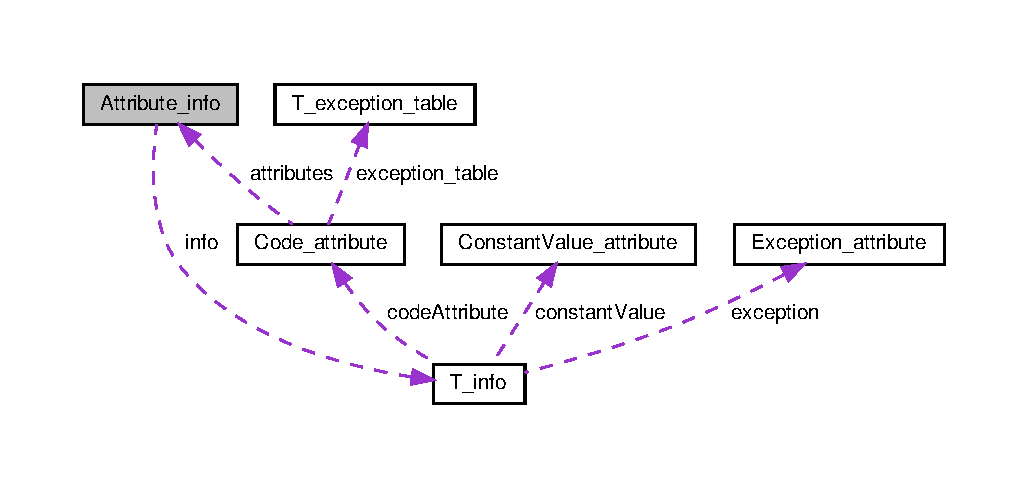
\includegraphics[width=350pt]{structAttribute__info__coll__graph}
\end{center}
\end{figure}
\subsection*{Atributos Públicos}
\begin{DoxyCompactItemize}
\item 
unsigned short \hyperlink{structAttribute__info_aa20aae72733ad98febeea64ad7927526}{name\+\_\+index}
\item 
unsigned int \hyperlink{structAttribute__info_aa76577f95471a7093757bb127f24702f}{length}
\item 
\hyperlink{unionT__info}{T\+\_\+info} $\ast$ \hyperlink{structAttribute__info_a8612e1228cbf9673986c9fee603dceca}{info}
\end{DoxyCompactItemize}


\subsection{Descrição detalhada}
Protótipo da struct \char`\"{}attribute\+\_\+info\char`\"{}. 

Estrutura de dados para salvar a posição do atributo na constantpool e seu tamanho. 

Definido na linha 74 do ficheiro Attributes.\+h.



\subsection{Documentação dos dados membro}
\mbox{\Hypertarget{structAttribute__info_a8612e1228cbf9673986c9fee603dceca}\label{structAttribute__info_a8612e1228cbf9673986c9fee603dceca}} 
\index{Attribute\+\_\+info@{Attribute\+\_\+info}!info@{info}}
\index{info@{info}!Attribute\+\_\+info@{Attribute\+\_\+info}}
\subsubsection{\texorpdfstring{info}{info}}
{\footnotesize\ttfamily \hyperlink{unionT__info}{T\+\_\+info}$\ast$ Attribute\+\_\+info\+::info}



Definido na linha 78 do ficheiro Attributes.\+h.



Referenciado por Pilha\+J\+V\+M\+::adicionar\+Frame(), gravar\+Arquivo\+Attribute(), imprimir\+Attribute(), Pilha\+J\+V\+M\+::inicializar\+P\+C(), ler\+Attribute(), Operations\+::lookupswitch(), Pilha\+J\+V\+M\+::\+Pilha\+J\+V\+M() e Operations\+::tableswitch().

\mbox{\Hypertarget{structAttribute__info_aa76577f95471a7093757bb127f24702f}\label{structAttribute__info_aa76577f95471a7093757bb127f24702f}} 
\index{Attribute\+\_\+info@{Attribute\+\_\+info}!length@{length}}
\index{length@{length}!Attribute\+\_\+info@{Attribute\+\_\+info}}
\subsubsection{\texorpdfstring{length}{length}}
{\footnotesize\ttfamily unsigned int Attribute\+\_\+info\+::length}



Definido na linha 76 do ficheiro Attributes.\+h.



Referenciado por gravar\+Arquivo\+Attribute(), imprimir\+Attribute() e ler\+Attribute().

\mbox{\Hypertarget{structAttribute__info_aa20aae72733ad98febeea64ad7927526}\label{structAttribute__info_aa20aae72733ad98febeea64ad7927526}} 
\index{Attribute\+\_\+info@{Attribute\+\_\+info}!name\+\_\+index@{name\+\_\+index}}
\index{name\+\_\+index@{name\+\_\+index}!Attribute\+\_\+info@{Attribute\+\_\+info}}
\subsubsection{\texorpdfstring{name\+\_\+index}{name\_index}}
{\footnotesize\ttfamily unsigned short Attribute\+\_\+info\+::name\+\_\+index}



Definido na linha 75 do ficheiro Attributes.\+h.



Referenciado por gravar\+Arquivo\+Attribute(), imprimir\+Attribute() e ler\+Attribute().



A documentação para esta estrutura foi gerada a partir do seguinte ficheiro\+:\begin{DoxyCompactItemize}
\item 
include/\hyperlink{Attributes_8h}{Attributes.\+h}\end{DoxyCompactItemize}

\hypertarget{classClassFile}{}\section{Referência à classe Class\+File}
\label{classClassFile}\index{Class\+File@{Class\+File}}


{\ttfamily \#include $<$Class\+File.\+h$>$}



Diagrama de colaboração para Class\+File\+:
\nopagebreak
\begin{figure}[H]
\begin{center}
\leavevmode
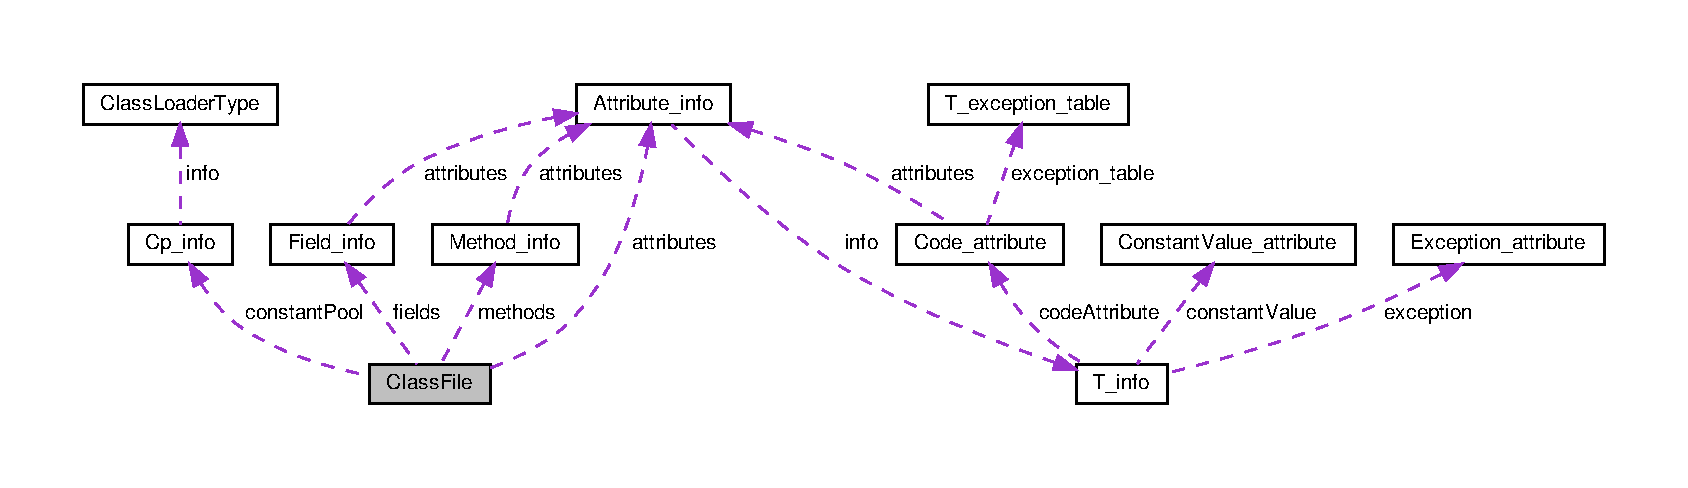
\includegraphics[width=350pt]{classClassFile__coll__graph}
\end{center}
\end{figure}
\subsection*{Membros públicos}
\begin{DoxyCompactItemize}
\item 
\hyperlink{classClassFile_a7cf76bcaf785b984e9d1b31d52a5aa7f}{Class\+File} (char $\ast$in)
\begin{DoxyCompactList}\small\item\em Construtor que configura um objeto da classe \hyperlink{classClassFile}{Class\+File} com o nome do arquivo passado. \end{DoxyCompactList}\item 
\hyperlink{classClassFile_ab442e7b0a5f8c4eeae4f668c4e02c396}{Class\+File} (string in)
\begin{DoxyCompactList}\small\item\em Construtor que configura um objeto da classe \hyperlink{classClassFile}{Class\+File} com o nome do arquivo passado. \end{DoxyCompactList}\item 
int \hyperlink{classClassFile_a5fa3d7587821ed1c8e3eabb94544da29}{inicializar\+Arquivo} (char $\ast$argv\mbox{[}$\,$\mbox{]})
\begin{DoxyCompactList}\small\item\em criar e inicializar arquivo \end{DoxyCompactList}\item 
void \hyperlink{classClassFile_a581c453009afcb8b7a2861a2de8cfb5c}{fechar\+Arquivo} ()
\begin{DoxyCompactList}\small\item\em Fechar arquivo. \end{DoxyCompactList}\item 
int \hyperlink{classClassFile_a619e102ada15202ab84981d43362a3e9}{carregar} ()
\begin{DoxyCompactList}\small\item\em Carrega o class file na classe. \end{DoxyCompactList}\item 
void \hyperlink{classClassFile_a482ed64fcd8a1b79d3622b3f59b5767a}{imprimir\+Informacoes\+Gerais} ()
\begin{DoxyCompactList}\small\item\em Imprime informações gerais do .class. \end{DoxyCompactList}\item 
void \hyperlink{classClassFile_a4a685afd10dc5aaacd5a71ed535895c6}{gravar\+Arquivo\+Informacoes\+Gerais} ()
\begin{DoxyCompactList}\small\item\em Gravar informações gerais do .class em um arquivo. \end{DoxyCompactList}\item 
bool \hyperlink{classClassFile_a7da7cc6de8de3fc6f27faf3b76f4883a}{exibir} ()
\begin{DoxyCompactList}\small\item\em Imprime todas as informações do .class. \end{DoxyCompactList}\item 
bool \hyperlink{classClassFile_a452169cb59d63012f98a34a3fff2c2f7}{gravar\+Arquivo} ()
\begin{DoxyCompactList}\small\item\em Gravar todas as informações do .class em um arquivo. \end{DoxyCompactList}\item 
bool \hyperlink{classClassFile_a8dd042ff6873b9f0d16f8ee3812261e1}{validar\+Extensao} ()
\begin{DoxyCompactList}\small\item\em Verifica se a extensão do arquivo é .class. \end{DoxyCompactList}\item 
bool \hyperlink{classClassFile_a10bfe22492b473fb0197e55f451978e5}{existe\+Main} ()
\begin{DoxyCompactList}\small\item\em Verifica se o .class possui função main. \end{DoxyCompactList}\item 
\hyperlink{structMethod__info}{Method\+\_\+info} \hyperlink{classClassFile_afdbe9cc2f360e04273470202c4f247dc}{obter\+Main} ()
\begin{DoxyCompactList}\small\item\em Retorna o método main. \end{DoxyCompactList}\item 
bool \hyperlink{classClassFile_a2a886bdb4c42bfaaf5ea8ff1b2c41209}{existe\+Clinit} ()
\begin{DoxyCompactList}\small\item\em Verifica se o .class tem o método clinit. \end{DoxyCompactList}\item 
\hyperlink{structMethod__info}{Method\+\_\+info} \hyperlink{classClassFile_a1141f5a8c856d5f3931f0b518e219f79}{obter\+Clinit} ()
\begin{DoxyCompactList}\small\item\em Retorna o método clinit. \end{DoxyCompactList}\item 
bool \hyperlink{classClassFile_a6b8f23db0ee4af80a2e75d46a191dc20}{verificar\+This\+Class} ()
\begin{DoxyCompactList}\small\item\em Verifica se a class definida é igual ao nome da classe sem extensões. \end{DoxyCompactList}\item 
int \hyperlink{classClassFile_a170339cd16cf0afc0567865b3f372d38}{obter\+Status} ()
\begin{DoxyCompactList}\small\item\em Retorna o status lido, informando para o método que chamou o que aconteceu. \end{DoxyCompactList}\item 
\hyperlink{structCp__info}{Cp\+\_\+info} $\ast$ \hyperlink{classClassFile_ab70fe581c4b7a1824adf490c3a53bcc7}{obter\+Constant\+Pool} () const
\begin{DoxyCompactList}\small\item\em Retorna referencia a constant pool. \end{DoxyCompactList}\item 
\hyperlink{BasicTypes_8h_a90240657108b1b457eef9d3f76e0202e}{U2} \hyperlink{classClassFile_a8b60418144c498b9d9545b1784bddf21}{obter\+Tamanho\+Constant\+Pool} ()
\begin{DoxyCompactList}\small\item\em Retorna o valor do tamanho da constant pool. \end{DoxyCompactList}\item 
char $\ast$ \hyperlink{classClassFile_a4803bd3f325fbab1bf9c0f774b3a8c97}{obter\+Path} ()
\begin{DoxyCompactList}\small\item\em Pega o caminho do arquivo .class. \end{DoxyCompactList}\item 
\hyperlink{structMethod__info}{Method\+\_\+info} $\ast$ \hyperlink{classClassFile_a6ecce8d87f74c84b07f102c0298de13a}{obter\+Methods} ()
\begin{DoxyCompactList}\small\item\em Retorna todos os métodos. \end{DoxyCompactList}\item 
\hyperlink{BasicTypes_8h_a90240657108b1b457eef9d3f76e0202e}{U2} \hyperlink{classClassFile_a16409bc8b58eb4965a1e39497cc300d8}{obter\+Methods\+Count} ()
\begin{DoxyCompactList}\small\item\em Retorna o numero de Methods. \end{DoxyCompactList}\item 
\hyperlink{BasicTypes_8h_a90240657108b1b457eef9d3f76e0202e}{U2} \hyperlink{classClassFile_aec88c5432526d16b546ed59e5cec2136}{obter\+This\+\_\+class} ()
\begin{DoxyCompactList}\small\item\em Retorna um índice da constant pool que aponta para string com nome da class. \end{DoxyCompactList}\item 
\hyperlink{BasicTypes_8h_a90240657108b1b457eef9d3f76e0202e}{U2} \hyperlink{classClassFile_a8f248001f388181db10e76602031d560}{obter\+Super\+\_\+class} ()
\begin{DoxyCompactList}\small\item\em Retorna um índice da constant pool que aponta para string com nome da superclass. \end{DoxyCompactList}\item 
\hyperlink{BasicTypes_8h_a90240657108b1b457eef9d3f76e0202e}{U2} \hyperlink{classClassFile_a0be559cd8b7b3168c81a2782e4facb0c}{obter\+Fields\+Count} ()
\begin{DoxyCompactList}\small\item\em Retorna número de fields. \end{DoxyCompactList}\item 
\hyperlink{structField__info}{Field\+\_\+info} $\ast$ \hyperlink{classClassFile_ac3aabaa918413884416692b29165b463}{obter\+Fields} ()
\begin{DoxyCompactList}\small\item\em Retorna a array com as fields lidas. \end{DoxyCompactList}\item 
\hyperlink{structField__info}{Field\+\_\+info} $\ast$ \hyperlink{classClassFile_a1ae90b1662ca222c9910c14997b20eaa}{obter\+Field} (string nome)
\begin{DoxyCompactList}\small\item\em Retorna um field. \end{DoxyCompactList}\item 
\hyperlink{structMethod__info}{Method\+\_\+info} $\ast$ \hyperlink{classClassFile_aac49e7e39f677987b53fdf15787b8106}{obter\+Method} (string nome, string descriptor)
\item 
\hyperlink{classClassFile}{Class\+File} $\ast$ \hyperlink{classClassFile_a4d0ac62c4d6218ddada33f715ebaf633}{obter\+Class\+That\+Has\+Serached\+Method} (string nome, string descriptor)
\begin{DoxyCompactList}\small\item\em Retorna o ponteiro para o leitor do .class que contém o método encontrado em get\+Method. \end{DoxyCompactList}\item 
int \hyperlink{classClassFile_acdb7018a6926b187bc6ecc18abf0fff8}{validacao} (void)
\begin{DoxyCompactList}\small\item\em Valida estrutura obrigatoria. \end{DoxyCompactList}\end{DoxyCompactItemize}
\subsection*{Membros privados}
\begin{DoxyCompactItemize}
\item 
bool \hyperlink{classClassFile_ae8e4445e763c4ee7c04995fcea0369e0}{verificar\+Main} ()
\begin{DoxyCompactList}\small\item\em Encontro em qual method está a main. \end{DoxyCompactList}\item 
bool \hyperlink{classClassFile_ab0394185a299f35a9b5be68143385e84}{verificar\+Clinit} ()
\begin{DoxyCompactList}\small\item\em Encontra em qual method esta a clinit, se existir. \end{DoxyCompactList}\item 
string \hyperlink{classClassFile_a32767b8d966ef87249aa3a41ec5d67c3}{obter\+Erro} (int erro)
\begin{DoxyCompactList}\small\item\em Retorna a string que contém uma mensagem de erro correspondente ao índice que recebe como parâmetro. \end{DoxyCompactList}\end{DoxyCompactItemize}
\subsection*{Atributos Privados}
\begin{DoxyCompactItemize}
\item 
int \hyperlink{classClassFile_a9afeae9ac0889ab75909e73933e29326}{status}
\item 
int \hyperlink{classClassFile_ac1cdef340faa0bd945b2236057433978}{main\+Method}
\item 
int \hyperlink{classClassFile_aa1eb77ebbd737bde7edde5fbdb2b6992}{clinit}
\item 
bool \hyperlink{classClassFile_ad8d08e096c470901c62d1a9e31a202bf}{encontrou\+Main}
\item 
bool \hyperlink{classClassFile_a5c60c8d51584f48f22bdbdd719960e05}{encontrou\+Clinit}
\item 
char $\ast$ \hyperlink{classClassFile_a2789cf19be5abaeadf96f83de33174a4}{file\+Name}
\item 
\hyperlink{BasicTypes_8h_a90240657108b1b457eef9d3f76e0202e}{U2} \hyperlink{classClassFile_ab0d3a4474a9907dc61893d0293525b38}{min\+Version}
\item 
\hyperlink{BasicTypes_8h_a90240657108b1b457eef9d3f76e0202e}{U2} \hyperlink{classClassFile_a40bd108a13debb86701cf31742572686}{maj\+Version}
\item 
\hyperlink{BasicTypes_8h_a90240657108b1b457eef9d3f76e0202e}{U2} \hyperlink{classClassFile_acde5006251ffd25149efa4d6fb725cf5}{length\+CP}
\item 
\hyperlink{BasicTypes_8h_a90240657108b1b457eef9d3f76e0202e}{U2} \hyperlink{classClassFile_a205bc5af050f4676fc4c3ff7992c4959}{this\+\_\+class}
\item 
\hyperlink{BasicTypes_8h_a90240657108b1b457eef9d3f76e0202e}{U2} \hyperlink{classClassFile_ad92079216f8cdb366a3002e5ca2c2dfa}{super\+\_\+class}
\item 
\hyperlink{BasicTypes_8h_a90240657108b1b457eef9d3f76e0202e}{U2} \hyperlink{classClassFile_a1bbca13f93ec21beffa8a56e360c9f8d}{interfaces\+Count}
\item 
\hyperlink{BasicTypes_8h_a90240657108b1b457eef9d3f76e0202e}{U2} \hyperlink{classClassFile_a5eae2e906695e596b89614df0e4b060a}{fields\+Count}
\item 
\hyperlink{BasicTypes_8h_a90240657108b1b457eef9d3f76e0202e}{U2} \hyperlink{classClassFile_a4c362d4adfeaad02f4517caf1ba58103}{methods\+Count}
\item 
\hyperlink{BasicTypes_8h_a90240657108b1b457eef9d3f76e0202e}{U2} \hyperlink{classClassFile_a16d2ca3e9cdf9267adde08575c57bfa9}{access\+Flags}
\item 
\hyperlink{BasicTypes_8h_a90240657108b1b457eef9d3f76e0202e}{U2} \hyperlink{classClassFile_a66691e77df3f8604eebebc8759953542}{attributes\+Count}
\item 
\hyperlink{BasicTypes_8h_a90240657108b1b457eef9d3f76e0202e}{U2} $\ast$ \hyperlink{classClassFile_a94d1e4e835476f47e3a8b81ecd0301c0}{interfaces}
\item 
\hyperlink{structCp__info}{Cp\+\_\+info} $\ast$ \hyperlink{classClassFile_a5883215e48e253a84c105a18d34049ca}{constant\+Pool}
\item 
\hyperlink{structField__info}{Field\+\_\+info} $\ast$ \hyperlink{classClassFile_a6d6ec8aa668982ea722edc40b3ea5b1a}{fields}
\item 
\hyperlink{structMethod__info}{Method\+\_\+info} $\ast$ \hyperlink{classClassFile_a5906980e6c5121e5a864346fd3617083}{methods}
\item 
\hyperlink{structAttribute__info}{Attribute\+\_\+info} $\ast$ \hyperlink{classClassFile_a20d4b18030becbd8df5b7584477e94b6}{attributes}
\item 
F\+I\+LE $\ast$ \hyperlink{classClassFile_ae2be12dcc1a042970b4d7d7cf9709624}{arquivo\+Class}
\item 
fstream \hyperlink{classClassFile_a4aee6c7763d46884d5b2c0297142df99}{arquivo\+Saida}
\end{DoxyCompactItemize}


\subsection{Descrição detalhada}
\hypertarget{classClassFile_DESCRIPTION}{}\subsection{D\+E\+S\+C\+R\+I\+P\+T\+I\+ON}\label{classClassFile_DESCRIPTION}
A classe \hyperlink{classClassFile}{Class\+File} contém os bytecodes armazenados em memoria 

Definido na linha 48 do ficheiro Class\+File.\+h.



\subsection{Documentação dos Construtores \& Destrutor}
\mbox{\Hypertarget{classClassFile_a7cf76bcaf785b984e9d1b31d52a5aa7f}\label{classClassFile_a7cf76bcaf785b984e9d1b31d52a5aa7f}} 
\index{Class\+File@{Class\+File}!Class\+File@{Class\+File}}
\index{Class\+File@{Class\+File}!Class\+File@{Class\+File}}
\subsubsection{\texorpdfstring{Class\+File()}{ClassFile()}\hspace{0.1cm}{\footnotesize\ttfamily [1/2]}}
{\footnotesize\ttfamily Class\+File\+::\+Class\+File (\begin{DoxyParamCaption}\item[{char $\ast$}]{in }\end{DoxyParamCaption})}



Construtor que configura um objeto da classe \hyperlink{classClassFile}{Class\+File} com o nome do arquivo passado. 


\begin{DoxyParams}{Parâmetros}
{\em in} & caminho do arquivo .class. \\
\hline
\end{DoxyParams}


Definido na linha 8 do ficheiro Class\+File.\+cpp.



Referências file\+Name e status.

\mbox{\Hypertarget{classClassFile_ab442e7b0a5f8c4eeae4f668c4e02c396}\label{classClassFile_ab442e7b0a5f8c4eeae4f668c4e02c396}} 
\index{Class\+File@{Class\+File}!Class\+File@{Class\+File}}
\index{Class\+File@{Class\+File}!Class\+File@{Class\+File}}
\subsubsection{\texorpdfstring{Class\+File()}{ClassFile()}\hspace{0.1cm}{\footnotesize\ttfamily [2/2]}}
{\footnotesize\ttfamily Class\+File\+::\+Class\+File (\begin{DoxyParamCaption}\item[{string}]{in }\end{DoxyParamCaption})}



Construtor que configura um objeto da classe \hyperlink{classClassFile}{Class\+File} com o nome do arquivo passado. 


\begin{DoxyParams}{Parâmetros}
{\em in} & caminho do arquivo .class. \\
\hline
\end{DoxyParams}


Definido na linha 15 do ficheiro Class\+File.\+cpp.



Referências file\+Name e status.



\subsection{Documentação dos métodos}
\mbox{\Hypertarget{classClassFile_a619e102ada15202ab84981d43362a3e9}\label{classClassFile_a619e102ada15202ab84981d43362a3e9}} 
\index{Class\+File@{Class\+File}!carregar@{carregar}}
\index{carregar@{carregar}!Class\+File@{Class\+File}}
\subsubsection{\texorpdfstring{carregar()}{carregar()}}
{\footnotesize\ttfamily int Class\+File\+::carregar (\begin{DoxyParamCaption}{ }\end{DoxyParamCaption})}



Carrega o class file na classe. 

\begin{DoxyReturn}{Retorna}
variavel status que indica se houve erro no programa 
\end{DoxyReturn}


Definido na linha 68 do ficheiro Class\+File.\+cpp.



Referências access\+Flags, arquivo\+Class, attributes, attributes\+Count, C\+A\+N\+T\+\_\+\+O\+P\+EN, carregar\+Constant\+Pool(), constant\+Pool, encontrou\+Clinit, encontrou\+Main, fields, fields\+Count, file\+Name, interfaces, interfaces\+Count, I\+N\+V\+A\+L\+I\+D\+\_\+\+E\+X\+T\+E\+N\+S\+I\+ON, I\+N\+V\+A\+L\+I\+D\+\_\+\+F\+I\+LE, I\+N\+V\+A\+L\+I\+D\+\_\+\+N\+A\+ME, length\+CP, ler\+Todas\+Interfaces(), ler\+Todos\+Attributes(), ler\+Todos\+Fields(), ler\+Todos\+Methods(), ler\+U2(), ler\+U4(), maj\+Version, methods, methods\+Count, min\+Version, M\+I\+S\+S\+I\+N\+G\+\_\+\+A\+R\+G\+U\+M\+E\+NT, obter\+Erro(), status, super\+\_\+class, this\+\_\+class, U\+N\+K\+N\+O\+W\+N\+\_\+\+T\+Y\+PE, validar\+Extensao(), verificar\+Clinit(), verificar\+Main() e verificar\+This\+Class().



Referenciado por Method\+Area\+::adicionar\+Classe() e main().

Grafo de chamadas desta função\+:
\nopagebreak
\begin{figure}[H]
\begin{center}
\leavevmode
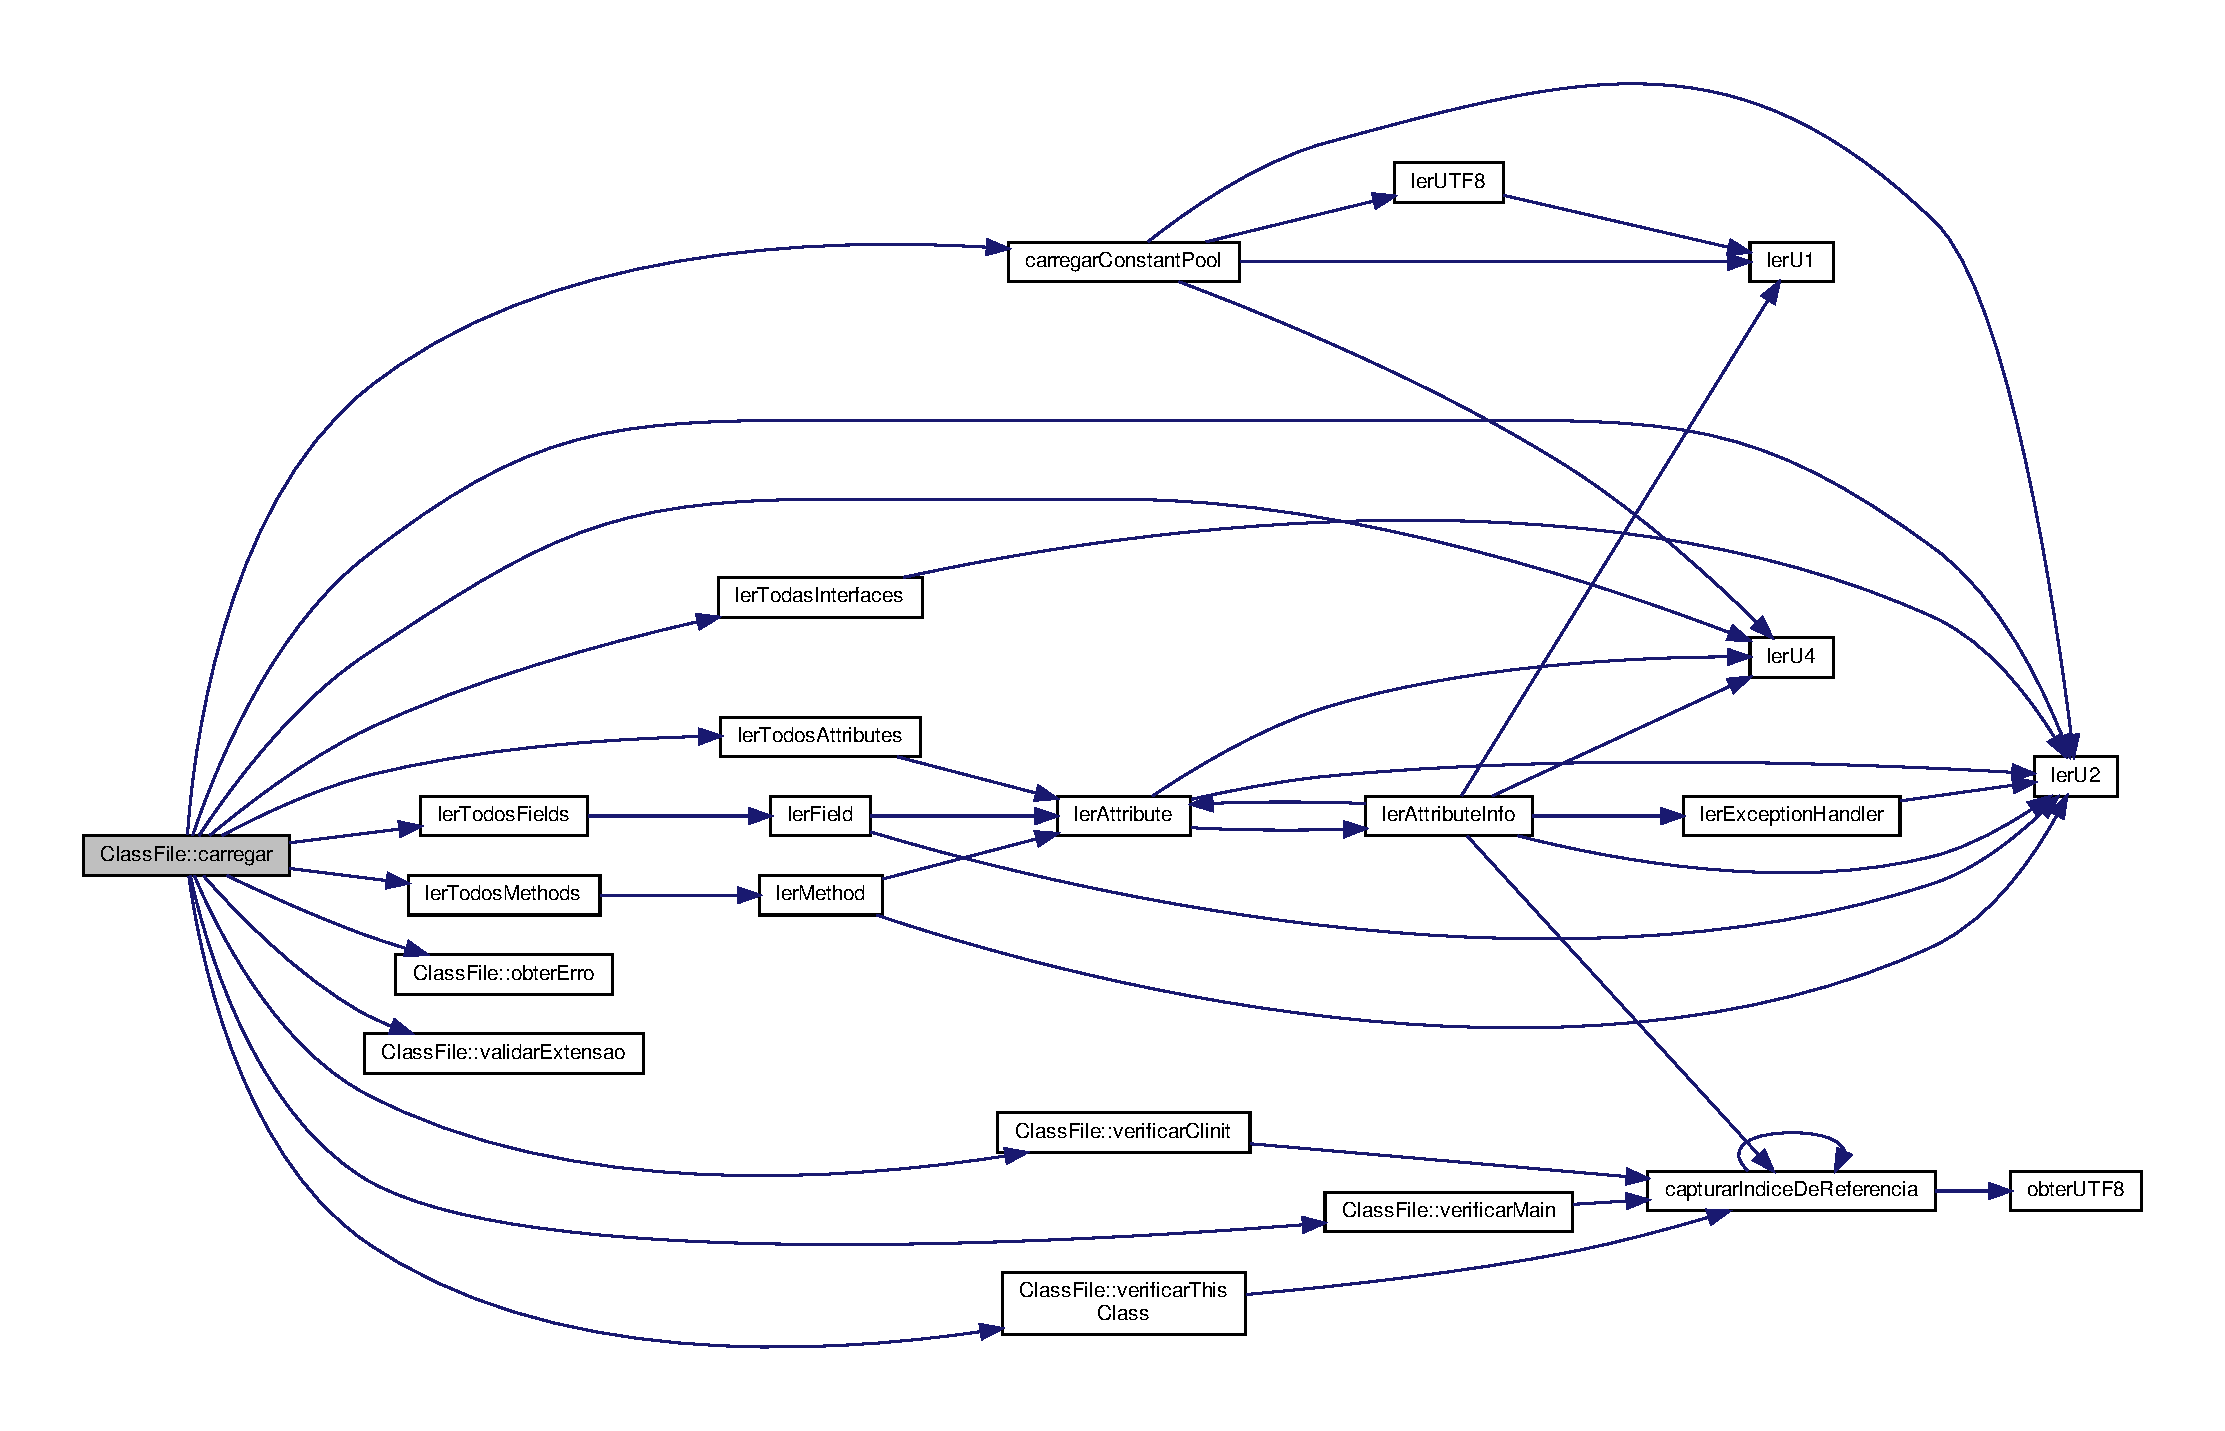
\includegraphics[width=350pt]{classClassFile_a619e102ada15202ab84981d43362a3e9_cgraph}
\end{center}
\end{figure}
\mbox{\Hypertarget{classClassFile_a7da7cc6de8de3fc6f27faf3b76f4883a}\label{classClassFile_a7da7cc6de8de3fc6f27faf3b76f4883a}} 
\index{Class\+File@{Class\+File}!exibir@{exibir}}
\index{exibir@{exibir}!Class\+File@{Class\+File}}
\subsubsection{\texorpdfstring{exibir()}{exibir()}}
{\footnotesize\ttfamily bool Class\+File\+::exibir (\begin{DoxyParamCaption}{ }\end{DoxyParamCaption})}



Imprime todas as informações do .class. 

\begin{DoxyReturn}{Retorna}
true ou false dependendo se a variavel status indicar que houve erro na leitura 
\end{DoxyReturn}


Definido na linha 176 do ficheiro Class\+File.\+cpp.



Referências attributes, attributes\+Count, constant\+Pool, fields, fields\+Count, imprimir\+Constant\+Pool(), imprimir\+Informacoes\+Gerais(), imprimir\+Todas\+Interfaces(), imprimir\+Todos\+Attributes(), imprimir\+Todos\+Field(), imprimir\+Todos\+Methods(), interfaces, interfaces\+Count, length\+CP, methods, methods\+Count e status.



Referenciado por main().

Grafo de chamadas desta função\+:
\nopagebreak
\begin{figure}[H]
\begin{center}
\leavevmode
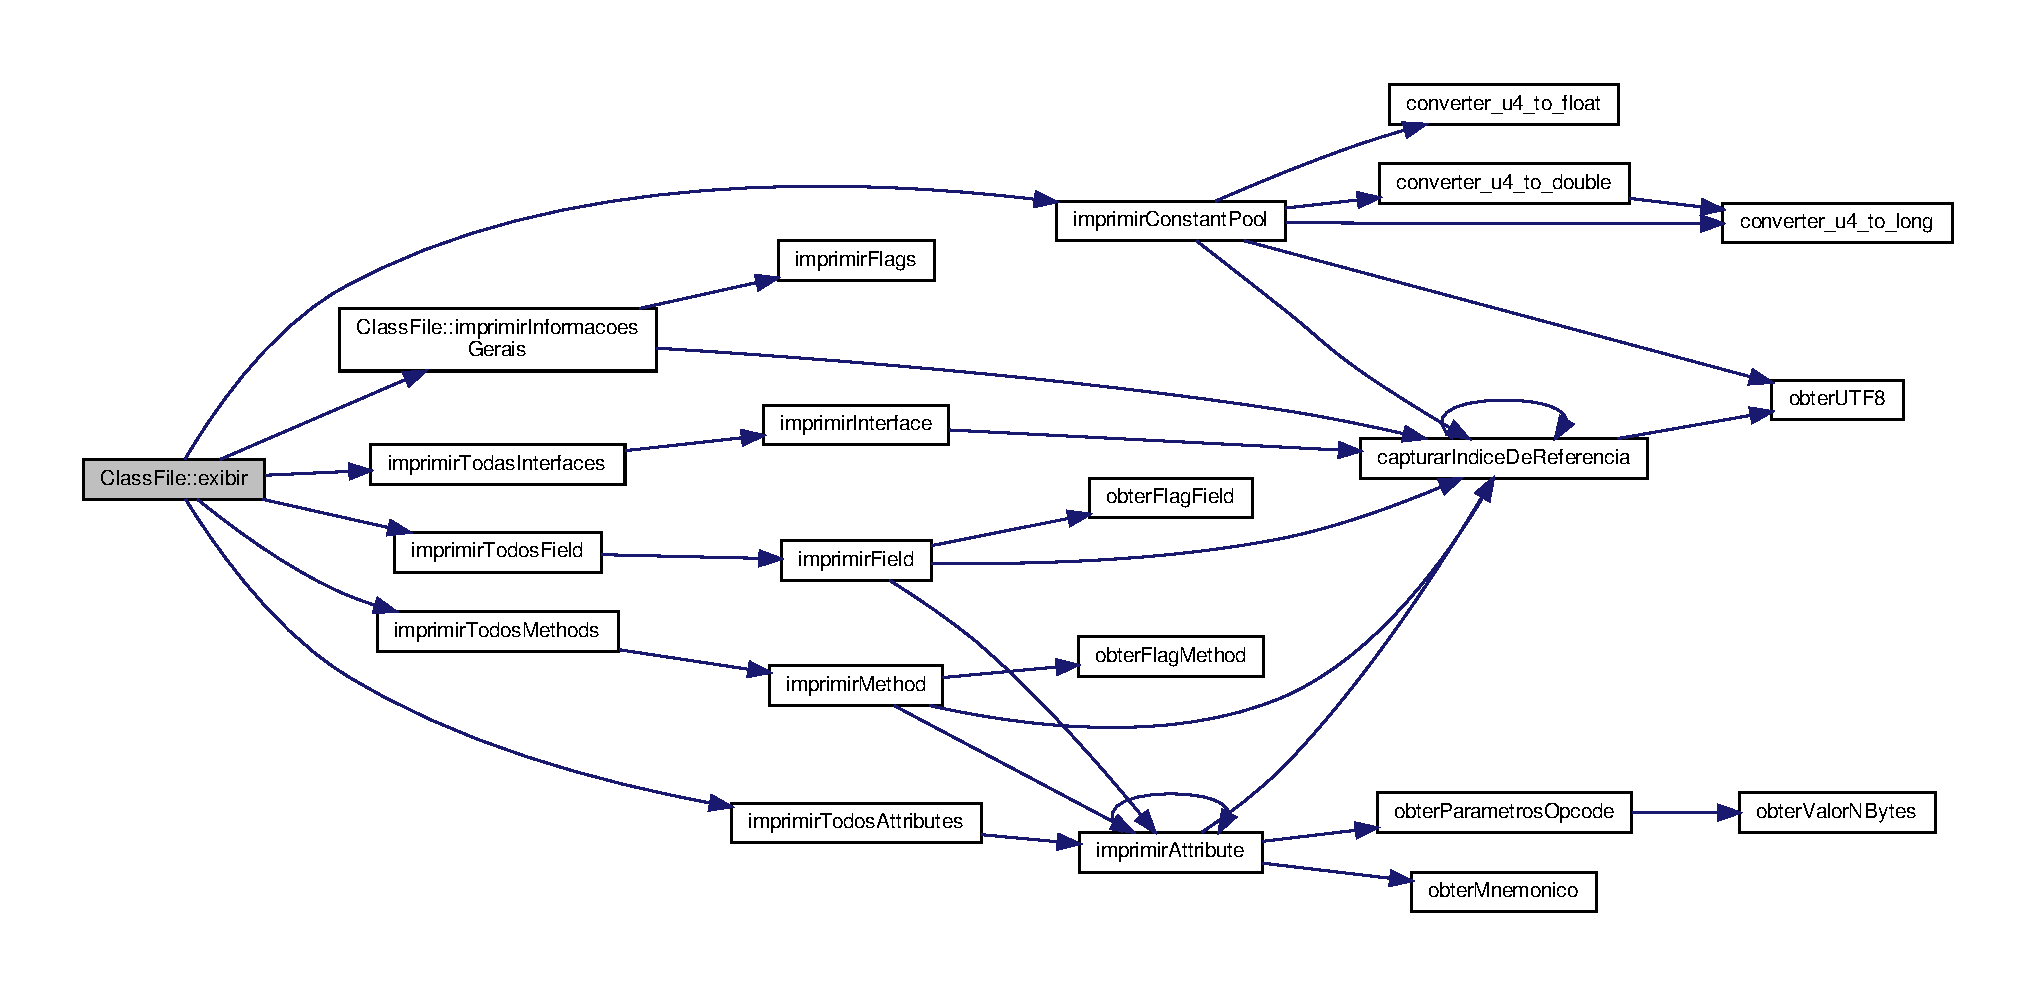
\includegraphics[width=350pt]{classClassFile_a7da7cc6de8de3fc6f27faf3b76f4883a_cgraph}
\end{center}
\end{figure}
\mbox{\Hypertarget{classClassFile_a2a886bdb4c42bfaaf5ea8ff1b2c41209}\label{classClassFile_a2a886bdb4c42bfaaf5ea8ff1b2c41209}} 
\index{Class\+File@{Class\+File}!existe\+Clinit@{existe\+Clinit}}
\index{existe\+Clinit@{existe\+Clinit}!Class\+File@{Class\+File}}
\subsubsection{\texorpdfstring{existe\+Clinit()}{existeClinit()}}
{\footnotesize\ttfamily bool Class\+File\+::existe\+Clinit (\begin{DoxyParamCaption}{ }\end{DoxyParamCaption})}



Verifica se o .class tem o método clinit. 

\begin{DoxyReturn}{Retorna}
booleano que indica se existe o metodo clinit 
\end{DoxyReturn}


Definido na linha 344 do ficheiro Class\+File.\+cpp.



Referências encontrou\+Clinit e verificar\+Clinit().



Referenciado por Method\+Area\+::adicionar\+Classe().

Grafo de chamadas desta função\+:
\nopagebreak
\begin{figure}[H]
\begin{center}
\leavevmode
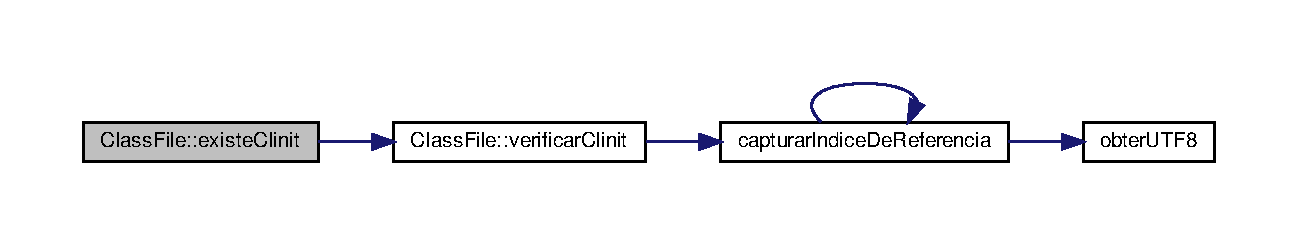
\includegraphics[width=350pt]{classClassFile_a2a886bdb4c42bfaaf5ea8ff1b2c41209_cgraph}
\end{center}
\end{figure}
\mbox{\Hypertarget{classClassFile_a10bfe22492b473fb0197e55f451978e5}\label{classClassFile_a10bfe22492b473fb0197e55f451978e5}} 
\index{Class\+File@{Class\+File}!existe\+Main@{existe\+Main}}
\index{existe\+Main@{existe\+Main}!Class\+File@{Class\+File}}
\subsubsection{\texorpdfstring{existe\+Main()}{existeMain()}}
{\footnotesize\ttfamily bool Class\+File\+::existe\+Main (\begin{DoxyParamCaption}{ }\end{DoxyParamCaption})}



Verifica se o .class possui função main. 

\begin{DoxyReturn}{Retorna}
booleano que indica se existe o metodo main 
\end{DoxyReturn}


Definido na linha 338 do ficheiro Class\+File.\+cpp.



Referências encontrou\+Main e verificar\+Main().

Grafo de chamadas desta função\+:
\nopagebreak
\begin{figure}[H]
\begin{center}
\leavevmode
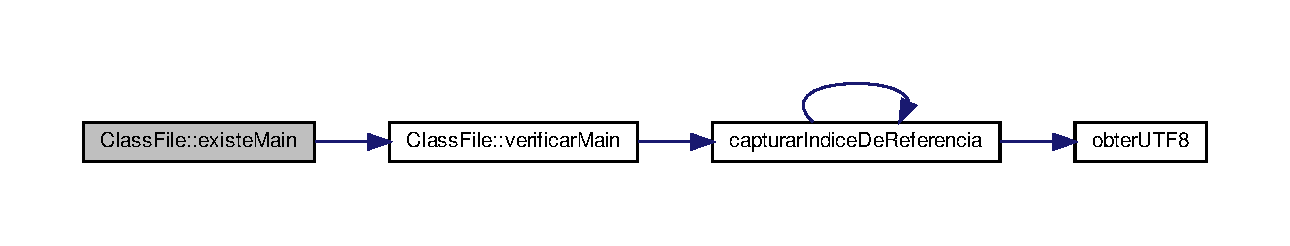
\includegraphics[width=350pt]{classClassFile_a10bfe22492b473fb0197e55f451978e5_cgraph}
\end{center}
\end{figure}
\mbox{\Hypertarget{classClassFile_a581c453009afcb8b7a2861a2de8cfb5c}\label{classClassFile_a581c453009afcb8b7a2861a2de8cfb5c}} 
\index{Class\+File@{Class\+File}!fechar\+Arquivo@{fechar\+Arquivo}}
\index{fechar\+Arquivo@{fechar\+Arquivo}!Class\+File@{Class\+File}}
\subsubsection{\texorpdfstring{fechar\+Arquivo()}{fecharArquivo()}}
{\footnotesize\ttfamily void Class\+File\+::fechar\+Arquivo (\begin{DoxyParamCaption}{ }\end{DoxyParamCaption})}



Fechar arquivo. 



Definido na linha 41 do ficheiro Class\+File.\+cpp.



Referências arquivo\+Saida.



Referenciado por main().

\mbox{\Hypertarget{classClassFile_a452169cb59d63012f98a34a3fff2c2f7}\label{classClassFile_a452169cb59d63012f98a34a3fff2c2f7}} 
\index{Class\+File@{Class\+File}!gravar\+Arquivo@{gravar\+Arquivo}}
\index{gravar\+Arquivo@{gravar\+Arquivo}!Class\+File@{Class\+File}}
\subsubsection{\texorpdfstring{gravar\+Arquivo()}{gravarArquivo()}}
{\footnotesize\ttfamily bool Class\+File\+::gravar\+Arquivo (\begin{DoxyParamCaption}{ }\end{DoxyParamCaption})}



Gravar todas as informações do .class em um arquivo. 

\begin{DoxyReturn}{Retorna}
true ou false dependendo se a variavel status indicar que houve erro na leitura 
\end{DoxyReturn}


Definido na linha 203 do ficheiro Class\+File.\+cpp.



Referências arquivo\+Saida, attributes, attributes\+Count, constant\+Pool, fields, fields\+Count, gravar\+Arquivo\+Constant\+Pool(), gravar\+Arquivo\+Informacoes\+Gerais(), gravar\+Arquivo\+Todas\+Interfaces(), gravar\+Arquivo\+Todos\+Attributes(), gravar\+Arquivo\+Todos\+Field(), gravar\+Arquivo\+Todos\+Methods(), interfaces, interfaces\+Count, length\+CP, methods, methods\+Count e status.



Referenciado por main().

Grafo de chamadas desta função\+:
\nopagebreak
\begin{figure}[H]
\begin{center}
\leavevmode
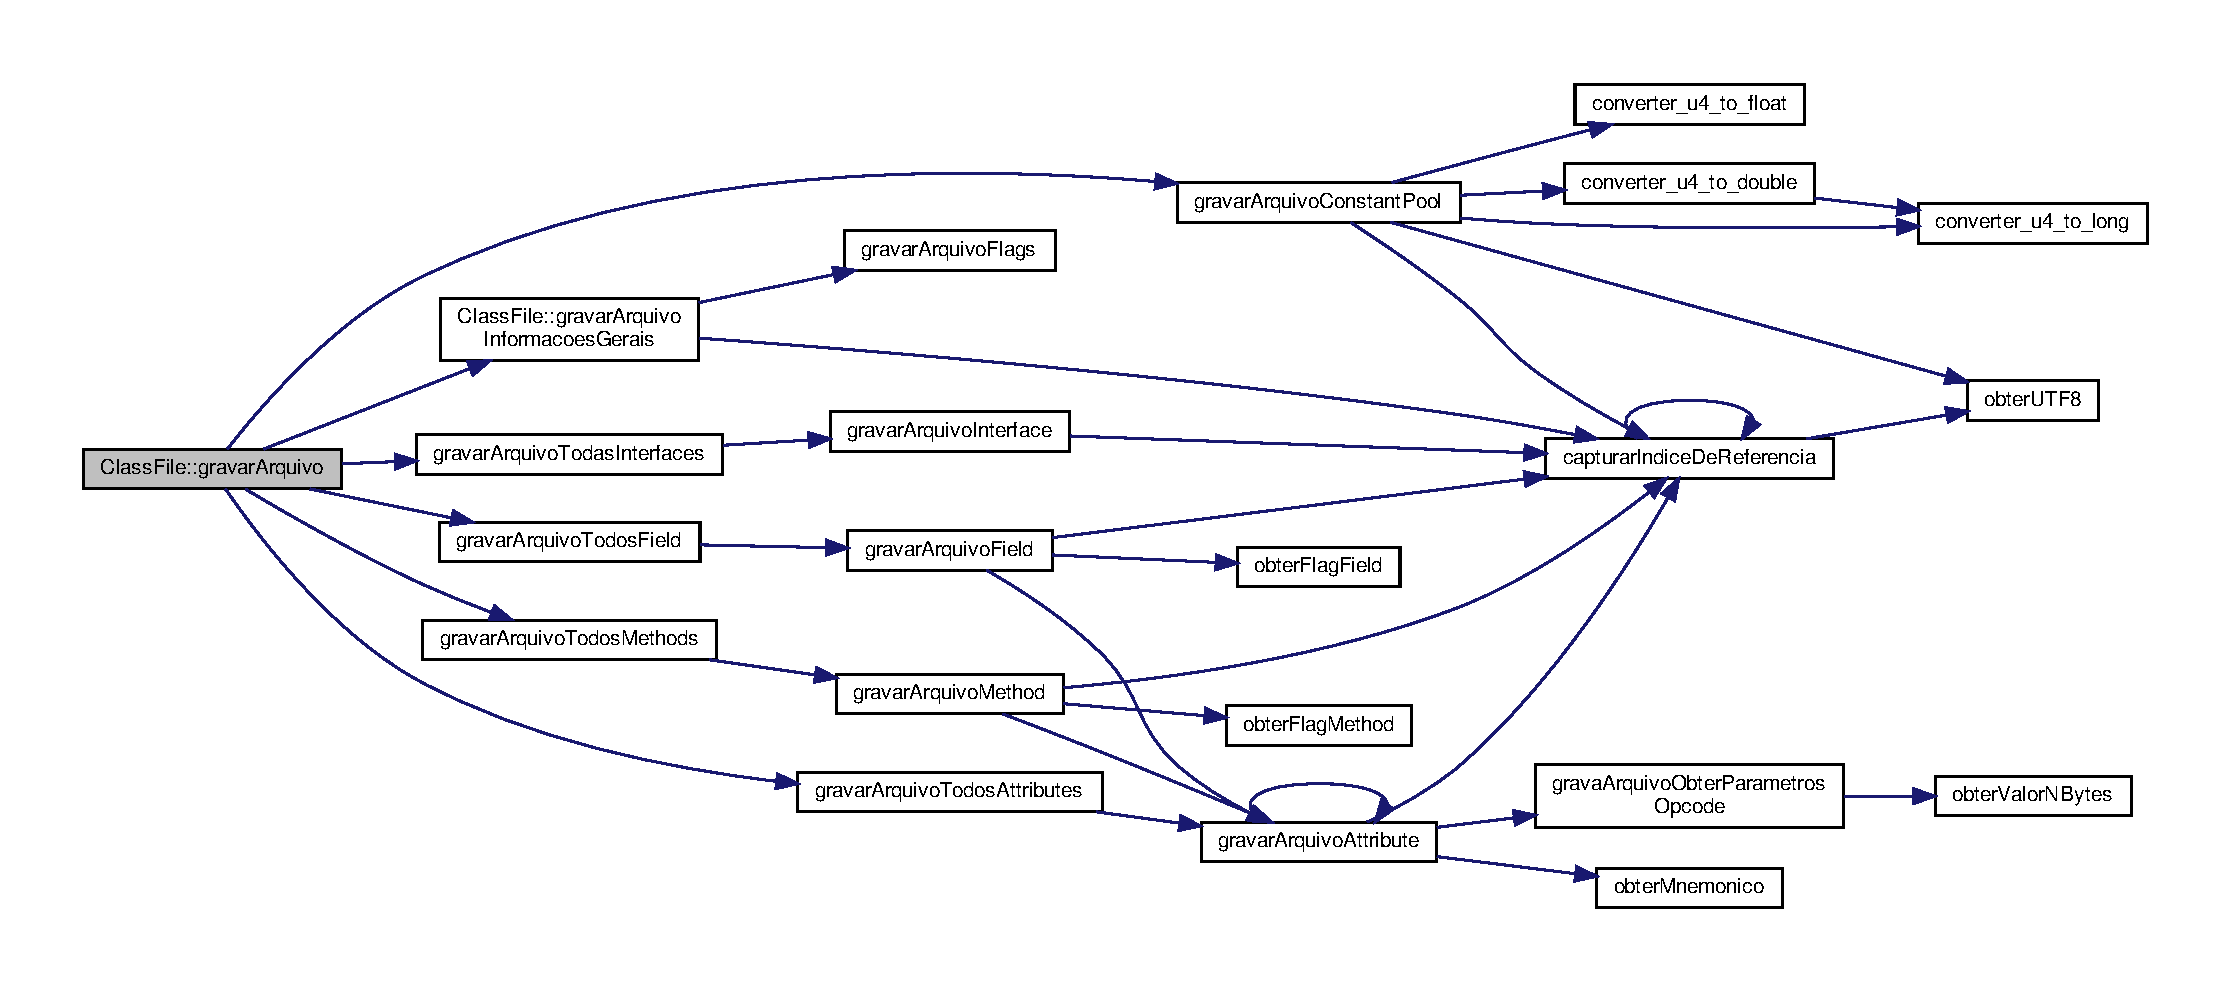
\includegraphics[width=350pt]{classClassFile_a452169cb59d63012f98a34a3fff2c2f7_cgraph}
\end{center}
\end{figure}
\mbox{\Hypertarget{classClassFile_a4a685afd10dc5aaacd5a71ed535895c6}\label{classClassFile_a4a685afd10dc5aaacd5a71ed535895c6}} 
\index{Class\+File@{Class\+File}!gravar\+Arquivo\+Informacoes\+Gerais@{gravar\+Arquivo\+Informacoes\+Gerais}}
\index{gravar\+Arquivo\+Informacoes\+Gerais@{gravar\+Arquivo\+Informacoes\+Gerais}!Class\+File@{Class\+File}}
\subsubsection{\texorpdfstring{gravar\+Arquivo\+Informacoes\+Gerais()}{gravarArquivoInformacoesGerais()}}
{\footnotesize\ttfamily bool Class\+File\+::gravar\+Arquivo\+Informacoes\+Gerais (\begin{DoxyParamCaption}{ }\end{DoxyParamCaption})}



Gravar informações gerais do .class em um arquivo. 

\begin{DoxyReturn}{Retorna}
variavel status que indica se houve erro no programa 
\end{DoxyReturn}


Definido na linha 253 do ficheiro Class\+File.\+cpp.



Referências access\+Flags, arquivo\+Saida, attributes\+Count, capturar\+Indice\+De\+Referencia(), constant\+Pool, fields\+Count, gravar\+Arquivo\+Flags(), interfaces\+Count, length\+CP, maj\+Version, methods\+Count, min\+Version, super\+\_\+class e this\+\_\+class.



Referenciado por gravar\+Arquivo().

Grafo de chamadas desta função\+:
\nopagebreak
\begin{figure}[H]
\begin{center}
\leavevmode
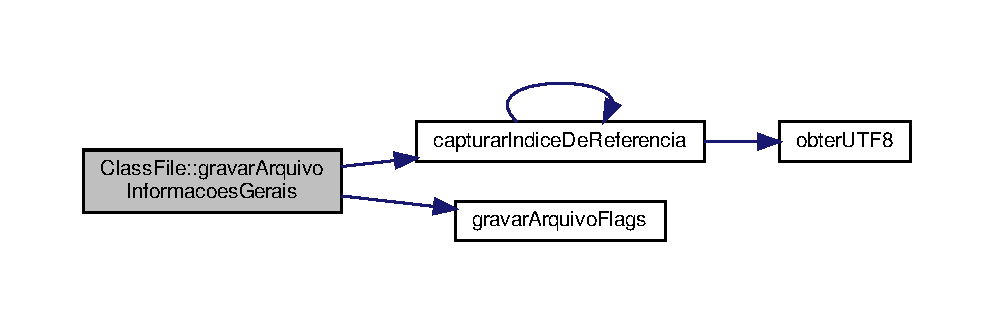
\includegraphics[width=350pt]{classClassFile_a4a685afd10dc5aaacd5a71ed535895c6_cgraph}
\end{center}
\end{figure}
\mbox{\Hypertarget{classClassFile_a482ed64fcd8a1b79d3622b3f59b5767a}\label{classClassFile_a482ed64fcd8a1b79d3622b3f59b5767a}} 
\index{Class\+File@{Class\+File}!imprimir\+Informacoes\+Gerais@{imprimir\+Informacoes\+Gerais}}
\index{imprimir\+Informacoes\+Gerais@{imprimir\+Informacoes\+Gerais}!Class\+File@{Class\+File}}
\subsubsection{\texorpdfstring{imprimir\+Informacoes\+Gerais()}{imprimirInformacoesGerais()}}
{\footnotesize\ttfamily bool Class\+File\+::imprimir\+Informacoes\+Gerais (\begin{DoxyParamCaption}{ }\end{DoxyParamCaption})}



Imprime informações gerais do .class. 

\begin{DoxyReturn}{Retorna}
variavel status que indica se houve erro no programa 
\end{DoxyReturn}


Definido na linha 224 do ficheiro Class\+File.\+cpp.



Referências access\+Flags, attributes\+Count, capturar\+Indice\+De\+Referencia(), constant\+Pool, fields\+Count, imprimir\+Flags(), interfaces\+Count, length\+CP, maj\+Version, methods\+Count, min\+Version, super\+\_\+class e this\+\_\+class.



Referenciado por exibir().

Grafo de chamadas desta função\+:
\nopagebreak
\begin{figure}[H]
\begin{center}
\leavevmode
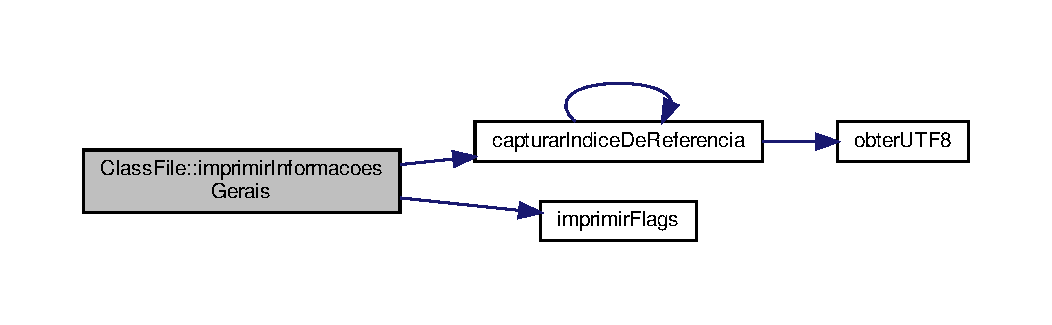
\includegraphics[width=350pt]{classClassFile_a482ed64fcd8a1b79d3622b3f59b5767a_cgraph}
\end{center}
\end{figure}
\mbox{\Hypertarget{classClassFile_a5fa3d7587821ed1c8e3eabb94544da29}\label{classClassFile_a5fa3d7587821ed1c8e3eabb94544da29}} 
\index{Class\+File@{Class\+File}!inicializar\+Arquivo@{inicializar\+Arquivo}}
\index{inicializar\+Arquivo@{inicializar\+Arquivo}!Class\+File@{Class\+File}}
\subsubsection{\texorpdfstring{inicializar\+Arquivo()}{inicializarArquivo()}}
{\footnotesize\ttfamily int Class\+File\+::inicializar\+Arquivo (\begin{DoxyParamCaption}\item[{char $\ast$}]{argv\mbox{[}$\,$\mbox{]} }\end{DoxyParamCaption})}



criar e inicializar arquivo 



Definido na linha 27 do ficheiro Class\+File.\+cpp.



Referências arquivo\+Saida e status.



Referenciado por main().

\mbox{\Hypertarget{classClassFile_a4d0ac62c4d6218ddada33f715ebaf633}\label{classClassFile_a4d0ac62c4d6218ddada33f715ebaf633}} 
\index{Class\+File@{Class\+File}!obter\+Class\+That\+Has\+Serached\+Method@{obter\+Class\+That\+Has\+Serached\+Method}}
\index{obter\+Class\+That\+Has\+Serached\+Method@{obter\+Class\+That\+Has\+Serached\+Method}!Class\+File@{Class\+File}}
\subsubsection{\texorpdfstring{obter\+Class\+That\+Has\+Serached\+Method()}{obterClassThatHasSerachedMethod()}}
{\footnotesize\ttfamily \hyperlink{classClassFile}{Class\+File} $\ast$ Class\+File\+::obter\+Class\+That\+Has\+Serached\+Method (\begin{DoxyParamCaption}\item[{string}]{nome,  }\item[{string}]{descriptor }\end{DoxyParamCaption})}



Retorna o ponteiro para o leitor do .class que contém o método encontrado em get\+Method. 


\begin{DoxyParams}{Parâmetros}
{\em nome} & Nome do method desejado \\
\hline
{\em descriptor} & Descritor do method desejado \\
\hline
\end{DoxyParams}
\begin{DoxyReturn}{Retorna}
classe \hyperlink{classClassFile}{Class\+File} 
\end{DoxyReturn}


Definido na linha 538 do ficheiro Class\+File.\+cpp.



Referências capturar\+Indice\+De\+Referencia(), constant\+Pool, Method\+\_\+info\+::descriptor\+\_\+index, methods, methods\+Count, Method\+\_\+info\+::name\+\_\+index, Method\+Area\+::obter\+Class(), Static\+Class\+::obter\+Class\+File(), obter\+Class\+That\+Has\+Serached\+Method() e obter\+Super\+\_\+class().



Referenciado por Operations\+::invokeinterface(), Operations\+::invokespecial(), Operations\+::invokestatic(), Operations\+::invokevirtual() e obter\+Class\+That\+Has\+Serached\+Method().

Grafo de chamadas desta função\+:
\nopagebreak
\begin{figure}[H]
\begin{center}
\leavevmode
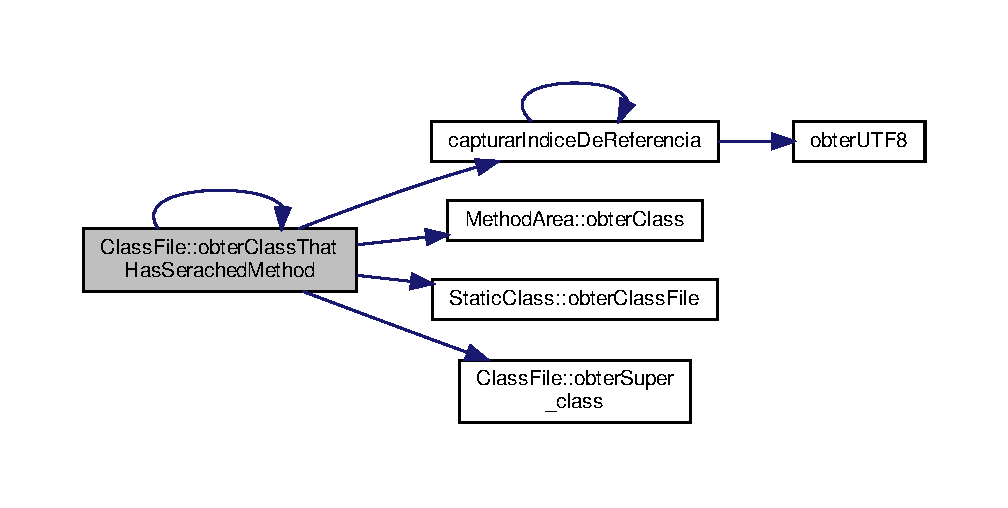
\includegraphics[width=350pt]{classClassFile_a4d0ac62c4d6218ddada33f715ebaf633_cgraph}
\end{center}
\end{figure}
\mbox{\Hypertarget{classClassFile_a1141f5a8c856d5f3931f0b518e219f79}\label{classClassFile_a1141f5a8c856d5f3931f0b518e219f79}} 
\index{Class\+File@{Class\+File}!obter\+Clinit@{obter\+Clinit}}
\index{obter\+Clinit@{obter\+Clinit}!Class\+File@{Class\+File}}
\subsubsection{\texorpdfstring{obter\+Clinit()}{obterClinit()}}
{\footnotesize\ttfamily method\+\_\+info Class\+File\+::obter\+Clinit (\begin{DoxyParamCaption}{ }\end{DoxyParamCaption})}



Retorna o método clinit. 

\begin{DoxyReturn}{Retorna}
struct method\+\_\+info contendo informações sobre o método 
\end{DoxyReturn}


Definido na linha 358 do ficheiro Class\+File.\+cpp.



Referências clinit e methods.



Referenciado por Method\+Area\+::adicionar\+Classe().

\mbox{\Hypertarget{classClassFile_ab70fe581c4b7a1824adf490c3a53bcc7}\label{classClassFile_ab70fe581c4b7a1824adf490c3a53bcc7}} 
\index{Class\+File@{Class\+File}!obter\+Constant\+Pool@{obter\+Constant\+Pool}}
\index{obter\+Constant\+Pool@{obter\+Constant\+Pool}!Class\+File@{Class\+File}}
\subsubsection{\texorpdfstring{obter\+Constant\+Pool()}{obterConstantPool()}}
{\footnotesize\ttfamily cp\+\_\+info $\ast$ Class\+File\+::obter\+Constant\+Pool (\begin{DoxyParamCaption}{ }\end{DoxyParamCaption}) const}



Retorna referencia a constant pool. 

\begin{DoxyReturn}{Retorna}
Retorna a array com a constant pool 
\end{DoxyReturn}


Definido na linha 441 do ficheiro Class\+File.\+cpp.



Referências constant\+Pool.



Referenciado por Method\+Area\+::adicionar\+Classe(), Instance\+Class\+::\+Instance\+Class(), Operations\+::invokeinterface(), Operations\+::invokespecial(), Operations\+::invokestatic(), Operations\+::invokevirtual(), Operations\+::obter\+Static\+Class\+That\+Has\+Field(), Pilha\+J\+V\+M\+::\+Pilha\+J\+V\+M() e Static\+Class\+::\+Static\+Class().

\mbox{\Hypertarget{classClassFile_a32767b8d966ef87249aa3a41ec5d67c3}\label{classClassFile_a32767b8d966ef87249aa3a41ec5d67c3}} 
\index{Class\+File@{Class\+File}!obter\+Erro@{obter\+Erro}}
\index{obter\+Erro@{obter\+Erro}!Class\+File@{Class\+File}}
\subsubsection{\texorpdfstring{obter\+Erro()}{obterErro()}}
{\footnotesize\ttfamily string Class\+File\+::obter\+Erro (\begin{DoxyParamCaption}\item[{int}]{erro }\end{DoxyParamCaption})\hspace{0.3cm}{\ttfamily [private]}}



Retorna a string que contém uma mensagem de erro correspondente ao índice que recebe como parâmetro. 


\begin{DoxyParams}{Parâmetros}
{\em erro} & M\+A\+C\+RO com o erro que foi encontrado \\
\hline
\end{DoxyParams}
\begin{DoxyReturn}{Retorna}
string contendo informação sobre o tipo de erro encontrado 
\end{DoxyReturn}


Definido na linha 408 do ficheiro Class\+File.\+cpp.



Referências C\+A\+N\+T\+\_\+\+O\+P\+EN, file\+Name, I\+N\+V\+A\+L\+I\+D\+\_\+\+E\+X\+T\+E\+N\+S\+I\+ON, I\+N\+V\+A\+L\+I\+D\+\_\+\+F\+I\+LE, I\+N\+V\+A\+L\+I\+D\+\_\+\+N\+A\+ME, M\+I\+S\+S\+I\+N\+G\+\_\+\+A\+R\+G\+U\+M\+E\+NT, M\+I\+S\+S\+I\+N\+G\+\_\+\+C\+L\+I\+N\+IT, M\+I\+S\+S\+I\+N\+G\+\_\+\+M\+A\+IN e U\+N\+K\+N\+O\+W\+N\+\_\+\+T\+Y\+PE.



Referenciado por carregar() e validacao().

\mbox{\Hypertarget{classClassFile_a1ae90b1662ca222c9910c14997b20eaa}\label{classClassFile_a1ae90b1662ca222c9910c14997b20eaa}} 
\index{Class\+File@{Class\+File}!obter\+Field@{obter\+Field}}
\index{obter\+Field@{obter\+Field}!Class\+File@{Class\+File}}
\subsubsection{\texorpdfstring{obter\+Field()}{obterField()}}
{\footnotesize\ttfamily field\+\_\+info $\ast$ Class\+File\+::obter\+Field (\begin{DoxyParamCaption}\item[{string}]{nome }\end{DoxyParamCaption})}



Retorna um field. 


\begin{DoxyParams}{Parâmetros}
{\em nome} & do field desejado que deseja retornar \\
\hline
\end{DoxyParams}
\begin{DoxyReturn}{Retorna}
struct field\+\_\+info com a informação da field passada no parâmetro 
\end{DoxyReturn}


Definido na linha 504 do ficheiro Class\+File.\+cpp.



Referências capturar\+Indice\+De\+Referencia(), constant\+Pool, fields e obter\+Fields\+Count().

Grafo de chamadas desta função\+:
\nopagebreak
\begin{figure}[H]
\begin{center}
\leavevmode
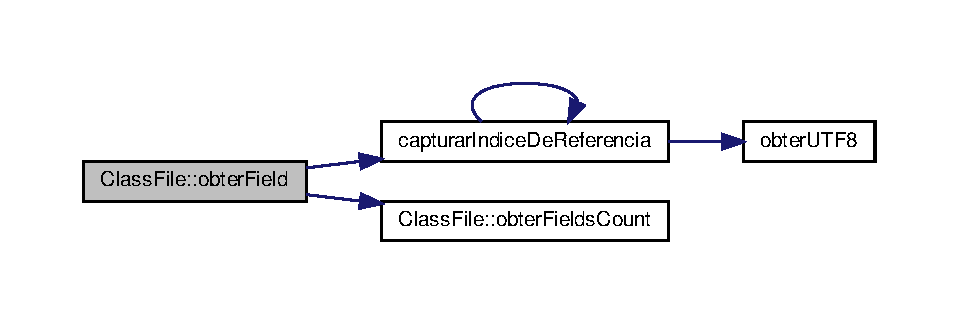
\includegraphics[width=350pt]{classClassFile_a1ae90b1662ca222c9910c14997b20eaa_cgraph}
\end{center}
\end{figure}
\mbox{\Hypertarget{classClassFile_ac3aabaa918413884416692b29165b463}\label{classClassFile_ac3aabaa918413884416692b29165b463}} 
\index{Class\+File@{Class\+File}!obter\+Fields@{obter\+Fields}}
\index{obter\+Fields@{obter\+Fields}!Class\+File@{Class\+File}}
\subsubsection{\texorpdfstring{obter\+Fields()}{obterFields()}}
{\footnotesize\ttfamily field\+\_\+info Class\+File\+::obter\+Fields (\begin{DoxyParamCaption}{ }\end{DoxyParamCaption})}



Retorna a array com as fields lidas. 

\begin{DoxyReturn}{Retorna}
a array da struct field\+\_\+info 
\end{DoxyReturn}


Definido na linha 500 do ficheiro Class\+File.\+cpp.



Referências fields.



Referenciado por Instance\+Class\+::\+Instance\+Class() e Static\+Class\+::\+Static\+Class().

\mbox{\Hypertarget{classClassFile_a0be559cd8b7b3168c81a2782e4facb0c}\label{classClassFile_a0be559cd8b7b3168c81a2782e4facb0c}} 
\index{Class\+File@{Class\+File}!obter\+Fields\+Count@{obter\+Fields\+Count}}
\index{obter\+Fields\+Count@{obter\+Fields\+Count}!Class\+File@{Class\+File}}
\subsubsection{\texorpdfstring{obter\+Fields\+Count()}{obterFieldsCount()}}
{\footnotesize\ttfamily \hyperlink{BasicTypes_8h_a90240657108b1b457eef9d3f76e0202e}{U2} Class\+File\+::obter\+Fields\+Count (\begin{DoxyParamCaption}{ }\end{DoxyParamCaption})}



Retorna número de fields. 

\begin{DoxyReturn}{Retorna}
uint16\+\_\+t indicando o numero de fields 
\end{DoxyReturn}


Definido na linha 496 do ficheiro Class\+File.\+cpp.



Referências fields\+Count.



Referenciado por Instance\+Class\+::\+Instance\+Class(), obter\+Field() e Static\+Class\+::\+Static\+Class().

\mbox{\Hypertarget{classClassFile_afdbe9cc2f360e04273470202c4f247dc}\label{classClassFile_afdbe9cc2f360e04273470202c4f247dc}} 
\index{Class\+File@{Class\+File}!obter\+Main@{obter\+Main}}
\index{obter\+Main@{obter\+Main}!Class\+File@{Class\+File}}
\subsubsection{\texorpdfstring{obter\+Main()}{obterMain()}}
{\footnotesize\ttfamily method\+\_\+info Class\+File\+::obter\+Main (\begin{DoxyParamCaption}{ }\end{DoxyParamCaption})}



Retorna o método main. 

\begin{DoxyReturn}{Retorna}
struct method\+\_\+info contendo informações sobre o método 
\end{DoxyReturn}


Definido na linha 350 do ficheiro Class\+File.\+cpp.



Referências encontrou\+Main, main\+Method e methods.



Referenciado por Pilha\+J\+V\+M\+::\+Pilha\+J\+V\+M().

\mbox{\Hypertarget{classClassFile_aac49e7e39f677987b53fdf15787b8106}\label{classClassFile_aac49e7e39f677987b53fdf15787b8106}} 
\index{Class\+File@{Class\+File}!obter\+Method@{obter\+Method}}
\index{obter\+Method@{obter\+Method}!Class\+File@{Class\+File}}
\subsubsection{\texorpdfstring{obter\+Method()}{obterMethod()}}
{\footnotesize\ttfamily method\+\_\+info $\ast$ Class\+File\+::obter\+Method (\begin{DoxyParamCaption}\item[{string}]{nome,  }\item[{string}]{descriptor }\end{DoxyParamCaption})}


\begin{DoxyParams}{Parâmetros}
{\em nome} & Nome do method desejado \\
\hline
{\em descriptor} & Descritor do method desejado \\
\hline
\end{DoxyParams}


Definido na linha 515 do ficheiro Class\+File.\+cpp.



Referências capturar\+Indice\+De\+Referencia(), constant\+Pool, Method\+\_\+info\+::descriptor\+\_\+index, methods, methods\+Count, Method\+\_\+info\+::name\+\_\+index, Method\+Area\+::obter\+Class(), Static\+Class\+::obter\+Class\+File(), obter\+Method() e obter\+Super\+\_\+class().



Referenciado por Operations\+::invokeinterface(), Operations\+::invokespecial(), Operations\+::invokestatic(), Operations\+::invokevirtual() e obter\+Method().

Grafo de chamadas desta função\+:
\nopagebreak
\begin{figure}[H]
\begin{center}
\leavevmode
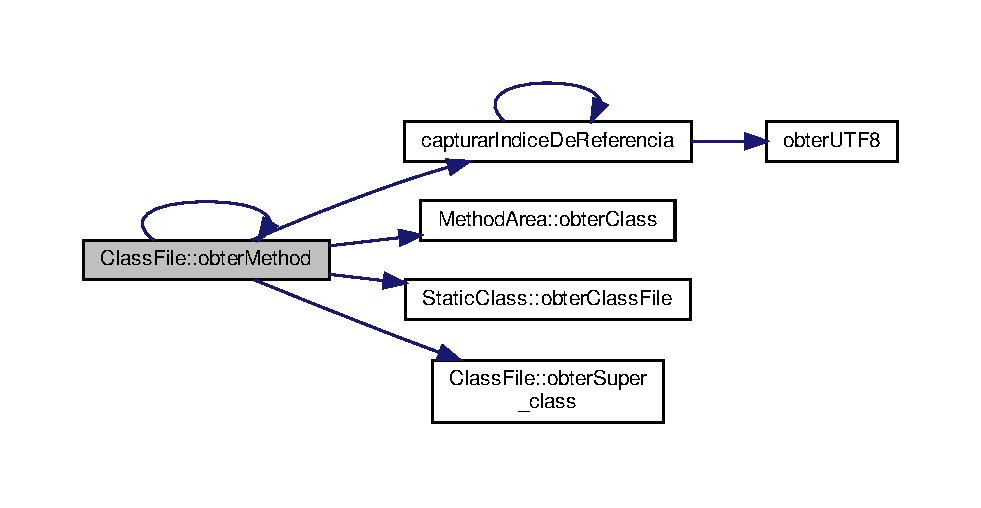
\includegraphics[width=350pt]{classClassFile_aac49e7e39f677987b53fdf15787b8106_cgraph}
\end{center}
\end{figure}
\mbox{\Hypertarget{classClassFile_a6ecce8d87f74c84b07f102c0298de13a}\label{classClassFile_a6ecce8d87f74c84b07f102c0298de13a}} 
\index{Class\+File@{Class\+File}!obter\+Methods@{obter\+Methods}}
\index{obter\+Methods@{obter\+Methods}!Class\+File@{Class\+File}}
\subsubsection{\texorpdfstring{obter\+Methods()}{obterMethods()}}
{\footnotesize\ttfamily method\+\_\+info $\ast$ Class\+File\+::obter\+Methods (\begin{DoxyParamCaption}{ }\end{DoxyParamCaption})}



Retorna todos os métodos. 

\begin{DoxyReturn}{Retorna}
array do tipo method\+\_\+info 
\end{DoxyReturn}


Definido na linha 480 do ficheiro Class\+File.\+cpp.



Referências methods.

\mbox{\Hypertarget{classClassFile_a16409bc8b58eb4965a1e39497cc300d8}\label{classClassFile_a16409bc8b58eb4965a1e39497cc300d8}} 
\index{Class\+File@{Class\+File}!obter\+Methods\+Count@{obter\+Methods\+Count}}
\index{obter\+Methods\+Count@{obter\+Methods\+Count}!Class\+File@{Class\+File}}
\subsubsection{\texorpdfstring{obter\+Methods\+Count()}{obterMethodsCount()}}
{\footnotesize\ttfamily \hyperlink{BasicTypes_8h_a90240657108b1b457eef9d3f76e0202e}{U2} Class\+File\+::obter\+Methods\+Count (\begin{DoxyParamCaption}{ }\end{DoxyParamCaption})}



Retorna o numero de Methods. 

\begin{DoxyReturn}{Retorna}
uint16\+\_\+t indicando o numero de metodos 
\end{DoxyReturn}


Definido na linha 484 do ficheiro Class\+File.\+cpp.



Referências methods\+Count.

\mbox{\Hypertarget{classClassFile_a4803bd3f325fbab1bf9c0f774b3a8c97}\label{classClassFile_a4803bd3f325fbab1bf9c0f774b3a8c97}} 
\index{Class\+File@{Class\+File}!obter\+Path@{obter\+Path}}
\index{obter\+Path@{obter\+Path}!Class\+File@{Class\+File}}
\subsubsection{\texorpdfstring{obter\+Path()}{obterPath()}}
{\footnotesize\ttfamily char $\ast$ Class\+File\+::obter\+Path (\begin{DoxyParamCaption}{ }\end{DoxyParamCaption})}



Pega o caminho do arquivo .class. 

\begin{DoxyReturn}{Retorna}
Retorna a string com o caminho total do arquivo 
\end{DoxyReturn}


Definido na linha 449 do ficheiro Class\+File.\+cpp.



Referências file\+Name.



Referenciado por main().

\mbox{\Hypertarget{classClassFile_a170339cd16cf0afc0567865b3f372d38}\label{classClassFile_a170339cd16cf0afc0567865b3f372d38}} 
\index{Class\+File@{Class\+File}!obter\+Status@{obter\+Status}}
\index{obter\+Status@{obter\+Status}!Class\+File@{Class\+File}}
\subsubsection{\texorpdfstring{obter\+Status()}{obterStatus()}}
{\footnotesize\ttfamily int Class\+File\+::obter\+Status (\begin{DoxyParamCaption}{ }\end{DoxyParamCaption})}



Retorna o status lido, informando para o método que chamou o que aconteceu. 

\begin{DoxyReturn}{Retorna}
status 
\end{DoxyReturn}


Definido na linha 404 do ficheiro Class\+File.\+cpp.



Referências status.



Referenciado por Method\+Area\+::adicionar\+Classe() e main().

\mbox{\Hypertarget{classClassFile_a8f248001f388181db10e76602031d560}\label{classClassFile_a8f248001f388181db10e76602031d560}} 
\index{Class\+File@{Class\+File}!obter\+Super\+\_\+class@{obter\+Super\+\_\+class}}
\index{obter\+Super\+\_\+class@{obter\+Super\+\_\+class}!Class\+File@{Class\+File}}
\subsubsection{\texorpdfstring{obter\+Super\+\_\+class()}{obterSuper\_class()}}
{\footnotesize\ttfamily \hyperlink{BasicTypes_8h_a90240657108b1b457eef9d3f76e0202e}{U2} Class\+File\+::obter\+Super\+\_\+class (\begin{DoxyParamCaption}{ }\end{DoxyParamCaption})}



Retorna um índice da constant pool que aponta para string com nome da superclass. 

\begin{DoxyReturn}{Retorna}
uint16\+\_\+t super\+\_\+class 
\end{DoxyReturn}


Definido na linha 492 do ficheiro Class\+File.\+cpp.



Referências super\+\_\+class.



Referenciado por obter\+Class\+That\+Has\+Serached\+Method(), obter\+Method() e Operations\+::obter\+Static\+Class\+That\+Has\+Field().

\mbox{\Hypertarget{classClassFile_a8b60418144c498b9d9545b1784bddf21}\label{classClassFile_a8b60418144c498b9d9545b1784bddf21}} 
\index{Class\+File@{Class\+File}!obter\+Tamanho\+Constant\+Pool@{obter\+Tamanho\+Constant\+Pool}}
\index{obter\+Tamanho\+Constant\+Pool@{obter\+Tamanho\+Constant\+Pool}!Class\+File@{Class\+File}}
\subsubsection{\texorpdfstring{obter\+Tamanho\+Constant\+Pool()}{obterTamanhoConstantPool()}}
{\footnotesize\ttfamily \hyperlink{BasicTypes_8h_a90240657108b1b457eef9d3f76e0202e}{U2} Class\+File\+::obter\+Tamanho\+Constant\+Pool (\begin{DoxyParamCaption}{ }\end{DoxyParamCaption})}



Retorna o valor do tamanho da constant pool. 

\begin{DoxyReturn}{Retorna}
Retorna a array com a constant pool 
\end{DoxyReturn}


Definido na linha 445 do ficheiro Class\+File.\+cpp.



Referências length\+CP.

\mbox{\Hypertarget{classClassFile_aec88c5432526d16b546ed59e5cec2136}\label{classClassFile_aec88c5432526d16b546ed59e5cec2136}} 
\index{Class\+File@{Class\+File}!obter\+This\+\_\+class@{obter\+This\+\_\+class}}
\index{obter\+This\+\_\+class@{obter\+This\+\_\+class}!Class\+File@{Class\+File}}
\subsubsection{\texorpdfstring{obter\+This\+\_\+class()}{obterThis\_class()}}
{\footnotesize\ttfamily \hyperlink{BasicTypes_8h_a90240657108b1b457eef9d3f76e0202e}{U2} Class\+File\+::obter\+This\+\_\+class (\begin{DoxyParamCaption}{ }\end{DoxyParamCaption})}



Retorna um índice da constant pool que aponta para string com nome da class. 

\begin{DoxyReturn}{Retorna}
uint16\+\_\+t this\+\_\+class 
\end{DoxyReturn}


Definido na linha 488 do ficheiro Class\+File.\+cpp.



Referências this\+\_\+class.



Referenciado por Method\+Area\+::adicionar\+Classe().

\mbox{\Hypertarget{classClassFile_acdb7018a6926b187bc6ecc18abf0fff8}\label{classClassFile_acdb7018a6926b187bc6ecc18abf0fff8}} 
\index{Class\+File@{Class\+File}!validacao@{validacao}}
\index{validacao@{validacao}!Class\+File@{Class\+File}}
\subsubsection{\texorpdfstring{validacao()}{validacao()}}
{\footnotesize\ttfamily Class\+File\+::validacao (\begin{DoxyParamCaption}\item[{void}]{ }\end{DoxyParamCaption})}



Valida estrutura obrigatoria. 



Definido na linha 45 do ficheiro Class\+File.\+cpp.



Referências I\+N\+V\+A\+L\+I\+D\+\_\+\+E\+X\+T\+E\+N\+S\+I\+ON, I\+N\+V\+A\+L\+I\+D\+\_\+\+N\+A\+ME, M\+I\+S\+S\+I\+N\+G\+\_\+\+M\+A\+IN, obter\+Erro(), status, validar\+Extensao(), verificar\+Main() e verificar\+This\+Class().



Referenciado por main().

Grafo de chamadas desta função\+:
\nopagebreak
\begin{figure}[H]
\begin{center}
\leavevmode
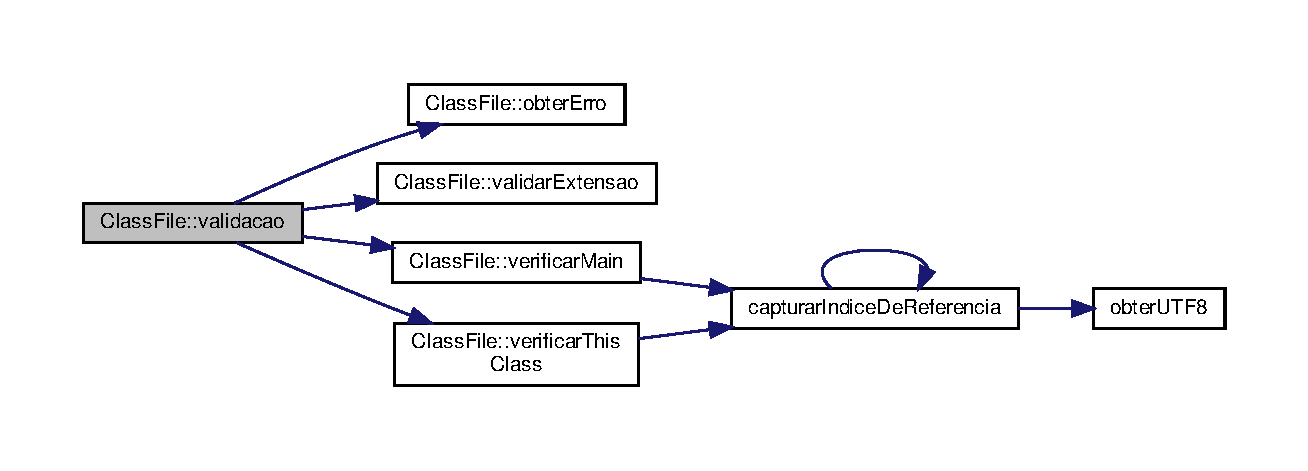
\includegraphics[width=350pt]{classClassFile_acdb7018a6926b187bc6ecc18abf0fff8_cgraph}
\end{center}
\end{figure}
\mbox{\Hypertarget{classClassFile_a8dd042ff6873b9f0d16f8ee3812261e1}\label{classClassFile_a8dd042ff6873b9f0d16f8ee3812261e1}} 
\index{Class\+File@{Class\+File}!validar\+Extensao@{validar\+Extensao}}
\index{validar\+Extensao@{validar\+Extensao}!Class\+File@{Class\+File}}
\subsubsection{\texorpdfstring{validar\+Extensao()}{validarExtensao()}}
{\footnotesize\ttfamily bool Class\+File\+::validar\+Extensao (\begin{DoxyParamCaption}{ }\end{DoxyParamCaption})}



Verifica se a extensão do arquivo é .class. 

\begin{DoxyReturn}{Retorna}
booleano que indica se existe o .class 
\end{DoxyReturn}


Definido na linha 284 do ficheiro Class\+File.\+cpp.



Referências file\+Name.



Referenciado por Method\+Area\+::adicionar\+Classe(), carregar() e validacao().

\mbox{\Hypertarget{classClassFile_ab0394185a299f35a9b5be68143385e84}\label{classClassFile_ab0394185a299f35a9b5be68143385e84}} 
\index{Class\+File@{Class\+File}!verificar\+Clinit@{verificar\+Clinit}}
\index{verificar\+Clinit@{verificar\+Clinit}!Class\+File@{Class\+File}}
\subsubsection{\texorpdfstring{verificar\+Clinit()}{verificarClinit()}}
{\footnotesize\ttfamily bool Class\+File\+::verificar\+Clinit (\begin{DoxyParamCaption}{ }\end{DoxyParamCaption})\hspace{0.3cm}{\ttfamily [private]}}



Encontra em qual method esta a clinit, se existir. 

\begin{DoxyReturn}{Retorna}
booleano que indica se existe o metodo clinit 
\end{DoxyReturn}


Definido na linha 320 do ficheiro Class\+File.\+cpp.



Referências capturar\+Indice\+De\+Referencia(), clinit, constant\+Pool, methods, methods\+Count e Method\+\_\+info\+::name\+\_\+index.



Referenciado por carregar() e existe\+Clinit().

Grafo de chamadas desta função\+:
\nopagebreak
\begin{figure}[H]
\begin{center}
\leavevmode
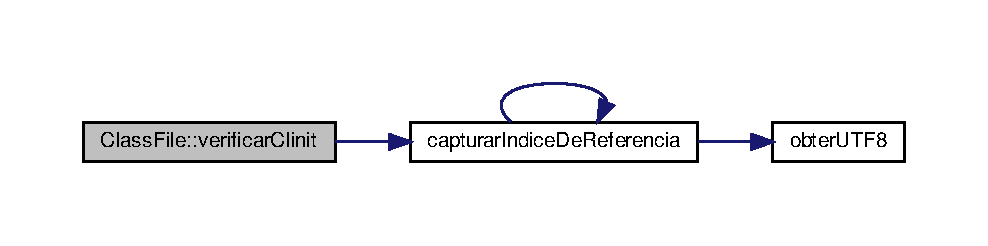
\includegraphics[width=350pt]{classClassFile_ab0394185a299f35a9b5be68143385e84_cgraph}
\end{center}
\end{figure}
\mbox{\Hypertarget{classClassFile_ae8e4445e763c4ee7c04995fcea0369e0}\label{classClassFile_ae8e4445e763c4ee7c04995fcea0369e0}} 
\index{Class\+File@{Class\+File}!verificar\+Main@{verificar\+Main}}
\index{verificar\+Main@{verificar\+Main}!Class\+File@{Class\+File}}
\subsubsection{\texorpdfstring{verificar\+Main()}{verificarMain()}}
{\footnotesize\ttfamily bool Class\+File\+::verificar\+Main (\begin{DoxyParamCaption}{ }\end{DoxyParamCaption})\hspace{0.3cm}{\ttfamily [private]}}



Encontro em qual method está a main. 

\begin{DoxyReturn}{Retorna}
booleano que indica se existe o metodo main 
\end{DoxyReturn}


Definido na linha 297 do ficheiro Class\+File.\+cpp.



Referências Method\+\_\+info\+::access\+\_\+flags, capturar\+Indice\+De\+Referencia(), constant\+Pool, Method\+\_\+info\+::descriptor\+\_\+index, main\+Method, methods, methods\+Count e Method\+\_\+info\+::name\+\_\+index.



Referenciado por carregar(), existe\+Main() e validacao().

Grafo de chamadas desta função\+:
\nopagebreak
\begin{figure}[H]
\begin{center}
\leavevmode
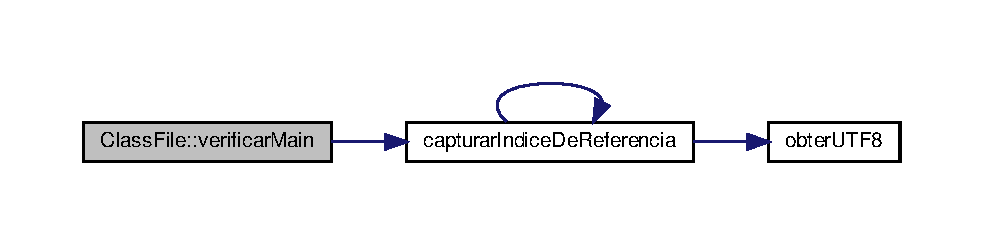
\includegraphics[width=350pt]{classClassFile_ae8e4445e763c4ee7c04995fcea0369e0_cgraph}
\end{center}
\end{figure}
\mbox{\Hypertarget{classClassFile_a6b8f23db0ee4af80a2e75d46a191dc20}\label{classClassFile_a6b8f23db0ee4af80a2e75d46a191dc20}} 
\index{Class\+File@{Class\+File}!verificar\+This\+Class@{verificar\+This\+Class}}
\index{verificar\+This\+Class@{verificar\+This\+Class}!Class\+File@{Class\+File}}
\subsubsection{\texorpdfstring{verificar\+This\+Class()}{verificarThisClass()}}
{\footnotesize\ttfamily bool Class\+File\+::verificar\+This\+Class (\begin{DoxyParamCaption}{ }\end{DoxyParamCaption})}



Verifica se a class definida é igual ao nome da classe sem extensões. 

\begin{DoxyReturn}{Retorna}
booleano indicando se a .class está correta 
\end{DoxyReturn}


Definido na linha 362 do ficheiro Class\+File.\+cpp.



Referências capturar\+Indice\+De\+Referencia(), constant\+Pool, file\+Name e this\+\_\+class.



Referenciado por carregar() e validacao().

Grafo de chamadas desta função\+:
\nopagebreak
\begin{figure}[H]
\begin{center}
\leavevmode
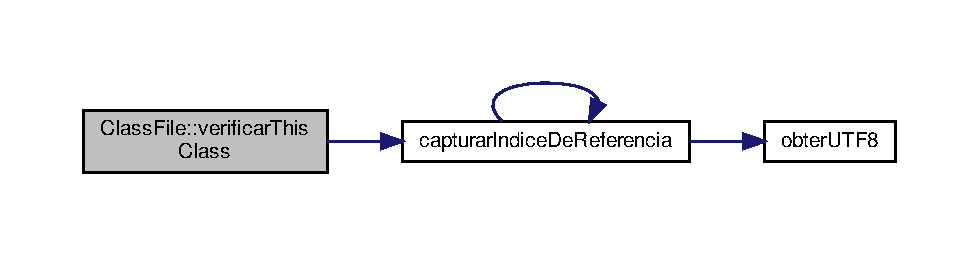
\includegraphics[width=350pt]{classClassFile_a6b8f23db0ee4af80a2e75d46a191dc20_cgraph}
\end{center}
\end{figure}


\subsection{Documentação dos dados membro}
\mbox{\Hypertarget{classClassFile_a16d2ca3e9cdf9267adde08575c57bfa9}\label{classClassFile_a16d2ca3e9cdf9267adde08575c57bfa9}} 
\index{Class\+File@{Class\+File}!access\+Flags@{access\+Flags}}
\index{access\+Flags@{access\+Flags}!Class\+File@{Class\+File}}
\subsubsection{\texorpdfstring{access\+Flags}{accessFlags}}
{\footnotesize\ttfamily \hyperlink{BasicTypes_8h_a90240657108b1b457eef9d3f76e0202e}{U2} Class\+File\+::access\+Flags\hspace{0.3cm}{\ttfamily [private]}}



Definido na linha 249 do ficheiro Class\+File.\+h.



Referenciado por carregar(), gravar\+Arquivo\+Informacoes\+Gerais() e imprimir\+Informacoes\+Gerais().

\mbox{\Hypertarget{classClassFile_ae2be12dcc1a042970b4d7d7cf9709624}\label{classClassFile_ae2be12dcc1a042970b4d7d7cf9709624}} 
\index{Class\+File@{Class\+File}!arquivo\+Class@{arquivo\+Class}}
\index{arquivo\+Class@{arquivo\+Class}!Class\+File@{Class\+File}}
\subsubsection{\texorpdfstring{arquivo\+Class}{arquivoClass}}
{\footnotesize\ttfamily F\+I\+LE$\ast$ Class\+File\+::arquivo\+Class\hspace{0.3cm}{\ttfamily [private]}}



Definido na linha 255 do ficheiro Class\+File.\+h.



Referenciado por carregar().

\mbox{\Hypertarget{classClassFile_a4aee6c7763d46884d5b2c0297142df99}\label{classClassFile_a4aee6c7763d46884d5b2c0297142df99}} 
\index{Class\+File@{Class\+File}!arquivo\+Saida@{arquivo\+Saida}}
\index{arquivo\+Saida@{arquivo\+Saida}!Class\+File@{Class\+File}}
\subsubsection{\texorpdfstring{arquivo\+Saida}{arquivoSaida}}
{\footnotesize\ttfamily fstream Class\+File\+::arquivo\+Saida\hspace{0.3cm}{\ttfamily [private]}}



Definido na linha 256 do ficheiro Class\+File.\+h.



Referenciado por fechar\+Arquivo(), gravar\+Arquivo(), gravar\+Arquivo\+Informacoes\+Gerais() e inicializar\+Arquivo().

\mbox{\Hypertarget{classClassFile_a20d4b18030becbd8df5b7584477e94b6}\label{classClassFile_a20d4b18030becbd8df5b7584477e94b6}} 
\index{Class\+File@{Class\+File}!attributes@{attributes}}
\index{attributes@{attributes}!Class\+File@{Class\+File}}
\subsubsection{\texorpdfstring{attributes}{attributes}}
{\footnotesize\ttfamily \hyperlink{structAttribute__info}{Attribute\+\_\+info}$\ast$ Class\+File\+::attributes\hspace{0.3cm}{\ttfamily [private]}}



Definido na linha 254 do ficheiro Class\+File.\+h.



Referenciado por carregar(), exibir() e gravar\+Arquivo().

\mbox{\Hypertarget{classClassFile_a66691e77df3f8604eebebc8759953542}\label{classClassFile_a66691e77df3f8604eebebc8759953542}} 
\index{Class\+File@{Class\+File}!attributes\+Count@{attributes\+Count}}
\index{attributes\+Count@{attributes\+Count}!Class\+File@{Class\+File}}
\subsubsection{\texorpdfstring{attributes\+Count}{attributesCount}}
{\footnotesize\ttfamily \hyperlink{BasicTypes_8h_a90240657108b1b457eef9d3f76e0202e}{U2} Class\+File\+::attributes\+Count\hspace{0.3cm}{\ttfamily [private]}}



Definido na linha 249 do ficheiro Class\+File.\+h.



Referenciado por carregar(), exibir(), gravar\+Arquivo(), gravar\+Arquivo\+Informacoes\+Gerais() e imprimir\+Informacoes\+Gerais().

\mbox{\Hypertarget{classClassFile_aa1eb77ebbd737bde7edde5fbdb2b6992}\label{classClassFile_aa1eb77ebbd737bde7edde5fbdb2b6992}} 
\index{Class\+File@{Class\+File}!clinit@{clinit}}
\index{clinit@{clinit}!Class\+File@{Class\+File}}
\subsubsection{\texorpdfstring{clinit}{clinit}}
{\footnotesize\ttfamily int Class\+File\+::clinit\hspace{0.3cm}{\ttfamily [private]}}



Definido na linha 244 do ficheiro Class\+File.\+h.



Referenciado por obter\+Clinit() e verificar\+Clinit().

\mbox{\Hypertarget{classClassFile_a5883215e48e253a84c105a18d34049ca}\label{classClassFile_a5883215e48e253a84c105a18d34049ca}} 
\index{Class\+File@{Class\+File}!constant\+Pool@{constant\+Pool}}
\index{constant\+Pool@{constant\+Pool}!Class\+File@{Class\+File}}
\subsubsection{\texorpdfstring{constant\+Pool}{constantPool}}
{\footnotesize\ttfamily \hyperlink{structCp__info}{Cp\+\_\+info}$\ast$ Class\+File\+::constant\+Pool\hspace{0.3cm}{\ttfamily [private]}}



Definido na linha 251 do ficheiro Class\+File.\+h.



Referenciado por carregar(), exibir(), gravar\+Arquivo(), gravar\+Arquivo\+Informacoes\+Gerais(), imprimir\+Informacoes\+Gerais(), obter\+Class\+That\+Has\+Serached\+Method(), obter\+Constant\+Pool(), obter\+Field(), obter\+Method(), verificar\+Clinit(), verificar\+Main() e verificar\+This\+Class().

\mbox{\Hypertarget{classClassFile_a5c60c8d51584f48f22bdbdd719960e05}\label{classClassFile_a5c60c8d51584f48f22bdbdd719960e05}} 
\index{Class\+File@{Class\+File}!encontrou\+Clinit@{encontrou\+Clinit}}
\index{encontrou\+Clinit@{encontrou\+Clinit}!Class\+File@{Class\+File}}
\subsubsection{\texorpdfstring{encontrou\+Clinit}{encontrouClinit}}
{\footnotesize\ttfamily bool Class\+File\+::encontrou\+Clinit\hspace{0.3cm}{\ttfamily [private]}}



Definido na linha 245 do ficheiro Class\+File.\+h.



Referenciado por carregar() e existe\+Clinit().

\mbox{\Hypertarget{classClassFile_ad8d08e096c470901c62d1a9e31a202bf}\label{classClassFile_ad8d08e096c470901c62d1a9e31a202bf}} 
\index{Class\+File@{Class\+File}!encontrou\+Main@{encontrou\+Main}}
\index{encontrou\+Main@{encontrou\+Main}!Class\+File@{Class\+File}}
\subsubsection{\texorpdfstring{encontrou\+Main}{encontrouMain}}
{\footnotesize\ttfamily bool Class\+File\+::encontrou\+Main\hspace{0.3cm}{\ttfamily [private]}}



Definido na linha 245 do ficheiro Class\+File.\+h.



Referenciado por carregar(), existe\+Main() e obter\+Main().

\mbox{\Hypertarget{classClassFile_a6d6ec8aa668982ea722edc40b3ea5b1a}\label{classClassFile_a6d6ec8aa668982ea722edc40b3ea5b1a}} 
\index{Class\+File@{Class\+File}!fields@{fields}}
\index{fields@{fields}!Class\+File@{Class\+File}}
\subsubsection{\texorpdfstring{fields}{fields}}
{\footnotesize\ttfamily \hyperlink{structField__info}{Field\+\_\+info}$\ast$ Class\+File\+::fields\hspace{0.3cm}{\ttfamily [private]}}



Definido na linha 252 do ficheiro Class\+File.\+h.



Referenciado por carregar(), exibir(), gravar\+Arquivo(), obter\+Field() e obter\+Fields().

\mbox{\Hypertarget{classClassFile_a5eae2e906695e596b89614df0e4b060a}\label{classClassFile_a5eae2e906695e596b89614df0e4b060a}} 
\index{Class\+File@{Class\+File}!fields\+Count@{fields\+Count}}
\index{fields\+Count@{fields\+Count}!Class\+File@{Class\+File}}
\subsubsection{\texorpdfstring{fields\+Count}{fieldsCount}}
{\footnotesize\ttfamily \hyperlink{BasicTypes_8h_a90240657108b1b457eef9d3f76e0202e}{U2} Class\+File\+::fields\+Count\hspace{0.3cm}{\ttfamily [private]}}



Definido na linha 248 do ficheiro Class\+File.\+h.



Referenciado por carregar(), exibir(), gravar\+Arquivo(), gravar\+Arquivo\+Informacoes\+Gerais(), imprimir\+Informacoes\+Gerais() e obter\+Fields\+Count().

\mbox{\Hypertarget{classClassFile_a2789cf19be5abaeadf96f83de33174a4}\label{classClassFile_a2789cf19be5abaeadf96f83de33174a4}} 
\index{Class\+File@{Class\+File}!file\+Name@{file\+Name}}
\index{file\+Name@{file\+Name}!Class\+File@{Class\+File}}
\subsubsection{\texorpdfstring{file\+Name}{fileName}}
{\footnotesize\ttfamily char$\ast$ Class\+File\+::file\+Name\hspace{0.3cm}{\ttfamily [private]}}



Definido na linha 246 do ficheiro Class\+File.\+h.



Referenciado por carregar(), Class\+File(), obter\+Erro(), obter\+Path(), validar\+Extensao() e verificar\+This\+Class().

\mbox{\Hypertarget{classClassFile_a94d1e4e835476f47e3a8b81ecd0301c0}\label{classClassFile_a94d1e4e835476f47e3a8b81ecd0301c0}} 
\index{Class\+File@{Class\+File}!interfaces@{interfaces}}
\index{interfaces@{interfaces}!Class\+File@{Class\+File}}
\subsubsection{\texorpdfstring{interfaces}{interfaces}}
{\footnotesize\ttfamily \hyperlink{BasicTypes_8h_a90240657108b1b457eef9d3f76e0202e}{U2}$\ast$ Class\+File\+::interfaces\hspace{0.3cm}{\ttfamily [private]}}



Definido na linha 250 do ficheiro Class\+File.\+h.



Referenciado por carregar(), exibir() e gravar\+Arquivo().

\mbox{\Hypertarget{classClassFile_a1bbca13f93ec21beffa8a56e360c9f8d}\label{classClassFile_a1bbca13f93ec21beffa8a56e360c9f8d}} 
\index{Class\+File@{Class\+File}!interfaces\+Count@{interfaces\+Count}}
\index{interfaces\+Count@{interfaces\+Count}!Class\+File@{Class\+File}}
\subsubsection{\texorpdfstring{interfaces\+Count}{interfacesCount}}
{\footnotesize\ttfamily \hyperlink{BasicTypes_8h_a90240657108b1b457eef9d3f76e0202e}{U2} Class\+File\+::interfaces\+Count\hspace{0.3cm}{\ttfamily [private]}}



Definido na linha 248 do ficheiro Class\+File.\+h.



Referenciado por carregar(), exibir(), gravar\+Arquivo(), gravar\+Arquivo\+Informacoes\+Gerais() e imprimir\+Informacoes\+Gerais().

\mbox{\Hypertarget{classClassFile_acde5006251ffd25149efa4d6fb725cf5}\label{classClassFile_acde5006251ffd25149efa4d6fb725cf5}} 
\index{Class\+File@{Class\+File}!length\+CP@{length\+CP}}
\index{length\+CP@{length\+CP}!Class\+File@{Class\+File}}
\subsubsection{\texorpdfstring{length\+CP}{lengthCP}}
{\footnotesize\ttfamily \hyperlink{BasicTypes_8h_a90240657108b1b457eef9d3f76e0202e}{U2} Class\+File\+::length\+CP\hspace{0.3cm}{\ttfamily [private]}}



Definido na linha 247 do ficheiro Class\+File.\+h.



Referenciado por carregar(), exibir(), gravar\+Arquivo(), gravar\+Arquivo\+Informacoes\+Gerais(), imprimir\+Informacoes\+Gerais() e obter\+Tamanho\+Constant\+Pool().

\mbox{\Hypertarget{classClassFile_ac1cdef340faa0bd945b2236057433978}\label{classClassFile_ac1cdef340faa0bd945b2236057433978}} 
\index{Class\+File@{Class\+File}!main\+Method@{main\+Method}}
\index{main\+Method@{main\+Method}!Class\+File@{Class\+File}}
\subsubsection{\texorpdfstring{main\+Method}{mainMethod}}
{\footnotesize\ttfamily int Class\+File\+::main\+Method\hspace{0.3cm}{\ttfamily [private]}}



Definido na linha 244 do ficheiro Class\+File.\+h.



Referenciado por obter\+Main() e verificar\+Main().

\mbox{\Hypertarget{classClassFile_a40bd108a13debb86701cf31742572686}\label{classClassFile_a40bd108a13debb86701cf31742572686}} 
\index{Class\+File@{Class\+File}!maj\+Version@{maj\+Version}}
\index{maj\+Version@{maj\+Version}!Class\+File@{Class\+File}}
\subsubsection{\texorpdfstring{maj\+Version}{majVersion}}
{\footnotesize\ttfamily \hyperlink{BasicTypes_8h_a90240657108b1b457eef9d3f76e0202e}{U2} Class\+File\+::maj\+Version\hspace{0.3cm}{\ttfamily [private]}}



Definido na linha 247 do ficheiro Class\+File.\+h.



Referenciado por carregar(), gravar\+Arquivo\+Informacoes\+Gerais() e imprimir\+Informacoes\+Gerais().

\mbox{\Hypertarget{classClassFile_a5906980e6c5121e5a864346fd3617083}\label{classClassFile_a5906980e6c5121e5a864346fd3617083}} 
\index{Class\+File@{Class\+File}!methods@{methods}}
\index{methods@{methods}!Class\+File@{Class\+File}}
\subsubsection{\texorpdfstring{methods}{methods}}
{\footnotesize\ttfamily \hyperlink{structMethod__info}{Method\+\_\+info}$\ast$ Class\+File\+::methods\hspace{0.3cm}{\ttfamily [private]}}



Definido na linha 253 do ficheiro Class\+File.\+h.



Referenciado por carregar(), exibir(), gravar\+Arquivo(), obter\+Class\+That\+Has\+Serached\+Method(), obter\+Clinit(), obter\+Main(), obter\+Method(), obter\+Methods(), verificar\+Clinit() e verificar\+Main().

\mbox{\Hypertarget{classClassFile_a4c362d4adfeaad02f4517caf1ba58103}\label{classClassFile_a4c362d4adfeaad02f4517caf1ba58103}} 
\index{Class\+File@{Class\+File}!methods\+Count@{methods\+Count}}
\index{methods\+Count@{methods\+Count}!Class\+File@{Class\+File}}
\subsubsection{\texorpdfstring{methods\+Count}{methodsCount}}
{\footnotesize\ttfamily \hyperlink{BasicTypes_8h_a90240657108b1b457eef9d3f76e0202e}{U2} Class\+File\+::methods\+Count\hspace{0.3cm}{\ttfamily [private]}}



Definido na linha 249 do ficheiro Class\+File.\+h.



Referenciado por carregar(), exibir(), gravar\+Arquivo(), gravar\+Arquivo\+Informacoes\+Gerais(), imprimir\+Informacoes\+Gerais(), obter\+Class\+That\+Has\+Serached\+Method(), obter\+Method(), obter\+Methods\+Count(), verificar\+Clinit() e verificar\+Main().

\mbox{\Hypertarget{classClassFile_ab0d3a4474a9907dc61893d0293525b38}\label{classClassFile_ab0d3a4474a9907dc61893d0293525b38}} 
\index{Class\+File@{Class\+File}!min\+Version@{min\+Version}}
\index{min\+Version@{min\+Version}!Class\+File@{Class\+File}}
\subsubsection{\texorpdfstring{min\+Version}{minVersion}}
{\footnotesize\ttfamily \hyperlink{BasicTypes_8h_a90240657108b1b457eef9d3f76e0202e}{U2} Class\+File\+::min\+Version\hspace{0.3cm}{\ttfamily [private]}}



Definido na linha 247 do ficheiro Class\+File.\+h.



Referenciado por carregar(), gravar\+Arquivo\+Informacoes\+Gerais() e imprimir\+Informacoes\+Gerais().

\mbox{\Hypertarget{classClassFile_a9afeae9ac0889ab75909e73933e29326}\label{classClassFile_a9afeae9ac0889ab75909e73933e29326}} 
\index{Class\+File@{Class\+File}!status@{status}}
\index{status@{status}!Class\+File@{Class\+File}}
\subsubsection{\texorpdfstring{status}{status}}
{\footnotesize\ttfamily int Class\+File\+::status\hspace{0.3cm}{\ttfamily [private]}}



Definido na linha 244 do ficheiro Class\+File.\+h.



Referenciado por carregar(), Class\+File(), exibir(), gravar\+Arquivo(), inicializar\+Arquivo(), obter\+Status() e validacao().

\mbox{\Hypertarget{classClassFile_ad92079216f8cdb366a3002e5ca2c2dfa}\label{classClassFile_ad92079216f8cdb366a3002e5ca2c2dfa}} 
\index{Class\+File@{Class\+File}!super\+\_\+class@{super\+\_\+class}}
\index{super\+\_\+class@{super\+\_\+class}!Class\+File@{Class\+File}}
\subsubsection{\texorpdfstring{super\+\_\+class}{super\_class}}
{\footnotesize\ttfamily \hyperlink{BasicTypes_8h_a90240657108b1b457eef9d3f76e0202e}{U2} Class\+File\+::super\+\_\+class\hspace{0.3cm}{\ttfamily [private]}}



Definido na linha 248 do ficheiro Class\+File.\+h.



Referenciado por carregar(), gravar\+Arquivo\+Informacoes\+Gerais(), imprimir\+Informacoes\+Gerais() e obter\+Super\+\_\+class().

\mbox{\Hypertarget{classClassFile_a205bc5af050f4676fc4c3ff7992c4959}\label{classClassFile_a205bc5af050f4676fc4c3ff7992c4959}} 
\index{Class\+File@{Class\+File}!this\+\_\+class@{this\+\_\+class}}
\index{this\+\_\+class@{this\+\_\+class}!Class\+File@{Class\+File}}
\subsubsection{\texorpdfstring{this\+\_\+class}{this\_class}}
{\footnotesize\ttfamily \hyperlink{BasicTypes_8h_a90240657108b1b457eef9d3f76e0202e}{U2} Class\+File\+::this\+\_\+class\hspace{0.3cm}{\ttfamily [private]}}



Definido na linha 248 do ficheiro Class\+File.\+h.



Referenciado por carregar(), gravar\+Arquivo\+Informacoes\+Gerais(), imprimir\+Informacoes\+Gerais(), obter\+This\+\_\+class() e verificar\+This\+Class().



A documentação para esta classe foi gerada a partir dos seguintes ficheiros\+:\begin{DoxyCompactItemize}
\item 
include/\hyperlink{ClassFile_8h}{Class\+File.\+h}\item 
src/\hyperlink{ClassFile_8cpp}{Class\+File.\+cpp}\end{DoxyCompactItemize}

\hypertarget{unionClassLoaderType}{}\section{Referência à união Class\+Loader\+Type}
\label{unionClassLoaderType}\index{Class\+Loader\+Type@{Class\+Loader\+Type}}


Estrutura de dados para armazenamento Union responsável por armazenar todos os tamanhos de variáveis utilzadas na J\+VM.  




{\ttfamily \#include $<$Basic\+Types.\+h$>$}

\subsection*{Atributos Públicos}
\begin{DoxyCompactItemize}
\item 
\hyperlink{BasicTypes_8h_a9bffe5bb2564f91cd90fb7d06848f9a8}{U1} $\ast$ \hyperlink{unionClassLoaderType_a35ae4ff3dac1fe01b69c3649e200790c}{array}
\item 
\hyperlink{BasicTypes_8h_a9bffe5bb2564f91cd90fb7d06848f9a8}{U1} \hyperlink{unionClassLoaderType_ac3612ba54bfba5c4b856dcba8db1a8a8}{u1}
\item 
\hyperlink{BasicTypes_8h_a90240657108b1b457eef9d3f76e0202e}{U2} \hyperlink{unionClassLoaderType_aaf24600dbc4afe99210fa000bdb1e6d7}{u2}
\item 
\hyperlink{BasicTypes_8h_ac6d2ba2e53dd424684ead2f40e74a8b6}{U4} \hyperlink{unionClassLoaderType_aad01cfe6aac48729f55425b67a70622e}{u4}
\end{DoxyCompactItemize}


\subsection{Descrição detalhada}
Estrutura de dados para armazenamento Union responsável por armazenar todos os tamanhos de variáveis utilzadas na J\+VM. 

Definido na linha 44 do ficheiro Basic\+Types.\+h.



\subsection{Documentação dos dados membro}
\mbox{\Hypertarget{unionClassLoaderType_a35ae4ff3dac1fe01b69c3649e200790c}\label{unionClassLoaderType_a35ae4ff3dac1fe01b69c3649e200790c}} 
\index{Class\+Loader\+Type@{Class\+Loader\+Type}!array@{array}}
\index{array@{array}!Class\+Loader\+Type@{Class\+Loader\+Type}}
\subsubsection{\texorpdfstring{array}{array}}
{\footnotesize\ttfamily \hyperlink{BasicTypes_8h_a9bffe5bb2564f91cd90fb7d06848f9a8}{U1}$\ast$ Class\+Loader\+Type\+::array}



Definido na linha 45 do ficheiro Basic\+Types.\+h.



Referenciado por carregar\+Constant\+Pool(), Operations\+::ldc() e Operations\+::ldc\+\_\+w().

\mbox{\Hypertarget{unionClassLoaderType_ac3612ba54bfba5c4b856dcba8db1a8a8}\label{unionClassLoaderType_ac3612ba54bfba5c4b856dcba8db1a8a8}} 
\index{Class\+Loader\+Type@{Class\+Loader\+Type}!u1@{u1}}
\index{u1@{u1}!Class\+Loader\+Type@{Class\+Loader\+Type}}
\subsubsection{\texorpdfstring{u1}{u1}}
{\footnotesize\ttfamily \hyperlink{BasicTypes_8h_a9bffe5bb2564f91cd90fb7d06848f9a8}{U1} Class\+Loader\+Type\+::u1}



Definido na linha 46 do ficheiro Basic\+Types.\+h.

\mbox{\Hypertarget{unionClassLoaderType_aaf24600dbc4afe99210fa000bdb1e6d7}\label{unionClassLoaderType_aaf24600dbc4afe99210fa000bdb1e6d7}} 
\index{Class\+Loader\+Type@{Class\+Loader\+Type}!u2@{u2}}
\index{u2@{u2}!Class\+Loader\+Type@{Class\+Loader\+Type}}
\subsubsection{\texorpdfstring{u2}{u2}}
{\footnotesize\ttfamily \hyperlink{BasicTypes_8h_a90240657108b1b457eef9d3f76e0202e}{U2} Class\+Loader\+Type\+::u2}



Definido na linha 47 do ficheiro Basic\+Types.\+h.



Referenciado por carregar\+Constant\+Pool(), Operations\+::getfield(), Operations\+::getstatic(), Operations\+::invokeinterface(), Operations\+::invokespecial(), Operations\+::invokestatic(), Operations\+::invokevirtual(), Operations\+::ldc(), Operations\+::ldc\+\_\+w(), Operations\+::multianewarray(), Operations\+::putfield() e Operations\+::putstatic().

\mbox{\Hypertarget{unionClassLoaderType_aad01cfe6aac48729f55425b67a70622e}\label{unionClassLoaderType_aad01cfe6aac48729f55425b67a70622e}} 
\index{Class\+Loader\+Type@{Class\+Loader\+Type}!u4@{u4}}
\index{u4@{u4}!Class\+Loader\+Type@{Class\+Loader\+Type}}
\subsubsection{\texorpdfstring{u4}{u4}}
{\footnotesize\ttfamily \hyperlink{BasicTypes_8h_ac6d2ba2e53dd424684ead2f40e74a8b6}{U4} Class\+Loader\+Type\+::u4}



Definido na linha 48 do ficheiro Basic\+Types.\+h.



Referenciado por carregar\+Constant\+Pool(), converter\+\_\+u4\+\_\+to\+\_\+float(), converter\+\_\+u4\+\_\+to\+\_\+long(), Operations\+::ldc() e Operations\+::ldc\+\_\+w().



A documentação para esta união foi gerada a partir do seguinte ficheiro\+:\begin{DoxyCompactItemize}
\item 
include/\hyperlink{BasicTypes_8h}{Basic\+Types.\+h}\end{DoxyCompactItemize}

\hypertarget{structCode__attribute}{}\section{Referência à estrutura Code\+\_\+attribute}
\label{structCode__attribute}\index{Code\+\_\+attribute@{Code\+\_\+attribute}}


{\ttfamily \#include $<$Basic\+Types.\+h$>$}



Diagrama de colaboração para Code\+\_\+attribute\+:\nopagebreak
\begin{figure}[H]
\begin{center}
\leavevmode
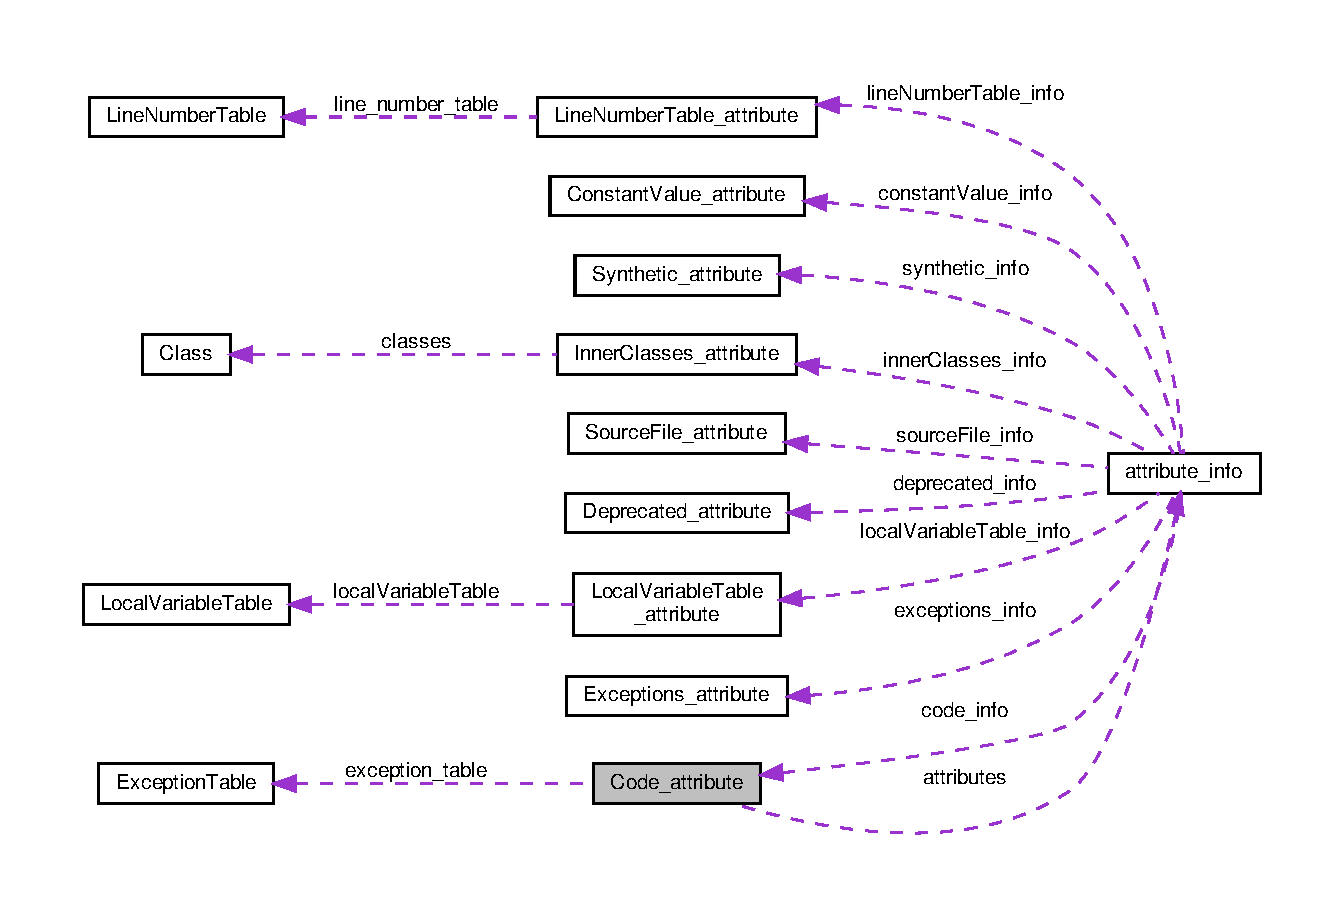
\includegraphics[width=350pt]{structCode__attribute__coll__graph}
\end{center}
\end{figure}
\subsection*{Atributos Públicos}
\begin{DoxyCompactItemize}
\item 
\hyperlink{BasicTypes_8h_a732cde1300aafb73b0ea6c2558a7a54f}{u2} \hyperlink{structCode__attribute_a300885ff1326f01f7c86e7b4425f0d35}{max\+\_\+stack}
\item 
\hyperlink{BasicTypes_8h_a732cde1300aafb73b0ea6c2558a7a54f}{u2} \hyperlink{structCode__attribute_ad710ec86a1d37c6daa999383f8f2fd35}{max\+\_\+locals}
\item 
\hyperlink{BasicTypes_8h_ae5be1f726785414dd1b77d60df074c9d}{u4} \hyperlink{structCode__attribute_a80af47e824a13ef4dc604e5b8671f793}{code\+\_\+length}
\item 
\hyperlink{BasicTypes_8h_ad9f4cdb6757615aae2fad89dab3c5470}{u1} $\ast$ \hyperlink{structCode__attribute_a26d83aeded05528b11dd486555d1ece2}{code}
\item 
\hyperlink{BasicTypes_8h_a732cde1300aafb73b0ea6c2558a7a54f}{u2} \hyperlink{structCode__attribute_a24b063ad994d77688db7468fae11e7aa}{exception\+\_\+table\+\_\+length}
\item 
\hyperlink{structExceptionTable}{Exception\+Table} $\ast$ \hyperlink{structCode__attribute_a080b3f7a5717321484a648ec83c11f12}{exception\+\_\+table}
\item 
\hyperlink{BasicTypes_8h_a732cde1300aafb73b0ea6c2558a7a54f}{u2} \hyperlink{structCode__attribute_a9ca1435aa65ae02d764ff53a36fb842f}{attributes\+\_\+count}
\item 
\hyperlink{structattribute__info}{attribute\+\_\+info} $\ast$ \hyperlink{structCode__attribute_abb5d2d93e2f165dd908c3788a323d093}{attributes}
\end{DoxyCompactItemize}


\subsection{Descrição detalhada}


Definido na linha 195 do ficheiro Basic\+Types.\+h.



\subsection{Documentação dos dados membro}
\mbox{\Hypertarget{structCode__attribute_abb5d2d93e2f165dd908c3788a323d093}\label{structCode__attribute_abb5d2d93e2f165dd908c3788a323d093}} 
\index{Code\+\_\+attribute@{Code\+\_\+attribute}!attributes@{attributes}}
\index{attributes@{attributes}!Code\+\_\+attribute@{Code\+\_\+attribute}}
\subsubsection{\texorpdfstring{attributes}{attributes}}
{\footnotesize\ttfamily \hyperlink{structattribute__info}{attribute\+\_\+info}$\ast$ Code\+\_\+attribute\+::attributes}



Definido na linha 203 do ficheiro Basic\+Types.\+h.



Referenciado por exibe\+\_\+\+Attribute\+Info(), Leitor\+Exibidor\+::get\+Attribute\+Code() e print\+\_\+\+Attribute\+Info().

\mbox{\Hypertarget{structCode__attribute_a9ca1435aa65ae02d764ff53a36fb842f}\label{structCode__attribute_a9ca1435aa65ae02d764ff53a36fb842f}} 
\index{Code\+\_\+attribute@{Code\+\_\+attribute}!attributes\+\_\+count@{attributes\+\_\+count}}
\index{attributes\+\_\+count@{attributes\+\_\+count}!Code\+\_\+attribute@{Code\+\_\+attribute}}
\subsubsection{\texorpdfstring{attributes\+\_\+count}{attributes\_count}}
{\footnotesize\ttfamily \hyperlink{BasicTypes_8h_a732cde1300aafb73b0ea6c2558a7a54f}{u2} Code\+\_\+attribute\+::attributes\+\_\+count}



Definido na linha 202 do ficheiro Basic\+Types.\+h.



Referenciado por exibe\+\_\+\+Attribute\+Info(), Leitor\+Exibidor\+::get\+Attribute\+Code() e print\+\_\+\+Attribute\+Info().

\mbox{\Hypertarget{structCode__attribute_a26d83aeded05528b11dd486555d1ece2}\label{structCode__attribute_a26d83aeded05528b11dd486555d1ece2}} 
\index{Code\+\_\+attribute@{Code\+\_\+attribute}!code@{code}}
\index{code@{code}!Code\+\_\+attribute@{Code\+\_\+attribute}}
\subsubsection{\texorpdfstring{code}{code}}
{\footnotesize\ttfamily \hyperlink{BasicTypes_8h_ad9f4cdb6757615aae2fad89dab3c5470}{u1}$\ast$ Code\+\_\+attribute\+::code}



Definido na linha 199 do ficheiro Basic\+Types.\+h.



Referenciado por exibe\+Byte\+Code(), Leitor\+Exibidor\+::get\+Attribute\+Code(), Frame\+::get\+Code() e print\+Arquivo\+Byte\+Code().

\mbox{\Hypertarget{structCode__attribute_a80af47e824a13ef4dc604e5b8671f793}\label{structCode__attribute_a80af47e824a13ef4dc604e5b8671f793}} 
\index{Code\+\_\+attribute@{Code\+\_\+attribute}!code\+\_\+length@{code\+\_\+length}}
\index{code\+\_\+length@{code\+\_\+length}!Code\+\_\+attribute@{Code\+\_\+attribute}}
\subsubsection{\texorpdfstring{code\+\_\+length}{code\_length}}
{\footnotesize\ttfamily \hyperlink{BasicTypes_8h_ae5be1f726785414dd1b77d60df074c9d}{u4} Code\+\_\+attribute\+::code\+\_\+length}



Definido na linha 198 do ficheiro Basic\+Types.\+h.



Referenciado por exibe\+\_\+\+Attribute\+Info(), exibe\+Byte\+Code(), Leitor\+Exibidor\+::get\+Attribute\+Code(), print\+\_\+\+Attribute\+Info(), print\+Arquivo\+Byte\+Code() e Frame\+::size\+Code().

\mbox{\Hypertarget{structCode__attribute_a080b3f7a5717321484a648ec83c11f12}\label{structCode__attribute_a080b3f7a5717321484a648ec83c11f12}} 
\index{Code\+\_\+attribute@{Code\+\_\+attribute}!exception\+\_\+table@{exception\+\_\+table}}
\index{exception\+\_\+table@{exception\+\_\+table}!Code\+\_\+attribute@{Code\+\_\+attribute}}
\subsubsection{\texorpdfstring{exception\+\_\+table}{exception\_table}}
{\footnotesize\ttfamily \hyperlink{structExceptionTable}{Exception\+Table}$\ast$ Code\+\_\+attribute\+::exception\+\_\+table}



Definido na linha 201 do ficheiro Basic\+Types.\+h.



Referenciado por exibe\+\_\+\+Attribute\+Info(), Leitor\+Exibidor\+::get\+Attribute\+Code() e print\+\_\+\+Attribute\+Info().

\mbox{\Hypertarget{structCode__attribute_a24b063ad994d77688db7468fae11e7aa}\label{structCode__attribute_a24b063ad994d77688db7468fae11e7aa}} 
\index{Code\+\_\+attribute@{Code\+\_\+attribute}!exception\+\_\+table\+\_\+length@{exception\+\_\+table\+\_\+length}}
\index{exception\+\_\+table\+\_\+length@{exception\+\_\+table\+\_\+length}!Code\+\_\+attribute@{Code\+\_\+attribute}}
\subsubsection{\texorpdfstring{exception\+\_\+table\+\_\+length}{exception\_table\_length}}
{\footnotesize\ttfamily \hyperlink{BasicTypes_8h_a732cde1300aafb73b0ea6c2558a7a54f}{u2} Code\+\_\+attribute\+::exception\+\_\+table\+\_\+length}



Definido na linha 200 do ficheiro Basic\+Types.\+h.



Referenciado por exibe\+\_\+\+Attribute\+Info(), Leitor\+Exibidor\+::get\+Attribute\+Code() e print\+\_\+\+Attribute\+Info().

\mbox{\Hypertarget{structCode__attribute_ad710ec86a1d37c6daa999383f8f2fd35}\label{structCode__attribute_ad710ec86a1d37c6daa999383f8f2fd35}} 
\index{Code\+\_\+attribute@{Code\+\_\+attribute}!max\+\_\+locals@{max\+\_\+locals}}
\index{max\+\_\+locals@{max\+\_\+locals}!Code\+\_\+attribute@{Code\+\_\+attribute}}
\subsubsection{\texorpdfstring{max\+\_\+locals}{max\_locals}}
{\footnotesize\ttfamily \hyperlink{BasicTypes_8h_a732cde1300aafb73b0ea6c2558a7a54f}{u2} Code\+\_\+attribute\+::max\+\_\+locals}



Definido na linha 197 do ficheiro Basic\+Types.\+h.



Referenciado por exibe\+\_\+\+Attribute\+Info(), Leitor\+Exibidor\+::get\+Attribute\+Code(), Frame\+::obter\+Local\+Variable\+Value(), print\+\_\+\+Attribute\+Info(), Frame\+::size\+Local\+Variables() e Frame\+::troca\+Local\+Variable().

\mbox{\Hypertarget{structCode__attribute_a300885ff1326f01f7c86e7b4425f0d35}\label{structCode__attribute_a300885ff1326f01f7c86e7b4425f0d35}} 
\index{Code\+\_\+attribute@{Code\+\_\+attribute}!max\+\_\+stack@{max\+\_\+stack}}
\index{max\+\_\+stack@{max\+\_\+stack}!Code\+\_\+attribute@{Code\+\_\+attribute}}
\subsubsection{\texorpdfstring{max\+\_\+stack}{max\_stack}}
{\footnotesize\ttfamily \hyperlink{BasicTypes_8h_a732cde1300aafb73b0ea6c2558a7a54f}{u2} Code\+\_\+attribute\+::max\+\_\+stack}



Definido na linha 196 do ficheiro Basic\+Types.\+h.



Referenciado por exibe\+\_\+\+Attribute\+Info(), Leitor\+Exibidor\+::get\+Attribute\+Code() e print\+\_\+\+Attribute\+Info().



A documentação para esta estrutura foi gerada a partir do seguinte ficheiro\+:\begin{DoxyCompactItemize}
\item 
include/\hyperlink{BasicTypes_8h}{Basic\+Types.\+h}\end{DoxyCompactItemize}

\hypertarget{structConstantValue__attribute}{}\section{Referência à estrutura Constant\+Value\+\_\+attribute}
\label{structConstantValue__attribute}\index{Constant\+Value\+\_\+attribute@{Constant\+Value\+\_\+attribute}}


{\ttfamily \#include $<$Basic\+Types.\+h$>$}

\subsection*{Atributos Públicos}
\begin{DoxyCompactItemize}
\item 
\hyperlink{BasicTypes_8h_a732cde1300aafb73b0ea6c2558a7a54f}{u2} \hyperlink{structConstantValue__attribute_a812157e7121906faf8018ce066d1ea27}{constantvalue\+\_\+index}
\end{DoxyCompactItemize}


\subsection{Descrição detalhada}


Definido na linha 184 do ficheiro Basic\+Types.\+h.



\subsection{Documentação dos dados membro}
\mbox{\Hypertarget{structConstantValue__attribute_a812157e7121906faf8018ce066d1ea27}\label{structConstantValue__attribute_a812157e7121906faf8018ce066d1ea27}} 
\index{Constant\+Value\+\_\+attribute@{Constant\+Value\+\_\+attribute}!constantvalue\+\_\+index@{constantvalue\+\_\+index}}
\index{constantvalue\+\_\+index@{constantvalue\+\_\+index}!Constant\+Value\+\_\+attribute@{Constant\+Value\+\_\+attribute}}
\subsubsection{\texorpdfstring{constantvalue\+\_\+index}{constantvalue\_index}}
{\footnotesize\ttfamily \hyperlink{BasicTypes_8h_a732cde1300aafb73b0ea6c2558a7a54f}{u2} Constant\+Value\+\_\+attribute\+::constantvalue\+\_\+index}



Definido na linha 185 do ficheiro Basic\+Types.\+h.



Referenciado por exibe\+\_\+\+Attribute\+Info(), Leitor\+Exibidor\+::get\+Attribute\+Constant\+Value() e print\+\_\+\+Attribute\+Info().



A documentação para esta estrutura foi gerada a partir do seguinte ficheiro\+:\begin{DoxyCompactItemize}
\item 
include/\hyperlink{BasicTypes_8h}{Basic\+Types.\+h}\end{DoxyCompactItemize}

\hypertarget{structCp__info}{}\section{Referência à estrutura Cp\+\_\+info}
\label{structCp__info}\index{Cp\+\_\+info@{Cp\+\_\+info}}


Possui um elemento pool de constante.  




{\ttfamily \#include $<$Constant\+Pool.\+h$>$}



Diagrama de colaboração para Cp\+\_\+info\+:\nopagebreak
\begin{figure}[H]
\begin{center}
\leavevmode
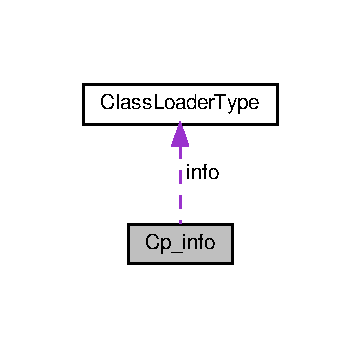
\includegraphics[width=173pt]{structCp__info__coll__graph}
\end{center}
\end{figure}
\subsection*{Atributos Públicos}
\begin{DoxyCompactItemize}
\item 
\hyperlink{BasicTypes_8h_a9bffe5bb2564f91cd90fb7d06848f9a8}{U1} \hyperlink{structCp__info_a74ba6be7ad12511cc5df37e43984add0}{tag}
\item 
\hyperlink{unionClassLoaderType}{Class\+Loader\+Type} $\ast$ \hyperlink{structCp__info_ace48d3773256ae8a504dea48352c0b93}{info}
\end{DoxyCompactItemize}


\subsection{Descrição detalhada}
Possui um elemento pool de constante. 

Definido na linha 17 do ficheiro Constant\+Pool.\+h.



\subsection{Documentação dos dados membro}
\mbox{\Hypertarget{structCp__info_ace48d3773256ae8a504dea48352c0b93}\label{structCp__info_ace48d3773256ae8a504dea48352c0b93}} 
\index{Cp\+\_\+info@{Cp\+\_\+info}!info@{info}}
\index{info@{info}!Cp\+\_\+info@{Cp\+\_\+info}}
\subsubsection{\texorpdfstring{info}{info}}
{\footnotesize\ttfamily \hyperlink{unionClassLoaderType}{Class\+Loader\+Type}$\ast$ Cp\+\_\+info\+::info}



Definido na linha 19 do ficheiro Constant\+Pool.\+h.



Referenciado por carregar\+Constant\+Pool(), Operations\+::getfield(), Operations\+::getstatic(), Operations\+::invokeinterface(), Operations\+::invokespecial(), Operations\+::invokestatic(), Operations\+::invokevirtual(), Operations\+::ldc(), Operations\+::ldc2\+\_\+w(), Operations\+::ldc\+\_\+w(), Operations\+::multianewarray(), Operations\+::putfield() e Operations\+::putstatic().

\mbox{\Hypertarget{structCp__info_a74ba6be7ad12511cc5df37e43984add0}\label{structCp__info_a74ba6be7ad12511cc5df37e43984add0}} 
\index{Cp\+\_\+info@{Cp\+\_\+info}!tag@{tag}}
\index{tag@{tag}!Cp\+\_\+info@{Cp\+\_\+info}}
\subsubsection{\texorpdfstring{tag}{tag}}
{\footnotesize\ttfamily \hyperlink{BasicTypes_8h_a9bffe5bb2564f91cd90fb7d06848f9a8}{U1} Cp\+\_\+info\+::tag}



Definido na linha 18 do ficheiro Constant\+Pool.\+h.



Referenciado por carregar\+Constant\+Pool(), Operations\+::getstatic(), gravar\+Arquivo\+Constant\+Pool(), imprimir\+Constant\+Pool(), Operations\+::invokeinterface(), Operations\+::invokespecial(), Operations\+::invokestatic(), Operations\+::invokevirtual(), Operations\+::ldc(), Operations\+::ldc2\+\_\+w(), Operations\+::ldc\+\_\+w(), Operations\+::multianewarray() e Operations\+::putstatic().



A documentação para esta estrutura foi gerada a partir do seguinte ficheiro\+:\begin{DoxyCompactItemize}
\item 
include/\hyperlink{ConstantPool_8h}{Constant\+Pool.\+h}\end{DoxyCompactItemize}

\hypertarget{unionelement__u}{}\section{Referência à união element\+\_\+u}
\label{unionelement__u}\index{element\+\_\+u@{element\+\_\+u}}


Generalização de funções de retorno/input Union responsável pela generalização de funções de retorno e uma função de input.  




{\ttfamily \#include $<$Basic\+Types.\+h$>$}

\subsection*{Atributos Públicos}
\begin{DoxyCompactItemize}
\item 
double \hyperlink{unionelement__u_a055cfbd7f84724337a2cb16acdedab90}{d}
\item 
float \hyperlink{unionelement__u_ad3caae754d93e7fa606a0756f5ddc6a6}{f}
\item 
uint32\+\_\+t \hyperlink{unionelement__u_ac1564bf5b02b69382469449ba266dc9a}{i}
\item 
int32\+\_\+t \hyperlink{unionelement__u_a8230539b3b28f57ac3fd61e10c76a740}{is}
\item 
uint64\+\_\+t \hyperlink{unionelement__u_aca3c96df160bc775791470b98e15710f}{l}
\item 
int64\+\_\+t \hyperlink{unionelement__u_af52b13fa38bfc4e5a98d4b868324ee27}{ls}
\item 
uint16\+\_\+t \hyperlink{unionelement__u_a85c036f57770aeab7ed90947ffdfda53}{s}
\item 
int16\+\_\+t \hyperlink{unionelement__u_ab90ee55202fd11a2dc3cf48c74e55dab}{ss}
\item 
uint8\+\_\+t \hyperlink{unionelement__u_a53d82c8469f011fdb1e35f88738aaf5e}{b}
\item 
int8\+\_\+t \hyperlink{unionelement__u_ae2cf2a77222a37a817fba0e70266ddf6}{bs}
\item 
int $\ast$ \hyperlink{unionelement__u_a3c7acdaf4dc01ef8694967376100fc8f}{pi}
\end{DoxyCompactItemize}


\subsection{Descrição detalhada}
Generalização de funções de retorno/input Union responsável pela generalização de funções de retorno e uma função de input. 

Definido na linha 55 do ficheiro Basic\+Types.\+h.



\subsection{Documentação dos dados membro}
\mbox{\Hypertarget{unionelement__u_a53d82c8469f011fdb1e35f88738aaf5e}\label{unionelement__u_a53d82c8469f011fdb1e35f88738aaf5e}} 
\index{element\+\_\+u@{element\+\_\+u}!b@{b}}
\index{b@{b}!element\+\_\+u@{element\+\_\+u}}
\subsubsection{\texorpdfstring{b}{b}}
{\footnotesize\ttfamily uint8\+\_\+t element\+\_\+u\+::b}



Definido na linha 64 do ficheiro Basic\+Types.\+h.



Referenciado por Operands\+Stack\+::empilhar(), Operands\+Stack\+::empilhar\+Bool(), Operations\+::i2c(), Operations\+::invokevirtual() e Operands\+Stack\+::obter\+String().

\mbox{\Hypertarget{unionelement__u_ae2cf2a77222a37a817fba0e70266ddf6}\label{unionelement__u_ae2cf2a77222a37a817fba0e70266ddf6}} 
\index{element\+\_\+u@{element\+\_\+u}!bs@{bs}}
\index{bs@{bs}!element\+\_\+u@{element\+\_\+u}}
\subsubsection{\texorpdfstring{bs}{bs}}
{\footnotesize\ttfamily int8\+\_\+t element\+\_\+u\+::bs}



Definido na linha 65 do ficheiro Basic\+Types.\+h.



Referenciado por Operations\+::castore(), Operations\+::i2b() e Operations\+::invokevirtual().

\mbox{\Hypertarget{unionelement__u_a055cfbd7f84724337a2cb16acdedab90}\label{unionelement__u_a055cfbd7f84724337a2cb16acdedab90}} 
\index{element\+\_\+u@{element\+\_\+u}!d@{d}}
\index{d@{d}!element\+\_\+u@{element\+\_\+u}}
\subsubsection{\texorpdfstring{d}{d}}
{\footnotesize\ttfamily double element\+\_\+u\+::d}



Definido na linha 56 do ficheiro Basic\+Types.\+h.



Referenciado por Operations\+::d2f(), Operations\+::d2i(), Operations\+::d2l(), Operations\+::dadd(), Operations\+::dastore(), Operations\+::dcmpg(), Operations\+::dcmpl(), Operations\+::ddiv(), Operations\+::dload(), Operations\+::dload\+\_\+n(), Operations\+::dmul(), Operations\+::drem(), Operations\+::dreturn(), Operations\+::dsub(), Operands\+Stack\+::empilhar(), Operands\+Stack\+::empilhar\+Double(), Operations\+::f2d(), Operations\+::i2d(), Operations\+::invokevirtual(), Operations\+::l2d(), Operands\+Stack\+::obter\+String() e verificar\+Double().

\mbox{\Hypertarget{unionelement__u_ad3caae754d93e7fa606a0756f5ddc6a6}\label{unionelement__u_ad3caae754d93e7fa606a0756f5ddc6a6}} 
\index{element\+\_\+u@{element\+\_\+u}!f@{f}}
\index{f@{f}!element\+\_\+u@{element\+\_\+u}}
\subsubsection{\texorpdfstring{f}{f}}
{\footnotesize\ttfamily float element\+\_\+u\+::f}



Definido na linha 57 do ficheiro Basic\+Types.\+h.



Referenciado por Operations\+::d2f(), Operands\+Stack\+::empilhar(), Operands\+Stack\+::empilhar\+Float(), Operations\+::f2d(), Operations\+::f2i(), Operations\+::f2l(), Operations\+::fadd(), Operations\+::fastore(), Operations\+::fcmpg(), Operations\+::fcmpl(), Operations\+::fdiv(), Operations\+::fload(), Operations\+::fload\+\_\+n(), Operations\+::fmul(), Operations\+::frem(), Operations\+::freturn(), Operations\+::fsub(), Operations\+::i2f(), Operations\+::invokevirtual(), Operations\+::l2f(), Operands\+Stack\+::obter\+String() e verificar\+Float().

\mbox{\Hypertarget{unionelement__u_ac1564bf5b02b69382469449ba266dc9a}\label{unionelement__u_ac1564bf5b02b69382469449ba266dc9a}} 
\index{element\+\_\+u@{element\+\_\+u}!i@{i}}
\index{i@{i}!element\+\_\+u@{element\+\_\+u}}
\subsubsection{\texorpdfstring{i}{i}}
{\footnotesize\ttfamily uint32\+\_\+t element\+\_\+u\+::i}



Definido na linha 58 do ficheiro Basic\+Types.\+h.



Referenciado por Operations\+::aaload(), Operations\+::aastore(), Operations\+::baload(), Operations\+::bastore(), Operations\+::caload(), Operations\+::castore(), Operations\+::daload(), Operations\+::dastore(), Operands\+Stack\+::desempilha\+Topo\+Valor(), Operands\+Stack\+::empilhar(), Operands\+Stack\+::empilhar\+Bool(), Operands\+Stack\+::empilhar\+Double(), Operands\+Stack\+::empilhar\+Float(), Operands\+Stack\+::empilhar\+Referencia(), Operations\+::faload(), Operations\+::fastore(), Operations\+::fneg(), Operations\+::frem(), Local\+Variables\+::get(), Operations\+::iadd(), Operations\+::iaload(), Operations\+::iand(), Operations\+::iastore(), Operations\+::idiv(), Operations\+::if\+\_\+icmpeq(), Operations\+::if\+\_\+icmpgt(), Operations\+::if\+\_\+icmple(), Operations\+::if\+\_\+icmplt(), Operations\+::if\+\_\+icmpne(), Operations\+::ifeq(), Operations\+::ifge(), Operations\+::ifgt(), Operations\+::ifle(), Operations\+::iflt(), Operations\+::ifne(), Operations\+::iinc(), Operations\+::iload(), Operations\+::iload\+\_\+0(), Operations\+::iload\+\_\+1(), Operations\+::iload\+\_\+2(), Operations\+::iload\+\_\+3(), Operations\+::imul(), Operations\+::invokevirtual(), Operations\+::ior(), Operations\+::irem(), Operations\+::ireturn(), Operations\+::ishl(), Operations\+::isub(), Operations\+::iushr(), Operations\+::ixor(), Operations\+::l2i(), Operations\+::laload(), Operations\+::lastore(), Operations\+::ldc(), Operations\+::multianewarray(), Operations\+::saload(), Operations\+::sastore(), Local\+Variables\+::set() e verificar\+Float().

\mbox{\Hypertarget{unionelement__u_a8230539b3b28f57ac3fd61e10c76a740}\label{unionelement__u_a8230539b3b28f57ac3fd61e10c76a740}} 
\index{element\+\_\+u@{element\+\_\+u}!is@{is}}
\index{is@{is}!element\+\_\+u@{element\+\_\+u}}
\subsubsection{\texorpdfstring{is}{is}}
{\footnotesize\ttfamily int32\+\_\+t element\+\_\+u\+::is}



Definido na linha 59 do ficheiro Basic\+Types.\+h.



Referenciado por Operations\+::anewarray(), Operations\+::d2i(), Operations\+::f2i(), Operations\+::i2d(), Operations\+::i2f(), Operations\+::if\+\_\+icmpge(), Operations\+::ineg(), Operations\+::invokevirtual(), Operations\+::ishr(), Operations\+::lookupswitch(), Operations\+::newarray() e Operations\+::tableswitch().

\mbox{\Hypertarget{unionelement__u_aca3c96df160bc775791470b98e15710f}\label{unionelement__u_aca3c96df160bc775791470b98e15710f}} 
\index{element\+\_\+u@{element\+\_\+u}!l@{l}}
\index{l@{l}!element\+\_\+u@{element\+\_\+u}}
\subsubsection{\texorpdfstring{l}{l}}
{\footnotesize\ttfamily uint64\+\_\+t element\+\_\+u\+::l}



Definido na linha 60 do ficheiro Basic\+Types.\+h.



Referenciado por Operations\+::d2l(), Operands\+Stack\+::desempilha\+Topo\+Valor(), Operations\+::dneg(), Operations\+::drem(), Operands\+Stack\+::empilhar\+Double(), Operands\+Stack\+::empilhar\+Referencia(), Operations\+::f2l(), Local\+Variables\+::get(), Instance\+Class\+::\+Instance\+Class(), Operations\+::l2d(), Operations\+::l2f(), Operations\+::l2i(), Operations\+::ladd(), Operations\+::land(), Operations\+::lastore(), Operations\+::ldiv(), Operations\+::lload(), Operations\+::lload\+\_\+n(), Operations\+::lmul(), Operations\+::lor(), Operations\+::lrem(), Operations\+::lreturn(), Operations\+::lshl(), Operations\+::lsub(), Operations\+::lushr(), Operations\+::lxor(), Local\+Variables\+::set(), Static\+Class\+::\+Static\+Class() e verificar\+Double().

\mbox{\Hypertarget{unionelement__u_af52b13fa38bfc4e5a98d4b868324ee27}\label{unionelement__u_af52b13fa38bfc4e5a98d4b868324ee27}} 
\index{element\+\_\+u@{element\+\_\+u}!ls@{ls}}
\index{ls@{ls}!element\+\_\+u@{element\+\_\+u}}
\subsubsection{\texorpdfstring{ls}{ls}}
{\footnotesize\ttfamily int64\+\_\+t element\+\_\+u\+::ls}



Definido na linha 61 do ficheiro Basic\+Types.\+h.



Referenciado por Operations\+::invokevirtual(), Operations\+::lcmp(), Operations\+::lneg() e Operations\+::lshr().

\mbox{\Hypertarget{unionelement__u_a3c7acdaf4dc01ef8694967376100fc8f}\label{unionelement__u_a3c7acdaf4dc01ef8694967376100fc8f}} 
\index{element\+\_\+u@{element\+\_\+u}!pi@{pi}}
\index{pi@{pi}!element\+\_\+u@{element\+\_\+u}}
\subsubsection{\texorpdfstring{pi}{pi}}
{\footnotesize\ttfamily int$\ast$ element\+\_\+u\+::pi}



Definido na linha 66 do ficheiro Basic\+Types.\+h.



Referenciado por Operations\+::aaload(), Operations\+::aastore(), Operations\+::aload(), Operations\+::aload\+\_\+n(), Operations\+::anewarray(), Operations\+::areturn(), Operations\+::arraylength(), Operations\+::baload(), Operations\+::bastore(), Operations\+::caload(), Operations\+::castore(), Operations\+::daload(), Operations\+::dastore(), Operands\+Stack\+::empilhar(), Operands\+Stack\+::empilhar\+Referencia(), Operations\+::faload(), Operations\+::fastore(), Operations\+::funcret(), Operations\+::getfield(), Operations\+::iaload(), Operations\+::iastore(), Operations\+::if\+\_\+acmpeq(), Operations\+::if\+\_\+acmpne(), Operations\+::ifnonnull(), Operations\+::ifnull(), Operations\+::invokeinterface(), Operations\+::invokespecial(), Operations\+::invokevirtual(), Operations\+::laload(), Operations\+::lastore(), Operations\+::multianewarray(), Operands\+Stack\+::obter\+String(), Operations\+::putfield(), Operations\+::saload() e Operations\+::sastore().

\mbox{\Hypertarget{unionelement__u_a85c036f57770aeab7ed90947ffdfda53}\label{unionelement__u_a85c036f57770aeab7ed90947ffdfda53}} 
\index{element\+\_\+u@{element\+\_\+u}!s@{s}}
\index{s@{s}!element\+\_\+u@{element\+\_\+u}}
\subsubsection{\texorpdfstring{s}{s}}
{\footnotesize\ttfamily uint16\+\_\+t element\+\_\+u\+::s}



Definido na linha 62 do ficheiro Basic\+Types.\+h.

\mbox{\Hypertarget{unionelement__u_ab90ee55202fd11a2dc3cf48c74e55dab}\label{unionelement__u_ab90ee55202fd11a2dc3cf48c74e55dab}} 
\index{element\+\_\+u@{element\+\_\+u}!ss@{ss}}
\index{ss@{ss}!element\+\_\+u@{element\+\_\+u}}
\subsubsection{\texorpdfstring{ss}{ss}}
{\footnotesize\ttfamily int16\+\_\+t element\+\_\+u\+::ss}



Definido na linha 63 do ficheiro Basic\+Types.\+h.



Referenciado por Operations\+::i2s() e Operations\+::invokevirtual().



A documentação para esta união foi gerada a partir do seguinte ficheiro\+:\begin{DoxyCompactItemize}
\item 
include/\hyperlink{BasicTypes_8h}{Basic\+Types.\+h}\end{DoxyCompactItemize}

\hypertarget{structException__attribute}{}\section{Referência à estrutura Exception\+\_\+attribute}
\label{structException__attribute}\index{Exception\+\_\+attribute@{Exception\+\_\+attribute}}


Estrutura de dados para salvar atributos de tipo \char`\"{}exception\char`\"{}.  




{\ttfamily \#include $<$Attributes.\+h$>$}

\subsection*{Atributos Públicos}
\begin{DoxyCompactItemize}
\item 
unsigned short \hyperlink{structException__attribute_a120f2121de6e235a4532042a64feeb69}{number\+\_\+of\+\_\+exceptions}
\item 
unsigned short $\ast$ \hyperlink{structException__attribute_a67f14804de17f202aa3353e947f0a02f}{exception\+\_\+index\+\_\+table}
\end{DoxyCompactItemize}


\subsection{Descrição detalhada}
Estrutura de dados para salvar atributos de tipo \char`\"{}exception\char`\"{}. 

Definido na linha 57 do ficheiro Attributes.\+h.



\subsection{Documentação dos dados membro}
\mbox{\Hypertarget{structException__attribute_a67f14804de17f202aa3353e947f0a02f}\label{structException__attribute_a67f14804de17f202aa3353e947f0a02f}} 
\index{Exception\+\_\+attribute@{Exception\+\_\+attribute}!exception\+\_\+index\+\_\+table@{exception\+\_\+index\+\_\+table}}
\index{exception\+\_\+index\+\_\+table@{exception\+\_\+index\+\_\+table}!Exception\+\_\+attribute@{Exception\+\_\+attribute}}
\subsubsection{\texorpdfstring{exception\+\_\+index\+\_\+table}{exception\_index\_table}}
{\footnotesize\ttfamily unsigned short$\ast$ Exception\+\_\+attribute\+::exception\+\_\+index\+\_\+table}



Definido na linha 59 do ficheiro Attributes.\+h.



Referenciado por gravar\+Arquivo\+Attribute(), imprimir\+Attribute() e ler\+Attribute\+Info().

\mbox{\Hypertarget{structException__attribute_a120f2121de6e235a4532042a64feeb69}\label{structException__attribute_a120f2121de6e235a4532042a64feeb69}} 
\index{Exception\+\_\+attribute@{Exception\+\_\+attribute}!number\+\_\+of\+\_\+exceptions@{number\+\_\+of\+\_\+exceptions}}
\index{number\+\_\+of\+\_\+exceptions@{number\+\_\+of\+\_\+exceptions}!Exception\+\_\+attribute@{Exception\+\_\+attribute}}
\subsubsection{\texorpdfstring{number\+\_\+of\+\_\+exceptions}{number\_of\_exceptions}}
{\footnotesize\ttfamily unsigned short Exception\+\_\+attribute\+::number\+\_\+of\+\_\+exceptions}



Definido na linha 58 do ficheiro Attributes.\+h.



Referenciado por gravar\+Arquivo\+Attribute(), imprimir\+Attribute() e ler\+Attribute\+Info().



A documentação para esta estrutura foi gerada a partir do seguinte ficheiro\+:\begin{DoxyCompactItemize}
\item 
include/\hyperlink{Attributes_8h}{Attributes.\+h}\end{DoxyCompactItemize}

\hypertarget{structField__info}{}\section{Referência à estrutura Field\+\_\+info}
\label{structField__info}\index{Field\+\_\+info@{Field\+\_\+info}}


Struct responsável por armazenar os campos declarados.  




{\ttfamily \#include $<$Fields.\+h$>$}



Diagrama de colaboração para Field\+\_\+info\+:
\nopagebreak
\begin{figure}[H]
\begin{center}
\leavevmode
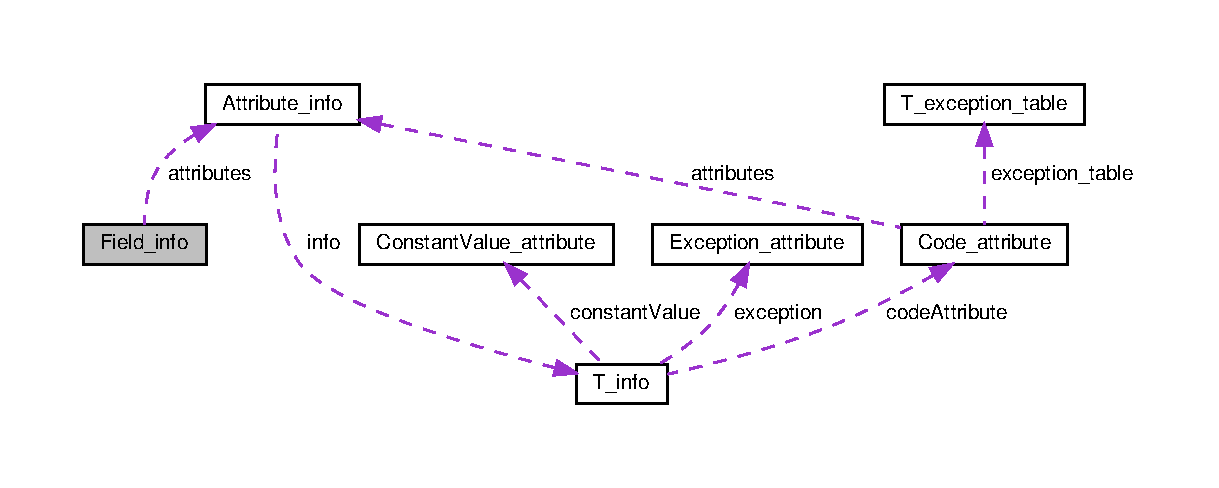
\includegraphics[width=350pt]{structField__info__coll__graph}
\end{center}
\end{figure}
\subsection*{Atributos Públicos}
\begin{DoxyCompactItemize}
\item 
unsigned char \hyperlink{structField__info_a518c6efb3e5b805d738375e3411bc7b0}{access\+Flags}
\item 
unsigned char \hyperlink{structField__info_af4d468d17e45abb44e879e9c0f0b881d}{name\+\_\+index}
\item 
unsigned char \hyperlink{structField__info_a317d816b6661095bde8c391905385f10}{descriptor\+\_\+index}
\item 
unsigned char \hyperlink{structField__info_a293084dbdbd13fce49fd95edf118db31}{attributes\+\_\+count}
\item 
\hyperlink{structAttribute__info}{Attribute\+\_\+info} $\ast$ \hyperlink{structField__info_a82d5d1b1ba57dfc6b711072777d92894}{attributes}
\end{DoxyCompactItemize}


\subsection{Descrição detalhada}
Struct responsável por armazenar os campos declarados. 

Definido na linha 18 do ficheiro Fields.\+h.



\subsection{Documentação dos dados membro}
\mbox{\Hypertarget{structField__info_a518c6efb3e5b805d738375e3411bc7b0}\label{structField__info_a518c6efb3e5b805d738375e3411bc7b0}} 
\index{Field\+\_\+info@{Field\+\_\+info}!access\+Flags@{access\+Flags}}
\index{access\+Flags@{access\+Flags}!Field\+\_\+info@{Field\+\_\+info}}
\subsubsection{\texorpdfstring{access\+Flags}{accessFlags}}
{\footnotesize\ttfamily unsigned char Field\+\_\+info\+::access\+Flags}



Definido na linha 19 do ficheiro Fields.\+h.



Referenciado por gravar\+Arquivo\+Field(), imprimir\+Field() e ler\+Field().

\mbox{\Hypertarget{structField__info_a82d5d1b1ba57dfc6b711072777d92894}\label{structField__info_a82d5d1b1ba57dfc6b711072777d92894}} 
\index{Field\+\_\+info@{Field\+\_\+info}!attributes@{attributes}}
\index{attributes@{attributes}!Field\+\_\+info@{Field\+\_\+info}}
\subsubsection{\texorpdfstring{attributes}{attributes}}
{\footnotesize\ttfamily \hyperlink{structAttribute__info}{Attribute\+\_\+info}$\ast$ Field\+\_\+info\+::attributes}



Definido na linha 23 do ficheiro Fields.\+h.



Referenciado por gravar\+Arquivo\+Field(), imprimir\+Field() e ler\+Field().

\mbox{\Hypertarget{structField__info_a293084dbdbd13fce49fd95edf118db31}\label{structField__info_a293084dbdbd13fce49fd95edf118db31}} 
\index{Field\+\_\+info@{Field\+\_\+info}!attributes\+\_\+count@{attributes\+\_\+count}}
\index{attributes\+\_\+count@{attributes\+\_\+count}!Field\+\_\+info@{Field\+\_\+info}}
\subsubsection{\texorpdfstring{attributes\+\_\+count}{attributes\_count}}
{\footnotesize\ttfamily unsigned char Field\+\_\+info\+::attributes\+\_\+count}



Definido na linha 22 do ficheiro Fields.\+h.



Referenciado por gravar\+Arquivo\+Field(), imprimir\+Field() e ler\+Field().

\mbox{\Hypertarget{structField__info_a317d816b6661095bde8c391905385f10}\label{structField__info_a317d816b6661095bde8c391905385f10}} 
\index{Field\+\_\+info@{Field\+\_\+info}!descriptor\+\_\+index@{descriptor\+\_\+index}}
\index{descriptor\+\_\+index@{descriptor\+\_\+index}!Field\+\_\+info@{Field\+\_\+info}}
\subsubsection{\texorpdfstring{descriptor\+\_\+index}{descriptor\_index}}
{\footnotesize\ttfamily unsigned char Field\+\_\+info\+::descriptor\+\_\+index}



Definido na linha 21 do ficheiro Fields.\+h.



Referenciado por gravar\+Arquivo\+Field(), imprimir\+Field(), Instance\+Class\+::\+Instance\+Class(), ler\+Field() e Static\+Class\+::\+Static\+Class().

\mbox{\Hypertarget{structField__info_af4d468d17e45abb44e879e9c0f0b881d}\label{structField__info_af4d468d17e45abb44e879e9c0f0b881d}} 
\index{Field\+\_\+info@{Field\+\_\+info}!name\+\_\+index@{name\+\_\+index}}
\index{name\+\_\+index@{name\+\_\+index}!Field\+\_\+info@{Field\+\_\+info}}
\subsubsection{\texorpdfstring{name\+\_\+index}{name\_index}}
{\footnotesize\ttfamily unsigned char Field\+\_\+info\+::name\+\_\+index}



Definido na linha 20 do ficheiro Fields.\+h.



Referenciado por gravar\+Arquivo\+Field(), imprimir\+Field(), Instance\+Class\+::\+Instance\+Class(), ler\+Field() e Static\+Class\+::\+Static\+Class().



A documentação para esta estrutura foi gerada a partir do seguinte ficheiro\+:\begin{DoxyCompactItemize}
\item 
include/\hyperlink{Fields_8h}{Fields.\+h}\end{DoxyCompactItemize}

\hypertarget{structframe__s}{}\section{Referência à estrutura frame\+\_\+s}
\label{structframe__s}\index{frame\+\_\+s@{frame\+\_\+s}}


Estrutura de armazenamento.  




{\ttfamily \#include $<$Pilha\+J\+V\+M.\+h$>$}



Diagrama de colaboração para frame\+\_\+s\+:\nopagebreak
\begin{figure}[H]
\begin{center}
\leavevmode
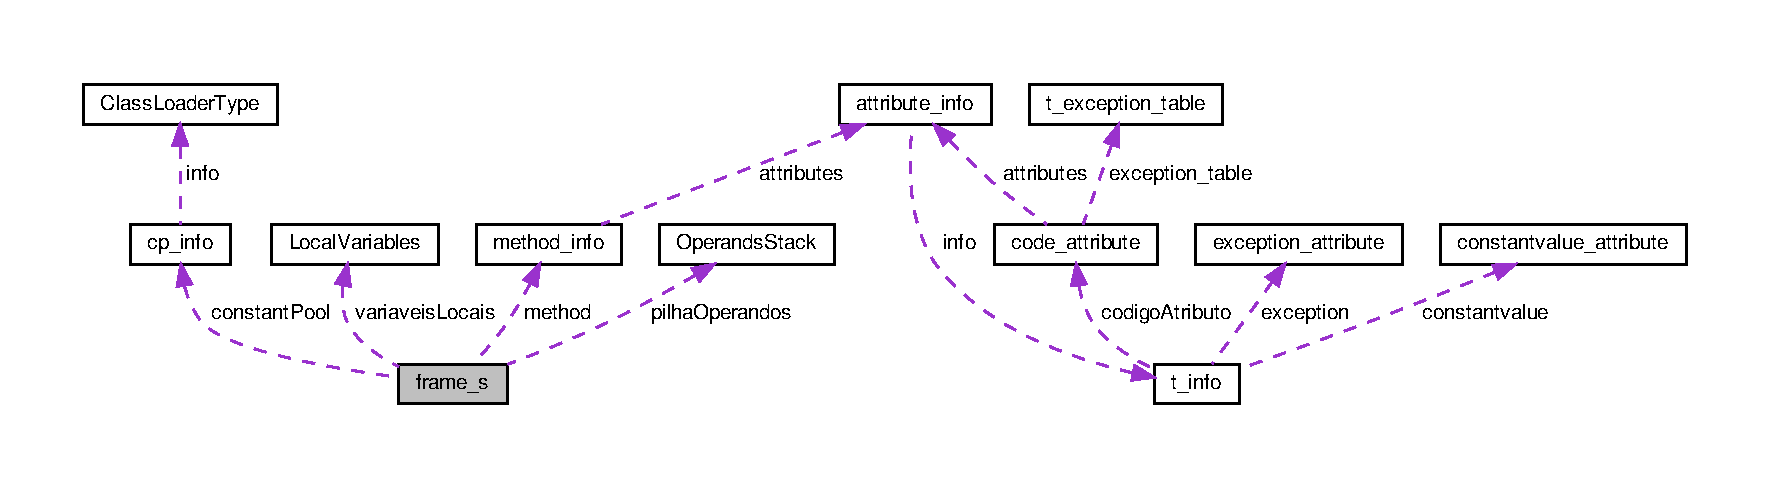
\includegraphics[width=350pt]{structframe__s__coll__graph}
\end{center}
\end{figure}
\subsection*{Atributos Públicos}
\begin{DoxyCompactItemize}
\item 
unsigned char $\ast$ \hyperlink{structframe__s_a74703c716b34b0be42af1c698ef9f621}{pc}
\item 
\hyperlink{structCp__info}{Cp\+\_\+info} $\ast$ \hyperlink{structframe__s_a87635828c425af2fef349dd22400fe99}{constant\+Pool}
\item 
\hyperlink{classOperandsStack}{Operands\+Stack} $\ast$ \hyperlink{structframe__s_ac26720ef0e7627d29c868eba6a15bfc1}{operands\+Stack}
\item 
\hyperlink{classLocalVariables}{Local\+Variables} $\ast$ \hyperlink{structframe__s_ab8c8d556e0b3a59ce604754a0e3634bb}{local\+Variables}
\item 
\hyperlink{structMethod__info}{Method\+\_\+info} \hyperlink{structframe__s_a9449132746fe7f38ff9048503b59065f}{method}
\end{DoxyCompactItemize}


\subsection{Descrição detalhada}
Estrutura de armazenamento. 

Responsável por todas as informações necessárias para a execução de um método. 

Definido na linha 25 do ficheiro Pilha\+J\+V\+M.\+h.



\subsection{Documentação dos dados membro}
\mbox{\Hypertarget{structframe__s_a87635828c425af2fef349dd22400fe99}\label{structframe__s_a87635828c425af2fef349dd22400fe99}} 
\index{frame\+\_\+s@{frame\+\_\+s}!constant\+Pool@{constant\+Pool}}
\index{constant\+Pool@{constant\+Pool}!frame\+\_\+s@{frame\+\_\+s}}
\subsubsection{\texorpdfstring{constant\+Pool}{constantPool}}
{\footnotesize\ttfamily \hyperlink{structCp__info}{Cp\+\_\+info}$\ast$ frame\+\_\+s\+::constant\+Pool}



Definido na linha 27 do ficheiro Pilha\+J\+V\+M.\+h.



Referenciado por Pilha\+J\+V\+M\+::adicionar\+Frame(), Operations\+::func\+\_\+new(), Operations\+::getfield(), Operations\+::getstatic(), Operations\+::invokeinterface(), Operations\+::invokespecial(), Operations\+::invokestatic(), Operations\+::invokevirtual(), Operations\+::ldc(), Operations\+::ldc2\+\_\+w(), Operations\+::ldc\+\_\+w(), Operations\+::multianewarray(), Pilha\+J\+V\+M\+::\+Pilha\+J\+V\+M(), Operations\+::putfield() e Operations\+::putstatic().

\mbox{\Hypertarget{structframe__s_ab8c8d556e0b3a59ce604754a0e3634bb}\label{structframe__s_ab8c8d556e0b3a59ce604754a0e3634bb}} 
\index{frame\+\_\+s@{frame\+\_\+s}!local\+Variables@{local\+Variables}}
\index{local\+Variables@{local\+Variables}!frame\+\_\+s@{frame\+\_\+s}}
\subsubsection{\texorpdfstring{local\+Variables}{localVariables}}
{\footnotesize\ttfamily \hyperlink{classLocalVariables}{Local\+Variables}$\ast$ frame\+\_\+s\+::local\+Variables}



Definido na linha 29 do ficheiro Pilha\+J\+V\+M.\+h.



Referenciado por Pilha\+J\+V\+M\+::adicionar\+Frame(), Operations\+::aload(), Operations\+::aload\+\_\+n(), Operations\+::astore(), Operations\+::astore\+\_\+0(), Operations\+::astore\+\_\+1(), Operations\+::astore\+\_\+2(), Operations\+::astore\+\_\+3(), Operations\+::dload(), Operations\+::dload\+\_\+n(), Operations\+::dstore(), Operations\+::dstore\+\_\+0(), Operations\+::dstore\+\_\+1(), Operations\+::dstore\+\_\+2(), Operations\+::dstore\+\_\+3(), Operations\+::fload(), Operations\+::fload\+\_\+n(), Operations\+::fstore(), Operations\+::fstore\+\_\+0(), Operations\+::fstore\+\_\+1(), Operations\+::fstore\+\_\+2(), Operations\+::fstore\+\_\+3(), Operations\+::funcret(), Operations\+::iinc(), Operations\+::iload(), Operations\+::iload\+\_\+0(), Operations\+::iload\+\_\+1(), Operations\+::iload\+\_\+2(), Operations\+::iload\+\_\+3(), Operations\+::istore(), Operations\+::istore\+\_\+0(), Operations\+::istore\+\_\+1(), Operations\+::istore\+\_\+2(), Operations\+::istore\+\_\+3(), Operations\+::lload(), Operations\+::lload\+\_\+n(), Operations\+::lstore(), Operations\+::lstore\+\_\+0(), Operations\+::lstore\+\_\+1(), Operations\+::lstore\+\_\+2(), Operations\+::lstore\+\_\+3() e Pilha\+J\+V\+M\+::\+Pilha\+J\+V\+M().

\mbox{\Hypertarget{structframe__s_a9449132746fe7f38ff9048503b59065f}\label{structframe__s_a9449132746fe7f38ff9048503b59065f}} 
\index{frame\+\_\+s@{frame\+\_\+s}!method@{method}}
\index{method@{method}!frame\+\_\+s@{frame\+\_\+s}}
\subsubsection{\texorpdfstring{method}{method}}
{\footnotesize\ttfamily \hyperlink{structMethod__info}{Method\+\_\+info} frame\+\_\+s\+::method}



Definido na linha 30 do ficheiro Pilha\+J\+V\+M.\+h.



Referenciado por Pilha\+J\+V\+M\+::adicionar\+Frame(), Pilha\+J\+V\+M\+::inicializar\+P\+C(), Operations\+::lookupswitch(), Pilha\+J\+V\+M\+::\+Pilha\+J\+V\+M(), Operations\+::putfield() e Operations\+::tableswitch().

\mbox{\Hypertarget{structframe__s_ac26720ef0e7627d29c868eba6a15bfc1}\label{structframe__s_ac26720ef0e7627d29c868eba6a15bfc1}} 
\index{frame\+\_\+s@{frame\+\_\+s}!operands\+Stack@{operands\+Stack}}
\index{operands\+Stack@{operands\+Stack}!frame\+\_\+s@{frame\+\_\+s}}
\subsubsection{\texorpdfstring{operands\+Stack}{operandsStack}}
{\footnotesize\ttfamily \hyperlink{classOperandsStack}{Operands\+Stack}$\ast$ frame\+\_\+s\+::operands\+Stack}



Definido na linha 28 do ficheiro Pilha\+J\+V\+M.\+h.



Referenciado por Operations\+::aaload(), Operations\+::aastore(), Operations\+::aconst\+\_\+null(), Pilha\+J\+V\+M\+::adicionar\+Frame(), Operations\+::aload(), Operations\+::aload\+\_\+n(), Operations\+::anewarray(), Operations\+::areturn(), Operations\+::arraylength(), Operations\+::astore(), Operations\+::astore\+\_\+0(), Operations\+::astore\+\_\+1(), Operations\+::astore\+\_\+2(), Operations\+::astore\+\_\+3(), Operations\+::athrow(), Operations\+::baload(), Operations\+::bastore(), Operations\+::bipush(), Operations\+::caload(), Operations\+::castore(), Operations\+::d2f(), Operations\+::d2i(), Operations\+::d2l(), Operations\+::dadd(), Operations\+::daload(), Operations\+::dastore(), Operations\+::dcmpg(), Operations\+::dcmpl(), Operations\+::dconst\+\_\+0(), Operations\+::dconst\+\_\+1(), Operations\+::ddiv(), Operations\+::dload(), Operations\+::dload\+\_\+n(), Operations\+::dmul(), Operations\+::dneg(), Operations\+::drem(), Operations\+::dreturn(), Operations\+::dstore(), Operations\+::dstore\+\_\+0(), Operations\+::dstore\+\_\+1(), Operations\+::dstore\+\_\+2(), Operations\+::dstore\+\_\+3(), Operations\+::dsub(), Operations\+::dup(), Operations\+::dup2(), Operations\+::dup2\+\_\+x1(), Operations\+::dup2\+\_\+x2(), Operations\+::dup\+\_\+x1(), Operations\+::dup\+\_\+x2(), Operations\+::f2d(), Operations\+::f2i(), Operations\+::f2l(), Operations\+::fadd(), Operations\+::faload(), Operations\+::fastore(), Operations\+::fcmpg(), Operations\+::fcmpl(), Operations\+::fconst\+\_\+0(), Operations\+::fconst\+\_\+1(), Operations\+::fconst\+\_\+2(), Operations\+::fdiv(), Operations\+::fload(), Operations\+::fload\+\_\+n(), Operations\+::fmul(), Operations\+::fneg(), Operations\+::frem(), Operations\+::freturn(), Operations\+::fstore(), Operations\+::fstore\+\_\+0(), Operations\+::fstore\+\_\+1(), Operations\+::fstore\+\_\+2(), Operations\+::fstore\+\_\+3(), Operations\+::fsub(), Operations\+::func\+\_\+new(), Operations\+::func\+\_\+return(), Operations\+::getfield(), Operations\+::getstatic(), Operations\+::i2b(), Operations\+::i2c(), Operations\+::i2d(), Operations\+::i2f(), Operations\+::i2l(), Operations\+::i2s(), Operations\+::iadd(), Operations\+::iaload(), Operations\+::iand(), Operations\+::iastore(), Operations\+::iconst\+\_\+0(), Operations\+::iconst\+\_\+1(), Operations\+::iconst\+\_\+2(), Operations\+::iconst\+\_\+3(), Operations\+::iconst\+\_\+4(), Operations\+::iconst\+\_\+5(), Operations\+::iconst\+\_\+m1(), Operations\+::idiv(), Operations\+::if\+\_\+acmpeq(), Operations\+::if\+\_\+acmpne(), Operations\+::if\+\_\+icmpeq(), Operations\+::if\+\_\+icmpge(), Operations\+::if\+\_\+icmpgt(), Operations\+::if\+\_\+icmple(), Operations\+::if\+\_\+icmplt(), Operations\+::if\+\_\+icmpne(), Operations\+::ifeq(), Operations\+::ifge(), Operations\+::ifgt(), Operations\+::ifle(), Operations\+::iflt(), Operations\+::ifne(), Operations\+::ifnonnull(), Operations\+::ifnull(), Operations\+::iload(), Operations\+::iload\+\_\+0(), Operations\+::iload\+\_\+1(), Operations\+::iload\+\_\+2(), Operations\+::iload\+\_\+3(), Operations\+::imul(), Operations\+::ineg(), Operations\+::invokeinterface(), Operations\+::invokespecial(), Operations\+::invokestatic(), Operations\+::invokevirtual(), Operations\+::ior(), Operations\+::irem(), Operations\+::ireturn(), Operations\+::ishl(), Operations\+::ishr(), Operations\+::istore(), Operations\+::istore\+\_\+0(), Operations\+::istore\+\_\+1(), Operations\+::istore\+\_\+2(), Operations\+::istore\+\_\+3(), Operations\+::isub(), Operations\+::iushr(), Operations\+::ixor(), Operations\+::jsr(), Operations\+::jsr\+\_\+w(), Operations\+::l2d(), Operations\+::l2f(), Operations\+::l2i(), Operations\+::ladd(), Operations\+::laload(), Operations\+::land(), Operations\+::lastore(), Operations\+::lcmp(), Operations\+::lconst\+\_\+0(), Operations\+::lconst\+\_\+1(), Operations\+::ldc(), Operations\+::ldc2\+\_\+w(), Operations\+::ldc\+\_\+w(), Operations\+::ldiv(), Operations\+::lload(), Operations\+::lload\+\_\+n(), Operations\+::lmul(), Operations\+::lneg(), Operations\+::lookupswitch(), Operations\+::lor(), Operations\+::lrem(), Operations\+::lreturn(), Operations\+::lshl(), Operations\+::lshr(), Operations\+::lstore(), Operations\+::lstore\+\_\+0(), Operations\+::lstore\+\_\+1(), Operations\+::lstore\+\_\+2(), Operations\+::lstore\+\_\+3(), Operations\+::lsub(), Operations\+::lushr(), Operations\+::lxor(), Operations\+::multianewarray(), Operations\+::newarray(), Pilha\+J\+V\+M\+::\+Pilha\+J\+V\+M(), Operations\+::pop(), Operations\+::pop2(), Operations\+::putfield(), Operations\+::putstatic(), Operations\+::saload(), Operations\+::sastore(), Operations\+::sipush(), Operations\+::swap() e Operations\+::tableswitch().

\mbox{\Hypertarget{structframe__s_a74703c716b34b0be42af1c698ef9f621}\label{structframe__s_a74703c716b34b0be42af1c698ef9f621}} 
\index{frame\+\_\+s@{frame\+\_\+s}!pc@{pc}}
\index{pc@{pc}!frame\+\_\+s@{frame\+\_\+s}}
\subsubsection{\texorpdfstring{pc}{pc}}
{\footnotesize\ttfamily unsigned char$\ast$ frame\+\_\+s\+::pc}



Definido na linha 26 do ficheiro Pilha\+J\+V\+M.\+h.



Referenciado por Operations\+::aload(), Operations\+::anewarray(), Operations\+::astore(), Operations\+::bipush(), Operations\+::dload(), Operations\+::dstore(), Operations\+::fload(), Operations\+::fstore(), Operations\+::func\+\_\+new(), Operations\+::funcgoto(), Operations\+::funcret(), Operations\+::getfield(), Operations\+::getstatic(), Operations\+::goto\+\_\+w(), Operations\+::if\+\_\+acmpeq(), Operations\+::if\+\_\+acmpne(), Operations\+::if\+\_\+icmpeq(), Operations\+::if\+\_\+icmpge(), Operations\+::if\+\_\+icmpgt(), Operations\+::if\+\_\+icmple(), Operations\+::if\+\_\+icmplt(), Operations\+::if\+\_\+icmpne(), Operations\+::ifeq(), Operations\+::ifge(), Operations\+::ifgt(), Operations\+::ifle(), Operations\+::iflt(), Operations\+::ifne(), Operations\+::ifnonnull(), Operations\+::ifnull(), Operations\+::iinc(), Operations\+::iload(), Pilha\+J\+V\+M\+::inicializar\+P\+C(), Operations\+::invokeinterface(), Operations\+::invokespecial(), Operations\+::invokestatic(), Operations\+::invokevirtual(), Operations\+::istore(), Operations\+::jsr(), Operations\+::jsr\+\_\+w(), Operations\+::ldc(), Operations\+::ldc2\+\_\+w(), Operations\+::ldc\+\_\+w(), Operations\+::lload(), Operations\+::lookupswitch(), Operations\+::lstore(), Operations\+::multianewarray(), Operations\+::newarray(), Operations\+::putfield(), Operations\+::putstatic(), Operations\+::sipush(), Operations\+::tableswitch() e Operations\+::wide().



A documentação para esta estrutura foi gerada a partir do seguinte ficheiro\+:\begin{DoxyCompactItemize}
\item 
include/\hyperlink{PilhaJVM_8h}{Pilha\+J\+V\+M.\+h}\end{DoxyCompactItemize}

\hypertarget{classHeap}{}\section{Referência à classe Heap}
\label{classHeap}\index{Heap@{Heap}}


Gerencia as operações do heap.  




{\ttfamily \#include $<$Heap.\+h$>$}

\subsection*{Membros públicos}
\begin{DoxyCompactItemize}
\item 
\hyperlink{classHeap_a734051272cbd0945d3916a1a89707ba2}{$\sim$\+Heap} ()
\begin{DoxyCompactList}\small\item\em Destrutor padrão. \end{DoxyCompactList}\item 
void \hyperlink{classHeap_aa2a5f92b36abe24c83853feca936548e}{add\+Object} (\hyperlink{classObject}{Object} $\ast$object)
\begin{DoxyCompactList}\small\item\em Adiciona um objeto à heap. \end{DoxyCompactList}\end{DoxyCompactItemize}
\subsection*{Membros públicos estáticos}
\begin{DoxyCompactItemize}
\item 
static \hyperlink{classHeap}{Heap} \& \hyperlink{classHeap_ac030780aeff8a27e33ed5f5eb576dfda}{get\+Instance} ()
\begin{DoxyCompactList}\small\item\em Obter a única instância da \hyperlink{classHeap}{Heap}. \end{DoxyCompactList}\end{DoxyCompactItemize}
\subsection*{Membros privados}
\begin{DoxyCompactItemize}
\item 
\hyperlink{classHeap_a6595efd3562a6334d2f5471c2b3b7cb4}{Heap} ()
\item 
\hyperlink{classHeap_aac9a075f0c23c3923fabbf2093386089}{Heap} (\hyperlink{classHeap}{Heap} const \&)
\item 
void \hyperlink{classHeap_a2923f4b4b05267583815e185f2e28b7d}{operator=} (\hyperlink{classHeap}{Heap} const \&)
\end{DoxyCompactItemize}
\subsection*{Atributos Privados}
\begin{DoxyCompactItemize}
\item 
vector$<$ \hyperlink{classObject}{Object} $\ast$ $>$ \hyperlink{classHeap_a55b6cf9504fbe890a49e667c80dae717}{\+\_\+object\+Vector}
\end{DoxyCompactItemize}


\subsection{Descrição detalhada}
Gerencia as operações do heap. 

Essa classe é um singleton, ou seja, somente existe no máximo 1 instância dela para cada instância da J\+VM. 

Definido na linha 16 do ficheiro Heap.\+h.



\subsection{Documentação dos Construtores \& Destrutor}
\mbox{\Hypertarget{classHeap_a734051272cbd0945d3916a1a89707ba2}\label{classHeap_a734051272cbd0945d3916a1a89707ba2}} 
\index{Heap@{Heap}!````~Heap@{$\sim$\+Heap}}
\index{````~Heap@{$\sim$\+Heap}!Heap@{Heap}}
\subsubsection{\texorpdfstring{$\sim$\+Heap()}{~Heap()}}
{\footnotesize\ttfamily Heap\+::$\sim$\+Heap (\begin{DoxyParamCaption}{ }\end{DoxyParamCaption})}



Destrutor padrão. 



Definido na linha 11 do ficheiro Heap.\+cpp.

\mbox{\Hypertarget{classHeap_a6595efd3562a6334d2f5471c2b3b7cb4}\label{classHeap_a6595efd3562a6334d2f5471c2b3b7cb4}} 
\index{Heap@{Heap}!Heap@{Heap}}
\index{Heap@{Heap}!Heap@{Heap}}
\subsubsection{\texorpdfstring{Heap()}{Heap()}\hspace{0.1cm}{\footnotesize\ttfamily [1/2]}}
{\footnotesize\ttfamily Heap\+::\+Heap (\begin{DoxyParamCaption}{ }\end{DoxyParamCaption})\hspace{0.3cm}{\ttfamily [private]}}

Construtor padrão. 

Definido na linha 7 do ficheiro Heap.\+cpp.

\mbox{\Hypertarget{classHeap_aac9a075f0c23c3923fabbf2093386089}\label{classHeap_aac9a075f0c23c3923fabbf2093386089}} 
\index{Heap@{Heap}!Heap@{Heap}}
\index{Heap@{Heap}!Heap@{Heap}}
\subsubsection{\texorpdfstring{Heap()}{Heap()}\hspace{0.1cm}{\footnotesize\ttfamily [2/2]}}
{\footnotesize\ttfamily Heap\+::\+Heap (\begin{DoxyParamCaption}\item[{\hyperlink{classHeap}{Heap} const \&}]{ }\end{DoxyParamCaption})\hspace{0.3cm}{\ttfamily [private]}}



\subsection{Documentação dos métodos}
\mbox{\Hypertarget{classHeap_aa2a5f92b36abe24c83853feca936548e}\label{classHeap_aa2a5f92b36abe24c83853feca936548e}} 
\index{Heap@{Heap}!add\+Object@{add\+Object}}
\index{add\+Object@{add\+Object}!Heap@{Heap}}
\subsubsection{\texorpdfstring{add\+Object()}{addObject()}}
{\footnotesize\ttfamily void Heap\+::add\+Object (\begin{DoxyParamCaption}\item[{\hyperlink{classObject}{Object} $\ast$}]{object }\end{DoxyParamCaption})}



Adiciona um objeto à heap. 



Definido na linha 15 do ficheiro Heap.\+cpp.



Referenciado por Instance\+Class\+::\+Instance\+Class().

\mbox{\Hypertarget{classHeap_ac030780aeff8a27e33ed5f5eb576dfda}\label{classHeap_ac030780aeff8a27e33ed5f5eb576dfda}} 
\index{Heap@{Heap}!get\+Instance@{get\+Instance}}
\index{get\+Instance@{get\+Instance}!Heap@{Heap}}
\subsubsection{\texorpdfstring{get\+Instance()}{getInstance()}}
{\footnotesize\ttfamily static \hyperlink{classHeap}{Heap}\& Heap\+::get\+Instance (\begin{DoxyParamCaption}{ }\end{DoxyParamCaption})\hspace{0.3cm}{\ttfamily [inline]}, {\ttfamily [static]}}



Obter a única instância da \hyperlink{classHeap}{Heap}. 

\begin{DoxyReturn}{Retorna}
A instância da \hyperlink{classHeap}{Heap}. 
\end{DoxyReturn}


Definido na linha 22 do ficheiro Heap.\+h.



Referenciado por Instance\+Class\+::\+Instance\+Class().

\mbox{\Hypertarget{classHeap_a2923f4b4b05267583815e185f2e28b7d}\label{classHeap_a2923f4b4b05267583815e185f2e28b7d}} 
\index{Heap@{Heap}!operator=@{operator=}}
\index{operator=@{operator=}!Heap@{Heap}}
\subsubsection{\texorpdfstring{operator=()}{operator=()}}
{\footnotesize\ttfamily void Heap\+::operator= (\begin{DoxyParamCaption}\item[{\hyperlink{classHeap}{Heap} const \&}]{ }\end{DoxyParamCaption})\hspace{0.3cm}{\ttfamily [private]}}



\subsection{Documentação dos dados membro}
\mbox{\Hypertarget{classHeap_a55b6cf9504fbe890a49e667c80dae717}\label{classHeap_a55b6cf9504fbe890a49e667c80dae717}} 
\index{Heap@{Heap}!\+\_\+object\+Vector@{\+\_\+object\+Vector}}
\index{\+\_\+object\+Vector@{\+\_\+object\+Vector}!Heap@{Heap}}
\subsubsection{\texorpdfstring{\+\_\+object\+Vector}{\_objectVector}}
{\footnotesize\ttfamily vector$<$\hyperlink{classObject}{Object}$\ast$$>$ Heap\+::\+\_\+object\+Vector\hspace{0.3cm}{\ttfamily [private]}}

Vetor interno que armazena todos os objetos. 

Definido na linha 49 do ficheiro Heap.\+h.



A documentação para esta classe foi gerada a partir dos seguintes ficheiros\+:\begin{DoxyCompactItemize}
\item 
include/\hyperlink{Heap_8h}{Heap.\+h}\item 
src/\hyperlink{Heap_8cpp}{Heap.\+cpp}\end{DoxyCompactItemize}

\hypertarget{classInstance}{}\section{Referência à classe Instance}
\label{classInstance}\index{Instance@{Instance}}


Class instantiation.  




{\ttfamily \#include $<$Instance\+Class.\+h$>$}



\subsection{Descrição detalhada}
Class instantiation. 

Lida com operações que lidam com uma instância da classe 

A documentação para esta classe foi gerada a partir do seguinte ficheiro\+:\begin{DoxyCompactItemize}
\item 
include/\hyperlink{InstanceClass_8h}{Instance\+Class.\+h}\end{DoxyCompactItemize}

\hypertarget{classInstanceClass}{}\section{Referência à classe Instance\+Class}
\label{classInstanceClass}\index{Instance\+Class@{Instance\+Class}}


Lida com operações que lidam com uma instância da classe.  




{\ttfamily \#include $<$Instance\+Class.\+h$>$}



Diagrama de heranças da classe Instance\+Class\nopagebreak
\begin{figure}[H]
\begin{center}
\leavevmode
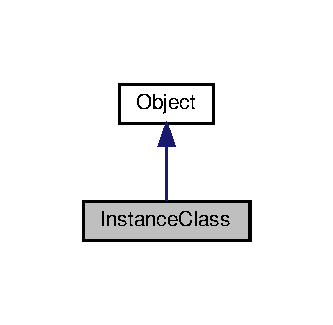
\includegraphics[width=160pt]{classInstanceClass__inherit__graph}
\end{center}
\end{figure}


Diagrama de colaboração para Instance\+Class\+:\nopagebreak
\begin{figure}[H]
\begin{center}
\leavevmode
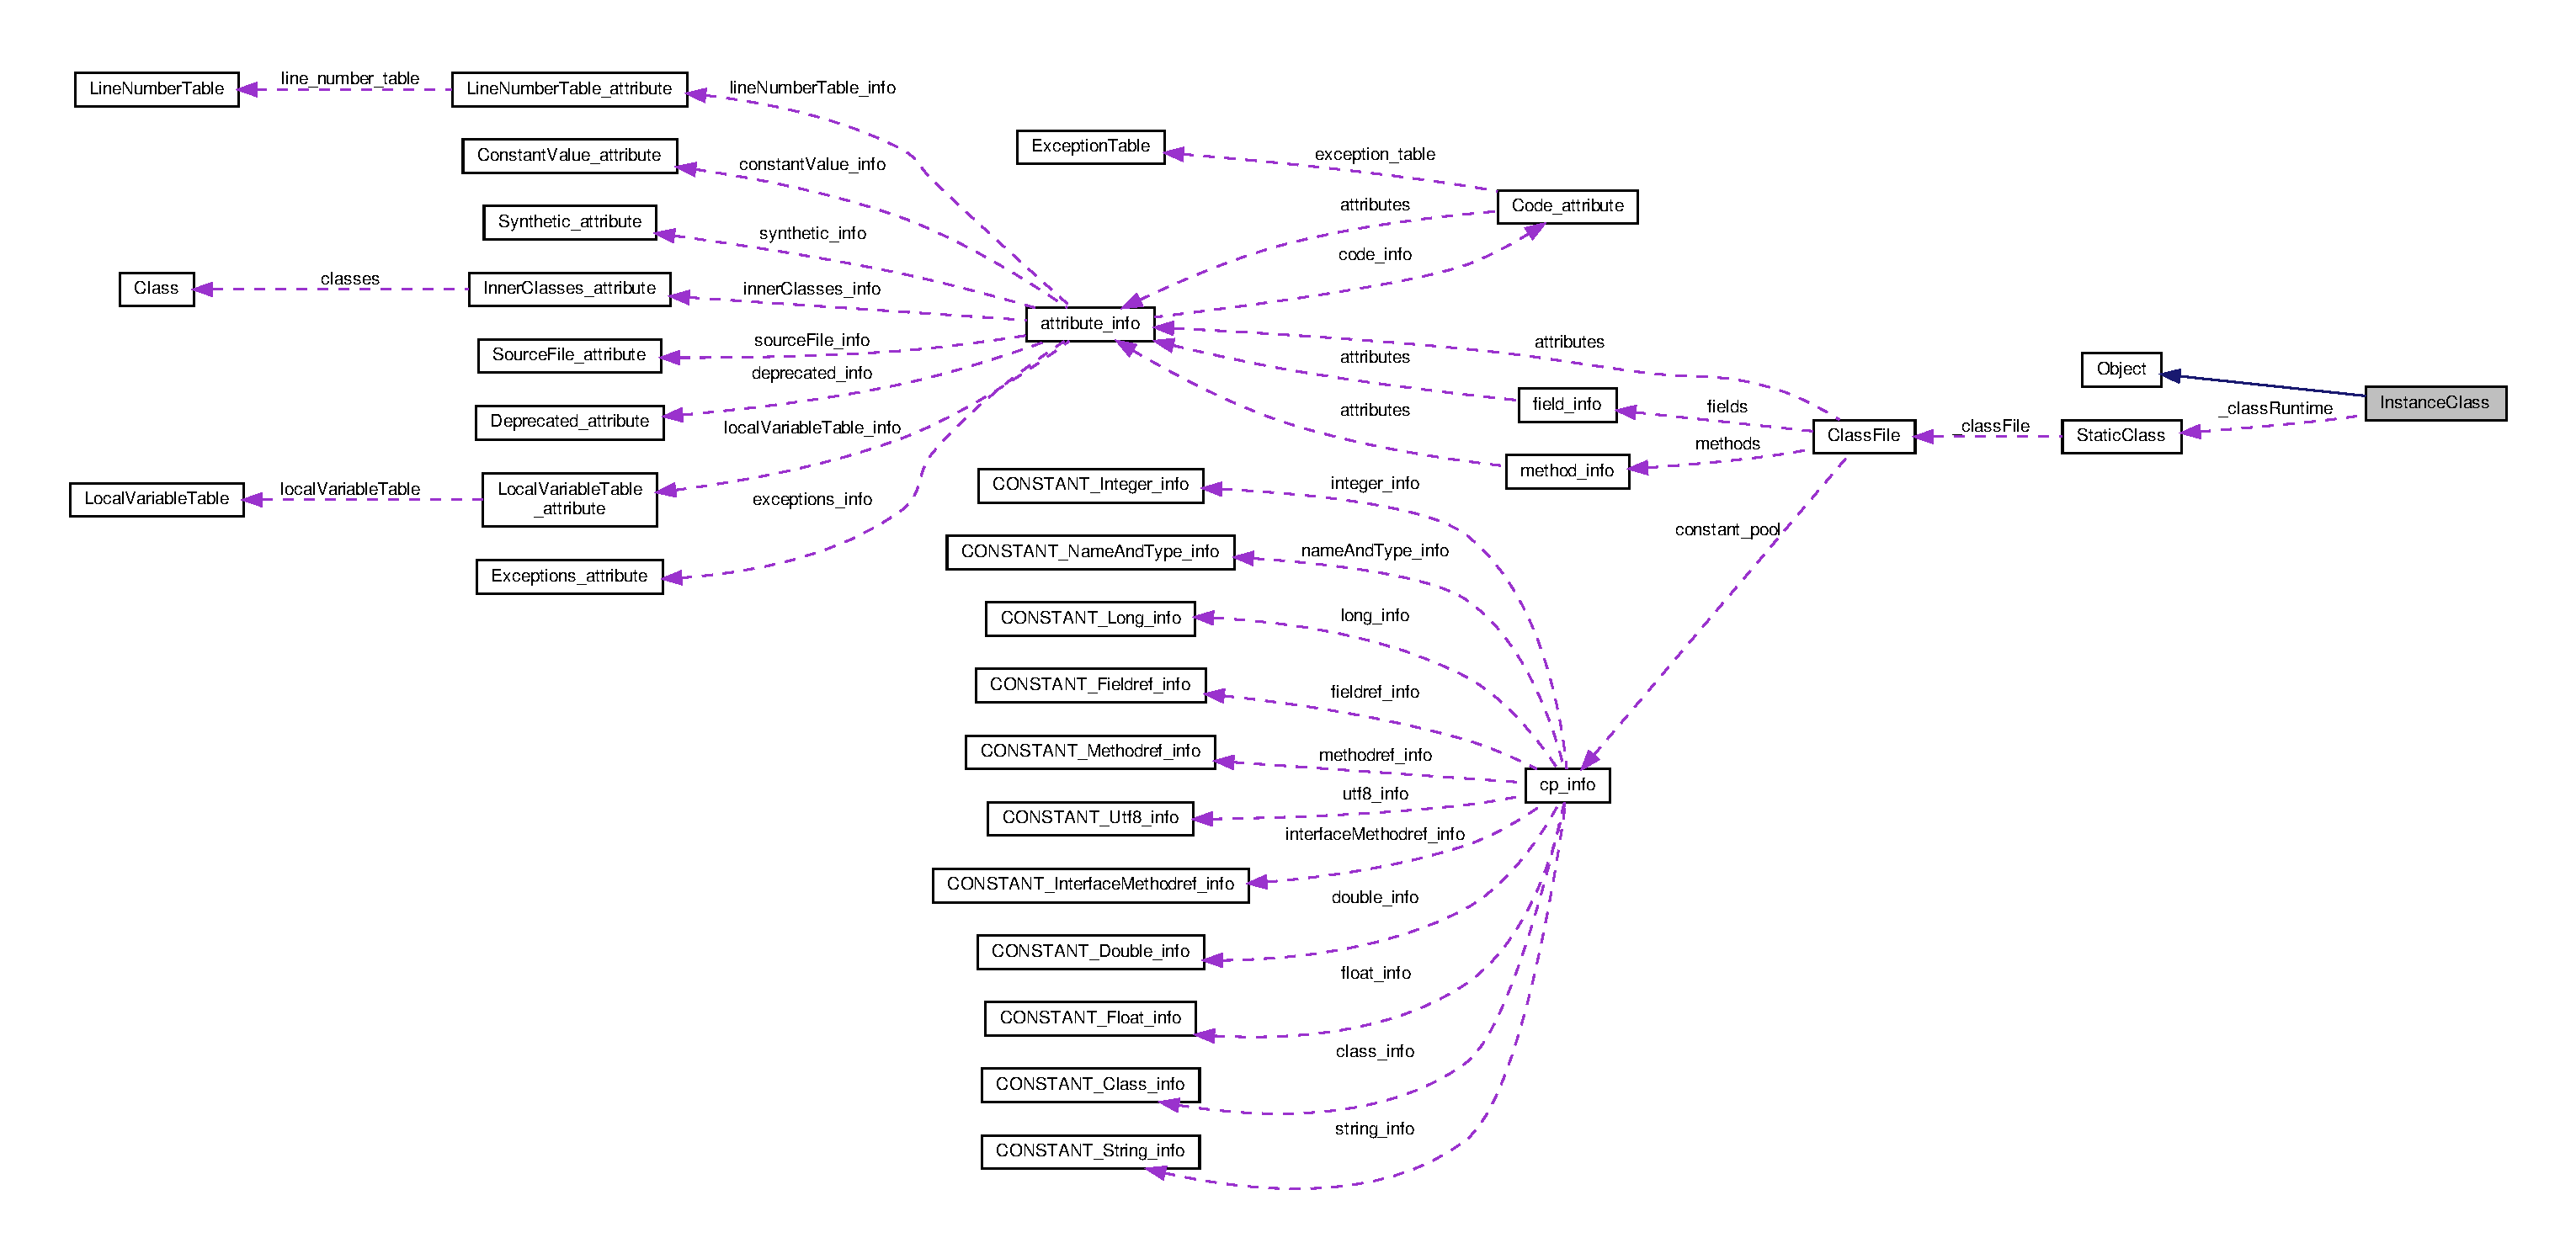
\includegraphics[width=350pt]{classInstanceClass__coll__graph}
\end{center}
\end{figure}
\subsection*{Membros públicos}
\begin{DoxyCompactItemize}
\item 
\hyperlink{classInstanceClass_a86ab031eb0f0240b0a54423003000322}{Instance\+Class} (\hyperlink{classStaticClass}{Static\+Class} $\ast$class\+Runtime)
\begin{DoxyCompactList}\small\item\em Construtor padrão. \end{DoxyCompactList}\item 
\hyperlink{classInstanceClass_a441cc692dedc481373b7e670fab72556}{$\sim$\+Instance\+Class} ()
\begin{DoxyCompactList}\small\item\em Destrutor padrão. \end{DoxyCompactList}\item 
\hyperlink{BasicTypes_8h_a842c5e2e69277690b064bf363c017980}{Object\+Type} \hyperlink{classInstanceClass_ae8570307f49cb95cc01fb8d6bda23763}{object\+Type} ()
\begin{DoxyCompactList}\small\item\em Método utilizado para declaração do tipo de objeto. \end{DoxyCompactList}\item 
\hyperlink{classStaticClass}{Static\+Class} $\ast$ \hyperlink{classInstanceClass_adf2af3015bb8f777a3181d85aa279de8}{get\+Class\+Runtime} ()
\begin{DoxyCompactList}\small\item\em Obtém a classe correspondente ao objeto. \end{DoxyCompactList}\item 
void \hyperlink{classInstanceClass_af445c2e244c91b6cce4bb2c2798a720c}{put\+Value\+Into\+Field} (\hyperlink{structValue}{Value} value, string field\+Name)
\begin{DoxyCompactList}\small\item\em Adiciona um valor no field de índice informado. \end{DoxyCompactList}\item 
\hyperlink{structValue}{Value} \hyperlink{classInstanceClass_aee974c71919d470ea2e9aa75cf741a39}{get\+Value\+From\+Field} (string field\+Name)
\begin{DoxyCompactList}\small\item\em Obtém o valor contido em um field informado. \end{DoxyCompactList}\item 
bool \hyperlink{classInstanceClass_a284c7d0a062623c614a2f9440340070f}{field\+Exists} (string field\+Name)
\begin{DoxyCompactList}\small\item\em Verifica se existe um field com o nome dado. \end{DoxyCompactList}\end{DoxyCompactItemize}
\subsection*{Atributos Privados}
\begin{DoxyCompactItemize}
\item 
\hyperlink{classStaticClass}{Static\+Class} $\ast$ \hyperlink{classInstanceClass_aa8ed961b694f26f470dc2399532d3538}{\+\_\+class\+Runtime}
\item 
map$<$ string, \hyperlink{structValue}{Value} $>$ \hyperlink{classInstanceClass_a603a0866f5113d16ff8f80b5d6bf152b}{\+\_\+fields}
\end{DoxyCompactItemize}


\subsection{Descrição detalhada}
Lida com operações que lidam com uma instância da classe. 

Definido na linha 18 do ficheiro Instance\+Class.\+h.



\subsection{Documentação dos Construtores \& Destrutor}
\mbox{\Hypertarget{classInstanceClass_a86ab031eb0f0240b0a54423003000322}\label{classInstanceClass_a86ab031eb0f0240b0a54423003000322}} 
\index{Instance\+Class@{Instance\+Class}!Instance\+Class@{Instance\+Class}}
\index{Instance\+Class@{Instance\+Class}!Instance\+Class@{Instance\+Class}}
\subsubsection{\texorpdfstring{Instance\+Class()}{InstanceClass()}}
{\footnotesize\ttfamily Instance\+Class\+::\+Instance\+Class (\begin{DoxyParamCaption}\item[{\hyperlink{classStaticClass}{Static\+Class} $\ast$}]{class\+Runtime }\end{DoxyParamCaption})}



Construtor padrão. 


\begin{DoxyParams}{Parâmetros}
{\em class\+Runtime} & A classe correspondente ao objeto. \\
\hline
\end{DoxyParams}


Definido na linha 9 do ficheiro Instance\+Class.\+cpp.



Referências Class\+File\+::access\+\_\+flags, field\+\_\+info\+::access\+\_\+flags, Heap\+::add\+Object(), B\+O\+O\+L\+E\+AN, B\+Y\+TE, Value\+::byte\+Value, C\+H\+AR, Value\+::char\+Value, Class\+File\+::constant\+\_\+pool, Value\+::data, field\+\_\+info\+::descriptor\+\_\+index, D\+O\+U\+B\+LE, Value\+::double\+Value, Class\+File\+::fields, Class\+File\+::fields\+\_\+count, F\+L\+O\+AT, Value\+::float\+Value, Static\+Class\+::get\+Class\+File(), get\+Formatted\+Constant(), Heap\+::get\+Instance(), I\+NT, Value\+::int\+Value, L\+O\+NG, Value\+::long\+Value, field\+\_\+info\+::name\+\_\+index, Value\+::object, put\+Value\+Into\+Field(), R\+E\+F\+E\+R\+E\+N\+CE, S\+H\+O\+RT, Value\+::short\+Value e Value\+::type.

Grafo de chamadas desta função\+:\nopagebreak
\begin{figure}[H]
\begin{center}
\leavevmode
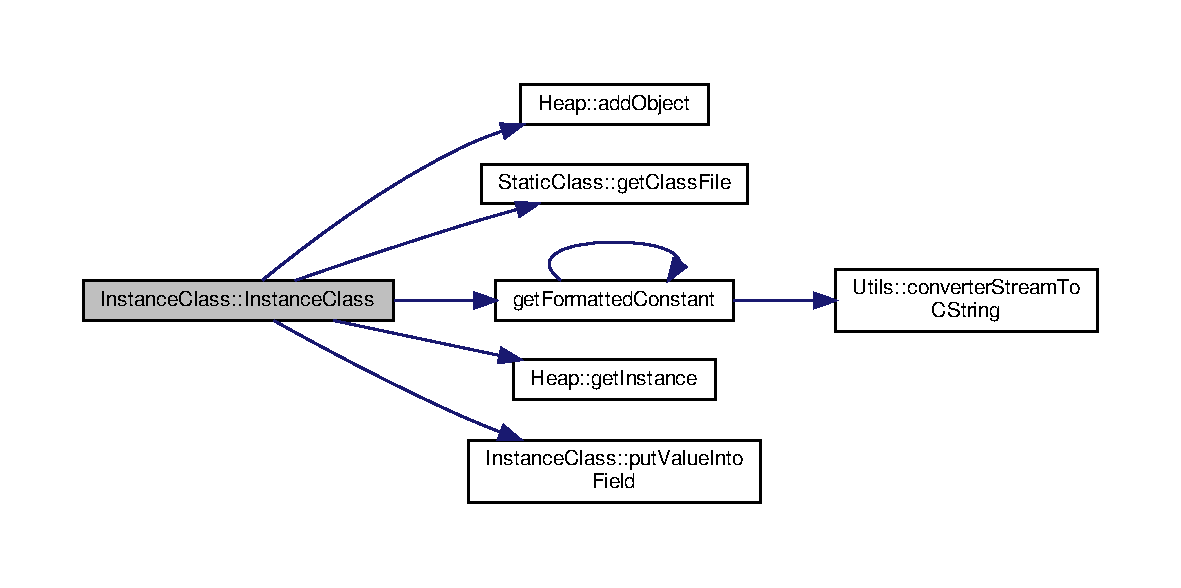
\includegraphics[width=350pt]{classInstanceClass_a86ab031eb0f0240b0a54423003000322_cgraph}
\end{center}
\end{figure}
\mbox{\Hypertarget{classInstanceClass_a441cc692dedc481373b7e670fab72556}\label{classInstanceClass_a441cc692dedc481373b7e670fab72556}} 
\index{Instance\+Class@{Instance\+Class}!````~Instance\+Class@{$\sim$\+Instance\+Class}}
\index{````~Instance\+Class@{$\sim$\+Instance\+Class}!Instance\+Class@{Instance\+Class}}
\subsubsection{\texorpdfstring{$\sim$\+Instance\+Class()}{~InstanceClass()}}
{\footnotesize\ttfamily Instance\+Class\+::$\sim$\+Instance\+Class (\begin{DoxyParamCaption}{ }\end{DoxyParamCaption})}



Destrutor padrão. 



Definido na linha 79 do ficheiro Instance\+Class.\+cpp.



\subsection{Documentação dos métodos}
\mbox{\Hypertarget{classInstanceClass_a284c7d0a062623c614a2f9440340070f}\label{classInstanceClass_a284c7d0a062623c614a2f9440340070f}} 
\index{Instance\+Class@{Instance\+Class}!field\+Exists@{field\+Exists}}
\index{field\+Exists@{field\+Exists}!Instance\+Class@{Instance\+Class}}
\subsubsection{\texorpdfstring{field\+Exists()}{fieldExists()}}
{\footnotesize\ttfamily bool Instance\+Class\+::field\+Exists (\begin{DoxyParamCaption}\item[{string}]{field\+Name }\end{DoxyParamCaption})}



Verifica se existe um field com o nome dado. 


\begin{DoxyParams}{Parâmetros}
{\em field\+Name} & O nome do field. \\
\hline
\end{DoxyParams}
\begin{DoxyReturn}{Retorna}
Retorna {\ttfamily true} caso o field existir, e {\ttfamily false} caso contrário. 
\end{DoxyReturn}


Definido na linha 104 do ficheiro Instance\+Class.\+cpp.



Referências \+\_\+fields.

\mbox{\Hypertarget{classInstanceClass_adf2af3015bb8f777a3181d85aa279de8}\label{classInstanceClass_adf2af3015bb8f777a3181d85aa279de8}} 
\index{Instance\+Class@{Instance\+Class}!get\+Class\+Runtime@{get\+Class\+Runtime}}
\index{get\+Class\+Runtime@{get\+Class\+Runtime}!Instance\+Class@{Instance\+Class}}
\subsubsection{\texorpdfstring{get\+Class\+Runtime()}{getClassRuntime()}}
{\footnotesize\ttfamily \hyperlink{classStaticClass}{Static\+Class} $\ast$ Instance\+Class\+::get\+Class\+Runtime (\begin{DoxyParamCaption}{ }\end{DoxyParamCaption})}



Obtém a classe correspondente ao objeto. 

\begin{DoxyReturn}{Retorna}
Retorna a classe do objeto. 
\end{DoxyReturn}


Definido na linha 87 do ficheiro Instance\+Class.\+cpp.



Referências \+\_\+class\+Runtime.



Referenciado por Operations\+::checkcast() e Operations\+::instanceof().

\mbox{\Hypertarget{classInstanceClass_aee974c71919d470ea2e9aa75cf741a39}\label{classInstanceClass_aee974c71919d470ea2e9aa75cf741a39}} 
\index{Instance\+Class@{Instance\+Class}!get\+Value\+From\+Field@{get\+Value\+From\+Field}}
\index{get\+Value\+From\+Field@{get\+Value\+From\+Field}!Instance\+Class@{Instance\+Class}}
\subsubsection{\texorpdfstring{get\+Value\+From\+Field()}{getValueFromField()}}
{\footnotesize\ttfamily \hyperlink{structValue}{Value} Instance\+Class\+::get\+Value\+From\+Field (\begin{DoxyParamCaption}\item[{string}]{field\+Name }\end{DoxyParamCaption})}



Obtém o valor contido em um field informado. 

Caso o nome do field seja inválido, um erro será emitido. 
\begin{DoxyParams}{Parâmetros}
{\em field\+Name} & O índice do field. \\
\hline
\end{DoxyParams}
\begin{DoxyReturn}{Retorna}
O valor correspondente ao field. 
\end{DoxyReturn}


Definido na linha 95 do ficheiro Instance\+Class.\+cpp.



Referências \+\_\+fields.

\mbox{\Hypertarget{classInstanceClass_ae8570307f49cb95cc01fb8d6bda23763}\label{classInstanceClass_ae8570307f49cb95cc01fb8d6bda23763}} 
\index{Instance\+Class@{Instance\+Class}!object\+Type@{object\+Type}}
\index{object\+Type@{object\+Type}!Instance\+Class@{Instance\+Class}}
\subsubsection{\texorpdfstring{object\+Type()}{objectType()}}
{\footnotesize\ttfamily \hyperlink{BasicTypes_8h_a842c5e2e69277690b064bf363c017980}{Object\+Type} Instance\+Class\+::object\+Type (\begin{DoxyParamCaption}{ }\end{DoxyParamCaption})\hspace{0.3cm}{\ttfamily [virtual]}}



Método utilizado para declaração do tipo de objeto. 

\begin{DoxyReturn}{Retorna}
O tipo de objeto. 
\end{DoxyReturn}


Implementa \hyperlink{classObject_a08cee945bc224fc81f4448086625183d}{Object}.



Definido na linha 83 do ficheiro Instance\+Class.\+cpp.



Referências C\+L\+A\+S\+S\+\_\+\+I\+N\+S\+T\+A\+N\+CE.

\mbox{\Hypertarget{classInstanceClass_af445c2e244c91b6cce4bb2c2798a720c}\label{classInstanceClass_af445c2e244c91b6cce4bb2c2798a720c}} 
\index{Instance\+Class@{Instance\+Class}!put\+Value\+Into\+Field@{put\+Value\+Into\+Field}}
\index{put\+Value\+Into\+Field@{put\+Value\+Into\+Field}!Instance\+Class@{Instance\+Class}}
\subsubsection{\texorpdfstring{put\+Value\+Into\+Field()}{putValueIntoField()}}
{\footnotesize\ttfamily void Instance\+Class\+::put\+Value\+Into\+Field (\begin{DoxyParamCaption}\item[{\hyperlink{structValue}{Value}}]{value,  }\item[{string}]{field\+Name }\end{DoxyParamCaption})}



Adiciona um valor no field de índice informado. 

Caso o índice do field (i.\+e. não exista na CP da classe atual seja inválido), um erro será emitido. 
\begin{DoxyParams}{Parâmetros}
{\em value} & O valor que será inserido no field. \\
\hline
{\em field\+Name} & O nome do field que será alterado. \\
\hline
\end{DoxyParams}


Definido na linha 91 do ficheiro Instance\+Class.\+cpp.



Referências \+\_\+fields.



Referenciado por Instance\+Class() e Operations\+::putfield().



\subsection{Documentação dos dados membro}
\mbox{\Hypertarget{classInstanceClass_aa8ed961b694f26f470dc2399532d3538}\label{classInstanceClass_aa8ed961b694f26f470dc2399532d3538}} 
\index{Instance\+Class@{Instance\+Class}!\+\_\+class\+Runtime@{\+\_\+class\+Runtime}}
\index{\+\_\+class\+Runtime@{\+\_\+class\+Runtime}!Instance\+Class@{Instance\+Class}}
\subsubsection{\texorpdfstring{\+\_\+class\+Runtime}{\_classRuntime}}
{\footnotesize\ttfamily \hyperlink{classStaticClass}{Static\+Class}$\ast$ Instance\+Class\+::\+\_\+class\+Runtime\hspace{0.3cm}{\ttfamily [private]}}

Armazena a classe correspondente ao objeto. 

Definido na linha 73 do ficheiro Instance\+Class.\+h.



Referenciado por get\+Class\+Runtime().

\mbox{\Hypertarget{classInstanceClass_a603a0866f5113d16ff8f80b5d6bf152b}\label{classInstanceClass_a603a0866f5113d16ff8f80b5d6bf152b}} 
\index{Instance\+Class@{Instance\+Class}!\+\_\+fields@{\+\_\+fields}}
\index{\+\_\+fields@{\+\_\+fields}!Instance\+Class@{Instance\+Class}}
\subsubsection{\texorpdfstring{\+\_\+fields}{\_fields}}
{\footnotesize\ttfamily map$<$string, \hyperlink{structValue}{Value}$>$ Instance\+Class\+::\+\_\+fields\hspace{0.3cm}{\ttfamily [private]}}

Armazena os fields do objeto (de instância). 

Definido na linha 78 do ficheiro Instance\+Class.\+h.



Referenciado por field\+Exists(), get\+Value\+From\+Field() e put\+Value\+Into\+Field().



A documentação para esta classe foi gerada a partir dos seguintes ficheiros\+:\begin{DoxyCompactItemize}
\item 
include/\hyperlink{InstanceClass_8h}{Instance\+Class.\+h}\item 
src/\hyperlink{InstanceClass_8cpp}{Instance\+Class.\+cpp}\end{DoxyCompactItemize}

\hypertarget{classLeitorExibidor}{}\section{Referência à classe Leitor\+Exibidor}
\label{classLeitorExibidor}\index{Leitor\+Exibidor@{Leitor\+Exibidor}}


{\ttfamily \#include $<$Classe\+Leitor\+Exibidor.\+h$>$}



Diagrama de colaboração para Leitor\+Exibidor\+:
\nopagebreak
\begin{figure}[H]
\begin{center}
\leavevmode
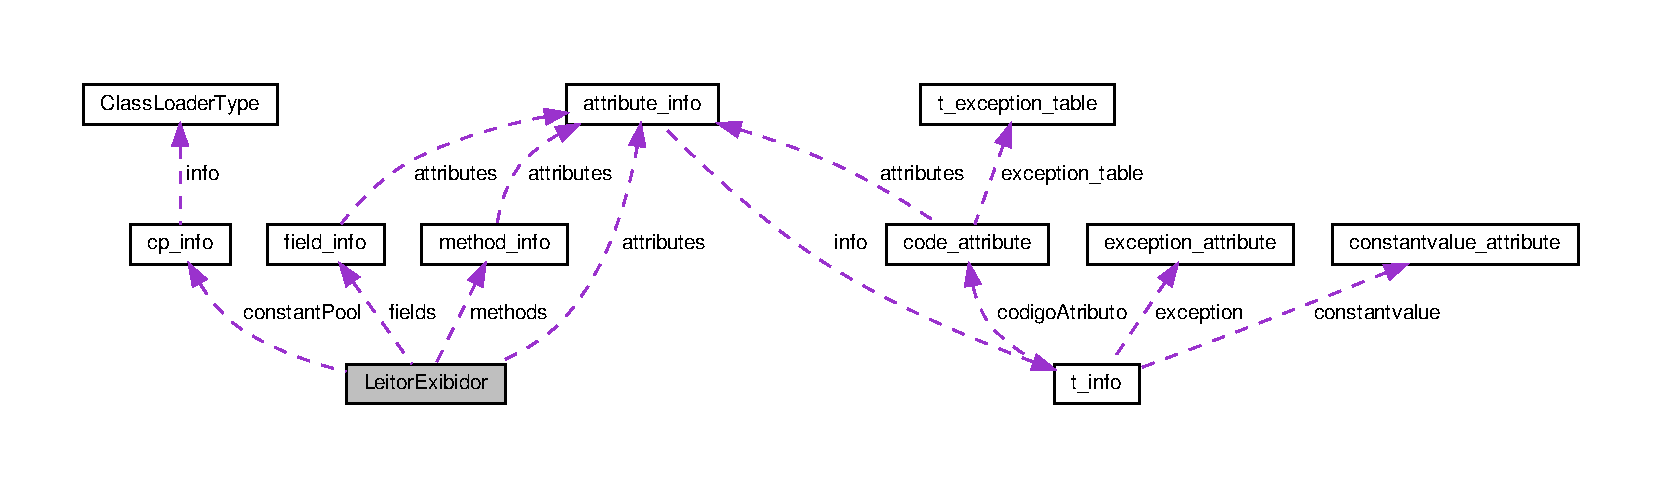
\includegraphics[width=350pt]{classLeitorExibidor__coll__graph}
\end{center}
\end{figure}
\subsection*{Membros públicos}
\begin{DoxyCompactItemize}
\item 
\hyperlink{classLeitorExibidor_aa1ffcfe21da762169b16483e4d30f683}{Leitor\+Exibidor} (char $\ast$in)
\begin{DoxyCompactList}\small\item\em Construtor que configura um objeto da classe \hyperlink{classLeitorExibidor}{Leitor\+Exibidor} com o nome do arquivo passado. \end{DoxyCompactList}\item 
\hyperlink{classLeitorExibidor_a10fd8d8b58be93148ff4d527c3ab5bd3}{Leitor\+Exibidor} (string in)
\begin{DoxyCompactList}\small\item\em Construtor que configura um objeto da classe \hyperlink{classLeitorExibidor}{Leitor\+Exibidor} com o nome do arquivo passado. \end{DoxyCompactList}\item 
int \hyperlink{classLeitorExibidor_a185520372593c9ee066d72c67e4a38e6}{inicializar\+Arquivo} (char $\ast$argv\mbox{[}$\,$\mbox{]})
\begin{DoxyCompactList}\small\item\em criar e inicializar arquivo \end{DoxyCompactList}\item 
void \hyperlink{classLeitorExibidor_a16868d53a83dca37586819aadeb7f0eb}{fechar\+Arquivo} ()
\begin{DoxyCompactList}\small\item\em Fechar arquivo. \end{DoxyCompactList}\item 
int \hyperlink{classLeitorExibidor_a493a9aed1941a4f01c611a2deeb37f8d}{carregar} ()
\item 
void \hyperlink{classLeitorExibidor_a338627a08235ffe50ede3d9e023c1238}{imprimir\+Informacoes\+Gerais} ()
\begin{DoxyCompactList}\small\item\em Imprime informações gerais do .class. \end{DoxyCompactList}\item 
void \hyperlink{classLeitorExibidor_ab65aba73916cc733df269b3033522a3c}{gravar\+Arquivo\+Informacoes\+Gerais} ()
\begin{DoxyCompactList}\small\item\em Gravar informações gerais do .class em um arquivo. \end{DoxyCompactList}\item 
bool \hyperlink{classLeitorExibidor_a544bd7574553d9015b22c2507971e7f5}{exibir} ()
\begin{DoxyCompactList}\small\item\em Imprime todas as informações do .class. \end{DoxyCompactList}\item 
bool \hyperlink{classLeitorExibidor_a8dcf6961e13ad6830f62e7839448b235}{gravar\+Arquivo} ()
\begin{DoxyCompactList}\small\item\em Gravar todas as informações do .class em um arquivo. \end{DoxyCompactList}\item 
bool \hyperlink{classLeitorExibidor_a83ed9ca5a7b4442ae3449daffc0d3d5c}{validar\+Extensao} ()
\begin{DoxyCompactList}\small\item\em Verifica se a extensão do arquivo é .class. \end{DoxyCompactList}\item 
bool \hyperlink{classLeitorExibidor_a431c625c01124f40e7b6f6fab2bdb7f2}{existe\+Main} ()
\begin{DoxyCompactList}\small\item\em Verifica se o .class possui função main. \end{DoxyCompactList}\item 
\hyperlink{structmethod__info}{method\+\_\+info} \hyperlink{classLeitorExibidor_a161f1cc97c2c71c800cf588f8a4eab67}{obter\+Main} ()
\begin{DoxyCompactList}\small\item\em Retorna o método main. \end{DoxyCompactList}\item 
bool \hyperlink{classLeitorExibidor_a5a3ef889b1e38506d9d0df17255cad4e}{existe\+Clinit} ()
\begin{DoxyCompactList}\small\item\em Verifica se o .class tem o método clinit. \end{DoxyCompactList}\item 
\hyperlink{structmethod__info}{method\+\_\+info} \hyperlink{classLeitorExibidor_a58636f719aebaaa46524233b94b46537}{obter\+Clinit} ()
\begin{DoxyCompactList}\small\item\em Retorna o método clinit. \end{DoxyCompactList}\item 
bool \hyperlink{classLeitorExibidor_a89d56b461514ed8fea8987ee52fa2eb9}{verificar\+This\+Class} ()
\begin{DoxyCompactList}\small\item\em Verifica se a class definida é igual ao nome da classe sem extensões. \end{DoxyCompactList}\item 
int \hyperlink{classLeitorExibidor_a6a9e55a1b824fed37f0841cb253789b2}{obter\+Status} ()
\begin{DoxyCompactList}\small\item\em Retorna o status lido, informando para o método que chamou o que aconteceu. \end{DoxyCompactList}\item 
\hyperlink{structcp__info}{cp\+\_\+info} $\ast$ \hyperlink{classLeitorExibidor_ab286b420bb915f3444ec78a003f4c25c}{obter\+Constant\+Pool} () const
\begin{DoxyCompactList}\small\item\em Retorna referencia a constant pool. \end{DoxyCompactList}\item 
\hyperlink{BasicTypes_8h_a90240657108b1b457eef9d3f76e0202e}{U2} \hyperlink{classLeitorExibidor_a7e64ad9d2b5f914f6bc4a0f84129f160}{obter\+Tamanho\+Constant\+Pool} ()
\begin{DoxyCompactList}\small\item\em Retorna o valor do tamanho da constant pool. \end{DoxyCompactList}\item 
char $\ast$ \hyperlink{classLeitorExibidor_a74785a29369d04d5a7d14ed63a0b2102}{obter\+Path} ()
\begin{DoxyCompactList}\small\item\em Pega o caminho do arquivo .class. \end{DoxyCompactList}\item 
\hyperlink{structmethod__info}{method\+\_\+info} $\ast$ \hyperlink{classLeitorExibidor_a0fbc8db7d08d00ec8f12e26bbce93048}{obter\+Methods} ()
\begin{DoxyCompactList}\small\item\em Retorna todos os métodos. \end{DoxyCompactList}\item 
\hyperlink{BasicTypes_8h_a90240657108b1b457eef9d3f76e0202e}{U2} \hyperlink{classLeitorExibidor_aa9c91f4a145f4ef753c33f8898075930}{obter\+Methods\+Count} ()
\begin{DoxyCompactList}\small\item\em Retorna o numero de Methods. \end{DoxyCompactList}\item 
\hyperlink{BasicTypes_8h_a90240657108b1b457eef9d3f76e0202e}{U2} \hyperlink{classLeitorExibidor_aa5cc18c3fb83811379d2f221980d8b8b}{obter\+This\+\_\+class} ()
\begin{DoxyCompactList}\small\item\em Retorna um índice da constant pool que aponta para string com nome da class. \end{DoxyCompactList}\item 
\hyperlink{BasicTypes_8h_a90240657108b1b457eef9d3f76e0202e}{U2} \hyperlink{classLeitorExibidor_ab46841a0392f45a35a5444dca234a1ae}{obter\+Super\+\_\+class} ()
\begin{DoxyCompactList}\small\item\em Retorna um índice da constant pool que aponta para string com nome da superclass. \end{DoxyCompactList}\item 
\hyperlink{BasicTypes_8h_a90240657108b1b457eef9d3f76e0202e}{U2} \hyperlink{classLeitorExibidor_a483e90f3d60c63a2b3d1106961c7f553}{obter\+Fields\+Count} ()
\begin{DoxyCompactList}\small\item\em Retorna número de fields. \end{DoxyCompactList}\item 
\hyperlink{structfield__info}{field\+\_\+info} $\ast$ \hyperlink{classLeitorExibidor_a480bbed0d19b7cf5d64753c9c1210464}{obter\+Fields} ()
\begin{DoxyCompactList}\small\item\em Retorna a array com as fields lidas. \end{DoxyCompactList}\item 
\hyperlink{structfield__info}{field\+\_\+info} $\ast$ \hyperlink{classLeitorExibidor_af51949669ace432f66221710ef3a3b00}{obter\+Field} (string nome)
\begin{DoxyCompactList}\small\item\em Retorna um field. \end{DoxyCompactList}\item 
\hyperlink{structmethod__info}{method\+\_\+info} $\ast$ \hyperlink{classLeitorExibidor_a4d1a48fa9825d2cb2b520be79112408c}{obter\+Method} (string nome, string descriptor)
\item 
\hyperlink{classLeitorExibidor}{Leitor\+Exibidor} $\ast$ \hyperlink{classLeitorExibidor_a3893e9478688cf21b293536da48f9f14}{obter\+Class\+That\+Has\+Serached\+Method} (string nome, string descriptor)
\begin{DoxyCompactList}\small\item\em Retorna o ponteiro para o leitor do .class que contém o método encontrado em get\+Method. \end{DoxyCompactList}\item 
int \hyperlink{classLeitorExibidor_a422272b830079ee349b468bbe78d4b13}{validacao} (void)
\begin{DoxyCompactList}\small\item\em Valida estrutura obrigatoria. \end{DoxyCompactList}\end{DoxyCompactItemize}
\subsection*{Membros privados}
\begin{DoxyCompactItemize}
\item 
bool \hyperlink{classLeitorExibidor_a2d486c9289a5d50a7fb00afffd2fa760}{verificar\+Main} ()
\begin{DoxyCompactList}\small\item\em Encontro em qual method está a main. \end{DoxyCompactList}\item 
bool \hyperlink{classLeitorExibidor_a8aeff3d072e77288215e5a070e958cf0}{verificar\+Clinit} ()
\begin{DoxyCompactList}\small\item\em Encontra em qual method esta a clinit, se existir. \end{DoxyCompactList}\item 
string \hyperlink{classLeitorExibidor_abf046987d5b3f0ec33794a547a8f9e25}{obter\+Erro} (int erro)
\begin{DoxyCompactList}\small\item\em Retorna a string que contém uma mensagem de erro correspondente ao índice que recebe como parâmetro. \end{DoxyCompactList}\end{DoxyCompactItemize}
\subsection*{Atributos Privados}
\begin{DoxyCompactItemize}
\item 
int \hyperlink{classLeitorExibidor_ac54b88860544d66f5e8f620c4c017a37}{status}
\item 
int \hyperlink{classLeitorExibidor_a9e7a108ebca3fac0096fcb422f2393db}{main\+Method}
\item 
int \hyperlink{classLeitorExibidor_a0c4c896a1baf647a282881524f8a9687}{clinit}
\item 
bool \hyperlink{classLeitorExibidor_aca32f682d0ccd1d60a76d0833ca0617f}{encontrou\+Main}
\item 
bool \hyperlink{classLeitorExibidor_a93a1aa14204f0445a97304cc504a3cf0}{encontrou\+Clinit}
\item 
char $\ast$ \hyperlink{classLeitorExibidor_a1dfa84388856ad4d83883e4e5548b485}{file\+Name}
\item 
\hyperlink{BasicTypes_8h_a90240657108b1b457eef9d3f76e0202e}{U2} \hyperlink{classLeitorExibidor_a6f6ac6ed85979359308c07c666316218}{min\+Version}
\item 
\hyperlink{BasicTypes_8h_a90240657108b1b457eef9d3f76e0202e}{U2} \hyperlink{classLeitorExibidor_a5c2cd58569e9c3fdc47c0bbab116b870}{maj\+Version}
\item 
\hyperlink{BasicTypes_8h_a90240657108b1b457eef9d3f76e0202e}{U2} \hyperlink{classLeitorExibidor_ae891dce6b86c2d09c1a112bd585561d6}{length\+CP}
\item 
\hyperlink{BasicTypes_8h_a90240657108b1b457eef9d3f76e0202e}{U2} \hyperlink{classLeitorExibidor_ad85a876f6368ae8101343f4f35b53019}{this\+\_\+class}
\item 
\hyperlink{BasicTypes_8h_a90240657108b1b457eef9d3f76e0202e}{U2} \hyperlink{classLeitorExibidor_adc9f3b119883f9bc4ba0323b8480c53e}{super\+\_\+class}
\item 
\hyperlink{BasicTypes_8h_a90240657108b1b457eef9d3f76e0202e}{U2} \hyperlink{classLeitorExibidor_a596a1440982d2418e39adf5b1857ab15}{interfaces\+Count}
\item 
\hyperlink{BasicTypes_8h_a90240657108b1b457eef9d3f76e0202e}{U2} \hyperlink{classLeitorExibidor_a9a54627d53b9a3c25c5ba71977e1e002}{fields\+Count}
\item 
\hyperlink{BasicTypes_8h_a90240657108b1b457eef9d3f76e0202e}{U2} \hyperlink{classLeitorExibidor_a3f5d59fb172e478ab6d1a595a8b6c54a}{methods\+Count}
\item 
\hyperlink{BasicTypes_8h_a90240657108b1b457eef9d3f76e0202e}{U2} \hyperlink{classLeitorExibidor_a16d6ecbc6b367cda3c0b774505285665}{access\+Flags}
\item 
\hyperlink{BasicTypes_8h_a90240657108b1b457eef9d3f76e0202e}{U2} \hyperlink{classLeitorExibidor_ac42b42a9a6c94c260db0016df94cda1d}{attributes\+Count}
\item 
\hyperlink{BasicTypes_8h_a90240657108b1b457eef9d3f76e0202e}{U2} $\ast$ \hyperlink{classLeitorExibidor_a7c19cc595c9d806b30477b5b008f3caa}{interfaces}
\item 
\hyperlink{structcp__info}{cp\+\_\+info} $\ast$ \hyperlink{classLeitorExibidor_ac92916cbf475e31ce0f2475d982ddaea}{constant\+Pool}
\item 
\hyperlink{structfield__info}{field\+\_\+info} $\ast$ \hyperlink{classLeitorExibidor_a6e8475e2db54d776db636c06d823eb3f}{fields}
\item 
\hyperlink{structmethod__info}{method\+\_\+info} $\ast$ \hyperlink{classLeitorExibidor_a0c9110ffe495c55bedaafdc47656eaed}{methods}
\item 
\hyperlink{structattribute__info}{attribute\+\_\+info} $\ast$ \hyperlink{classLeitorExibidor_adb26d0959bef738b08bffa009d12fac3}{attributes}
\item 
F\+I\+LE $\ast$ \hyperlink{classLeitorExibidor_acbb3d188113d55cc00b6e92bf2fddb98}{arquivo\+Class}
\item 
fstream \hyperlink{classLeitorExibidor_ae7f2edb9968df63470901712119e30d2}{arquivo\+Saida}
\end{DoxyCompactItemize}


\subsection{Descrição detalhada}
\hypertarget{classLeitorExibidor_DESCRIPTION}{}\subsection{D\+E\+S\+C\+R\+I\+P\+T\+I\+ON}\label{classLeitorExibidor_DESCRIPTION}
A classe \hyperlink{classLeitorExibidor}{Leitor\+Exibidor} contém o necessário para ler o bytecode, exibilo e armazena-\/lo em memoria 

Definido na linha 47 do ficheiro Classe\+Leitor\+Exibidor.\+h.



\subsection{Documentação dos Construtores \& Destrutor}
\mbox{\Hypertarget{classLeitorExibidor_aa1ffcfe21da762169b16483e4d30f683}\label{classLeitorExibidor_aa1ffcfe21da762169b16483e4d30f683}} 
\index{Leitor\+Exibidor@{Leitor\+Exibidor}!Leitor\+Exibidor@{Leitor\+Exibidor}}
\index{Leitor\+Exibidor@{Leitor\+Exibidor}!Leitor\+Exibidor@{Leitor\+Exibidor}}
\subsubsection{\texorpdfstring{Leitor\+Exibidor()}{LeitorExibidor()}\hspace{0.1cm}{\footnotesize\ttfamily [1/2]}}
{\footnotesize\ttfamily Leitor\+Exibidor\+::\+Leitor\+Exibidor (\begin{DoxyParamCaption}\item[{char $\ast$}]{in }\end{DoxyParamCaption})}



Construtor que configura um objeto da classe \hyperlink{classLeitorExibidor}{Leitor\+Exibidor} com o nome do arquivo passado. 


\begin{DoxyParams}{Parâmetros}
{\em in} & caminho do arquivo .class. \\
\hline
\end{DoxyParams}


Definido na linha 8 do ficheiro Classe\+Leitor\+Exibidor.\+cpp.



Referências file\+Name e status.

\mbox{\Hypertarget{classLeitorExibidor_a10fd8d8b58be93148ff4d527c3ab5bd3}\label{classLeitorExibidor_a10fd8d8b58be93148ff4d527c3ab5bd3}} 
\index{Leitor\+Exibidor@{Leitor\+Exibidor}!Leitor\+Exibidor@{Leitor\+Exibidor}}
\index{Leitor\+Exibidor@{Leitor\+Exibidor}!Leitor\+Exibidor@{Leitor\+Exibidor}}
\subsubsection{\texorpdfstring{Leitor\+Exibidor()}{LeitorExibidor()}\hspace{0.1cm}{\footnotesize\ttfamily [2/2]}}
{\footnotesize\ttfamily Leitor\+Exibidor\+::\+Leitor\+Exibidor (\begin{DoxyParamCaption}\item[{string}]{in }\end{DoxyParamCaption})}



Construtor que configura um objeto da classe \hyperlink{classLeitorExibidor}{Leitor\+Exibidor} com o nome do arquivo passado. 


\begin{DoxyParams}{Parâmetros}
{\em in} & caminho do arquivo .class. \\
\hline
\end{DoxyParams}


Definido na linha 15 do ficheiro Classe\+Leitor\+Exibidor.\+cpp.



Referências file\+Name e status.



\subsection{Documentação dos métodos}
\mbox{\Hypertarget{classLeitorExibidor_a493a9aed1941a4f01c611a2deeb37f8d}\label{classLeitorExibidor_a493a9aed1941a4f01c611a2deeb37f8d}} 
\index{Leitor\+Exibidor@{Leitor\+Exibidor}!carregar@{carregar}}
\index{carregar@{carregar}!Leitor\+Exibidor@{Leitor\+Exibidor}}
\subsubsection{\texorpdfstring{carregar()}{carregar()}}
{\footnotesize\ttfamily int Leitor\+Exibidor\+::carregar (\begin{DoxyParamCaption}{ }\end{DoxyParamCaption})}

Carrega o class file na classe \begin{DoxyReturn}{Retorna}
variavel status que indica se houve erro no programa 
\end{DoxyReturn}


Definido na linha 68 do ficheiro Classe\+Leitor\+Exibidor.\+cpp.



Referências access\+Flags, arquivo\+Class, attributes, attributes\+Count, C\+A\+N\+T\+\_\+\+O\+P\+EN, carregar\+Constant\+Pool(), constant\+Pool, encontrou\+Clinit, encontrou\+Main, fields, fields\+Count, file\+Name, interfaces, interfaces\+Count, I\+N\+V\+A\+L\+I\+D\+\_\+\+E\+X\+T\+E\+N\+S\+I\+ON, I\+N\+V\+A\+L\+I\+D\+\_\+\+F\+I\+LE, I\+N\+V\+A\+L\+I\+D\+\_\+\+N\+A\+ME, length\+CP, ler\+Todas\+Interfaces(), ler\+Todos\+Attributes(), ler\+Todos\+Fields(), ler\+Todos\+Methods(), ler\+U2(), ler\+U4(), maj\+Version, methods, methods\+Count, min\+Version, M\+I\+S\+S\+I\+N\+G\+\_\+\+A\+R\+G\+U\+M\+E\+NT, obter\+Erro(), status, super\+\_\+class, this\+\_\+class, U\+N\+K\+N\+O\+W\+N\+\_\+\+T\+Y\+PE, validar\+Extensao(), verificar\+Clinit(), verificar\+Main() e verificar\+This\+Class().



Referenciado por Method\+Area\+::adicionar\+Classe() e main().

Grafo de chamadas desta função\+:
\nopagebreak
\begin{figure}[H]
\begin{center}
\leavevmode
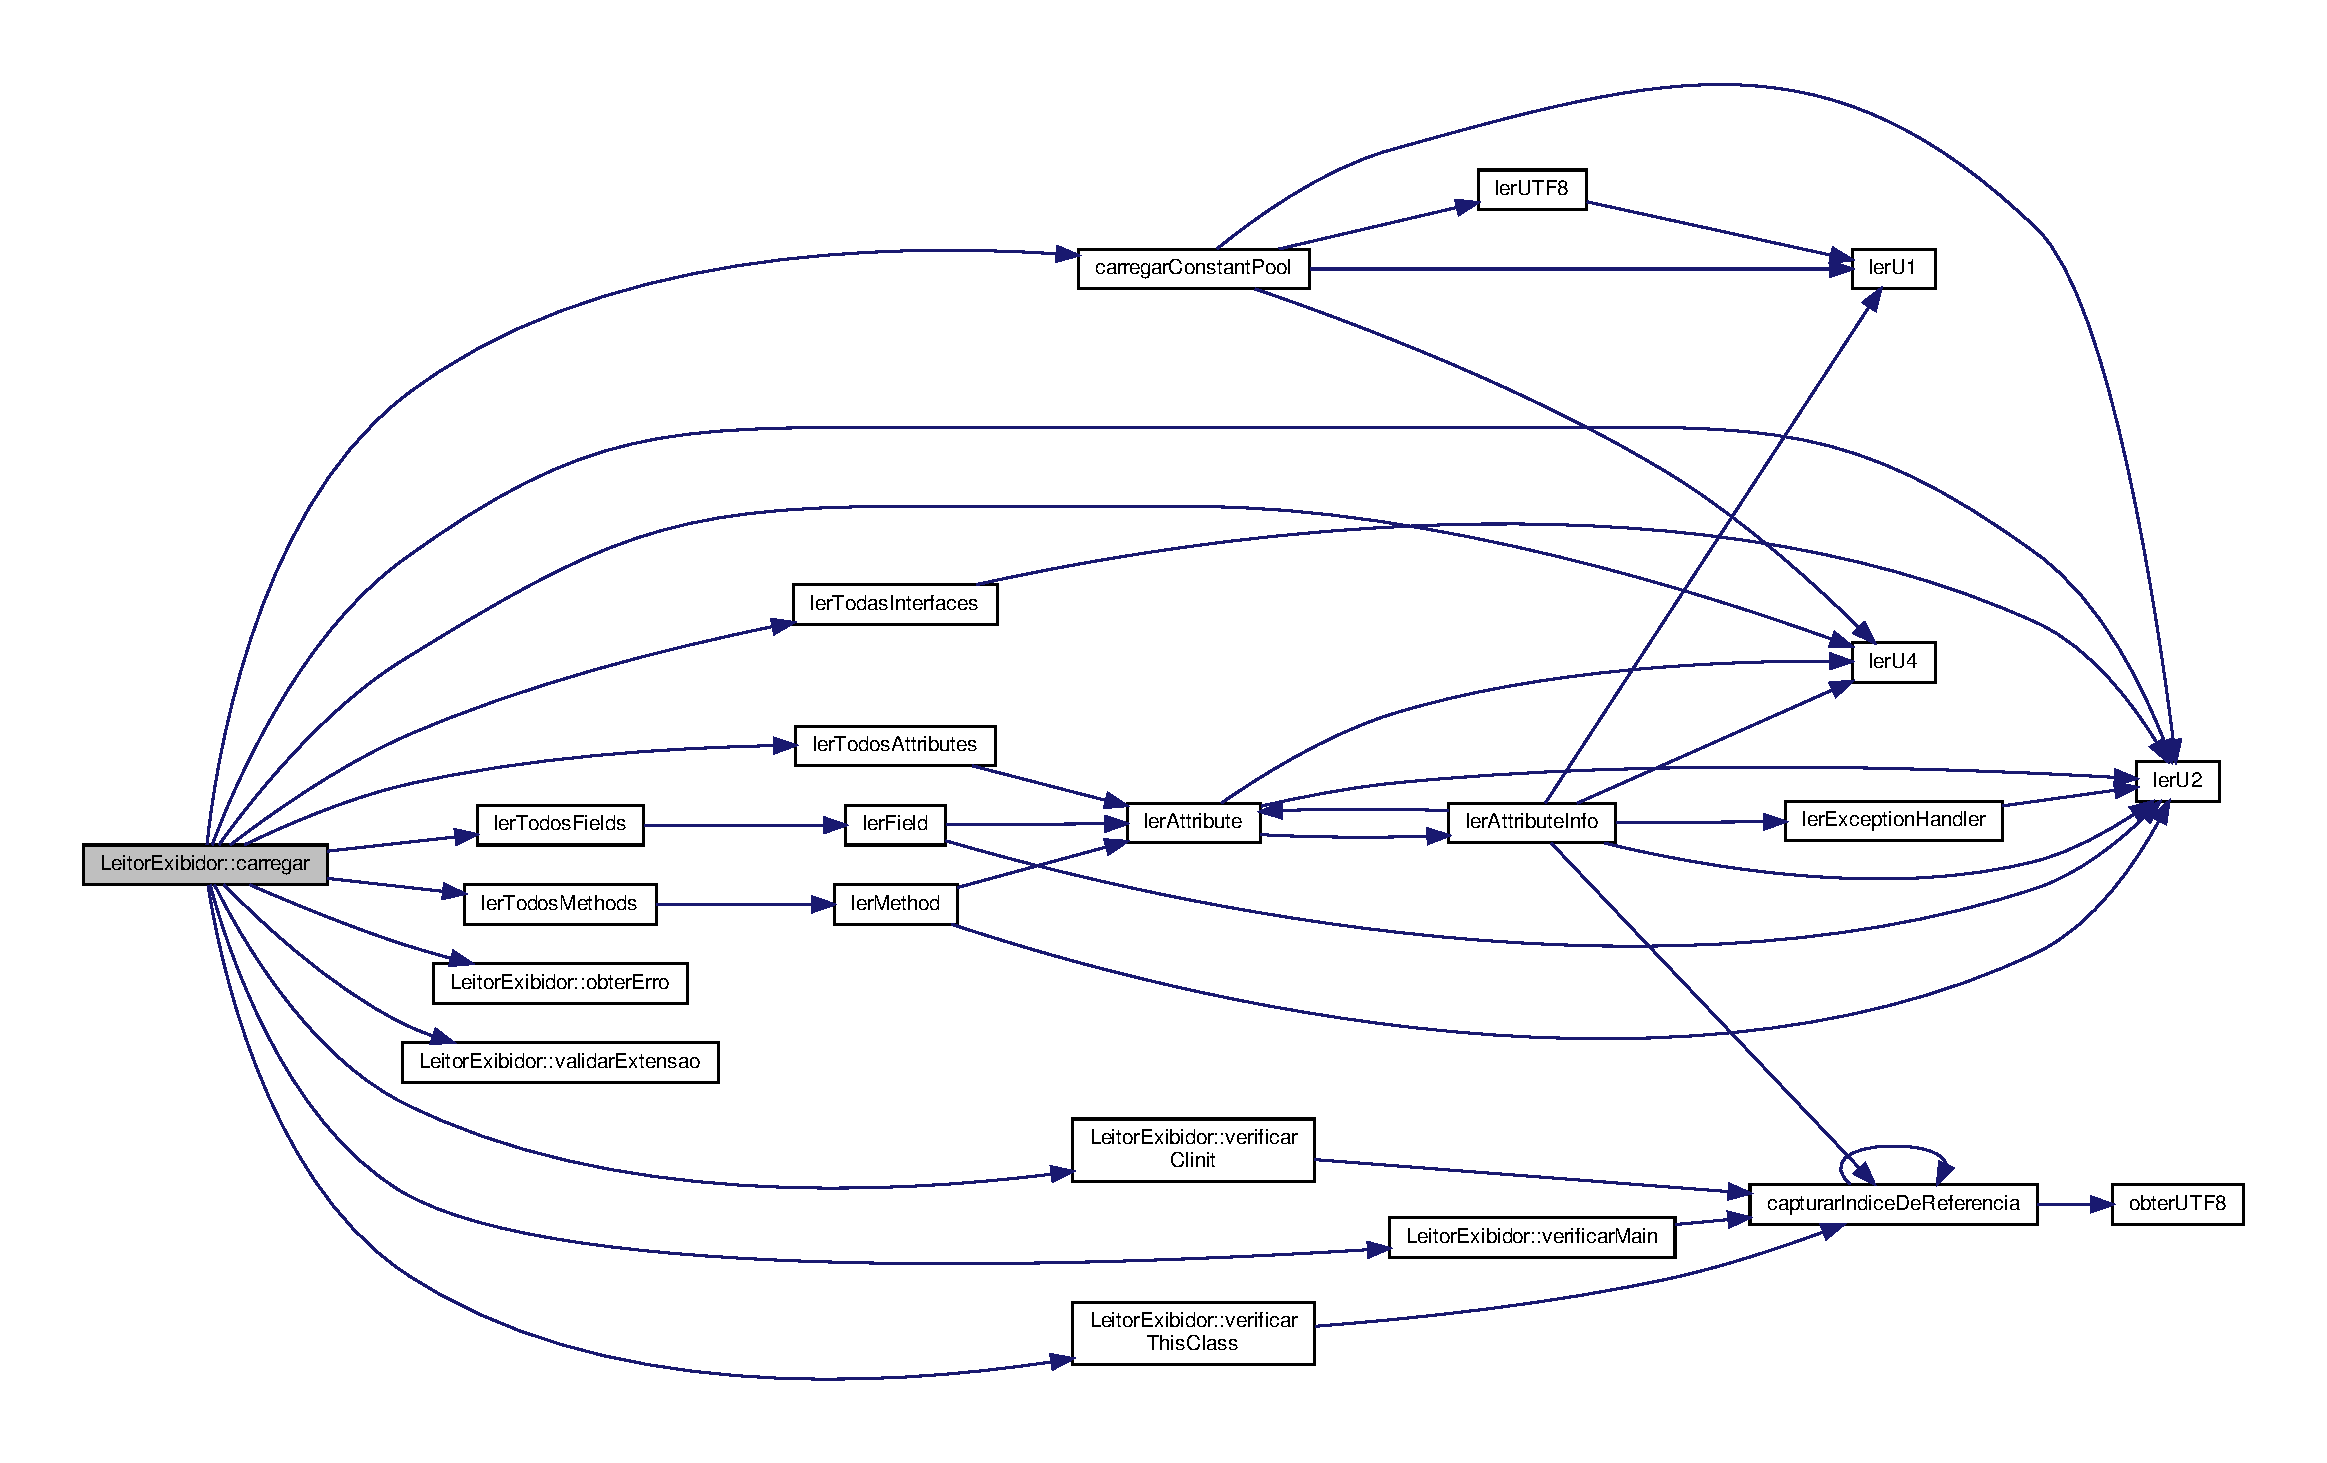
\includegraphics[width=350pt]{classLeitorExibidor_a493a9aed1941a4f01c611a2deeb37f8d_cgraph}
\end{center}
\end{figure}
\mbox{\Hypertarget{classLeitorExibidor_a544bd7574553d9015b22c2507971e7f5}\label{classLeitorExibidor_a544bd7574553d9015b22c2507971e7f5}} 
\index{Leitor\+Exibidor@{Leitor\+Exibidor}!exibir@{exibir}}
\index{exibir@{exibir}!Leitor\+Exibidor@{Leitor\+Exibidor}}
\subsubsection{\texorpdfstring{exibir()}{exibir()}}
{\footnotesize\ttfamily bool Leitor\+Exibidor\+::exibir (\begin{DoxyParamCaption}{ }\end{DoxyParamCaption})}



Imprime todas as informações do .class. 

\begin{DoxyReturn}{Retorna}
true ou false dependendo se a variavel status indicar que houve erro na leitura 
\end{DoxyReturn}


Definido na linha 176 do ficheiro Classe\+Leitor\+Exibidor.\+cpp.



Referências attributes, attributes\+Count, constant\+Pool, fields, fields\+Count, imprimir\+Constant\+Pool(), imprimir\+Informacoes\+Gerais(), imprimir\+Todas\+Interfaces(), imprimir\+Todos\+Attributes(), imprimir\+Todos\+Field(), imprimir\+Todos\+Methods(), interfaces, interfaces\+Count, length\+CP, methods, methods\+Count e status.



Referenciado por main().

Grafo de chamadas desta função\+:
\nopagebreak
\begin{figure}[H]
\begin{center}
\leavevmode
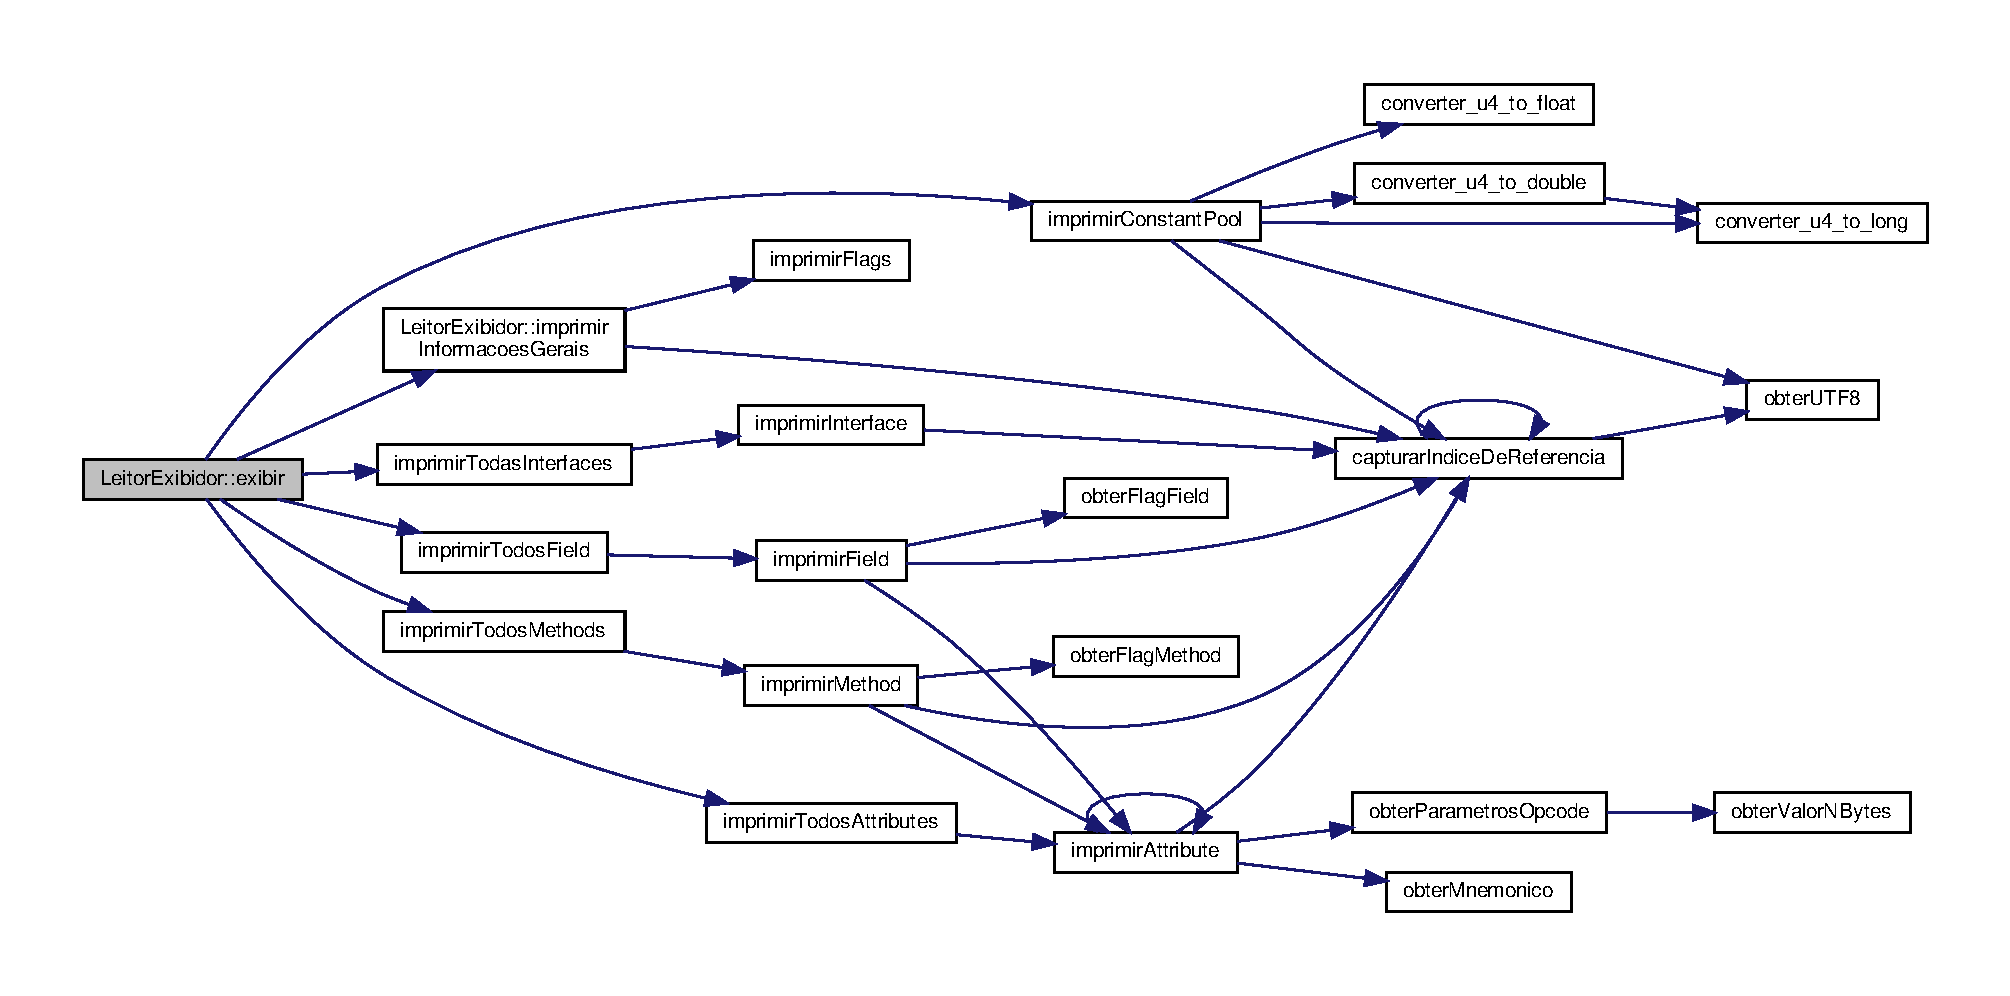
\includegraphics[width=350pt]{classLeitorExibidor_a544bd7574553d9015b22c2507971e7f5_cgraph}
\end{center}
\end{figure}
\mbox{\Hypertarget{classLeitorExibidor_a5a3ef889b1e38506d9d0df17255cad4e}\label{classLeitorExibidor_a5a3ef889b1e38506d9d0df17255cad4e}} 
\index{Leitor\+Exibidor@{Leitor\+Exibidor}!existe\+Clinit@{existe\+Clinit}}
\index{existe\+Clinit@{existe\+Clinit}!Leitor\+Exibidor@{Leitor\+Exibidor}}
\subsubsection{\texorpdfstring{existe\+Clinit()}{existeClinit()}}
{\footnotesize\ttfamily bool Leitor\+Exibidor\+::existe\+Clinit (\begin{DoxyParamCaption}{ }\end{DoxyParamCaption})}



Verifica se o .class tem o método clinit. 

\begin{DoxyReturn}{Retorna}
booleano que indica se existe o metodo clinit 
\end{DoxyReturn}


Definido na linha 344 do ficheiro Classe\+Leitor\+Exibidor.\+cpp.



Referências encontrou\+Clinit e verificar\+Clinit().



Referenciado por Method\+Area\+::adicionar\+Classe().

Grafo de chamadas desta função\+:
\nopagebreak
\begin{figure}[H]
\begin{center}
\leavevmode
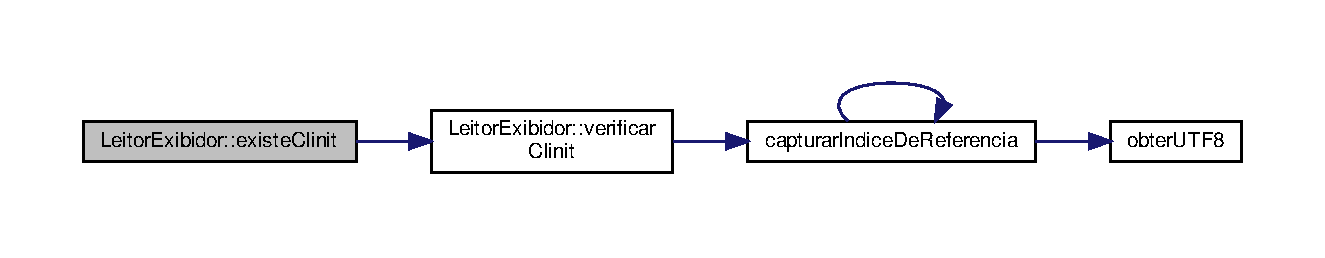
\includegraphics[width=350pt]{classLeitorExibidor_a5a3ef889b1e38506d9d0df17255cad4e_cgraph}
\end{center}
\end{figure}
\mbox{\Hypertarget{classLeitorExibidor_a431c625c01124f40e7b6f6fab2bdb7f2}\label{classLeitorExibidor_a431c625c01124f40e7b6f6fab2bdb7f2}} 
\index{Leitor\+Exibidor@{Leitor\+Exibidor}!existe\+Main@{existe\+Main}}
\index{existe\+Main@{existe\+Main}!Leitor\+Exibidor@{Leitor\+Exibidor}}
\subsubsection{\texorpdfstring{existe\+Main()}{existeMain()}}
{\footnotesize\ttfamily bool Leitor\+Exibidor\+::existe\+Main (\begin{DoxyParamCaption}{ }\end{DoxyParamCaption})}



Verifica se o .class possui função main. 

\begin{DoxyReturn}{Retorna}
booleano que indica se existe o metodo main 
\end{DoxyReturn}


Definido na linha 338 do ficheiro Classe\+Leitor\+Exibidor.\+cpp.



Referências encontrou\+Main e verificar\+Main().

Grafo de chamadas desta função\+:
\nopagebreak
\begin{figure}[H]
\begin{center}
\leavevmode
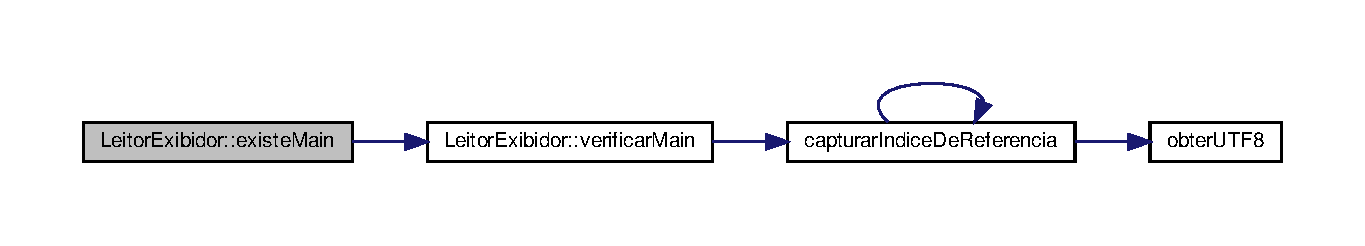
\includegraphics[width=350pt]{classLeitorExibidor_a431c625c01124f40e7b6f6fab2bdb7f2_cgraph}
\end{center}
\end{figure}
\mbox{\Hypertarget{classLeitorExibidor_a16868d53a83dca37586819aadeb7f0eb}\label{classLeitorExibidor_a16868d53a83dca37586819aadeb7f0eb}} 
\index{Leitor\+Exibidor@{Leitor\+Exibidor}!fechar\+Arquivo@{fechar\+Arquivo}}
\index{fechar\+Arquivo@{fechar\+Arquivo}!Leitor\+Exibidor@{Leitor\+Exibidor}}
\subsubsection{\texorpdfstring{fechar\+Arquivo()}{fecharArquivo()}}
{\footnotesize\ttfamily void Leitor\+Exibidor\+::fechar\+Arquivo (\begin{DoxyParamCaption}{ }\end{DoxyParamCaption})}



Fechar arquivo. 



Definido na linha 41 do ficheiro Classe\+Leitor\+Exibidor.\+cpp.



Referências arquivo\+Saida.



Referenciado por main().

\mbox{\Hypertarget{classLeitorExibidor_a8dcf6961e13ad6830f62e7839448b235}\label{classLeitorExibidor_a8dcf6961e13ad6830f62e7839448b235}} 
\index{Leitor\+Exibidor@{Leitor\+Exibidor}!gravar\+Arquivo@{gravar\+Arquivo}}
\index{gravar\+Arquivo@{gravar\+Arquivo}!Leitor\+Exibidor@{Leitor\+Exibidor}}
\subsubsection{\texorpdfstring{gravar\+Arquivo()}{gravarArquivo()}}
{\footnotesize\ttfamily bool Leitor\+Exibidor\+::gravar\+Arquivo (\begin{DoxyParamCaption}{ }\end{DoxyParamCaption})}



Gravar todas as informações do .class em um arquivo. 

\begin{DoxyReturn}{Retorna}
true ou false dependendo se a variavel status indicar que houve erro na leitura 
\end{DoxyReturn}


Definido na linha 203 do ficheiro Classe\+Leitor\+Exibidor.\+cpp.



Referências arquivo\+Saida, attributes, attributes\+Count, constant\+Pool, fields, fields\+Count, gravar\+Arquivo\+Constant\+Pool(), gravar\+Arquivo\+Informacoes\+Gerais(), gravar\+Arquivo\+Todas\+Interfaces(), gravar\+Arquivo\+Todos\+Attributes(), gravar\+Arquivo\+Todos\+Field(), gravar\+Arquivo\+Todos\+Methods(), interfaces, interfaces\+Count, length\+CP, methods, methods\+Count e status.



Referenciado por main().

Grafo de chamadas desta função\+:
\nopagebreak
\begin{figure}[H]
\begin{center}
\leavevmode
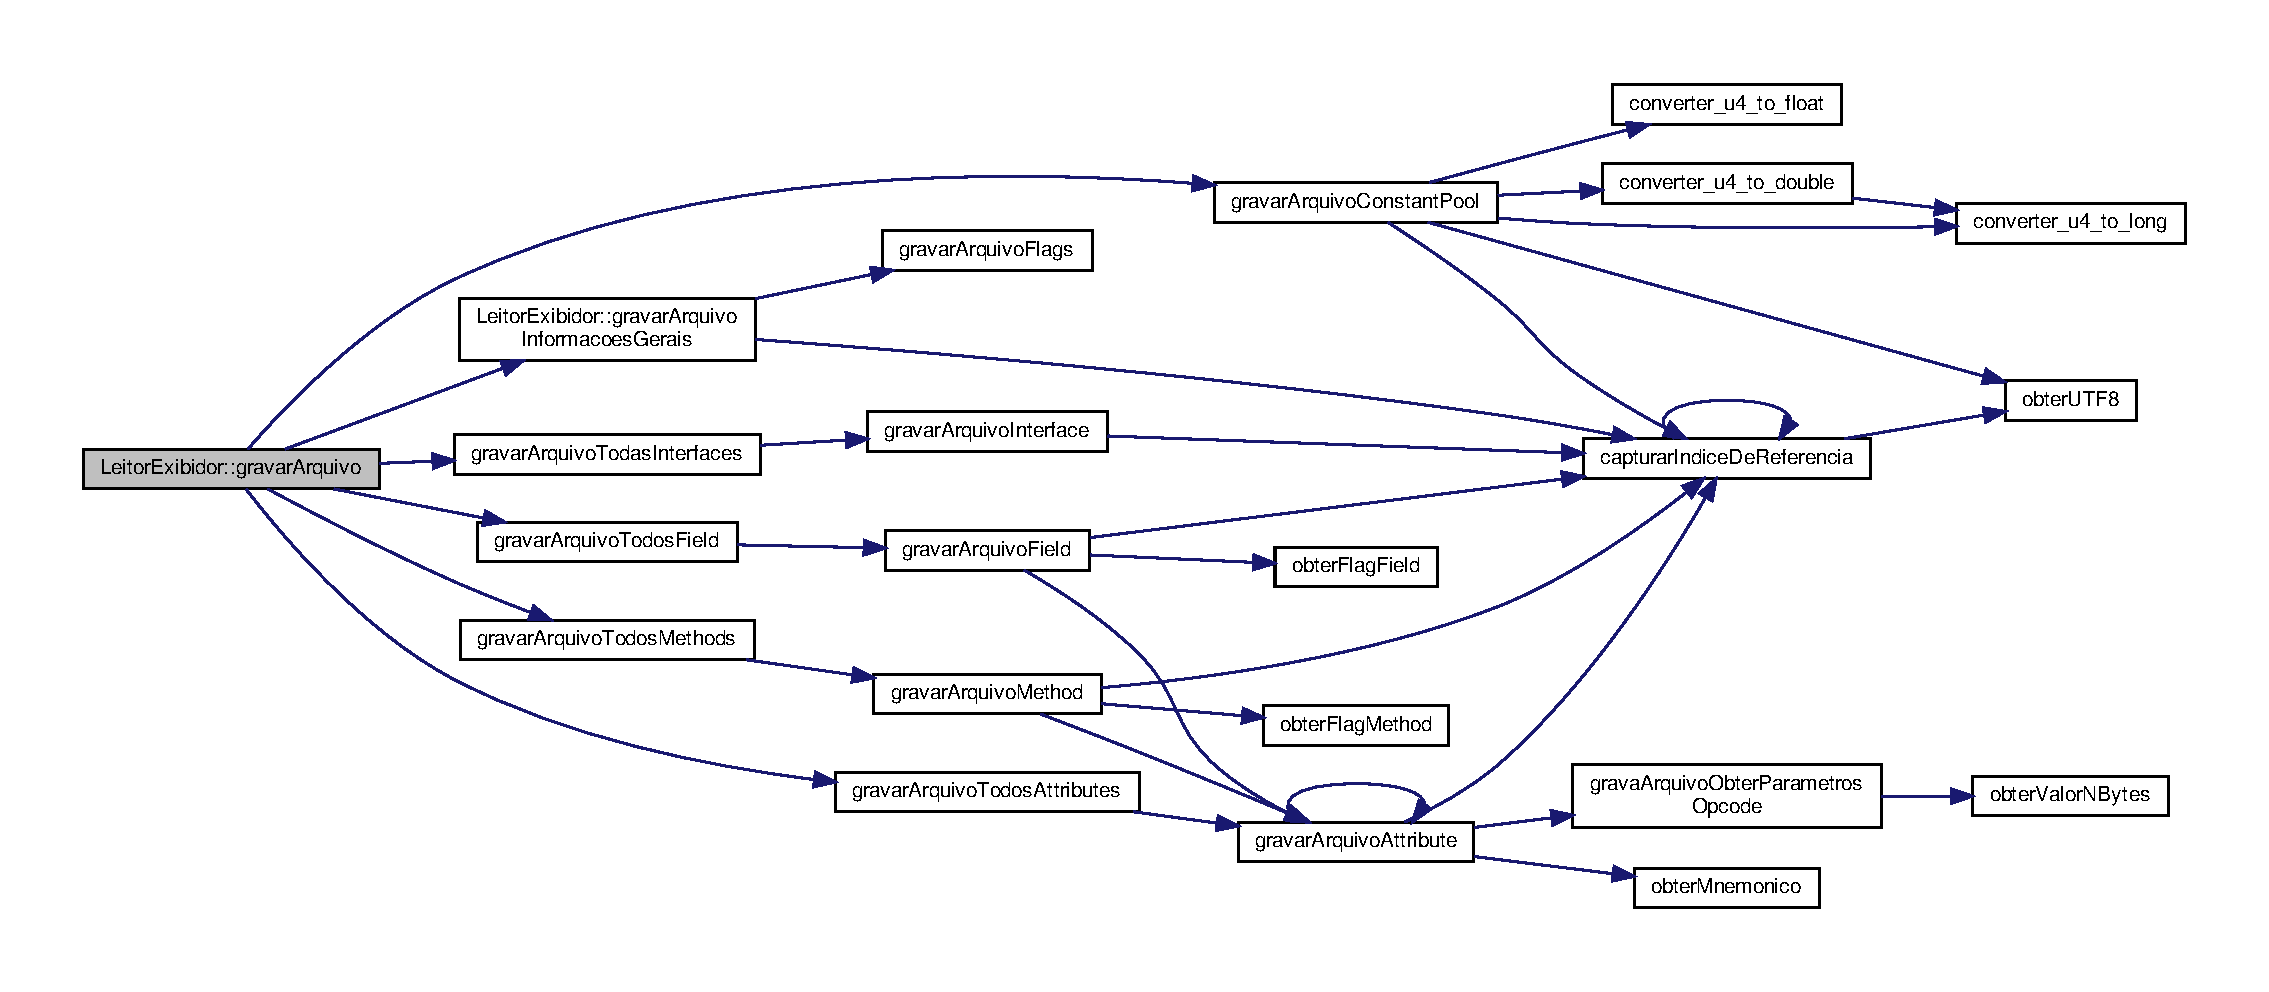
\includegraphics[width=350pt]{classLeitorExibidor_a8dcf6961e13ad6830f62e7839448b235_cgraph}
\end{center}
\end{figure}
\mbox{\Hypertarget{classLeitorExibidor_ab65aba73916cc733df269b3033522a3c}\label{classLeitorExibidor_ab65aba73916cc733df269b3033522a3c}} 
\index{Leitor\+Exibidor@{Leitor\+Exibidor}!gravar\+Arquivo\+Informacoes\+Gerais@{gravar\+Arquivo\+Informacoes\+Gerais}}
\index{gravar\+Arquivo\+Informacoes\+Gerais@{gravar\+Arquivo\+Informacoes\+Gerais}!Leitor\+Exibidor@{Leitor\+Exibidor}}
\subsubsection{\texorpdfstring{gravar\+Arquivo\+Informacoes\+Gerais()}{gravarArquivoInformacoesGerais()}}
{\footnotesize\ttfamily bool Leitor\+Exibidor\+::gravar\+Arquivo\+Informacoes\+Gerais (\begin{DoxyParamCaption}{ }\end{DoxyParamCaption})}



Gravar informações gerais do .class em um arquivo. 

\begin{DoxyReturn}{Retorna}
variavel status que indica se houve erro no programa 
\end{DoxyReturn}


Definido na linha 253 do ficheiro Classe\+Leitor\+Exibidor.\+cpp.



Referências access\+Flags, arquivo\+Saida, attributes\+Count, capturar\+Indice\+De\+Referencia(), constant\+Pool, fields\+Count, gravar\+Arquivo\+Flags(), interfaces\+Count, length\+CP, maj\+Version, methods\+Count, min\+Version, super\+\_\+class e this\+\_\+class.



Referenciado por gravar\+Arquivo().

Grafo de chamadas desta função\+:
\nopagebreak
\begin{figure}[H]
\begin{center}
\leavevmode
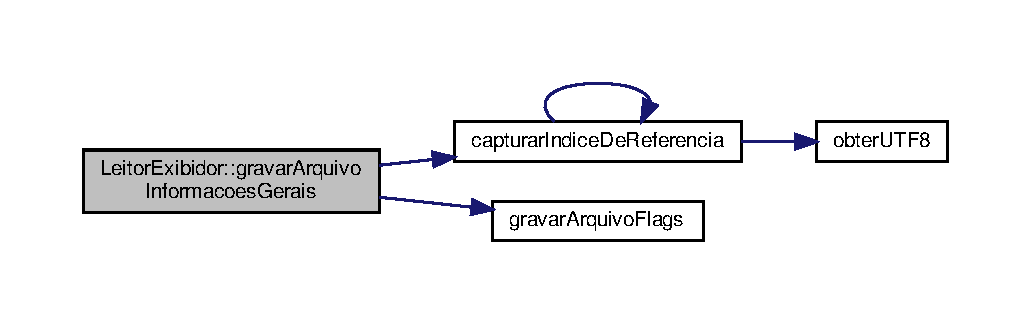
\includegraphics[width=350pt]{classLeitorExibidor_ab65aba73916cc733df269b3033522a3c_cgraph}
\end{center}
\end{figure}
\mbox{\Hypertarget{classLeitorExibidor_a338627a08235ffe50ede3d9e023c1238}\label{classLeitorExibidor_a338627a08235ffe50ede3d9e023c1238}} 
\index{Leitor\+Exibidor@{Leitor\+Exibidor}!imprimir\+Informacoes\+Gerais@{imprimir\+Informacoes\+Gerais}}
\index{imprimir\+Informacoes\+Gerais@{imprimir\+Informacoes\+Gerais}!Leitor\+Exibidor@{Leitor\+Exibidor}}
\subsubsection{\texorpdfstring{imprimir\+Informacoes\+Gerais()}{imprimirInformacoesGerais()}}
{\footnotesize\ttfamily bool Leitor\+Exibidor\+::imprimir\+Informacoes\+Gerais (\begin{DoxyParamCaption}{ }\end{DoxyParamCaption})}



Imprime informações gerais do .class. 

\begin{DoxyReturn}{Retorna}
variavel status que indica se houve erro no programa 
\end{DoxyReturn}


Definido na linha 224 do ficheiro Classe\+Leitor\+Exibidor.\+cpp.



Referências access\+Flags, attributes\+Count, capturar\+Indice\+De\+Referencia(), constant\+Pool, fields\+Count, imprimir\+Flags(), interfaces\+Count, length\+CP, maj\+Version, methods\+Count, min\+Version, super\+\_\+class e this\+\_\+class.



Referenciado por exibir().

Grafo de chamadas desta função\+:
\nopagebreak
\begin{figure}[H]
\begin{center}
\leavevmode
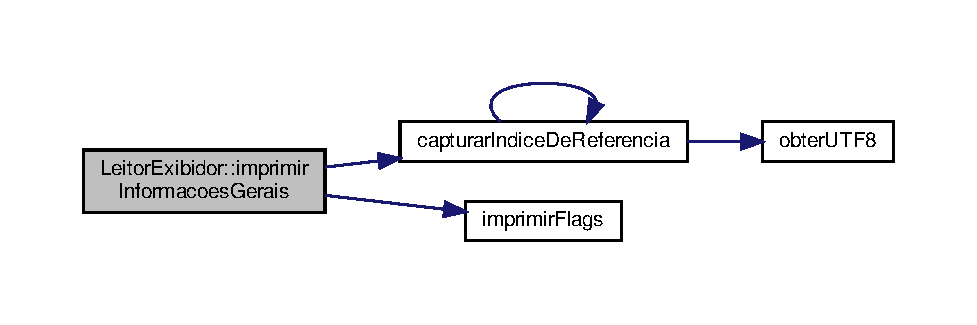
\includegraphics[width=350pt]{classLeitorExibidor_a338627a08235ffe50ede3d9e023c1238_cgraph}
\end{center}
\end{figure}
\mbox{\Hypertarget{classLeitorExibidor_a185520372593c9ee066d72c67e4a38e6}\label{classLeitorExibidor_a185520372593c9ee066d72c67e4a38e6}} 
\index{Leitor\+Exibidor@{Leitor\+Exibidor}!inicializar\+Arquivo@{inicializar\+Arquivo}}
\index{inicializar\+Arquivo@{inicializar\+Arquivo}!Leitor\+Exibidor@{Leitor\+Exibidor}}
\subsubsection{\texorpdfstring{inicializar\+Arquivo()}{inicializarArquivo()}}
{\footnotesize\ttfamily int Leitor\+Exibidor\+::inicializar\+Arquivo (\begin{DoxyParamCaption}\item[{char $\ast$}]{argv\mbox{[}$\,$\mbox{]} }\end{DoxyParamCaption})}



criar e inicializar arquivo 



Definido na linha 27 do ficheiro Classe\+Leitor\+Exibidor.\+cpp.



Referências arquivo\+Saida e status.



Referenciado por main().

\mbox{\Hypertarget{classLeitorExibidor_a3893e9478688cf21b293536da48f9f14}\label{classLeitorExibidor_a3893e9478688cf21b293536da48f9f14}} 
\index{Leitor\+Exibidor@{Leitor\+Exibidor}!obter\+Class\+That\+Has\+Serached\+Method@{obter\+Class\+That\+Has\+Serached\+Method}}
\index{obter\+Class\+That\+Has\+Serached\+Method@{obter\+Class\+That\+Has\+Serached\+Method}!Leitor\+Exibidor@{Leitor\+Exibidor}}
\subsubsection{\texorpdfstring{obter\+Class\+That\+Has\+Serached\+Method()}{obterClassThatHasSerachedMethod()}}
{\footnotesize\ttfamily \hyperlink{classLeitorExibidor}{Leitor\+Exibidor} $\ast$ Leitor\+Exibidor\+::obter\+Class\+That\+Has\+Serached\+Method (\begin{DoxyParamCaption}\item[{string}]{nome,  }\item[{string}]{descriptor }\end{DoxyParamCaption})}



Retorna o ponteiro para o leitor do .class que contém o método encontrado em get\+Method. 


\begin{DoxyParams}{Parâmetros}
{\em nome} & Nome do method desejado \\
\hline
{\em descriptor} & Descritor do method desejado \\
\hline
\end{DoxyParams}
\begin{DoxyReturn}{Retorna}
classe \hyperlink{classLeitorExibidor}{Leitor\+Exibidor} 
\end{DoxyReturn}


Definido na linha 538 do ficheiro Classe\+Leitor\+Exibidor.\+cpp.



Referências capturar\+Indice\+De\+Referencia(), constant\+Pool, method\+\_\+info\+::descriptor\+\_\+index, methods, methods\+Count, method\+\_\+info\+::name\+\_\+index, Method\+Area\+::obter\+Class(), Static\+Class\+::obter\+Classe\+Leitor\+Exibidor(), obter\+Class\+That\+Has\+Serached\+Method() e obter\+Super\+\_\+class().



Referenciado por Operations\+::invokeinterface(), Operations\+::invokespecial(), Operations\+::invokestatic(), Operations\+::invokevirtual() e obter\+Class\+That\+Has\+Serached\+Method().

Grafo de chamadas desta função\+:
\nopagebreak
\begin{figure}[H]
\begin{center}
\leavevmode
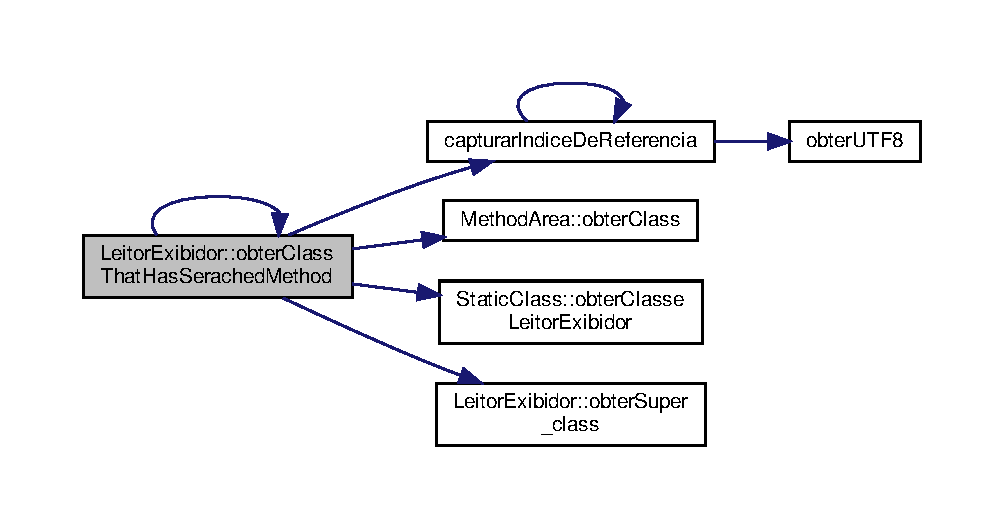
\includegraphics[width=350pt]{classLeitorExibidor_a3893e9478688cf21b293536da48f9f14_cgraph}
\end{center}
\end{figure}
\mbox{\Hypertarget{classLeitorExibidor_a58636f719aebaaa46524233b94b46537}\label{classLeitorExibidor_a58636f719aebaaa46524233b94b46537}} 
\index{Leitor\+Exibidor@{Leitor\+Exibidor}!obter\+Clinit@{obter\+Clinit}}
\index{obter\+Clinit@{obter\+Clinit}!Leitor\+Exibidor@{Leitor\+Exibidor}}
\subsubsection{\texorpdfstring{obter\+Clinit()}{obterClinit()}}
{\footnotesize\ttfamily \hyperlink{structmethod__info}{method\+\_\+info} Leitor\+Exibidor\+::obter\+Clinit (\begin{DoxyParamCaption}{ }\end{DoxyParamCaption})}



Retorna o método clinit. 

\begin{DoxyReturn}{Retorna}
struct \hyperlink{structmethod__info}{method\+\_\+info} contendo informações sobre o método 
\end{DoxyReturn}


Definido na linha 358 do ficheiro Classe\+Leitor\+Exibidor.\+cpp.



Referências clinit e methods.



Referenciado por Method\+Area\+::adicionar\+Classe().

\mbox{\Hypertarget{classLeitorExibidor_ab286b420bb915f3444ec78a003f4c25c}\label{classLeitorExibidor_ab286b420bb915f3444ec78a003f4c25c}} 
\index{Leitor\+Exibidor@{Leitor\+Exibidor}!obter\+Constant\+Pool@{obter\+Constant\+Pool}}
\index{obter\+Constant\+Pool@{obter\+Constant\+Pool}!Leitor\+Exibidor@{Leitor\+Exibidor}}
\subsubsection{\texorpdfstring{obter\+Constant\+Pool()}{obterConstantPool()}}
{\footnotesize\ttfamily \hyperlink{structcp__info}{cp\+\_\+info} $\ast$ Leitor\+Exibidor\+::obter\+Constant\+Pool (\begin{DoxyParamCaption}{ }\end{DoxyParamCaption}) const}



Retorna referencia a constant pool. 

\begin{DoxyReturn}{Retorna}
Retorna a array com a constant pool 
\end{DoxyReturn}


Definido na linha 441 do ficheiro Classe\+Leitor\+Exibidor.\+cpp.



Referências constant\+Pool.



Referenciado por Method\+Area\+::adicionar\+Classe(), Frame\+Stack\+::\+Frame\+Stack(), Instance\+Class\+::\+Instance\+Class(), Operations\+::invokeinterface(), Operations\+::invokespecial(), Operations\+::invokestatic(), Operations\+::invokevirtual(), Operations\+::obter\+Static\+Class\+That\+Has\+Field() e Static\+Class\+::\+Static\+Class().

\mbox{\Hypertarget{classLeitorExibidor_abf046987d5b3f0ec33794a547a8f9e25}\label{classLeitorExibidor_abf046987d5b3f0ec33794a547a8f9e25}} 
\index{Leitor\+Exibidor@{Leitor\+Exibidor}!obter\+Erro@{obter\+Erro}}
\index{obter\+Erro@{obter\+Erro}!Leitor\+Exibidor@{Leitor\+Exibidor}}
\subsubsection{\texorpdfstring{obter\+Erro()}{obterErro()}}
{\footnotesize\ttfamily string Leitor\+Exibidor\+::obter\+Erro (\begin{DoxyParamCaption}\item[{int}]{erro }\end{DoxyParamCaption})\hspace{0.3cm}{\ttfamily [private]}}



Retorna a string que contém uma mensagem de erro correspondente ao índice que recebe como parâmetro. 


\begin{DoxyParams}{Parâmetros}
{\em erro} & M\+A\+C\+RO com o erro que foi encontrado \\
\hline
\end{DoxyParams}
\begin{DoxyReturn}{Retorna}
string contendo informação sobre o tipo de erro encontrado 
\end{DoxyReturn}


Definido na linha 408 do ficheiro Classe\+Leitor\+Exibidor.\+cpp.



Referências C\+A\+N\+T\+\_\+\+O\+P\+EN, file\+Name, I\+N\+V\+A\+L\+I\+D\+\_\+\+E\+X\+T\+E\+N\+S\+I\+ON, I\+N\+V\+A\+L\+I\+D\+\_\+\+F\+I\+LE, I\+N\+V\+A\+L\+I\+D\+\_\+\+N\+A\+ME, M\+I\+S\+S\+I\+N\+G\+\_\+\+A\+R\+G\+U\+M\+E\+NT, M\+I\+S\+S\+I\+N\+G\+\_\+\+C\+L\+I\+N\+IT, M\+I\+S\+S\+I\+N\+G\+\_\+\+M\+A\+IN e U\+N\+K\+N\+O\+W\+N\+\_\+\+T\+Y\+PE.



Referenciado por carregar() e validacao().

\mbox{\Hypertarget{classLeitorExibidor_af51949669ace432f66221710ef3a3b00}\label{classLeitorExibidor_af51949669ace432f66221710ef3a3b00}} 
\index{Leitor\+Exibidor@{Leitor\+Exibidor}!obter\+Field@{obter\+Field}}
\index{obter\+Field@{obter\+Field}!Leitor\+Exibidor@{Leitor\+Exibidor}}
\subsubsection{\texorpdfstring{obter\+Field()}{obterField()}}
{\footnotesize\ttfamily \hyperlink{structfield__info}{field\+\_\+info} $\ast$ Leitor\+Exibidor\+::obter\+Field (\begin{DoxyParamCaption}\item[{string}]{nome }\end{DoxyParamCaption})}



Retorna um field. 


\begin{DoxyParams}{Parâmetros}
{\em nome} & do field desejado que deseja retornar \\
\hline
\end{DoxyParams}
\begin{DoxyReturn}{Retorna}
struct \hyperlink{structfield__info}{field\+\_\+info} com a informação da field passada no parâmetro 
\end{DoxyReturn}


Definido na linha 504 do ficheiro Classe\+Leitor\+Exibidor.\+cpp.



Referências capturar\+Indice\+De\+Referencia(), constant\+Pool, fields e obter\+Fields\+Count().

Grafo de chamadas desta função\+:
\nopagebreak
\begin{figure}[H]
\begin{center}
\leavevmode
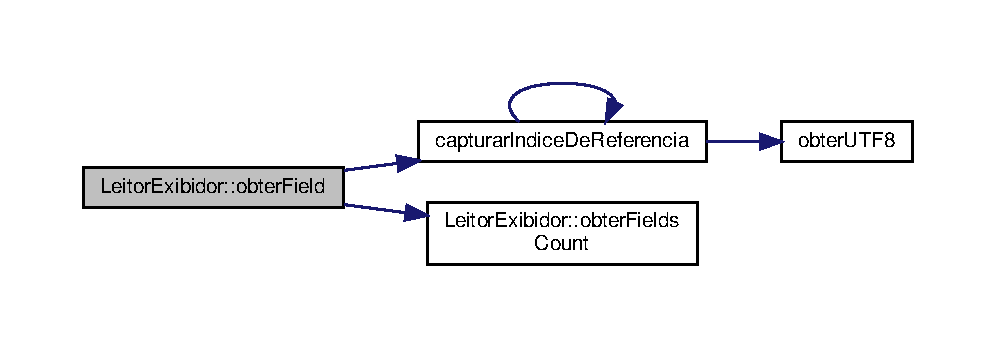
\includegraphics[width=350pt]{classLeitorExibidor_af51949669ace432f66221710ef3a3b00_cgraph}
\end{center}
\end{figure}
\mbox{\Hypertarget{classLeitorExibidor_a480bbed0d19b7cf5d64753c9c1210464}\label{classLeitorExibidor_a480bbed0d19b7cf5d64753c9c1210464}} 
\index{Leitor\+Exibidor@{Leitor\+Exibidor}!obter\+Fields@{obter\+Fields}}
\index{obter\+Fields@{obter\+Fields}!Leitor\+Exibidor@{Leitor\+Exibidor}}
\subsubsection{\texorpdfstring{obter\+Fields()}{obterFields()}}
{\footnotesize\ttfamily \hyperlink{structfield__info}{field\+\_\+info} Leitor\+Exibidor\+::obter\+Fields (\begin{DoxyParamCaption}{ }\end{DoxyParamCaption})}



Retorna a array com as fields lidas. 

\begin{DoxyReturn}{Retorna}
a array da struct \hyperlink{structfield__info}{field\+\_\+info} 
\end{DoxyReturn}


Definido na linha 500 do ficheiro Classe\+Leitor\+Exibidor.\+cpp.



Referências fields.



Referenciado por Instance\+Class\+::\+Instance\+Class() e Static\+Class\+::\+Static\+Class().

\mbox{\Hypertarget{classLeitorExibidor_a483e90f3d60c63a2b3d1106961c7f553}\label{classLeitorExibidor_a483e90f3d60c63a2b3d1106961c7f553}} 
\index{Leitor\+Exibidor@{Leitor\+Exibidor}!obter\+Fields\+Count@{obter\+Fields\+Count}}
\index{obter\+Fields\+Count@{obter\+Fields\+Count}!Leitor\+Exibidor@{Leitor\+Exibidor}}
\subsubsection{\texorpdfstring{obter\+Fields\+Count()}{obterFieldsCount()}}
{\footnotesize\ttfamily \hyperlink{BasicTypes_8h_a90240657108b1b457eef9d3f76e0202e}{U2} Leitor\+Exibidor\+::obter\+Fields\+Count (\begin{DoxyParamCaption}{ }\end{DoxyParamCaption})}



Retorna número de fields. 

\begin{DoxyReturn}{Retorna}
uint16\+\_\+t indicando o numero de fields 
\end{DoxyReturn}


Definido na linha 496 do ficheiro Classe\+Leitor\+Exibidor.\+cpp.



Referências fields\+Count.



Referenciado por Instance\+Class\+::\+Instance\+Class(), obter\+Field() e Static\+Class\+::\+Static\+Class().

\mbox{\Hypertarget{classLeitorExibidor_a161f1cc97c2c71c800cf588f8a4eab67}\label{classLeitorExibidor_a161f1cc97c2c71c800cf588f8a4eab67}} 
\index{Leitor\+Exibidor@{Leitor\+Exibidor}!obter\+Main@{obter\+Main}}
\index{obter\+Main@{obter\+Main}!Leitor\+Exibidor@{Leitor\+Exibidor}}
\subsubsection{\texorpdfstring{obter\+Main()}{obterMain()}}
{\footnotesize\ttfamily \hyperlink{structmethod__info}{method\+\_\+info} Leitor\+Exibidor\+::obter\+Main (\begin{DoxyParamCaption}{ }\end{DoxyParamCaption})}



Retorna o método main. 

\begin{DoxyReturn}{Retorna}
struct \hyperlink{structmethod__info}{method\+\_\+info} contendo informações sobre o método 
\end{DoxyReturn}


Definido na linha 350 do ficheiro Classe\+Leitor\+Exibidor.\+cpp.



Referências encontrou\+Main, main\+Method e methods.



Referenciado por Frame\+Stack\+::\+Frame\+Stack().

\mbox{\Hypertarget{classLeitorExibidor_a4d1a48fa9825d2cb2b520be79112408c}\label{classLeitorExibidor_a4d1a48fa9825d2cb2b520be79112408c}} 
\index{Leitor\+Exibidor@{Leitor\+Exibidor}!obter\+Method@{obter\+Method}}
\index{obter\+Method@{obter\+Method}!Leitor\+Exibidor@{Leitor\+Exibidor}}
\subsubsection{\texorpdfstring{obter\+Method()}{obterMethod()}}
{\footnotesize\ttfamily \hyperlink{structmethod__info}{method\+\_\+info} $\ast$ Leitor\+Exibidor\+::obter\+Method (\begin{DoxyParamCaption}\item[{string}]{nome,  }\item[{string}]{descriptor }\end{DoxyParamCaption})}


\begin{DoxyParams}{Parâmetros}
{\em nome} & Nome do method desejado \\
\hline
{\em descriptor} & Descritor do method desejado \\
\hline
\end{DoxyParams}


Definido na linha 515 do ficheiro Classe\+Leitor\+Exibidor.\+cpp.



Referências capturar\+Indice\+De\+Referencia(), constant\+Pool, method\+\_\+info\+::descriptor\+\_\+index, methods, methods\+Count, method\+\_\+info\+::name\+\_\+index, Method\+Area\+::obter\+Class(), Static\+Class\+::obter\+Classe\+Leitor\+Exibidor(), obter\+Method() e obter\+Super\+\_\+class().



Referenciado por Operations\+::invokeinterface(), Operations\+::invokespecial(), Operations\+::invokestatic(), Operations\+::invokevirtual() e obter\+Method().

Grafo de chamadas desta função\+:
\nopagebreak
\begin{figure}[H]
\begin{center}
\leavevmode
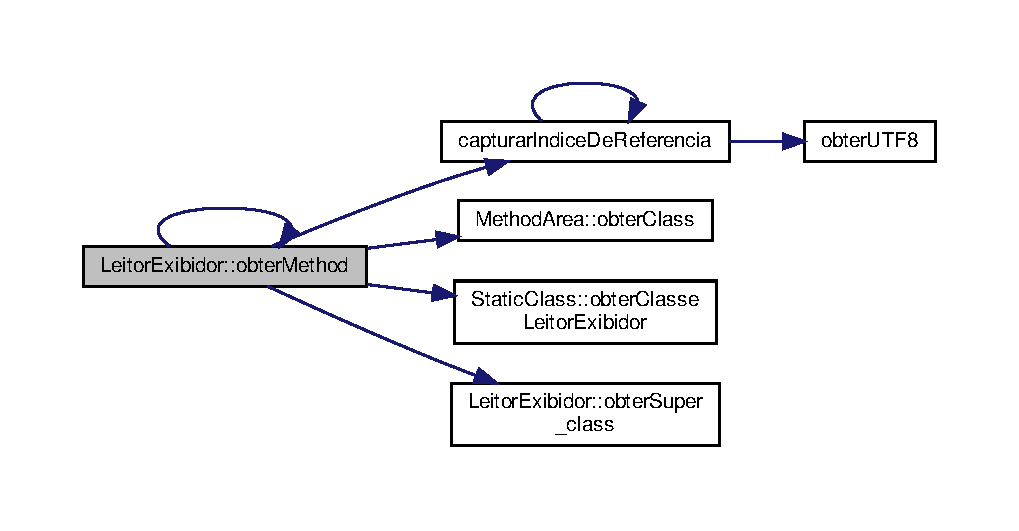
\includegraphics[width=350pt]{classLeitorExibidor_a4d1a48fa9825d2cb2b520be79112408c_cgraph}
\end{center}
\end{figure}
\mbox{\Hypertarget{classLeitorExibidor_a0fbc8db7d08d00ec8f12e26bbce93048}\label{classLeitorExibidor_a0fbc8db7d08d00ec8f12e26bbce93048}} 
\index{Leitor\+Exibidor@{Leitor\+Exibidor}!obter\+Methods@{obter\+Methods}}
\index{obter\+Methods@{obter\+Methods}!Leitor\+Exibidor@{Leitor\+Exibidor}}
\subsubsection{\texorpdfstring{obter\+Methods()}{obterMethods()}}
{\footnotesize\ttfamily \hyperlink{structmethod__info}{method\+\_\+info} $\ast$ Leitor\+Exibidor\+::obter\+Methods (\begin{DoxyParamCaption}{ }\end{DoxyParamCaption})}



Retorna todos os métodos. 

\begin{DoxyReturn}{Retorna}
array do tipo \hyperlink{structmethod__info}{method\+\_\+info} 
\end{DoxyReturn}


Definido na linha 480 do ficheiro Classe\+Leitor\+Exibidor.\+cpp.



Referências methods.

\mbox{\Hypertarget{classLeitorExibidor_aa9c91f4a145f4ef753c33f8898075930}\label{classLeitorExibidor_aa9c91f4a145f4ef753c33f8898075930}} 
\index{Leitor\+Exibidor@{Leitor\+Exibidor}!obter\+Methods\+Count@{obter\+Methods\+Count}}
\index{obter\+Methods\+Count@{obter\+Methods\+Count}!Leitor\+Exibidor@{Leitor\+Exibidor}}
\subsubsection{\texorpdfstring{obter\+Methods\+Count()}{obterMethodsCount()}}
{\footnotesize\ttfamily \hyperlink{BasicTypes_8h_a90240657108b1b457eef9d3f76e0202e}{U2} Leitor\+Exibidor\+::obter\+Methods\+Count (\begin{DoxyParamCaption}{ }\end{DoxyParamCaption})}



Retorna o numero de Methods. 

\begin{DoxyReturn}{Retorna}
uint16\+\_\+t indicando o numero de metodos 
\end{DoxyReturn}


Definido na linha 484 do ficheiro Classe\+Leitor\+Exibidor.\+cpp.



Referências methods\+Count.

\mbox{\Hypertarget{classLeitorExibidor_a74785a29369d04d5a7d14ed63a0b2102}\label{classLeitorExibidor_a74785a29369d04d5a7d14ed63a0b2102}} 
\index{Leitor\+Exibidor@{Leitor\+Exibidor}!obter\+Path@{obter\+Path}}
\index{obter\+Path@{obter\+Path}!Leitor\+Exibidor@{Leitor\+Exibidor}}
\subsubsection{\texorpdfstring{obter\+Path()}{obterPath()}}
{\footnotesize\ttfamily char $\ast$ Leitor\+Exibidor\+::obter\+Path (\begin{DoxyParamCaption}{ }\end{DoxyParamCaption})}



Pega o caminho do arquivo .class. 

\begin{DoxyReturn}{Retorna}
Retorna a string com o caminho total do arquivo 
\end{DoxyReturn}


Definido na linha 449 do ficheiro Classe\+Leitor\+Exibidor.\+cpp.



Referências file\+Name.



Referenciado por main().

\mbox{\Hypertarget{classLeitorExibidor_a6a9e55a1b824fed37f0841cb253789b2}\label{classLeitorExibidor_a6a9e55a1b824fed37f0841cb253789b2}} 
\index{Leitor\+Exibidor@{Leitor\+Exibidor}!obter\+Status@{obter\+Status}}
\index{obter\+Status@{obter\+Status}!Leitor\+Exibidor@{Leitor\+Exibidor}}
\subsubsection{\texorpdfstring{obter\+Status()}{obterStatus()}}
{\footnotesize\ttfamily int Leitor\+Exibidor\+::obter\+Status (\begin{DoxyParamCaption}{ }\end{DoxyParamCaption})}



Retorna o status lido, informando para o método que chamou o que aconteceu. 

\begin{DoxyReturn}{Retorna}
status 
\end{DoxyReturn}


Definido na linha 404 do ficheiro Classe\+Leitor\+Exibidor.\+cpp.



Referências status.



Referenciado por Method\+Area\+::adicionar\+Classe() e main().

\mbox{\Hypertarget{classLeitorExibidor_ab46841a0392f45a35a5444dca234a1ae}\label{classLeitorExibidor_ab46841a0392f45a35a5444dca234a1ae}} 
\index{Leitor\+Exibidor@{Leitor\+Exibidor}!obter\+Super\+\_\+class@{obter\+Super\+\_\+class}}
\index{obter\+Super\+\_\+class@{obter\+Super\+\_\+class}!Leitor\+Exibidor@{Leitor\+Exibidor}}
\subsubsection{\texorpdfstring{obter\+Super\+\_\+class()}{obterSuper\_class()}}
{\footnotesize\ttfamily \hyperlink{BasicTypes_8h_a90240657108b1b457eef9d3f76e0202e}{U2} Leitor\+Exibidor\+::obter\+Super\+\_\+class (\begin{DoxyParamCaption}{ }\end{DoxyParamCaption})}



Retorna um índice da constant pool que aponta para string com nome da superclass. 

\begin{DoxyReturn}{Retorna}
uint16\+\_\+t super\+\_\+class 
\end{DoxyReturn}


Definido na linha 492 do ficheiro Classe\+Leitor\+Exibidor.\+cpp.



Referências super\+\_\+class.



Referenciado por obter\+Class\+That\+Has\+Serached\+Method(), obter\+Method() e Operations\+::obter\+Static\+Class\+That\+Has\+Field().

\mbox{\Hypertarget{classLeitorExibidor_a7e64ad9d2b5f914f6bc4a0f84129f160}\label{classLeitorExibidor_a7e64ad9d2b5f914f6bc4a0f84129f160}} 
\index{Leitor\+Exibidor@{Leitor\+Exibidor}!obter\+Tamanho\+Constant\+Pool@{obter\+Tamanho\+Constant\+Pool}}
\index{obter\+Tamanho\+Constant\+Pool@{obter\+Tamanho\+Constant\+Pool}!Leitor\+Exibidor@{Leitor\+Exibidor}}
\subsubsection{\texorpdfstring{obter\+Tamanho\+Constant\+Pool()}{obterTamanhoConstantPool()}}
{\footnotesize\ttfamily \hyperlink{BasicTypes_8h_a90240657108b1b457eef9d3f76e0202e}{U2} Leitor\+Exibidor\+::obter\+Tamanho\+Constant\+Pool (\begin{DoxyParamCaption}{ }\end{DoxyParamCaption})}



Retorna o valor do tamanho da constant pool. 

\begin{DoxyReturn}{Retorna}
Retorna a array com a constant pool 
\end{DoxyReturn}


Definido na linha 445 do ficheiro Classe\+Leitor\+Exibidor.\+cpp.



Referências length\+CP.

\mbox{\Hypertarget{classLeitorExibidor_aa5cc18c3fb83811379d2f221980d8b8b}\label{classLeitorExibidor_aa5cc18c3fb83811379d2f221980d8b8b}} 
\index{Leitor\+Exibidor@{Leitor\+Exibidor}!obter\+This\+\_\+class@{obter\+This\+\_\+class}}
\index{obter\+This\+\_\+class@{obter\+This\+\_\+class}!Leitor\+Exibidor@{Leitor\+Exibidor}}
\subsubsection{\texorpdfstring{obter\+This\+\_\+class()}{obterThis\_class()}}
{\footnotesize\ttfamily \hyperlink{BasicTypes_8h_a90240657108b1b457eef9d3f76e0202e}{U2} Leitor\+Exibidor\+::obter\+This\+\_\+class (\begin{DoxyParamCaption}{ }\end{DoxyParamCaption})}



Retorna um índice da constant pool que aponta para string com nome da class. 

\begin{DoxyReturn}{Retorna}
uint16\+\_\+t this\+\_\+class 
\end{DoxyReturn}


Definido na linha 488 do ficheiro Classe\+Leitor\+Exibidor.\+cpp.



Referências this\+\_\+class.



Referenciado por Method\+Area\+::adicionar\+Classe().

\mbox{\Hypertarget{classLeitorExibidor_a422272b830079ee349b468bbe78d4b13}\label{classLeitorExibidor_a422272b830079ee349b468bbe78d4b13}} 
\index{Leitor\+Exibidor@{Leitor\+Exibidor}!validacao@{validacao}}
\index{validacao@{validacao}!Leitor\+Exibidor@{Leitor\+Exibidor}}
\subsubsection{\texorpdfstring{validacao()}{validacao()}}
{\footnotesize\ttfamily Leitor\+Exibidor\+::validacao (\begin{DoxyParamCaption}\item[{void}]{ }\end{DoxyParamCaption})}



Valida estrutura obrigatoria. 



Definido na linha 45 do ficheiro Classe\+Leitor\+Exibidor.\+cpp.



Referências I\+N\+V\+A\+L\+I\+D\+\_\+\+E\+X\+T\+E\+N\+S\+I\+ON, I\+N\+V\+A\+L\+I\+D\+\_\+\+N\+A\+ME, M\+I\+S\+S\+I\+N\+G\+\_\+\+M\+A\+IN, obter\+Erro(), status, validar\+Extensao(), verificar\+Main() e verificar\+This\+Class().



Referenciado por main().

Grafo de chamadas desta função\+:
\nopagebreak
\begin{figure}[H]
\begin{center}
\leavevmode
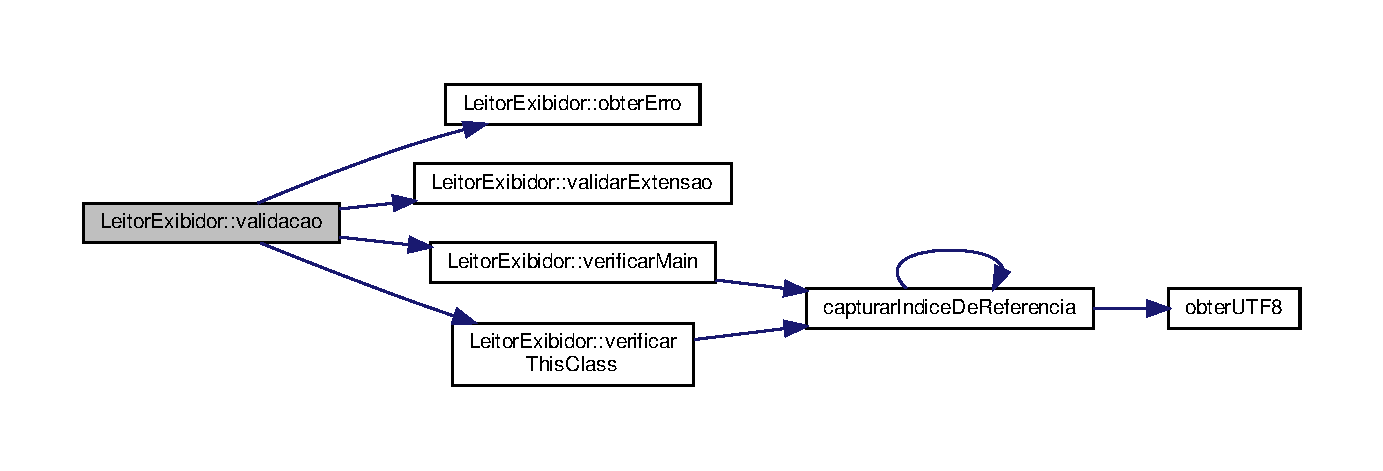
\includegraphics[width=350pt]{classLeitorExibidor_a422272b830079ee349b468bbe78d4b13_cgraph}
\end{center}
\end{figure}
\mbox{\Hypertarget{classLeitorExibidor_a83ed9ca5a7b4442ae3449daffc0d3d5c}\label{classLeitorExibidor_a83ed9ca5a7b4442ae3449daffc0d3d5c}} 
\index{Leitor\+Exibidor@{Leitor\+Exibidor}!validar\+Extensao@{validar\+Extensao}}
\index{validar\+Extensao@{validar\+Extensao}!Leitor\+Exibidor@{Leitor\+Exibidor}}
\subsubsection{\texorpdfstring{validar\+Extensao()}{validarExtensao()}}
{\footnotesize\ttfamily bool Leitor\+Exibidor\+::validar\+Extensao (\begin{DoxyParamCaption}{ }\end{DoxyParamCaption})}



Verifica se a extensão do arquivo é .class. 

\begin{DoxyReturn}{Retorna}
booleano que indica se existe o .class 
\end{DoxyReturn}


Definido na linha 284 do ficheiro Classe\+Leitor\+Exibidor.\+cpp.



Referências file\+Name.



Referenciado por Method\+Area\+::adicionar\+Classe(), carregar() e validacao().

\mbox{\Hypertarget{classLeitorExibidor_a8aeff3d072e77288215e5a070e958cf0}\label{classLeitorExibidor_a8aeff3d072e77288215e5a070e958cf0}} 
\index{Leitor\+Exibidor@{Leitor\+Exibidor}!verificar\+Clinit@{verificar\+Clinit}}
\index{verificar\+Clinit@{verificar\+Clinit}!Leitor\+Exibidor@{Leitor\+Exibidor}}
\subsubsection{\texorpdfstring{verificar\+Clinit()}{verificarClinit()}}
{\footnotesize\ttfamily bool Leitor\+Exibidor\+::verificar\+Clinit (\begin{DoxyParamCaption}{ }\end{DoxyParamCaption})\hspace{0.3cm}{\ttfamily [private]}}



Encontra em qual method esta a clinit, se existir. 

\begin{DoxyReturn}{Retorna}
booleano que indica se existe o metodo clinit 
\end{DoxyReturn}


Definido na linha 320 do ficheiro Classe\+Leitor\+Exibidor.\+cpp.



Referências capturar\+Indice\+De\+Referencia(), clinit, constant\+Pool, methods, methods\+Count e method\+\_\+info\+::name\+\_\+index.



Referenciado por carregar() e existe\+Clinit().

Grafo de chamadas desta função\+:
\nopagebreak
\begin{figure}[H]
\begin{center}
\leavevmode
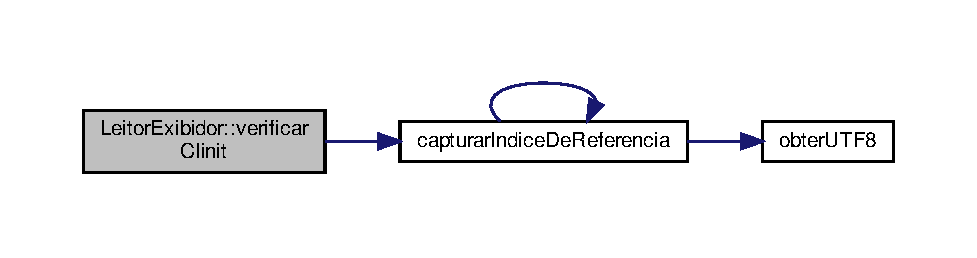
\includegraphics[width=350pt]{classLeitorExibidor_a8aeff3d072e77288215e5a070e958cf0_cgraph}
\end{center}
\end{figure}
\mbox{\Hypertarget{classLeitorExibidor_a2d486c9289a5d50a7fb00afffd2fa760}\label{classLeitorExibidor_a2d486c9289a5d50a7fb00afffd2fa760}} 
\index{Leitor\+Exibidor@{Leitor\+Exibidor}!verificar\+Main@{verificar\+Main}}
\index{verificar\+Main@{verificar\+Main}!Leitor\+Exibidor@{Leitor\+Exibidor}}
\subsubsection{\texorpdfstring{verificar\+Main()}{verificarMain()}}
{\footnotesize\ttfamily bool Leitor\+Exibidor\+::verificar\+Main (\begin{DoxyParamCaption}{ }\end{DoxyParamCaption})\hspace{0.3cm}{\ttfamily [private]}}



Encontro em qual method está a main. 

\begin{DoxyReturn}{Retorna}
booleano que indica se existe o metodo main 
\end{DoxyReturn}


Definido na linha 297 do ficheiro Classe\+Leitor\+Exibidor.\+cpp.



Referências method\+\_\+info\+::access\+\_\+flags, capturar\+Indice\+De\+Referencia(), constant\+Pool, method\+\_\+info\+::descriptor\+\_\+index, main\+Method, methods, methods\+Count e method\+\_\+info\+::name\+\_\+index.



Referenciado por carregar(), existe\+Main() e validacao().

Grafo de chamadas desta função\+:
\nopagebreak
\begin{figure}[H]
\begin{center}
\leavevmode
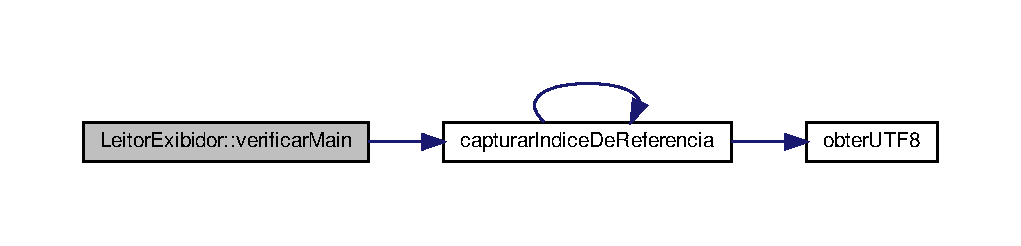
\includegraphics[width=350pt]{classLeitorExibidor_a2d486c9289a5d50a7fb00afffd2fa760_cgraph}
\end{center}
\end{figure}
\mbox{\Hypertarget{classLeitorExibidor_a89d56b461514ed8fea8987ee52fa2eb9}\label{classLeitorExibidor_a89d56b461514ed8fea8987ee52fa2eb9}} 
\index{Leitor\+Exibidor@{Leitor\+Exibidor}!verificar\+This\+Class@{verificar\+This\+Class}}
\index{verificar\+This\+Class@{verificar\+This\+Class}!Leitor\+Exibidor@{Leitor\+Exibidor}}
\subsubsection{\texorpdfstring{verificar\+This\+Class()}{verificarThisClass()}}
{\footnotesize\ttfamily bool Leitor\+Exibidor\+::verificar\+This\+Class (\begin{DoxyParamCaption}{ }\end{DoxyParamCaption})}



Verifica se a class definida é igual ao nome da classe sem extensões. 

\begin{DoxyReturn}{Retorna}
booleano indicando se a .class está correta 
\end{DoxyReturn}


Definido na linha 362 do ficheiro Classe\+Leitor\+Exibidor.\+cpp.



Referências capturar\+Indice\+De\+Referencia(), constant\+Pool, file\+Name e this\+\_\+class.



Referenciado por carregar() e validacao().

Grafo de chamadas desta função\+:
\nopagebreak
\begin{figure}[H]
\begin{center}
\leavevmode
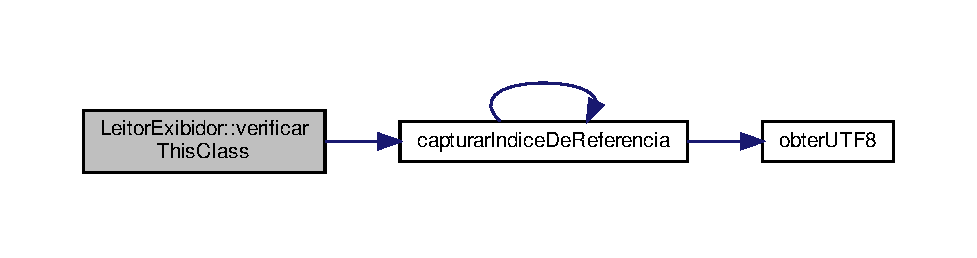
\includegraphics[width=350pt]{classLeitorExibidor_a89d56b461514ed8fea8987ee52fa2eb9_cgraph}
\end{center}
\end{figure}


\subsection{Documentação dos dados membro}
\mbox{\Hypertarget{classLeitorExibidor_a16d6ecbc6b367cda3c0b774505285665}\label{classLeitorExibidor_a16d6ecbc6b367cda3c0b774505285665}} 
\index{Leitor\+Exibidor@{Leitor\+Exibidor}!access\+Flags@{access\+Flags}}
\index{access\+Flags@{access\+Flags}!Leitor\+Exibidor@{Leitor\+Exibidor}}
\subsubsection{\texorpdfstring{access\+Flags}{accessFlags}}
{\footnotesize\ttfamily \hyperlink{BasicTypes_8h_a90240657108b1b457eef9d3f76e0202e}{U2} Leitor\+Exibidor\+::access\+Flags\hspace{0.3cm}{\ttfamily [private]}}



Definido na linha 248 do ficheiro Classe\+Leitor\+Exibidor.\+h.



Referenciado por carregar(), gravar\+Arquivo\+Informacoes\+Gerais() e imprimir\+Informacoes\+Gerais().

\mbox{\Hypertarget{classLeitorExibidor_acbb3d188113d55cc00b6e92bf2fddb98}\label{classLeitorExibidor_acbb3d188113d55cc00b6e92bf2fddb98}} 
\index{Leitor\+Exibidor@{Leitor\+Exibidor}!arquivo\+Class@{arquivo\+Class}}
\index{arquivo\+Class@{arquivo\+Class}!Leitor\+Exibidor@{Leitor\+Exibidor}}
\subsubsection{\texorpdfstring{arquivo\+Class}{arquivoClass}}
{\footnotesize\ttfamily F\+I\+LE$\ast$ Leitor\+Exibidor\+::arquivo\+Class\hspace{0.3cm}{\ttfamily [private]}}



Definido na linha 254 do ficheiro Classe\+Leitor\+Exibidor.\+h.



Referenciado por carregar().

\mbox{\Hypertarget{classLeitorExibidor_ae7f2edb9968df63470901712119e30d2}\label{classLeitorExibidor_ae7f2edb9968df63470901712119e30d2}} 
\index{Leitor\+Exibidor@{Leitor\+Exibidor}!arquivo\+Saida@{arquivo\+Saida}}
\index{arquivo\+Saida@{arquivo\+Saida}!Leitor\+Exibidor@{Leitor\+Exibidor}}
\subsubsection{\texorpdfstring{arquivo\+Saida}{arquivoSaida}}
{\footnotesize\ttfamily fstream Leitor\+Exibidor\+::arquivo\+Saida\hspace{0.3cm}{\ttfamily [private]}}



Definido na linha 255 do ficheiro Classe\+Leitor\+Exibidor.\+h.



Referenciado por fechar\+Arquivo(), gravar\+Arquivo(), gravar\+Arquivo\+Informacoes\+Gerais() e inicializar\+Arquivo().

\mbox{\Hypertarget{classLeitorExibidor_adb26d0959bef738b08bffa009d12fac3}\label{classLeitorExibidor_adb26d0959bef738b08bffa009d12fac3}} 
\index{Leitor\+Exibidor@{Leitor\+Exibidor}!attributes@{attributes}}
\index{attributes@{attributes}!Leitor\+Exibidor@{Leitor\+Exibidor}}
\subsubsection{\texorpdfstring{attributes}{attributes}}
{\footnotesize\ttfamily \hyperlink{structattribute__info}{attribute\+\_\+info}$\ast$ Leitor\+Exibidor\+::attributes\hspace{0.3cm}{\ttfamily [private]}}



Definido na linha 253 do ficheiro Classe\+Leitor\+Exibidor.\+h.



Referenciado por carregar(), exibir() e gravar\+Arquivo().

\mbox{\Hypertarget{classLeitorExibidor_ac42b42a9a6c94c260db0016df94cda1d}\label{classLeitorExibidor_ac42b42a9a6c94c260db0016df94cda1d}} 
\index{Leitor\+Exibidor@{Leitor\+Exibidor}!attributes\+Count@{attributes\+Count}}
\index{attributes\+Count@{attributes\+Count}!Leitor\+Exibidor@{Leitor\+Exibidor}}
\subsubsection{\texorpdfstring{attributes\+Count}{attributesCount}}
{\footnotesize\ttfamily \hyperlink{BasicTypes_8h_a90240657108b1b457eef9d3f76e0202e}{U2} Leitor\+Exibidor\+::attributes\+Count\hspace{0.3cm}{\ttfamily [private]}}



Definido na linha 248 do ficheiro Classe\+Leitor\+Exibidor.\+h.



Referenciado por carregar(), exibir(), gravar\+Arquivo(), gravar\+Arquivo\+Informacoes\+Gerais() e imprimir\+Informacoes\+Gerais().

\mbox{\Hypertarget{classLeitorExibidor_a0c4c896a1baf647a282881524f8a9687}\label{classLeitorExibidor_a0c4c896a1baf647a282881524f8a9687}} 
\index{Leitor\+Exibidor@{Leitor\+Exibidor}!clinit@{clinit}}
\index{clinit@{clinit}!Leitor\+Exibidor@{Leitor\+Exibidor}}
\subsubsection{\texorpdfstring{clinit}{clinit}}
{\footnotesize\ttfamily int Leitor\+Exibidor\+::clinit\hspace{0.3cm}{\ttfamily [private]}}



Definido na linha 243 do ficheiro Classe\+Leitor\+Exibidor.\+h.



Referenciado por obter\+Clinit() e verificar\+Clinit().

\mbox{\Hypertarget{classLeitorExibidor_ac92916cbf475e31ce0f2475d982ddaea}\label{classLeitorExibidor_ac92916cbf475e31ce0f2475d982ddaea}} 
\index{Leitor\+Exibidor@{Leitor\+Exibidor}!constant\+Pool@{constant\+Pool}}
\index{constant\+Pool@{constant\+Pool}!Leitor\+Exibidor@{Leitor\+Exibidor}}
\subsubsection{\texorpdfstring{constant\+Pool}{constantPool}}
{\footnotesize\ttfamily \hyperlink{structcp__info}{cp\+\_\+info}$\ast$ Leitor\+Exibidor\+::constant\+Pool\hspace{0.3cm}{\ttfamily [private]}}



Definido na linha 250 do ficheiro Classe\+Leitor\+Exibidor.\+h.



Referenciado por carregar(), exibir(), gravar\+Arquivo(), gravar\+Arquivo\+Informacoes\+Gerais(), imprimir\+Informacoes\+Gerais(), obter\+Class\+That\+Has\+Serached\+Method(), obter\+Constant\+Pool(), obter\+Field(), obter\+Method(), verificar\+Clinit(), verificar\+Main() e verificar\+This\+Class().

\mbox{\Hypertarget{classLeitorExibidor_a93a1aa14204f0445a97304cc504a3cf0}\label{classLeitorExibidor_a93a1aa14204f0445a97304cc504a3cf0}} 
\index{Leitor\+Exibidor@{Leitor\+Exibidor}!encontrou\+Clinit@{encontrou\+Clinit}}
\index{encontrou\+Clinit@{encontrou\+Clinit}!Leitor\+Exibidor@{Leitor\+Exibidor}}
\subsubsection{\texorpdfstring{encontrou\+Clinit}{encontrouClinit}}
{\footnotesize\ttfamily bool Leitor\+Exibidor\+::encontrou\+Clinit\hspace{0.3cm}{\ttfamily [private]}}



Definido na linha 244 do ficheiro Classe\+Leitor\+Exibidor.\+h.



Referenciado por carregar() e existe\+Clinit().

\mbox{\Hypertarget{classLeitorExibidor_aca32f682d0ccd1d60a76d0833ca0617f}\label{classLeitorExibidor_aca32f682d0ccd1d60a76d0833ca0617f}} 
\index{Leitor\+Exibidor@{Leitor\+Exibidor}!encontrou\+Main@{encontrou\+Main}}
\index{encontrou\+Main@{encontrou\+Main}!Leitor\+Exibidor@{Leitor\+Exibidor}}
\subsubsection{\texorpdfstring{encontrou\+Main}{encontrouMain}}
{\footnotesize\ttfamily bool Leitor\+Exibidor\+::encontrou\+Main\hspace{0.3cm}{\ttfamily [private]}}



Definido na linha 244 do ficheiro Classe\+Leitor\+Exibidor.\+h.



Referenciado por carregar(), existe\+Main() e obter\+Main().

\mbox{\Hypertarget{classLeitorExibidor_a6e8475e2db54d776db636c06d823eb3f}\label{classLeitorExibidor_a6e8475e2db54d776db636c06d823eb3f}} 
\index{Leitor\+Exibidor@{Leitor\+Exibidor}!fields@{fields}}
\index{fields@{fields}!Leitor\+Exibidor@{Leitor\+Exibidor}}
\subsubsection{\texorpdfstring{fields}{fields}}
{\footnotesize\ttfamily \hyperlink{structfield__info}{field\+\_\+info}$\ast$ Leitor\+Exibidor\+::fields\hspace{0.3cm}{\ttfamily [private]}}



Definido na linha 251 do ficheiro Classe\+Leitor\+Exibidor.\+h.



Referenciado por carregar(), exibir(), gravar\+Arquivo(), obter\+Field() e obter\+Fields().

\mbox{\Hypertarget{classLeitorExibidor_a9a54627d53b9a3c25c5ba71977e1e002}\label{classLeitorExibidor_a9a54627d53b9a3c25c5ba71977e1e002}} 
\index{Leitor\+Exibidor@{Leitor\+Exibidor}!fields\+Count@{fields\+Count}}
\index{fields\+Count@{fields\+Count}!Leitor\+Exibidor@{Leitor\+Exibidor}}
\subsubsection{\texorpdfstring{fields\+Count}{fieldsCount}}
{\footnotesize\ttfamily \hyperlink{BasicTypes_8h_a90240657108b1b457eef9d3f76e0202e}{U2} Leitor\+Exibidor\+::fields\+Count\hspace{0.3cm}{\ttfamily [private]}}



Definido na linha 247 do ficheiro Classe\+Leitor\+Exibidor.\+h.



Referenciado por carregar(), exibir(), gravar\+Arquivo(), gravar\+Arquivo\+Informacoes\+Gerais(), imprimir\+Informacoes\+Gerais() e obter\+Fields\+Count().

\mbox{\Hypertarget{classLeitorExibidor_a1dfa84388856ad4d83883e4e5548b485}\label{classLeitorExibidor_a1dfa84388856ad4d83883e4e5548b485}} 
\index{Leitor\+Exibidor@{Leitor\+Exibidor}!file\+Name@{file\+Name}}
\index{file\+Name@{file\+Name}!Leitor\+Exibidor@{Leitor\+Exibidor}}
\subsubsection{\texorpdfstring{file\+Name}{fileName}}
{\footnotesize\ttfamily char$\ast$ Leitor\+Exibidor\+::file\+Name\hspace{0.3cm}{\ttfamily [private]}}



Definido na linha 245 do ficheiro Classe\+Leitor\+Exibidor.\+h.



Referenciado por carregar(), Leitor\+Exibidor(), obter\+Erro(), obter\+Path(), validar\+Extensao() e verificar\+This\+Class().

\mbox{\Hypertarget{classLeitorExibidor_a7c19cc595c9d806b30477b5b008f3caa}\label{classLeitorExibidor_a7c19cc595c9d806b30477b5b008f3caa}} 
\index{Leitor\+Exibidor@{Leitor\+Exibidor}!interfaces@{interfaces}}
\index{interfaces@{interfaces}!Leitor\+Exibidor@{Leitor\+Exibidor}}
\subsubsection{\texorpdfstring{interfaces}{interfaces}}
{\footnotesize\ttfamily \hyperlink{BasicTypes_8h_a90240657108b1b457eef9d3f76e0202e}{U2}$\ast$ Leitor\+Exibidor\+::interfaces\hspace{0.3cm}{\ttfamily [private]}}



Definido na linha 249 do ficheiro Classe\+Leitor\+Exibidor.\+h.



Referenciado por carregar(), exibir() e gravar\+Arquivo().

\mbox{\Hypertarget{classLeitorExibidor_a596a1440982d2418e39adf5b1857ab15}\label{classLeitorExibidor_a596a1440982d2418e39adf5b1857ab15}} 
\index{Leitor\+Exibidor@{Leitor\+Exibidor}!interfaces\+Count@{interfaces\+Count}}
\index{interfaces\+Count@{interfaces\+Count}!Leitor\+Exibidor@{Leitor\+Exibidor}}
\subsubsection{\texorpdfstring{interfaces\+Count}{interfacesCount}}
{\footnotesize\ttfamily \hyperlink{BasicTypes_8h_a90240657108b1b457eef9d3f76e0202e}{U2} Leitor\+Exibidor\+::interfaces\+Count\hspace{0.3cm}{\ttfamily [private]}}



Definido na linha 247 do ficheiro Classe\+Leitor\+Exibidor.\+h.



Referenciado por carregar(), exibir(), gravar\+Arquivo(), gravar\+Arquivo\+Informacoes\+Gerais() e imprimir\+Informacoes\+Gerais().

\mbox{\Hypertarget{classLeitorExibidor_ae891dce6b86c2d09c1a112bd585561d6}\label{classLeitorExibidor_ae891dce6b86c2d09c1a112bd585561d6}} 
\index{Leitor\+Exibidor@{Leitor\+Exibidor}!length\+CP@{length\+CP}}
\index{length\+CP@{length\+CP}!Leitor\+Exibidor@{Leitor\+Exibidor}}
\subsubsection{\texorpdfstring{length\+CP}{lengthCP}}
{\footnotesize\ttfamily \hyperlink{BasicTypes_8h_a90240657108b1b457eef9d3f76e0202e}{U2} Leitor\+Exibidor\+::length\+CP\hspace{0.3cm}{\ttfamily [private]}}



Definido na linha 246 do ficheiro Classe\+Leitor\+Exibidor.\+h.



Referenciado por carregar(), exibir(), gravar\+Arquivo(), gravar\+Arquivo\+Informacoes\+Gerais(), imprimir\+Informacoes\+Gerais() e obter\+Tamanho\+Constant\+Pool().

\mbox{\Hypertarget{classLeitorExibidor_a9e7a108ebca3fac0096fcb422f2393db}\label{classLeitorExibidor_a9e7a108ebca3fac0096fcb422f2393db}} 
\index{Leitor\+Exibidor@{Leitor\+Exibidor}!main\+Method@{main\+Method}}
\index{main\+Method@{main\+Method}!Leitor\+Exibidor@{Leitor\+Exibidor}}
\subsubsection{\texorpdfstring{main\+Method}{mainMethod}}
{\footnotesize\ttfamily int Leitor\+Exibidor\+::main\+Method\hspace{0.3cm}{\ttfamily [private]}}



Definido na linha 243 do ficheiro Classe\+Leitor\+Exibidor.\+h.



Referenciado por obter\+Main() e verificar\+Main().

\mbox{\Hypertarget{classLeitorExibidor_a5c2cd58569e9c3fdc47c0bbab116b870}\label{classLeitorExibidor_a5c2cd58569e9c3fdc47c0bbab116b870}} 
\index{Leitor\+Exibidor@{Leitor\+Exibidor}!maj\+Version@{maj\+Version}}
\index{maj\+Version@{maj\+Version}!Leitor\+Exibidor@{Leitor\+Exibidor}}
\subsubsection{\texorpdfstring{maj\+Version}{majVersion}}
{\footnotesize\ttfamily \hyperlink{BasicTypes_8h_a90240657108b1b457eef9d3f76e0202e}{U2} Leitor\+Exibidor\+::maj\+Version\hspace{0.3cm}{\ttfamily [private]}}



Definido na linha 246 do ficheiro Classe\+Leitor\+Exibidor.\+h.



Referenciado por carregar(), gravar\+Arquivo\+Informacoes\+Gerais() e imprimir\+Informacoes\+Gerais().

\mbox{\Hypertarget{classLeitorExibidor_a0c9110ffe495c55bedaafdc47656eaed}\label{classLeitorExibidor_a0c9110ffe495c55bedaafdc47656eaed}} 
\index{Leitor\+Exibidor@{Leitor\+Exibidor}!methods@{methods}}
\index{methods@{methods}!Leitor\+Exibidor@{Leitor\+Exibidor}}
\subsubsection{\texorpdfstring{methods}{methods}}
{\footnotesize\ttfamily \hyperlink{structmethod__info}{method\+\_\+info}$\ast$ Leitor\+Exibidor\+::methods\hspace{0.3cm}{\ttfamily [private]}}



Definido na linha 252 do ficheiro Classe\+Leitor\+Exibidor.\+h.



Referenciado por carregar(), exibir(), gravar\+Arquivo(), obter\+Class\+That\+Has\+Serached\+Method(), obter\+Clinit(), obter\+Main(), obter\+Method(), obter\+Methods(), verificar\+Clinit() e verificar\+Main().

\mbox{\Hypertarget{classLeitorExibidor_a3f5d59fb172e478ab6d1a595a8b6c54a}\label{classLeitorExibidor_a3f5d59fb172e478ab6d1a595a8b6c54a}} 
\index{Leitor\+Exibidor@{Leitor\+Exibidor}!methods\+Count@{methods\+Count}}
\index{methods\+Count@{methods\+Count}!Leitor\+Exibidor@{Leitor\+Exibidor}}
\subsubsection{\texorpdfstring{methods\+Count}{methodsCount}}
{\footnotesize\ttfamily \hyperlink{BasicTypes_8h_a90240657108b1b457eef9d3f76e0202e}{U2} Leitor\+Exibidor\+::methods\+Count\hspace{0.3cm}{\ttfamily [private]}}



Definido na linha 248 do ficheiro Classe\+Leitor\+Exibidor.\+h.



Referenciado por carregar(), exibir(), gravar\+Arquivo(), gravar\+Arquivo\+Informacoes\+Gerais(), imprimir\+Informacoes\+Gerais(), obter\+Class\+That\+Has\+Serached\+Method(), obter\+Method(), obter\+Methods\+Count(), verificar\+Clinit() e verificar\+Main().

\mbox{\Hypertarget{classLeitorExibidor_a6f6ac6ed85979359308c07c666316218}\label{classLeitorExibidor_a6f6ac6ed85979359308c07c666316218}} 
\index{Leitor\+Exibidor@{Leitor\+Exibidor}!min\+Version@{min\+Version}}
\index{min\+Version@{min\+Version}!Leitor\+Exibidor@{Leitor\+Exibidor}}
\subsubsection{\texorpdfstring{min\+Version}{minVersion}}
{\footnotesize\ttfamily \hyperlink{BasicTypes_8h_a90240657108b1b457eef9d3f76e0202e}{U2} Leitor\+Exibidor\+::min\+Version\hspace{0.3cm}{\ttfamily [private]}}



Definido na linha 246 do ficheiro Classe\+Leitor\+Exibidor.\+h.



Referenciado por carregar(), gravar\+Arquivo\+Informacoes\+Gerais() e imprimir\+Informacoes\+Gerais().

\mbox{\Hypertarget{classLeitorExibidor_ac54b88860544d66f5e8f620c4c017a37}\label{classLeitorExibidor_ac54b88860544d66f5e8f620c4c017a37}} 
\index{Leitor\+Exibidor@{Leitor\+Exibidor}!status@{status}}
\index{status@{status}!Leitor\+Exibidor@{Leitor\+Exibidor}}
\subsubsection{\texorpdfstring{status}{status}}
{\footnotesize\ttfamily int Leitor\+Exibidor\+::status\hspace{0.3cm}{\ttfamily [private]}}



Definido na linha 243 do ficheiro Classe\+Leitor\+Exibidor.\+h.



Referenciado por carregar(), exibir(), gravar\+Arquivo(), inicializar\+Arquivo(), Leitor\+Exibidor(), obter\+Status() e validacao().

\mbox{\Hypertarget{classLeitorExibidor_adc9f3b119883f9bc4ba0323b8480c53e}\label{classLeitorExibidor_adc9f3b119883f9bc4ba0323b8480c53e}} 
\index{Leitor\+Exibidor@{Leitor\+Exibidor}!super\+\_\+class@{super\+\_\+class}}
\index{super\+\_\+class@{super\+\_\+class}!Leitor\+Exibidor@{Leitor\+Exibidor}}
\subsubsection{\texorpdfstring{super\+\_\+class}{super\_class}}
{\footnotesize\ttfamily \hyperlink{BasicTypes_8h_a90240657108b1b457eef9d3f76e0202e}{U2} Leitor\+Exibidor\+::super\+\_\+class\hspace{0.3cm}{\ttfamily [private]}}



Definido na linha 247 do ficheiro Classe\+Leitor\+Exibidor.\+h.



Referenciado por carregar(), gravar\+Arquivo\+Informacoes\+Gerais(), imprimir\+Informacoes\+Gerais() e obter\+Super\+\_\+class().

\mbox{\Hypertarget{classLeitorExibidor_ad85a876f6368ae8101343f4f35b53019}\label{classLeitorExibidor_ad85a876f6368ae8101343f4f35b53019}} 
\index{Leitor\+Exibidor@{Leitor\+Exibidor}!this\+\_\+class@{this\+\_\+class}}
\index{this\+\_\+class@{this\+\_\+class}!Leitor\+Exibidor@{Leitor\+Exibidor}}
\subsubsection{\texorpdfstring{this\+\_\+class}{this\_class}}
{\footnotesize\ttfamily \hyperlink{BasicTypes_8h_a90240657108b1b457eef9d3f76e0202e}{U2} Leitor\+Exibidor\+::this\+\_\+class\hspace{0.3cm}{\ttfamily [private]}}



Definido na linha 247 do ficheiro Classe\+Leitor\+Exibidor.\+h.



Referenciado por carregar(), gravar\+Arquivo\+Informacoes\+Gerais(), imprimir\+Informacoes\+Gerais(), obter\+This\+\_\+class() e verificar\+This\+Class().



A documentação para esta classe foi gerada a partir dos seguintes ficheiros\+:\begin{DoxyCompactItemize}
\item 
include/\hyperlink{ClasseLeitorExibidor_8h}{Classe\+Leitor\+Exibidor.\+h}\item 
src/\hyperlink{ClasseLeitorExibidor_8cpp}{Classe\+Leitor\+Exibidor.\+cpp}\end{DoxyCompactItemize}

\hypertarget{classLocalVariables}{}\section{Referência à classe Local\+Variables}
\label{classLocalVariables}\index{Local\+Variables@{Local\+Variables}}


{\ttfamily \#include $<$Local\+Variables.\+h$>$}

\subsection*{Membros públicos}
\begin{DoxyCompactItemize}
\item 
\hyperlink{classLocalVariables_ae354d02f996f4f584fe857d9304161c1}{Local\+Variables} (uint16\+\_\+t)
\begin{DoxyCompactList}\small\item\em \hyperlink{classVariaveisLocais}{Variaveis\+Locais} class constructor. \end{DoxyCompactList}\item 
\hyperlink{classLocalVariables_a2c9e8aefc8aa8ff0d0efd305ab3e424b}{Local\+Variables} (uint16\+\_\+t max\+Size, bool slots)
\begin{DoxyCompactList}\small\item\em \hyperlink{classLocalVariables}{Local\+Variables} class constructor. \end{DoxyCompactList}\item 
\hyperlink{classLocalVariables_aaf00f6cc3391fdd2cc0ecd2b1d31c887}{$\sim$\+Local\+Variables} ()
\begin{DoxyCompactList}\small\item\em Destructor 4. \end{DoxyCompactList}\item 
void \hyperlink{classLocalVariables_a6f51e8532ae59a4eea6801872d5f8444}{imprimir\+All} () const
\begin{DoxyCompactList}\small\item\em Function to show all values. \end{DoxyCompactList}\item 
void \hyperlink{classLocalVariables_a6d79e0c874931e97ed68a25cf60ab119}{set} (int, \hyperlink{BasicTypes_8h_a97b332303b1262282599e6ede0637b82}{Typed\+Element})
\begin{DoxyCompactList}\small\item\em Receives the typed element and inserts on past index. \end{DoxyCompactList}\item 
\hyperlink{BasicTypes_8h_a97b332303b1262282599e6ede0637b82}{Typed\+Element} \hyperlink{classLocalVariables_a4abbb4a732d7dd0f11a147b79c15ae10}{get} (int) const
\begin{DoxyCompactList}\small\item\em Gets element on past position by index. \end{DoxyCompactList}\item 
int \hyperlink{classLocalVariables_acf8ee1db2a3427c30eb3e489d7a4478c}{obter\+Max} () const
\begin{DoxyCompactList}\small\item\em Function to know maximum size. \end{DoxyCompactList}\item 
const \hyperlink{BasicTypes_8h_a97b332303b1262282599e6ede0637b82}{Typed\+Element} \hyperlink{classLocalVariables_a6e978f3c992385f2909261e995105142}{operator\mbox{[}$\,$\mbox{]}} (const int) const
\begin{DoxyCompactList}\small\item\em Function to allow class use like a struct\textquotesingle{}s array. \end{DoxyCompactList}\end{DoxyCompactItemize}
\subsection*{Atributos Privados}
\begin{DoxyCompactItemize}
\item 
uint32\+\_\+t $\ast$ \hyperlink{classLocalVariables_a0015e9d8a61d4643f6f3594785467ae4}{elements}
\item 
uint8\+\_\+t $\ast$ \hyperlink{classLocalVariables_ac73d4583cc3f8b295c8c986cee21fe30}{types}
\item 
const uint16\+\_\+t \hyperlink{classLocalVariables_a55f33aaf9a0af5176d460616402c4aeb}{max}
\item 
const uint16\+\_\+t \hyperlink{classLocalVariables_a892e685ce3c1c5e6da9e1db542d865e9}{real\+Max}
\item 
const bool \hyperlink{classLocalVariables_a8357edb6ae793a8f031ae3733751e1fc}{dois}
\end{DoxyCompactItemize}


\subsection{Descrição detalhada}


Definido na linha 36 do ficheiro Local\+Variables.\+h.



\subsection{Documentação dos Construtores \& Destrutor}
\mbox{\Hypertarget{classLocalVariables_ae354d02f996f4f584fe857d9304161c1}\label{classLocalVariables_ae354d02f996f4f584fe857d9304161c1}} 
\index{Local\+Variables@{Local\+Variables}!Local\+Variables@{Local\+Variables}}
\index{Local\+Variables@{Local\+Variables}!Local\+Variables@{Local\+Variables}}
\subsubsection{\texorpdfstring{Local\+Variables()}{LocalVariables()}\hspace{0.1cm}{\footnotesize\ttfamily [1/2]}}
{\footnotesize\ttfamily Local\+Variables\+::\+Local\+Variables (\begin{DoxyParamCaption}\item[{uint16\+\_\+t}]{max\+Size }\end{DoxyParamCaption})}



\hyperlink{classVariaveisLocais}{Variaveis\+Locais} class constructor. 


\begin{DoxyParams}{Parâmetros}
{\em max\+Size} & Maximum size of local variables that can be stored \\
\hline
\end{DoxyParams}


Definido na linha 8 do ficheiro Local\+Variables.\+cpp.



Referências elements, max e types.

\mbox{\Hypertarget{classLocalVariables_a2c9e8aefc8aa8ff0d0efd305ab3e424b}\label{classLocalVariables_a2c9e8aefc8aa8ff0d0efd305ab3e424b}} 
\index{Local\+Variables@{Local\+Variables}!Local\+Variables@{Local\+Variables}}
\index{Local\+Variables@{Local\+Variables}!Local\+Variables@{Local\+Variables}}
\subsubsection{\texorpdfstring{Local\+Variables()}{LocalVariables()}\hspace{0.1cm}{\footnotesize\ttfamily [2/2]}}
{\footnotesize\ttfamily Local\+Variables\+::\+Local\+Variables (\begin{DoxyParamCaption}\item[{uint16\+\_\+t}]{max\+Size,  }\item[{bool}]{slots }\end{DoxyParamCaption})}



\hyperlink{classLocalVariables}{Local\+Variables} class constructor. 


\begin{DoxyParams}{Parâmetros}
{\em max\+Size} & Maximum site of local variables that can be stored \\
\hline
{\em slots} & Says if needs to be used two slots for all elements \\
\hline
\end{DoxyParams}


Definido na linha 14 do ficheiro Local\+Variables.\+cpp.



Referências elements, max e types.

\mbox{\Hypertarget{classLocalVariables_aaf00f6cc3391fdd2cc0ecd2b1d31c887}\label{classLocalVariables_aaf00f6cc3391fdd2cc0ecd2b1d31c887}} 
\index{Local\+Variables@{Local\+Variables}!````~Local\+Variables@{$\sim$\+Local\+Variables}}
\index{````~Local\+Variables@{$\sim$\+Local\+Variables}!Local\+Variables@{Local\+Variables}}
\subsubsection{\texorpdfstring{$\sim$\+Local\+Variables()}{~LocalVariables()}}
{\footnotesize\ttfamily Local\+Variables\+::$\sim$\+Local\+Variables (\begin{DoxyParamCaption}{ }\end{DoxyParamCaption})}



Destructor 4. 



Definido na linha 20 do ficheiro Local\+Variables.\+cpp.



Referências elements e types.



\subsection{Documentação dos métodos}
\mbox{\Hypertarget{classLocalVariables_a4abbb4a732d7dd0f11a147b79c15ae10}\label{classLocalVariables_a4abbb4a732d7dd0f11a147b79c15ae10}} 
\index{Local\+Variables@{Local\+Variables}!get@{get}}
\index{get@{get}!Local\+Variables@{Local\+Variables}}
\subsubsection{\texorpdfstring{get()}{get()}}
{\footnotesize\ttfamily typed\+Element Local\+Variables\+::get (\begin{DoxyParamCaption}\item[{int}]{index }\end{DoxyParamCaption}) const}



Gets element on past position by index. 


\begin{DoxyParams}{Parâmetros}
{\em index} & Indicates the index that will be obtained the element \\
\hline
\end{DoxyParams}


Definido na linha 49 do ficheiro Local\+Variables.\+cpp.



Referências B\+I\+TS, elements, element\+\_\+u\+::i, I\+N\+V\+A\+L\+ID, element\+\_\+u\+::l, real\+Max, typed\+Element\+\_\+s\+::type, T\+Y\+P\+E\+\_\+\+D\+O\+U\+B\+LE, T\+Y\+P\+E\+\_\+\+L\+O\+NG, T\+Y\+P\+E\+\_\+\+R\+E\+F\+E\+R\+E\+N\+CE, types e typed\+Element\+\_\+s\+::value.



Referenciado por Operations\+::aaload(), Operations\+::aload(), Operations\+::aload\+\_\+n(), Operations\+::baload(), Operations\+::daload(), Operations\+::dload(), Operations\+::dload\+\_\+n(), Operations\+::faload(), Operations\+::fload(), Operations\+::fload\+\_\+n(), Operations\+::funcret(), Operations\+::iinc(), Operations\+::iload(), Operations\+::iload\+\_\+0(), Operations\+::iload\+\_\+1(), Operations\+::iload\+\_\+2(), Operations\+::iload\+\_\+3(), Operations\+::laload(), Operations\+::lload(), Operations\+::lload\+\_\+n() e Operations\+::saload().

\mbox{\Hypertarget{classLocalVariables_a6f51e8532ae59a4eea6801872d5f8444}\label{classLocalVariables_a6f51e8532ae59a4eea6801872d5f8444}} 
\index{Local\+Variables@{Local\+Variables}!imprimir\+All@{imprimir\+All}}
\index{imprimir\+All@{imprimir\+All}!Local\+Variables@{Local\+Variables}}
\subsubsection{\texorpdfstring{imprimir\+All()}{imprimirAll()}}
{\footnotesize\ttfamily void Local\+Variables\+::imprimir\+All (\begin{DoxyParamCaption}{ }\end{DoxyParamCaption}) const}



Function to show all values. 



Definido na linha 69 do ficheiro Local\+Variables.\+cpp.



Referências I\+N\+V\+A\+L\+ID, max, T\+Y\+P\+E\+\_\+\+B\+O\+OL, T\+Y\+P\+E\+\_\+\+D\+O\+U\+B\+LE, T\+Y\+P\+E\+\_\+\+F\+L\+O\+AT, T\+Y\+P\+E\+\_\+\+I\+NT, T\+Y\+P\+E\+\_\+\+L\+O\+NG, T\+Y\+P\+E\+\_\+\+N\+O\+T\+\_\+\+S\+ET, T\+Y\+P\+E\+\_\+\+R\+E\+F\+E\+R\+E\+N\+CE e types.

\mbox{\Hypertarget{classLocalVariables_acf8ee1db2a3427c30eb3e489d7a4478c}\label{classLocalVariables_acf8ee1db2a3427c30eb3e489d7a4478c}} 
\index{Local\+Variables@{Local\+Variables}!obter\+Max@{obter\+Max}}
\index{obter\+Max@{obter\+Max}!Local\+Variables@{Local\+Variables}}
\subsubsection{\texorpdfstring{obter\+Max()}{obterMax()}}
{\footnotesize\ttfamily int Local\+Variables\+::obter\+Max (\begin{DoxyParamCaption}{ }\end{DoxyParamCaption}) const}



Function to know maximum size. 



Definido na linha 102 do ficheiro Local\+Variables.\+cpp.



Referências max.



Referenciado por Operations\+::arraylength().

\mbox{\Hypertarget{classLocalVariables_a6e978f3c992385f2909261e995105142}\label{classLocalVariables_a6e978f3c992385f2909261e995105142}} 
\index{Local\+Variables@{Local\+Variables}!operator\mbox{[}\mbox{]}@{operator[]}}
\index{operator\mbox{[}\mbox{]}@{operator[]}!Local\+Variables@{Local\+Variables}}
\subsubsection{\texorpdfstring{operator[]()}{operator[]()}}
{\footnotesize\ttfamily const typed\+Element Local\+Variables\+::operator\mbox{[}$\,$\mbox{]} (\begin{DoxyParamCaption}\item[{const int}]{index }\end{DoxyParamCaption}) const}



Function to allow class use like a struct\textquotesingle{}s array. 


\begin{DoxyParams}{Parâmetros}
{\em index} & Indicates the index that must be accessed to obtain the typed element \\
\hline
\end{DoxyParams}


Definido na linha 106 do ficheiro Local\+Variables.\+cpp.

\mbox{\Hypertarget{classLocalVariables_a6d79e0c874931e97ed68a25cf60ab119}\label{classLocalVariables_a6d79e0c874931e97ed68a25cf60ab119}} 
\index{Local\+Variables@{Local\+Variables}!set@{set}}
\index{set@{set}!Local\+Variables@{Local\+Variables}}
\subsubsection{\texorpdfstring{set()}{set()}}
{\footnotesize\ttfamily void Local\+Variables\+::set (\begin{DoxyParamCaption}\item[{int}]{index,  }\item[{\hyperlink{BasicTypes_8h_a97b332303b1262282599e6ede0637b82}{Typed\+Element}}]{x }\end{DoxyParamCaption})}



Receives the typed element and inserts on past index. 


\begin{DoxyParams}{Parâmetros}
{\em index} & Says the index that will be inserted the past element \\
\hline
{\em x} & Typed element that will be inserted on indicated index \\
\hline
\end{DoxyParams}


Definido na linha 27 do ficheiro Local\+Variables.\+cpp.



Referências B\+I\+TS, elements, element\+\_\+u\+::i, I\+N\+V\+A\+L\+ID, element\+\_\+u\+::l, real\+Max, typed\+Element\+\_\+s\+::type, T\+Y\+P\+E\+\_\+\+D\+O\+U\+B\+LE, T\+Y\+P\+E\+\_\+\+L\+O\+NG, T\+Y\+P\+E\+\_\+\+R\+E\+F\+E\+R\+E\+N\+CE, types e typed\+Element\+\_\+s\+::value.



Referenciado por Operations\+::aastore(), Operations\+::anewarray(), Operations\+::astore(), Operations\+::astore\+\_\+0(), Operations\+::astore\+\_\+1(), Operations\+::astore\+\_\+2(), Operations\+::astore\+\_\+3(), Operations\+::bastore(), Operations\+::dastore(), Operations\+::dstore(), Operations\+::dstore\+\_\+0(), Operations\+::dstore\+\_\+1(), Operations\+::dstore\+\_\+2(), Operations\+::dstore\+\_\+3(), Operations\+::fastore(), Operations\+::fstore(), Operations\+::fstore\+\_\+0(), Operations\+::fstore\+\_\+1(), Operations\+::fstore\+\_\+2(), Operations\+::fstore\+\_\+3(), Operations\+::iinc(), Operations\+::istore(), Operations\+::istore\+\_\+0(), Operations\+::istore\+\_\+1(), Operations\+::istore\+\_\+2(), Operations\+::istore\+\_\+3(), Operations\+::lastore(), Operations\+::lstore(), Operations\+::lstore\+\_\+0(), Operations\+::lstore\+\_\+1(), Operations\+::lstore\+\_\+2(), Operations\+::lstore\+\_\+3() e Operations\+::sastore().



\subsection{Documentação dos dados membro}
\mbox{\Hypertarget{classLocalVariables_a8357edb6ae793a8f031ae3733751e1fc}\label{classLocalVariables_a8357edb6ae793a8f031ae3733751e1fc}} 
\index{Local\+Variables@{Local\+Variables}!dois@{dois}}
\index{dois@{dois}!Local\+Variables@{Local\+Variables}}
\subsubsection{\texorpdfstring{dois}{dois}}
{\footnotesize\ttfamily const bool Local\+Variables\+::dois\hspace{0.3cm}{\ttfamily [private]}}



Definido na linha 46 do ficheiro Local\+Variables.\+h.

\mbox{\Hypertarget{classLocalVariables_a0015e9d8a61d4643f6f3594785467ae4}\label{classLocalVariables_a0015e9d8a61d4643f6f3594785467ae4}} 
\index{Local\+Variables@{Local\+Variables}!elements@{elements}}
\index{elements@{elements}!Local\+Variables@{Local\+Variables}}
\subsubsection{\texorpdfstring{elements}{elements}}
{\footnotesize\ttfamily uint32\+\_\+t$\ast$ Local\+Variables\+::elements\hspace{0.3cm}{\ttfamily [private]}}



Definido na linha 39 do ficheiro Local\+Variables.\+h.



Referenciado por get(), Local\+Variables(), set() e $\sim$\+Local\+Variables().

\mbox{\Hypertarget{classLocalVariables_a55f33aaf9a0af5176d460616402c4aeb}\label{classLocalVariables_a55f33aaf9a0af5176d460616402c4aeb}} 
\index{Local\+Variables@{Local\+Variables}!max@{max}}
\index{max@{max}!Local\+Variables@{Local\+Variables}}
\subsubsection{\texorpdfstring{max}{max}}
{\footnotesize\ttfamily const uint16\+\_\+t Local\+Variables\+::max\hspace{0.3cm}{\ttfamily [private]}}



Definido na linha 43 do ficheiro Local\+Variables.\+h.



Referenciado por imprimir\+All(), Local\+Variables() e obter\+Max().

\mbox{\Hypertarget{classLocalVariables_a892e685ce3c1c5e6da9e1db542d865e9}\label{classLocalVariables_a892e685ce3c1c5e6da9e1db542d865e9}} 
\index{Local\+Variables@{Local\+Variables}!real\+Max@{real\+Max}}
\index{real\+Max@{real\+Max}!Local\+Variables@{Local\+Variables}}
\subsubsection{\texorpdfstring{real\+Max}{realMax}}
{\footnotesize\ttfamily const uint16\+\_\+t Local\+Variables\+::real\+Max\hspace{0.3cm}{\ttfamily [private]}}



Definido na linha 44 do ficheiro Local\+Variables.\+h.



Referenciado por get() e set().

\mbox{\Hypertarget{classLocalVariables_ac73d4583cc3f8b295c8c986cee21fe30}\label{classLocalVariables_ac73d4583cc3f8b295c8c986cee21fe30}} 
\index{Local\+Variables@{Local\+Variables}!types@{types}}
\index{types@{types}!Local\+Variables@{Local\+Variables}}
\subsubsection{\texorpdfstring{types}{types}}
{\footnotesize\ttfamily uint8\+\_\+t$\ast$ Local\+Variables\+::types\hspace{0.3cm}{\ttfamily [private]}}



Definido na linha 41 do ficheiro Local\+Variables.\+h.



Referenciado por get(), imprimir\+All(), Local\+Variables(), set() e $\sim$\+Local\+Variables().



A documentação para esta classe foi gerada a partir dos seguintes ficheiros\+:\begin{DoxyCompactItemize}
\item 
include/\hyperlink{LocalVariables_8h}{Local\+Variables.\+h}\item 
src/\hyperlink{LocalVariables_8cpp}{Local\+Variables.\+cpp}\end{DoxyCompactItemize}

\hypertarget{structMethod__info}{}\section{Referência à estrutura Method\+\_\+info}
\label{structMethod__info}\index{Method\+\_\+info@{Method\+\_\+info}}


Struct responsável por armazenar os metodos declarados.  




{\ttfamily \#include $<$Methods.\+h$>$}



Diagrama de colaboração para Method\+\_\+info\+:
\nopagebreak
\begin{figure}[H]
\begin{center}
\leavevmode
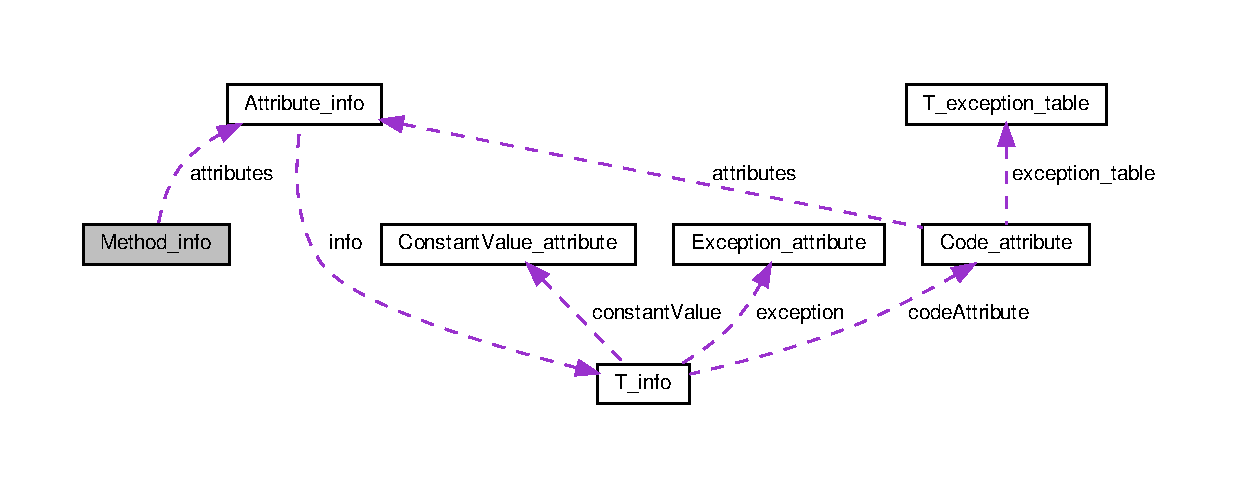
\includegraphics[width=350pt]{structMethod__info__coll__graph}
\end{center}
\end{figure}
\subsection*{Atributos Públicos}
\begin{DoxyCompactItemize}
\item 
uint16\+\_\+t \hyperlink{structMethod__info_a6d6c8c25f4bdb42b77b6a8ac6250398b}{access\+\_\+flags}
\item 
uint16\+\_\+t \hyperlink{structMethod__info_ad1f067bfd8d2d231f598824676dc7851}{name\+\_\+index}
\item 
uint16\+\_\+t \hyperlink{structMethod__info_af713175c97f681296e801e0c11e0ae34}{descriptor\+\_\+index}
\item 
uint16\+\_\+t \hyperlink{structMethod__info_afd638bcc6f20cfa8dd1de8741c8b5493}{attributes\+\_\+count}
\item 
\hyperlink{structAttribute__info}{Attribute\+\_\+info} $\ast$ \hyperlink{structMethod__info_a56fbb565dcff2992d66f57b29774c322}{attributes}
\end{DoxyCompactItemize}


\subsection{Descrição detalhada}
Struct responsável por armazenar os metodos declarados. 

Definido na linha 19 do ficheiro Methods.\+h.



\subsection{Documentação dos dados membro}
\mbox{\Hypertarget{structMethod__info_a6d6c8c25f4bdb42b77b6a8ac6250398b}\label{structMethod__info_a6d6c8c25f4bdb42b77b6a8ac6250398b}} 
\index{Method\+\_\+info@{Method\+\_\+info}!access\+\_\+flags@{access\+\_\+flags}}
\index{access\+\_\+flags@{access\+\_\+flags}!Method\+\_\+info@{Method\+\_\+info}}
\subsubsection{\texorpdfstring{access\+\_\+flags}{access\_flags}}
{\footnotesize\ttfamily uint16\+\_\+t Method\+\_\+info\+::access\+\_\+flags}



Definido na linha 20 do ficheiro Methods.\+h.



Referenciado por gravar\+Arquivo\+Method(), imprimir\+Method(), ler\+Method() e Class\+File\+::verificar\+Main().

\mbox{\Hypertarget{structMethod__info_a56fbb565dcff2992d66f57b29774c322}\label{structMethod__info_a56fbb565dcff2992d66f57b29774c322}} 
\index{Method\+\_\+info@{Method\+\_\+info}!attributes@{attributes}}
\index{attributes@{attributes}!Method\+\_\+info@{Method\+\_\+info}}
\subsubsection{\texorpdfstring{attributes}{attributes}}
{\footnotesize\ttfamily \hyperlink{structAttribute__info}{Attribute\+\_\+info}$\ast$ Method\+\_\+info\+::attributes}



Definido na linha 24 do ficheiro Methods.\+h.



Referenciado por Pilha\+J\+V\+M\+::adicionar\+Frame(), gravar\+Arquivo\+Method(), imprimir\+Method(), Pilha\+J\+V\+M\+::inicializar\+P\+C(), ler\+Method(), Operations\+::lookupswitch(), Pilha\+J\+V\+M\+::\+Pilha\+J\+V\+M() e Operations\+::tableswitch().

\mbox{\Hypertarget{structMethod__info_afd638bcc6f20cfa8dd1de8741c8b5493}\label{structMethod__info_afd638bcc6f20cfa8dd1de8741c8b5493}} 
\index{Method\+\_\+info@{Method\+\_\+info}!attributes\+\_\+count@{attributes\+\_\+count}}
\index{attributes\+\_\+count@{attributes\+\_\+count}!Method\+\_\+info@{Method\+\_\+info}}
\subsubsection{\texorpdfstring{attributes\+\_\+count}{attributes\_count}}
{\footnotesize\ttfamily uint16\+\_\+t Method\+\_\+info\+::attributes\+\_\+count}



Definido na linha 23 do ficheiro Methods.\+h.



Referenciado por gravar\+Arquivo\+Method(), imprimir\+Method() e ler\+Method().

\mbox{\Hypertarget{structMethod__info_af713175c97f681296e801e0c11e0ae34}\label{structMethod__info_af713175c97f681296e801e0c11e0ae34}} 
\index{Method\+\_\+info@{Method\+\_\+info}!descriptor\+\_\+index@{descriptor\+\_\+index}}
\index{descriptor\+\_\+index@{descriptor\+\_\+index}!Method\+\_\+info@{Method\+\_\+info}}
\subsubsection{\texorpdfstring{descriptor\+\_\+index}{descriptor\_index}}
{\footnotesize\ttfamily uint16\+\_\+t Method\+\_\+info\+::descriptor\+\_\+index}



Definido na linha 22 do ficheiro Methods.\+h.



Referenciado por gravar\+Arquivo\+Method(), imprimir\+Method(), ler\+Method(), Class\+File\+::obter\+Class\+That\+Has\+Serached\+Method(), Class\+File\+::obter\+Method() e Class\+File\+::verificar\+Main().

\mbox{\Hypertarget{structMethod__info_ad1f067bfd8d2d231f598824676dc7851}\label{structMethod__info_ad1f067bfd8d2d231f598824676dc7851}} 
\index{Method\+\_\+info@{Method\+\_\+info}!name\+\_\+index@{name\+\_\+index}}
\index{name\+\_\+index@{name\+\_\+index}!Method\+\_\+info@{Method\+\_\+info}}
\subsubsection{\texorpdfstring{name\+\_\+index}{name\_index}}
{\footnotesize\ttfamily uint16\+\_\+t Method\+\_\+info\+::name\+\_\+index}



Definido na linha 21 do ficheiro Methods.\+h.



Referenciado por gravar\+Arquivo\+Method(), imprimir\+Method(), ler\+Method(), Class\+File\+::obter\+Class\+That\+Has\+Serached\+Method(), Class\+File\+::obter\+Method(), Operations\+::putfield(), Class\+File\+::verificar\+Clinit() e Class\+File\+::verificar\+Main().



A documentação para esta estrutura foi gerada a partir do seguinte ficheiro\+:\begin{DoxyCompactItemize}
\item 
include/\hyperlink{Methods_8h}{Methods.\+h}\end{DoxyCompactItemize}

\hypertarget{classMethodArea}{}\section{Referência à classe Method\+Area}
\label{classMethodArea}\index{Method\+Area@{Method\+Area}}


Classe responsável por todas as operações que gerenciam os métodos.  




{\ttfamily \#include $<$Method\+Area.\+h$>$}

\subsection*{Membros públicos}
\begin{DoxyCompactItemize}
\item 
\hyperlink{classMethodArea_a79edf80f07f068f918907d8e2a3508b7}{$\sim$\+Method\+Area} ()
\begin{DoxyCompactList}\small\item\em Destrutor padrão. \end{DoxyCompactList}\item 
\hyperlink{classStaticClass}{Static\+Class} $\ast$ \hyperlink{classMethodArea_a6e5cd27f3133d70a8c56c5daf9190ba6}{carregar\+Class\+Named} (const string \&class\+Name)
\begin{DoxyCompactList}\small\item\em Carrega a classe com o nome dado e a adiciona na área de métodos. \end{DoxyCompactList}\item 
\hyperlink{classStaticClass}{Static\+Class} $\ast$ \hyperlink{classMethodArea_a1fb65cf5f35cadbe2be8ad1aece57025}{get\+Class\+Named} (const string \&class\+Name)
\begin{DoxyCompactList}\small\item\em Busca por uma classe com o nome qualificado passado (e.\+g. java/lang/\+Object). \end{DoxyCompactList}\end{DoxyCompactItemize}
\subsection*{Membros públicos estáticos}
\begin{DoxyCompactItemize}
\item 
static \hyperlink{classMethodArea}{Method\+Area} \& \hyperlink{classMethodArea_ab5fadec94ada20bc6381e7e9ac766cad}{get\+Instance} ()
\begin{DoxyCompactList}\small\item\em Obter a única instância do \hyperlink{classMethodArea}{Method\+Area}. \end{DoxyCompactList}\end{DoxyCompactItemize}
\subsection*{Membros privados}
\begin{DoxyCompactItemize}
\item 
\hyperlink{classMethodArea_a6e9aac39975424e6c0ab3c29535aca75}{Method\+Area} ()
\begin{DoxyCompactList}\small\item\em Construtor padrão. \end{DoxyCompactList}\item 
\hyperlink{classMethodArea_a3a51cf2f998faa40ff46f17019f59e0a}{Method\+Area} (\hyperlink{classMethodArea}{Method\+Area} const \&)
\item 
void \hyperlink{classMethodArea_a02652b16a9bc28ceae405a9959cf4ee8}{operator=} (\hyperlink{classMethodArea}{Method\+Area} const \&)
\item 
bool \hyperlink{classMethodArea_a9e4e378de46c1a9836820d86cd9dadb8}{add\+Class} (\hyperlink{classStaticClass}{Static\+Class} $\ast$class\+File)
\begin{DoxyCompactList}\small\item\em Adiciona uma classe à área de métodos. \end{DoxyCompactList}\end{DoxyCompactItemize}
\subsection*{Atributos Privados}
\begin{DoxyCompactItemize}
\item 
map$<$ string, \hyperlink{classStaticClass}{Static\+Class} $\ast$ $>$ \hyperlink{classMethodArea_a1244d392d351920d754db8c6940dd7aa}{\+\_\+classes}
\end{DoxyCompactItemize}


\subsection{Descrição detalhada}
Classe responsável por todas as operações que gerenciam os métodos. 

Essa classe é um singleton, ou seja, somente existe no máximo 1 instância dela para cada instância da J\+VM. 

Definido na linha 21 do ficheiro Method\+Area.\+h.



\subsection{Documentação dos Construtores \& Destrutor}
\mbox{\Hypertarget{classMethodArea_a79edf80f07f068f918907d8e2a3508b7}\label{classMethodArea_a79edf80f07f068f918907d8e2a3508b7}} 
\index{Method\+Area@{Method\+Area}!````~Method\+Area@{$\sim$\+Method\+Area}}
\index{````~Method\+Area@{$\sim$\+Method\+Area}!Method\+Area@{Method\+Area}}
\subsubsection{\texorpdfstring{$\sim$\+Method\+Area()}{~MethodArea()}}
{\footnotesize\ttfamily Method\+Area\+::$\sim$\+Method\+Area (\begin{DoxyParamCaption}{ }\end{DoxyParamCaption})}



Destrutor padrão. 



Definido na linha 12 do ficheiro Method\+Area.\+cpp.

\mbox{\Hypertarget{classMethodArea_a6e9aac39975424e6c0ab3c29535aca75}\label{classMethodArea_a6e9aac39975424e6c0ab3c29535aca75}} 
\index{Method\+Area@{Method\+Area}!Method\+Area@{Method\+Area}}
\index{Method\+Area@{Method\+Area}!Method\+Area@{Method\+Area}}
\subsubsection{\texorpdfstring{Method\+Area()}{MethodArea()}\hspace{0.1cm}{\footnotesize\ttfamily [1/2]}}
{\footnotesize\ttfamily Method\+Area\+::\+Method\+Area (\begin{DoxyParamCaption}{ }\end{DoxyParamCaption})\hspace{0.3cm}{\ttfamily [private]}}



Construtor padrão. 



Definido na linha 8 do ficheiro Method\+Area.\+cpp.

\mbox{\Hypertarget{classMethodArea_a3a51cf2f998faa40ff46f17019f59e0a}\label{classMethodArea_a3a51cf2f998faa40ff46f17019f59e0a}} 
\index{Method\+Area@{Method\+Area}!Method\+Area@{Method\+Area}}
\index{Method\+Area@{Method\+Area}!Method\+Area@{Method\+Area}}
\subsubsection{\texorpdfstring{Method\+Area()}{MethodArea()}\hspace{0.1cm}{\footnotesize\ttfamily [2/2]}}
{\footnotesize\ttfamily Method\+Area\+::\+Method\+Area (\begin{DoxyParamCaption}\item[{\hyperlink{classMethodArea}{Method\+Area} const \&}]{ }\end{DoxyParamCaption})\hspace{0.3cm}{\ttfamily [private]}}



\subsection{Documentação dos métodos}
\mbox{\Hypertarget{classMethodArea_a9e4e378de46c1a9836820d86cd9dadb8}\label{classMethodArea_a9e4e378de46c1a9836820d86cd9dadb8}} 
\index{Method\+Area@{Method\+Area}!add\+Class@{add\+Class}}
\index{add\+Class@{add\+Class}!Method\+Area@{Method\+Area}}
\subsubsection{\texorpdfstring{add\+Class()}{addClass()}}
{\footnotesize\ttfamily bool Method\+Area\+::add\+Class (\begin{DoxyParamCaption}\item[{\hyperlink{classStaticClass}{Static\+Class} $\ast$}]{class\+File }\end{DoxyParamCaption})\hspace{0.3cm}{\ttfamily [private]}}



Adiciona uma classe à área de métodos. 


\begin{DoxyParams}{Parâmetros}
{\em class\+File} & A classe que será adicionada. \\
\hline
\end{DoxyParams}
\begin{DoxyReturn}{Retorna}
{\ttfamily true} caso a classe foi adicionada, e {\ttfamily false} caso contrário, pois uma classe com o mesmo nome já está adicionada. 
\end{DoxyReturn}


Definido na linha 65 do ficheiro Method\+Area.\+cpp.



Referências \+\_\+classes, Class\+File\+::constant\+\_\+pool, Static\+Class\+::get\+Class\+File(), get\+Formatted\+Constant() e Class\+File\+::this\+\_\+class.



Referenciado por carregar\+Class\+Named().

Grafo de chamadas desta função\+:\nopagebreak
\begin{figure}[H]
\begin{center}
\leavevmode
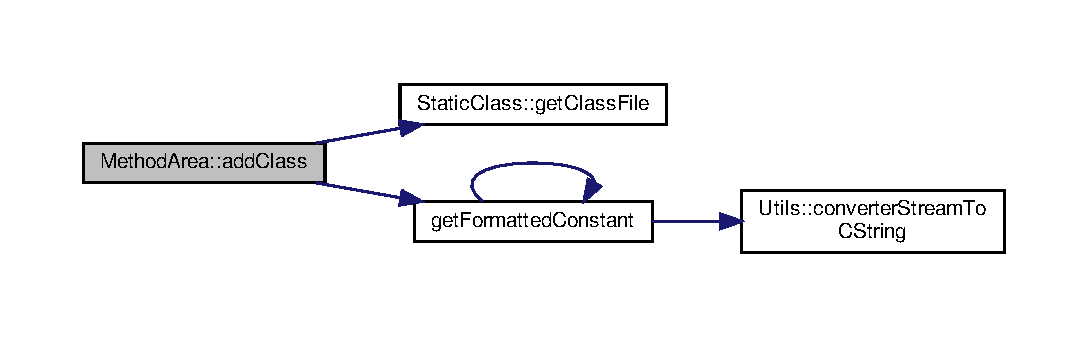
\includegraphics[width=350pt]{classMethodArea_a9e4e378de46c1a9836820d86cd9dadb8_cgraph}
\end{center}
\end{figure}
\mbox{\Hypertarget{classMethodArea_a6e5cd27f3133d70a8c56c5daf9190ba6}\label{classMethodArea_a6e5cd27f3133d70a8c56c5daf9190ba6}} 
\index{Method\+Area@{Method\+Area}!carregar\+Class\+Named@{carregar\+Class\+Named}}
\index{carregar\+Class\+Named@{carregar\+Class\+Named}!Method\+Area@{Method\+Area}}
\subsubsection{\texorpdfstring{carregar\+Class\+Named()}{carregarClassNamed()}}
{\footnotesize\ttfamily \hyperlink{classStaticClass}{Static\+Class} $\ast$ Method\+Area\+::carregar\+Class\+Named (\begin{DoxyParamCaption}\item[{const string \&}]{class\+Name }\end{DoxyParamCaption})}



Carrega a classe com o nome dado e a adiciona na área de métodos. 


\begin{DoxyParams}{Parâmetros}
{\em class\+Name} & O nome da classe (contendo o sufixo .class ou não). \\
\hline
\end{DoxyParams}
\begin{DoxyReturn}{Retorna}
O ponteiro para {\ttfamily \hyperlink{classClassFile}{Class\+File}} da classe carregada. 
\end{DoxyReturn}


Definido na linha 16 do ficheiro Method\+Area.\+cpp.



Referências \+\_\+classes, add\+Class(), Pilha\+J\+V\+M\+::add\+Frame(), get\+Class\+Named(), Pilha\+J\+V\+M\+::get\+Instance(), Leitor\+Exibidor\+::get\+Instance(), Operations\+::get\+Instance(), Leitor\+Exibidor\+::read\+Class\+File() e Operations\+::verificar\+Metodo\+Existe().



Referenciado por Operations\+::anewarray(), Operations\+::checkcast(), Operations\+::func\+\_\+new(), Operations\+::getstatic(), Operations\+::instanceof(), Operations\+::invokeinterface(), Operations\+::invokespecial(), Operations\+::invokestatic(), Operations\+::invokevirtual(), main(), Operations\+::multianewarray(), Frame\+::obter\+Method\+Named() e Operations\+::putstatic().

Grafo de chamadas desta função\+:\nopagebreak
\begin{figure}[H]
\begin{center}
\leavevmode
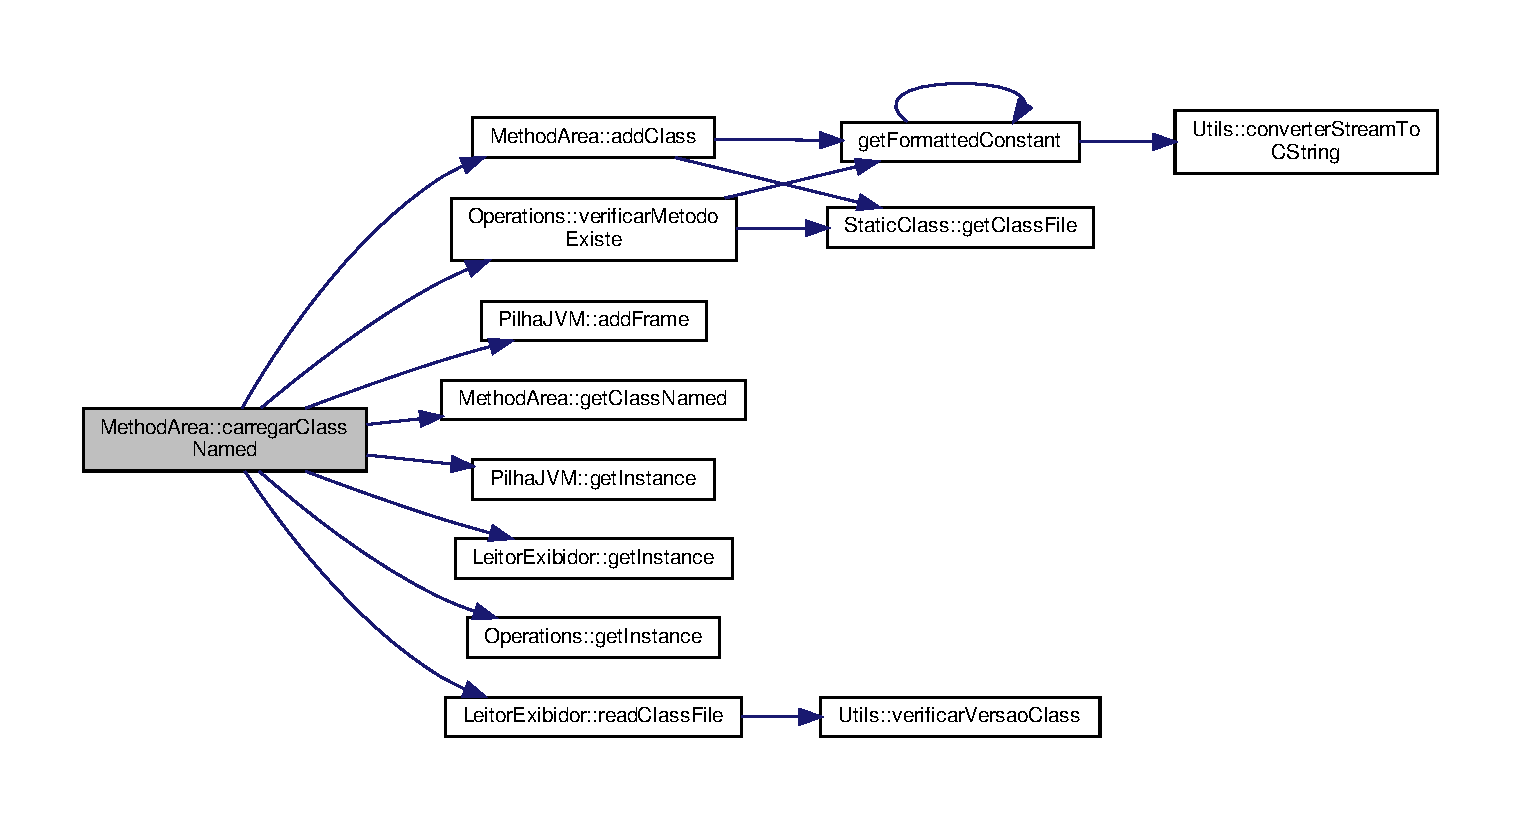
\includegraphics[width=350pt]{classMethodArea_a6e5cd27f3133d70a8c56c5daf9190ba6_cgraph}
\end{center}
\end{figure}
\mbox{\Hypertarget{classMethodArea_a1fb65cf5f35cadbe2be8ad1aece57025}\label{classMethodArea_a1fb65cf5f35cadbe2be8ad1aece57025}} 
\index{Method\+Area@{Method\+Area}!get\+Class\+Named@{get\+Class\+Named}}
\index{get\+Class\+Named@{get\+Class\+Named}!Method\+Area@{Method\+Area}}
\subsubsection{\texorpdfstring{get\+Class\+Named()}{getClassNamed()}}
{\footnotesize\ttfamily \hyperlink{classStaticClass}{Static\+Class} $\ast$ Method\+Area\+::get\+Class\+Named (\begin{DoxyParamCaption}\item[{const string \&}]{class\+Name }\end{DoxyParamCaption})}



Busca por uma classe com o nome qualificado passado (e.\+g. java/lang/\+Object). 


\begin{DoxyParams}{Parâmetros}
{\em class\+Name} & O nome qualificado da classe que será buscado. \\
\hline
\end{DoxyParams}
\begin{DoxyReturn}{Retorna}
Um ponteiro para a classe será retornado caso ela exista, e {\ttfamily N\+U\+LL} caso contrário. 
\end{DoxyReturn}


Definido na linha 55 do ficheiro Method\+Area.\+cpp.



Referências \+\_\+classes.



Referenciado por carregar\+Class\+Named().

\mbox{\Hypertarget{classMethodArea_ab5fadec94ada20bc6381e7e9ac766cad}\label{classMethodArea_ab5fadec94ada20bc6381e7e9ac766cad}} 
\index{Method\+Area@{Method\+Area}!get\+Instance@{get\+Instance}}
\index{get\+Instance@{get\+Instance}!Method\+Area@{Method\+Area}}
\subsubsection{\texorpdfstring{get\+Instance()}{getInstance()}}
{\footnotesize\ttfamily static \hyperlink{classMethodArea}{Method\+Area}\& Method\+Area\+::get\+Instance (\begin{DoxyParamCaption}{ }\end{DoxyParamCaption})\hspace{0.3cm}{\ttfamily [inline]}, {\ttfamily [static]}}



Obter a única instância do \hyperlink{classMethodArea}{Method\+Area}. 

\begin{DoxyReturn}{Retorna}
A instância do \hyperlink{classMethodArea}{Method\+Area}. 
\end{DoxyReturn}


Definido na linha 28 do ficheiro Method\+Area.\+h.



Referenciado por Operations\+::anewarray(), Operations\+::checkcast(), Operations\+::func\+\_\+new(), Operations\+::getstatic(), Operations\+::instanceof(), Operations\+::invokeinterface(), Operations\+::invokespecial(), Operations\+::invokestatic(), Operations\+::invokevirtual(), main(), Operations\+::multianewarray(), Frame\+::obter\+Method\+Named() e Operations\+::putstatic().

\mbox{\Hypertarget{classMethodArea_a02652b16a9bc28ceae405a9959cf4ee8}\label{classMethodArea_a02652b16a9bc28ceae405a9959cf4ee8}} 
\index{Method\+Area@{Method\+Area}!operator=@{operator=}}
\index{operator=@{operator=}!Method\+Area@{Method\+Area}}
\subsubsection{\texorpdfstring{operator=()}{operator=()}}
{\footnotesize\ttfamily void Method\+Area\+::operator= (\begin{DoxyParamCaption}\item[{\hyperlink{classMethodArea}{Method\+Area} const \&}]{ }\end{DoxyParamCaption})\hspace{0.3cm}{\ttfamily [private]}}



\subsection{Documentação dos dados membro}
\mbox{\Hypertarget{classMethodArea_a1244d392d351920d754db8c6940dd7aa}\label{classMethodArea_a1244d392d351920d754db8c6940dd7aa}} 
\index{Method\+Area@{Method\+Area}!\+\_\+classes@{\+\_\+classes}}
\index{\+\_\+classes@{\+\_\+classes}!Method\+Area@{Method\+Area}}
\subsubsection{\texorpdfstring{\+\_\+classes}{\_classes}}
{\footnotesize\ttfamily map$<$string, \hyperlink{classStaticClass}{Static\+Class}$\ast$$>$ Method\+Area\+::\+\_\+classes\hspace{0.3cm}{\ttfamily [private]}}

Um {\ttfamily map} contendo todas as classes presentes na área de métodos.

A chave do map é o nome qualificado da classe, e o valor é um ponteiro para o {\ttfamily \hyperlink{classClassFile}{Class\+File}} correspondente. 

Definido na linha 73 do ficheiro Method\+Area.\+h.



Referenciado por add\+Class(), carregar\+Class\+Named() e get\+Class\+Named().



A documentação para esta classe foi gerada a partir dos seguintes ficheiros\+:\begin{DoxyCompactItemize}
\item 
include/\hyperlink{MethodArea_8h}{Method\+Area.\+h}\item 
src/\hyperlink{MethodArea_8cpp}{Method\+Area.\+cpp}\end{DoxyCompactItemize}

\hypertarget{structN__array}{}\section{Referência à estrutura N\+\_\+array}
\label{structN__array}\index{N\+\_\+array@{N\+\_\+array}}


Agregador de numeros de array Struct responsável armazenar o numero de dims e array.  




{\ttfamily \#include $<$Basic\+Types.\+h$>$}

\subsection*{Atributos Públicos}
\begin{DoxyCompactItemize}
\item 
int $\ast$ \hyperlink{structN__array_ac4bcc6ba8cf97045350bdfbf7d25eaa0}{dims}
\item 
int $\ast$ \hyperlink{structN__array_a86947172fed28646e92c55904ce2907c}{array}
\end{DoxyCompactItemize}


\subsection{Descrição detalhada}
Agregador de numeros de array Struct responsável armazenar o numero de dims e array. 

Definido na linha 73 do ficheiro Basic\+Types.\+h.



\subsection{Documentação dos dados membro}
\mbox{\Hypertarget{structN__array_a86947172fed28646e92c55904ce2907c}\label{structN__array_a86947172fed28646e92c55904ce2907c}} 
\index{N\+\_\+array@{N\+\_\+array}!array@{array}}
\index{array@{array}!N\+\_\+array@{N\+\_\+array}}
\subsubsection{\texorpdfstring{array}{array}}
{\footnotesize\ttfamily int$\ast$ N\+\_\+array\+::array}



Definido na linha 75 do ficheiro Basic\+Types.\+h.



Referenciado por Operations\+::obter\+New\+Multi\+Array() e Operations\+::obter\+Valor().

\mbox{\Hypertarget{structN__array_ac4bcc6ba8cf97045350bdfbf7d25eaa0}\label{structN__array_ac4bcc6ba8cf97045350bdfbf7d25eaa0}} 
\index{N\+\_\+array@{N\+\_\+array}!dims@{dims}}
\index{dims@{dims}!N\+\_\+array@{N\+\_\+array}}
\subsubsection{\texorpdfstring{dims}{dims}}
{\footnotesize\ttfamily int$\ast$ N\+\_\+array\+::dims}



Definido na linha 74 do ficheiro Basic\+Types.\+h.



Referenciado por Operations\+::obter\+New\+Multi\+Array() e Operations\+::obter\+Valor().



A documentação para esta estrutura foi gerada a partir do seguinte ficheiro\+:\begin{DoxyCompactItemize}
\item 
include/\hyperlink{BasicTypes_8h}{Basic\+Types.\+h}\end{DoxyCompactItemize}

\hypertarget{classOperandsStack}{}\section{Referência à classe Operands\+Stack}
\label{classOperandsStack}\index{Operands\+Stack@{Operands\+Stack}}


Classe da pilha de operandos.  




{\ttfamily \#include $<$Operands\+Stack.\+h$>$}

\subsection*{Membros públicos}
\begin{DoxyCompactItemize}
\item 
\hyperlink{classOperandsStack_a5ea2e7d609262388d0d4bc3ba08a2c32}{Operands\+Stack} (int)
\begin{DoxyCompactList}\small\item\em Construtor. \end{DoxyCompactList}\item 
uint8\+\_\+t \hyperlink{classOperandsStack_a8c76f12ad6984b3c5b4ec8807eb63ae3}{desempilha\+Topo\+Tipo} ()
\begin{DoxyCompactList}\small\item\em Recupera o tipo do topo da pilha de operandos. \end{DoxyCompactList}\item 
\hyperlink{BasicTypes_8h_a8132f4f0515064141e31e606660df561}{Element} \hyperlink{classOperandsStack_a184a99d160e17ef874a7b83f0726fb8a}{desempilha\+Topo\+Valor} ()
\begin{DoxyCompactList}\small\item\em Recupera o valor do topo da pilha de operandos. \end{DoxyCompactList}\item 
\hyperlink{BasicTypes_8h_a8132f4f0515064141e31e606660df561}{Element} \hyperlink{classOperandsStack_a3213a1b633149de9332217d403ee84b6}{desempilha} ()
\begin{DoxyCompactList}\small\item\em Desempilha o topo da pilha de operandos e retorna em um elemento de valor. \end{DoxyCompactList}\item 
\hyperlink{BasicTypes_8h_a97b332303b1262282599e6ede0637b82}{Typed\+Element} \hyperlink{classOperandsStack_a9503313a7def4c11fb782d5881e3d6cb}{desempilha\+Typed} ()
\begin{DoxyCompactList}\small\item\em Desempilha o topo da pilha de operandos e retorna em um elemento tipado. \end{DoxyCompactList}\item 
string \hyperlink{classOperandsStack_a32ad6a1ea26c02cf709fed1e86412b4a}{obter\+String} ()
\begin{DoxyCompactList}\small\item\em Retorna o topo da pilha de operandos formatado em uma string. \end{DoxyCompactList}\item 
void \hyperlink{classOperandsStack_a5006a59c2d815e4a24b055e2e4d2e741}{empilhar\+Int} (int x)
\begin{DoxyCompactList}\small\item\em Empilha um valor de tipo inteiro. \end{DoxyCompactList}\item 
void \hyperlink{classOperandsStack_a927ca84358d7e0f45f74d122f9a500d2}{empilhar\+Long} (int64\+\_\+t x)
\begin{DoxyCompactList}\small\item\em Empilha um valor de tipo long. \end{DoxyCompactList}\item 
void \hyperlink{classOperandsStack_aeed478b52748b87ac85db261332b633b}{empilhar\+Float} (float x)
\begin{DoxyCompactList}\small\item\em Empilha um valor de tipo float. \end{DoxyCompactList}\item 
void \hyperlink{classOperandsStack_a45dde91cc54ad980d1cbb7cdb1e084cd}{empilhar\+Double} (double x)
\begin{DoxyCompactList}\small\item\em Empilha um valor de tipo double. \end{DoxyCompactList}\item 
void \hyperlink{classOperandsStack_aca2be3100b76689949f029196a893712}{empilhar\+Bool} (bool x)
\begin{DoxyCompactList}\small\item\em Empilha um valor de tipo bool. \end{DoxyCompactList}\item 
void \hyperlink{classOperandsStack_a47af7d965172984b9cc5c61d8c4c1ce3}{empilhar\+Referencia} (int $\ast$x)
\begin{DoxyCompactList}\small\item\em Empilha um valor de tipo referencia. \end{DoxyCompactList}\item 
void \hyperlink{classOperandsStack_a73960b4536c99847bf4545a45f04f089}{empilhar\+Typed\+Element} (\hyperlink{BasicTypes_8h_a97b332303b1262282599e6ede0637b82}{Typed\+Element} typed\+Element)
\begin{DoxyCompactList}\small\item\em Empilha um elemento tipado, chamando a função adequada ao tipo. \end{DoxyCompactList}\item 
void \hyperlink{classOperandsStack_a50b642d5ff6a7a1f56b8cfc75bde1192}{empilhar} (\hyperlink{BasicTypes_8h_a8132f4f0515064141e31e606660df561}{Element}, uint8\+\_\+t)
\begin{DoxyCompactList}\small\item\em Verifica o tipo do elemento que deve ser empilhado e chama a função adequada. \end{DoxyCompactList}\item 
int \hyperlink{classOperandsStack_a6ea316fc2b2503af2175fada4d4a9741}{obter\+Tamanho} ()
\begin{DoxyCompactList}\small\item\em retorna o tamanho da pilha de operandos \end{DoxyCompactList}\item 
int \hyperlink{classOperandsStack_a834d4e49d01388abf37582f95d66b40e}{obter\+Tamanho\+Maximo\+Pilha} ()
\begin{DoxyCompactList}\small\item\em Retorna o tamanho máximo da pilha de operandos. \end{DoxyCompactList}\item 
bool \hyperlink{classOperandsStack_aa6dbee87661011453ba2c57405bd9a4e}{esta\+Vazia} ()
\begin{DoxyCompactList}\small\item\em Retorna se a pilha está vazia (1) ou não (0) \end{DoxyCompactList}\item 
void \hyperlink{classOperandsStack_a21ecd56a74034dbd8ed6925924cf30e6}{imprimir\+Todas\+Operacoes} ()
\begin{DoxyCompactList}\small\item\em imprimir Todas as Operacoes \end{DoxyCompactList}\end{DoxyCompactItemize}
\subsection*{Atributos Públicos}
\begin{DoxyCompactItemize}
\item 
const int \hyperlink{classOperandsStack_ac17a81af6a26d029042e6c7ad598a538}{max}
\end{DoxyCompactItemize}
\subsection*{Atributos Privados}
\begin{DoxyCompactItemize}
\item 
stack$<$ uint32\+\_\+t $>$ \hyperlink{classOperandsStack_a4d7bd7c3814e216168022849158c733d}{stack\+Elementos}
\item 
stack$<$ uint8\+\_\+t $>$ \hyperlink{classOperandsStack_ad784cabd1a3153f7a870adf07215189a}{stack\+Tipos}
\item 
stack$<$ uint8\+\_\+t $>$ \hyperlink{classOperandsStack_a14729c0f92cf41d1ec65660a7c82555a}{stack\+Tipos\+Reais}
\item 
bool \hyperlink{classOperandsStack_a375521777d4992bc1018eb40da015e70}{type\+Pushed}
\item 
const int \hyperlink{classOperandsStack_aac5d565f6032231c195411ba4d75d571}{real\+Max}
\end{DoxyCompactItemize}
\subsection*{Atributos Privados Estáticos}
\begin{DoxyCompactItemize}
\item 
static const bool \hyperlink{classOperandsStack_a52dbb05109d9b5c88bae178c6fdf00b3}{bits64} = (sizeof(int$\ast$) == 8)
\end{DoxyCompactItemize}


\subsection{Descrição detalhada}
Classe da pilha de operandos. 

Responsável por armazenar e manipular a pilha de operandos 

Definido na linha 32 do ficheiro Operands\+Stack.\+h.



\subsection{Documentação dos Construtores \& Destrutor}
\mbox{\Hypertarget{classOperandsStack_a5ea2e7d609262388d0d4bc3ba08a2c32}\label{classOperandsStack_a5ea2e7d609262388d0d4bc3ba08a2c32}} 
\index{Operands\+Stack@{Operands\+Stack}!Operands\+Stack@{Operands\+Stack}}
\index{Operands\+Stack@{Operands\+Stack}!Operands\+Stack@{Operands\+Stack}}
\subsubsection{\texorpdfstring{Operands\+Stack()}{OperandsStack()}}
{\footnotesize\ttfamily Operands\+Stack\+::\+Operands\+Stack (\begin{DoxyParamCaption}\item[{int}]{max\+Size }\end{DoxyParamCaption})}



Construtor. 

Construtor


\begin{DoxyParams}{Parâmetros}
{\em max\+Size} & Indica tamanho m�ximo da pilha de operandos \\
\hline
\end{DoxyParams}


Definido na linha 11 do ficheiro Operands\+Stack.\+cpp.



Referências type\+Pushed.



\subsection{Documentação dos métodos}
\mbox{\Hypertarget{classOperandsStack_a3213a1b633149de9332217d403ee84b6}\label{classOperandsStack_a3213a1b633149de9332217d403ee84b6}} 
\index{Operands\+Stack@{Operands\+Stack}!desempilha@{desempilha}}
\index{desempilha@{desempilha}!Operands\+Stack@{Operands\+Stack}}
\subsubsection{\texorpdfstring{desempilha()}{desempilha()}}
{\footnotesize\ttfamily element Operands\+Stack\+::desempilha (\begin{DoxyParamCaption}{ }\end{DoxyParamCaption})}



Desempilha o topo da pilha de operandos e retorna em um elemento de valor. 

Retorna e remove topo da pilha de valores e da pop na pilha de tipos 

Definido na linha 52 do ficheiro Operands\+Stack.\+cpp.



Referências bits64, desempilha\+Topo\+Valor(), esta\+Vazia(), stack\+Elementos, stack\+Tipos, stack\+Tipos\+Reais, T\+Y\+P\+E\+\_\+\+D\+O\+U\+B\+LE, T\+Y\+P\+E\+\_\+\+L\+O\+NG e T\+Y\+P\+E\+\_\+\+R\+E\+F\+E\+R\+E\+N\+CE.



Referenciado por Operations\+::aaload(), Operations\+::aastore(), Operations\+::anewarray(), Operations\+::areturn(), Operations\+::arraylength(), Operations\+::athrow(), Operations\+::baload(), Operations\+::bastore(), Operations\+::caload(), Operations\+::castore(), Operations\+::d2f(), Operations\+::d2i(), Operations\+::d2l(), Operations\+::dadd(), Operations\+::daload(), Operations\+::dastore(), Operations\+::dcmpg(), Operations\+::dcmpl(), Operations\+::ddiv(), desempilha\+Typed(), Operations\+::dmul(), Operations\+::dneg(), Operations\+::drem(), Operations\+::dreturn(), Operations\+::dsub(), Operations\+::f2d(), Operations\+::f2i(), Operations\+::f2l(), Operations\+::fadd(), Operations\+::faload(), Operations\+::fastore(), Operations\+::fcmpg(), Operations\+::fcmpl(), Operations\+::fdiv(), Operations\+::fmul(), Operations\+::fneg(), Operations\+::frem(), Operations\+::freturn(), Operations\+::fsub(), Operations\+::func\+\_\+return(), Operations\+::getfield(), Operations\+::i2b(), Operations\+::i2c(), Operations\+::i2d(), Operations\+::i2f(), Operations\+::i2l(), Operations\+::i2s(), Operations\+::iadd(), Operations\+::iaload(), Operations\+::iand(), Operations\+::iastore(), Operations\+::idiv(), Operations\+::if\+\_\+acmpeq(), Operations\+::if\+\_\+acmpne(), Operations\+::if\+\_\+icmpeq(), Operations\+::if\+\_\+icmpge(), Operations\+::if\+\_\+icmpgt(), Operations\+::if\+\_\+icmple(), Operations\+::if\+\_\+icmplt(), Operations\+::if\+\_\+icmpne(), Operations\+::ifeq(), Operations\+::ifge(), Operations\+::ifgt(), Operations\+::ifle(), Operations\+::iflt(), Operations\+::ifne(), Operations\+::ifnonnull(), Operations\+::ifnull(), Operations\+::imul(), Operations\+::ineg(), Operations\+::invokespecial(), Operations\+::ior(), Operations\+::irem(), Operations\+::ireturn(), Operations\+::ishl(), Operations\+::ishr(), Operations\+::isub(), Operations\+::iushr(), Operations\+::ixor(), Operations\+::l2d(), Operations\+::l2f(), Operations\+::l2i(), Operations\+::ladd(), Operations\+::laload(), Operations\+::land(), Operations\+::lastore(), Operations\+::lcmp(), Operations\+::ldiv(), Operations\+::lmul(), Operations\+::lneg(), Operations\+::lookupswitch(), Operations\+::lor(), Operations\+::lrem(), Operations\+::lreturn(), Operations\+::lshl(), Operations\+::lshr(), Operations\+::lsub(), Operations\+::lushr(), Operations\+::lxor(), Operations\+::newarray(), Operations\+::putfield(), Operations\+::saload() e Operations\+::sastore().

Grafo de chamadas desta função\+:\nopagebreak
\begin{figure}[H]
\begin{center}
\leavevmode
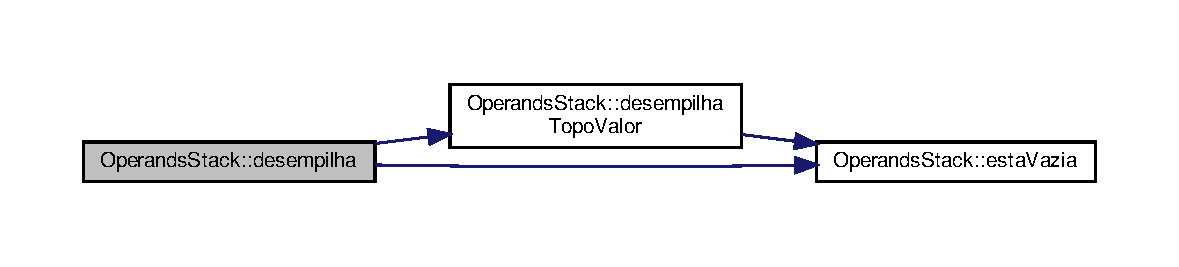
\includegraphics[width=350pt]{classOperandsStack_a3213a1b633149de9332217d403ee84b6_cgraph}
\end{center}
\end{figure}
\mbox{\Hypertarget{classOperandsStack_a8c76f12ad6984b3c5b4ec8807eb63ae3}\label{classOperandsStack_a8c76f12ad6984b3c5b4ec8807eb63ae3}} 
\index{Operands\+Stack@{Operands\+Stack}!desempilha\+Topo\+Tipo@{desempilha\+Topo\+Tipo}}
\index{desempilha\+Topo\+Tipo@{desempilha\+Topo\+Tipo}!Operands\+Stack@{Operands\+Stack}}
\subsubsection{\texorpdfstring{desempilha\+Topo\+Tipo()}{desempilhaTopoTipo()}}
{\footnotesize\ttfamily uint8\+\_\+t Operands\+Stack\+::desempilha\+Topo\+Tipo (\begin{DoxyParamCaption}{ }\end{DoxyParamCaption})}



Recupera o tipo do topo da pilha de operandos. 

Retorna topo da pilha de tipos 

Definido na linha 19 do ficheiro Operands\+Stack.\+cpp.



Referências esta\+Vazia() e stack\+Tipos.



Referenciado por Operations\+::areturn(), Operations\+::astore(), Operations\+::astore\+\_\+0(), Operations\+::astore\+\_\+1(), Operations\+::astore\+\_\+2(), Operations\+::astore\+\_\+3(), Operations\+::athrow(), Operations\+::dadd(), Operations\+::ddiv(), Operations\+::dmul(), Operations\+::dstore(), Operations\+::dstore\+\_\+0(), Operations\+::dstore\+\_\+1(), Operations\+::dstore\+\_\+2(), Operations\+::dstore\+\_\+3(), Operations\+::dsub(), Operations\+::dup2(), Operations\+::dup2\+\_\+x1(), Operations\+::dup2\+\_\+x2(), Operations\+::dup\+\_\+x1(), Operations\+::dup\+\_\+x2(), Operations\+::fadd(), Operations\+::fdiv(), Operations\+::fmul(), Operations\+::fstore(), Operations\+::fstore\+\_\+0(), Operations\+::fstore\+\_\+1(), Operations\+::fstore\+\_\+2(), Operations\+::fstore\+\_\+3(), Operations\+::fsub(), Operations\+::iadd(), Operations\+::idiv(), Operations\+::imul(), Operations\+::istore(), Operations\+::istore\+\_\+0(), Operations\+::istore\+\_\+1(), Operations\+::istore\+\_\+2(), Operations\+::istore\+\_\+3(), Operations\+::isub(), Operations\+::ladd(), Operations\+::ldiv(), Operations\+::lmul(), Operations\+::lstore(), Operations\+::lstore\+\_\+1(), Operations\+::lstore\+\_\+2(), Operations\+::lstore\+\_\+3(), Operations\+::lsub() e obter\+String().

Grafo de chamadas desta função\+:\nopagebreak
\begin{figure}[H]
\begin{center}
\leavevmode
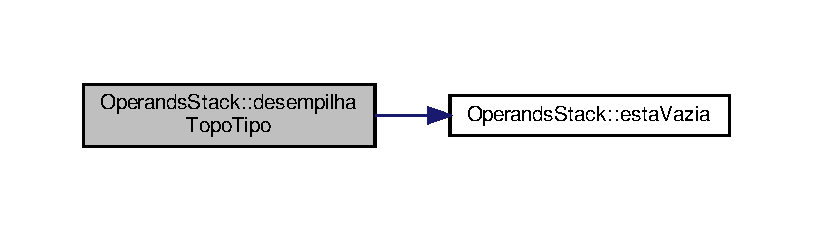
\includegraphics[width=350pt]{classOperandsStack_a8c76f12ad6984b3c5b4ec8807eb63ae3_cgraph}
\end{center}
\end{figure}
\mbox{\Hypertarget{classOperandsStack_a184a99d160e17ef874a7b83f0726fb8a}\label{classOperandsStack_a184a99d160e17ef874a7b83f0726fb8a}} 
\index{Operands\+Stack@{Operands\+Stack}!desempilha\+Topo\+Valor@{desempilha\+Topo\+Valor}}
\index{desempilha\+Topo\+Valor@{desempilha\+Topo\+Valor}!Operands\+Stack@{Operands\+Stack}}
\subsubsection{\texorpdfstring{desempilha\+Topo\+Valor()}{desempilhaTopoValor()}}
{\footnotesize\ttfamily element Operands\+Stack\+::desempilha\+Topo\+Valor (\begin{DoxyParamCaption}{ }\end{DoxyParamCaption})}



Recupera o valor do topo da pilha de operandos. 

Retorna topo da pilha de valores 

Definido na linha 26 do ficheiro Operands\+Stack.\+cpp.



Referências bits64, esta\+Vazia(), element\+\_\+u\+::i, element\+\_\+u\+::l, stack\+Elementos, stack\+Tipos, T\+Y\+P\+E\+\_\+\+D\+O\+U\+B\+LE, T\+Y\+P\+E\+\_\+\+L\+O\+NG e T\+Y\+P\+E\+\_\+\+R\+E\+F\+E\+R\+E\+N\+CE.



Referenciado por desempilha() e obter\+String().

Grafo de chamadas desta função\+:\nopagebreak
\begin{figure}[H]
\begin{center}
\leavevmode
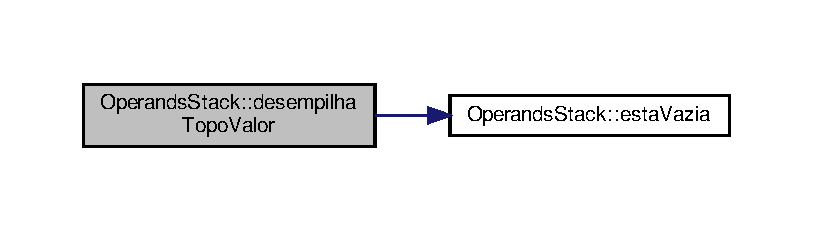
\includegraphics[width=350pt]{classOperandsStack_a184a99d160e17ef874a7b83f0726fb8a_cgraph}
\end{center}
\end{figure}
\mbox{\Hypertarget{classOperandsStack_a9503313a7def4c11fb782d5881e3d6cb}\label{classOperandsStack_a9503313a7def4c11fb782d5881e3d6cb}} 
\index{Operands\+Stack@{Operands\+Stack}!desempilha\+Typed@{desempilha\+Typed}}
\index{desempilha\+Typed@{desempilha\+Typed}!Operands\+Stack@{Operands\+Stack}}
\subsubsection{\texorpdfstring{desempilha\+Typed()}{desempilhaTyped()}}
{\footnotesize\ttfamily element Operands\+Stack\+::desempilha\+Typed (\begin{DoxyParamCaption}{ }\end{DoxyParamCaption})}



Desempilha o topo da pilha de operandos e retorna em um elemento tipado. 

Retorna estrutura com valor e tipo associados e da pop na pilha de valores e na de tipos 

Definido na linha 81 do ficheiro Operands\+Stack.\+cpp.



Referências desempilha(), typed\+Element\+\_\+s\+::real\+Type, stack\+Tipos, stack\+Tipos\+Reais, typed\+Element\+\_\+s\+::type e typed\+Element\+\_\+s\+::value.



Referenciado por Operations\+::astore(), Operations\+::astore\+\_\+0(), Operations\+::astore\+\_\+1(), Operations\+::astore\+\_\+2(), Operations\+::astore\+\_\+3(), Operations\+::dstore(), Operations\+::dstore\+\_\+0(), Operations\+::dstore\+\_\+1(), Operations\+::dstore\+\_\+2(), Operations\+::dstore\+\_\+3(), Operations\+::dup(), Operations\+::dup2(), Operations\+::dup2\+\_\+x1(), Operations\+::dup2\+\_\+x2(), Operations\+::dup\+\_\+x1(), Operations\+::dup\+\_\+x2(), Operations\+::fstore(), Operations\+::fstore\+\_\+0(), Operations\+::fstore\+\_\+1(), Operations\+::fstore\+\_\+2(), Operations\+::fstore\+\_\+3(), imprimir\+Todas\+Operacoes(), Operations\+::invokeinterface(), Operations\+::invokespecial(), Operations\+::invokestatic(), Operations\+::invokevirtual(), Operations\+::istore(), Operations\+::istore\+\_\+0(), Operations\+::istore\+\_\+1(), Operations\+::istore\+\_\+2(), Operations\+::istore\+\_\+3(), Operations\+::lstore(), Operations\+::lstore\+\_\+0(), Operations\+::lstore\+\_\+1(), Operations\+::lstore\+\_\+2(), Operations\+::lstore\+\_\+3(), Operations\+::multianewarray(), Operations\+::pop(), Operations\+::pop2(), Operations\+::putfield(), Operations\+::putstatic(), Operations\+::swap() e Operations\+::tableswitch().

Grafo de chamadas desta função\+:\nopagebreak
\begin{figure}[H]
\begin{center}
\leavevmode
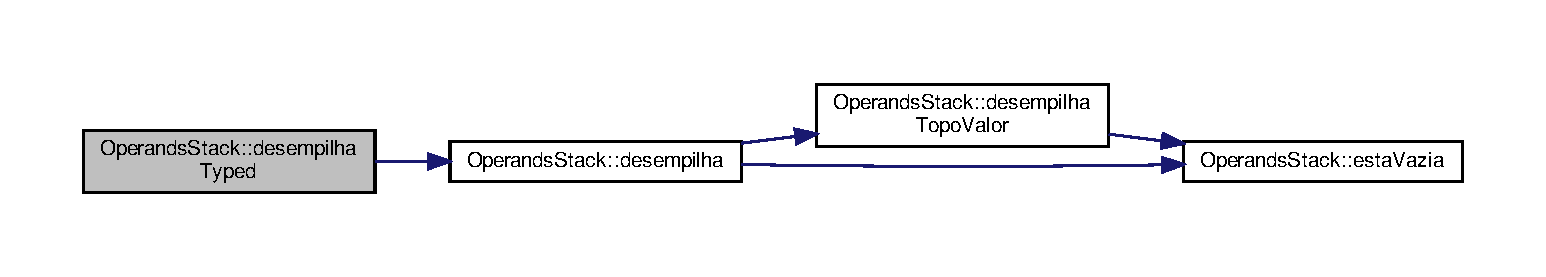
\includegraphics[width=350pt]{classOperandsStack_a9503313a7def4c11fb782d5881e3d6cb_cgraph}
\end{center}
\end{figure}
\mbox{\Hypertarget{classOperandsStack_a50b642d5ff6a7a1f56b8cfc75bde1192}\label{classOperandsStack_a50b642d5ff6a7a1f56b8cfc75bde1192}} 
\index{Operands\+Stack@{Operands\+Stack}!empilhar@{empilhar}}
\index{empilhar@{empilhar}!Operands\+Stack@{Operands\+Stack}}
\subsubsection{\texorpdfstring{empilhar()}{empilhar()}}
{\footnotesize\ttfamily void Operands\+Stack\+::empilhar (\begin{DoxyParamCaption}\item[{\hyperlink{BasicTypes_8h_a8132f4f0515064141e31e606660df561}{Element}}]{element,  }\item[{uint8\+\_\+t}]{tipo }\end{DoxyParamCaption})}



Verifica o tipo do elemento que deve ser empilhado e chama a função adequada. 

Chama a função para empilhar de acordo com o tipo do elemento recebido


\begin{DoxyParams}{Parâmetros}
{\em element} & Elemento a ser empilhado \\
\hline
{\em tipo} & Tipo do elemento a ser empilhado \\
\hline
\end{DoxyParams}


Definido na linha 285 do ficheiro Operands\+Stack.\+cpp.



Referências element\+\_\+u\+::b, element\+\_\+u\+::d, empilhar\+Double(), empilhar\+Float(), empilhar\+Int(), empilhar\+Referencia(), element\+\_\+u\+::f, element\+\_\+u\+::i, element\+\_\+u\+::pi, T\+Y\+P\+E\+\_\+\+B\+O\+OL, T\+Y\+P\+E\+\_\+\+D\+O\+U\+B\+LE, T\+Y\+P\+E\+\_\+\+F\+L\+O\+AT, T\+Y\+P\+E\+\_\+\+I\+NT, T\+Y\+P\+E\+\_\+\+L\+O\+NG e T\+Y\+P\+E\+\_\+\+R\+E\+F\+E\+R\+E\+N\+CE.



Referenciado por Operations\+::athrow(), Operations\+::d2l(), empilhar\+Typed\+Element(), Operations\+::f2l(), Operations\+::i2l(), Operations\+::ior(), Operations\+::ixor(), Operations\+::l2f(), Operations\+::l2i(), Operations\+::ldc(), Operations\+::lor() e Operations\+::lxor().

Grafo de chamadas desta função\+:\nopagebreak
\begin{figure}[H]
\begin{center}
\leavevmode
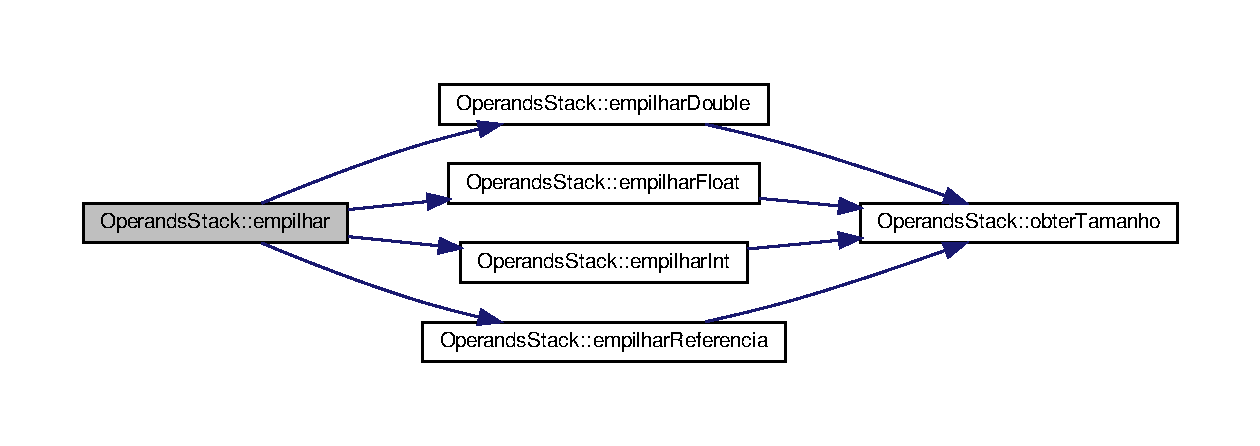
\includegraphics[width=350pt]{classOperandsStack_a50b642d5ff6a7a1f56b8cfc75bde1192_cgraph}
\end{center}
\end{figure}
\mbox{\Hypertarget{classOperandsStack_aca2be3100b76689949f029196a893712}\label{classOperandsStack_aca2be3100b76689949f029196a893712}} 
\index{Operands\+Stack@{Operands\+Stack}!empilhar\+Bool@{empilhar\+Bool}}
\index{empilhar\+Bool@{empilhar\+Bool}!Operands\+Stack@{Operands\+Stack}}
\subsubsection{\texorpdfstring{empilhar\+Bool()}{empilharBool()}}
{\footnotesize\ttfamily void Operands\+Stack\+::empilhar\+Bool (\begin{DoxyParamCaption}\item[{bool}]{x }\end{DoxyParamCaption})}



Empilha um valor de tipo bool. 

Empilha um bool na pilha de valores e seu tipo na pilha de tipos


\begin{DoxyParams}{Parâmetros}
{\em x} & Valor a ser empilhado \\
\hline
\end{DoxyParams}


Definido na linha 222 do ficheiro Operands\+Stack.\+cpp.



Referências element\+\_\+u\+::b, element\+\_\+u\+::i, max, obter\+Tamanho(), R\+T\+\_\+\+B\+O\+OL, stack\+Elementos, stack\+Tipos, stack\+Tipos\+Reais, T\+Y\+P\+E\+\_\+\+B\+O\+OL e type\+Pushed.



Referenciado por Operations\+::jsr\+\_\+w().

Grafo de chamadas desta função\+:\nopagebreak
\begin{figure}[H]
\begin{center}
\leavevmode
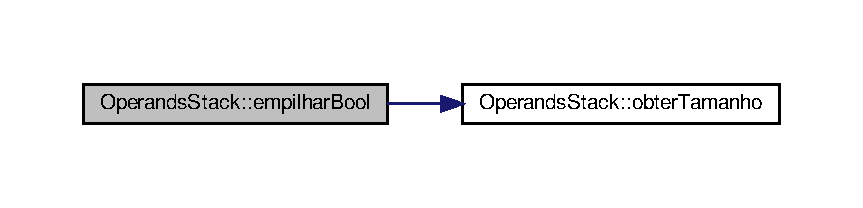
\includegraphics[width=350pt]{classOperandsStack_aca2be3100b76689949f029196a893712_cgraph}
\end{center}
\end{figure}
\mbox{\Hypertarget{classOperandsStack_a45dde91cc54ad980d1cbb7cdb1e084cd}\label{classOperandsStack_a45dde91cc54ad980d1cbb7cdb1e084cd}} 
\index{Operands\+Stack@{Operands\+Stack}!empilhar\+Double@{empilhar\+Double}}
\index{empilhar\+Double@{empilhar\+Double}!Operands\+Stack@{Operands\+Stack}}
\subsubsection{\texorpdfstring{empilhar\+Double()}{empilharDouble()}}
{\footnotesize\ttfamily void Operands\+Stack\+::empilhar\+Double (\begin{DoxyParamCaption}\item[{double}]{x }\end{DoxyParamCaption})}



Empilha um valor de tipo double. 

Empilha um double na pilha de valores e seu tipo na pilha de tipos


\begin{DoxyParams}{Parâmetros}
{\em x} & Valor a ser empilhado \\
\hline
\end{DoxyParams}


Definido na linha 168 do ficheiro Operands\+Stack.\+cpp.



Referências element\+\_\+u\+::d, element\+\_\+u\+::i, element\+\_\+u\+::l, max, obter\+Tamanho(), R\+T\+\_\+\+D\+O\+U\+B\+LE, stack\+Elementos, stack\+Tipos, stack\+Tipos\+Reais, T\+Y\+P\+E\+\_\+\+D\+O\+U\+B\+LE e type\+Pushed.



Referenciado por Operations\+::dconst\+\_\+0(), Operations\+::dconst\+\_\+1(), Operations\+::dload(), Operations\+::dload\+\_\+n(), Operations\+::dreturn(), empilhar(), Operations\+::f2d(), Operations\+::i2d(), Operations\+::l2d() e Operations\+::ldc2\+\_\+w().

Grafo de chamadas desta função\+:\nopagebreak
\begin{figure}[H]
\begin{center}
\leavevmode
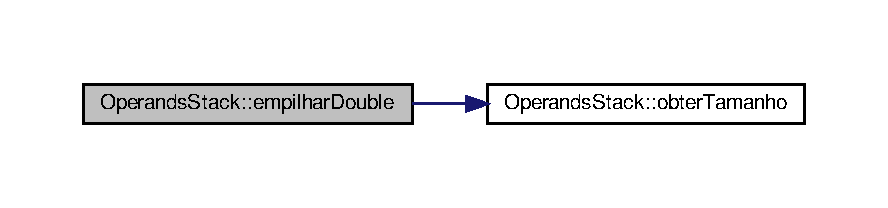
\includegraphics[width=350pt]{classOperandsStack_a45dde91cc54ad980d1cbb7cdb1e084cd_cgraph}
\end{center}
\end{figure}
\mbox{\Hypertarget{classOperandsStack_aeed478b52748b87ac85db261332b633b}\label{classOperandsStack_aeed478b52748b87ac85db261332b633b}} 
\index{Operands\+Stack@{Operands\+Stack}!empilhar\+Float@{empilhar\+Float}}
\index{empilhar\+Float@{empilhar\+Float}!Operands\+Stack@{Operands\+Stack}}
\subsubsection{\texorpdfstring{empilhar\+Float()}{empilharFloat()}}
{\footnotesize\ttfamily void Operands\+Stack\+::empilhar\+Float (\begin{DoxyParamCaption}\item[{float}]{x }\end{DoxyParamCaption})}



Empilha um valor de tipo float. 

Empilha um float na pilha de valores e seu tipo na pilha de tipos


\begin{DoxyParams}{Parâmetros}
{\em x} & Valor a ser empilhado \\
\hline
\end{DoxyParams}


Definido na linha 145 do ficheiro Operands\+Stack.\+cpp.



Referências element\+\_\+u\+::f, element\+\_\+u\+::i, max, obter\+Tamanho(), R\+T\+\_\+\+F\+L\+O\+AT, stack\+Elementos, stack\+Tipos, stack\+Tipos\+Reais, T\+Y\+P\+E\+\_\+\+F\+L\+O\+AT e type\+Pushed.



Referenciado por Operations\+::d2f(), empilhar(), Operations\+::fconst\+\_\+0(), Operations\+::fconst\+\_\+1(), Operations\+::fconst\+\_\+2(), Operations\+::fload(), Operations\+::fload\+\_\+n(), Operations\+::freturn() e Operations\+::i2f().

Grafo de chamadas desta função\+:\nopagebreak
\begin{figure}[H]
\begin{center}
\leavevmode
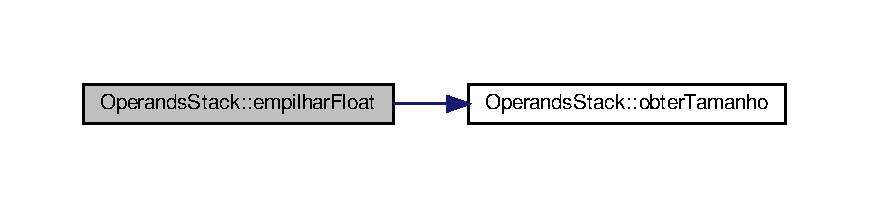
\includegraphics[width=350pt]{classOperandsStack_aeed478b52748b87ac85db261332b633b_cgraph}
\end{center}
\end{figure}
\mbox{\Hypertarget{classOperandsStack_a5006a59c2d815e4a24b055e2e4d2e741}\label{classOperandsStack_a5006a59c2d815e4a24b055e2e4d2e741}} 
\index{Operands\+Stack@{Operands\+Stack}!empilhar\+Int@{empilhar\+Int}}
\index{empilhar\+Int@{empilhar\+Int}!Operands\+Stack@{Operands\+Stack}}
\subsubsection{\texorpdfstring{empilhar\+Int()}{empilharInt()}}
{\footnotesize\ttfamily void Operands\+Stack\+::empilhar\+Int (\begin{DoxyParamCaption}\item[{int}]{x }\end{DoxyParamCaption})}



Empilha um valor de tipo inteiro. 

Empilha um int na pilha de valores e seu tipo na pilha de tipos


\begin{DoxyParams}{Parâmetros}
{\em x} & Valor a ser empilhado \\
\hline
\end{DoxyParams}


Definido na linha 124 do ficheiro Operands\+Stack.\+cpp.



Referências max, obter\+Tamanho(), R\+T\+\_\+\+I\+NT, stack\+Elementos, stack\+Tipos, stack\+Tipos\+Reais, T\+Y\+P\+E\+\_\+\+I\+NT e type\+Pushed.



Referenciado por Operations\+::arraylength(), Operations\+::bipush(), Operations\+::caload(), Operations\+::d2i(), Operations\+::dcmpg(), Operations\+::dcmpl(), empilhar(), Operations\+::f2i(), Operations\+::fcmpg(), Operations\+::fcmpl(), Operations\+::i2b(), Operations\+::iaload(), Operations\+::iconst\+\_\+0(), Operations\+::iconst\+\_\+1(), Operations\+::iconst\+\_\+2(), Operations\+::iconst\+\_\+3(), Operations\+::iconst\+\_\+4(), Operations\+::iconst\+\_\+5(), Operations\+::iconst\+\_\+m1(), Operations\+::iload(), Operations\+::iload\+\_\+0(), Operations\+::iload\+\_\+1(), Operations\+::iload\+\_\+2(), Operations\+::iload\+\_\+3(), Operations\+::ireturn(), Operations\+::lcmp(), Operations\+::ldc\+\_\+w() e Operations\+::sipush().

Grafo de chamadas desta função\+:\nopagebreak
\begin{figure}[H]
\begin{center}
\leavevmode
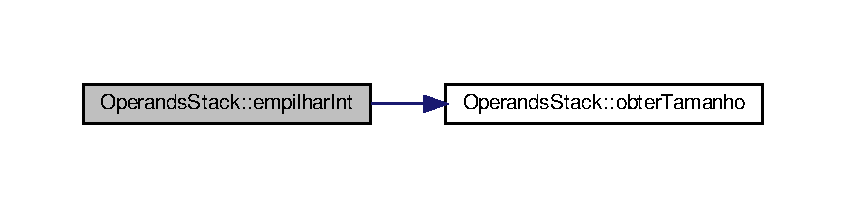
\includegraphics[width=350pt]{classOperandsStack_a5006a59c2d815e4a24b055e2e4d2e741_cgraph}
\end{center}
\end{figure}
\mbox{\Hypertarget{classOperandsStack_a927ca84358d7e0f45f74d122f9a500d2}\label{classOperandsStack_a927ca84358d7e0f45f74d122f9a500d2}} 
\index{Operands\+Stack@{Operands\+Stack}!empilhar\+Long@{empilhar\+Long}}
\index{empilhar\+Long@{empilhar\+Long}!Operands\+Stack@{Operands\+Stack}}
\subsubsection{\texorpdfstring{empilhar\+Long()}{empilharLong()}}
{\footnotesize\ttfamily void Operands\+Stack\+::empilhar\+Long (\begin{DoxyParamCaption}\item[{int64\+\_\+t}]{x }\end{DoxyParamCaption})}



Empilha um valor de tipo long. 

Empilha um long na pilha de valores e seu tipo na pilha de tipos


\begin{DoxyParams}{Parâmetros}
{\em x} & Valor a ser empilhado \\
\hline
\end{DoxyParams}


Definido na linha 196 do ficheiro Operands\+Stack.\+cpp.



Referências max, obter\+Tamanho(), R\+T\+\_\+\+L\+O\+NG, stack\+Elementos, stack\+Tipos, stack\+Tipos\+Reais, T\+Y\+P\+E\+\_\+\+L\+O\+NG e type\+Pushed.



Referenciado por Operations\+::lconst\+\_\+0(), Operations\+::lconst\+\_\+1(), Operations\+::ldc2\+\_\+w(), Operations\+::lload(), Operations\+::lload\+\_\+n() e Operations\+::lreturn().

Grafo de chamadas desta função\+:\nopagebreak
\begin{figure}[H]
\begin{center}
\leavevmode
\includegraphics[width=350pt]{classOperandsStack_a927ca84358d7e0f45f74d122f9a500d2_cgraph}
\end{center}
\end{figure}
\mbox{\Hypertarget{classOperandsStack_a47af7d965172984b9cc5c61d8c4c1ce3}\label{classOperandsStack_a47af7d965172984b9cc5c61d8c4c1ce3}} 
\index{Operands\+Stack@{Operands\+Stack}!empilhar\+Referencia@{empilhar\+Referencia}}
\index{empilhar\+Referencia@{empilhar\+Referencia}!Operands\+Stack@{Operands\+Stack}}
\subsubsection{\texorpdfstring{empilhar\+Referencia()}{empilharReferencia()}}
{\footnotesize\ttfamily void Operands\+Stack\+::empilhar\+Referencia (\begin{DoxyParamCaption}\item[{int $\ast$}]{x }\end{DoxyParamCaption})}



Empilha um valor de tipo referencia. 

Empilha uma referencia na pilha de valores e seu tipo na pilha de tipos


\begin{DoxyParams}{Parâmetros}
{\em x} & Referencia a ser empilhada \\
\hline
\end{DoxyParams}


Definido na linha 246 do ficheiro Operands\+Stack.\+cpp.



Referências bits64, element\+\_\+u\+::i, element\+\_\+u\+::l, max, obter\+Tamanho(), element\+\_\+u\+::pi, R\+T\+\_\+\+R\+E\+F\+E\+R\+E\+N\+CE, stack\+Elementos, stack\+Tipos, stack\+Tipos\+Reais, T\+Y\+P\+E\+\_\+\+R\+E\+F\+E\+R\+E\+N\+CE e type\+Pushed.



Referenciado por Operations\+::aconst\+\_\+null(), Operations\+::aload(), Operations\+::aload\+\_\+n(), Operations\+::anewarray(), Operations\+::areturn(), empilhar(), Operations\+::func\+\_\+new(), Operations\+::jsr(), Operations\+::ldc(), Operations\+::ldc\+\_\+w() e Operations\+::newarray().

Grafo de chamadas desta função\+:\nopagebreak
\begin{figure}[H]
\begin{center}
\leavevmode
\includegraphics[width=350pt]{classOperandsStack_a47af7d965172984b9cc5c61d8c4c1ce3_cgraph}
\end{center}
\end{figure}
\mbox{\Hypertarget{classOperandsStack_a73960b4536c99847bf4545a45f04f089}\label{classOperandsStack_a73960b4536c99847bf4545a45f04f089}} 
\index{Operands\+Stack@{Operands\+Stack}!empilhar\+Typed\+Element@{empilhar\+Typed\+Element}}
\index{empilhar\+Typed\+Element@{empilhar\+Typed\+Element}!Operands\+Stack@{Operands\+Stack}}
\subsubsection{\texorpdfstring{empilhar\+Typed\+Element()}{empilharTypedElement()}}
{\footnotesize\ttfamily void Operands\+Stack\+::empilhar\+Typed\+Element (\begin{DoxyParamCaption}\item[{\hyperlink{BasicTypes_8h_a97b332303b1262282599e6ede0637b82}{Typed\+Element}}]{typed\+Element }\end{DoxyParamCaption})}



Empilha um elemento tipado, chamando a função adequada ao tipo. 

Empilha valor e tipo de estrutura com valor e tipo associados


\begin{DoxyParams}{Parâmetros}
{\em typed\+Element} & Elemento tipado a ser empilhado \\
\hline
\end{DoxyParams}


Definido na linha 276 do ficheiro Operands\+Stack.\+cpp.



Referências empilhar(), typed\+Element\+\_\+s\+::real\+Type, stack\+Tipos\+Reais, typed\+Element\+\_\+s\+::type, type\+Pushed e typed\+Element\+\_\+s\+::value.



Referenciado por Operations\+::aaload(), Operations\+::baload(), Operations\+::dadd(), Operations\+::daload(), Operations\+::ddiv(), Operations\+::dmul(), Operations\+::dneg(), Operations\+::drem(), Operations\+::dsub(), Operations\+::dup(), Operations\+::dup2(), Operations\+::dup2\+\_\+x1(), Operations\+::dup2\+\_\+x2(), Operations\+::dup\+\_\+x1(), Operations\+::dup\+\_\+x2(), Operations\+::fadd(), Operations\+::faload(), Operations\+::fdiv(), Operations\+::fmul(), Operations\+::fneg(), Operations\+::frem(), Operations\+::fsub(), Operations\+::getfield(), Operations\+::getstatic(), Operations\+::i2c(), Operations\+::i2s(), Operations\+::iadd(), Operations\+::iand(), Operations\+::idiv(), imprimir\+Todas\+Operacoes(), Operations\+::imul(), Operations\+::ineg(), Operations\+::invokeinterface(), Operations\+::invokespecial(), Operations\+::invokestatic(), Operations\+::invokevirtual(), Operations\+::irem(), Operations\+::ishl(), Operations\+::ishr(), Operations\+::isub(), Operations\+::iushr(), Operations\+::ladd(), Operations\+::laload(), Operations\+::land(), Operations\+::ldiv(), Operations\+::lmul(), Operations\+::lneg(), Operations\+::lrem(), Operations\+::lshl(), Operations\+::lshr(), Operations\+::lsub(), Operations\+::lushr(), Operations\+::multianewarray(), Operations\+::saload() e Operations\+::swap().

Grafo de chamadas desta função\+:\nopagebreak
\begin{figure}[H]
\begin{center}
\leavevmode
\includegraphics[width=350pt]{classOperandsStack_a73960b4536c99847bf4545a45f04f089_cgraph}
\end{center}
\end{figure}
\mbox{\Hypertarget{classOperandsStack_aa6dbee87661011453ba2c57405bd9a4e}\label{classOperandsStack_aa6dbee87661011453ba2c57405bd9a4e}} 
\index{Operands\+Stack@{Operands\+Stack}!esta\+Vazia@{esta\+Vazia}}
\index{esta\+Vazia@{esta\+Vazia}!Operands\+Stack@{Operands\+Stack}}
\subsubsection{\texorpdfstring{esta\+Vazia()}{estaVazia()}}
{\footnotesize\ttfamily bool Operands\+Stack\+::esta\+Vazia (\begin{DoxyParamCaption}{ }\end{DoxyParamCaption})}



Retorna se a pilha está vazia (1) ou não (0) 

returna 1 se a pilha de valores estiver vazia, 0 caso contr�rio 

Definido na linha 343 do ficheiro Operands\+Stack.\+cpp.



Referências stack\+Elementos.



Referenciado por Operations\+::areturn(), Operations\+::athrow(), desempilha(), desempilha\+Topo\+Tipo(), desempilha\+Topo\+Valor(), Operations\+::dreturn(), Operations\+::freturn(), Operations\+::func\+\_\+return(), imprimir\+Todas\+Operacoes(), Operations\+::ireturn() e Operations\+::lreturn().

\mbox{\Hypertarget{classOperandsStack_a21ecd56a74034dbd8ed6925924cf30e6}\label{classOperandsStack_a21ecd56a74034dbd8ed6925924cf30e6}} 
\index{Operands\+Stack@{Operands\+Stack}!imprimir\+Todas\+Operacoes@{imprimir\+Todas\+Operacoes}}
\index{imprimir\+Todas\+Operacoes@{imprimir\+Todas\+Operacoes}!Operands\+Stack@{Operands\+Stack}}
\subsubsection{\texorpdfstring{imprimir\+Todas\+Operacoes()}{imprimirTodasOperacoes()}}
{\footnotesize\ttfamily void Operands\+Stack\+::imprimir\+Todas\+Operacoes (\begin{DoxyParamCaption}{ }\end{DoxyParamCaption})}



imprimir Todas as Operacoes 

Percorre e imprime toda a pilha de operandos 

Definido na linha 327 do ficheiro Operands\+Stack.\+cpp.



Referências desempilha\+Typed(), empilhar\+Typed\+Element(), esta\+Vazia(), max e obter\+String().

Grafo de chamadas desta função\+:\nopagebreak
\begin{figure}[H]
\begin{center}
\leavevmode
\includegraphics[width=350pt]{classOperandsStack_a21ecd56a74034dbd8ed6925924cf30e6_cgraph}
\end{center}
\end{figure}
\mbox{\Hypertarget{classOperandsStack_a32ad6a1ea26c02cf709fed1e86412b4a}\label{classOperandsStack_a32ad6a1ea26c02cf709fed1e86412b4a}} 
\index{Operands\+Stack@{Operands\+Stack}!obter\+String@{obter\+String}}
\index{obter\+String@{obter\+String}!Operands\+Stack@{Operands\+Stack}}
\subsubsection{\texorpdfstring{obter\+String()}{obterString()}}
{\footnotesize\ttfamily string Operands\+Stack\+::obter\+String (\begin{DoxyParamCaption}{ }\end{DoxyParamCaption})}



Retorna o topo da pilha de operandos formatado em uma string. 

Auxiliar do print\+All, imprime a string correspondente ao tipo do elemento 

Definido na linha 93 do ficheiro Operands\+Stack.\+cpp.



Referências element\+\_\+u\+::b, element\+\_\+u\+::d, desempilha\+Topo\+Tipo(), desempilha\+Topo\+Valor(), element\+\_\+u\+::f, element\+\_\+u\+::pi, T\+Y\+P\+E\+\_\+\+B\+O\+OL, T\+Y\+P\+E\+\_\+\+D\+O\+U\+B\+LE, T\+Y\+P\+E\+\_\+\+F\+L\+O\+AT, T\+Y\+P\+E\+\_\+\+I\+NT, T\+Y\+P\+E\+\_\+\+L\+O\+NG e T\+Y\+P\+E\+\_\+\+R\+E\+F\+E\+R\+E\+N\+CE.



Referenciado por imprimir\+Todas\+Operacoes().

Grafo de chamadas desta função\+:\nopagebreak
\begin{figure}[H]
\begin{center}
\leavevmode
\includegraphics[width=350pt]{classOperandsStack_a32ad6a1ea26c02cf709fed1e86412b4a_cgraph}
\end{center}
\end{figure}
\mbox{\Hypertarget{classOperandsStack_a6ea316fc2b2503af2175fada4d4a9741}\label{classOperandsStack_a6ea316fc2b2503af2175fada4d4a9741}} 
\index{Operands\+Stack@{Operands\+Stack}!obter\+Tamanho@{obter\+Tamanho}}
\index{obter\+Tamanho@{obter\+Tamanho}!Operands\+Stack@{Operands\+Stack}}
\subsubsection{\texorpdfstring{obter\+Tamanho()}{obterTamanho()}}
{\footnotesize\ttfamily int Operands\+Stack\+::obter\+Tamanho (\begin{DoxyParamCaption}{ }\end{DoxyParamCaption})}



retorna o tamanho da pilha de operandos 

Retorna o tamanho da pilha de valores 

Definido na linha 320 do ficheiro Operands\+Stack.\+cpp.



Referências stack\+Elementos.



Referenciado por empilhar\+Bool(), empilhar\+Double(), empilhar\+Float(), empilhar\+Int(), empilhar\+Long() e empilhar\+Referencia().

\mbox{\Hypertarget{classOperandsStack_a834d4e49d01388abf37582f95d66b40e}\label{classOperandsStack_a834d4e49d01388abf37582f95d66b40e}} 
\index{Operands\+Stack@{Operands\+Stack}!obter\+Tamanho\+Maximo\+Pilha@{obter\+Tamanho\+Maximo\+Pilha}}
\index{obter\+Tamanho\+Maximo\+Pilha@{obter\+Tamanho\+Maximo\+Pilha}!Operands\+Stack@{Operands\+Stack}}
\subsubsection{\texorpdfstring{obter\+Tamanho\+Maximo\+Pilha()}{obterTamanhoMaximoPilha()}}
{\footnotesize\ttfamily int Operands\+Stack\+::obter\+Tamanho\+Maximo\+Pilha (\begin{DoxyParamCaption}{ }\end{DoxyParamCaption})}



Retorna o tamanho máximo da pilha de operandos. 

Retorna valor m�ximo da pilha de operandos 

Definido na linha 313 do ficheiro Operands\+Stack.\+cpp.



Referências real\+Max.



\subsection{Documentação dos dados membro}
\mbox{\Hypertarget{classOperandsStack_a52dbb05109d9b5c88bae178c6fdf00b3}\label{classOperandsStack_a52dbb05109d9b5c88bae178c6fdf00b3}} 
\index{Operands\+Stack@{Operands\+Stack}!bits64@{bits64}}
\index{bits64@{bits64}!Operands\+Stack@{Operands\+Stack}}
\subsubsection{\texorpdfstring{bits64}{bits64}}
{\footnotesize\ttfamily const bool Operands\+Stack\+::bits64 = (sizeof(int$\ast$) == 8)\hspace{0.3cm}{\ttfamily [static]}, {\ttfamily [private]}}



Definido na linha 46 do ficheiro Operands\+Stack.\+h.



Referenciado por desempilha(), desempilha\+Topo\+Valor() e empilhar\+Referencia().

\mbox{\Hypertarget{classOperandsStack_ac17a81af6a26d029042e6c7ad598a538}\label{classOperandsStack_ac17a81af6a26d029042e6c7ad598a538}} 
\index{Operands\+Stack@{Operands\+Stack}!max@{max}}
\index{max@{max}!Operands\+Stack@{Operands\+Stack}}
\subsubsection{\texorpdfstring{max}{max}}
{\footnotesize\ttfamily const int Operands\+Stack\+::max}



Definido na linha 156 do ficheiro Operands\+Stack.\+h.



Referenciado por empilhar\+Bool(), empilhar\+Double(), empilhar\+Float(), empilhar\+Int(), empilhar\+Long(), empilhar\+Referencia() e imprimir\+Todas\+Operacoes().

\mbox{\Hypertarget{classOperandsStack_aac5d565f6032231c195411ba4d75d571}\label{classOperandsStack_aac5d565f6032231c195411ba4d75d571}} 
\index{Operands\+Stack@{Operands\+Stack}!real\+Max@{real\+Max}}
\index{real\+Max@{real\+Max}!Operands\+Stack@{Operands\+Stack}}
\subsubsection{\texorpdfstring{real\+Max}{realMax}}
{\footnotesize\ttfamily const int Operands\+Stack\+::real\+Max\hspace{0.3cm}{\ttfamily [private]}}



Definido na linha 49 do ficheiro Operands\+Stack.\+h.



Referenciado por obter\+Tamanho\+Maximo\+Pilha().

\mbox{\Hypertarget{classOperandsStack_a4d7bd7c3814e216168022849158c733d}\label{classOperandsStack_a4d7bd7c3814e216168022849158c733d}} 
\index{Operands\+Stack@{Operands\+Stack}!stack\+Elementos@{stack\+Elementos}}
\index{stack\+Elementos@{stack\+Elementos}!Operands\+Stack@{Operands\+Stack}}
\subsubsection{\texorpdfstring{stack\+Elementos}{stackElementos}}
{\footnotesize\ttfamily stack$<$uint32\+\_\+t$>$ Operands\+Stack\+::stack\+Elementos\hspace{0.3cm}{\ttfamily [private]}}



Definido na linha 35 do ficheiro Operands\+Stack.\+h.



Referenciado por desempilha(), desempilha\+Topo\+Valor(), empilhar\+Bool(), empilhar\+Double(), empilhar\+Float(), empilhar\+Int(), empilhar\+Long(), empilhar\+Referencia(), esta\+Vazia() e obter\+Tamanho().

\mbox{\Hypertarget{classOperandsStack_ad784cabd1a3153f7a870adf07215189a}\label{classOperandsStack_ad784cabd1a3153f7a870adf07215189a}} 
\index{Operands\+Stack@{Operands\+Stack}!stack\+Tipos@{stack\+Tipos}}
\index{stack\+Tipos@{stack\+Tipos}!Operands\+Stack@{Operands\+Stack}}
\subsubsection{\texorpdfstring{stack\+Tipos}{stackTipos}}
{\footnotesize\ttfamily stack$<$uint8\+\_\+t$>$ Operands\+Stack\+::stack\+Tipos\hspace{0.3cm}{\ttfamily [private]}}



Definido na linha 38 do ficheiro Operands\+Stack.\+h.



Referenciado por desempilha(), desempilha\+Topo\+Tipo(), desempilha\+Topo\+Valor(), desempilha\+Typed(), empilhar\+Bool(), empilhar\+Double(), empilhar\+Float(), empilhar\+Int(), empilhar\+Long() e empilhar\+Referencia().

\mbox{\Hypertarget{classOperandsStack_a14729c0f92cf41d1ec65660a7c82555a}\label{classOperandsStack_a14729c0f92cf41d1ec65660a7c82555a}} 
\index{Operands\+Stack@{Operands\+Stack}!stack\+Tipos\+Reais@{stack\+Tipos\+Reais}}
\index{stack\+Tipos\+Reais@{stack\+Tipos\+Reais}!Operands\+Stack@{Operands\+Stack}}
\subsubsection{\texorpdfstring{stack\+Tipos\+Reais}{stackTiposReais}}
{\footnotesize\ttfamily stack$<$uint8\+\_\+t$>$ Operands\+Stack\+::stack\+Tipos\+Reais\hspace{0.3cm}{\ttfamily [private]}}



Definido na linha 41 do ficheiro Operands\+Stack.\+h.



Referenciado por desempilha(), desempilha\+Typed(), empilhar\+Bool(), empilhar\+Double(), empilhar\+Float(), empilhar\+Int(), empilhar\+Long(), empilhar\+Referencia() e empilhar\+Typed\+Element().

\mbox{\Hypertarget{classOperandsStack_a375521777d4992bc1018eb40da015e70}\label{classOperandsStack_a375521777d4992bc1018eb40da015e70}} 
\index{Operands\+Stack@{Operands\+Stack}!type\+Pushed@{type\+Pushed}}
\index{type\+Pushed@{type\+Pushed}!Operands\+Stack@{Operands\+Stack}}
\subsubsection{\texorpdfstring{type\+Pushed}{typePushed}}
{\footnotesize\ttfamily bool Operands\+Stack\+::type\+Pushed\hspace{0.3cm}{\ttfamily [private]}}



Definido na linha 43 do ficheiro Operands\+Stack.\+h.



Referenciado por empilhar\+Bool(), empilhar\+Double(), empilhar\+Float(), empilhar\+Int(), empilhar\+Long(), empilhar\+Referencia(), empilhar\+Typed\+Element() e Operands\+Stack().



A documentação para esta classe foi gerada a partir dos seguintes ficheiros\+:\begin{DoxyCompactItemize}
\item 
include/\hyperlink{OperandsStack_8h}{Operands\+Stack.\+h}\item 
src/\hyperlink{OperandsStack_8cpp}{Operands\+Stack.\+cpp}\end{DoxyCompactItemize}

\hypertarget{classOperations}{}\section{Referência à classe Operations}
\label{classOperations}\index{Operations@{Operations}}


{\ttfamily \#include $<$Operations.\+h$>$}



Diagrama de colaboração para Operations\+:\nopagebreak
\begin{figure}[H]
\begin{center}
\leavevmode
\includegraphics[width=350pt]{classOperations__coll__graph}
\end{center}
\end{figure}
\subsection*{Membros públicos}
\begin{DoxyCompactItemize}
\item 
\hyperlink{classOperations_a302329a641fa78f54d1f1f307736b870}{Operations} (struct \hyperlink{structframe__s}{frame\+\_\+s} $\ast$\hyperlink{classOperations_a0dc7b3710786c9cbd14801ac3e5d34b2}{frame})
\end{DoxyCompactItemize}
\subsection*{Membros públicos estáticos}
\begin{DoxyCompactItemize}
\item 
static void \hyperlink{classOperations_a705efecd2a658615f2dfe777f0bd7032}{atualizar\+Frame} (struct \hyperlink{structframe__s}{frame\+\_\+s} $\ast$p\+Frame)
\begin{DoxyCompactList}\small\item\em Atualiza a referência do frame do metodo. \end{DoxyCompactList}\item 
static void \hyperlink{classOperations_a2564df73b5b237e5bda042909c4747b1}{atualizar\+Stack\+Frame} (stack$<$ struct \hyperlink{structframe__s}{frame\+\_\+s} $\ast$$>$ $\ast$p\+Stack\+Frame)
\begin{DoxyCompactList}\small\item\em Atualiza a referência da pilha de frames para o próximo frame. \end{DoxyCompactList}\item 
static void \hyperlink{classOperations_a5b31ab2923ed10b6ad3705f9954ed49e}{atualizar\+Pilha\+J\+VM} (\hyperlink{classPilhaJVM}{Pilha\+J\+VM} $\ast$p\+Pilha\+J\+VM)
\begin{DoxyCompactList}\small\item\em Atualiza a pilha referência da pilha da jvm para o próximo instrução. \end{DoxyCompactList}\item 
static void \hyperlink{classOperations_ab63307824c7d6412e0afb1d037b995f1}{executar\+Operacao} (int opcode)
\end{DoxyCompactItemize}
\subsection*{Membros privados estáticos}
\begin{DoxyCompactItemize}
\item 
static uint32\+\_\+t \hyperlink{classOperations_a6906050cc72d774f77d8ba33607b1c62}{obter\+N\+Bytes\+Value} (uint8\+\_\+t n, unsigned char $\ast$$\ast$pc)
\begin{DoxyCompactList}\small\item\em Function that returns a n bytes value. \end{DoxyCompactList}\item 
static \hyperlink{classStaticClass}{Static\+Class} $\ast$ \hyperlink{classOperations_a2e9f822a1a6b9b0fb374eafb5a55f9f4}{obter\+Static\+Class\+That\+Has\+Field} (\hyperlink{classStaticClass}{Static\+Class} $\ast$base, string field\+\_\+name)
\begin{DoxyCompactList}\small\item\em Recursively search for a static class that contains specific field. \end{DoxyCompactList}\item 
static \hyperlink{structN__array}{N\+\_\+array} $\ast$ \hyperlink{classOperations_a944d6dd757fad81e350513415aaa0c72}{obter\+New\+Multi\+Array} (stack$<$ int $>$ stack\+Dimessoes)
\item 
static double \hyperlink{classOperations_a926006a1873abe481d6877428355fdf2}{obter\+Valor} (\hyperlink{structN__array}{N\+\_\+array} array, stack$<$ int $>$ stack\+Indeces)
\item 
static void \hyperlink{classOperations_a4f70442aed776d9ccae4dfd379715cd4}{lload\+\_\+n} (short index)
\item 
static void \hyperlink{classOperations_af466511fbbf8fd71f6dd31b0433df181}{fload\+\_\+n} (short index)
\item 
static void \hyperlink{classOperations_a44536bc4112eb4eebe23ff85e9b7d02b}{dload\+\_\+n} (short index)
\item 
static void \hyperlink{classOperations_ad148cdfeb25166f5c097cee60ea36325}{aload\+\_\+n} (short index)
\item 
static void \hyperlink{classOperations_a3426eecc1b88f11cc8317f99d430a201}{nop} ()
\item 
static void \hyperlink{classOperations_af51ec8a98d9ed3167da0d8ac6279a1cd}{aconst\+\_\+null} ()
\item 
static void \hyperlink{classOperations_abb57552d42047d4b685b2d68db6b1fd7}{iconst\+\_\+m1} ()
\item 
static void \hyperlink{classOperations_a89879486791daebe6659b96688465c9d}{iconst\+\_\+0} ()
\item 
static void \hyperlink{classOperations_a3933ba76ead633a53683ff8491a313ea}{iconst\+\_\+1} ()
\item 
static void \hyperlink{classOperations_af1a4f99f0d99da0a7db7fc926932a3c8}{iconst\+\_\+2} ()
\item 
static void \hyperlink{classOperations_ab8466864c000152e75172b623704f610}{iconst\+\_\+3} ()
\item 
static void \hyperlink{classOperations_a5fad2dad3d79c889728a6687f36e1192}{iconst\+\_\+4} ()
\item 
static void \hyperlink{classOperations_a87a4c7214825d084ded4a8ea50e4af7c}{iconst\+\_\+5} ()
\item 
static void \hyperlink{classOperations_a89586a819a6e67c2168d7d6e43f087ef}{lconst\+\_\+0} ()
\item 
static void \hyperlink{classOperations_ae6c6a8e3d75dec712e534434f85909ce}{lconst\+\_\+1} ()
\item 
static void \hyperlink{classOperations_ad3d2d82d63e7a96e144cdf014d6fb1d9}{fconst\+\_\+0} ()
\item 
static void \hyperlink{classOperations_aa2053d7f3d410a4531f5bd560b4211b4}{fconst\+\_\+1} ()
\item 
static void \hyperlink{classOperations_a1857c1a0e34d6f91dcb7166ca6d678a2}{fconst\+\_\+2} ()
\item 
static void \hyperlink{classOperations_abd7f711342c43f7fa4e93b41931e6c86}{dconst\+\_\+0} ()
\item 
static void \hyperlink{classOperations_a1a704891f81e3b532bf0eaad94429773}{dconst\+\_\+1} ()
\item 
static void \hyperlink{classOperations_a981b0f43cbe76b4fe7e2122c482d4a5b}{bipush} ()
\item 
static void \hyperlink{classOperations_aed3838c73d7febfcacab9f101e6946ad}{sipush} ()
\item 
static void \hyperlink{classOperations_aa9a87c1ef4605d0b7b7a99c8d9bc693c}{ldc} ()
\item 
static void \hyperlink{classOperations_a081fd22827f77e8ce5219275256cc831}{ldc\+\_\+w} ()
\item 
static void \hyperlink{classOperations_ae5f11d6a8ea22b30f316c47af914f05a}{ldc2\+\_\+w} ()
\item 
static void \hyperlink{classOperations_a84e70afc25fa4e54a7e2bffae742222a}{iload} ()
\item 
static void \hyperlink{classOperations_abd9d44b782cc5ae7d7985a424a0985c6}{lload} ()
\item 
static void \hyperlink{classOperations_af6204248b38b7e6af3a4a6d0f805d79f}{fload} ()
\item 
static void \hyperlink{classOperations_af53b0b32da7737741c20b4e313eaac84}{dload} ()
\item 
static void \hyperlink{classOperations_a2f5c13146658e71de665c3b32ebed8c9}{aload} ()
\item 
static void \hyperlink{classOperations_a3aba059cf78681767c141d27989fc2aa}{iload\+\_\+0} ()
\item 
static void \hyperlink{classOperations_a4b9d8ef21894c0db2203c06712e97765}{iload\+\_\+1} ()
\item 
static void \hyperlink{classOperations_affa5afeadb98117ea0ee66cf2687eb0a}{iload\+\_\+2} ()
\item 
static void \hyperlink{classOperations_a3f645534291129289ee71c708dbe633c}{iload\+\_\+3} ()
\item 
static void \hyperlink{classOperations_a556b64c0764f7a654a30540eb355aab3}{lload\+\_\+0} ()
\item 
static void \hyperlink{classOperations_a34e91f6520ca574abce6b2b30ce91948}{lload\+\_\+1} ()
\item 
static void \hyperlink{classOperations_aa59772a5ed2bd59de3d54c635f294e93}{lload\+\_\+2} ()
\item 
static void \hyperlink{classOperations_af2f8b1e41b734f43e73d9d6811eb427b}{lload\+\_\+3} ()
\item 
static void \hyperlink{classOperations_a844c8a8d812c4f78c8f1024bbdac0548}{fload\+\_\+0} ()
\item 
static void \hyperlink{classOperations_a71611bd9fa43e8e170a35f3a5e1f0572}{fload\+\_\+1} ()
\item 
static void \hyperlink{classOperations_a1d1767084d543ab73c8417efe11e195e}{fload\+\_\+2} ()
\item 
static void \hyperlink{classOperations_a1d7d4685fea35e0619ff468ed57a4f94}{fload\+\_\+3} ()
\item 
static void \hyperlink{classOperations_a176a81199439e0b22d206c72ea4a1fba}{dload\+\_\+0} ()
\item 
static void \hyperlink{classOperations_a64632251d88964ff4da0d981103e099c}{dload\+\_\+1} ()
\item 
static void \hyperlink{classOperations_a55b89c1780e7f91ad7b6da5747d8c6ba}{dload\+\_\+2} ()
\item 
static void \hyperlink{classOperations_ab3a0a107f5c4a791c71b727142a69523}{dload\+\_\+3} ()
\item 
static void \hyperlink{classOperations_a9d821a16ef0681755717e8c4f740f6d0}{aload\+\_\+0} ()
\item 
static void \hyperlink{classOperations_a8291f2b716c1be7428d9b63a5225b52d}{aload\+\_\+1} ()
\item 
static void \hyperlink{classOperations_abd58f463152d7f88b9fb2f133c6ca184}{aload\+\_\+2} ()
\item 
static void \hyperlink{classOperations_ac0cadd4fe7c17eab1985f11b5389fafc}{aload\+\_\+3} ()
\item 
static void \hyperlink{classOperations_a77f3b4c161fee7fbd6bb89b170400c0c}{iaload} ()
\item 
static void \hyperlink{classOperations_a064f10825e8f0153ef19d466845d3734}{laload} ()
\item 
static void \hyperlink{classOperations_ac22c02d88fa894cafd3f53c54d91409d}{faload} ()
\item 
static void \hyperlink{classOperations_a63691de547749780c372e285bd6a97bc}{daload} ()
\item 
static void \hyperlink{classOperations_a522dfa2224d54268008f3bec4ff2b388}{aaload} ()
\item 
static void \hyperlink{classOperations_afdf1759637e332569a2b2b17067e05f0}{baload} ()
\item 
static void \hyperlink{classOperations_a4bb55ffc2ba79a76a019a0c02d29d7f9}{caload} ()
\item 
static void \hyperlink{classOperations_ac97743869c458c3ffcda48383308e9b4}{saload} ()
\item 
static void \hyperlink{classOperations_a1547cbd0fa84e551f218d472a5187efa}{istore} ()
\item 
static void \hyperlink{classOperations_a233917ec136fa6ce064f04b410e15f87}{lstore} ()
\item 
static void \hyperlink{classOperations_a42a0b3220b593059320cf7d5a5eed6e2}{fstore} ()
\item 
static void \hyperlink{classOperations_a83fb57afed30b1223f8485492f9d9958}{dstore} ()
\item 
static void \hyperlink{classOperations_aa414424bd203fb9788712fd2e74c3a32}{astore} ()
\item 
static void \hyperlink{classOperations_aeb89677195b16d5c595ec9faaddc2c76}{istore\+\_\+1} ()
\item 
static void \hyperlink{classOperations_a0fbc901b4c88aef8455b30d9b2063447}{istore\+\_\+2} ()
\item 
static void \hyperlink{classOperations_a3ff20f0475eaaa28501ea330074f5cb7}{istore\+\_\+3} ()
\item 
static void \hyperlink{classOperations_ae0a17c510b570467f5b025e3dcbe1398}{istore\+\_\+0} ()
\item 
static void \hyperlink{classOperations_ae3c949d56a3ee685668134493595334b}{lstore\+\_\+0} ()
\item 
static void \hyperlink{classOperations_aa162cef00367e3d5fb5dca12494a5793}{lstore\+\_\+1} ()
\item 
static void \hyperlink{classOperations_a178660c2b3ca2625c140daf867531386}{lstore\+\_\+2} ()
\item 
static void \hyperlink{classOperations_a00d5ca7ea5a68e9cccfdc26b11a716bf}{lstore\+\_\+3} ()
\item 
static void \hyperlink{classOperations_a7465534bbf4e4ca9f0493a8dbe645d46}{fstore\+\_\+0} ()
\item 
static void \hyperlink{classOperations_a2ea876acd29db9eec798302229bfd5e5}{fstore\+\_\+1} ()
\item 
static void \hyperlink{classOperations_a6d0a2faa9f164d49accf491a95364e2f}{fstore\+\_\+2} ()
\item 
static void \hyperlink{classOperations_a00786621697e0e6e6c084c3cee1599ae}{fstore\+\_\+3} ()
\item 
static void \hyperlink{classOperations_a54dd25692395f6671a3a8e21c73eef6d}{dstore\+\_\+0} ()
\item 
static void \hyperlink{classOperations_a5f12c99fca34f123522a6c1461782e5f}{dstore\+\_\+1} ()
\item 
static void \hyperlink{classOperations_ad0f97963e6eb2482f5032fdb3465ec94}{dstore\+\_\+2} ()
\item 
static void \hyperlink{classOperations_a161cba32105238617b0cfd5c47afdfe4}{dstore\+\_\+3} ()
\item 
static void \hyperlink{classOperations_a140f2e8501424f8a73dbfecfa3ca859f}{astore\+\_\+0} ()
\item 
static void \hyperlink{classOperations_a1a7a41be018313dd524df5327c8b6035}{astore\+\_\+1} ()
\item 
static void \hyperlink{classOperations_a01e238bbea0f9d61d80a8fcd3ed2f660}{astore\+\_\+2} ()
\item 
static void \hyperlink{classOperations_ac3c02b3ff78b6222bd58bebb4f01c083}{astore\+\_\+3} ()
\item 
static void \hyperlink{classOperations_aeec162356a6792b1d0ba385f75f443b1}{iastore} ()
\item 
static void \hyperlink{classOperations_a562813150c331183212c11e5593b83c6}{lastore} ()
\item 
static void \hyperlink{classOperations_aa8a2c3048379b9d5cdc2b4611ef86190}{fastore} ()
\item 
static void \hyperlink{classOperations_a9735fdb8ba4ea2d7b8b32e8d0a5d2f72}{dastore} ()
\item 
static void \hyperlink{classOperations_a60b30bd84b2d59334e735f0adda6febe}{aastore} ()
\item 
static void \hyperlink{classOperations_a6f0ded6d2fc9921a1418387527bec8f4}{bastore} ()
\item 
static void \hyperlink{classOperations_a417c4833f2f048350920358961cfab03}{castore} ()
\item 
static void \hyperlink{classOperations_aab1c34c455478d75c21cdb06d6c94172}{sastore} ()
\item 
static void \hyperlink{classOperations_a30b8a646cbfac3712f4b339364bd31b1}{pop} ()
\item 
static void \hyperlink{classOperations_a54e578f7f27df39f8c516ec93195e219}{pop2} ()
\item 
static void \hyperlink{classOperations_a0cba4ff895f2e3908eea5b39305481a4}{dup} ()
\item 
static void \hyperlink{classOperations_a46bab81a4a4bd1eda1c89b0b74f9e014}{dup\+\_\+x1} ()
\item 
static void \hyperlink{classOperations_adbba871c60bfb34344f2012936beeb25}{dup\+\_\+x2} ()
\item 
static void \hyperlink{classOperations_a7cb6985281b1ab32e905e4726ef2c964}{dup2} ()
\item 
static void \hyperlink{classOperations_a57b0cf4d7a133bf35b39fcf8d6e15511}{dup2\+\_\+x1} ()
\item 
static void \hyperlink{classOperations_ab49247b3958376b27e8347e053dfe7de}{dup2\+\_\+x2} ()
\item 
static void \hyperlink{classOperations_ad800d04ce11806455dd5b84a7ecd6144}{swap} ()
\item 
static void \hyperlink{classOperations_a12d5933f0d0c91c578b76edb1971a2be}{iadd} ()
\item 
static void \hyperlink{classOperations_ad4b153d687baa98c26fcfe7c24e12f45}{ladd} ()
\item 
static void \hyperlink{classOperations_a01a07c700f0f1574552437b76f3fdcb4}{fadd} ()
\item 
static void \hyperlink{classOperations_a8a23241bed8c033ab75994a18bf2a702}{dadd} ()
\item 
static void \hyperlink{classOperations_ab2808e99336de64fefb2a9073bc251de}{isub} ()
\item 
static void \hyperlink{classOperations_a32485b21761b1e5540a6575822a2661a}{lsub} ()
\item 
static void \hyperlink{classOperations_a138cd74b7244e430085eb4850de2b481}{fsub} ()
\item 
static void \hyperlink{classOperations_aa994b0cf4aead2646fa5bb90c2643664}{dsub} ()
\item 
static void \hyperlink{classOperations_a01b2ffdd380327b31b03657eb99b8a81}{imul} ()
\item 
static void \hyperlink{classOperations_ae23a8dfdcc02432b6f880334fa4a7c59}{lmul} ()
\item 
static void \hyperlink{classOperations_ad4caf68c912edd7bfac5c8d74c1e2036}{fmul} ()
\item 
static void \hyperlink{classOperations_afe1944066f35f66d588d1a28124ebb55}{dmul} ()
\item 
static void \hyperlink{classOperations_a5bf24c3cc02a8282c21a37cd7b7ba5d3}{idiv} ()
\item 
static void \hyperlink{classOperations_ab9bb90a9db0433e1d04b0eb9bceea9f4}{ldiv} ()
\item 
static void \hyperlink{classOperations_a85d79532189d640a6d02c99f204d2229}{fdiv} ()
\item 
static void \hyperlink{classOperations_a3c323c9f0d40e68bf54cd449a55618c3}{ddiv} ()
\item 
static void \hyperlink{classOperations_a510bd2d155695861597a4413b44565bc}{irem} ()
\item 
static void \hyperlink{classOperations_a437e4b34f2f1be8982d36f0cdf47f98c}{lrem} ()
\item 
static void \hyperlink{classOperations_ad29eac4f222e4b74667086c3da0d5538}{frem} ()
\item 
static void \hyperlink{classOperations_abe333415749dbd2331ce89dc5e2233c5}{drem} ()
\item 
static void \hyperlink{classOperations_a819d5dd66c64a6801a1599b5abf81ae7}{ineg} ()
\item 
static void \hyperlink{classOperations_a0a14cc7ee880b5d5f1c3b532e8e2117c}{lneg} ()
\item 
static void \hyperlink{classOperations_a17a7d8f333373d30ae5b1595d96594e5}{fneg} ()
\item 
static void \hyperlink{classOperations_a04f5d4f85b80f4c04216cd0259d3d7dc}{dneg} ()
\item 
static void \hyperlink{classOperations_a3139bbe41519fb4761ecd7e2a8ddb994}{ishl} ()
\item 
static void \hyperlink{classOperations_a9d2b2a5ea74f26e6a5005ec9e99b24d9}{lshl} ()
\item 
static void \hyperlink{classOperations_aa67d92582121939b307658d417b34d3c}{ishr} ()
\item 
static void \hyperlink{classOperations_aa886b0d027fb5b030016af6100541e81}{lshr} ()
\item 
static void \hyperlink{classOperations_ae3ab5ae36e587a47832886fdf4f8b2a6}{iushr} ()
\item 
static void \hyperlink{classOperations_a3b7c61f8bca7b3ad0dacae6649aee042}{lushr} ()
\item 
static void \hyperlink{classOperations_a8761c078ea80677ea82a43ab278e76b5}{iand} ()
\item 
static void \hyperlink{classOperations_a6104d728be025abb71570139b988ed4e}{land} ()
\item 
static void \hyperlink{classOperations_aaa890c310bc7a93e97b2c5004df94e70}{ior} ()
\item 
static void \hyperlink{classOperations_a89193dfaaa2c4c45f320c6b9f0b5601c}{lor} ()
\item 
static void \hyperlink{classOperations_abd0ce3453623b677de3af1f05bcf4b0b}{ixor} ()
\item 
static void \hyperlink{classOperations_ac135e723f1ac6a27c736e6b8e7d06a45}{lxor} ()
\item 
static void \hyperlink{classOperations_a9934f9369192b10a978c7d6950592c42}{iinc} ()
\item 
static void \hyperlink{classOperations_ae5d28665a74411cbb880e3007c5405e8}{i2l} ()
\item 
static void \hyperlink{classOperations_a4880878630a620c325840fc7980dc131}{i2f} ()
\item 
static void \hyperlink{classOperations_aee9ee24acc934bcf51340dc54d6ed231}{i2d} ()
\item 
static void \hyperlink{classOperations_ad5820d99e67f4856e110685b775c5e9b}{l2i} ()
\item 
static void \hyperlink{classOperations_af2064cce9ba6f6a4be257354f21f537e}{l2f} ()
\item 
static void \hyperlink{classOperations_aab1532a2f22ab943a1ec37e33ae742b3}{l2d} ()
\item 
static void \hyperlink{classOperations_adea8a32fb2ba183d0200ac22e1126fde}{f2i} ()
\item 
static void \hyperlink{classOperations_a175cdab8d092bdd6c27bace9efbcd27e}{f2l} ()
\item 
static void \hyperlink{classOperations_afb29ca09bc75d3342920b1509aba3635}{f2d} ()
\item 
static void \hyperlink{classOperations_aa8cda1c04343e047078b72b51c575e1c}{d2i} ()
\item 
static void \hyperlink{classOperations_a2babf3c9e2ac30a70a07f8d43b32440a}{d2l} ()
\item 
static void \hyperlink{classOperations_ab5a2d770d297ace1ec0e40d3fed9f0e3}{d2f} ()
\item 
static void \hyperlink{classOperations_adfe0344bae5a1252330b7324e827ed35}{i2b} ()
\item 
static void \hyperlink{classOperations_a43b01132bf9acf598d0ced8719c194c7}{i2c} ()
\item 
static void \hyperlink{classOperations_ab83ebb06495a6e42c5edeec05e312f8c}{i2s} ()
\item 
static void \hyperlink{classOperations_a7ad4ad0e417096686b55dde9142b830a}{lcmp} ()
\item 
static void \hyperlink{classOperations_aa4a8e2be93a5cc69e40f483958014e39}{fcmpl} ()
\item 
static void \hyperlink{classOperations_a7825305c331404b97ef209a6e6d988ab}{fcmpg} ()
\item 
static void \hyperlink{classOperations_a89e1792d8c650c2274352c534cfbd7c0}{dcmpl} ()
\item 
static void \hyperlink{classOperations_a7c2a5194de7a2a59ada752001b8ece0a}{dcmpg} ()
\item 
static void \hyperlink{classOperations_ad33c8bdb5f67bdbf0885bb51990f99ee}{ifeq} ()
\item 
static void \hyperlink{classOperations_aaadc2a6aaf1d3be06e918930622dad29}{ifne} ()
\item 
static void \hyperlink{classOperations_a0a9460ea938fc3a9bbd2102578d50ee2}{iflt} ()
\item 
static void \hyperlink{classOperations_a0e7cf2111ad25ee52aa329cc6ec4d38a}{ifge} ()
\item 
static void \hyperlink{classOperations_afff52b972f58750ea8037aeb02dd22bc}{ifgt} ()
\item 
static void \hyperlink{classOperations_a1ef1754372db2e5285a129389274dcc8}{ifle} ()
\item 
static void \hyperlink{classOperations_a43a49ccd4f1160c0b1968af4296fa2b3}{if\+\_\+icmpeq} ()
\item 
static void \hyperlink{classOperations_a52dca630766e37bbaf0e7439c0335273}{if\+\_\+icmpne} ()
\item 
static void \hyperlink{classOperations_a06f624059cfada3f4a726d0482078aaa}{if\+\_\+icmplt} ()
\item 
static void \hyperlink{classOperations_a147f088fabd19030a535ac68ff091be1}{if\+\_\+icmpge} ()
\item 
static void \hyperlink{classOperations_a40232532d2522ef0afe261555688a7fd}{if\+\_\+icmpgt} ()
\item 
static void \hyperlink{classOperations_a7a5736e30fcd41a1bccb71c615c4e68d}{if\+\_\+icmple} ()
\item 
static void \hyperlink{classOperations_aa0432645b0d0effb4d4d839ea2dcec1c}{if\+\_\+acmpeq} ()
\item 
static void \hyperlink{classOperations_a7f43bbfba9b2feb66b695d24c43dc430}{if\+\_\+acmpne} ()
\item 
static void \hyperlink{classOperations_a63d1d75decab8e709a6c5da5e59d8188}{funcgoto} ()
\item 
static void \hyperlink{classOperations_a63c3ab8fef60a8a19ee336cb3d86f9aa}{jsr} ()
\item 
static void \hyperlink{classOperations_a1880a30623072f8388be782dcf1a390e}{funcret} ()
\item 
static void \hyperlink{classOperations_a72955f43cde98b73c503e1a8c1505352}{tableswitch} ()
\item 
static void \hyperlink{classOperations_a0458ee466daff63a3698973c89cfe71a}{lookupswitch} ()
\item 
static void \hyperlink{classOperations_a4be12fb7c8eeee8a2f6489ec27a46dce}{ireturn} ()
\item 
static void \hyperlink{classOperations_adbc4db2dbfcae7185bc9b7a005e988ea}{lreturn} ()
\item 
static void \hyperlink{classOperations_a701431fe6d5d20fafa747dbeae90e1d4}{freturn} ()
\item 
static void \hyperlink{classOperations_a85ce8267820ffcc1e1530d533545c9f3}{dreturn} ()
\item 
static void \hyperlink{classOperations_a5829421b72f92d50dea0461953b26c5b}{areturn} ()
\item 
static void \hyperlink{classOperations_aa33b77fb62f7e76c347503c97c6b080b}{func\+\_\+return} ()
\item 
static void \hyperlink{classOperations_a0514422a81aa3efa5cb8b3bd1a505a68}{getstatic} ()
\item 
static void \hyperlink{classOperations_ac6791ccfd8adf30d8f80b1f679f0b146}{putstatic} ()
\item 
static void \hyperlink{classOperations_a0bb399fe0f64dc21699132c092560e19}{getfield} ()
\item 
static void \hyperlink{classOperations_a56385f246d3d4d5c5674c988a1f0e658}{putfield} ()
\item 
static void \hyperlink{classOperations_acf53d7e184b8828702b4d5036ef0a7a9}{invokevirtual} ()
\item 
static void \hyperlink{classOperations_ab561e27c8450ceec7e4f8b0a155fcda3}{invokespecial} ()
\item 
static void \hyperlink{classOperations_a562d8c9cc5975de2ee6d1a95e1969724}{invokestatic} ()
\item 
static void \hyperlink{classOperations_a9206595fad5d3ac24514b2dfd6a013da}{invokeinterface} ()
\item 
static void \hyperlink{classOperations_a7594e147407e1f4ede57229899fd17d6}{func\+\_\+new} ()
\item 
static void \hyperlink{classOperations_a3537f097b63240202ac0c9249dda33a9}{newarray} ()
\item 
static void \hyperlink{classOperations_aa5110e66aa565e9130be292935ef5c71}{anewarray} ()
\item 
static void \hyperlink{classOperations_ae01c8bce2d6a583151dc0e46d1b8d52f}{arraylength} ()
\item 
static void \hyperlink{classOperations_a2a5eea0fb18391bb3854dfe55c8ac5d3}{athrow} ()
\item 
static void \hyperlink{classOperations_ab1474dfc4eb5142361b00d185f0a4a2b}{wide} ()
\item 
static void \hyperlink{classOperations_a78c45edfcdf63668974ffc3b2d84a309}{multianewarray} ()
\item 
static void \hyperlink{classOperations_a030f5995f8f357254e543d0cbce2d189}{ifnull} ()
\item 
static void \hyperlink{classOperations_a00af7ab198690f5d3e6c7f2b2d374194}{ifnonnull} ()
\item 
static void \hyperlink{classOperations_aed8436ead5dfcaef69b24e1b2fff7744}{goto\+\_\+w} ()
\item 
static void \hyperlink{classOperations_a22241dabd3678c4ab77bbe5882c3a4db}{jsr\+\_\+w} ()
\end{DoxyCompactItemize}
\subsection*{Atributos Privados Estáticos}
\begin{DoxyCompactItemize}
\item 
static const \hyperlink{Operations_8h_a41b02f2392b85fc1d04e0d8e11c43398}{funcao\+Generica} \hyperlink{classOperations_a7cb32c09e40f348cabf0b7af374ad278}{funcao\+Generica\+Opcodes} \mbox{[}$\,$\mbox{]}
\item 
static bool \hyperlink{classOperations_a672ba6cc2178cbc5b0a434b08de4c608}{is\+Wide} = false
\item 
static struct \hyperlink{structframe__s}{frame\+\_\+s} $\ast$ \hyperlink{classOperations_a0dc7b3710786c9cbd14801ac3e5d34b2}{frame} = nullptr
\item 
static stack$<$ struct \hyperlink{structframe__s}{frame\+\_\+s} $\ast$ $>$ $\ast$ \hyperlink{classOperations_ae813b6fad395a04f6cd8e0c355dc056d}{stack\+Frame} = nullptr
\item 
static \hyperlink{classPilhaJVM}{Pilha\+J\+VM} $\ast$ \hyperlink{classOperations_a1a7c399bf01fabfc223a3f84f7fcace0}{pilha\+J\+VM} = nullptr
\end{DoxyCompactItemize}


\subsection{Descrição detalhada}


Definido na linha 16 do ficheiro Operations.\+h.



\subsection{Documentação dos Construtores \& Destrutor}
\mbox{\Hypertarget{classOperations_a302329a641fa78f54d1f1f307736b870}\label{classOperations_a302329a641fa78f54d1f1f307736b870}} 
\index{Operations@{Operations}!Operations@{Operations}}
\index{Operations@{Operations}!Operations@{Operations}}
\subsubsection{\texorpdfstring{Operations()}{Operations()}}
{\footnotesize\ttfamily Operations\+::\+Operations (\begin{DoxyParamCaption}\item[{struct \hyperlink{structframe__s}{frame\+\_\+s} $\ast$}]{frame }\end{DoxyParamCaption})}



Definido na linha 50 do ficheiro Operations.\+cpp.



Referências frame.



\subsection{Documentação dos métodos}
\mbox{\Hypertarget{classOperations_a522dfa2224d54268008f3bec4ff2b388}\label{classOperations_a522dfa2224d54268008f3bec4ff2b388}} 
\index{Operations@{Operations}!aaload@{aaload}}
\index{aaload@{aaload}!Operations@{Operations}}
\subsubsection{\texorpdfstring{aaload()}{aaload()}}
{\footnotesize\ttfamily void Operations\+::aaload (\begin{DoxyParamCaption}{ }\end{DoxyParamCaption})\hspace{0.3cm}{\ttfamily [static]}, {\ttfamily [private]}}



Definido na linha 567 do ficheiro Operations.\+cpp.



Referências Operands\+Stack\+::desempilha(), Operands\+Stack\+::empilhar\+Typed\+Element(), frame, Local\+Variables\+::get(), element\+\_\+u\+::i, frame\+\_\+s\+::operands\+Stack e element\+\_\+u\+::pi.

Grafo de chamadas desta função\+:\nopagebreak
\begin{figure}[H]
\begin{center}
\leavevmode
\includegraphics[width=350pt]{classOperations_a522dfa2224d54268008f3bec4ff2b388_cgraph}
\end{center}
\end{figure}
\mbox{\Hypertarget{classOperations_a60b30bd84b2d59334e735f0adda6febe}\label{classOperations_a60b30bd84b2d59334e735f0adda6febe}} 
\index{Operations@{Operations}!aastore@{aastore}}
\index{aastore@{aastore}!Operations@{Operations}}
\subsubsection{\texorpdfstring{aastore()}{aastore()}}
{\footnotesize\ttfamily void Operations\+::aastore (\begin{DoxyParamCaption}{ }\end{DoxyParamCaption})\hspace{0.3cm}{\ttfamily [static]}, {\ttfamily [private]}}



Definido na linha 769 do ficheiro Operations.\+cpp.



Referências Operands\+Stack\+::desempilha(), frame, element\+\_\+u\+::i, frame\+\_\+s\+::operands\+Stack, element\+\_\+u\+::pi, typed\+Element\+\_\+s\+::real\+Type, R\+T\+\_\+\+R\+E\+F\+E\+R\+E\+N\+CE, Local\+Variables\+::set(), typed\+Element\+\_\+s\+::type, T\+Y\+P\+E\+\_\+\+R\+E\+F\+E\+R\+E\+N\+CE e typed\+Element\+\_\+s\+::value.

Grafo de chamadas desta função\+:\nopagebreak
\begin{figure}[H]
\begin{center}
\leavevmode
\includegraphics[width=350pt]{classOperations_a60b30bd84b2d59334e735f0adda6febe_cgraph}
\end{center}
\end{figure}
\mbox{\Hypertarget{classOperations_af51ec8a98d9ed3167da0d8ac6279a1cd}\label{classOperations_af51ec8a98d9ed3167da0d8ac6279a1cd}} 
\index{Operations@{Operations}!aconst\+\_\+null@{aconst\+\_\+null}}
\index{aconst\+\_\+null@{aconst\+\_\+null}!Operations@{Operations}}
\subsubsection{\texorpdfstring{aconst\+\_\+null()}{aconst\_null()}}
{\footnotesize\ttfamily void Operations\+::aconst\+\_\+null (\begin{DoxyParamCaption}{ }\end{DoxyParamCaption})\hspace{0.3cm}{\ttfamily [static]}, {\ttfamily [private]}}



Definido na linha 87 do ficheiro Operations.\+cpp.



Referências Operands\+Stack\+::empilhar\+Referencia(), frame e frame\+\_\+s\+::operands\+Stack.

Grafo de chamadas desta função\+:\nopagebreak
\begin{figure}[H]
\begin{center}
\leavevmode
\includegraphics[width=350pt]{classOperations_af51ec8a98d9ed3167da0d8ac6279a1cd_cgraph}
\end{center}
\end{figure}
\mbox{\Hypertarget{classOperations_a2f5c13146658e71de665c3b32ebed8c9}\label{classOperations_a2f5c13146658e71de665c3b32ebed8c9}} 
\index{Operations@{Operations}!aload@{aload}}
\index{aload@{aload}!Operations@{Operations}}
\subsubsection{\texorpdfstring{aload()}{aload()}}
{\footnotesize\ttfamily void Operations\+::aload (\begin{DoxyParamCaption}{ }\end{DoxyParamCaption})\hspace{0.3cm}{\ttfamily [static]}, {\ttfamily [private]}}



Definido na linha 277 do ficheiro Operations.\+cpp.



Referências Operands\+Stack\+::empilhar\+Referencia(), frame, Local\+Variables\+::get(), is\+Wide, frame\+\_\+s\+::local\+Variables, obter\+N\+Bytes\+Value(), frame\+\_\+s\+::operands\+Stack, frame\+\_\+s\+::pc, element\+\_\+u\+::pi e typed\+Element\+\_\+s\+::value.

Grafo de chamadas desta função\+:\nopagebreak
\begin{figure}[H]
\begin{center}
\leavevmode
\includegraphics[width=350pt]{classOperations_a2f5c13146658e71de665c3b32ebed8c9_cgraph}
\end{center}
\end{figure}
\mbox{\Hypertarget{classOperations_a9d821a16ef0681755717e8c4f740f6d0}\label{classOperations_a9d821a16ef0681755717e8c4f740f6d0}} 
\index{Operations@{Operations}!aload\+\_\+0@{aload\+\_\+0}}
\index{aload\+\_\+0@{aload\+\_\+0}!Operations@{Operations}}
\subsubsection{\texorpdfstring{aload\+\_\+0()}{aload\_0()}}
{\footnotesize\ttfamily void Operations\+::aload\+\_\+0 (\begin{DoxyParamCaption}{ }\end{DoxyParamCaption})\hspace{0.3cm}{\ttfamily [static]}, {\ttfamily [private]}}



Definido na linha 388 do ficheiro Operations.\+cpp.



Referências aload\+\_\+n().

Grafo de chamadas desta função\+:\nopagebreak
\begin{figure}[H]
\begin{center}
\leavevmode
\includegraphics[width=350pt]{classOperations_a9d821a16ef0681755717e8c4f740f6d0_cgraph}
\end{center}
\end{figure}
\mbox{\Hypertarget{classOperations_a8291f2b716c1be7428d9b63a5225b52d}\label{classOperations_a8291f2b716c1be7428d9b63a5225b52d}} 
\index{Operations@{Operations}!aload\+\_\+1@{aload\+\_\+1}}
\index{aload\+\_\+1@{aload\+\_\+1}!Operations@{Operations}}
\subsubsection{\texorpdfstring{aload\+\_\+1()}{aload\_1()}}
{\footnotesize\ttfamily void Operations\+::aload\+\_\+1 (\begin{DoxyParamCaption}{ }\end{DoxyParamCaption})\hspace{0.3cm}{\ttfamily [static]}, {\ttfamily [private]}}



Definido na linha 392 do ficheiro Operations.\+cpp.



Referências aload\+\_\+n().

Grafo de chamadas desta função\+:\nopagebreak
\begin{figure}[H]
\begin{center}
\leavevmode
\includegraphics[width=350pt]{classOperations_a8291f2b716c1be7428d9b63a5225b52d_cgraph}
\end{center}
\end{figure}
\mbox{\Hypertarget{classOperations_abd58f463152d7f88b9fb2f133c6ca184}\label{classOperations_abd58f463152d7f88b9fb2f133c6ca184}} 
\index{Operations@{Operations}!aload\+\_\+2@{aload\+\_\+2}}
\index{aload\+\_\+2@{aload\+\_\+2}!Operations@{Operations}}
\subsubsection{\texorpdfstring{aload\+\_\+2()}{aload\_2()}}
{\footnotesize\ttfamily void Operations\+::aload\+\_\+2 (\begin{DoxyParamCaption}{ }\end{DoxyParamCaption})\hspace{0.3cm}{\ttfamily [static]}, {\ttfamily [private]}}



Definido na linha 396 do ficheiro Operations.\+cpp.



Referências aload\+\_\+n().

Grafo de chamadas desta função\+:\nopagebreak
\begin{figure}[H]
\begin{center}
\leavevmode
\includegraphics[width=350pt]{classOperations_abd58f463152d7f88b9fb2f133c6ca184_cgraph}
\end{center}
\end{figure}
\mbox{\Hypertarget{classOperations_ac0cadd4fe7c17eab1985f11b5389fafc}\label{classOperations_ac0cadd4fe7c17eab1985f11b5389fafc}} 
\index{Operations@{Operations}!aload\+\_\+3@{aload\+\_\+3}}
\index{aload\+\_\+3@{aload\+\_\+3}!Operations@{Operations}}
\subsubsection{\texorpdfstring{aload\+\_\+3()}{aload\_3()}}
{\footnotesize\ttfamily void Operations\+::aload\+\_\+3 (\begin{DoxyParamCaption}{ }\end{DoxyParamCaption})\hspace{0.3cm}{\ttfamily [static]}, {\ttfamily [private]}}



Definido na linha 400 do ficheiro Operations.\+cpp.



Referências aload\+\_\+n().

Grafo de chamadas desta função\+:\nopagebreak
\begin{figure}[H]
\begin{center}
\leavevmode
\includegraphics[width=350pt]{classOperations_ac0cadd4fe7c17eab1985f11b5389fafc_cgraph}
\end{center}
\end{figure}
\mbox{\Hypertarget{classOperations_ad148cdfeb25166f5c097cee60ea36325}\label{classOperations_ad148cdfeb25166f5c097cee60ea36325}} 
\index{Operations@{Operations}!aload\+\_\+n@{aload\+\_\+n}}
\index{aload\+\_\+n@{aload\+\_\+n}!Operations@{Operations}}
\subsubsection{\texorpdfstring{aload\+\_\+n()}{aload\_n()}}
{\footnotesize\ttfamily void Operations\+::aload\+\_\+n (\begin{DoxyParamCaption}\item[{short}]{index }\end{DoxyParamCaption})\hspace{0.3cm}{\ttfamily [static]}, {\ttfamily [private]}}



Definido na linha 383 do ficheiro Operations.\+cpp.



Referências Operands\+Stack\+::empilhar\+Referencia(), frame, Local\+Variables\+::get(), frame\+\_\+s\+::local\+Variables, frame\+\_\+s\+::operands\+Stack, element\+\_\+u\+::pi e typed\+Element\+\_\+s\+::value.



Referenciado por aload\+\_\+0(), aload\+\_\+1(), aload\+\_\+2() e aload\+\_\+3().

Grafo de chamadas desta função\+:\nopagebreak
\begin{figure}[H]
\begin{center}
\leavevmode
\includegraphics[width=350pt]{classOperations_ad148cdfeb25166f5c097cee60ea36325_cgraph}
\end{center}
\end{figure}
\mbox{\Hypertarget{classOperations_aa5110e66aa565e9130be292935ef5c71}\label{classOperations_aa5110e66aa565e9130be292935ef5c71}} 
\index{Operations@{Operations}!anewarray@{anewarray}}
\index{anewarray@{anewarray}!Operations@{Operations}}
\subsubsection{\texorpdfstring{anewarray()}{anewarray()}}
{\footnotesize\ttfamily void Operations\+::anewarray (\begin{DoxyParamCaption}{ }\end{DoxyParamCaption})\hspace{0.3cm}{\ttfamily [static]}, {\ttfamily [private]}}



Definido na linha 2575 do ficheiro Operations.\+cpp.



Referências B\+I\+TS, Operands\+Stack\+::desempilha(), Operands\+Stack\+::empilhar\+Referencia(), frame, element\+\_\+u\+::is, obter\+N\+Bytes\+Value(), frame\+\_\+s\+::operands\+Stack, frame\+\_\+s\+::pc, element\+\_\+u\+::pi, Local\+Variables\+::set(), typed\+Element\+\_\+s\+::type, T\+Y\+P\+E\+\_\+\+R\+E\+F\+E\+R\+E\+N\+CE e typed\+Element\+\_\+s\+::value.

Grafo de chamadas desta função\+:\nopagebreak
\begin{figure}[H]
\begin{center}
\leavevmode
\includegraphics[width=350pt]{classOperations_aa5110e66aa565e9130be292935ef5c71_cgraph}
\end{center}
\end{figure}
\mbox{\Hypertarget{classOperations_a5829421b72f92d50dea0461953b26c5b}\label{classOperations_a5829421b72f92d50dea0461953b26c5b}} 
\index{Operations@{Operations}!areturn@{areturn}}
\index{areturn@{areturn}!Operations@{Operations}}
\subsubsection{\texorpdfstring{areturn()}{areturn()}}
{\footnotesize\ttfamily void Operations\+::areturn (\begin{DoxyParamCaption}{ }\end{DoxyParamCaption})\hspace{0.3cm}{\ttfamily [static]}, {\ttfamily [private]}}



Definido na linha 1937 do ficheiro Operations.\+cpp.



Referências Operands\+Stack\+::desempilha(), Operands\+Stack\+::desempilha\+Topo\+Tipo(), Operands\+Stack\+::empilhar\+Referencia(), Operands\+Stack\+::esta\+Vazia(), frame, frame\+\_\+s\+::operands\+Stack, element\+\_\+u\+::pi, stack\+Frame e T\+Y\+P\+E\+\_\+\+R\+E\+F\+E\+R\+E\+N\+CE.

Grafo de chamadas desta função\+:\nopagebreak
\begin{figure}[H]
\begin{center}
\leavevmode
\includegraphics[width=350pt]{classOperations_a5829421b72f92d50dea0461953b26c5b_cgraph}
\end{center}
\end{figure}
\mbox{\Hypertarget{classOperations_ae01c8bce2d6a583151dc0e46d1b8d52f}\label{classOperations_ae01c8bce2d6a583151dc0e46d1b8d52f}} 
\index{Operations@{Operations}!arraylength@{arraylength}}
\index{arraylength@{arraylength}!Operations@{Operations}}
\subsubsection{\texorpdfstring{arraylength()}{arraylength()}}
{\footnotesize\ttfamily void Operations\+::arraylength (\begin{DoxyParamCaption}{ }\end{DoxyParamCaption})\hspace{0.3cm}{\ttfamily [static]}, {\ttfamily [private]}}



Definido na linha 2594 do ficheiro Operations.\+cpp.



Referências Operands\+Stack\+::desempilha(), Operands\+Stack\+::empilhar\+Int(), frame, Local\+Variables\+::obter\+Max(), frame\+\_\+s\+::operands\+Stack e element\+\_\+u\+::pi.

Grafo de chamadas desta função\+:\nopagebreak
\begin{figure}[H]
\begin{center}
\leavevmode
\includegraphics[width=350pt]{classOperations_ae01c8bce2d6a583151dc0e46d1b8d52f_cgraph}
\end{center}
\end{figure}
\mbox{\Hypertarget{classOperations_aa414424bd203fb9788712fd2e74c3a32}\label{classOperations_aa414424bd203fb9788712fd2e74c3a32}} 
\index{Operations@{Operations}!astore@{astore}}
\index{astore@{astore}!Operations@{Operations}}
\subsubsection{\texorpdfstring{astore()}{astore()}}
{\footnotesize\ttfamily void Operations\+::astore (\begin{DoxyParamCaption}{ }\end{DoxyParamCaption})\hspace{0.3cm}{\ttfamily [static]}, {\ttfamily [private]}}



Definido na linha 502 do ficheiro Operations.\+cpp.



Referências Operands\+Stack\+::desempilha\+Topo\+Tipo(), Operands\+Stack\+::desempilha\+Typed(), frame, is\+Wide, frame\+\_\+s\+::local\+Variables, obter\+N\+Bytes\+Value(), frame\+\_\+s\+::operands\+Stack, frame\+\_\+s\+::pc, Local\+Variables\+::set() e T\+Y\+P\+E\+\_\+\+R\+E\+F\+E\+R\+E\+N\+CE.

Grafo de chamadas desta função\+:\nopagebreak
\begin{figure}[H]
\begin{center}
\leavevmode
\includegraphics[width=350pt]{classOperations_aa414424bd203fb9788712fd2e74c3a32_cgraph}
\end{center}
\end{figure}
\mbox{\Hypertarget{classOperations_a140f2e8501424f8a73dbfecfa3ca859f}\label{classOperations_a140f2e8501424f8a73dbfecfa3ca859f}} 
\index{Operations@{Operations}!astore\+\_\+0@{astore\+\_\+0}}
\index{astore\+\_\+0@{astore\+\_\+0}!Operations@{Operations}}
\subsubsection{\texorpdfstring{astore\+\_\+0()}{astore\_0()}}
{\footnotesize\ttfamily void Operations\+::astore\+\_\+0 (\begin{DoxyParamCaption}{ }\end{DoxyParamCaption})\hspace{0.3cm}{\ttfamily [static]}, {\ttfamily [private]}}



Definido na linha 681 do ficheiro Operations.\+cpp.



Referências Operands\+Stack\+::desempilha\+Topo\+Tipo(), Operands\+Stack\+::desempilha\+Typed(), frame, frame\+\_\+s\+::local\+Variables, frame\+\_\+s\+::operands\+Stack, Local\+Variables\+::set() e T\+Y\+P\+E\+\_\+\+R\+E\+F\+E\+R\+E\+N\+CE.

Grafo de chamadas desta função\+:\nopagebreak
\begin{figure}[H]
\begin{center}
\leavevmode
\includegraphics[width=350pt]{classOperations_a140f2e8501424f8a73dbfecfa3ca859f_cgraph}
\end{center}
\end{figure}
\mbox{\Hypertarget{classOperations_a1a7a41be018313dd524df5327c8b6035}\label{classOperations_a1a7a41be018313dd524df5327c8b6035}} 
\index{Operations@{Operations}!astore\+\_\+1@{astore\+\_\+1}}
\index{astore\+\_\+1@{astore\+\_\+1}!Operations@{Operations}}
\subsubsection{\texorpdfstring{astore\+\_\+1()}{astore\_1()}}
{\footnotesize\ttfamily void Operations\+::astore\+\_\+1 (\begin{DoxyParamCaption}{ }\end{DoxyParamCaption})\hspace{0.3cm}{\ttfamily [static]}, {\ttfamily [private]}}



Definido na linha 689 do ficheiro Operations.\+cpp.



Referências Operands\+Stack\+::desempilha\+Topo\+Tipo(), Operands\+Stack\+::desempilha\+Typed(), frame, frame\+\_\+s\+::local\+Variables, frame\+\_\+s\+::operands\+Stack, Local\+Variables\+::set() e T\+Y\+P\+E\+\_\+\+R\+E\+F\+E\+R\+E\+N\+CE.

Grafo de chamadas desta função\+:\nopagebreak
\begin{figure}[H]
\begin{center}
\leavevmode
\includegraphics[width=350pt]{classOperations_a1a7a41be018313dd524df5327c8b6035_cgraph}
\end{center}
\end{figure}
\mbox{\Hypertarget{classOperations_a01e238bbea0f9d61d80a8fcd3ed2f660}\label{classOperations_a01e238bbea0f9d61d80a8fcd3ed2f660}} 
\index{Operations@{Operations}!astore\+\_\+2@{astore\+\_\+2}}
\index{astore\+\_\+2@{astore\+\_\+2}!Operations@{Operations}}
\subsubsection{\texorpdfstring{astore\+\_\+2()}{astore\_2()}}
{\footnotesize\ttfamily void Operations\+::astore\+\_\+2 (\begin{DoxyParamCaption}{ }\end{DoxyParamCaption})\hspace{0.3cm}{\ttfamily [static]}, {\ttfamily [private]}}



Definido na linha 697 do ficheiro Operations.\+cpp.



Referências Operands\+Stack\+::desempilha\+Topo\+Tipo(), Operands\+Stack\+::desempilha\+Typed(), frame, frame\+\_\+s\+::local\+Variables, frame\+\_\+s\+::operands\+Stack, Local\+Variables\+::set() e T\+Y\+P\+E\+\_\+\+R\+E\+F\+E\+R\+E\+N\+CE.

Grafo de chamadas desta função\+:\nopagebreak
\begin{figure}[H]
\begin{center}
\leavevmode
\includegraphics[width=350pt]{classOperations_a01e238bbea0f9d61d80a8fcd3ed2f660_cgraph}
\end{center}
\end{figure}
\mbox{\Hypertarget{classOperations_ac3c02b3ff78b6222bd58bebb4f01c083}\label{classOperations_ac3c02b3ff78b6222bd58bebb4f01c083}} 
\index{Operations@{Operations}!astore\+\_\+3@{astore\+\_\+3}}
\index{astore\+\_\+3@{astore\+\_\+3}!Operations@{Operations}}
\subsubsection{\texorpdfstring{astore\+\_\+3()}{astore\_3()}}
{\footnotesize\ttfamily void Operations\+::astore\+\_\+3 (\begin{DoxyParamCaption}{ }\end{DoxyParamCaption})\hspace{0.3cm}{\ttfamily [static]}, {\ttfamily [private]}}



Definido na linha 705 do ficheiro Operations.\+cpp.



Referências Operands\+Stack\+::desempilha\+Topo\+Tipo(), Operands\+Stack\+::desempilha\+Typed(), frame, frame\+\_\+s\+::local\+Variables, frame\+\_\+s\+::operands\+Stack, Local\+Variables\+::set() e T\+Y\+P\+E\+\_\+\+R\+E\+F\+E\+R\+E\+N\+CE.

Grafo de chamadas desta função\+:\nopagebreak
\begin{figure}[H]
\begin{center}
\leavevmode
\includegraphics[width=350pt]{classOperations_ac3c02b3ff78b6222bd58bebb4f01c083_cgraph}
\end{center}
\end{figure}
\mbox{\Hypertarget{classOperations_a2a5eea0fb18391bb3854dfe55c8ac5d3}\label{classOperations_a2a5eea0fb18391bb3854dfe55c8ac5d3}} 
\index{Operations@{Operations}!athrow@{athrow}}
\index{athrow@{athrow}!Operations@{Operations}}
\subsubsection{\texorpdfstring{athrow()}{athrow()}}
{\footnotesize\ttfamily void Operations\+::athrow (\begin{DoxyParamCaption}{ }\end{DoxyParamCaption})\hspace{0.3cm}{\ttfamily [static]}, {\ttfamily [private]}}



Definido na linha 2604 do ficheiro Operations.\+cpp.



Referências Operands\+Stack\+::desempilha(), Operands\+Stack\+::desempilha\+Topo\+Tipo(), Operands\+Stack\+::empilhar(), Operands\+Stack\+::esta\+Vazia(), frame, frame\+\_\+s\+::operands\+Stack e typed\+Element\+\_\+s\+::type.

Grafo de chamadas desta função\+:\nopagebreak
\begin{figure}[H]
\begin{center}
\leavevmode
\includegraphics[width=350pt]{classOperations_a2a5eea0fb18391bb3854dfe55c8ac5d3_cgraph}
\end{center}
\end{figure}
\mbox{\Hypertarget{classOperations_a705efecd2a658615f2dfe777f0bd7032}\label{classOperations_a705efecd2a658615f2dfe777f0bd7032}} 
\index{Operations@{Operations}!atualizar\+Frame@{atualizar\+Frame}}
\index{atualizar\+Frame@{atualizar\+Frame}!Operations@{Operations}}
\subsubsection{\texorpdfstring{atualizar\+Frame()}{atualizarFrame()}}
{\footnotesize\ttfamily static void Operations\+::atualizar\+Frame (\begin{DoxyParamCaption}\item[{struct \hyperlink{structframe__s}{frame\+\_\+s} $\ast$}]{p\+Frame }\end{DoxyParamCaption})\hspace{0.3cm}{\ttfamily [static]}}



Atualiza a referência do frame do metodo. 


\begin{DoxyParams}{Parâmetros}
{\em p\+Frame} & o frame do metodo \\
\hline
\end{DoxyParams}


Definido na linha 66 do ficheiro Operations.\+cpp.



Referências frame.



Referenciado por Pilha\+J\+V\+M\+::adicionar\+Frame(), Pilha\+J\+V\+M\+::\+Pilha\+J\+V\+M() e Pilha\+J\+V\+M\+::pop\+Remover\+Objetos().

\mbox{\Hypertarget{classOperations_a5b31ab2923ed10b6ad3705f9954ed49e}\label{classOperations_a5b31ab2923ed10b6ad3705f9954ed49e}} 
\index{Operations@{Operations}!atualizar\+Pilha\+J\+VM@{atualizar\+Pilha\+J\+VM}}
\index{atualizar\+Pilha\+J\+VM@{atualizar\+Pilha\+J\+VM}!Operations@{Operations}}
\subsubsection{\texorpdfstring{atualizar\+Pilha\+J\+V\+M()}{atualizarPilhaJVM()}}
{\footnotesize\ttfamily static void Operations\+::atualizar\+Pilha\+J\+VM (\begin{DoxyParamCaption}\item[{\hyperlink{classPilhaJVM}{Pilha\+J\+VM} $\ast$}]{p\+Pilha\+J\+VM }\end{DoxyParamCaption})\hspace{0.3cm}{\ttfamily [static]}}



Atualiza a pilha referência da pilha da jvm para o próximo instrução. 


\begin{DoxyParams}{Parâmetros}
{\em p\+Pilha\+J\+VM} & a pilha da jvm \\
\hline
\end{DoxyParams}


Definido na linha 74 do ficheiro Operations.\+cpp.



Referências pilha\+J\+VM.



Referenciado por Pilha\+J\+V\+M\+::adicionar\+Frame() e Pilha\+J\+V\+M\+::\+Pilha\+J\+V\+M().

\mbox{\Hypertarget{classOperations_a2564df73b5b237e5bda042909c4747b1}\label{classOperations_a2564df73b5b237e5bda042909c4747b1}} 
\index{Operations@{Operations}!atualizar\+Stack\+Frame@{atualizar\+Stack\+Frame}}
\index{atualizar\+Stack\+Frame@{atualizar\+Stack\+Frame}!Operations@{Operations}}
\subsubsection{\texorpdfstring{atualizar\+Stack\+Frame()}{atualizarStackFrame()}}
{\footnotesize\ttfamily static void Operations\+::atualizar\+Stack\+Frame (\begin{DoxyParamCaption}\item[{stack$<$ struct \hyperlink{structframe__s}{frame\+\_\+s} $\ast$$>$ $\ast$}]{p\+Stack\+Frame }\end{DoxyParamCaption})\hspace{0.3cm}{\ttfamily [static]}}



Atualiza a referência da pilha de frames para o próximo frame. 


\begin{DoxyParams}{Parâmetros}
{\em p\+Stack\+Frame} & próximo frame \\
\hline
\end{DoxyParams}


Definido na linha 70 do ficheiro Operations.\+cpp.



Referências stack\+Frame.



Referenciado por Pilha\+J\+V\+M\+::adicionar\+Frame(), Pilha\+J\+V\+M\+::\+Pilha\+J\+V\+M() e Pilha\+J\+V\+M\+::pop\+Remover\+Objetos().

\mbox{\Hypertarget{classOperations_afdf1759637e332569a2b2b17067e05f0}\label{classOperations_afdf1759637e332569a2b2b17067e05f0}} 
\index{Operations@{Operations}!baload@{baload}}
\index{baload@{baload}!Operations@{Operations}}
\subsubsection{\texorpdfstring{baload()}{baload()}}
{\footnotesize\ttfamily void Operations\+::baload (\begin{DoxyParamCaption}{ }\end{DoxyParamCaption})\hspace{0.3cm}{\ttfamily [static]}, {\ttfamily [private]}}



Definido na linha 574 do ficheiro Operations.\+cpp.



Referências Operands\+Stack\+::desempilha(), Operands\+Stack\+::empilhar\+Typed\+Element(), frame, Local\+Variables\+::get(), element\+\_\+u\+::i, frame\+\_\+s\+::operands\+Stack e element\+\_\+u\+::pi.

Grafo de chamadas desta função\+:\nopagebreak
\begin{figure}[H]
\begin{center}
\leavevmode
\includegraphics[width=350pt]{classOperations_afdf1759637e332569a2b2b17067e05f0_cgraph}
\end{center}
\end{figure}
\mbox{\Hypertarget{classOperations_a6f0ded6d2fc9921a1418387527bec8f4}\label{classOperations_a6f0ded6d2fc9921a1418387527bec8f4}} 
\index{Operations@{Operations}!bastore@{bastore}}
\index{bastore@{bastore}!Operations@{Operations}}
\subsubsection{\texorpdfstring{bastore()}{bastore()}}
{\footnotesize\ttfamily void Operations\+::bastore (\begin{DoxyParamCaption}{ }\end{DoxyParamCaption})\hspace{0.3cm}{\ttfamily [static]}, {\ttfamily [private]}}



Definido na linha 784 do ficheiro Operations.\+cpp.



Referências Operands\+Stack\+::desempilha(), frame, element\+\_\+u\+::i, frame\+\_\+s\+::operands\+Stack, element\+\_\+u\+::pi, typed\+Element\+\_\+s\+::real\+Type, R\+T\+\_\+\+B\+O\+OL, Local\+Variables\+::set(), typed\+Element\+\_\+s\+::type, T\+Y\+P\+E\+\_\+\+I\+NT e typed\+Element\+\_\+s\+::value.

Grafo de chamadas desta função\+:\nopagebreak
\begin{figure}[H]
\begin{center}
\leavevmode
\includegraphics[width=350pt]{classOperations_a6f0ded6d2fc9921a1418387527bec8f4_cgraph}
\end{center}
\end{figure}
\mbox{\Hypertarget{classOperations_a981b0f43cbe76b4fe7e2122c482d4a5b}\label{classOperations_a981b0f43cbe76b4fe7e2122c482d4a5b}} 
\index{Operations@{Operations}!bipush@{bipush}}
\index{bipush@{bipush}!Operations@{Operations}}
\subsubsection{\texorpdfstring{bipush()}{bipush()}}
{\footnotesize\ttfamily void Operations\+::bipush (\begin{DoxyParamCaption}{ }\end{DoxyParamCaption})\hspace{0.3cm}{\ttfamily [static]}, {\ttfamily [private]}}



Definido na linha 162 do ficheiro Operations.\+cpp.



Referências Operands\+Stack\+::empilhar\+Int(), frame, obter\+N\+Bytes\+Value(), frame\+\_\+s\+::operands\+Stack e frame\+\_\+s\+::pc.

Grafo de chamadas desta função\+:\nopagebreak
\begin{figure}[H]
\begin{center}
\leavevmode
\includegraphics[width=350pt]{classOperations_a981b0f43cbe76b4fe7e2122c482d4a5b_cgraph}
\end{center}
\end{figure}
\mbox{\Hypertarget{classOperations_a4bb55ffc2ba79a76a019a0c02d29d7f9}\label{classOperations_a4bb55ffc2ba79a76a019a0c02d29d7f9}} 
\index{Operations@{Operations}!caload@{caload}}
\index{caload@{caload}!Operations@{Operations}}
\subsubsection{\texorpdfstring{caload()}{caload()}}
{\footnotesize\ttfamily void Operations\+::caload (\begin{DoxyParamCaption}{ }\end{DoxyParamCaption})\hspace{0.3cm}{\ttfamily [static]}, {\ttfamily [private]}}



Definido na linha 581 do ficheiro Operations.\+cpp.



Referências Operands\+Stack\+::desempilha(), Operands\+Stack\+::empilhar\+Int(), frame, element\+\_\+u\+::i, frame\+\_\+s\+::operands\+Stack e element\+\_\+u\+::pi.

Grafo de chamadas desta função\+:\nopagebreak
\begin{figure}[H]
\begin{center}
\leavevmode
\includegraphics[width=350pt]{classOperations_a4bb55ffc2ba79a76a019a0c02d29d7f9_cgraph}
\end{center}
\end{figure}
\mbox{\Hypertarget{classOperations_a417c4833f2f048350920358961cfab03}\label{classOperations_a417c4833f2f048350920358961cfab03}} 
\index{Operations@{Operations}!castore@{castore}}
\index{castore@{castore}!Operations@{Operations}}
\subsubsection{\texorpdfstring{castore()}{castore()}}
{\footnotesize\ttfamily void Operations\+::castore (\begin{DoxyParamCaption}{ }\end{DoxyParamCaption})\hspace{0.3cm}{\ttfamily [static]}, {\ttfamily [private]}}



Definido na linha 799 do ficheiro Operations.\+cpp.



Referências element\+\_\+u\+::bs, Operands\+Stack\+::desempilha(), frame, element\+\_\+u\+::i, frame\+\_\+s\+::operands\+Stack e element\+\_\+u\+::pi.

Grafo de chamadas desta função\+:\nopagebreak
\begin{figure}[H]
\begin{center}
\leavevmode
\includegraphics[width=350pt]{classOperations_a417c4833f2f048350920358961cfab03_cgraph}
\end{center}
\end{figure}
\mbox{\Hypertarget{classOperations_ab5a2d770d297ace1ec0e40d3fed9f0e3}\label{classOperations_ab5a2d770d297ace1ec0e40d3fed9f0e3}} 
\index{Operations@{Operations}!d2f@{d2f}}
\index{d2f@{d2f}!Operations@{Operations}}
\subsubsection{\texorpdfstring{d2f()}{d2f()}}
{\footnotesize\ttfamily void Operations\+::d2f (\begin{DoxyParamCaption}{ }\end{DoxyParamCaption})\hspace{0.3cm}{\ttfamily [static]}, {\ttfamily [private]}}



Definido na linha 1521 do ficheiro Operations.\+cpp.



Referências element\+\_\+u\+::d, Operands\+Stack\+::desempilha(), Operands\+Stack\+::empilhar\+Float(), element\+\_\+u\+::f, frame e frame\+\_\+s\+::operands\+Stack.

Grafo de chamadas desta função\+:\nopagebreak
\begin{figure}[H]
\begin{center}
\leavevmode
\includegraphics[width=350pt]{classOperations_ab5a2d770d297ace1ec0e40d3fed9f0e3_cgraph}
\end{center}
\end{figure}
\mbox{\Hypertarget{classOperations_aa8cda1c04343e047078b72b51c575e1c}\label{classOperations_aa8cda1c04343e047078b72b51c575e1c}} 
\index{Operations@{Operations}!d2i@{d2i}}
\index{d2i@{d2i}!Operations@{Operations}}
\subsubsection{\texorpdfstring{d2i()}{d2i()}}
{\footnotesize\ttfamily void Operations\+::d2i (\begin{DoxyParamCaption}{ }\end{DoxyParamCaption})\hspace{0.3cm}{\ttfamily [static]}, {\ttfamily [private]}}



Definido na linha 1509 do ficheiro Operations.\+cpp.



Referências element\+\_\+u\+::d, Operands\+Stack\+::desempilha(), Operands\+Stack\+::empilhar\+Int(), frame, element\+\_\+u\+::is e frame\+\_\+s\+::operands\+Stack.

Grafo de chamadas desta função\+:\nopagebreak
\begin{figure}[H]
\begin{center}
\leavevmode
\includegraphics[width=350pt]{classOperations_aa8cda1c04343e047078b72b51c575e1c_cgraph}
\end{center}
\end{figure}
\mbox{\Hypertarget{classOperations_a2babf3c9e2ac30a70a07f8d43b32440a}\label{classOperations_a2babf3c9e2ac30a70a07f8d43b32440a}} 
\index{Operations@{Operations}!d2l@{d2l}}
\index{d2l@{d2l}!Operations@{Operations}}
\subsubsection{\texorpdfstring{d2l()}{d2l()}}
{\footnotesize\ttfamily void Operations\+::d2l (\begin{DoxyParamCaption}{ }\end{DoxyParamCaption})\hspace{0.3cm}{\ttfamily [static]}, {\ttfamily [private]}}



Definido na linha 1515 do ficheiro Operations.\+cpp.



Referências element\+\_\+u\+::d, Operands\+Stack\+::desempilha(), Operands\+Stack\+::empilhar(), frame, element\+\_\+u\+::l, frame\+\_\+s\+::operands\+Stack e T\+Y\+P\+E\+\_\+\+L\+O\+NG.

Grafo de chamadas desta função\+:\nopagebreak
\begin{figure}[H]
\begin{center}
\leavevmode
\includegraphics[width=350pt]{classOperations_a2babf3c9e2ac30a70a07f8d43b32440a_cgraph}
\end{center}
\end{figure}
\mbox{\Hypertarget{classOperations_a8a23241bed8c033ab75994a18bf2a702}\label{classOperations_a8a23241bed8c033ab75994a18bf2a702}} 
\index{Operations@{Operations}!dadd@{dadd}}
\index{dadd@{dadd}!Operations@{Operations}}
\subsubsection{\texorpdfstring{dadd()}{dadd()}}
{\footnotesize\ttfamily void Operations\+::dadd (\begin{DoxyParamCaption}{ }\end{DoxyParamCaption})\hspace{0.3cm}{\ttfamily [static]}, {\ttfamily [private]}}



Definido na linha 890 do ficheiro Operations.\+cpp.



Referências element\+\_\+u\+::d, Operands\+Stack\+::desempilha(), Operands\+Stack\+::desempilha\+Topo\+Tipo(), Operands\+Stack\+::empilhar\+Typed\+Element(), frame, frame\+\_\+s\+::operands\+Stack, typed\+Element\+\_\+s\+::real\+Type, R\+T\+\_\+\+D\+O\+U\+B\+LE, typed\+Element\+\_\+s\+::type, T\+Y\+P\+E\+\_\+\+D\+O\+U\+B\+LE e typed\+Element\+\_\+s\+::value.

Grafo de chamadas desta função\+:\nopagebreak
\begin{figure}[H]
\begin{center}
\leavevmode
\includegraphics[width=350pt]{classOperations_a8a23241bed8c033ab75994a18bf2a702_cgraph}
\end{center}
\end{figure}
\mbox{\Hypertarget{classOperations_a63691de547749780c372e285bd6a97bc}\label{classOperations_a63691de547749780c372e285bd6a97bc}} 
\index{Operations@{Operations}!daload@{daload}}
\index{daload@{daload}!Operations@{Operations}}
\subsubsection{\texorpdfstring{daload()}{daload()}}
{\footnotesize\ttfamily void Operations\+::daload (\begin{DoxyParamCaption}{ }\end{DoxyParamCaption})\hspace{0.3cm}{\ttfamily [static]}, {\ttfamily [private]}}



Definido na linha 560 do ficheiro Operations.\+cpp.



Referências Operands\+Stack\+::desempilha(), Operands\+Stack\+::empilhar\+Typed\+Element(), frame, Local\+Variables\+::get(), element\+\_\+u\+::i, frame\+\_\+s\+::operands\+Stack e element\+\_\+u\+::pi.

Grafo de chamadas desta função\+:\nopagebreak
\begin{figure}[H]
\begin{center}
\leavevmode
\includegraphics[width=350pt]{classOperations_a63691de547749780c372e285bd6a97bc_cgraph}
\end{center}
\end{figure}
\mbox{\Hypertarget{classOperations_a9735fdb8ba4ea2d7b8b32e8d0a5d2f72}\label{classOperations_a9735fdb8ba4ea2d7b8b32e8d0a5d2f72}} 
\index{Operations@{Operations}!dastore@{dastore}}
\index{dastore@{dastore}!Operations@{Operations}}
\subsubsection{\texorpdfstring{dastore()}{dastore()}}
{\footnotesize\ttfamily void Operations\+::dastore (\begin{DoxyParamCaption}{ }\end{DoxyParamCaption})\hspace{0.3cm}{\ttfamily [static]}, {\ttfamily [private]}}



Definido na linha 754 do ficheiro Operations.\+cpp.



Referências element\+\_\+u\+::d, Operands\+Stack\+::desempilha(), frame, element\+\_\+u\+::i, frame\+\_\+s\+::operands\+Stack, element\+\_\+u\+::pi, typed\+Element\+\_\+s\+::real\+Type, R\+T\+\_\+\+D\+O\+U\+B\+LE, Local\+Variables\+::set(), typed\+Element\+\_\+s\+::type, T\+Y\+P\+E\+\_\+\+D\+O\+U\+B\+LE e typed\+Element\+\_\+s\+::value.

Grafo de chamadas desta função\+:\nopagebreak
\begin{figure}[H]
\begin{center}
\leavevmode
\includegraphics[width=350pt]{classOperations_a9735fdb8ba4ea2d7b8b32e8d0a5d2f72_cgraph}
\end{center}
\end{figure}
\mbox{\Hypertarget{classOperations_a7c2a5194de7a2a59ada752001b8ece0a}\label{classOperations_a7c2a5194de7a2a59ada752001b8ece0a}} 
\index{Operations@{Operations}!dcmpg@{dcmpg}}
\index{dcmpg@{dcmpg}!Operations@{Operations}}
\subsubsection{\texorpdfstring{dcmpg()}{dcmpg()}}
{\footnotesize\ttfamily void Operations\+::dcmpg (\begin{DoxyParamCaption}{ }\end{DoxyParamCaption})\hspace{0.3cm}{\ttfamily [static]}, {\ttfamily [private]}}



Definido na linha 1630 do ficheiro Operations.\+cpp.



Referências element\+\_\+u\+::d, Operands\+Stack\+::desempilha(), Operands\+Stack\+::empilhar\+Int(), frame, frame\+\_\+s\+::operands\+Stack e verificar\+Double().

Grafo de chamadas desta função\+:\nopagebreak
\begin{figure}[H]
\begin{center}
\leavevmode
\includegraphics[width=350pt]{classOperations_a7c2a5194de7a2a59ada752001b8ece0a_cgraph}
\end{center}
\end{figure}
\mbox{\Hypertarget{classOperations_a89e1792d8c650c2274352c534cfbd7c0}\label{classOperations_a89e1792d8c650c2274352c534cfbd7c0}} 
\index{Operations@{Operations}!dcmpl@{dcmpl}}
\index{dcmpl@{dcmpl}!Operations@{Operations}}
\subsubsection{\texorpdfstring{dcmpl()}{dcmpl()}}
{\footnotesize\ttfamily void Operations\+::dcmpl (\begin{DoxyParamCaption}{ }\end{DoxyParamCaption})\hspace{0.3cm}{\ttfamily [static]}, {\ttfamily [private]}}



Definido na linha 1609 do ficheiro Operations.\+cpp.



Referências element\+\_\+u\+::d, Operands\+Stack\+::desempilha(), Operands\+Stack\+::empilhar\+Int(), frame, frame\+\_\+s\+::operands\+Stack e verificar\+Double().

Grafo de chamadas desta função\+:\nopagebreak
\begin{figure}[H]
\begin{center}
\leavevmode
\includegraphics[width=350pt]{classOperations_a89e1792d8c650c2274352c534cfbd7c0_cgraph}
\end{center}
\end{figure}
\mbox{\Hypertarget{classOperations_abd7f711342c43f7fa4e93b41931e6c86}\label{classOperations_abd7f711342c43f7fa4e93b41931e6c86}} 
\index{Operations@{Operations}!dconst\+\_\+0@{dconst\+\_\+0}}
\index{dconst\+\_\+0@{dconst\+\_\+0}!Operations@{Operations}}
\subsubsection{\texorpdfstring{dconst\+\_\+0()}{dconst\_0()}}
{\footnotesize\ttfamily void Operations\+::dconst\+\_\+0 (\begin{DoxyParamCaption}{ }\end{DoxyParamCaption})\hspace{0.3cm}{\ttfamily [static]}, {\ttfamily [private]}}



Definido na linha 152 do ficheiro Operations.\+cpp.



Referências Operands\+Stack\+::empilhar\+Double(), frame e frame\+\_\+s\+::operands\+Stack.

Grafo de chamadas desta função\+:\nopagebreak
\begin{figure}[H]
\begin{center}
\leavevmode
\includegraphics[width=350pt]{classOperations_abd7f711342c43f7fa4e93b41931e6c86_cgraph}
\end{center}
\end{figure}
\mbox{\Hypertarget{classOperations_a1a704891f81e3b532bf0eaad94429773}\label{classOperations_a1a704891f81e3b532bf0eaad94429773}} 
\index{Operations@{Operations}!dconst\+\_\+1@{dconst\+\_\+1}}
\index{dconst\+\_\+1@{dconst\+\_\+1}!Operations@{Operations}}
\subsubsection{\texorpdfstring{dconst\+\_\+1()}{dconst\_1()}}
{\footnotesize\ttfamily void Operations\+::dconst\+\_\+1 (\begin{DoxyParamCaption}{ }\end{DoxyParamCaption})\hspace{0.3cm}{\ttfamily [static]}, {\ttfamily [private]}}



Definido na linha 157 do ficheiro Operations.\+cpp.



Referências Operands\+Stack\+::empilhar\+Double(), frame e frame\+\_\+s\+::operands\+Stack.

Grafo de chamadas desta função\+:\nopagebreak
\begin{figure}[H]
\begin{center}
\leavevmode
\includegraphics[width=350pt]{classOperations_a1a704891f81e3b532bf0eaad94429773_cgraph}
\end{center}
\end{figure}
\mbox{\Hypertarget{classOperations_a3c323c9f0d40e68bf54cd449a55618c3}\label{classOperations_a3c323c9f0d40e68bf54cd449a55618c3}} 
\index{Operations@{Operations}!ddiv@{ddiv}}
\index{ddiv@{ddiv}!Operations@{Operations}}
\subsubsection{\texorpdfstring{ddiv()}{ddiv()}}
{\footnotesize\ttfamily void Operations\+::ddiv (\begin{DoxyParamCaption}{ }\end{DoxyParamCaption})\hspace{0.3cm}{\ttfamily [static]}, {\ttfamily [private]}}



Definido na linha 1154 do ficheiro Operations.\+cpp.



Referências element\+\_\+u\+::d, Operands\+Stack\+::desempilha(), Operands\+Stack\+::desempilha\+Topo\+Tipo(), Operands\+Stack\+::empilhar\+Typed\+Element(), frame, frame\+\_\+s\+::operands\+Stack, typed\+Element\+\_\+s\+::real\+Type, R\+T\+\_\+\+D\+O\+U\+B\+LE, typed\+Element\+\_\+s\+::type, T\+Y\+P\+E\+\_\+\+D\+O\+U\+B\+LE e typed\+Element\+\_\+s\+::value.

Grafo de chamadas desta função\+:\nopagebreak
\begin{figure}[H]
\begin{center}
\leavevmode
\includegraphics[width=350pt]{classOperations_a3c323c9f0d40e68bf54cd449a55618c3_cgraph}
\end{center}
\end{figure}
\mbox{\Hypertarget{classOperations_af53b0b32da7737741c20b4e313eaac84}\label{classOperations_af53b0b32da7737741c20b4e313eaac84}} 
\index{Operations@{Operations}!dload@{dload}}
\index{dload@{dload}!Operations@{Operations}}
\subsubsection{\texorpdfstring{dload()}{dload()}}
{\footnotesize\ttfamily void Operations\+::dload (\begin{DoxyParamCaption}{ }\end{DoxyParamCaption})\hspace{0.3cm}{\ttfamily [static]}, {\ttfamily [private]}}



Definido na linha 263 do ficheiro Operations.\+cpp.



Referências element\+\_\+u\+::d, Operands\+Stack\+::empilhar\+Double(), frame, Local\+Variables\+::get(), is\+Wide, frame\+\_\+s\+::local\+Variables, obter\+N\+Bytes\+Value(), frame\+\_\+s\+::operands\+Stack, frame\+\_\+s\+::pc e typed\+Element\+\_\+s\+::value.

Grafo de chamadas desta função\+:\nopagebreak
\begin{figure}[H]
\begin{center}
\leavevmode
\includegraphics[width=350pt]{classOperations_af53b0b32da7737741c20b4e313eaac84_cgraph}
\end{center}
\end{figure}
\mbox{\Hypertarget{classOperations_a176a81199439e0b22d206c72ea4a1fba}\label{classOperations_a176a81199439e0b22d206c72ea4a1fba}} 
\index{Operations@{Operations}!dload\+\_\+0@{dload\+\_\+0}}
\index{dload\+\_\+0@{dload\+\_\+0}!Operations@{Operations}}
\subsubsection{\texorpdfstring{dload\+\_\+0()}{dload\_0()}}
{\footnotesize\ttfamily void Operations\+::dload\+\_\+0 (\begin{DoxyParamCaption}{ }\end{DoxyParamCaption})\hspace{0.3cm}{\ttfamily [static]}, {\ttfamily [private]}}



Definido na linha 366 do ficheiro Operations.\+cpp.



Referências dload\+\_\+n().

Grafo de chamadas desta função\+:\nopagebreak
\begin{figure}[H]
\begin{center}
\leavevmode
\includegraphics[width=350pt]{classOperations_a176a81199439e0b22d206c72ea4a1fba_cgraph}
\end{center}
\end{figure}
\mbox{\Hypertarget{classOperations_a64632251d88964ff4da0d981103e099c}\label{classOperations_a64632251d88964ff4da0d981103e099c}} 
\index{Operations@{Operations}!dload\+\_\+1@{dload\+\_\+1}}
\index{dload\+\_\+1@{dload\+\_\+1}!Operations@{Operations}}
\subsubsection{\texorpdfstring{dload\+\_\+1()}{dload\_1()}}
{\footnotesize\ttfamily void Operations\+::dload\+\_\+1 (\begin{DoxyParamCaption}{ }\end{DoxyParamCaption})\hspace{0.3cm}{\ttfamily [static]}, {\ttfamily [private]}}



Definido na linha 370 do ficheiro Operations.\+cpp.



Referências dload\+\_\+n().

Grafo de chamadas desta função\+:\nopagebreak
\begin{figure}[H]
\begin{center}
\leavevmode
\includegraphics[width=350pt]{classOperations_a64632251d88964ff4da0d981103e099c_cgraph}
\end{center}
\end{figure}
\mbox{\Hypertarget{classOperations_a55b89c1780e7f91ad7b6da5747d8c6ba}\label{classOperations_a55b89c1780e7f91ad7b6da5747d8c6ba}} 
\index{Operations@{Operations}!dload\+\_\+2@{dload\+\_\+2}}
\index{dload\+\_\+2@{dload\+\_\+2}!Operations@{Operations}}
\subsubsection{\texorpdfstring{dload\+\_\+2()}{dload\_2()}}
{\footnotesize\ttfamily void Operations\+::dload\+\_\+2 (\begin{DoxyParamCaption}{ }\end{DoxyParamCaption})\hspace{0.3cm}{\ttfamily [static]}, {\ttfamily [private]}}



Definido na linha 374 do ficheiro Operations.\+cpp.



Referências dload\+\_\+n().

Grafo de chamadas desta função\+:\nopagebreak
\begin{figure}[H]
\begin{center}
\leavevmode
\includegraphics[width=350pt]{classOperations_a55b89c1780e7f91ad7b6da5747d8c6ba_cgraph}
\end{center}
\end{figure}
\mbox{\Hypertarget{classOperations_ab3a0a107f5c4a791c71b727142a69523}\label{classOperations_ab3a0a107f5c4a791c71b727142a69523}} 
\index{Operations@{Operations}!dload\+\_\+3@{dload\+\_\+3}}
\index{dload\+\_\+3@{dload\+\_\+3}!Operations@{Operations}}
\subsubsection{\texorpdfstring{dload\+\_\+3()}{dload\_3()}}
{\footnotesize\ttfamily void Operations\+::dload\+\_\+3 (\begin{DoxyParamCaption}{ }\end{DoxyParamCaption})\hspace{0.3cm}{\ttfamily [static]}, {\ttfamily [private]}}



Definido na linha 378 do ficheiro Operations.\+cpp.



Referências dload\+\_\+n().

Grafo de chamadas desta função\+:\nopagebreak
\begin{figure}[H]
\begin{center}
\leavevmode
\includegraphics[width=350pt]{classOperations_ab3a0a107f5c4a791c71b727142a69523_cgraph}
\end{center}
\end{figure}
\mbox{\Hypertarget{classOperations_a44536bc4112eb4eebe23ff85e9b7d02b}\label{classOperations_a44536bc4112eb4eebe23ff85e9b7d02b}} 
\index{Operations@{Operations}!dload\+\_\+n@{dload\+\_\+n}}
\index{dload\+\_\+n@{dload\+\_\+n}!Operations@{Operations}}
\subsubsection{\texorpdfstring{dload\+\_\+n()}{dload\_n()}}
{\footnotesize\ttfamily void Operations\+::dload\+\_\+n (\begin{DoxyParamCaption}\item[{short}]{index }\end{DoxyParamCaption})\hspace{0.3cm}{\ttfamily [static]}, {\ttfamily [private]}}



Definido na linha 361 do ficheiro Operations.\+cpp.



Referências element\+\_\+u\+::d, Operands\+Stack\+::empilhar\+Double(), frame, Local\+Variables\+::get(), frame\+\_\+s\+::local\+Variables, frame\+\_\+s\+::operands\+Stack e typed\+Element\+\_\+s\+::value.



Referenciado por dload\+\_\+0(), dload\+\_\+1(), dload\+\_\+2() e dload\+\_\+3().

Grafo de chamadas desta função\+:\nopagebreak
\begin{figure}[H]
\begin{center}
\leavevmode
\includegraphics[width=350pt]{classOperations_a44536bc4112eb4eebe23ff85e9b7d02b_cgraph}
\end{center}
\end{figure}
\mbox{\Hypertarget{classOperations_afe1944066f35f66d588d1a28124ebb55}\label{classOperations_afe1944066f35f66d588d1a28124ebb55}} 
\index{Operations@{Operations}!dmul@{dmul}}
\index{dmul@{dmul}!Operations@{Operations}}
\subsubsection{\texorpdfstring{dmul()}{dmul()}}
{\footnotesize\ttfamily void Operations\+::dmul (\begin{DoxyParamCaption}{ }\end{DoxyParamCaption})\hspace{0.3cm}{\ttfamily [static]}, {\ttfamily [private]}}



Definido na linha 1066 do ficheiro Operations.\+cpp.



Referências element\+\_\+u\+::d, Operands\+Stack\+::desempilha(), Operands\+Stack\+::desempilha\+Topo\+Tipo(), Operands\+Stack\+::empilhar\+Typed\+Element(), frame, frame\+\_\+s\+::operands\+Stack, typed\+Element\+\_\+s\+::real\+Type, R\+T\+\_\+\+D\+O\+U\+B\+LE, typed\+Element\+\_\+s\+::type, T\+Y\+P\+E\+\_\+\+D\+O\+U\+B\+LE e typed\+Element\+\_\+s\+::value.

Grafo de chamadas desta função\+:\nopagebreak
\begin{figure}[H]
\begin{center}
\leavevmode
\includegraphics[width=350pt]{classOperations_afe1944066f35f66d588d1a28124ebb55_cgraph}
\end{center}
\end{figure}
\mbox{\Hypertarget{classOperations_a04f5d4f85b80f4c04216cd0259d3d7dc}\label{classOperations_a04f5d4f85b80f4c04216cd0259d3d7dc}} 
\index{Operations@{Operations}!dneg@{dneg}}
\index{dneg@{dneg}!Operations@{Operations}}
\subsubsection{\texorpdfstring{dneg()}{dneg()}}
{\footnotesize\ttfamily void Operations\+::dneg (\begin{DoxyParamCaption}{ }\end{DoxyParamCaption})\hspace{0.3cm}{\ttfamily [static]}, {\ttfamily [private]}}



Definido na linha 1295 do ficheiro Operations.\+cpp.



Referências Operands\+Stack\+::desempilha(), Operands\+Stack\+::empilhar\+Typed\+Element(), frame, element\+\_\+u\+::l, frame\+\_\+s\+::operands\+Stack, typed\+Element\+\_\+s\+::real\+Type, R\+T\+\_\+\+D\+O\+U\+B\+LE, typed\+Element\+\_\+s\+::type, T\+Y\+P\+E\+\_\+\+D\+O\+U\+B\+LE e typed\+Element\+\_\+s\+::value.

Grafo de chamadas desta função\+:\nopagebreak
\begin{figure}[H]
\begin{center}
\leavevmode
\includegraphics[width=350pt]{classOperations_a04f5d4f85b80f4c04216cd0259d3d7dc_cgraph}
\end{center}
\end{figure}
\mbox{\Hypertarget{classOperations_abe333415749dbd2331ce89dc5e2233c5}\label{classOperations_abe333415749dbd2331ce89dc5e2233c5}} 
\index{Operations@{Operations}!drem@{drem}}
\index{drem@{drem}!Operations@{Operations}}
\subsubsection{\texorpdfstring{drem()}{drem()}}
{\footnotesize\ttfamily void Operations\+::drem (\begin{DoxyParamCaption}{ }\end{DoxyParamCaption})\hspace{0.3cm}{\ttfamily [static]}, {\ttfamily [private]}}



Definido na linha 1234 do ficheiro Operations.\+cpp.



Referências element\+\_\+u\+::d, Operands\+Stack\+::desempilha(), Double\+\_\+\+NaN, Operands\+Stack\+::empilhar\+Typed\+Element(), frame, element\+\_\+u\+::l, frame\+\_\+s\+::operands\+Stack, typed\+Element\+\_\+s\+::real\+Type, R\+T\+\_\+\+D\+O\+U\+B\+LE, typed\+Element\+\_\+s\+::type, T\+Y\+P\+E\+\_\+\+D\+O\+U\+B\+LE, typed\+Element\+\_\+s\+::value e verificar\+Double().

Grafo de chamadas desta função\+:\nopagebreak
\begin{figure}[H]
\begin{center}
\leavevmode
\includegraphics[width=350pt]{classOperations_abe333415749dbd2331ce89dc5e2233c5_cgraph}
\end{center}
\end{figure}
\mbox{\Hypertarget{classOperations_a85ce8267820ffcc1e1530d533545c9f3}\label{classOperations_a85ce8267820ffcc1e1530d533545c9f3}} 
\index{Operations@{Operations}!dreturn@{dreturn}}
\index{dreturn@{dreturn}!Operations@{Operations}}
\subsubsection{\texorpdfstring{dreturn()}{dreturn()}}
{\footnotesize\ttfamily void Operations\+::dreturn (\begin{DoxyParamCaption}{ }\end{DoxyParamCaption})\hspace{0.3cm}{\ttfamily [static]}, {\ttfamily [private]}}



Definido na linha 1925 do ficheiro Operations.\+cpp.



Referências element\+\_\+u\+::d, Operands\+Stack\+::desempilha(), Operands\+Stack\+::empilhar\+Double(), Operands\+Stack\+::esta\+Vazia(), frame, frame\+\_\+s\+::operands\+Stack, stack\+Frame e typed\+Element\+\_\+s\+::value.

Grafo de chamadas desta função\+:\nopagebreak
\begin{figure}[H]
\begin{center}
\leavevmode
\includegraphics[width=350pt]{classOperations_a85ce8267820ffcc1e1530d533545c9f3_cgraph}
\end{center}
\end{figure}
\mbox{\Hypertarget{classOperations_a83fb57afed30b1223f8485492f9d9958}\label{classOperations_a83fb57afed30b1223f8485492f9d9958}} 
\index{Operations@{Operations}!dstore@{dstore}}
\index{dstore@{dstore}!Operations@{Operations}}
\subsubsection{\texorpdfstring{dstore()}{dstore()}}
{\footnotesize\ttfamily void Operations\+::dstore (\begin{DoxyParamCaption}{ }\end{DoxyParamCaption})\hspace{0.3cm}{\ttfamily [static]}, {\ttfamily [private]}}



Definido na linha 486 do ficheiro Operations.\+cpp.



Referências Operands\+Stack\+::desempilha\+Topo\+Tipo(), Operands\+Stack\+::desempilha\+Typed(), frame, is\+Wide, frame\+\_\+s\+::local\+Variables, obter\+N\+Bytes\+Value(), frame\+\_\+s\+::operands\+Stack, frame\+\_\+s\+::pc, Local\+Variables\+::set() e T\+Y\+P\+E\+\_\+\+D\+O\+U\+B\+LE.

Grafo de chamadas desta função\+:\nopagebreak
\begin{figure}[H]
\begin{center}
\leavevmode
\includegraphics[width=350pt]{classOperations_a83fb57afed30b1223f8485492f9d9958_cgraph}
\end{center}
\end{figure}
\mbox{\Hypertarget{classOperations_a54dd25692395f6671a3a8e21c73eef6d}\label{classOperations_a54dd25692395f6671a3a8e21c73eef6d}} 
\index{Operations@{Operations}!dstore\+\_\+0@{dstore\+\_\+0}}
\index{dstore\+\_\+0@{dstore\+\_\+0}!Operations@{Operations}}
\subsubsection{\texorpdfstring{dstore\+\_\+0()}{dstore\_0()}}
{\footnotesize\ttfamily void Operations\+::dstore\+\_\+0 (\begin{DoxyParamCaption}{ }\end{DoxyParamCaption})\hspace{0.3cm}{\ttfamily [static]}, {\ttfamily [private]}}



Definido na linha 649 do ficheiro Operations.\+cpp.



Referências Operands\+Stack\+::desempilha\+Topo\+Tipo(), Operands\+Stack\+::desempilha\+Typed(), frame, frame\+\_\+s\+::local\+Variables, frame\+\_\+s\+::operands\+Stack, Local\+Variables\+::set() e T\+Y\+P\+E\+\_\+\+D\+O\+U\+B\+LE.

Grafo de chamadas desta função\+:\nopagebreak
\begin{figure}[H]
\begin{center}
\leavevmode
\includegraphics[width=350pt]{classOperations_a54dd25692395f6671a3a8e21c73eef6d_cgraph}
\end{center}
\end{figure}
\mbox{\Hypertarget{classOperations_a5f12c99fca34f123522a6c1461782e5f}\label{classOperations_a5f12c99fca34f123522a6c1461782e5f}} 
\index{Operations@{Operations}!dstore\+\_\+1@{dstore\+\_\+1}}
\index{dstore\+\_\+1@{dstore\+\_\+1}!Operations@{Operations}}
\subsubsection{\texorpdfstring{dstore\+\_\+1()}{dstore\_1()}}
{\footnotesize\ttfamily void Operations\+::dstore\+\_\+1 (\begin{DoxyParamCaption}{ }\end{DoxyParamCaption})\hspace{0.3cm}{\ttfamily [static]}, {\ttfamily [private]}}



Definido na linha 657 do ficheiro Operations.\+cpp.



Referências Operands\+Stack\+::desempilha\+Topo\+Tipo(), Operands\+Stack\+::desempilha\+Typed(), frame, frame\+\_\+s\+::local\+Variables, frame\+\_\+s\+::operands\+Stack, Local\+Variables\+::set() e T\+Y\+P\+E\+\_\+\+D\+O\+U\+B\+LE.

Grafo de chamadas desta função\+:\nopagebreak
\begin{figure}[H]
\begin{center}
\leavevmode
\includegraphics[width=350pt]{classOperations_a5f12c99fca34f123522a6c1461782e5f_cgraph}
\end{center}
\end{figure}
\mbox{\Hypertarget{classOperations_ad0f97963e6eb2482f5032fdb3465ec94}\label{classOperations_ad0f97963e6eb2482f5032fdb3465ec94}} 
\index{Operations@{Operations}!dstore\+\_\+2@{dstore\+\_\+2}}
\index{dstore\+\_\+2@{dstore\+\_\+2}!Operations@{Operations}}
\subsubsection{\texorpdfstring{dstore\+\_\+2()}{dstore\_2()}}
{\footnotesize\ttfamily void Operations\+::dstore\+\_\+2 (\begin{DoxyParamCaption}{ }\end{DoxyParamCaption})\hspace{0.3cm}{\ttfamily [static]}, {\ttfamily [private]}}



Definido na linha 665 do ficheiro Operations.\+cpp.



Referências Operands\+Stack\+::desempilha\+Topo\+Tipo(), Operands\+Stack\+::desempilha\+Typed(), frame, frame\+\_\+s\+::local\+Variables, frame\+\_\+s\+::operands\+Stack, Local\+Variables\+::set() e T\+Y\+P\+E\+\_\+\+D\+O\+U\+B\+LE.

Grafo de chamadas desta função\+:\nopagebreak
\begin{figure}[H]
\begin{center}
\leavevmode
\includegraphics[width=350pt]{classOperations_ad0f97963e6eb2482f5032fdb3465ec94_cgraph}
\end{center}
\end{figure}
\mbox{\Hypertarget{classOperations_a161cba32105238617b0cfd5c47afdfe4}\label{classOperations_a161cba32105238617b0cfd5c47afdfe4}} 
\index{Operations@{Operations}!dstore\+\_\+3@{dstore\+\_\+3}}
\index{dstore\+\_\+3@{dstore\+\_\+3}!Operations@{Operations}}
\subsubsection{\texorpdfstring{dstore\+\_\+3()}{dstore\_3()}}
{\footnotesize\ttfamily void Operations\+::dstore\+\_\+3 (\begin{DoxyParamCaption}{ }\end{DoxyParamCaption})\hspace{0.3cm}{\ttfamily [static]}, {\ttfamily [private]}}



Definido na linha 673 do ficheiro Operations.\+cpp.



Referências Operands\+Stack\+::desempilha\+Topo\+Tipo(), Operands\+Stack\+::desempilha\+Typed(), frame, frame\+\_\+s\+::local\+Variables, frame\+\_\+s\+::operands\+Stack, Local\+Variables\+::set() e T\+Y\+P\+E\+\_\+\+D\+O\+U\+B\+LE.

Grafo de chamadas desta função\+:\nopagebreak
\begin{figure}[H]
\begin{center}
\leavevmode
\includegraphics[width=350pt]{classOperations_a161cba32105238617b0cfd5c47afdfe4_cgraph}
\end{center}
\end{figure}
\mbox{\Hypertarget{classOperations_aa994b0cf4aead2646fa5bb90c2643664}\label{classOperations_aa994b0cf4aead2646fa5bb90c2643664}} 
\index{Operations@{Operations}!dsub@{dsub}}
\index{dsub@{dsub}!Operations@{Operations}}
\subsubsection{\texorpdfstring{dsub()}{dsub()}}
{\footnotesize\ttfamily void Operations\+::dsub (\begin{DoxyParamCaption}{ }\end{DoxyParamCaption})\hspace{0.3cm}{\ttfamily [static]}, {\ttfamily [private]}}



Definido na linha 978 do ficheiro Operations.\+cpp.



Referências element\+\_\+u\+::d, Operands\+Stack\+::desempilha(), Operands\+Stack\+::desempilha\+Topo\+Tipo(), Operands\+Stack\+::empilhar\+Typed\+Element(), frame, frame\+\_\+s\+::operands\+Stack, typed\+Element\+\_\+s\+::real\+Type, R\+T\+\_\+\+D\+O\+U\+B\+LE, typed\+Element\+\_\+s\+::type, T\+Y\+P\+E\+\_\+\+D\+O\+U\+B\+LE e typed\+Element\+\_\+s\+::value.

Grafo de chamadas desta função\+:\nopagebreak
\begin{figure}[H]
\begin{center}
\leavevmode
\includegraphics[width=350pt]{classOperations_aa994b0cf4aead2646fa5bb90c2643664_cgraph}
\end{center}
\end{figure}
\mbox{\Hypertarget{classOperations_a0cba4ff895f2e3908eea5b39305481a4}\label{classOperations_a0cba4ff895f2e3908eea5b39305481a4}} 
\index{Operations@{Operations}!dup@{dup}}
\index{dup@{dup}!Operations@{Operations}}
\subsubsection{\texorpdfstring{dup()}{dup()}}
{\footnotesize\ttfamily void Operations\+::dup (\begin{DoxyParamCaption}{ }\end{DoxyParamCaption})\hspace{0.3cm}{\ttfamily [static]}, {\ttfamily [private]}}



Definido na linha 2778 do ficheiro Operations.\+cpp.



Referências Operands\+Stack\+::desempilha\+Typed(), Operands\+Stack\+::empilhar\+Typed\+Element(), frame e frame\+\_\+s\+::operands\+Stack.

Grafo de chamadas desta função\+:\nopagebreak
\begin{figure}[H]
\begin{center}
\leavevmode
\includegraphics[width=350pt]{classOperations_a0cba4ff895f2e3908eea5b39305481a4_cgraph}
\end{center}
\end{figure}
\mbox{\Hypertarget{classOperations_a7cb6985281b1ab32e905e4726ef2c964}\label{classOperations_a7cb6985281b1ab32e905e4726ef2c964}} 
\index{Operations@{Operations}!dup2@{dup2}}
\index{dup2@{dup2}!Operations@{Operations}}
\subsubsection{\texorpdfstring{dup2()}{dup2()}}
{\footnotesize\ttfamily void Operations\+::dup2 (\begin{DoxyParamCaption}{ }\end{DoxyParamCaption})\hspace{0.3cm}{\ttfamily [static]}, {\ttfamily [private]}}



Definido na linha 2823 do ficheiro Operations.\+cpp.



Referências Operands\+Stack\+::desempilha\+Topo\+Tipo(), Operands\+Stack\+::desempilha\+Typed(), Operands\+Stack\+::empilhar\+Typed\+Element(), frame, frame\+\_\+s\+::operands\+Stack, T\+Y\+P\+E\+\_\+\+D\+O\+U\+B\+LE e T\+Y\+P\+E\+\_\+\+L\+O\+NG.

Grafo de chamadas desta função\+:\nopagebreak
\begin{figure}[H]
\begin{center}
\leavevmode
\includegraphics[width=350pt]{classOperations_a7cb6985281b1ab32e905e4726ef2c964_cgraph}
\end{center}
\end{figure}
\mbox{\Hypertarget{classOperations_a57b0cf4d7a133bf35b39fcf8d6e15511}\label{classOperations_a57b0cf4d7a133bf35b39fcf8d6e15511}} 
\index{Operations@{Operations}!dup2\+\_\+x1@{dup2\+\_\+x1}}
\index{dup2\+\_\+x1@{dup2\+\_\+x1}!Operations@{Operations}}
\subsubsection{\texorpdfstring{dup2\+\_\+x1()}{dup2\_x1()}}
{\footnotesize\ttfamily void Operations\+::dup2\+\_\+x1 (\begin{DoxyParamCaption}{ }\end{DoxyParamCaption})\hspace{0.3cm}{\ttfamily [static]}, {\ttfamily [private]}}



Definido na linha 2838 do ficheiro Operations.\+cpp.



Referências Operands\+Stack\+::desempilha\+Topo\+Tipo(), Operands\+Stack\+::desempilha\+Typed(), Operands\+Stack\+::empilhar\+Typed\+Element(), frame, frame\+\_\+s\+::operands\+Stack, T\+Y\+P\+E\+\_\+\+D\+O\+U\+B\+LE e T\+Y\+P\+E\+\_\+\+L\+O\+NG.

Grafo de chamadas desta função\+:\nopagebreak
\begin{figure}[H]
\begin{center}
\leavevmode
\includegraphics[width=350pt]{classOperations_a57b0cf4d7a133bf35b39fcf8d6e15511_cgraph}
\end{center}
\end{figure}
\mbox{\Hypertarget{classOperations_ab49247b3958376b27e8347e053dfe7de}\label{classOperations_ab49247b3958376b27e8347e053dfe7de}} 
\index{Operations@{Operations}!dup2\+\_\+x2@{dup2\+\_\+x2}}
\index{dup2\+\_\+x2@{dup2\+\_\+x2}!Operations@{Operations}}
\subsubsection{\texorpdfstring{dup2\+\_\+x2()}{dup2\_x2()}}
{\footnotesize\ttfamily void Operations\+::dup2\+\_\+x2 (\begin{DoxyParamCaption}{ }\end{DoxyParamCaption})\hspace{0.3cm}{\ttfamily [static]}, {\ttfamily [private]}}



Definido na linha 2857 do ficheiro Operations.\+cpp.



Referências Operands\+Stack\+::desempilha\+Topo\+Tipo(), Operands\+Stack\+::desempilha\+Typed(), Operands\+Stack\+::empilhar\+Typed\+Element(), frame, frame\+\_\+s\+::operands\+Stack, typed\+Element\+\_\+s\+::type, T\+Y\+P\+E\+\_\+\+D\+O\+U\+B\+LE e T\+Y\+P\+E\+\_\+\+L\+O\+NG.

Grafo de chamadas desta função\+:\nopagebreak
\begin{figure}[H]
\begin{center}
\leavevmode
\includegraphics[width=350pt]{classOperations_ab49247b3958376b27e8347e053dfe7de_cgraph}
\end{center}
\end{figure}
\mbox{\Hypertarget{classOperations_a46bab81a4a4bd1eda1c89b0b74f9e014}\label{classOperations_a46bab81a4a4bd1eda1c89b0b74f9e014}} 
\index{Operations@{Operations}!dup\+\_\+x1@{dup\+\_\+x1}}
\index{dup\+\_\+x1@{dup\+\_\+x1}!Operations@{Operations}}
\subsubsection{\texorpdfstring{dup\+\_\+x1()}{dup\_x1()}}
{\footnotesize\ttfamily void Operations\+::dup\+\_\+x1 (\begin{DoxyParamCaption}{ }\end{DoxyParamCaption})\hspace{0.3cm}{\ttfamily [static]}, {\ttfamily [private]}}



Definido na linha 2795 do ficheiro Operations.\+cpp.



Referências Operands\+Stack\+::desempilha\+Topo\+Tipo(), Operands\+Stack\+::desempilha\+Typed(), Operands\+Stack\+::empilhar\+Typed\+Element(), frame, frame\+\_\+s\+::operands\+Stack, T\+Y\+P\+E\+\_\+\+D\+O\+U\+B\+LE e T\+Y\+P\+E\+\_\+\+L\+O\+NG.

Grafo de chamadas desta função\+:\nopagebreak
\begin{figure}[H]
\begin{center}
\leavevmode
\includegraphics[width=350pt]{classOperations_a46bab81a4a4bd1eda1c89b0b74f9e014_cgraph}
\end{center}
\end{figure}
\mbox{\Hypertarget{classOperations_adbba871c60bfb34344f2012936beeb25}\label{classOperations_adbba871c60bfb34344f2012936beeb25}} 
\index{Operations@{Operations}!dup\+\_\+x2@{dup\+\_\+x2}}
\index{dup\+\_\+x2@{dup\+\_\+x2}!Operations@{Operations}}
\subsubsection{\texorpdfstring{dup\+\_\+x2()}{dup\_x2()}}
{\footnotesize\ttfamily void Operations\+::dup\+\_\+x2 (\begin{DoxyParamCaption}{ }\end{DoxyParamCaption})\hspace{0.3cm}{\ttfamily [static]}, {\ttfamily [private]}}



Definido na linha 2806 do ficheiro Operations.\+cpp.



Referências Operands\+Stack\+::desempilha\+Topo\+Tipo(), Operands\+Stack\+::desempilha\+Typed(), Operands\+Stack\+::empilhar\+Typed\+Element(), frame, frame\+\_\+s\+::operands\+Stack, T\+Y\+P\+E\+\_\+\+D\+O\+U\+B\+LE e T\+Y\+P\+E\+\_\+\+L\+O\+NG.

Grafo de chamadas desta função\+:\nopagebreak
\begin{figure}[H]
\begin{center}
\leavevmode
\includegraphics[width=350pt]{classOperations_adbba871c60bfb34344f2012936beeb25_cgraph}
\end{center}
\end{figure}
\mbox{\Hypertarget{classOperations_ab63307824c7d6412e0afb1d037b995f1}\label{classOperations_ab63307824c7d6412e0afb1d037b995f1}} 
\index{Operations@{Operations}!executar\+Operacao@{executar\+Operacao}}
\index{executar\+Operacao@{executar\+Operacao}!Operations@{Operations}}
\subsubsection{\texorpdfstring{executar\+Operacao()}{executarOperacao()}}
{\footnotesize\ttfamily void Operations\+::executar\+Operacao (\begin{DoxyParamCaption}\item[{int}]{opcode }\end{DoxyParamCaption})\hspace{0.3cm}{\ttfamily [static]}}



Definido na linha 78 do ficheiro Operations.\+cpp.



Referências funcao\+Generica\+Opcodes.



Referenciado por Pilha\+J\+V\+M\+::executar\+Metodos() e wide().

\mbox{\Hypertarget{classOperations_afb29ca09bc75d3342920b1509aba3635}\label{classOperations_afb29ca09bc75d3342920b1509aba3635}} 
\index{Operations@{Operations}!f2d@{f2d}}
\index{f2d@{f2d}!Operations@{Operations}}
\subsubsection{\texorpdfstring{f2d()}{f2d()}}
{\footnotesize\ttfamily void Operations\+::f2d (\begin{DoxyParamCaption}{ }\end{DoxyParamCaption})\hspace{0.3cm}{\ttfamily [static]}, {\ttfamily [private]}}



Definido na linha 1503 do ficheiro Operations.\+cpp.



Referências element\+\_\+u\+::d, Operands\+Stack\+::desempilha(), Operands\+Stack\+::empilhar\+Double(), element\+\_\+u\+::f, frame e frame\+\_\+s\+::operands\+Stack.

Grafo de chamadas desta função\+:\nopagebreak
\begin{figure}[H]
\begin{center}
\leavevmode
\includegraphics[width=350pt]{classOperations_afb29ca09bc75d3342920b1509aba3635_cgraph}
\end{center}
\end{figure}
\mbox{\Hypertarget{classOperations_adea8a32fb2ba183d0200ac22e1126fde}\label{classOperations_adea8a32fb2ba183d0200ac22e1126fde}} 
\index{Operations@{Operations}!f2i@{f2i}}
\index{f2i@{f2i}!Operations@{Operations}}
\subsubsection{\texorpdfstring{f2i()}{f2i()}}
{\footnotesize\ttfamily void Operations\+::f2i (\begin{DoxyParamCaption}{ }\end{DoxyParamCaption})\hspace{0.3cm}{\ttfamily [static]}, {\ttfamily [private]}}



Definido na linha 1491 do ficheiro Operations.\+cpp.



Referências Operands\+Stack\+::desempilha(), Operands\+Stack\+::empilhar\+Int(), element\+\_\+u\+::f, frame, element\+\_\+u\+::is e frame\+\_\+s\+::operands\+Stack.

Grafo de chamadas desta função\+:\nopagebreak
\begin{figure}[H]
\begin{center}
\leavevmode
\includegraphics[width=350pt]{classOperations_adea8a32fb2ba183d0200ac22e1126fde_cgraph}
\end{center}
\end{figure}
\mbox{\Hypertarget{classOperations_a175cdab8d092bdd6c27bace9efbcd27e}\label{classOperations_a175cdab8d092bdd6c27bace9efbcd27e}} 
\index{Operations@{Operations}!f2l@{f2l}}
\index{f2l@{f2l}!Operations@{Operations}}
\subsubsection{\texorpdfstring{f2l()}{f2l()}}
{\footnotesize\ttfamily void Operations\+::f2l (\begin{DoxyParamCaption}{ }\end{DoxyParamCaption})\hspace{0.3cm}{\ttfamily [static]}, {\ttfamily [private]}}



Definido na linha 1497 do ficheiro Operations.\+cpp.



Referências Operands\+Stack\+::desempilha(), Operands\+Stack\+::empilhar(), element\+\_\+u\+::f, frame, element\+\_\+u\+::l, frame\+\_\+s\+::operands\+Stack e T\+Y\+P\+E\+\_\+\+L\+O\+NG.

Grafo de chamadas desta função\+:\nopagebreak
\begin{figure}[H]
\begin{center}
\leavevmode
\includegraphics[width=350pt]{classOperations_a175cdab8d092bdd6c27bace9efbcd27e_cgraph}
\end{center}
\end{figure}
\mbox{\Hypertarget{classOperations_a01a07c700f0f1574552437b76f3fdcb4}\label{classOperations_a01a07c700f0f1574552437b76f3fdcb4}} 
\index{Operations@{Operations}!fadd@{fadd}}
\index{fadd@{fadd}!Operations@{Operations}}
\subsubsection{\texorpdfstring{fadd()}{fadd()}}
{\footnotesize\ttfamily void Operations\+::fadd (\begin{DoxyParamCaption}{ }\end{DoxyParamCaption})\hspace{0.3cm}{\ttfamily [static]}, {\ttfamily [private]}}



Definido na linha 868 do ficheiro Operations.\+cpp.



Referências Operands\+Stack\+::desempilha(), Operands\+Stack\+::desempilha\+Topo\+Tipo(), Operands\+Stack\+::empilhar\+Typed\+Element(), element\+\_\+u\+::f, frame, frame\+\_\+s\+::operands\+Stack, typed\+Element\+\_\+s\+::real\+Type, R\+T\+\_\+\+F\+L\+O\+AT, typed\+Element\+\_\+s\+::type, T\+Y\+P\+E\+\_\+\+F\+L\+O\+AT e typed\+Element\+\_\+s\+::value.

Grafo de chamadas desta função\+:\nopagebreak
\begin{figure}[H]
\begin{center}
\leavevmode
\includegraphics[width=350pt]{classOperations_a01a07c700f0f1574552437b76f3fdcb4_cgraph}
\end{center}
\end{figure}
\mbox{\Hypertarget{classOperations_ac22c02d88fa894cafd3f53c54d91409d}\label{classOperations_ac22c02d88fa894cafd3f53c54d91409d}} 
\index{Operations@{Operations}!faload@{faload}}
\index{faload@{faload}!Operations@{Operations}}
\subsubsection{\texorpdfstring{faload()}{faload()}}
{\footnotesize\ttfamily void Operations\+::faload (\begin{DoxyParamCaption}{ }\end{DoxyParamCaption})\hspace{0.3cm}{\ttfamily [static]}, {\ttfamily [private]}}



Definido na linha 551 do ficheiro Operations.\+cpp.



Referências Operands\+Stack\+::desempilha(), Operands\+Stack\+::empilhar\+Typed\+Element(), frame, Local\+Variables\+::get(), element\+\_\+u\+::i, frame\+\_\+s\+::operands\+Stack e element\+\_\+u\+::pi.

Grafo de chamadas desta função\+:\nopagebreak
\begin{figure}[H]
\begin{center}
\leavevmode
\includegraphics[width=350pt]{classOperations_ac22c02d88fa894cafd3f53c54d91409d_cgraph}
\end{center}
\end{figure}
\mbox{\Hypertarget{classOperations_aa8a2c3048379b9d5cdc2b4611ef86190}\label{classOperations_aa8a2c3048379b9d5cdc2b4611ef86190}} 
\index{Operations@{Operations}!fastore@{fastore}}
\index{fastore@{fastore}!Operations@{Operations}}
\subsubsection{\texorpdfstring{fastore()}{fastore()}}
{\footnotesize\ttfamily void Operations\+::fastore (\begin{DoxyParamCaption}{ }\end{DoxyParamCaption})\hspace{0.3cm}{\ttfamily [static]}, {\ttfamily [private]}}



Definido na linha 739 do ficheiro Operations.\+cpp.



Referências Operands\+Stack\+::desempilha(), element\+\_\+u\+::f, frame, element\+\_\+u\+::i, frame\+\_\+s\+::operands\+Stack, element\+\_\+u\+::pi, typed\+Element\+\_\+s\+::real\+Type, R\+T\+\_\+\+F\+L\+O\+AT, Local\+Variables\+::set(), typed\+Element\+\_\+s\+::type, T\+Y\+P\+E\+\_\+\+F\+L\+O\+AT e typed\+Element\+\_\+s\+::value.

Grafo de chamadas desta função\+:\nopagebreak
\begin{figure}[H]
\begin{center}
\leavevmode
\includegraphics[width=350pt]{classOperations_aa8a2c3048379b9d5cdc2b4611ef86190_cgraph}
\end{center}
\end{figure}
\mbox{\Hypertarget{classOperations_a7825305c331404b97ef209a6e6d988ab}\label{classOperations_a7825305c331404b97ef209a6e6d988ab}} 
\index{Operations@{Operations}!fcmpg@{fcmpg}}
\index{fcmpg@{fcmpg}!Operations@{Operations}}
\subsubsection{\texorpdfstring{fcmpg()}{fcmpg()}}
{\footnotesize\ttfamily void Operations\+::fcmpg (\begin{DoxyParamCaption}{ }\end{DoxyParamCaption})\hspace{0.3cm}{\ttfamily [static]}, {\ttfamily [private]}}



Definido na linha 1588 do ficheiro Operations.\+cpp.



Referências Operands\+Stack\+::desempilha(), Operands\+Stack\+::empilhar\+Int(), element\+\_\+u\+::f, frame, frame\+\_\+s\+::operands\+Stack e verificar\+Float().

Grafo de chamadas desta função\+:\nopagebreak
\begin{figure}[H]
\begin{center}
\leavevmode
\includegraphics[width=350pt]{classOperations_a7825305c331404b97ef209a6e6d988ab_cgraph}
\end{center}
\end{figure}
\mbox{\Hypertarget{classOperations_aa4a8e2be93a5cc69e40f483958014e39}\label{classOperations_aa4a8e2be93a5cc69e40f483958014e39}} 
\index{Operations@{Operations}!fcmpl@{fcmpl}}
\index{fcmpl@{fcmpl}!Operations@{Operations}}
\subsubsection{\texorpdfstring{fcmpl()}{fcmpl()}}
{\footnotesize\ttfamily void Operations\+::fcmpl (\begin{DoxyParamCaption}{ }\end{DoxyParamCaption})\hspace{0.3cm}{\ttfamily [static]}, {\ttfamily [private]}}



Definido na linha 1567 do ficheiro Operations.\+cpp.



Referências Operands\+Stack\+::desempilha(), Operands\+Stack\+::empilhar\+Int(), element\+\_\+u\+::f, frame, frame\+\_\+s\+::operands\+Stack e verificar\+Float().

Grafo de chamadas desta função\+:\nopagebreak
\begin{figure}[H]
\begin{center}
\leavevmode
\includegraphics[width=350pt]{classOperations_aa4a8e2be93a5cc69e40f483958014e39_cgraph}
\end{center}
\end{figure}
\mbox{\Hypertarget{classOperations_ad3d2d82d63e7a96e144cdf014d6fb1d9}\label{classOperations_ad3d2d82d63e7a96e144cdf014d6fb1d9}} 
\index{Operations@{Operations}!fconst\+\_\+0@{fconst\+\_\+0}}
\index{fconst\+\_\+0@{fconst\+\_\+0}!Operations@{Operations}}
\subsubsection{\texorpdfstring{fconst\+\_\+0()}{fconst\_0()}}
{\footnotesize\ttfamily void Operations\+::fconst\+\_\+0 (\begin{DoxyParamCaption}{ }\end{DoxyParamCaption})\hspace{0.3cm}{\ttfamily [static]}, {\ttfamily [private]}}



Definido na linha 137 do ficheiro Operations.\+cpp.



Referências Operands\+Stack\+::empilhar\+Float(), frame e frame\+\_\+s\+::operands\+Stack.

Grafo de chamadas desta função\+:\nopagebreak
\begin{figure}[H]
\begin{center}
\leavevmode
\includegraphics[width=350pt]{classOperations_ad3d2d82d63e7a96e144cdf014d6fb1d9_cgraph}
\end{center}
\end{figure}
\mbox{\Hypertarget{classOperations_aa2053d7f3d410a4531f5bd560b4211b4}\label{classOperations_aa2053d7f3d410a4531f5bd560b4211b4}} 
\index{Operations@{Operations}!fconst\+\_\+1@{fconst\+\_\+1}}
\index{fconst\+\_\+1@{fconst\+\_\+1}!Operations@{Operations}}
\subsubsection{\texorpdfstring{fconst\+\_\+1()}{fconst\_1()}}
{\footnotesize\ttfamily void Operations\+::fconst\+\_\+1 (\begin{DoxyParamCaption}{ }\end{DoxyParamCaption})\hspace{0.3cm}{\ttfamily [static]}, {\ttfamily [private]}}



Definido na linha 142 do ficheiro Operations.\+cpp.



Referências Operands\+Stack\+::empilhar\+Float(), frame e frame\+\_\+s\+::operands\+Stack.

Grafo de chamadas desta função\+:\nopagebreak
\begin{figure}[H]
\begin{center}
\leavevmode
\includegraphics[width=350pt]{classOperations_aa2053d7f3d410a4531f5bd560b4211b4_cgraph}
\end{center}
\end{figure}
\mbox{\Hypertarget{classOperations_a1857c1a0e34d6f91dcb7166ca6d678a2}\label{classOperations_a1857c1a0e34d6f91dcb7166ca6d678a2}} 
\index{Operations@{Operations}!fconst\+\_\+2@{fconst\+\_\+2}}
\index{fconst\+\_\+2@{fconst\+\_\+2}!Operations@{Operations}}
\subsubsection{\texorpdfstring{fconst\+\_\+2()}{fconst\_2()}}
{\footnotesize\ttfamily void Operations\+::fconst\+\_\+2 (\begin{DoxyParamCaption}{ }\end{DoxyParamCaption})\hspace{0.3cm}{\ttfamily [static]}, {\ttfamily [private]}}



Definido na linha 147 do ficheiro Operations.\+cpp.



Referências Operands\+Stack\+::empilhar\+Float(), frame e frame\+\_\+s\+::operands\+Stack.

Grafo de chamadas desta função\+:\nopagebreak
\begin{figure}[H]
\begin{center}
\leavevmode
\includegraphics[width=350pt]{classOperations_a1857c1a0e34d6f91dcb7166ca6d678a2_cgraph}
\end{center}
\end{figure}
\mbox{\Hypertarget{classOperations_a85d79532189d640a6d02c99f204d2229}\label{classOperations_a85d79532189d640a6d02c99f204d2229}} 
\index{Operations@{Operations}!fdiv@{fdiv}}
\index{fdiv@{fdiv}!Operations@{Operations}}
\subsubsection{\texorpdfstring{fdiv()}{fdiv()}}
{\footnotesize\ttfamily void Operations\+::fdiv (\begin{DoxyParamCaption}{ }\end{DoxyParamCaption})\hspace{0.3cm}{\ttfamily [static]}, {\ttfamily [private]}}



Definido na linha 1132 do ficheiro Operations.\+cpp.



Referências Operands\+Stack\+::desempilha(), Operands\+Stack\+::desempilha\+Topo\+Tipo(), Operands\+Stack\+::empilhar\+Typed\+Element(), element\+\_\+u\+::f, frame, frame\+\_\+s\+::operands\+Stack, typed\+Element\+\_\+s\+::real\+Type, R\+T\+\_\+\+F\+L\+O\+AT, typed\+Element\+\_\+s\+::type, T\+Y\+P\+E\+\_\+\+F\+L\+O\+AT e typed\+Element\+\_\+s\+::value.

Grafo de chamadas desta função\+:\nopagebreak
\begin{figure}[H]
\begin{center}
\leavevmode
\includegraphics[width=350pt]{classOperations_a85d79532189d640a6d02c99f204d2229_cgraph}
\end{center}
\end{figure}
\mbox{\Hypertarget{classOperations_af6204248b38b7e6af3a4a6d0f805d79f}\label{classOperations_af6204248b38b7e6af3a4a6d0f805d79f}} 
\index{Operations@{Operations}!fload@{fload}}
\index{fload@{fload}!Operations@{Operations}}
\subsubsection{\texorpdfstring{fload()}{fload()}}
{\footnotesize\ttfamily void Operations\+::fload (\begin{DoxyParamCaption}{ }\end{DoxyParamCaption})\hspace{0.3cm}{\ttfamily [static]}, {\ttfamily [private]}}



Definido na linha 249 do ficheiro Operations.\+cpp.



Referências Operands\+Stack\+::empilhar\+Float(), element\+\_\+u\+::f, frame, Local\+Variables\+::get(), is\+Wide, frame\+\_\+s\+::local\+Variables, obter\+N\+Bytes\+Value(), frame\+\_\+s\+::operands\+Stack, frame\+\_\+s\+::pc e typed\+Element\+\_\+s\+::value.

Grafo de chamadas desta função\+:\nopagebreak
\begin{figure}[H]
\begin{center}
\leavevmode
\includegraphics[width=350pt]{classOperations_af6204248b38b7e6af3a4a6d0f805d79f_cgraph}
\end{center}
\end{figure}
\mbox{\Hypertarget{classOperations_a844c8a8d812c4f78c8f1024bbdac0548}\label{classOperations_a844c8a8d812c4f78c8f1024bbdac0548}} 
\index{Operations@{Operations}!fload\+\_\+0@{fload\+\_\+0}}
\index{fload\+\_\+0@{fload\+\_\+0}!Operations@{Operations}}
\subsubsection{\texorpdfstring{fload\+\_\+0()}{fload\_0()}}
{\footnotesize\ttfamily void Operations\+::fload\+\_\+0 (\begin{DoxyParamCaption}{ }\end{DoxyParamCaption})\hspace{0.3cm}{\ttfamily [static]}, {\ttfamily [private]}}



Definido na linha 344 do ficheiro Operations.\+cpp.



Referências fload\+\_\+n().

Grafo de chamadas desta função\+:\nopagebreak
\begin{figure}[H]
\begin{center}
\leavevmode
\includegraphics[width=350pt]{classOperations_a844c8a8d812c4f78c8f1024bbdac0548_cgraph}
\end{center}
\end{figure}
\mbox{\Hypertarget{classOperations_a71611bd9fa43e8e170a35f3a5e1f0572}\label{classOperations_a71611bd9fa43e8e170a35f3a5e1f0572}} 
\index{Operations@{Operations}!fload\+\_\+1@{fload\+\_\+1}}
\index{fload\+\_\+1@{fload\+\_\+1}!Operations@{Operations}}
\subsubsection{\texorpdfstring{fload\+\_\+1()}{fload\_1()}}
{\footnotesize\ttfamily void Operations\+::fload\+\_\+1 (\begin{DoxyParamCaption}{ }\end{DoxyParamCaption})\hspace{0.3cm}{\ttfamily [static]}, {\ttfamily [private]}}



Definido na linha 348 do ficheiro Operations.\+cpp.



Referências fload\+\_\+n().

Grafo de chamadas desta função\+:\nopagebreak
\begin{figure}[H]
\begin{center}
\leavevmode
\includegraphics[width=350pt]{classOperations_a71611bd9fa43e8e170a35f3a5e1f0572_cgraph}
\end{center}
\end{figure}
\mbox{\Hypertarget{classOperations_a1d1767084d543ab73c8417efe11e195e}\label{classOperations_a1d1767084d543ab73c8417efe11e195e}} 
\index{Operations@{Operations}!fload\+\_\+2@{fload\+\_\+2}}
\index{fload\+\_\+2@{fload\+\_\+2}!Operations@{Operations}}
\subsubsection{\texorpdfstring{fload\+\_\+2()}{fload\_2()}}
{\footnotesize\ttfamily void Operations\+::fload\+\_\+2 (\begin{DoxyParamCaption}{ }\end{DoxyParamCaption})\hspace{0.3cm}{\ttfamily [static]}, {\ttfamily [private]}}



Definido na linha 352 do ficheiro Operations.\+cpp.



Referências fload\+\_\+n().

Grafo de chamadas desta função\+:\nopagebreak
\begin{figure}[H]
\begin{center}
\leavevmode
\includegraphics[width=350pt]{classOperations_a1d1767084d543ab73c8417efe11e195e_cgraph}
\end{center}
\end{figure}
\mbox{\Hypertarget{classOperations_a1d7d4685fea35e0619ff468ed57a4f94}\label{classOperations_a1d7d4685fea35e0619ff468ed57a4f94}} 
\index{Operations@{Operations}!fload\+\_\+3@{fload\+\_\+3}}
\index{fload\+\_\+3@{fload\+\_\+3}!Operations@{Operations}}
\subsubsection{\texorpdfstring{fload\+\_\+3()}{fload\_3()}}
{\footnotesize\ttfamily void Operations\+::fload\+\_\+3 (\begin{DoxyParamCaption}{ }\end{DoxyParamCaption})\hspace{0.3cm}{\ttfamily [static]}, {\ttfamily [private]}}



Definido na linha 356 do ficheiro Operations.\+cpp.



Referências fload\+\_\+n().

Grafo de chamadas desta função\+:\nopagebreak
\begin{figure}[H]
\begin{center}
\leavevmode
\includegraphics[width=350pt]{classOperations_a1d7d4685fea35e0619ff468ed57a4f94_cgraph}
\end{center}
\end{figure}
\mbox{\Hypertarget{classOperations_af466511fbbf8fd71f6dd31b0433df181}\label{classOperations_af466511fbbf8fd71f6dd31b0433df181}} 
\index{Operations@{Operations}!fload\+\_\+n@{fload\+\_\+n}}
\index{fload\+\_\+n@{fload\+\_\+n}!Operations@{Operations}}
\subsubsection{\texorpdfstring{fload\+\_\+n()}{fload\_n()}}
{\footnotesize\ttfamily void Operations\+::fload\+\_\+n (\begin{DoxyParamCaption}\item[{short}]{index }\end{DoxyParamCaption})\hspace{0.3cm}{\ttfamily [static]}, {\ttfamily [private]}}



Definido na linha 339 do ficheiro Operations.\+cpp.



Referências Operands\+Stack\+::empilhar\+Float(), element\+\_\+u\+::f, frame, Local\+Variables\+::get(), frame\+\_\+s\+::local\+Variables, frame\+\_\+s\+::operands\+Stack e typed\+Element\+\_\+s\+::value.



Referenciado por fload\+\_\+0(), fload\+\_\+1(), fload\+\_\+2() e fload\+\_\+3().

Grafo de chamadas desta função\+:\nopagebreak
\begin{figure}[H]
\begin{center}
\leavevmode
\includegraphics[width=350pt]{classOperations_af466511fbbf8fd71f6dd31b0433df181_cgraph}
\end{center}
\end{figure}
\mbox{\Hypertarget{classOperations_ad4caf68c912edd7bfac5c8d74c1e2036}\label{classOperations_ad4caf68c912edd7bfac5c8d74c1e2036}} 
\index{Operations@{Operations}!fmul@{fmul}}
\index{fmul@{fmul}!Operations@{Operations}}
\subsubsection{\texorpdfstring{fmul()}{fmul()}}
{\footnotesize\ttfamily void Operations\+::fmul (\begin{DoxyParamCaption}{ }\end{DoxyParamCaption})\hspace{0.3cm}{\ttfamily [static]}, {\ttfamily [private]}}



Definido na linha 1044 do ficheiro Operations.\+cpp.



Referências Operands\+Stack\+::desempilha(), Operands\+Stack\+::desempilha\+Topo\+Tipo(), Operands\+Stack\+::empilhar\+Typed\+Element(), element\+\_\+u\+::f, frame, frame\+\_\+s\+::operands\+Stack, typed\+Element\+\_\+s\+::real\+Type, R\+T\+\_\+\+F\+L\+O\+AT, typed\+Element\+\_\+s\+::type, T\+Y\+P\+E\+\_\+\+F\+L\+O\+AT e typed\+Element\+\_\+s\+::value.

Grafo de chamadas desta função\+:\nopagebreak
\begin{figure}[H]
\begin{center}
\leavevmode
\includegraphics[width=350pt]{classOperations_ad4caf68c912edd7bfac5c8d74c1e2036_cgraph}
\end{center}
\end{figure}
\mbox{\Hypertarget{classOperations_a17a7d8f333373d30ae5b1595d96594e5}\label{classOperations_a17a7d8f333373d30ae5b1595d96594e5}} 
\index{Operations@{Operations}!fneg@{fneg}}
\index{fneg@{fneg}!Operations@{Operations}}
\subsubsection{\texorpdfstring{fneg()}{fneg()}}
{\footnotesize\ttfamily void Operations\+::fneg (\begin{DoxyParamCaption}{ }\end{DoxyParamCaption})\hspace{0.3cm}{\ttfamily [static]}, {\ttfamily [private]}}



Definido na linha 1282 do ficheiro Operations.\+cpp.



Referências Operands\+Stack\+::desempilha(), Operands\+Stack\+::empilhar\+Typed\+Element(), frame, element\+\_\+u\+::i, frame\+\_\+s\+::operands\+Stack, typed\+Element\+\_\+s\+::real\+Type, R\+T\+\_\+\+F\+L\+O\+AT, typed\+Element\+\_\+s\+::type, T\+Y\+P\+E\+\_\+\+F\+L\+O\+AT e typed\+Element\+\_\+s\+::value.

Grafo de chamadas desta função\+:\nopagebreak
\begin{figure}[H]
\begin{center}
\leavevmode
\includegraphics[width=350pt]{classOperations_a17a7d8f333373d30ae5b1595d96594e5_cgraph}
\end{center}
\end{figure}
\mbox{\Hypertarget{classOperations_ad29eac4f222e4b74667086c3da0d5538}\label{classOperations_ad29eac4f222e4b74667086c3da0d5538}} 
\index{Operations@{Operations}!frem@{frem}}
\index{frem@{frem}!Operations@{Operations}}
\subsubsection{\texorpdfstring{frem()}{frem()}}
{\footnotesize\ttfamily void Operations\+::frem (\begin{DoxyParamCaption}{ }\end{DoxyParamCaption})\hspace{0.3cm}{\ttfamily [static]}, {\ttfamily [private]}}



Definido na linha 1210 do ficheiro Operations.\+cpp.



Referências Operands\+Stack\+::desempilha(), Operands\+Stack\+::empilhar\+Typed\+Element(), element\+\_\+u\+::f, Float\+\_\+\+NaN, frame, element\+\_\+u\+::i, frame\+\_\+s\+::operands\+Stack, typed\+Element\+\_\+s\+::real\+Type, R\+T\+\_\+\+F\+L\+O\+AT, typed\+Element\+\_\+s\+::type, T\+Y\+P\+E\+\_\+\+F\+L\+O\+AT, typed\+Element\+\_\+s\+::value e verificar\+Float().

Grafo de chamadas desta função\+:\nopagebreak
\begin{figure}[H]
\begin{center}
\leavevmode
\includegraphics[width=350pt]{classOperations_ad29eac4f222e4b74667086c3da0d5538_cgraph}
\end{center}
\end{figure}
\mbox{\Hypertarget{classOperations_a701431fe6d5d20fafa747dbeae90e1d4}\label{classOperations_a701431fe6d5d20fafa747dbeae90e1d4}} 
\index{Operations@{Operations}!freturn@{freturn}}
\index{freturn@{freturn}!Operations@{Operations}}
\subsubsection{\texorpdfstring{freturn()}{freturn()}}
{\footnotesize\ttfamily void Operations\+::freturn (\begin{DoxyParamCaption}{ }\end{DoxyParamCaption})\hspace{0.3cm}{\ttfamily [static]}, {\ttfamily [private]}}



Definido na linha 1913 do ficheiro Operations.\+cpp.



Referências Operands\+Stack\+::desempilha(), Operands\+Stack\+::empilhar\+Float(), Operands\+Stack\+::esta\+Vazia(), element\+\_\+u\+::f, frame, frame\+\_\+s\+::operands\+Stack, stack\+Frame e typed\+Element\+\_\+s\+::value.

Grafo de chamadas desta função\+:\nopagebreak
\begin{figure}[H]
\begin{center}
\leavevmode
\includegraphics[width=350pt]{classOperations_a701431fe6d5d20fafa747dbeae90e1d4_cgraph}
\end{center}
\end{figure}
\mbox{\Hypertarget{classOperations_a42a0b3220b593059320cf7d5a5eed6e2}\label{classOperations_a42a0b3220b593059320cf7d5a5eed6e2}} 
\index{Operations@{Operations}!fstore@{fstore}}
\index{fstore@{fstore}!Operations@{Operations}}
\subsubsection{\texorpdfstring{fstore()}{fstore()}}
{\footnotesize\ttfamily void Operations\+::fstore (\begin{DoxyParamCaption}{ }\end{DoxyParamCaption})\hspace{0.3cm}{\ttfamily [static]}, {\ttfamily [private]}}



Definido na linha 470 do ficheiro Operations.\+cpp.



Referências Operands\+Stack\+::desempilha\+Topo\+Tipo(), Operands\+Stack\+::desempilha\+Typed(), frame, is\+Wide, frame\+\_\+s\+::local\+Variables, obter\+N\+Bytes\+Value(), frame\+\_\+s\+::operands\+Stack, frame\+\_\+s\+::pc, Local\+Variables\+::set() e T\+Y\+P\+E\+\_\+\+F\+L\+O\+AT.

Grafo de chamadas desta função\+:\nopagebreak
\begin{figure}[H]
\begin{center}
\leavevmode
\includegraphics[width=350pt]{classOperations_a42a0b3220b593059320cf7d5a5eed6e2_cgraph}
\end{center}
\end{figure}
\mbox{\Hypertarget{classOperations_a7465534bbf4e4ca9f0493a8dbe645d46}\label{classOperations_a7465534bbf4e4ca9f0493a8dbe645d46}} 
\index{Operations@{Operations}!fstore\+\_\+0@{fstore\+\_\+0}}
\index{fstore\+\_\+0@{fstore\+\_\+0}!Operations@{Operations}}
\subsubsection{\texorpdfstring{fstore\+\_\+0()}{fstore\_0()}}
{\footnotesize\ttfamily void Operations\+::fstore\+\_\+0 (\begin{DoxyParamCaption}{ }\end{DoxyParamCaption})\hspace{0.3cm}{\ttfamily [static]}, {\ttfamily [private]}}



Definido na linha 617 do ficheiro Operations.\+cpp.



Referências Operands\+Stack\+::desempilha\+Topo\+Tipo(), Operands\+Stack\+::desempilha\+Typed(), frame, frame\+\_\+s\+::local\+Variables, frame\+\_\+s\+::operands\+Stack, Local\+Variables\+::set() e T\+Y\+P\+E\+\_\+\+F\+L\+O\+AT.

Grafo de chamadas desta função\+:\nopagebreak
\begin{figure}[H]
\begin{center}
\leavevmode
\includegraphics[width=350pt]{classOperations_a7465534bbf4e4ca9f0493a8dbe645d46_cgraph}
\end{center}
\end{figure}
\mbox{\Hypertarget{classOperations_a2ea876acd29db9eec798302229bfd5e5}\label{classOperations_a2ea876acd29db9eec798302229bfd5e5}} 
\index{Operations@{Operations}!fstore\+\_\+1@{fstore\+\_\+1}}
\index{fstore\+\_\+1@{fstore\+\_\+1}!Operations@{Operations}}
\subsubsection{\texorpdfstring{fstore\+\_\+1()}{fstore\_1()}}
{\footnotesize\ttfamily void Operations\+::fstore\+\_\+1 (\begin{DoxyParamCaption}{ }\end{DoxyParamCaption})\hspace{0.3cm}{\ttfamily [static]}, {\ttfamily [private]}}



Definido na linha 625 do ficheiro Operations.\+cpp.



Referências Operands\+Stack\+::desempilha\+Topo\+Tipo(), Operands\+Stack\+::desempilha\+Typed(), frame, frame\+\_\+s\+::local\+Variables, frame\+\_\+s\+::operands\+Stack, Local\+Variables\+::set() e T\+Y\+P\+E\+\_\+\+F\+L\+O\+AT.

Grafo de chamadas desta função\+:\nopagebreak
\begin{figure}[H]
\begin{center}
\leavevmode
\includegraphics[width=350pt]{classOperations_a2ea876acd29db9eec798302229bfd5e5_cgraph}
\end{center}
\end{figure}
\mbox{\Hypertarget{classOperations_a6d0a2faa9f164d49accf491a95364e2f}\label{classOperations_a6d0a2faa9f164d49accf491a95364e2f}} 
\index{Operations@{Operations}!fstore\+\_\+2@{fstore\+\_\+2}}
\index{fstore\+\_\+2@{fstore\+\_\+2}!Operations@{Operations}}
\subsubsection{\texorpdfstring{fstore\+\_\+2()}{fstore\_2()}}
{\footnotesize\ttfamily void Operations\+::fstore\+\_\+2 (\begin{DoxyParamCaption}{ }\end{DoxyParamCaption})\hspace{0.3cm}{\ttfamily [static]}, {\ttfamily [private]}}



Definido na linha 633 do ficheiro Operations.\+cpp.



Referências Operands\+Stack\+::desempilha\+Topo\+Tipo(), Operands\+Stack\+::desempilha\+Typed(), frame, frame\+\_\+s\+::local\+Variables, frame\+\_\+s\+::operands\+Stack, Local\+Variables\+::set() e T\+Y\+P\+E\+\_\+\+F\+L\+O\+AT.

Grafo de chamadas desta função\+:\nopagebreak
\begin{figure}[H]
\begin{center}
\leavevmode
\includegraphics[width=350pt]{classOperations_a6d0a2faa9f164d49accf491a95364e2f_cgraph}
\end{center}
\end{figure}
\mbox{\Hypertarget{classOperations_a00786621697e0e6e6c084c3cee1599ae}\label{classOperations_a00786621697e0e6e6c084c3cee1599ae}} 
\index{Operations@{Operations}!fstore\+\_\+3@{fstore\+\_\+3}}
\index{fstore\+\_\+3@{fstore\+\_\+3}!Operations@{Operations}}
\subsubsection{\texorpdfstring{fstore\+\_\+3()}{fstore\_3()}}
{\footnotesize\ttfamily void Operations\+::fstore\+\_\+3 (\begin{DoxyParamCaption}{ }\end{DoxyParamCaption})\hspace{0.3cm}{\ttfamily [static]}, {\ttfamily [private]}}



Definido na linha 641 do ficheiro Operations.\+cpp.



Referências Operands\+Stack\+::desempilha\+Topo\+Tipo(), Operands\+Stack\+::desempilha\+Typed(), frame, frame\+\_\+s\+::local\+Variables, frame\+\_\+s\+::operands\+Stack, Local\+Variables\+::set() e T\+Y\+P\+E\+\_\+\+F\+L\+O\+AT.

Grafo de chamadas desta função\+:\nopagebreak
\begin{figure}[H]
\begin{center}
\leavevmode
\includegraphics[width=350pt]{classOperations_a00786621697e0e6e6c084c3cee1599ae_cgraph}
\end{center}
\end{figure}
\mbox{\Hypertarget{classOperations_a138cd74b7244e430085eb4850de2b481}\label{classOperations_a138cd74b7244e430085eb4850de2b481}} 
\index{Operations@{Operations}!fsub@{fsub}}
\index{fsub@{fsub}!Operations@{Operations}}
\subsubsection{\texorpdfstring{fsub()}{fsub()}}
{\footnotesize\ttfamily void Operations\+::fsub (\begin{DoxyParamCaption}{ }\end{DoxyParamCaption})\hspace{0.3cm}{\ttfamily [static]}, {\ttfamily [private]}}



Definido na linha 956 do ficheiro Operations.\+cpp.



Referências Operands\+Stack\+::desempilha(), Operands\+Stack\+::desempilha\+Topo\+Tipo(), Operands\+Stack\+::empilhar\+Typed\+Element(), element\+\_\+u\+::f, frame, frame\+\_\+s\+::operands\+Stack, typed\+Element\+\_\+s\+::real\+Type, R\+T\+\_\+\+F\+L\+O\+AT, typed\+Element\+\_\+s\+::type, T\+Y\+P\+E\+\_\+\+F\+L\+O\+AT e typed\+Element\+\_\+s\+::value.

Grafo de chamadas desta função\+:\nopagebreak
\begin{figure}[H]
\begin{center}
\leavevmode
\includegraphics[width=350pt]{classOperations_a138cd74b7244e430085eb4850de2b481_cgraph}
\end{center}
\end{figure}
\mbox{\Hypertarget{classOperations_a7594e147407e1f4ede57229899fd17d6}\label{classOperations_a7594e147407e1f4ede57229899fd17d6}} 
\index{Operations@{Operations}!func\+\_\+new@{func\+\_\+new}}
\index{func\+\_\+new@{func\+\_\+new}!Operations@{Operations}}
\subsubsection{\texorpdfstring{func\+\_\+new()}{func\_new()}}
{\footnotesize\ttfamily void Operations\+::func\+\_\+new (\begin{DoxyParamCaption}{ }\end{DoxyParamCaption})\hspace{0.3cm}{\ttfamily [static]}, {\ttfamily [private]}}



Definido na linha 2520 do ficheiro Operations.\+cpp.



Referências Method\+Area\+::adicionar\+Classe(), capturar\+Indice\+De\+Referencia(), frame\+\_\+s\+::constant\+Pool, Operands\+Stack\+::empilhar\+Referencia(), frame, Method\+Area\+::obter\+Class(), Static\+Class\+::obter\+Instance\+Class(), obter\+N\+Bytes\+Value(), frame\+\_\+s\+::operands\+Stack e frame\+\_\+s\+::pc.

Grafo de chamadas desta função\+:\nopagebreak
\begin{figure}[H]
\begin{center}
\leavevmode
\includegraphics[width=350pt]{classOperations_a7594e147407e1f4ede57229899fd17d6_cgraph}
\end{center}
\end{figure}
\mbox{\Hypertarget{classOperations_aa33b77fb62f7e76c347503c97c6b080b}\label{classOperations_aa33b77fb62f7e76c347503c97c6b080b}} 
\index{Operations@{Operations}!func\+\_\+return@{func\+\_\+return}}
\index{func\+\_\+return@{func\+\_\+return}!Operations@{Operations}}
\subsubsection{\texorpdfstring{func\+\_\+return()}{func\_return()}}
{\footnotesize\ttfamily void Operations\+::func\+\_\+return (\begin{DoxyParamCaption}{ }\end{DoxyParamCaption})\hspace{0.3cm}{\ttfamily [static]}, {\ttfamily [private]}}



Definido na linha 1957 do ficheiro Operations.\+cpp.



Referências Operands\+Stack\+::desempilha(), Operands\+Stack\+::esta\+Vazia(), frame, frame\+\_\+s\+::operands\+Stack, pilha\+J\+VM e Pilha\+J\+V\+M\+::pop\+Remover\+Objetos().

Grafo de chamadas desta função\+:\nopagebreak
\begin{figure}[H]
\begin{center}
\leavevmode
\includegraphics[width=350pt]{classOperations_aa33b77fb62f7e76c347503c97c6b080b_cgraph}
\end{center}
\end{figure}
\mbox{\Hypertarget{classOperations_a63d1d75decab8e709a6c5da5e59d8188}\label{classOperations_a63d1d75decab8e709a6c5da5e59d8188}} 
\index{Operations@{Operations}!funcgoto@{funcgoto}}
\index{funcgoto@{funcgoto}!Operations@{Operations}}
\subsubsection{\texorpdfstring{funcgoto()}{funcgoto()}}
{\footnotesize\ttfamily void Operations\+::funcgoto (\begin{DoxyParamCaption}{ }\end{DoxyParamCaption})\hspace{0.3cm}{\ttfamily [static]}, {\ttfamily [private]}}



Definido na linha 1805 do ficheiro Operations.\+cpp.



Referências frame, obter\+N\+Bytes\+Value() e frame\+\_\+s\+::pc.

Grafo de chamadas desta função\+:\nopagebreak
\begin{figure}[H]
\begin{center}
\leavevmode
\includegraphics[width=350pt]{classOperations_a63d1d75decab8e709a6c5da5e59d8188_cgraph}
\end{center}
\end{figure}
\mbox{\Hypertarget{classOperations_a1880a30623072f8388be782dcf1a390e}\label{classOperations_a1880a30623072f8388be782dcf1a390e}} 
\index{Operations@{Operations}!funcret@{funcret}}
\index{funcret@{funcret}!Operations@{Operations}}
\subsubsection{\texorpdfstring{funcret()}{funcret()}}
{\footnotesize\ttfamily void Operations\+::funcret (\begin{DoxyParamCaption}{ }\end{DoxyParamCaption})\hspace{0.3cm}{\ttfamily [static]}, {\ttfamily [private]}}



Definido na linha 1824 do ficheiro Operations.\+cpp.



Referências frame, Local\+Variables\+::get(), is\+Wide, frame\+\_\+s\+::local\+Variables, obter\+N\+Bytes\+Value(), frame\+\_\+s\+::pc, element\+\_\+u\+::pi e typed\+Element\+\_\+s\+::value.

Grafo de chamadas desta função\+:\nopagebreak
\begin{figure}[H]
\begin{center}
\leavevmode
\includegraphics[width=350pt]{classOperations_a1880a30623072f8388be782dcf1a390e_cgraph}
\end{center}
\end{figure}
\mbox{\Hypertarget{classOperations_a0bb399fe0f64dc21699132c092560e19}\label{classOperations_a0bb399fe0f64dc21699132c092560e19}} 
\index{Operations@{Operations}!getfield@{getfield}}
\index{getfield@{getfield}!Operations@{Operations}}
\subsubsection{\texorpdfstring{getfield()}{getfield()}}
{\footnotesize\ttfamily void Operations\+::getfield (\begin{DoxyParamCaption}{ }\end{DoxyParamCaption})\hspace{0.3cm}{\ttfamily [static]}, {\ttfamily [private]}}



Definido na linha 2073 do ficheiro Operations.\+cpp.



Referências capturar\+Indice\+De\+Referencia(), frame\+\_\+s\+::constant\+Pool, Operands\+Stack\+::desempilha(), Operands\+Stack\+::empilhar\+Typed\+Element(), frame, Cp\+\_\+info\+::info, Instance\+Class\+::obter\+Field(), obter\+N\+Bytes\+Value(), frame\+\_\+s\+::operands\+Stack, frame\+\_\+s\+::pc, element\+\_\+u\+::pi e Class\+Loader\+Type\+::u2.

Grafo de chamadas desta função\+:\nopagebreak
\begin{figure}[H]
\begin{center}
\leavevmode
\includegraphics[width=350pt]{classOperations_a0bb399fe0f64dc21699132c092560e19_cgraph}
\end{center}
\end{figure}
\mbox{\Hypertarget{classOperations_a0514422a81aa3efa5cb8b3bd1a505a68}\label{classOperations_a0514422a81aa3efa5cb8b3bd1a505a68}} 
\index{Operations@{Operations}!getstatic@{getstatic}}
\index{getstatic@{getstatic}!Operations@{Operations}}
\subsubsection{\texorpdfstring{getstatic()}{getstatic()}}
{\footnotesize\ttfamily void Operations\+::getstatic (\begin{DoxyParamCaption}{ }\end{DoxyParamCaption})\hspace{0.3cm}{\ttfamily [static]}, {\ttfamily [private]}}



Definido na linha 1980 do ficheiro Operations.\+cpp.



Referências capturar\+Indice\+De\+Referencia(), frame\+\_\+s\+::constant\+Pool, Operands\+Stack\+::empilhar\+Typed\+Element(), F\+I\+E\+L\+D\+\_\+\+R\+EF, frame, Cp\+\_\+info\+::info, N\+A\+M\+E\+\_\+\+A\+N\+D\+\_\+\+T\+Y\+PE, Method\+Area\+::obter\+Class(), Static\+Class\+::obter\+Field(), obter\+N\+Bytes\+Value(), obter\+Static\+Class\+That\+Has\+Field(), frame\+\_\+s\+::operands\+Stack, frame\+\_\+s\+::pc, stack\+Frame, Cp\+\_\+info\+::tag, typed\+Element\+\_\+s\+::type, T\+Y\+P\+E\+\_\+\+B\+O\+OL, T\+Y\+P\+E\+\_\+\+I\+NT e Class\+Loader\+Type\+::u2.

Grafo de chamadas desta função\+:\nopagebreak
\begin{figure}[H]
\begin{center}
\leavevmode
\includegraphics[width=350pt]{classOperations_a0514422a81aa3efa5cb8b3bd1a505a68_cgraph}
\end{center}
\end{figure}
\mbox{\Hypertarget{classOperations_aed8436ead5dfcaef69b24e1b2fff7744}\label{classOperations_aed8436ead5dfcaef69b24e1b2fff7744}} 
\index{Operations@{Operations}!goto\+\_\+w@{goto\+\_\+w}}
\index{goto\+\_\+w@{goto\+\_\+w}!Operations@{Operations}}
\subsubsection{\texorpdfstring{goto\+\_\+w()}{goto\_w()}}
{\footnotesize\ttfamily void Operations\+::goto\+\_\+w (\begin{DoxyParamCaption}{ }\end{DoxyParamCaption})\hspace{0.3cm}{\ttfamily [static]}, {\ttfamily [private]}}



Definido na linha 2762 do ficheiro Operations.\+cpp.



Referências frame, obter\+N\+Bytes\+Value() e frame\+\_\+s\+::pc.

Grafo de chamadas desta função\+:\nopagebreak
\begin{figure}[H]
\begin{center}
\leavevmode
\includegraphics[width=350pt]{classOperations_aed8436ead5dfcaef69b24e1b2fff7744_cgraph}
\end{center}
\end{figure}
\mbox{\Hypertarget{classOperations_adfe0344bae5a1252330b7324e827ed35}\label{classOperations_adfe0344bae5a1252330b7324e827ed35}} 
\index{Operations@{Operations}!i2b@{i2b}}
\index{i2b@{i2b}!Operations@{Operations}}
\subsubsection{\texorpdfstring{i2b()}{i2b()}}
{\footnotesize\ttfamily void Operations\+::i2b (\begin{DoxyParamCaption}{ }\end{DoxyParamCaption})\hspace{0.3cm}{\ttfamily [static]}, {\ttfamily [private]}}



Definido na linha 1528 do ficheiro Operations.\+cpp.



Referências element\+\_\+u\+::bs, Operands\+Stack\+::desempilha(), Operands\+Stack\+::empilhar\+Int(), frame, frame\+\_\+s\+::operands\+Stack e typed\+Element\+\_\+s\+::value.

Grafo de chamadas desta função\+:\nopagebreak
\begin{figure}[H]
\begin{center}
\leavevmode
\includegraphics[width=350pt]{classOperations_adfe0344bae5a1252330b7324e827ed35_cgraph}
\end{center}
\end{figure}
\mbox{\Hypertarget{classOperations_a43b01132bf9acf598d0ced8719c194c7}\label{classOperations_a43b01132bf9acf598d0ced8719c194c7}} 
\index{Operations@{Operations}!i2c@{i2c}}
\index{i2c@{i2c}!Operations@{Operations}}
\subsubsection{\texorpdfstring{i2c()}{i2c()}}
{\footnotesize\ttfamily void Operations\+::i2c (\begin{DoxyParamCaption}{ }\end{DoxyParamCaption})\hspace{0.3cm}{\ttfamily [static]}, {\ttfamily [private]}}



Definido na linha 1535 do ficheiro Operations.\+cpp.



Referências element\+\_\+u\+::b, Operands\+Stack\+::desempilha(), Operands\+Stack\+::empilhar\+Typed\+Element(), frame, frame\+\_\+s\+::operands\+Stack, typed\+Element\+\_\+s\+::real\+Type, R\+T\+\_\+\+C\+H\+AR, typed\+Element\+\_\+s\+::type, T\+Y\+P\+E\+\_\+\+I\+NT e typed\+Element\+\_\+s\+::value.

Grafo de chamadas desta função\+:\nopagebreak
\begin{figure}[H]
\begin{center}
\leavevmode
\includegraphics[width=350pt]{classOperations_a43b01132bf9acf598d0ced8719c194c7_cgraph}
\end{center}
\end{figure}
\mbox{\Hypertarget{classOperations_aee9ee24acc934bcf51340dc54d6ed231}\label{classOperations_aee9ee24acc934bcf51340dc54d6ed231}} 
\index{Operations@{Operations}!i2d@{i2d}}
\index{i2d@{i2d}!Operations@{Operations}}
\subsubsection{\texorpdfstring{i2d()}{i2d()}}
{\footnotesize\ttfamily void Operations\+::i2d (\begin{DoxyParamCaption}{ }\end{DoxyParamCaption})\hspace{0.3cm}{\ttfamily [static]}, {\ttfamily [private]}}



Definido na linha 1467 do ficheiro Operations.\+cpp.



Referências element\+\_\+u\+::d, Operands\+Stack\+::desempilha(), Operands\+Stack\+::empilhar\+Double(), frame, element\+\_\+u\+::is e frame\+\_\+s\+::operands\+Stack.

Grafo de chamadas desta função\+:\nopagebreak
\begin{figure}[H]
\begin{center}
\leavevmode
\includegraphics[width=350pt]{classOperations_aee9ee24acc934bcf51340dc54d6ed231_cgraph}
\end{center}
\end{figure}
\mbox{\Hypertarget{classOperations_a4880878630a620c325840fc7980dc131}\label{classOperations_a4880878630a620c325840fc7980dc131}} 
\index{Operations@{Operations}!i2f@{i2f}}
\index{i2f@{i2f}!Operations@{Operations}}
\subsubsection{\texorpdfstring{i2f()}{i2f()}}
{\footnotesize\ttfamily void Operations\+::i2f (\begin{DoxyParamCaption}{ }\end{DoxyParamCaption})\hspace{0.3cm}{\ttfamily [static]}, {\ttfamily [private]}}



Definido na linha 1461 do ficheiro Operations.\+cpp.



Referências Operands\+Stack\+::desempilha(), Operands\+Stack\+::empilhar\+Float(), element\+\_\+u\+::f, frame, element\+\_\+u\+::is e frame\+\_\+s\+::operands\+Stack.

Grafo de chamadas desta função\+:\nopagebreak
\begin{figure}[H]
\begin{center}
\leavevmode
\includegraphics[width=350pt]{classOperations_a4880878630a620c325840fc7980dc131_cgraph}
\end{center}
\end{figure}
\mbox{\Hypertarget{classOperations_ae5d28665a74411cbb880e3007c5405e8}\label{classOperations_ae5d28665a74411cbb880e3007c5405e8}} 
\index{Operations@{Operations}!i2l@{i2l}}
\index{i2l@{i2l}!Operations@{Operations}}
\subsubsection{\texorpdfstring{i2l()}{i2l()}}
{\footnotesize\ttfamily void Operations\+::i2l (\begin{DoxyParamCaption}{ }\end{DoxyParamCaption})\hspace{0.3cm}{\ttfamily [static]}, {\ttfamily [private]}}



Definido na linha 1457 do ficheiro Operations.\+cpp.



Referências Operands\+Stack\+::desempilha(), Operands\+Stack\+::empilhar(), frame, frame\+\_\+s\+::operands\+Stack e T\+Y\+P\+E\+\_\+\+L\+O\+NG.

Grafo de chamadas desta função\+:\nopagebreak
\begin{figure}[H]
\begin{center}
\leavevmode
\includegraphics[width=350pt]{classOperations_ae5d28665a74411cbb880e3007c5405e8_cgraph}
\end{center}
\end{figure}
\mbox{\Hypertarget{classOperations_ab83ebb06495a6e42c5edeec05e312f8c}\label{classOperations_ab83ebb06495a6e42c5edeec05e312f8c}} 
\index{Operations@{Operations}!i2s@{i2s}}
\index{i2s@{i2s}!Operations@{Operations}}
\subsubsection{\texorpdfstring{i2s()}{i2s()}}
{\footnotesize\ttfamily void Operations\+::i2s (\begin{DoxyParamCaption}{ }\end{DoxyParamCaption})\hspace{0.3cm}{\ttfamily [static]}, {\ttfamily [private]}}



Definido na linha 1544 do ficheiro Operations.\+cpp.



Referências Operands\+Stack\+::desempilha(), Operands\+Stack\+::empilhar\+Typed\+Element(), frame, frame\+\_\+s\+::operands\+Stack, typed\+Element\+\_\+s\+::real\+Type, R\+T\+\_\+\+S\+H\+O\+RT, element\+\_\+u\+::ss, typed\+Element\+\_\+s\+::type, T\+Y\+P\+E\+\_\+\+I\+NT e typed\+Element\+\_\+s\+::value.

Grafo de chamadas desta função\+:\nopagebreak
\begin{figure}[H]
\begin{center}
\leavevmode
\includegraphics[width=350pt]{classOperations_ab83ebb06495a6e42c5edeec05e312f8c_cgraph}
\end{center}
\end{figure}
\mbox{\Hypertarget{classOperations_a12d5933f0d0c91c578b76edb1971a2be}\label{classOperations_a12d5933f0d0c91c578b76edb1971a2be}} 
\index{Operations@{Operations}!iadd@{iadd}}
\index{iadd@{iadd}!Operations@{Operations}}
\subsubsection{\texorpdfstring{iadd()}{iadd()}}
{\footnotesize\ttfamily void Operations\+::iadd (\begin{DoxyParamCaption}{ }\end{DoxyParamCaption})\hspace{0.3cm}{\ttfamily [static]}, {\ttfamily [private]}}



Definido na linha 824 do ficheiro Operations.\+cpp.



Referências Operands\+Stack\+::desempilha(), Operands\+Stack\+::desempilha\+Topo\+Tipo(), Operands\+Stack\+::empilhar\+Typed\+Element(), frame, element\+\_\+u\+::i, frame\+\_\+s\+::operands\+Stack, typed\+Element\+\_\+s\+::real\+Type, R\+T\+\_\+\+I\+NT, typed\+Element\+\_\+s\+::type, T\+Y\+P\+E\+\_\+\+I\+NT e typed\+Element\+\_\+s\+::value.

Grafo de chamadas desta função\+:\nopagebreak
\begin{figure}[H]
\begin{center}
\leavevmode
\includegraphics[width=350pt]{classOperations_a12d5933f0d0c91c578b76edb1971a2be_cgraph}
\end{center}
\end{figure}
\mbox{\Hypertarget{classOperations_a77f3b4c161fee7fbd6bb89b170400c0c}\label{classOperations_a77f3b4c161fee7fbd6bb89b170400c0c}} 
\index{Operations@{Operations}!iaload@{iaload}}
\index{iaload@{iaload}!Operations@{Operations}}
\subsubsection{\texorpdfstring{iaload()}{iaload()}}
{\footnotesize\ttfamily void Operations\+::iaload (\begin{DoxyParamCaption}{ }\end{DoxyParamCaption})\hspace{0.3cm}{\ttfamily [static]}, {\ttfamily [private]}}



Definido na linha 404 do ficheiro Operations.\+cpp.



Referências Operands\+Stack\+::desempilha(), Operands\+Stack\+::empilhar\+Int(), frame, element\+\_\+u\+::i, frame\+\_\+s\+::operands\+Stack e element\+\_\+u\+::pi.

Grafo de chamadas desta função\+:\nopagebreak
\begin{figure}[H]
\begin{center}
\leavevmode
\includegraphics[width=350pt]{classOperations_a77f3b4c161fee7fbd6bb89b170400c0c_cgraph}
\end{center}
\end{figure}
\mbox{\Hypertarget{classOperations_a8761c078ea80677ea82a43ab278e76b5}\label{classOperations_a8761c078ea80677ea82a43ab278e76b5}} 
\index{Operations@{Operations}!iand@{iand}}
\index{iand@{iand}!Operations@{Operations}}
\subsubsection{\texorpdfstring{iand()}{iand()}}
{\footnotesize\ttfamily void Operations\+::iand (\begin{DoxyParamCaption}{ }\end{DoxyParamCaption})\hspace{0.3cm}{\ttfamily [static]}, {\ttfamily [private]}}



Definido na linha 1386 do ficheiro Operations.\+cpp.



Referências Operands\+Stack\+::desempilha(), Operands\+Stack\+::empilhar\+Typed\+Element(), frame, element\+\_\+u\+::i, frame\+\_\+s\+::operands\+Stack, typed\+Element\+\_\+s\+::real\+Type, R\+T\+\_\+\+I\+NT, typed\+Element\+\_\+s\+::type, T\+Y\+P\+E\+\_\+\+I\+NT e typed\+Element\+\_\+s\+::value.

Grafo de chamadas desta função\+:\nopagebreak
\begin{figure}[H]
\begin{center}
\leavevmode
\includegraphics[width=350pt]{classOperations_a8761c078ea80677ea82a43ab278e76b5_cgraph}
\end{center}
\end{figure}
\mbox{\Hypertarget{classOperations_aeec162356a6792b1d0ba385f75f443b1}\label{classOperations_aeec162356a6792b1d0ba385f75f443b1}} 
\index{Operations@{Operations}!iastore@{iastore}}
\index{iastore@{iastore}!Operations@{Operations}}
\subsubsection{\texorpdfstring{iastore()}{iastore()}}
{\footnotesize\ttfamily void Operations\+::iastore (\begin{DoxyParamCaption}{ }\end{DoxyParamCaption})\hspace{0.3cm}{\ttfamily [static]}, {\ttfamily [private]}}



Definido na linha 713 do ficheiro Operations.\+cpp.



Referências Operands\+Stack\+::desempilha(), frame, element\+\_\+u\+::i, frame\+\_\+s\+::operands\+Stack e element\+\_\+u\+::pi.

Grafo de chamadas desta função\+:\nopagebreak
\begin{figure}[H]
\begin{center}
\leavevmode
\includegraphics[width=350pt]{classOperations_aeec162356a6792b1d0ba385f75f443b1_cgraph}
\end{center}
\end{figure}
\mbox{\Hypertarget{classOperations_a89879486791daebe6659b96688465c9d}\label{classOperations_a89879486791daebe6659b96688465c9d}} 
\index{Operations@{Operations}!iconst\+\_\+0@{iconst\+\_\+0}}
\index{iconst\+\_\+0@{iconst\+\_\+0}!Operations@{Operations}}
\subsubsection{\texorpdfstring{iconst\+\_\+0()}{iconst\_0()}}
{\footnotesize\ttfamily void Operations\+::iconst\+\_\+0 (\begin{DoxyParamCaption}{ }\end{DoxyParamCaption})\hspace{0.3cm}{\ttfamily [static]}, {\ttfamily [private]}}



Definido na linha 97 do ficheiro Operations.\+cpp.



Referências Operands\+Stack\+::empilhar\+Int(), frame e frame\+\_\+s\+::operands\+Stack.

Grafo de chamadas desta função\+:\nopagebreak
\begin{figure}[H]
\begin{center}
\leavevmode
\includegraphics[width=350pt]{classOperations_a89879486791daebe6659b96688465c9d_cgraph}
\end{center}
\end{figure}
\mbox{\Hypertarget{classOperations_a3933ba76ead633a53683ff8491a313ea}\label{classOperations_a3933ba76ead633a53683ff8491a313ea}} 
\index{Operations@{Operations}!iconst\+\_\+1@{iconst\+\_\+1}}
\index{iconst\+\_\+1@{iconst\+\_\+1}!Operations@{Operations}}
\subsubsection{\texorpdfstring{iconst\+\_\+1()}{iconst\_1()}}
{\footnotesize\ttfamily void Operations\+::iconst\+\_\+1 (\begin{DoxyParamCaption}{ }\end{DoxyParamCaption})\hspace{0.3cm}{\ttfamily [static]}, {\ttfamily [private]}}



Definido na linha 102 do ficheiro Operations.\+cpp.



Referências Operands\+Stack\+::empilhar\+Int(), frame e frame\+\_\+s\+::operands\+Stack.

Grafo de chamadas desta função\+:\nopagebreak
\begin{figure}[H]
\begin{center}
\leavevmode
\includegraphics[width=350pt]{classOperations_a3933ba76ead633a53683ff8491a313ea_cgraph}
\end{center}
\end{figure}
\mbox{\Hypertarget{classOperations_af1a4f99f0d99da0a7db7fc926932a3c8}\label{classOperations_af1a4f99f0d99da0a7db7fc926932a3c8}} 
\index{Operations@{Operations}!iconst\+\_\+2@{iconst\+\_\+2}}
\index{iconst\+\_\+2@{iconst\+\_\+2}!Operations@{Operations}}
\subsubsection{\texorpdfstring{iconst\+\_\+2()}{iconst\_2()}}
{\footnotesize\ttfamily void Operations\+::iconst\+\_\+2 (\begin{DoxyParamCaption}{ }\end{DoxyParamCaption})\hspace{0.3cm}{\ttfamily [static]}, {\ttfamily [private]}}



Definido na linha 107 do ficheiro Operations.\+cpp.



Referências Operands\+Stack\+::empilhar\+Int(), frame e frame\+\_\+s\+::operands\+Stack.

Grafo de chamadas desta função\+:\nopagebreak
\begin{figure}[H]
\begin{center}
\leavevmode
\includegraphics[width=350pt]{classOperations_af1a4f99f0d99da0a7db7fc926932a3c8_cgraph}
\end{center}
\end{figure}
\mbox{\Hypertarget{classOperations_ab8466864c000152e75172b623704f610}\label{classOperations_ab8466864c000152e75172b623704f610}} 
\index{Operations@{Operations}!iconst\+\_\+3@{iconst\+\_\+3}}
\index{iconst\+\_\+3@{iconst\+\_\+3}!Operations@{Operations}}
\subsubsection{\texorpdfstring{iconst\+\_\+3()}{iconst\_3()}}
{\footnotesize\ttfamily void Operations\+::iconst\+\_\+3 (\begin{DoxyParamCaption}{ }\end{DoxyParamCaption})\hspace{0.3cm}{\ttfamily [static]}, {\ttfamily [private]}}



Definido na linha 112 do ficheiro Operations.\+cpp.



Referências Operands\+Stack\+::empilhar\+Int(), frame e frame\+\_\+s\+::operands\+Stack.

Grafo de chamadas desta função\+:\nopagebreak
\begin{figure}[H]
\begin{center}
\leavevmode
\includegraphics[width=350pt]{classOperations_ab8466864c000152e75172b623704f610_cgraph}
\end{center}
\end{figure}
\mbox{\Hypertarget{classOperations_a5fad2dad3d79c889728a6687f36e1192}\label{classOperations_a5fad2dad3d79c889728a6687f36e1192}} 
\index{Operations@{Operations}!iconst\+\_\+4@{iconst\+\_\+4}}
\index{iconst\+\_\+4@{iconst\+\_\+4}!Operations@{Operations}}
\subsubsection{\texorpdfstring{iconst\+\_\+4()}{iconst\_4()}}
{\footnotesize\ttfamily void Operations\+::iconst\+\_\+4 (\begin{DoxyParamCaption}{ }\end{DoxyParamCaption})\hspace{0.3cm}{\ttfamily [static]}, {\ttfamily [private]}}



Definido na linha 117 do ficheiro Operations.\+cpp.



Referências Operands\+Stack\+::empilhar\+Int(), frame e frame\+\_\+s\+::operands\+Stack.

Grafo de chamadas desta função\+:\nopagebreak
\begin{figure}[H]
\begin{center}
\leavevmode
\includegraphics[width=350pt]{classOperations_a5fad2dad3d79c889728a6687f36e1192_cgraph}
\end{center}
\end{figure}
\mbox{\Hypertarget{classOperations_a87a4c7214825d084ded4a8ea50e4af7c}\label{classOperations_a87a4c7214825d084ded4a8ea50e4af7c}} 
\index{Operations@{Operations}!iconst\+\_\+5@{iconst\+\_\+5}}
\index{iconst\+\_\+5@{iconst\+\_\+5}!Operations@{Operations}}
\subsubsection{\texorpdfstring{iconst\+\_\+5()}{iconst\_5()}}
{\footnotesize\ttfamily void Operations\+::iconst\+\_\+5 (\begin{DoxyParamCaption}{ }\end{DoxyParamCaption})\hspace{0.3cm}{\ttfamily [static]}, {\ttfamily [private]}}



Definido na linha 122 do ficheiro Operations.\+cpp.



Referências Operands\+Stack\+::empilhar\+Int(), frame e frame\+\_\+s\+::operands\+Stack.

Grafo de chamadas desta função\+:\nopagebreak
\begin{figure}[H]
\begin{center}
\leavevmode
\includegraphics[width=350pt]{classOperations_a87a4c7214825d084ded4a8ea50e4af7c_cgraph}
\end{center}
\end{figure}
\mbox{\Hypertarget{classOperations_abb57552d42047d4b685b2d68db6b1fd7}\label{classOperations_abb57552d42047d4b685b2d68db6b1fd7}} 
\index{Operations@{Operations}!iconst\+\_\+m1@{iconst\+\_\+m1}}
\index{iconst\+\_\+m1@{iconst\+\_\+m1}!Operations@{Operations}}
\subsubsection{\texorpdfstring{iconst\+\_\+m1()}{iconst\_m1()}}
{\footnotesize\ttfamily void Operations\+::iconst\+\_\+m1 (\begin{DoxyParamCaption}{ }\end{DoxyParamCaption})\hspace{0.3cm}{\ttfamily [static]}, {\ttfamily [private]}}



Definido na linha 92 do ficheiro Operations.\+cpp.



Referências Operands\+Stack\+::empilhar\+Int(), frame e frame\+\_\+s\+::operands\+Stack.

Grafo de chamadas desta função\+:\nopagebreak
\begin{figure}[H]
\begin{center}
\leavevmode
\includegraphics[width=350pt]{classOperations_abb57552d42047d4b685b2d68db6b1fd7_cgraph}
\end{center}
\end{figure}
\mbox{\Hypertarget{classOperations_a5bf24c3cc02a8282c21a37cd7b7ba5d3}\label{classOperations_a5bf24c3cc02a8282c21a37cd7b7ba5d3}} 
\index{Operations@{Operations}!idiv@{idiv}}
\index{idiv@{idiv}!Operations@{Operations}}
\subsubsection{\texorpdfstring{idiv()}{idiv()}}
{\footnotesize\ttfamily void Operations\+::idiv (\begin{DoxyParamCaption}{ }\end{DoxyParamCaption})\hspace{0.3cm}{\ttfamily [static]}, {\ttfamily [private]}}



Definido na linha 1088 do ficheiro Operations.\+cpp.



Referências Operands\+Stack\+::desempilha(), Operands\+Stack\+::desempilha\+Topo\+Tipo(), Operands\+Stack\+::empilhar\+Typed\+Element(), frame, element\+\_\+u\+::i, frame\+\_\+s\+::operands\+Stack, typed\+Element\+\_\+s\+::real\+Type, R\+T\+\_\+\+I\+NT, typed\+Element\+\_\+s\+::type, T\+Y\+P\+E\+\_\+\+I\+NT e typed\+Element\+\_\+s\+::value.

Grafo de chamadas desta função\+:\nopagebreak
\begin{figure}[H]
\begin{center}
\leavevmode
\includegraphics[width=350pt]{classOperations_a5bf24c3cc02a8282c21a37cd7b7ba5d3_cgraph}
\end{center}
\end{figure}
\mbox{\Hypertarget{classOperations_aa0432645b0d0effb4d4d839ea2dcec1c}\label{classOperations_aa0432645b0d0effb4d4d839ea2dcec1c}} 
\index{Operations@{Operations}!if\+\_\+acmpeq@{if\+\_\+acmpeq}}
\index{if\+\_\+acmpeq@{if\+\_\+acmpeq}!Operations@{Operations}}
\subsubsection{\texorpdfstring{if\+\_\+acmpeq()}{if\_acmpeq()}}
{\footnotesize\ttfamily void Operations\+::if\+\_\+acmpeq (\begin{DoxyParamCaption}{ }\end{DoxyParamCaption})\hspace{0.3cm}{\ttfamily [static]}, {\ttfamily [private]}}



Definido na linha 1781 do ficheiro Operations.\+cpp.



Referências Operands\+Stack\+::desempilha(), frame, obter\+N\+Bytes\+Value(), frame\+\_\+s\+::operands\+Stack, frame\+\_\+s\+::pc e element\+\_\+u\+::pi.

Grafo de chamadas desta função\+:\nopagebreak
\begin{figure}[H]
\begin{center}
\leavevmode
\includegraphics[width=350pt]{classOperations_aa0432645b0d0effb4d4d839ea2dcec1c_cgraph}
\end{center}
\end{figure}
\mbox{\Hypertarget{classOperations_a7f43bbfba9b2feb66b695d24c43dc430}\label{classOperations_a7f43bbfba9b2feb66b695d24c43dc430}} 
\index{Operations@{Operations}!if\+\_\+acmpne@{if\+\_\+acmpne}}
\index{if\+\_\+acmpne@{if\+\_\+acmpne}!Operations@{Operations}}
\subsubsection{\texorpdfstring{if\+\_\+acmpne()}{if\_acmpne()}}
{\footnotesize\ttfamily void Operations\+::if\+\_\+acmpne (\begin{DoxyParamCaption}{ }\end{DoxyParamCaption})\hspace{0.3cm}{\ttfamily [static]}, {\ttfamily [private]}}



Definido na linha 1793 do ficheiro Operations.\+cpp.



Referências Operands\+Stack\+::desempilha(), frame, obter\+N\+Bytes\+Value(), frame\+\_\+s\+::operands\+Stack, frame\+\_\+s\+::pc e element\+\_\+u\+::pi.

Grafo de chamadas desta função\+:\nopagebreak
\begin{figure}[H]
\begin{center}
\leavevmode
\includegraphics[width=350pt]{classOperations_a7f43bbfba9b2feb66b695d24c43dc430_cgraph}
\end{center}
\end{figure}
\mbox{\Hypertarget{classOperations_a43a49ccd4f1160c0b1968af4296fa2b3}\label{classOperations_a43a49ccd4f1160c0b1968af4296fa2b3}} 
\index{Operations@{Operations}!if\+\_\+icmpeq@{if\+\_\+icmpeq}}
\index{if\+\_\+icmpeq@{if\+\_\+icmpeq}!Operations@{Operations}}
\subsubsection{\texorpdfstring{if\+\_\+icmpeq()}{if\_icmpeq()}}
{\footnotesize\ttfamily void Operations\+::if\+\_\+icmpeq (\begin{DoxyParamCaption}{ }\end{DoxyParamCaption})\hspace{0.3cm}{\ttfamily [static]}, {\ttfamily [private]}}



Definido na linha 1709 do ficheiro Operations.\+cpp.



Referências Operands\+Stack\+::desempilha(), frame, element\+\_\+u\+::i, obter\+N\+Bytes\+Value(), frame\+\_\+s\+::operands\+Stack e frame\+\_\+s\+::pc.

Grafo de chamadas desta função\+:\nopagebreak
\begin{figure}[H]
\begin{center}
\leavevmode
\includegraphics[width=350pt]{classOperations_a43a49ccd4f1160c0b1968af4296fa2b3_cgraph}
\end{center}
\end{figure}
\mbox{\Hypertarget{classOperations_a147f088fabd19030a535ac68ff091be1}\label{classOperations_a147f088fabd19030a535ac68ff091be1}} 
\index{Operations@{Operations}!if\+\_\+icmpge@{if\+\_\+icmpge}}
\index{if\+\_\+icmpge@{if\+\_\+icmpge}!Operations@{Operations}}
\subsubsection{\texorpdfstring{if\+\_\+icmpge()}{if\_icmpge()}}
{\footnotesize\ttfamily void Operations\+::if\+\_\+icmpge (\begin{DoxyParamCaption}{ }\end{DoxyParamCaption})\hspace{0.3cm}{\ttfamily [static]}, {\ttfamily [private]}}



Definido na linha 1745 do ficheiro Operations.\+cpp.



Referências Operands\+Stack\+::desempilha(), frame, element\+\_\+u\+::is, obter\+N\+Bytes\+Value(), frame\+\_\+s\+::operands\+Stack e frame\+\_\+s\+::pc.

Grafo de chamadas desta função\+:\nopagebreak
\begin{figure}[H]
\begin{center}
\leavevmode
\includegraphics[width=350pt]{classOperations_a147f088fabd19030a535ac68ff091be1_cgraph}
\end{center}
\end{figure}
\mbox{\Hypertarget{classOperations_a40232532d2522ef0afe261555688a7fd}\label{classOperations_a40232532d2522ef0afe261555688a7fd}} 
\index{Operations@{Operations}!if\+\_\+icmpgt@{if\+\_\+icmpgt}}
\index{if\+\_\+icmpgt@{if\+\_\+icmpgt}!Operations@{Operations}}
\subsubsection{\texorpdfstring{if\+\_\+icmpgt()}{if\_icmpgt()}}
{\footnotesize\ttfamily void Operations\+::if\+\_\+icmpgt (\begin{DoxyParamCaption}{ }\end{DoxyParamCaption})\hspace{0.3cm}{\ttfamily [static]}, {\ttfamily [private]}}



Definido na linha 1757 do ficheiro Operations.\+cpp.



Referências Operands\+Stack\+::desempilha(), frame, element\+\_\+u\+::i, obter\+N\+Bytes\+Value(), frame\+\_\+s\+::operands\+Stack e frame\+\_\+s\+::pc.

Grafo de chamadas desta função\+:\nopagebreak
\begin{figure}[H]
\begin{center}
\leavevmode
\includegraphics[width=350pt]{classOperations_a40232532d2522ef0afe261555688a7fd_cgraph}
\end{center}
\end{figure}
\mbox{\Hypertarget{classOperations_a7a5736e30fcd41a1bccb71c615c4e68d}\label{classOperations_a7a5736e30fcd41a1bccb71c615c4e68d}} 
\index{Operations@{Operations}!if\+\_\+icmple@{if\+\_\+icmple}}
\index{if\+\_\+icmple@{if\+\_\+icmple}!Operations@{Operations}}
\subsubsection{\texorpdfstring{if\+\_\+icmple()}{if\_icmple()}}
{\footnotesize\ttfamily void Operations\+::if\+\_\+icmple (\begin{DoxyParamCaption}{ }\end{DoxyParamCaption})\hspace{0.3cm}{\ttfamily [static]}, {\ttfamily [private]}}



Definido na linha 1769 do ficheiro Operations.\+cpp.



Referências Operands\+Stack\+::desempilha(), frame, element\+\_\+u\+::i, obter\+N\+Bytes\+Value(), frame\+\_\+s\+::operands\+Stack e frame\+\_\+s\+::pc.

Grafo de chamadas desta função\+:\nopagebreak
\begin{figure}[H]
\begin{center}
\leavevmode
\includegraphics[width=350pt]{classOperations_a7a5736e30fcd41a1bccb71c615c4e68d_cgraph}
\end{center}
\end{figure}
\mbox{\Hypertarget{classOperations_a06f624059cfada3f4a726d0482078aaa}\label{classOperations_a06f624059cfada3f4a726d0482078aaa}} 
\index{Operations@{Operations}!if\+\_\+icmplt@{if\+\_\+icmplt}}
\index{if\+\_\+icmplt@{if\+\_\+icmplt}!Operations@{Operations}}
\subsubsection{\texorpdfstring{if\+\_\+icmplt()}{if\_icmplt()}}
{\footnotesize\ttfamily void Operations\+::if\+\_\+icmplt (\begin{DoxyParamCaption}{ }\end{DoxyParamCaption})\hspace{0.3cm}{\ttfamily [static]}, {\ttfamily [private]}}



Definido na linha 1733 do ficheiro Operations.\+cpp.



Referências Operands\+Stack\+::desempilha(), frame, element\+\_\+u\+::i, obter\+N\+Bytes\+Value(), frame\+\_\+s\+::operands\+Stack e frame\+\_\+s\+::pc.

Grafo de chamadas desta função\+:\nopagebreak
\begin{figure}[H]
\begin{center}
\leavevmode
\includegraphics[width=350pt]{classOperations_a06f624059cfada3f4a726d0482078aaa_cgraph}
\end{center}
\end{figure}
\mbox{\Hypertarget{classOperations_a52dca630766e37bbaf0e7439c0335273}\label{classOperations_a52dca630766e37bbaf0e7439c0335273}} 
\index{Operations@{Operations}!if\+\_\+icmpne@{if\+\_\+icmpne}}
\index{if\+\_\+icmpne@{if\+\_\+icmpne}!Operations@{Operations}}
\subsubsection{\texorpdfstring{if\+\_\+icmpne()}{if\_icmpne()}}
{\footnotesize\ttfamily void Operations\+::if\+\_\+icmpne (\begin{DoxyParamCaption}{ }\end{DoxyParamCaption})\hspace{0.3cm}{\ttfamily [static]}, {\ttfamily [private]}}



Definido na linha 1721 do ficheiro Operations.\+cpp.



Referências Operands\+Stack\+::desempilha(), frame, element\+\_\+u\+::i, obter\+N\+Bytes\+Value(), frame\+\_\+s\+::operands\+Stack e frame\+\_\+s\+::pc.

Grafo de chamadas desta função\+:\nopagebreak
\begin{figure}[H]
\begin{center}
\leavevmode
\includegraphics[width=350pt]{classOperations_a52dca630766e37bbaf0e7439c0335273_cgraph}
\end{center}
\end{figure}
\mbox{\Hypertarget{classOperations_ad33c8bdb5f67bdbf0885bb51990f99ee}\label{classOperations_ad33c8bdb5f67bdbf0885bb51990f99ee}} 
\index{Operations@{Operations}!ifeq@{ifeq}}
\index{ifeq@{ifeq}!Operations@{Operations}}
\subsubsection{\texorpdfstring{ifeq()}{ifeq()}}
{\footnotesize\ttfamily void Operations\+::ifeq (\begin{DoxyParamCaption}{ }\end{DoxyParamCaption})\hspace{0.3cm}{\ttfamily [static]}, {\ttfamily [private]}}



Definido na linha 1651 do ficheiro Operations.\+cpp.



Referências Operands\+Stack\+::desempilha(), frame, element\+\_\+u\+::i, obter\+N\+Bytes\+Value(), frame\+\_\+s\+::operands\+Stack, frame\+\_\+s\+::pc e typed\+Element\+\_\+s\+::value.

Grafo de chamadas desta função\+:\nopagebreak
\begin{figure}[H]
\begin{center}
\leavevmode
\includegraphics[width=350pt]{classOperations_ad33c8bdb5f67bdbf0885bb51990f99ee_cgraph}
\end{center}
\end{figure}
\mbox{\Hypertarget{classOperations_a0e7cf2111ad25ee52aa329cc6ec4d38a}\label{classOperations_a0e7cf2111ad25ee52aa329cc6ec4d38a}} 
\index{Operations@{Operations}!ifge@{ifge}}
\index{ifge@{ifge}!Operations@{Operations}}
\subsubsection{\texorpdfstring{ifge()}{ifge()}}
{\footnotesize\ttfamily void Operations\+::ifge (\begin{DoxyParamCaption}{ }\end{DoxyParamCaption})\hspace{0.3cm}{\ttfamily [static]}, {\ttfamily [private]}}



Definido na linha 1681 do ficheiro Operations.\+cpp.



Referências Operands\+Stack\+::desempilha(), frame, element\+\_\+u\+::i, obter\+N\+Bytes\+Value(), frame\+\_\+s\+::operands\+Stack, frame\+\_\+s\+::pc e typed\+Element\+\_\+s\+::value.

Grafo de chamadas desta função\+:\nopagebreak
\begin{figure}[H]
\begin{center}
\leavevmode
\includegraphics[width=350pt]{classOperations_a0e7cf2111ad25ee52aa329cc6ec4d38a_cgraph}
\end{center}
\end{figure}
\mbox{\Hypertarget{classOperations_afff52b972f58750ea8037aeb02dd22bc}\label{classOperations_afff52b972f58750ea8037aeb02dd22bc}} 
\index{Operations@{Operations}!ifgt@{ifgt}}
\index{ifgt@{ifgt}!Operations@{Operations}}
\subsubsection{\texorpdfstring{ifgt()}{ifgt()}}
{\footnotesize\ttfamily void Operations\+::ifgt (\begin{DoxyParamCaption}{ }\end{DoxyParamCaption})\hspace{0.3cm}{\ttfamily [static]}, {\ttfamily [private]}}



Definido na linha 1691 do ficheiro Operations.\+cpp.



Referências Operands\+Stack\+::desempilha(), frame, element\+\_\+u\+::i, obter\+N\+Bytes\+Value(), frame\+\_\+s\+::operands\+Stack, frame\+\_\+s\+::pc e typed\+Element\+\_\+s\+::value.

Grafo de chamadas desta função\+:\nopagebreak
\begin{figure}[H]
\begin{center}
\leavevmode
\includegraphics[width=350pt]{classOperations_afff52b972f58750ea8037aeb02dd22bc_cgraph}
\end{center}
\end{figure}
\mbox{\Hypertarget{classOperations_a1ef1754372db2e5285a129389274dcc8}\label{classOperations_a1ef1754372db2e5285a129389274dcc8}} 
\index{Operations@{Operations}!ifle@{ifle}}
\index{ifle@{ifle}!Operations@{Operations}}
\subsubsection{\texorpdfstring{ifle()}{ifle()}}
{\footnotesize\ttfamily void Operations\+::ifle (\begin{DoxyParamCaption}{ }\end{DoxyParamCaption})\hspace{0.3cm}{\ttfamily [static]}, {\ttfamily [private]}}



Definido na linha 1700 do ficheiro Operations.\+cpp.



Referências Operands\+Stack\+::desempilha(), frame, element\+\_\+u\+::i, obter\+N\+Bytes\+Value(), frame\+\_\+s\+::operands\+Stack, frame\+\_\+s\+::pc e typed\+Element\+\_\+s\+::value.

Grafo de chamadas desta função\+:\nopagebreak
\begin{figure}[H]
\begin{center}
\leavevmode
\includegraphics[width=350pt]{classOperations_a1ef1754372db2e5285a129389274dcc8_cgraph}
\end{center}
\end{figure}
\mbox{\Hypertarget{classOperations_a0a9460ea938fc3a9bbd2102578d50ee2}\label{classOperations_a0a9460ea938fc3a9bbd2102578d50ee2}} 
\index{Operations@{Operations}!iflt@{iflt}}
\index{iflt@{iflt}!Operations@{Operations}}
\subsubsection{\texorpdfstring{iflt()}{iflt()}}
{\footnotesize\ttfamily void Operations\+::iflt (\begin{DoxyParamCaption}{ }\end{DoxyParamCaption})\hspace{0.3cm}{\ttfamily [static]}, {\ttfamily [private]}}



Definido na linha 1671 do ficheiro Operations.\+cpp.



Referências Operands\+Stack\+::desempilha(), frame, element\+\_\+u\+::i, obter\+N\+Bytes\+Value(), frame\+\_\+s\+::operands\+Stack, frame\+\_\+s\+::pc e typed\+Element\+\_\+s\+::value.

Grafo de chamadas desta função\+:\nopagebreak
\begin{figure}[H]
\begin{center}
\leavevmode
\includegraphics[width=350pt]{classOperations_a0a9460ea938fc3a9bbd2102578d50ee2_cgraph}
\end{center}
\end{figure}
\mbox{\Hypertarget{classOperations_aaadc2a6aaf1d3be06e918930622dad29}\label{classOperations_aaadc2a6aaf1d3be06e918930622dad29}} 
\index{Operations@{Operations}!ifne@{ifne}}
\index{ifne@{ifne}!Operations@{Operations}}
\subsubsection{\texorpdfstring{ifne()}{ifne()}}
{\footnotesize\ttfamily void Operations\+::ifne (\begin{DoxyParamCaption}{ }\end{DoxyParamCaption})\hspace{0.3cm}{\ttfamily [static]}, {\ttfamily [private]}}



Definido na linha 1661 do ficheiro Operations.\+cpp.



Referências Operands\+Stack\+::desempilha(), frame, element\+\_\+u\+::i, obter\+N\+Bytes\+Value(), frame\+\_\+s\+::operands\+Stack, frame\+\_\+s\+::pc e typed\+Element\+\_\+s\+::value.

Grafo de chamadas desta função\+:\nopagebreak
\begin{figure}[H]
\begin{center}
\leavevmode
\includegraphics[width=350pt]{classOperations_aaadc2a6aaf1d3be06e918930622dad29_cgraph}
\end{center}
\end{figure}
\mbox{\Hypertarget{classOperations_a00af7ab198690f5d3e6c7f2b2d374194}\label{classOperations_a00af7ab198690f5d3e6c7f2b2d374194}} 
\index{Operations@{Operations}!ifnonnull@{ifnonnull}}
\index{ifnonnull@{ifnonnull}!Operations@{Operations}}
\subsubsection{\texorpdfstring{ifnonnull()}{ifnonnull()}}
{\footnotesize\ttfamily void Operations\+::ifnonnull (\begin{DoxyParamCaption}{ }\end{DoxyParamCaption})\hspace{0.3cm}{\ttfamily [static]}, {\ttfamily [private]}}



Definido na linha 2754 do ficheiro Operations.\+cpp.



Referências Operands\+Stack\+::desempilha(), frame, obter\+N\+Bytes\+Value(), frame\+\_\+s\+::operands\+Stack, frame\+\_\+s\+::pc e element\+\_\+u\+::pi.

Grafo de chamadas desta função\+:\nopagebreak
\begin{figure}[H]
\begin{center}
\leavevmode
\includegraphics[width=350pt]{classOperations_a00af7ab198690f5d3e6c7f2b2d374194_cgraph}
\end{center}
\end{figure}
\mbox{\Hypertarget{classOperations_a030f5995f8f357254e543d0cbce2d189}\label{classOperations_a030f5995f8f357254e543d0cbce2d189}} 
\index{Operations@{Operations}!ifnull@{ifnull}}
\index{ifnull@{ifnull}!Operations@{Operations}}
\subsubsection{\texorpdfstring{ifnull()}{ifnull()}}
{\footnotesize\ttfamily void Operations\+::ifnull (\begin{DoxyParamCaption}{ }\end{DoxyParamCaption})\hspace{0.3cm}{\ttfamily [static]}, {\ttfamily [private]}}



Definido na linha 2746 do ficheiro Operations.\+cpp.



Referências Operands\+Stack\+::desempilha(), frame, obter\+N\+Bytes\+Value(), frame\+\_\+s\+::operands\+Stack, frame\+\_\+s\+::pc e element\+\_\+u\+::pi.

Grafo de chamadas desta função\+:\nopagebreak
\begin{figure}[H]
\begin{center}
\leavevmode
\includegraphics[width=350pt]{classOperations_a030f5995f8f357254e543d0cbce2d189_cgraph}
\end{center}
\end{figure}
\mbox{\Hypertarget{classOperations_a9934f9369192b10a978c7d6950592c42}\label{classOperations_a9934f9369192b10a978c7d6950592c42}} 
\index{Operations@{Operations}!iinc@{iinc}}
\index{iinc@{iinc}!Operations@{Operations}}
\subsubsection{\texorpdfstring{iinc()}{iinc()}}
{\footnotesize\ttfamily void Operations\+::iinc (\begin{DoxyParamCaption}{ }\end{DoxyParamCaption})\hspace{0.3cm}{\ttfamily [static]}, {\ttfamily [private]}}



Definido na linha 1440 do ficheiro Operations.\+cpp.



Referências frame, Local\+Variables\+::get(), element\+\_\+u\+::i, is\+Wide, frame\+\_\+s\+::local\+Variables, obter\+N\+Bytes\+Value(), frame\+\_\+s\+::pc, Local\+Variables\+::set(), typed\+Element\+\_\+s\+::type, T\+Y\+P\+E\+\_\+\+I\+NT e typed\+Element\+\_\+s\+::value.

Grafo de chamadas desta função\+:\nopagebreak
\begin{figure}[H]
\begin{center}
\leavevmode
\includegraphics[width=350pt]{classOperations_a9934f9369192b10a978c7d6950592c42_cgraph}
\end{center}
\end{figure}
\mbox{\Hypertarget{classOperations_a84e70afc25fa4e54a7e2bffae742222a}\label{classOperations_a84e70afc25fa4e54a7e2bffae742222a}} 
\index{Operations@{Operations}!iload@{iload}}
\index{iload@{iload}!Operations@{Operations}}
\subsubsection{\texorpdfstring{iload()}{iload()}}
{\footnotesize\ttfamily void Operations\+::iload (\begin{DoxyParamCaption}{ }\end{DoxyParamCaption})\hspace{0.3cm}{\ttfamily [static]}, {\ttfamily [private]}}



Definido na linha 221 do ficheiro Operations.\+cpp.



Referências Operands\+Stack\+::empilhar\+Int(), frame, Local\+Variables\+::get(), element\+\_\+u\+::i, is\+Wide, frame\+\_\+s\+::local\+Variables, obter\+N\+Bytes\+Value(), frame\+\_\+s\+::operands\+Stack, frame\+\_\+s\+::pc e typed\+Element\+\_\+s\+::value.

Grafo de chamadas desta função\+:\nopagebreak
\begin{figure}[H]
\begin{center}
\leavevmode
\includegraphics[width=350pt]{classOperations_a84e70afc25fa4e54a7e2bffae742222a_cgraph}
\end{center}
\end{figure}
\mbox{\Hypertarget{classOperations_a3aba059cf78681767c141d27989fc2aa}\label{classOperations_a3aba059cf78681767c141d27989fc2aa}} 
\index{Operations@{Operations}!iload\+\_\+0@{iload\+\_\+0}}
\index{iload\+\_\+0@{iload\+\_\+0}!Operations@{Operations}}
\subsubsection{\texorpdfstring{iload\+\_\+0()}{iload\_0()}}
{\footnotesize\ttfamily void Operations\+::iload\+\_\+0 (\begin{DoxyParamCaption}{ }\end{DoxyParamCaption})\hspace{0.3cm}{\ttfamily [static]}, {\ttfamily [private]}}



Definido na linha 291 do ficheiro Operations.\+cpp.



Referências Operands\+Stack\+::empilhar\+Int(), frame, Local\+Variables\+::get(), element\+\_\+u\+::i, frame\+\_\+s\+::local\+Variables, frame\+\_\+s\+::operands\+Stack e typed\+Element\+\_\+s\+::value.

Grafo de chamadas desta função\+:\nopagebreak
\begin{figure}[H]
\begin{center}
\leavevmode
\includegraphics[width=350pt]{classOperations_a3aba059cf78681767c141d27989fc2aa_cgraph}
\end{center}
\end{figure}
\mbox{\Hypertarget{classOperations_a4b9d8ef21894c0db2203c06712e97765}\label{classOperations_a4b9d8ef21894c0db2203c06712e97765}} 
\index{Operations@{Operations}!iload\+\_\+1@{iload\+\_\+1}}
\index{iload\+\_\+1@{iload\+\_\+1}!Operations@{Operations}}
\subsubsection{\texorpdfstring{iload\+\_\+1()}{iload\_1()}}
{\footnotesize\ttfamily void Operations\+::iload\+\_\+1 (\begin{DoxyParamCaption}{ }\end{DoxyParamCaption})\hspace{0.3cm}{\ttfamily [static]}, {\ttfamily [private]}}



Definido na linha 297 do ficheiro Operations.\+cpp.



Referências Operands\+Stack\+::empilhar\+Int(), frame, Local\+Variables\+::get(), element\+\_\+u\+::i, frame\+\_\+s\+::local\+Variables, frame\+\_\+s\+::operands\+Stack e typed\+Element\+\_\+s\+::value.

Grafo de chamadas desta função\+:\nopagebreak
\begin{figure}[H]
\begin{center}
\leavevmode
\includegraphics[width=350pt]{classOperations_a4b9d8ef21894c0db2203c06712e97765_cgraph}
\end{center}
\end{figure}
\mbox{\Hypertarget{classOperations_affa5afeadb98117ea0ee66cf2687eb0a}\label{classOperations_affa5afeadb98117ea0ee66cf2687eb0a}} 
\index{Operations@{Operations}!iload\+\_\+2@{iload\+\_\+2}}
\index{iload\+\_\+2@{iload\+\_\+2}!Operations@{Operations}}
\subsubsection{\texorpdfstring{iload\+\_\+2()}{iload\_2()}}
{\footnotesize\ttfamily void Operations\+::iload\+\_\+2 (\begin{DoxyParamCaption}{ }\end{DoxyParamCaption})\hspace{0.3cm}{\ttfamily [static]}, {\ttfamily [private]}}



Definido na linha 303 do ficheiro Operations.\+cpp.



Referências Operands\+Stack\+::empilhar\+Int(), frame, Local\+Variables\+::get(), element\+\_\+u\+::i, frame\+\_\+s\+::local\+Variables, frame\+\_\+s\+::operands\+Stack e typed\+Element\+\_\+s\+::value.

Grafo de chamadas desta função\+:\nopagebreak
\begin{figure}[H]
\begin{center}
\leavevmode
\includegraphics[width=350pt]{classOperations_affa5afeadb98117ea0ee66cf2687eb0a_cgraph}
\end{center}
\end{figure}
\mbox{\Hypertarget{classOperations_a3f645534291129289ee71c708dbe633c}\label{classOperations_a3f645534291129289ee71c708dbe633c}} 
\index{Operations@{Operations}!iload\+\_\+3@{iload\+\_\+3}}
\index{iload\+\_\+3@{iload\+\_\+3}!Operations@{Operations}}
\subsubsection{\texorpdfstring{iload\+\_\+3()}{iload\_3()}}
{\footnotesize\ttfamily void Operations\+::iload\+\_\+3 (\begin{DoxyParamCaption}{ }\end{DoxyParamCaption})\hspace{0.3cm}{\ttfamily [static]}, {\ttfamily [private]}}



Definido na linha 309 do ficheiro Operations.\+cpp.



Referências Operands\+Stack\+::empilhar\+Int(), frame, Local\+Variables\+::get(), element\+\_\+u\+::i, frame\+\_\+s\+::local\+Variables, frame\+\_\+s\+::operands\+Stack e typed\+Element\+\_\+s\+::value.

Grafo de chamadas desta função\+:\nopagebreak
\begin{figure}[H]
\begin{center}
\leavevmode
\includegraphics[width=350pt]{classOperations_a3f645534291129289ee71c708dbe633c_cgraph}
\end{center}
\end{figure}
\mbox{\Hypertarget{classOperations_a01b2ffdd380327b31b03657eb99b8a81}\label{classOperations_a01b2ffdd380327b31b03657eb99b8a81}} 
\index{Operations@{Operations}!imul@{imul}}
\index{imul@{imul}!Operations@{Operations}}
\subsubsection{\texorpdfstring{imul()}{imul()}}
{\footnotesize\ttfamily void Operations\+::imul (\begin{DoxyParamCaption}{ }\end{DoxyParamCaption})\hspace{0.3cm}{\ttfamily [static]}, {\ttfamily [private]}}



Definido na linha 1000 do ficheiro Operations.\+cpp.



Referências Operands\+Stack\+::desempilha(), Operands\+Stack\+::desempilha\+Topo\+Tipo(), Operands\+Stack\+::empilhar\+Typed\+Element(), frame, element\+\_\+u\+::i, frame\+\_\+s\+::operands\+Stack, typed\+Element\+\_\+s\+::real\+Type, R\+T\+\_\+\+I\+NT, typed\+Element\+\_\+s\+::type, T\+Y\+P\+E\+\_\+\+I\+NT e typed\+Element\+\_\+s\+::value.

Grafo de chamadas desta função\+:\nopagebreak
\begin{figure}[H]
\begin{center}
\leavevmode
\includegraphics[width=350pt]{classOperations_a01b2ffdd380327b31b03657eb99b8a81_cgraph}
\end{center}
\end{figure}
\mbox{\Hypertarget{classOperations_a819d5dd66c64a6801a1599b5abf81ae7}\label{classOperations_a819d5dd66c64a6801a1599b5abf81ae7}} 
\index{Operations@{Operations}!ineg@{ineg}}
\index{ineg@{ineg}!Operations@{Operations}}
\subsubsection{\texorpdfstring{ineg()}{ineg()}}
{\footnotesize\ttfamily void Operations\+::ineg (\begin{DoxyParamCaption}{ }\end{DoxyParamCaption})\hspace{0.3cm}{\ttfamily [static]}, {\ttfamily [private]}}



Definido na linha 1258 do ficheiro Operations.\+cpp.



Referências Operands\+Stack\+::desempilha(), Operands\+Stack\+::empilhar\+Typed\+Element(), frame, element\+\_\+u\+::is, frame\+\_\+s\+::operands\+Stack, typed\+Element\+\_\+s\+::real\+Type, R\+T\+\_\+\+I\+NT, typed\+Element\+\_\+s\+::type, T\+Y\+P\+E\+\_\+\+I\+NT e typed\+Element\+\_\+s\+::value.

Grafo de chamadas desta função\+:\nopagebreak
\begin{figure}[H]
\begin{center}
\leavevmode
\includegraphics[width=350pt]{classOperations_a819d5dd66c64a6801a1599b5abf81ae7_cgraph}
\end{center}
\end{figure}
\mbox{\Hypertarget{classOperations_a9206595fad5d3ac24514b2dfd6a013da}\label{classOperations_a9206595fad5d3ac24514b2dfd6a013da}} 
\index{Operations@{Operations}!invokeinterface@{invokeinterface}}
\index{invokeinterface@{invokeinterface}!Operations@{Operations}}
\subsubsection{\texorpdfstring{invokeinterface()}{invokeinterface()}}
{\footnotesize\ttfamily void Operations\+::invokeinterface (\begin{DoxyParamCaption}{ }\end{DoxyParamCaption})\hspace{0.3cm}{\ttfamily [static]}, {\ttfamily [private]}}



Definido na linha 2443 do ficheiro Operations.\+cpp.



Referências Pilha\+J\+V\+M\+::adicionar\+Frame(), Pilha\+J\+V\+M\+::atualizar\+Argumentos(), capturar\+Indice\+De\+Referencia(), frame\+\_\+s\+::constant\+Pool, Operands\+Stack\+::desempilha\+Typed(), Operands\+Stack\+::empilhar\+Typed\+Element(), frame, Cp\+\_\+info\+::info, I\+N\+T\+E\+R\+F\+A\+C\+E\+\_\+\+R\+EF, N\+A\+M\+E\+\_\+\+A\+N\+D\+\_\+\+T\+Y\+PE, Static\+Class\+::obter\+Class\+File(), Class\+File\+::obter\+Class\+That\+Has\+Serached\+Method(), Class\+File\+::obter\+Constant\+Pool(), Class\+File\+::obter\+Method(), obter\+N\+Bytes\+Value(), Instance\+Class\+::obter\+Static\+Class(), frame\+\_\+s\+::operands\+Stack, frame\+\_\+s\+::pc, element\+\_\+u\+::pi, pilha\+J\+VM, stack\+Frame, Cp\+\_\+info\+::tag, typed\+Element\+\_\+s\+::type, T\+Y\+P\+E\+\_\+\+R\+E\+F\+E\+R\+E\+N\+CE, Class\+Loader\+Type\+::u2 e typed\+Element\+\_\+s\+::value.

Grafo de chamadas desta função\+:\nopagebreak
\begin{figure}[H]
\begin{center}
\leavevmode
\includegraphics[width=350pt]{classOperations_a9206595fad5d3ac24514b2dfd6a013da_cgraph}
\end{center}
\end{figure}
\mbox{\Hypertarget{classOperations_ab561e27c8450ceec7e4f8b0a155fcda3}\label{classOperations_ab561e27c8450ceec7e4f8b0a155fcda3}} 
\index{Operations@{Operations}!invokespecial@{invokespecial}}
\index{invokespecial@{invokespecial}!Operations@{Operations}}
\subsubsection{\texorpdfstring{invokespecial()}{invokespecial()}}
{\footnotesize\ttfamily void Operations\+::invokespecial (\begin{DoxyParamCaption}{ }\end{DoxyParamCaption})\hspace{0.3cm}{\ttfamily [static]}, {\ttfamily [private]}}



Definido na linha 2266 do ficheiro Operations.\+cpp.



Referências Pilha\+J\+V\+M\+::adicionar\+Frame(), Pilha\+J\+V\+M\+::atualizar\+Argumentos(), capturar\+Indice\+De\+Referencia(), frame\+\_\+s\+::constant\+Pool, Operands\+Stack\+::desempilha(), Operands\+Stack\+::desempilha\+Typed(), Operands\+Stack\+::empilhar\+Typed\+Element(), frame, Cp\+\_\+info\+::info, M\+E\+T\+H\+O\+D\+\_\+\+R\+EF, N\+A\+M\+E\+\_\+\+A\+N\+D\+\_\+\+T\+Y\+PE, Method\+Area\+::obter\+Class(), Static\+Class\+::obter\+Class\+File(), Class\+File\+::obter\+Class\+That\+Has\+Serached\+Method(), Class\+File\+::obter\+Constant\+Pool(), Class\+File\+::obter\+Method(), obter\+N\+Bytes\+Value(), Instance\+Class\+::obter\+Static\+Class(), frame\+\_\+s\+::operands\+Stack, frame\+\_\+s\+::pc, element\+\_\+u\+::pi, pilha\+J\+VM, stack\+Frame, Cp\+\_\+info\+::tag, Class\+Loader\+Type\+::u2 e typed\+Element\+\_\+s\+::value.

Grafo de chamadas desta função\+:\nopagebreak
\begin{figure}[H]
\begin{center}
\leavevmode
\includegraphics[width=350pt]{classOperations_ab561e27c8450ceec7e4f8b0a155fcda3_cgraph}
\end{center}
\end{figure}
\mbox{\Hypertarget{classOperations_a562d8c9cc5975de2ee6d1a95e1969724}\label{classOperations_a562d8c9cc5975de2ee6d1a95e1969724}} 
\index{Operations@{Operations}!invokestatic@{invokestatic}}
\index{invokestatic@{invokestatic}!Operations@{Operations}}
\subsubsection{\texorpdfstring{invokestatic()}{invokestatic()}}
{\footnotesize\ttfamily void Operations\+::invokestatic (\begin{DoxyParamCaption}{ }\end{DoxyParamCaption})\hspace{0.3cm}{\ttfamily [static]}, {\ttfamily [private]}}



Definido na linha 2363 do ficheiro Operations.\+cpp.



Referências Pilha\+J\+V\+M\+::adicionar\+Frame(), Pilha\+J\+V\+M\+::atualizar\+Argumentos(), capturar\+Indice\+De\+Referencia(), frame\+\_\+s\+::constant\+Pool, Operands\+Stack\+::desempilha\+Typed(), Operands\+Stack\+::empilhar\+Typed\+Element(), frame, Cp\+\_\+info\+::info, M\+E\+T\+H\+O\+D\+\_\+\+R\+EF, N\+A\+M\+E\+\_\+\+A\+N\+D\+\_\+\+T\+Y\+PE, Method\+Area\+::obter\+Class(), Static\+Class\+::obter\+Class\+File(), Class\+File\+::obter\+Class\+That\+Has\+Serached\+Method(), Class\+File\+::obter\+Constant\+Pool(), Class\+File\+::obter\+Method(), obter\+N\+Bytes\+Value(), frame\+\_\+s\+::operands\+Stack, frame\+\_\+s\+::pc, pilha\+J\+VM, stack\+Frame, Cp\+\_\+info\+::tag e Class\+Loader\+Type\+::u2.

Grafo de chamadas desta função\+:\nopagebreak
\begin{figure}[H]
\begin{center}
\leavevmode
\includegraphics[width=350pt]{classOperations_a562d8c9cc5975de2ee6d1a95e1969724_cgraph}
\end{center}
\end{figure}
\mbox{\Hypertarget{classOperations_acf53d7e184b8828702b4d5036ef0a7a9}\label{classOperations_acf53d7e184b8828702b4d5036ef0a7a9}} 
\index{Operations@{Operations}!invokevirtual@{invokevirtual}}
\index{invokevirtual@{invokevirtual}!Operations@{Operations}}
\subsubsection{\texorpdfstring{invokevirtual()}{invokevirtual()}}
{\footnotesize\ttfamily void Operations\+::invokevirtual (\begin{DoxyParamCaption}{ }\end{DoxyParamCaption})\hspace{0.3cm}{\ttfamily [static]}, {\ttfamily [private]}}



Definido na linha 2107 do ficheiro Operations.\+cpp.



Referências Pilha\+J\+V\+M\+::adicionar\+Frame(), Pilha\+J\+V\+M\+::atualizar\+Argumentos(), element\+\_\+u\+::b, element\+\_\+u\+::bs, capturar\+Indice\+De\+Referencia(), frame\+\_\+s\+::constant\+Pool, element\+\_\+u\+::d, Operands\+Stack\+::desempilha\+Typed(), Operands\+Stack\+::empilhar\+Typed\+Element(), element\+\_\+u\+::f, frame, element\+\_\+u\+::i, Cp\+\_\+info\+::info, element\+\_\+u\+::is, element\+\_\+u\+::ls, M\+E\+T\+H\+O\+D\+\_\+\+R\+EF, N\+A\+M\+E\+\_\+\+A\+N\+D\+\_\+\+T\+Y\+PE, Method\+Area\+::obter\+Class(), Static\+Class\+::obter\+Class\+File(), Class\+File\+::obter\+Class\+That\+Has\+Serached\+Method(), Class\+File\+::obter\+Constant\+Pool(), Class\+File\+::obter\+Method(), obter\+N\+Bytes\+Value(), Instance\+Class\+::obter\+Static\+Class(), obter\+U\+T\+F8(), frame\+\_\+s\+::operands\+Stack, frame\+\_\+s\+::pc, element\+\_\+u\+::pi, pilha\+J\+VM, typed\+Element\+\_\+s\+::real\+Type, R\+T\+\_\+\+B\+O\+OL, R\+T\+\_\+\+B\+Y\+TE, R\+T\+\_\+\+C\+H\+AR, R\+T\+\_\+\+D\+O\+U\+B\+LE, R\+T\+\_\+\+F\+L\+O\+AT, R\+T\+\_\+\+I\+NT, R\+T\+\_\+\+L\+O\+NG, R\+T\+\_\+\+R\+E\+F\+E\+R\+E\+N\+CE, R\+T\+\_\+\+S\+H\+O\+RT, element\+\_\+u\+::ss, stack\+Frame, Cp\+\_\+info\+::tag, typed\+Element\+\_\+s\+::type, T\+Y\+P\+E\+\_\+\+I\+NT, T\+Y\+P\+E\+\_\+\+R\+E\+F\+E\+R\+E\+N\+CE, Class\+Loader\+Type\+::u2 e typed\+Element\+\_\+s\+::value.

Grafo de chamadas desta função\+:\nopagebreak
\begin{figure}[H]
\begin{center}
\leavevmode
\includegraphics[width=350pt]{classOperations_acf53d7e184b8828702b4d5036ef0a7a9_cgraph}
\end{center}
\end{figure}
\mbox{\Hypertarget{classOperations_aaa890c310bc7a93e97b2c5004df94e70}\label{classOperations_aaa890c310bc7a93e97b2c5004df94e70}} 
\index{Operations@{Operations}!ior@{ior}}
\index{ior@{ior}!Operations@{Operations}}
\subsubsection{\texorpdfstring{ior()}{ior()}}
{\footnotesize\ttfamily void Operations\+::ior (\begin{DoxyParamCaption}{ }\end{DoxyParamCaption})\hspace{0.3cm}{\ttfamily [static]}, {\ttfamily [private]}}



Definido na linha 1412 do ficheiro Operations.\+cpp.



Referências Operands\+Stack\+::desempilha(), Operands\+Stack\+::empilhar(), frame, element\+\_\+u\+::i, frame\+\_\+s\+::operands\+Stack e T\+Y\+P\+E\+\_\+\+I\+NT.

Grafo de chamadas desta função\+:\nopagebreak
\begin{figure}[H]
\begin{center}
\leavevmode
\includegraphics[width=350pt]{classOperations_aaa890c310bc7a93e97b2c5004df94e70_cgraph}
\end{center}
\end{figure}
\mbox{\Hypertarget{classOperations_a510bd2d155695861597a4413b44565bc}\label{classOperations_a510bd2d155695861597a4413b44565bc}} 
\index{Operations@{Operations}!irem@{irem}}
\index{irem@{irem}!Operations@{Operations}}
\subsubsection{\texorpdfstring{irem()}{irem()}}
{\footnotesize\ttfamily void Operations\+::irem (\begin{DoxyParamCaption}{ }\end{DoxyParamCaption})\hspace{0.3cm}{\ttfamily [static]}, {\ttfamily [private]}}



Definido na linha 1176 do ficheiro Operations.\+cpp.



Referências Operands\+Stack\+::desempilha(), Operands\+Stack\+::empilhar\+Typed\+Element(), frame, element\+\_\+u\+::i, frame\+\_\+s\+::operands\+Stack, typed\+Element\+\_\+s\+::real\+Type, R\+T\+\_\+\+I\+NT, typed\+Element\+\_\+s\+::type, T\+Y\+P\+E\+\_\+\+I\+NT e typed\+Element\+\_\+s\+::value.

Grafo de chamadas desta função\+:\nopagebreak
\begin{figure}[H]
\begin{center}
\leavevmode
\includegraphics[width=350pt]{classOperations_a510bd2d155695861597a4413b44565bc_cgraph}
\end{center}
\end{figure}
\mbox{\Hypertarget{classOperations_a4be12fb7c8eeee8a2f6489ec27a46dce}\label{classOperations_a4be12fb7c8eeee8a2f6489ec27a46dce}} 
\index{Operations@{Operations}!ireturn@{ireturn}}
\index{ireturn@{ireturn}!Operations@{Operations}}
\subsubsection{\texorpdfstring{ireturn()}{ireturn()}}
{\footnotesize\ttfamily void Operations\+::ireturn (\begin{DoxyParamCaption}{ }\end{DoxyParamCaption})\hspace{0.3cm}{\ttfamily [static]}, {\ttfamily [private]}}



Definido na linha 1889 do ficheiro Operations.\+cpp.



Referências Operands\+Stack\+::desempilha(), Operands\+Stack\+::empilhar\+Int(), Operands\+Stack\+::esta\+Vazia(), frame, element\+\_\+u\+::i, frame\+\_\+s\+::operands\+Stack, stack\+Frame e typed\+Element\+\_\+s\+::value.

Grafo de chamadas desta função\+:\nopagebreak
\begin{figure}[H]
\begin{center}
\leavevmode
\includegraphics[width=350pt]{classOperations_a4be12fb7c8eeee8a2f6489ec27a46dce_cgraph}
\end{center}
\end{figure}
\mbox{\Hypertarget{classOperations_a3139bbe41519fb4761ecd7e2a8ddb994}\label{classOperations_a3139bbe41519fb4761ecd7e2a8ddb994}} 
\index{Operations@{Operations}!ishl@{ishl}}
\index{ishl@{ishl}!Operations@{Operations}}
\subsubsection{\texorpdfstring{ishl()}{ishl()}}
{\footnotesize\ttfamily void Operations\+::ishl (\begin{DoxyParamCaption}{ }\end{DoxyParamCaption})\hspace{0.3cm}{\ttfamily [static]}, {\ttfamily [private]}}



Definido na linha 1308 do ficheiro Operations.\+cpp.



Referências Operands\+Stack\+::desempilha(), Operands\+Stack\+::empilhar\+Typed\+Element(), frame, element\+\_\+u\+::i, frame\+\_\+s\+::operands\+Stack, typed\+Element\+\_\+s\+::real\+Type, R\+T\+\_\+\+I\+NT, typed\+Element\+\_\+s\+::type, T\+Y\+P\+E\+\_\+\+I\+NT e typed\+Element\+\_\+s\+::value.

Grafo de chamadas desta função\+:\nopagebreak
\begin{figure}[H]
\begin{center}
\leavevmode
\includegraphics[width=350pt]{classOperations_a3139bbe41519fb4761ecd7e2a8ddb994_cgraph}
\end{center}
\end{figure}
\mbox{\Hypertarget{classOperations_aa67d92582121939b307658d417b34d3c}\label{classOperations_aa67d92582121939b307658d417b34d3c}} 
\index{Operations@{Operations}!ishr@{ishr}}
\index{ishr@{ishr}!Operations@{Operations}}
\subsubsection{\texorpdfstring{ishr()}{ishr()}}
{\footnotesize\ttfamily void Operations\+::ishr (\begin{DoxyParamCaption}{ }\end{DoxyParamCaption})\hspace{0.3cm}{\ttfamily [static]}, {\ttfamily [private]}}



Definido na linha 1334 do ficheiro Operations.\+cpp.



Referências Operands\+Stack\+::desempilha(), Operands\+Stack\+::empilhar\+Typed\+Element(), frame, element\+\_\+u\+::is, frame\+\_\+s\+::operands\+Stack, typed\+Element\+\_\+s\+::real\+Type, R\+T\+\_\+\+I\+NT, typed\+Element\+\_\+s\+::type, T\+Y\+P\+E\+\_\+\+I\+NT e typed\+Element\+\_\+s\+::value.

Grafo de chamadas desta função\+:\nopagebreak
\begin{figure}[H]
\begin{center}
\leavevmode
\includegraphics[width=350pt]{classOperations_aa67d92582121939b307658d417b34d3c_cgraph}
\end{center}
\end{figure}
\mbox{\Hypertarget{classOperations_a1547cbd0fa84e551f218d472a5187efa}\label{classOperations_a1547cbd0fa84e551f218d472a5187efa}} 
\index{Operations@{Operations}!istore@{istore}}
\index{istore@{istore}!Operations@{Operations}}
\subsubsection{\texorpdfstring{istore()}{istore()}}
{\footnotesize\ttfamily void Operations\+::istore (\begin{DoxyParamCaption}{ }\end{DoxyParamCaption})\hspace{0.3cm}{\ttfamily [static]}, {\ttfamily [private]}}



Definido na linha 454 do ficheiro Operations.\+cpp.



Referências Operands\+Stack\+::desempilha\+Topo\+Tipo(), Operands\+Stack\+::desempilha\+Typed(), frame, is\+Wide, frame\+\_\+s\+::local\+Variables, obter\+N\+Bytes\+Value(), frame\+\_\+s\+::operands\+Stack, frame\+\_\+s\+::pc, Local\+Variables\+::set() e T\+Y\+P\+E\+\_\+\+I\+NT.

Grafo de chamadas desta função\+:\nopagebreak
\begin{figure}[H]
\begin{center}
\leavevmode
\includegraphics[width=350pt]{classOperations_a1547cbd0fa84e551f218d472a5187efa_cgraph}
\end{center}
\end{figure}
\mbox{\Hypertarget{classOperations_ae0a17c510b570467f5b025e3dcbe1398}\label{classOperations_ae0a17c510b570467f5b025e3dcbe1398}} 
\index{Operations@{Operations}!istore\+\_\+0@{istore\+\_\+0}}
\index{istore\+\_\+0@{istore\+\_\+0}!Operations@{Operations}}
\subsubsection{\texorpdfstring{istore\+\_\+0()}{istore\_0()}}
{\footnotesize\ttfamily void Operations\+::istore\+\_\+0 (\begin{DoxyParamCaption}{ }\end{DoxyParamCaption})\hspace{0.3cm}{\ttfamily [static]}, {\ttfamily [private]}}



Definido na linha 518 do ficheiro Operations.\+cpp.



Referências Operands\+Stack\+::desempilha\+Topo\+Tipo(), Operands\+Stack\+::desempilha\+Typed(), frame, frame\+\_\+s\+::local\+Variables, frame\+\_\+s\+::operands\+Stack, Local\+Variables\+::set() e T\+Y\+P\+E\+\_\+\+I\+NT.

Grafo de chamadas desta função\+:\nopagebreak
\begin{figure}[H]
\begin{center}
\leavevmode
\includegraphics[width=350pt]{classOperations_ae0a17c510b570467f5b025e3dcbe1398_cgraph}
\end{center}
\end{figure}
\mbox{\Hypertarget{classOperations_aeb89677195b16d5c595ec9faaddc2c76}\label{classOperations_aeb89677195b16d5c595ec9faaddc2c76}} 
\index{Operations@{Operations}!istore\+\_\+1@{istore\+\_\+1}}
\index{istore\+\_\+1@{istore\+\_\+1}!Operations@{Operations}}
\subsubsection{\texorpdfstring{istore\+\_\+1()}{istore\_1()}}
{\footnotesize\ttfamily void Operations\+::istore\+\_\+1 (\begin{DoxyParamCaption}{ }\end{DoxyParamCaption})\hspace{0.3cm}{\ttfamily [static]}, {\ttfamily [private]}}



Definido na linha 526 do ficheiro Operations.\+cpp.



Referências Operands\+Stack\+::desempilha\+Topo\+Tipo(), Operands\+Stack\+::desempilha\+Typed(), frame, frame\+\_\+s\+::local\+Variables, frame\+\_\+s\+::operands\+Stack, Local\+Variables\+::set() e T\+Y\+P\+E\+\_\+\+I\+NT.

Grafo de chamadas desta função\+:\nopagebreak
\begin{figure}[H]
\begin{center}
\leavevmode
\includegraphics[width=350pt]{classOperations_aeb89677195b16d5c595ec9faaddc2c76_cgraph}
\end{center}
\end{figure}
\mbox{\Hypertarget{classOperations_a0fbc901b4c88aef8455b30d9b2063447}\label{classOperations_a0fbc901b4c88aef8455b30d9b2063447}} 
\index{Operations@{Operations}!istore\+\_\+2@{istore\+\_\+2}}
\index{istore\+\_\+2@{istore\+\_\+2}!Operations@{Operations}}
\subsubsection{\texorpdfstring{istore\+\_\+2()}{istore\_2()}}
{\footnotesize\ttfamily void Operations\+::istore\+\_\+2 (\begin{DoxyParamCaption}{ }\end{DoxyParamCaption})\hspace{0.3cm}{\ttfamily [static]}, {\ttfamily [private]}}



Definido na linha 534 do ficheiro Operations.\+cpp.



Referências Operands\+Stack\+::desempilha\+Topo\+Tipo(), Operands\+Stack\+::desempilha\+Typed(), frame, frame\+\_\+s\+::local\+Variables, frame\+\_\+s\+::operands\+Stack, Local\+Variables\+::set() e T\+Y\+P\+E\+\_\+\+I\+NT.

Grafo de chamadas desta função\+:\nopagebreak
\begin{figure}[H]
\begin{center}
\leavevmode
\includegraphics[width=350pt]{classOperations_a0fbc901b4c88aef8455b30d9b2063447_cgraph}
\end{center}
\end{figure}
\mbox{\Hypertarget{classOperations_a3ff20f0475eaaa28501ea330074f5cb7}\label{classOperations_a3ff20f0475eaaa28501ea330074f5cb7}} 
\index{Operations@{Operations}!istore\+\_\+3@{istore\+\_\+3}}
\index{istore\+\_\+3@{istore\+\_\+3}!Operations@{Operations}}
\subsubsection{\texorpdfstring{istore\+\_\+3()}{istore\_3()}}
{\footnotesize\ttfamily void Operations\+::istore\+\_\+3 (\begin{DoxyParamCaption}{ }\end{DoxyParamCaption})\hspace{0.3cm}{\ttfamily [static]}, {\ttfamily [private]}}



Definido na linha 542 do ficheiro Operations.\+cpp.



Referências Operands\+Stack\+::desempilha\+Topo\+Tipo(), Operands\+Stack\+::desempilha\+Typed(), frame, frame\+\_\+s\+::local\+Variables, frame\+\_\+s\+::operands\+Stack, Local\+Variables\+::set() e T\+Y\+P\+E\+\_\+\+I\+NT.

Grafo de chamadas desta função\+:\nopagebreak
\begin{figure}[H]
\begin{center}
\leavevmode
\includegraphics[width=350pt]{classOperations_a3ff20f0475eaaa28501ea330074f5cb7_cgraph}
\end{center}
\end{figure}
\mbox{\Hypertarget{classOperations_ab2808e99336de64fefb2a9073bc251de}\label{classOperations_ab2808e99336de64fefb2a9073bc251de}} 
\index{Operations@{Operations}!isub@{isub}}
\index{isub@{isub}!Operations@{Operations}}
\subsubsection{\texorpdfstring{isub()}{isub()}}
{\footnotesize\ttfamily void Operations\+::isub (\begin{DoxyParamCaption}{ }\end{DoxyParamCaption})\hspace{0.3cm}{\ttfamily [static]}, {\ttfamily [private]}}



Definido na linha 912 do ficheiro Operations.\+cpp.



Referências Operands\+Stack\+::desempilha(), Operands\+Stack\+::desempilha\+Topo\+Tipo(), Operands\+Stack\+::empilhar\+Typed\+Element(), frame, element\+\_\+u\+::i, frame\+\_\+s\+::operands\+Stack, typed\+Element\+\_\+s\+::real\+Type, R\+T\+\_\+\+I\+NT, typed\+Element\+\_\+s\+::type, T\+Y\+P\+E\+\_\+\+I\+NT e typed\+Element\+\_\+s\+::value.

Grafo de chamadas desta função\+:\nopagebreak
\begin{figure}[H]
\begin{center}
\leavevmode
\includegraphics[width=350pt]{classOperations_ab2808e99336de64fefb2a9073bc251de_cgraph}
\end{center}
\end{figure}
\mbox{\Hypertarget{classOperations_ae3ab5ae36e587a47832886fdf4f8b2a6}\label{classOperations_ae3ab5ae36e587a47832886fdf4f8b2a6}} 
\index{Operations@{Operations}!iushr@{iushr}}
\index{iushr@{iushr}!Operations@{Operations}}
\subsubsection{\texorpdfstring{iushr()}{iushr()}}
{\footnotesize\ttfamily void Operations\+::iushr (\begin{DoxyParamCaption}{ }\end{DoxyParamCaption})\hspace{0.3cm}{\ttfamily [static]}, {\ttfamily [private]}}



Definido na linha 1360 do ficheiro Operations.\+cpp.



Referências Operands\+Stack\+::desempilha(), Operands\+Stack\+::empilhar\+Typed\+Element(), frame, element\+\_\+u\+::i, frame\+\_\+s\+::operands\+Stack, typed\+Element\+\_\+s\+::real\+Type, R\+T\+\_\+\+I\+NT, typed\+Element\+\_\+s\+::type, T\+Y\+P\+E\+\_\+\+I\+NT e typed\+Element\+\_\+s\+::value.

Grafo de chamadas desta função\+:\nopagebreak
\begin{figure}[H]
\begin{center}
\leavevmode
\includegraphics[width=350pt]{classOperations_ae3ab5ae36e587a47832886fdf4f8b2a6_cgraph}
\end{center}
\end{figure}
\mbox{\Hypertarget{classOperations_abd0ce3453623b677de3af1f05bcf4b0b}\label{classOperations_abd0ce3453623b677de3af1f05bcf4b0b}} 
\index{Operations@{Operations}!ixor@{ixor}}
\index{ixor@{ixor}!Operations@{Operations}}
\subsubsection{\texorpdfstring{ixor()}{ixor()}}
{\footnotesize\ttfamily void Operations\+::ixor (\begin{DoxyParamCaption}{ }\end{DoxyParamCaption})\hspace{0.3cm}{\ttfamily [static]}, {\ttfamily [private]}}



Definido na linha 1426 do ficheiro Operations.\+cpp.



Referências Operands\+Stack\+::desempilha(), Operands\+Stack\+::empilhar(), frame, element\+\_\+u\+::i, frame\+\_\+s\+::operands\+Stack e T\+Y\+P\+E\+\_\+\+I\+NT.

Grafo de chamadas desta função\+:\nopagebreak
\begin{figure}[H]
\begin{center}
\leavevmode
\includegraphics[width=350pt]{classOperations_abd0ce3453623b677de3af1f05bcf4b0b_cgraph}
\end{center}
\end{figure}
\mbox{\Hypertarget{classOperations_a63c3ab8fef60a8a19ee336cb3d86f9aa}\label{classOperations_a63c3ab8fef60a8a19ee336cb3d86f9aa}} 
\index{Operations@{Operations}!jsr@{jsr}}
\index{jsr@{jsr}!Operations@{Operations}}
\subsubsection{\texorpdfstring{jsr()}{jsr()}}
{\footnotesize\ttfamily void Operations\+::jsr (\begin{DoxyParamCaption}{ }\end{DoxyParamCaption})\hspace{0.3cm}{\ttfamily [static]}, {\ttfamily [private]}}



Definido na linha 1813 do ficheiro Operations.\+cpp.



Referências Operands\+Stack\+::empilhar\+Referencia(), frame, obter\+N\+Bytes\+Value(), frame\+\_\+s\+::operands\+Stack e frame\+\_\+s\+::pc.

Grafo de chamadas desta função\+:\nopagebreak
\begin{figure}[H]
\begin{center}
\leavevmode
\includegraphics[width=350pt]{classOperations_a63c3ab8fef60a8a19ee336cb3d86f9aa_cgraph}
\end{center}
\end{figure}
\mbox{\Hypertarget{classOperations_a22241dabd3678c4ab77bbe5882c3a4db}\label{classOperations_a22241dabd3678c4ab77bbe5882c3a4db}} 
\index{Operations@{Operations}!jsr\+\_\+w@{jsr\+\_\+w}}
\index{jsr\+\_\+w@{jsr\+\_\+w}!Operations@{Operations}}
\subsubsection{\texorpdfstring{jsr\+\_\+w()}{jsr\_w()}}
{\footnotesize\ttfamily void Operations\+::jsr\+\_\+w (\begin{DoxyParamCaption}{ }\end{DoxyParamCaption})\hspace{0.3cm}{\ttfamily [static]}, {\ttfamily [private]}}



Definido na linha 2768 do ficheiro Operations.\+cpp.



Referências Operands\+Stack\+::empilhar\+Bool(), frame, obter\+N\+Bytes\+Value(), frame\+\_\+s\+::operands\+Stack e frame\+\_\+s\+::pc.

Grafo de chamadas desta função\+:\nopagebreak
\begin{figure}[H]
\begin{center}
\leavevmode
\includegraphics[width=350pt]{classOperations_a22241dabd3678c4ab77bbe5882c3a4db_cgraph}
\end{center}
\end{figure}
\mbox{\Hypertarget{classOperations_aab1532a2f22ab943a1ec37e33ae742b3}\label{classOperations_aab1532a2f22ab943a1ec37e33ae742b3}} 
\index{Operations@{Operations}!l2d@{l2d}}
\index{l2d@{l2d}!Operations@{Operations}}
\subsubsection{\texorpdfstring{l2d()}{l2d()}}
{\footnotesize\ttfamily void Operations\+::l2d (\begin{DoxyParamCaption}{ }\end{DoxyParamCaption})\hspace{0.3cm}{\ttfamily [static]}, {\ttfamily [private]}}



Definido na linha 1485 do ficheiro Operations.\+cpp.



Referências element\+\_\+u\+::d, Operands\+Stack\+::desempilha(), Operands\+Stack\+::empilhar\+Double(), frame, element\+\_\+u\+::l e frame\+\_\+s\+::operands\+Stack.

Grafo de chamadas desta função\+:\nopagebreak
\begin{figure}[H]
\begin{center}
\leavevmode
\includegraphics[width=350pt]{classOperations_aab1532a2f22ab943a1ec37e33ae742b3_cgraph}
\end{center}
\end{figure}
\mbox{\Hypertarget{classOperations_af2064cce9ba6f6a4be257354f21f537e}\label{classOperations_af2064cce9ba6f6a4be257354f21f537e}} 
\index{Operations@{Operations}!l2f@{l2f}}
\index{l2f@{l2f}!Operations@{Operations}}
\subsubsection{\texorpdfstring{l2f()}{l2f()}}
{\footnotesize\ttfamily void Operations\+::l2f (\begin{DoxyParamCaption}{ }\end{DoxyParamCaption})\hspace{0.3cm}{\ttfamily [static]}, {\ttfamily [private]}}



Definido na linha 1479 do ficheiro Operations.\+cpp.



Referências Operands\+Stack\+::desempilha(), Operands\+Stack\+::empilhar(), element\+\_\+u\+::f, frame, element\+\_\+u\+::l, frame\+\_\+s\+::operands\+Stack e T\+Y\+P\+E\+\_\+\+F\+L\+O\+AT.

Grafo de chamadas desta função\+:\nopagebreak
\begin{figure}[H]
\begin{center}
\leavevmode
\includegraphics[width=350pt]{classOperations_af2064cce9ba6f6a4be257354f21f537e_cgraph}
\end{center}
\end{figure}
\mbox{\Hypertarget{classOperations_ad5820d99e67f4856e110685b775c5e9b}\label{classOperations_ad5820d99e67f4856e110685b775c5e9b}} 
\index{Operations@{Operations}!l2i@{l2i}}
\index{l2i@{l2i}!Operations@{Operations}}
\subsubsection{\texorpdfstring{l2i()}{l2i()}}
{\footnotesize\ttfamily void Operations\+::l2i (\begin{DoxyParamCaption}{ }\end{DoxyParamCaption})\hspace{0.3cm}{\ttfamily [static]}, {\ttfamily [private]}}



Definido na linha 1473 do ficheiro Operations.\+cpp.



Referências Operands\+Stack\+::desempilha(), Operands\+Stack\+::empilhar(), frame, element\+\_\+u\+::i, element\+\_\+u\+::l, frame\+\_\+s\+::operands\+Stack e T\+Y\+P\+E\+\_\+\+I\+NT.

Grafo de chamadas desta função\+:\nopagebreak
\begin{figure}[H]
\begin{center}
\leavevmode
\includegraphics[width=350pt]{classOperations_ad5820d99e67f4856e110685b775c5e9b_cgraph}
\end{center}
\end{figure}
\mbox{\Hypertarget{classOperations_ad4b153d687baa98c26fcfe7c24e12f45}\label{classOperations_ad4b153d687baa98c26fcfe7c24e12f45}} 
\index{Operations@{Operations}!ladd@{ladd}}
\index{ladd@{ladd}!Operations@{Operations}}
\subsubsection{\texorpdfstring{ladd()}{ladd()}}
{\footnotesize\ttfamily void Operations\+::ladd (\begin{DoxyParamCaption}{ }\end{DoxyParamCaption})\hspace{0.3cm}{\ttfamily [static]}, {\ttfamily [private]}}



Definido na linha 846 do ficheiro Operations.\+cpp.



Referências Operands\+Stack\+::desempilha(), Operands\+Stack\+::desempilha\+Topo\+Tipo(), Operands\+Stack\+::empilhar\+Typed\+Element(), frame, element\+\_\+u\+::l, frame\+\_\+s\+::operands\+Stack, typed\+Element\+\_\+s\+::real\+Type, R\+T\+\_\+\+L\+O\+NG, typed\+Element\+\_\+s\+::type, T\+Y\+P\+E\+\_\+\+L\+O\+NG e typed\+Element\+\_\+s\+::value.

Grafo de chamadas desta função\+:\nopagebreak
\begin{figure}[H]
\begin{center}
\leavevmode
\includegraphics[width=350pt]{classOperations_ad4b153d687baa98c26fcfe7c24e12f45_cgraph}
\end{center}
\end{figure}
\mbox{\Hypertarget{classOperations_a064f10825e8f0153ef19d466845d3734}\label{classOperations_a064f10825e8f0153ef19d466845d3734}} 
\index{Operations@{Operations}!laload@{laload}}
\index{laload@{laload}!Operations@{Operations}}
\subsubsection{\texorpdfstring{laload()}{laload()}}
{\footnotesize\ttfamily void Operations\+::laload (\begin{DoxyParamCaption}{ }\end{DoxyParamCaption})\hspace{0.3cm}{\ttfamily [static]}, {\ttfamily [private]}}



Definido na linha 417 do ficheiro Operations.\+cpp.



Referências Operands\+Stack\+::desempilha(), Operands\+Stack\+::empilhar\+Typed\+Element(), frame, Local\+Variables\+::get(), element\+\_\+u\+::i, frame\+\_\+s\+::operands\+Stack e element\+\_\+u\+::pi.

Grafo de chamadas desta função\+:\nopagebreak
\begin{figure}[H]
\begin{center}
\leavevmode
\includegraphics[width=350pt]{classOperations_a064f10825e8f0153ef19d466845d3734_cgraph}
\end{center}
\end{figure}
\mbox{\Hypertarget{classOperations_a6104d728be025abb71570139b988ed4e}\label{classOperations_a6104d728be025abb71570139b988ed4e}} 
\index{Operations@{Operations}!land@{land}}
\index{land@{land}!Operations@{Operations}}
\subsubsection{\texorpdfstring{land()}{land()}}
{\footnotesize\ttfamily void Operations\+::land (\begin{DoxyParamCaption}{ }\end{DoxyParamCaption})\hspace{0.3cm}{\ttfamily [static]}, {\ttfamily [private]}}



Definido na linha 1399 do ficheiro Operations.\+cpp.



Referências Operands\+Stack\+::desempilha(), Operands\+Stack\+::empilhar\+Typed\+Element(), frame, element\+\_\+u\+::l, frame\+\_\+s\+::operands\+Stack, typed\+Element\+\_\+s\+::real\+Type, R\+T\+\_\+\+L\+O\+NG, typed\+Element\+\_\+s\+::type, T\+Y\+P\+E\+\_\+\+L\+O\+NG e typed\+Element\+\_\+s\+::value.

Grafo de chamadas desta função\+:\nopagebreak
\begin{figure}[H]
\begin{center}
\leavevmode
\includegraphics[width=350pt]{classOperations_a6104d728be025abb71570139b988ed4e_cgraph}
\end{center}
\end{figure}
\mbox{\Hypertarget{classOperations_a562813150c331183212c11e5593b83c6}\label{classOperations_a562813150c331183212c11e5593b83c6}} 
\index{Operations@{Operations}!lastore@{lastore}}
\index{lastore@{lastore}!Operations@{Operations}}
\subsubsection{\texorpdfstring{lastore()}{lastore()}}
{\footnotesize\ttfamily void Operations\+::lastore (\begin{DoxyParamCaption}{ }\end{DoxyParamCaption})\hspace{0.3cm}{\ttfamily [static]}, {\ttfamily [private]}}



Definido na linha 724 do ficheiro Operations.\+cpp.



Referências Operands\+Stack\+::desempilha(), frame, element\+\_\+u\+::i, element\+\_\+u\+::l, frame\+\_\+s\+::operands\+Stack, element\+\_\+u\+::pi, typed\+Element\+\_\+s\+::real\+Type, R\+T\+\_\+\+L\+O\+NG, Local\+Variables\+::set(), typed\+Element\+\_\+s\+::type, T\+Y\+P\+E\+\_\+\+L\+O\+NG e typed\+Element\+\_\+s\+::value.

Grafo de chamadas desta função\+:\nopagebreak
\begin{figure}[H]
\begin{center}
\leavevmode
\includegraphics[width=350pt]{classOperations_a562813150c331183212c11e5593b83c6_cgraph}
\end{center}
\end{figure}
\mbox{\Hypertarget{classOperations_a7ad4ad0e417096686b55dde9142b830a}\label{classOperations_a7ad4ad0e417096686b55dde9142b830a}} 
\index{Operations@{Operations}!lcmp@{lcmp}}
\index{lcmp@{lcmp}!Operations@{Operations}}
\subsubsection{\texorpdfstring{lcmp()}{lcmp()}}
{\footnotesize\ttfamily void Operations\+::lcmp (\begin{DoxyParamCaption}{ }\end{DoxyParamCaption})\hspace{0.3cm}{\ttfamily [static]}, {\ttfamily [private]}}



Definido na linha 1554 do ficheiro Operations.\+cpp.



Referências Operands\+Stack\+::desempilha(), Operands\+Stack\+::empilhar\+Int(), frame, element\+\_\+u\+::ls e frame\+\_\+s\+::operands\+Stack.

Grafo de chamadas desta função\+:\nopagebreak
\begin{figure}[H]
\begin{center}
\leavevmode
\includegraphics[width=350pt]{classOperations_a7ad4ad0e417096686b55dde9142b830a_cgraph}
\end{center}
\end{figure}
\mbox{\Hypertarget{classOperations_a89586a819a6e67c2168d7d6e43f087ef}\label{classOperations_a89586a819a6e67c2168d7d6e43f087ef}} 
\index{Operations@{Operations}!lconst\+\_\+0@{lconst\+\_\+0}}
\index{lconst\+\_\+0@{lconst\+\_\+0}!Operations@{Operations}}
\subsubsection{\texorpdfstring{lconst\+\_\+0()}{lconst\_0()}}
{\footnotesize\ttfamily void Operations\+::lconst\+\_\+0 (\begin{DoxyParamCaption}{ }\end{DoxyParamCaption})\hspace{0.3cm}{\ttfamily [static]}, {\ttfamily [private]}}



Definido na linha 127 do ficheiro Operations.\+cpp.



Referências Operands\+Stack\+::empilhar\+Long(), frame e frame\+\_\+s\+::operands\+Stack.

Grafo de chamadas desta função\+:\nopagebreak
\begin{figure}[H]
\begin{center}
\leavevmode
\includegraphics[width=350pt]{classOperations_a89586a819a6e67c2168d7d6e43f087ef_cgraph}
\end{center}
\end{figure}
\mbox{\Hypertarget{classOperations_ae6c6a8e3d75dec712e534434f85909ce}\label{classOperations_ae6c6a8e3d75dec712e534434f85909ce}} 
\index{Operations@{Operations}!lconst\+\_\+1@{lconst\+\_\+1}}
\index{lconst\+\_\+1@{lconst\+\_\+1}!Operations@{Operations}}
\subsubsection{\texorpdfstring{lconst\+\_\+1()}{lconst\_1()}}
{\footnotesize\ttfamily void Operations\+::lconst\+\_\+1 (\begin{DoxyParamCaption}{ }\end{DoxyParamCaption})\hspace{0.3cm}{\ttfamily [static]}, {\ttfamily [private]}}



Definido na linha 132 do ficheiro Operations.\+cpp.



Referências Operands\+Stack\+::empilhar\+Long(), frame e frame\+\_\+s\+::operands\+Stack.

Grafo de chamadas desta função\+:\nopagebreak
\begin{figure}[H]
\begin{center}
\leavevmode
\includegraphics[width=350pt]{classOperations_ae6c6a8e3d75dec712e534434f85909ce_cgraph}
\end{center}
\end{figure}
\mbox{\Hypertarget{classOperations_aa9a87c1ef4605d0b7b7a99c8d9bc693c}\label{classOperations_aa9a87c1ef4605d0b7b7a99c8d9bc693c}} 
\index{Operations@{Operations}!ldc@{ldc}}
\index{ldc@{ldc}!Operations@{Operations}}
\subsubsection{\texorpdfstring{ldc()}{ldc()}}
{\footnotesize\ttfamily void Operations\+::ldc (\begin{DoxyParamCaption}{ }\end{DoxyParamCaption})\hspace{0.3cm}{\ttfamily [static]}, {\ttfamily [private]}}



Definido na linha 179 do ficheiro Operations.\+cpp.



Referências Class\+Loader\+Type\+::array, frame\+\_\+s\+::constant\+Pool, Operands\+Stack\+::empilhar(), Operands\+Stack\+::empilhar\+Referencia(), frame, element\+\_\+u\+::i, Cp\+\_\+info\+::info, I\+N\+T\+E\+G\+ER, obter\+N\+Bytes\+Value(), frame\+\_\+s\+::operands\+Stack, frame\+\_\+s\+::pc, S\+T\+R\+I\+NG, Cp\+\_\+info\+::tag, T\+Y\+P\+E\+\_\+\+F\+L\+O\+AT, T\+Y\+P\+E\+\_\+\+I\+NT, Class\+Loader\+Type\+::u2 e Class\+Loader\+Type\+::u4.

Grafo de chamadas desta função\+:\nopagebreak
\begin{figure}[H]
\begin{center}
\leavevmode
\includegraphics[width=350pt]{classOperations_aa9a87c1ef4605d0b7b7a99c8d9bc693c_cgraph}
\end{center}
\end{figure}
\mbox{\Hypertarget{classOperations_ae5f11d6a8ea22b30f316c47af914f05a}\label{classOperations_ae5f11d6a8ea22b30f316c47af914f05a}} 
\index{Operations@{Operations}!ldc2\+\_\+w@{ldc2\+\_\+w}}
\index{ldc2\+\_\+w@{ldc2\+\_\+w}!Operations@{Operations}}
\subsubsection{\texorpdfstring{ldc2\+\_\+w()}{ldc2\_w()}}
{\footnotesize\ttfamily void Operations\+::ldc2\+\_\+w (\begin{DoxyParamCaption}{ }\end{DoxyParamCaption})\hspace{0.3cm}{\ttfamily [static]}, {\ttfamily [private]}}



Definido na linha 207 do ficheiro Operations.\+cpp.



Referências frame\+\_\+s\+::constant\+Pool, converter\+\_\+u4\+\_\+to\+\_\+double(), converter\+\_\+u4\+\_\+to\+\_\+long(), Operands\+Stack\+::empilhar\+Double(), Operands\+Stack\+::empilhar\+Long(), frame, Cp\+\_\+info\+::info, L\+O\+NG, obter\+N\+Bytes\+Value(), frame\+\_\+s\+::operands\+Stack, frame\+\_\+s\+::pc e Cp\+\_\+info\+::tag.

Grafo de chamadas desta função\+:\nopagebreak
\begin{figure}[H]
\begin{center}
\leavevmode
\includegraphics[width=350pt]{classOperations_ae5f11d6a8ea22b30f316c47af914f05a_cgraph}
\end{center}
\end{figure}
\mbox{\Hypertarget{classOperations_a081fd22827f77e8ce5219275256cc831}\label{classOperations_a081fd22827f77e8ce5219275256cc831}} 
\index{Operations@{Operations}!ldc\+\_\+w@{ldc\+\_\+w}}
\index{ldc\+\_\+w@{ldc\+\_\+w}!Operations@{Operations}}
\subsubsection{\texorpdfstring{ldc\+\_\+w()}{ldc\_w()}}
{\footnotesize\ttfamily void Operations\+::ldc\+\_\+w (\begin{DoxyParamCaption}{ }\end{DoxyParamCaption})\hspace{0.3cm}{\ttfamily [static]}, {\ttfamily [private]}}



Definido na linha 196 do ficheiro Operations.\+cpp.



Referências Class\+Loader\+Type\+::array, frame\+\_\+s\+::constant\+Pool, Operands\+Stack\+::empilhar\+Int(), Operands\+Stack\+::empilhar\+Referencia(), frame, Cp\+\_\+info\+::info, obter\+N\+Bytes\+Value(), frame\+\_\+s\+::operands\+Stack, frame\+\_\+s\+::pc, S\+T\+R\+I\+NG, Cp\+\_\+info\+::tag, Class\+Loader\+Type\+::u2 e Class\+Loader\+Type\+::u4.

Grafo de chamadas desta função\+:\nopagebreak
\begin{figure}[H]
\begin{center}
\leavevmode
\includegraphics[width=350pt]{classOperations_a081fd22827f77e8ce5219275256cc831_cgraph}
\end{center}
\end{figure}
\mbox{\Hypertarget{classOperations_ab9bb90a9db0433e1d04b0eb9bceea9f4}\label{classOperations_ab9bb90a9db0433e1d04b0eb9bceea9f4}} 
\index{Operations@{Operations}!ldiv@{ldiv}}
\index{ldiv@{ldiv}!Operations@{Operations}}
\subsubsection{\texorpdfstring{ldiv()}{ldiv()}}
{\footnotesize\ttfamily void Operations\+::ldiv (\begin{DoxyParamCaption}{ }\end{DoxyParamCaption})\hspace{0.3cm}{\ttfamily [static]}, {\ttfamily [private]}}



Definido na linha 1110 do ficheiro Operations.\+cpp.



Referências Operands\+Stack\+::desempilha(), Operands\+Stack\+::desempilha\+Topo\+Tipo(), Operands\+Stack\+::empilhar\+Typed\+Element(), frame, element\+\_\+u\+::l, frame\+\_\+s\+::operands\+Stack, typed\+Element\+\_\+s\+::real\+Type, R\+T\+\_\+\+L\+O\+NG, typed\+Element\+\_\+s\+::type, T\+Y\+P\+E\+\_\+\+L\+O\+NG e typed\+Element\+\_\+s\+::value.

Grafo de chamadas desta função\+:\nopagebreak
\begin{figure}[H]
\begin{center}
\leavevmode
\includegraphics[width=350pt]{classOperations_ab9bb90a9db0433e1d04b0eb9bceea9f4_cgraph}
\end{center}
\end{figure}
\mbox{\Hypertarget{classOperations_abd9d44b782cc5ae7d7985a424a0985c6}\label{classOperations_abd9d44b782cc5ae7d7985a424a0985c6}} 
\index{Operations@{Operations}!lload@{lload}}
\index{lload@{lload}!Operations@{Operations}}
\subsubsection{\texorpdfstring{lload()}{lload()}}
{\footnotesize\ttfamily void Operations\+::lload (\begin{DoxyParamCaption}{ }\end{DoxyParamCaption})\hspace{0.3cm}{\ttfamily [static]}, {\ttfamily [private]}}



Definido na linha 236 do ficheiro Operations.\+cpp.



Referências Operands\+Stack\+::empilhar\+Long(), frame, Local\+Variables\+::get(), is\+Wide, element\+\_\+u\+::l, frame\+\_\+s\+::local\+Variables, obter\+N\+Bytes\+Value(), frame\+\_\+s\+::operands\+Stack, frame\+\_\+s\+::pc e typed\+Element\+\_\+s\+::value.

Grafo de chamadas desta função\+:\nopagebreak
\begin{figure}[H]
\begin{center}
\leavevmode
\includegraphics[width=350pt]{classOperations_abd9d44b782cc5ae7d7985a424a0985c6_cgraph}
\end{center}
\end{figure}
\mbox{\Hypertarget{classOperations_a556b64c0764f7a654a30540eb355aab3}\label{classOperations_a556b64c0764f7a654a30540eb355aab3}} 
\index{Operations@{Operations}!lload\+\_\+0@{lload\+\_\+0}}
\index{lload\+\_\+0@{lload\+\_\+0}!Operations@{Operations}}
\subsubsection{\texorpdfstring{lload\+\_\+0()}{lload\_0()}}
{\footnotesize\ttfamily void Operations\+::lload\+\_\+0 (\begin{DoxyParamCaption}{ }\end{DoxyParamCaption})\hspace{0.3cm}{\ttfamily [static]}, {\ttfamily [private]}}



Definido na linha 315 do ficheiro Operations.\+cpp.



Referências lload\+\_\+n().

Grafo de chamadas desta função\+:\nopagebreak
\begin{figure}[H]
\begin{center}
\leavevmode
\includegraphics[width=350pt]{classOperations_a556b64c0764f7a654a30540eb355aab3_cgraph}
\end{center}
\end{figure}
\mbox{\Hypertarget{classOperations_a34e91f6520ca574abce6b2b30ce91948}\label{classOperations_a34e91f6520ca574abce6b2b30ce91948}} 
\index{Operations@{Operations}!lload\+\_\+1@{lload\+\_\+1}}
\index{lload\+\_\+1@{lload\+\_\+1}!Operations@{Operations}}
\subsubsection{\texorpdfstring{lload\+\_\+1()}{lload\_1()}}
{\footnotesize\ttfamily void Operations\+::lload\+\_\+1 (\begin{DoxyParamCaption}{ }\end{DoxyParamCaption})\hspace{0.3cm}{\ttfamily [static]}, {\ttfamily [private]}}



Definido na linha 320 do ficheiro Operations.\+cpp.



Referências lload\+\_\+n().

Grafo de chamadas desta função\+:\nopagebreak
\begin{figure}[H]
\begin{center}
\leavevmode
\includegraphics[width=350pt]{classOperations_a34e91f6520ca574abce6b2b30ce91948_cgraph}
\end{center}
\end{figure}
\mbox{\Hypertarget{classOperations_aa59772a5ed2bd59de3d54c635f294e93}\label{classOperations_aa59772a5ed2bd59de3d54c635f294e93}} 
\index{Operations@{Operations}!lload\+\_\+2@{lload\+\_\+2}}
\index{lload\+\_\+2@{lload\+\_\+2}!Operations@{Operations}}
\subsubsection{\texorpdfstring{lload\+\_\+2()}{lload\_2()}}
{\footnotesize\ttfamily void Operations\+::lload\+\_\+2 (\begin{DoxyParamCaption}{ }\end{DoxyParamCaption})\hspace{0.3cm}{\ttfamily [static]}, {\ttfamily [private]}}



Definido na linha 330 do ficheiro Operations.\+cpp.



Referências lload\+\_\+n().

Grafo de chamadas desta função\+:\nopagebreak
\begin{figure}[H]
\begin{center}
\leavevmode
\includegraphics[width=350pt]{classOperations_aa59772a5ed2bd59de3d54c635f294e93_cgraph}
\end{center}
\end{figure}
\mbox{\Hypertarget{classOperations_af2f8b1e41b734f43e73d9d6811eb427b}\label{classOperations_af2f8b1e41b734f43e73d9d6811eb427b}} 
\index{Operations@{Operations}!lload\+\_\+3@{lload\+\_\+3}}
\index{lload\+\_\+3@{lload\+\_\+3}!Operations@{Operations}}
\subsubsection{\texorpdfstring{lload\+\_\+3()}{lload\_3()}}
{\footnotesize\ttfamily void Operations\+::lload\+\_\+3 (\begin{DoxyParamCaption}{ }\end{DoxyParamCaption})\hspace{0.3cm}{\ttfamily [static]}, {\ttfamily [private]}}



Definido na linha 334 do ficheiro Operations.\+cpp.



Referências lload\+\_\+n().

Grafo de chamadas desta função\+:\nopagebreak
\begin{figure}[H]
\begin{center}
\leavevmode
\includegraphics[width=350pt]{classOperations_af2f8b1e41b734f43e73d9d6811eb427b_cgraph}
\end{center}
\end{figure}
\mbox{\Hypertarget{classOperations_a4f70442aed776d9ccae4dfd379715cd4}\label{classOperations_a4f70442aed776d9ccae4dfd379715cd4}} 
\index{Operations@{Operations}!lload\+\_\+n@{lload\+\_\+n}}
\index{lload\+\_\+n@{lload\+\_\+n}!Operations@{Operations}}
\subsubsection{\texorpdfstring{lload\+\_\+n()}{lload\_n()}}
{\footnotesize\ttfamily void Operations\+::lload\+\_\+n (\begin{DoxyParamCaption}\item[{short}]{index }\end{DoxyParamCaption})\hspace{0.3cm}{\ttfamily [static]}, {\ttfamily [private]}}



Definido na linha 325 do ficheiro Operations.\+cpp.



Referências Operands\+Stack\+::empilhar\+Long(), frame, Local\+Variables\+::get(), element\+\_\+u\+::l, frame\+\_\+s\+::local\+Variables, frame\+\_\+s\+::operands\+Stack e typed\+Element\+\_\+s\+::value.



Referenciado por lload\+\_\+0(), lload\+\_\+1(), lload\+\_\+2() e lload\+\_\+3().

Grafo de chamadas desta função\+:\nopagebreak
\begin{figure}[H]
\begin{center}
\leavevmode
\includegraphics[width=350pt]{classOperations_a4f70442aed776d9ccae4dfd379715cd4_cgraph}
\end{center}
\end{figure}
\mbox{\Hypertarget{classOperations_ae23a8dfdcc02432b6f880334fa4a7c59}\label{classOperations_ae23a8dfdcc02432b6f880334fa4a7c59}} 
\index{Operations@{Operations}!lmul@{lmul}}
\index{lmul@{lmul}!Operations@{Operations}}
\subsubsection{\texorpdfstring{lmul()}{lmul()}}
{\footnotesize\ttfamily void Operations\+::lmul (\begin{DoxyParamCaption}{ }\end{DoxyParamCaption})\hspace{0.3cm}{\ttfamily [static]}, {\ttfamily [private]}}



Definido na linha 1022 do ficheiro Operations.\+cpp.



Referências Operands\+Stack\+::desempilha(), Operands\+Stack\+::desempilha\+Topo\+Tipo(), Operands\+Stack\+::empilhar\+Typed\+Element(), frame, element\+\_\+u\+::l, frame\+\_\+s\+::operands\+Stack, typed\+Element\+\_\+s\+::real\+Type, R\+T\+\_\+\+L\+O\+NG, typed\+Element\+\_\+s\+::type, T\+Y\+P\+E\+\_\+\+L\+O\+NG e typed\+Element\+\_\+s\+::value.

Grafo de chamadas desta função\+:\nopagebreak
\begin{figure}[H]
\begin{center}
\leavevmode
\includegraphics[width=350pt]{classOperations_ae23a8dfdcc02432b6f880334fa4a7c59_cgraph}
\end{center}
\end{figure}
\mbox{\Hypertarget{classOperations_a0a14cc7ee880b5d5f1c3b532e8e2117c}\label{classOperations_a0a14cc7ee880b5d5f1c3b532e8e2117c}} 
\index{Operations@{Operations}!lneg@{lneg}}
\index{lneg@{lneg}!Operations@{Operations}}
\subsubsection{\texorpdfstring{lneg()}{lneg()}}
{\footnotesize\ttfamily void Operations\+::lneg (\begin{DoxyParamCaption}{ }\end{DoxyParamCaption})\hspace{0.3cm}{\ttfamily [static]}, {\ttfamily [private]}}



Definido na linha 1270 do ficheiro Operations.\+cpp.



Referências Operands\+Stack\+::desempilha(), Operands\+Stack\+::empilhar\+Typed\+Element(), frame, element\+\_\+u\+::ls, frame\+\_\+s\+::operands\+Stack, typed\+Element\+\_\+s\+::real\+Type, R\+T\+\_\+\+L\+O\+NG, typed\+Element\+\_\+s\+::type, T\+Y\+P\+E\+\_\+\+L\+O\+NG e typed\+Element\+\_\+s\+::value.

Grafo de chamadas desta função\+:\nopagebreak
\begin{figure}[H]
\begin{center}
\leavevmode
\includegraphics[width=350pt]{classOperations_a0a14cc7ee880b5d5f1c3b532e8e2117c_cgraph}
\end{center}
\end{figure}
\mbox{\Hypertarget{classOperations_a0458ee466daff63a3698973c89cfe71a}\label{classOperations_a0458ee466daff63a3698973c89cfe71a}} 
\index{Operations@{Operations}!lookupswitch@{lookupswitch}}
\index{lookupswitch@{lookupswitch}!Operations@{Operations}}
\subsubsection{\texorpdfstring{lookupswitch()}{lookupswitch()}}
{\footnotesize\ttfamily void Operations\+::lookupswitch (\begin{DoxyParamCaption}{ }\end{DoxyParamCaption})\hspace{0.3cm}{\ttfamily [static]}, {\ttfamily [private]}}



Definido na linha 1863 do ficheiro Operations.\+cpp.



Referências Method\+\_\+info\+::attributes, T\+\_\+info\+::code\+Attribute, Code\+\_\+attribute\+::codigo, Operands\+Stack\+::desempilha(), frame, Attribute\+\_\+info\+::info, element\+\_\+u\+::is, frame\+\_\+s\+::method, obter\+N\+Bytes\+Value(), frame\+\_\+s\+::operands\+Stack e frame\+\_\+s\+::pc.

Grafo de chamadas desta função\+:\nopagebreak
\begin{figure}[H]
\begin{center}
\leavevmode
\includegraphics[width=350pt]{classOperations_a0458ee466daff63a3698973c89cfe71a_cgraph}
\end{center}
\end{figure}
\mbox{\Hypertarget{classOperations_a89193dfaaa2c4c45f320c6b9f0b5601c}\label{classOperations_a89193dfaaa2c4c45f320c6b9f0b5601c}} 
\index{Operations@{Operations}!lor@{lor}}
\index{lor@{lor}!Operations@{Operations}}
\subsubsection{\texorpdfstring{lor()}{lor()}}
{\footnotesize\ttfamily void Operations\+::lor (\begin{DoxyParamCaption}{ }\end{DoxyParamCaption})\hspace{0.3cm}{\ttfamily [static]}, {\ttfamily [private]}}



Definido na linha 1419 do ficheiro Operations.\+cpp.



Referências Operands\+Stack\+::desempilha(), Operands\+Stack\+::empilhar(), frame, element\+\_\+u\+::l, frame\+\_\+s\+::operands\+Stack e T\+Y\+P\+E\+\_\+\+L\+O\+NG.

Grafo de chamadas desta função\+:\nopagebreak
\begin{figure}[H]
\begin{center}
\leavevmode
\includegraphics[width=350pt]{classOperations_a89193dfaaa2c4c45f320c6b9f0b5601c_cgraph}
\end{center}
\end{figure}
\mbox{\Hypertarget{classOperations_a437e4b34f2f1be8982d36f0cdf47f98c}\label{classOperations_a437e4b34f2f1be8982d36f0cdf47f98c}} 
\index{Operations@{Operations}!lrem@{lrem}}
\index{lrem@{lrem}!Operations@{Operations}}
\subsubsection{\texorpdfstring{lrem()}{lrem()}}
{\footnotesize\ttfamily void Operations\+::lrem (\begin{DoxyParamCaption}{ }\end{DoxyParamCaption})\hspace{0.3cm}{\ttfamily [static]}, {\ttfamily [private]}}



Definido na linha 1193 do ficheiro Operations.\+cpp.



Referências Operands\+Stack\+::desempilha(), Operands\+Stack\+::empilhar\+Typed\+Element(), frame, element\+\_\+u\+::l, frame\+\_\+s\+::operands\+Stack, typed\+Element\+\_\+s\+::real\+Type, R\+T\+\_\+\+L\+O\+NG, typed\+Element\+\_\+s\+::type, T\+Y\+P\+E\+\_\+\+L\+O\+NG e typed\+Element\+\_\+s\+::value.

Grafo de chamadas desta função\+:\nopagebreak
\begin{figure}[H]
\begin{center}
\leavevmode
\includegraphics[width=350pt]{classOperations_a437e4b34f2f1be8982d36f0cdf47f98c_cgraph}
\end{center}
\end{figure}
\mbox{\Hypertarget{classOperations_adbc4db2dbfcae7185bc9b7a005e988ea}\label{classOperations_adbc4db2dbfcae7185bc9b7a005e988ea}} 
\index{Operations@{Operations}!lreturn@{lreturn}}
\index{lreturn@{lreturn}!Operations@{Operations}}
\subsubsection{\texorpdfstring{lreturn()}{lreturn()}}
{\footnotesize\ttfamily void Operations\+::lreturn (\begin{DoxyParamCaption}{ }\end{DoxyParamCaption})\hspace{0.3cm}{\ttfamily [static]}, {\ttfamily [private]}}



Definido na linha 1901 do ficheiro Operations.\+cpp.



Referências Operands\+Stack\+::desempilha(), Operands\+Stack\+::empilhar\+Long(), Operands\+Stack\+::esta\+Vazia(), frame, element\+\_\+u\+::l, frame\+\_\+s\+::operands\+Stack, stack\+Frame e typed\+Element\+\_\+s\+::value.

Grafo de chamadas desta função\+:\nopagebreak
\begin{figure}[H]
\begin{center}
\leavevmode
\includegraphics[width=350pt]{classOperations_adbc4db2dbfcae7185bc9b7a005e988ea_cgraph}
\end{center}
\end{figure}
\mbox{\Hypertarget{classOperations_a9d2b2a5ea74f26e6a5005ec9e99b24d9}\label{classOperations_a9d2b2a5ea74f26e6a5005ec9e99b24d9}} 
\index{Operations@{Operations}!lshl@{lshl}}
\index{lshl@{lshl}!Operations@{Operations}}
\subsubsection{\texorpdfstring{lshl()}{lshl()}}
{\footnotesize\ttfamily void Operations\+::lshl (\begin{DoxyParamCaption}{ }\end{DoxyParamCaption})\hspace{0.3cm}{\ttfamily [static]}, {\ttfamily [private]}}



Definido na linha 1321 do ficheiro Operations.\+cpp.



Referências Operands\+Stack\+::desempilha(), Operands\+Stack\+::empilhar\+Typed\+Element(), frame, element\+\_\+u\+::l, frame\+\_\+s\+::operands\+Stack, typed\+Element\+\_\+s\+::real\+Type, R\+T\+\_\+\+L\+O\+NG, typed\+Element\+\_\+s\+::type, T\+Y\+P\+E\+\_\+\+L\+O\+NG e typed\+Element\+\_\+s\+::value.

Grafo de chamadas desta função\+:\nopagebreak
\begin{figure}[H]
\begin{center}
\leavevmode
\includegraphics[width=350pt]{classOperations_a9d2b2a5ea74f26e6a5005ec9e99b24d9_cgraph}
\end{center}
\end{figure}
\mbox{\Hypertarget{classOperations_aa886b0d027fb5b030016af6100541e81}\label{classOperations_aa886b0d027fb5b030016af6100541e81}} 
\index{Operations@{Operations}!lshr@{lshr}}
\index{lshr@{lshr}!Operations@{Operations}}
\subsubsection{\texorpdfstring{lshr()}{lshr()}}
{\footnotesize\ttfamily void Operations\+::lshr (\begin{DoxyParamCaption}{ }\end{DoxyParamCaption})\hspace{0.3cm}{\ttfamily [static]}, {\ttfamily [private]}}



Definido na linha 1347 do ficheiro Operations.\+cpp.



Referências Operands\+Stack\+::desempilha(), Operands\+Stack\+::empilhar\+Typed\+Element(), frame, element\+\_\+u\+::ls, frame\+\_\+s\+::operands\+Stack, typed\+Element\+\_\+s\+::real\+Type, R\+T\+\_\+\+L\+O\+NG, typed\+Element\+\_\+s\+::type, T\+Y\+P\+E\+\_\+\+L\+O\+NG e typed\+Element\+\_\+s\+::value.

Grafo de chamadas desta função\+:\nopagebreak
\begin{figure}[H]
\begin{center}
\leavevmode
\includegraphics[width=350pt]{classOperations_aa886b0d027fb5b030016af6100541e81_cgraph}
\end{center}
\end{figure}
\mbox{\Hypertarget{classOperations_a233917ec136fa6ce064f04b410e15f87}\label{classOperations_a233917ec136fa6ce064f04b410e15f87}} 
\index{Operations@{Operations}!lstore@{lstore}}
\index{lstore@{lstore}!Operations@{Operations}}
\subsubsection{\texorpdfstring{lstore()}{lstore()}}
{\footnotesize\ttfamily void Operations\+::lstore (\begin{DoxyParamCaption}{ }\end{DoxyParamCaption})\hspace{0.3cm}{\ttfamily [static]}, {\ttfamily [private]}}



Definido na linha 438 do ficheiro Operations.\+cpp.



Referências Operands\+Stack\+::desempilha\+Topo\+Tipo(), Operands\+Stack\+::desempilha\+Typed(), frame, is\+Wide, frame\+\_\+s\+::local\+Variables, obter\+N\+Bytes\+Value(), frame\+\_\+s\+::operands\+Stack, frame\+\_\+s\+::pc, Local\+Variables\+::set() e T\+Y\+P\+E\+\_\+\+L\+O\+NG.

Grafo de chamadas desta função\+:\nopagebreak
\begin{figure}[H]
\begin{center}
\leavevmode
\includegraphics[width=350pt]{classOperations_a233917ec136fa6ce064f04b410e15f87_cgraph}
\end{center}
\end{figure}
\mbox{\Hypertarget{classOperations_ae3c949d56a3ee685668134493595334b}\label{classOperations_ae3c949d56a3ee685668134493595334b}} 
\index{Operations@{Operations}!lstore\+\_\+0@{lstore\+\_\+0}}
\index{lstore\+\_\+0@{lstore\+\_\+0}!Operations@{Operations}}
\subsubsection{\texorpdfstring{lstore\+\_\+0()}{lstore\_0()}}
{\footnotesize\ttfamily void Operations\+::lstore\+\_\+0 (\begin{DoxyParamCaption}{ }\end{DoxyParamCaption})\hspace{0.3cm}{\ttfamily [static]}, {\ttfamily [private]}}



Definido na linha 430 do ficheiro Operations.\+cpp.



Referências Operands\+Stack\+::desempilha\+Typed(), frame, frame\+\_\+s\+::local\+Variables, frame\+\_\+s\+::operands\+Stack, Local\+Variables\+::set(), typed\+Element\+\_\+s\+::type e T\+Y\+P\+E\+\_\+\+L\+O\+NG.

Grafo de chamadas desta função\+:\nopagebreak
\begin{figure}[H]
\begin{center}
\leavevmode
\includegraphics[width=350pt]{classOperations_ae3c949d56a3ee685668134493595334b_cgraph}
\end{center}
\end{figure}
\mbox{\Hypertarget{classOperations_aa162cef00367e3d5fb5dca12494a5793}\label{classOperations_aa162cef00367e3d5fb5dca12494a5793}} 
\index{Operations@{Operations}!lstore\+\_\+1@{lstore\+\_\+1}}
\index{lstore\+\_\+1@{lstore\+\_\+1}!Operations@{Operations}}
\subsubsection{\texorpdfstring{lstore\+\_\+1()}{lstore\_1()}}
{\footnotesize\ttfamily void Operations\+::lstore\+\_\+1 (\begin{DoxyParamCaption}{ }\end{DoxyParamCaption})\hspace{0.3cm}{\ttfamily [static]}, {\ttfamily [private]}}



Definido na linha 593 do ficheiro Operations.\+cpp.



Referências Operands\+Stack\+::desempilha\+Topo\+Tipo(), Operands\+Stack\+::desempilha\+Typed(), frame, frame\+\_\+s\+::local\+Variables, frame\+\_\+s\+::operands\+Stack, Local\+Variables\+::set() e T\+Y\+P\+E\+\_\+\+L\+O\+NG.

Grafo de chamadas desta função\+:\nopagebreak
\begin{figure}[H]
\begin{center}
\leavevmode
\includegraphics[width=350pt]{classOperations_aa162cef00367e3d5fb5dca12494a5793_cgraph}
\end{center}
\end{figure}
\mbox{\Hypertarget{classOperations_a178660c2b3ca2625c140daf867531386}\label{classOperations_a178660c2b3ca2625c140daf867531386}} 
\index{Operations@{Operations}!lstore\+\_\+2@{lstore\+\_\+2}}
\index{lstore\+\_\+2@{lstore\+\_\+2}!Operations@{Operations}}
\subsubsection{\texorpdfstring{lstore\+\_\+2()}{lstore\_2()}}
{\footnotesize\ttfamily void Operations\+::lstore\+\_\+2 (\begin{DoxyParamCaption}{ }\end{DoxyParamCaption})\hspace{0.3cm}{\ttfamily [static]}, {\ttfamily [private]}}



Definido na linha 601 do ficheiro Operations.\+cpp.



Referências Operands\+Stack\+::desempilha\+Topo\+Tipo(), Operands\+Stack\+::desempilha\+Typed(), frame, frame\+\_\+s\+::local\+Variables, frame\+\_\+s\+::operands\+Stack, Local\+Variables\+::set() e T\+Y\+P\+E\+\_\+\+L\+O\+NG.

Grafo de chamadas desta função\+:\nopagebreak
\begin{figure}[H]
\begin{center}
\leavevmode
\includegraphics[width=350pt]{classOperations_a178660c2b3ca2625c140daf867531386_cgraph}
\end{center}
\end{figure}
\mbox{\Hypertarget{classOperations_a00d5ca7ea5a68e9cccfdc26b11a716bf}\label{classOperations_a00d5ca7ea5a68e9cccfdc26b11a716bf}} 
\index{Operations@{Operations}!lstore\+\_\+3@{lstore\+\_\+3}}
\index{lstore\+\_\+3@{lstore\+\_\+3}!Operations@{Operations}}
\subsubsection{\texorpdfstring{lstore\+\_\+3()}{lstore\_3()}}
{\footnotesize\ttfamily void Operations\+::lstore\+\_\+3 (\begin{DoxyParamCaption}{ }\end{DoxyParamCaption})\hspace{0.3cm}{\ttfamily [static]}, {\ttfamily [private]}}



Definido na linha 609 do ficheiro Operations.\+cpp.



Referências Operands\+Stack\+::desempilha\+Topo\+Tipo(), Operands\+Stack\+::desempilha\+Typed(), frame, frame\+\_\+s\+::local\+Variables, frame\+\_\+s\+::operands\+Stack, Local\+Variables\+::set() e T\+Y\+P\+E\+\_\+\+L\+O\+NG.

Grafo de chamadas desta função\+:\nopagebreak
\begin{figure}[H]
\begin{center}
\leavevmode
\includegraphics[width=350pt]{classOperations_a00d5ca7ea5a68e9cccfdc26b11a716bf_cgraph}
\end{center}
\end{figure}
\mbox{\Hypertarget{classOperations_a32485b21761b1e5540a6575822a2661a}\label{classOperations_a32485b21761b1e5540a6575822a2661a}} 
\index{Operations@{Operations}!lsub@{lsub}}
\index{lsub@{lsub}!Operations@{Operations}}
\subsubsection{\texorpdfstring{lsub()}{lsub()}}
{\footnotesize\ttfamily void Operations\+::lsub (\begin{DoxyParamCaption}{ }\end{DoxyParamCaption})\hspace{0.3cm}{\ttfamily [static]}, {\ttfamily [private]}}



Definido na linha 934 do ficheiro Operations.\+cpp.



Referências Operands\+Stack\+::desempilha(), Operands\+Stack\+::desempilha\+Topo\+Tipo(), Operands\+Stack\+::empilhar\+Typed\+Element(), frame, element\+\_\+u\+::l, frame\+\_\+s\+::operands\+Stack, typed\+Element\+\_\+s\+::real\+Type, R\+T\+\_\+\+L\+O\+NG, typed\+Element\+\_\+s\+::type, T\+Y\+P\+E\+\_\+\+L\+O\+NG e typed\+Element\+\_\+s\+::value.

Grafo de chamadas desta função\+:\nopagebreak
\begin{figure}[H]
\begin{center}
\leavevmode
\includegraphics[width=350pt]{classOperations_a32485b21761b1e5540a6575822a2661a_cgraph}
\end{center}
\end{figure}
\mbox{\Hypertarget{classOperations_a3b7c61f8bca7b3ad0dacae6649aee042}\label{classOperations_a3b7c61f8bca7b3ad0dacae6649aee042}} 
\index{Operations@{Operations}!lushr@{lushr}}
\index{lushr@{lushr}!Operations@{Operations}}
\subsubsection{\texorpdfstring{lushr()}{lushr()}}
{\footnotesize\ttfamily void Operations\+::lushr (\begin{DoxyParamCaption}{ }\end{DoxyParamCaption})\hspace{0.3cm}{\ttfamily [static]}, {\ttfamily [private]}}



Definido na linha 1373 do ficheiro Operations.\+cpp.



Referências Operands\+Stack\+::desempilha(), Operands\+Stack\+::empilhar\+Typed\+Element(), frame, element\+\_\+u\+::l, frame\+\_\+s\+::operands\+Stack, typed\+Element\+\_\+s\+::real\+Type, R\+T\+\_\+\+L\+O\+NG, typed\+Element\+\_\+s\+::type, T\+Y\+P\+E\+\_\+\+L\+O\+NG e typed\+Element\+\_\+s\+::value.

Grafo de chamadas desta função\+:\nopagebreak
\begin{figure}[H]
\begin{center}
\leavevmode
\includegraphics[width=350pt]{classOperations_a3b7c61f8bca7b3ad0dacae6649aee042_cgraph}
\end{center}
\end{figure}
\mbox{\Hypertarget{classOperations_ac135e723f1ac6a27c736e6b8e7d06a45}\label{classOperations_ac135e723f1ac6a27c736e6b8e7d06a45}} 
\index{Operations@{Operations}!lxor@{lxor}}
\index{lxor@{lxor}!Operations@{Operations}}
\subsubsection{\texorpdfstring{lxor()}{lxor()}}
{\footnotesize\ttfamily void Operations\+::lxor (\begin{DoxyParamCaption}{ }\end{DoxyParamCaption})\hspace{0.3cm}{\ttfamily [static]}, {\ttfamily [private]}}



Definido na linha 1433 do ficheiro Operations.\+cpp.



Referências Operands\+Stack\+::desempilha(), Operands\+Stack\+::empilhar(), frame, element\+\_\+u\+::l, frame\+\_\+s\+::operands\+Stack e T\+Y\+P\+E\+\_\+\+L\+O\+NG.

Grafo de chamadas desta função\+:\nopagebreak
\begin{figure}[H]
\begin{center}
\leavevmode
\includegraphics[width=350pt]{classOperations_ac135e723f1ac6a27c736e6b8e7d06a45_cgraph}
\end{center}
\end{figure}
\mbox{\Hypertarget{classOperations_a78c45edfcdf63668974ffc3b2d84a309}\label{classOperations_a78c45edfcdf63668974ffc3b2d84a309}} 
\index{Operations@{Operations}!multianewarray@{multianewarray}}
\index{multianewarray@{multianewarray}!Operations@{Operations}}
\subsubsection{\texorpdfstring{multianewarray()}{multianewarray()}}
{\footnotesize\ttfamily void Operations\+::multianewarray (\begin{DoxyParamCaption}{ }\end{DoxyParamCaption})\hspace{0.3cm}{\ttfamily [static]}, {\ttfamily [private]}}



Definido na linha 2622 do ficheiro Operations.\+cpp.



Referências capturar\+Indice\+De\+Referencia(), C\+L\+A\+SS, frame\+\_\+s\+::constant\+Pool, Operands\+Stack\+::desempilha\+Typed(), Operands\+Stack\+::empilhar\+Typed\+Element(), frame, element\+\_\+u\+::i, Cp\+\_\+info\+::info, Method\+Area\+::obter\+Class(), obter\+N\+Bytes\+Value(), obter\+New\+Multi\+Array(), frame\+\_\+s\+::operands\+Stack, frame\+\_\+s\+::pc, element\+\_\+u\+::pi, typed\+Element\+\_\+s\+::real\+Type, R\+T\+\_\+\+B\+O\+OL, R\+T\+\_\+\+B\+Y\+TE, R\+T\+\_\+\+C\+H\+AR, R\+T\+\_\+\+D\+O\+U\+B\+LE, R\+T\+\_\+\+F\+L\+O\+AT, R\+T\+\_\+\+I\+NT, R\+T\+\_\+\+L\+O\+NG, R\+T\+\_\+\+R\+E\+F\+E\+R\+E\+N\+CE, R\+T\+\_\+\+S\+H\+O\+RT, Cp\+\_\+info\+::tag, typed\+Element\+\_\+s\+::type, T\+Y\+P\+E\+\_\+\+D\+O\+U\+B\+LE, T\+Y\+P\+E\+\_\+\+F\+L\+O\+AT, T\+Y\+P\+E\+\_\+\+I\+NT, T\+Y\+P\+E\+\_\+\+L\+O\+NG, T\+Y\+P\+E\+\_\+\+R\+E\+F\+E\+R\+E\+N\+CE, Class\+Loader\+Type\+::u2 e typed\+Element\+\_\+s\+::value.

Grafo de chamadas desta função\+:\nopagebreak
\begin{figure}[H]
\begin{center}
\leavevmode
\includegraphics[width=350pt]{classOperations_a78c45edfcdf63668974ffc3b2d84a309_cgraph}
\end{center}
\end{figure}
\mbox{\Hypertarget{classOperations_a3537f097b63240202ac0c9249dda33a9}\label{classOperations_a3537f097b63240202ac0c9249dda33a9}} 
\index{Operations@{Operations}!newarray@{newarray}}
\index{newarray@{newarray}!Operations@{Operations}}
\subsubsection{\texorpdfstring{newarray()}{newarray()}}
{\footnotesize\ttfamily void Operations\+::newarray (\begin{DoxyParamCaption}{ }\end{DoxyParamCaption})\hspace{0.3cm}{\ttfamily [static]}, {\ttfamily [private]}}



Definido na linha 2533 do ficheiro Operations.\+cpp.



Referências Operands\+Stack\+::desempilha(), Operands\+Stack\+::empilhar\+Referencia(), frame, element\+\_\+u\+::is, obter\+N\+Bytes\+Value(), frame\+\_\+s\+::operands\+Stack, frame\+\_\+s\+::pc e typed\+Element\+\_\+s\+::type.

Grafo de chamadas desta função\+:\nopagebreak
\begin{figure}[H]
\begin{center}
\leavevmode
\includegraphics[width=350pt]{classOperations_a3537f097b63240202ac0c9249dda33a9_cgraph}
\end{center}
\end{figure}
\mbox{\Hypertarget{classOperations_a3426eecc1b88f11cc8317f99d430a201}\label{classOperations_a3426eecc1b88f11cc8317f99d430a201}} 
\index{Operations@{Operations}!nop@{nop}}
\index{nop@{nop}!Operations@{Operations}}
\subsubsection{\texorpdfstring{nop()}{nop()}}
{\footnotesize\ttfamily void Operations\+::nop (\begin{DoxyParamCaption}{ }\end{DoxyParamCaption})\hspace{0.3cm}{\ttfamily [static]}, {\ttfamily [private]}}



Definido na linha 83 do ficheiro Operations.\+cpp.

\mbox{\Hypertarget{classOperations_a6906050cc72d774f77d8ba33607b1c62}\label{classOperations_a6906050cc72d774f77d8ba33607b1c62}} 
\index{Operations@{Operations}!obter\+N\+Bytes\+Value@{obter\+N\+Bytes\+Value}}
\index{obter\+N\+Bytes\+Value@{obter\+N\+Bytes\+Value}!Operations@{Operations}}
\subsubsection{\texorpdfstring{obter\+N\+Bytes\+Value()}{obterNBytesValue()}}
{\footnotesize\ttfamily static uint32\+\_\+t Operations\+::obter\+N\+Bytes\+Value (\begin{DoxyParamCaption}\item[{uint8\+\_\+t}]{n,  }\item[{unsigned char $\ast$$\ast$}]{pc }\end{DoxyParamCaption})\hspace{0.3cm}{\ttfamily [static]}, {\ttfamily [private]}}



Function that returns a n bytes value. 


\begin{DoxyParams}{Parâmetros}
{\em n} & Defines how many positions will be shifted and many bytes will be read. \\
\hline
{\em pc} & Pointer to pc. \\
\hline
\end{DoxyParams}


Definido na linha 54 do ficheiro Operations.\+cpp.



Referenciado por aload(), anewarray(), astore(), bipush(), dload(), dstore(), fload(), fstore(), func\+\_\+new(), funcgoto(), funcret(), getfield(), getstatic(), goto\+\_\+w(), if\+\_\+acmpeq(), if\+\_\+acmpne(), if\+\_\+icmpeq(), if\+\_\+icmpge(), if\+\_\+icmpgt(), if\+\_\+icmple(), if\+\_\+icmplt(), if\+\_\+icmpne(), ifeq(), ifge(), ifgt(), ifle(), iflt(), ifne(), ifnonnull(), ifnull(), iinc(), iload(), invokeinterface(), invokespecial(), invokestatic(), invokevirtual(), istore(), jsr(), jsr\+\_\+w(), ldc(), ldc2\+\_\+w(), ldc\+\_\+w(), lload(), lookupswitch(), lstore(), multianewarray(), newarray(), putfield(), putstatic(), sipush(), tableswitch() e wide().

\mbox{\Hypertarget{classOperations_a944d6dd757fad81e350513415aaa0c72}\label{classOperations_a944d6dd757fad81e350513415aaa0c72}} 
\index{Operations@{Operations}!obter\+New\+Multi\+Array@{obter\+New\+Multi\+Array}}
\index{obter\+New\+Multi\+Array@{obter\+New\+Multi\+Array}!Operations@{Operations}}
\subsubsection{\texorpdfstring{obter\+New\+Multi\+Array()}{obterNewMultiArray()}}
{\footnotesize\ttfamily \hyperlink{structN__array}{N\+\_\+array} $\ast$ Operations\+::obter\+New\+Multi\+Array (\begin{DoxyParamCaption}\item[{stack$<$ int $>$}]{stack\+Dimessoes }\end{DoxyParamCaption})\hspace{0.3cm}{\ttfamily [static]}, {\ttfamily [private]}}



Definido na linha 2717 do ficheiro Operations.\+cpp.



Referências N\+\_\+array\+::array, N\+\_\+array\+::dims e typed\+Element\+\_\+s\+::value.



Referenciado por multianewarray().

\mbox{\Hypertarget{classOperations_a2e9f822a1a6b9b0fb374eafb5a55f9f4}\label{classOperations_a2e9f822a1a6b9b0fb374eafb5a55f9f4}} 
\index{Operations@{Operations}!obter\+Static\+Class\+That\+Has\+Field@{obter\+Static\+Class\+That\+Has\+Field}}
\index{obter\+Static\+Class\+That\+Has\+Field@{obter\+Static\+Class\+That\+Has\+Field}!Operations@{Operations}}
\subsubsection{\texorpdfstring{obter\+Static\+Class\+That\+Has\+Field()}{obterStaticClassThatHasField()}}
{\footnotesize\ttfamily \hyperlink{classStaticClass}{Static\+Class} $\ast$ Operations\+::obter\+Static\+Class\+That\+Has\+Field (\begin{DoxyParamCaption}\item[{\hyperlink{classStaticClass}{Static\+Class} $\ast$}]{base,  }\item[{string}]{field\+\_\+name }\end{DoxyParamCaption})\hspace{0.3cm}{\ttfamily [static]}, {\ttfamily [private]}}



Recursively search for a static class that contains specific field. 


\begin{DoxyParams}{Parâmetros}
{\em base} & Classe Estatica that is the base for searching field, caso o campo nao seja encontrado nessa classe, go to Super\+Classe. \\
\hline
{\em field\+\_\+name} & Name of field to will be searched. \\
\hline
\end{DoxyParams}


Definido na linha 1965 do ficheiro Operations.\+cpp.



Referências capturar\+Indice\+De\+Referencia(), Method\+Area\+::obter\+Class(), Static\+Class\+::obter\+Class\+File(), Class\+File\+::obter\+Constant\+Pool(), Static\+Class\+::obter\+Field(), Class\+File\+::obter\+Super\+\_\+class(), typed\+Element\+\_\+s\+::type e T\+Y\+P\+E\+\_\+\+N\+O\+T\+\_\+\+S\+ET.



Referenciado por getstatic() e putstatic().

Grafo de chamadas desta função\+:\nopagebreak
\begin{figure}[H]
\begin{center}
\leavevmode
\includegraphics[width=350pt]{classOperations_a2e9f822a1a6b9b0fb374eafb5a55f9f4_cgraph}
\end{center}
\end{figure}
\mbox{\Hypertarget{classOperations_a926006a1873abe481d6877428355fdf2}\label{classOperations_a926006a1873abe481d6877428355fdf2}} 
\index{Operations@{Operations}!obter\+Valor@{obter\+Valor}}
\index{obter\+Valor@{obter\+Valor}!Operations@{Operations}}
\subsubsection{\texorpdfstring{obter\+Valor()}{obterValor()}}
{\footnotesize\ttfamily double Operations\+::obter\+Valor (\begin{DoxyParamCaption}\item[{\hyperlink{structN__array}{N\+\_\+array}}]{array,  }\item[{stack$<$ int $>$}]{stack\+Indeces }\end{DoxyParamCaption})\hspace{0.3cm}{\ttfamily [static]}, {\ttfamily [private]}}



Definido na linha 2702 do ficheiro Operations.\+cpp.



Referências N\+\_\+array\+::array e N\+\_\+array\+::dims.

\mbox{\Hypertarget{classOperations_a30b8a646cbfac3712f4b339364bd31b1}\label{classOperations_a30b8a646cbfac3712f4b339364bd31b1}} 
\index{Operations@{Operations}!pop@{pop}}
\index{pop@{pop}!Operations@{Operations}}
\subsubsection{\texorpdfstring{pop()}{pop()}}
{\footnotesize\ttfamily void Operations\+::pop (\begin{DoxyParamCaption}{ }\end{DoxyParamCaption})\hspace{0.3cm}{\ttfamily [static]}, {\ttfamily [private]}}



Definido na linha 2784 do ficheiro Operations.\+cpp.



Referências Operands\+Stack\+::desempilha\+Typed(), frame e frame\+\_\+s\+::operands\+Stack.

Grafo de chamadas desta função\+:\nopagebreak
\begin{figure}[H]
\begin{center}
\leavevmode
\includegraphics[width=350pt]{classOperations_a30b8a646cbfac3712f4b339364bd31b1_cgraph}
\end{center}
\end{figure}
\mbox{\Hypertarget{classOperations_a54e578f7f27df39f8c516ec93195e219}\label{classOperations_a54e578f7f27df39f8c516ec93195e219}} 
\index{Operations@{Operations}!pop2@{pop2}}
\index{pop2@{pop2}!Operations@{Operations}}
\subsubsection{\texorpdfstring{pop2()}{pop2()}}
{\footnotesize\ttfamily void Operations\+::pop2 (\begin{DoxyParamCaption}{ }\end{DoxyParamCaption})\hspace{0.3cm}{\ttfamily [static]}, {\ttfamily [private]}}



Definido na linha 2788 do ficheiro Operations.\+cpp.



Referências Operands\+Stack\+::desempilha\+Typed(), frame, frame\+\_\+s\+::operands\+Stack, typed\+Element\+\_\+s\+::type, T\+Y\+P\+E\+\_\+\+D\+O\+U\+B\+LE e T\+Y\+P\+E\+\_\+\+L\+O\+NG.

Grafo de chamadas desta função\+:\nopagebreak
\begin{figure}[H]
\begin{center}
\leavevmode
\includegraphics[width=350pt]{classOperations_a54e578f7f27df39f8c516ec93195e219_cgraph}
\end{center}
\end{figure}
\mbox{\Hypertarget{classOperations_a56385f246d3d4d5c5674c988a1f0e658}\label{classOperations_a56385f246d3d4d5c5674c988a1f0e658}} 
\index{Operations@{Operations}!putfield@{putfield}}
\index{putfield@{putfield}!Operations@{Operations}}
\subsubsection{\texorpdfstring{putfield()}{putfield()}}
{\footnotesize\ttfamily void Operations\+::putfield (\begin{DoxyParamCaption}{ }\end{DoxyParamCaption})\hspace{0.3cm}{\ttfamily [static]}, {\ttfamily [private]}}



Definido na linha 2088 do ficheiro Operations.\+cpp.



Referências Instance\+Class\+::atualizar\+Field(), Instance\+Class\+::atualizar\+Field\+Finals(), capturar\+Indice\+De\+Referencia(), frame\+\_\+s\+::constant\+Pool, Operands\+Stack\+::desempilha(), Operands\+Stack\+::desempilha\+Typed(), frame, Cp\+\_\+info\+::info, frame\+\_\+s\+::method, Method\+\_\+info\+::name\+\_\+index, obter\+N\+Bytes\+Value(), frame\+\_\+s\+::operands\+Stack, frame\+\_\+s\+::pc, element\+\_\+u\+::pi e Class\+Loader\+Type\+::u2.

Grafo de chamadas desta função\+:\nopagebreak
\begin{figure}[H]
\begin{center}
\leavevmode
\includegraphics[width=350pt]{classOperations_a56385f246d3d4d5c5674c988a1f0e658_cgraph}
\end{center}
\end{figure}
\mbox{\Hypertarget{classOperations_ac6791ccfd8adf30d8f80b1f679f0b146}\label{classOperations_ac6791ccfd8adf30d8f80b1f679f0b146}} 
\index{Operations@{Operations}!putstatic@{putstatic}}
\index{putstatic@{putstatic}!Operations@{Operations}}
\subsubsection{\texorpdfstring{putstatic()}{putstatic()}}
{\footnotesize\ttfamily void Operations\+::putstatic (\begin{DoxyParamCaption}{ }\end{DoxyParamCaption})\hspace{0.3cm}{\ttfamily [static]}, {\ttfamily [private]}}



Definido na linha 2030 do ficheiro Operations.\+cpp.



Referências Static\+Class\+::atualizar\+Field(), capturar\+Indice\+De\+Referencia(), frame\+\_\+s\+::constant\+Pool, Operands\+Stack\+::desempilha\+Typed(), F\+I\+E\+L\+D\+\_\+\+R\+EF, frame, Cp\+\_\+info\+::info, N\+A\+M\+E\+\_\+\+A\+N\+D\+\_\+\+T\+Y\+PE, Method\+Area\+::obter\+Class(), obter\+N\+Bytes\+Value(), obter\+Static\+Class\+That\+Has\+Field(), frame\+\_\+s\+::operands\+Stack, frame\+\_\+s\+::pc, stack\+Frame, Cp\+\_\+info\+::tag, typed\+Element\+\_\+s\+::type, T\+Y\+P\+E\+\_\+\+B\+O\+OL e Class\+Loader\+Type\+::u2.

Grafo de chamadas desta função\+:\nopagebreak
\begin{figure}[H]
\begin{center}
\leavevmode
\includegraphics[width=350pt]{classOperations_ac6791ccfd8adf30d8f80b1f679f0b146_cgraph}
\end{center}
\end{figure}
\mbox{\Hypertarget{classOperations_ac97743869c458c3ffcda48383308e9b4}\label{classOperations_ac97743869c458c3ffcda48383308e9b4}} 
\index{Operations@{Operations}!saload@{saload}}
\index{saload@{saload}!Operations@{Operations}}
\subsubsection{\texorpdfstring{saload()}{saload()}}
{\footnotesize\ttfamily void Operations\+::saload (\begin{DoxyParamCaption}{ }\end{DoxyParamCaption})\hspace{0.3cm}{\ttfamily [static]}, {\ttfamily [private]}}



Definido na linha 587 do ficheiro Operations.\+cpp.



Referências Operands\+Stack\+::desempilha(), Operands\+Stack\+::empilhar\+Typed\+Element(), frame, Local\+Variables\+::get(), element\+\_\+u\+::i, frame\+\_\+s\+::operands\+Stack e element\+\_\+u\+::pi.

Grafo de chamadas desta função\+:\nopagebreak
\begin{figure}[H]
\begin{center}
\leavevmode
\includegraphics[width=350pt]{classOperations_ac97743869c458c3ffcda48383308e9b4_cgraph}
\end{center}
\end{figure}
\mbox{\Hypertarget{classOperations_aab1c34c455478d75c21cdb06d6c94172}\label{classOperations_aab1c34c455478d75c21cdb06d6c94172}} 
\index{Operations@{Operations}!sastore@{sastore}}
\index{sastore@{sastore}!Operations@{Operations}}
\subsubsection{\texorpdfstring{sastore()}{sastore()}}
{\footnotesize\ttfamily void Operations\+::sastore (\begin{DoxyParamCaption}{ }\end{DoxyParamCaption})\hspace{0.3cm}{\ttfamily [static]}, {\ttfamily [private]}}



Definido na linha 810 do ficheiro Operations.\+cpp.



Referências Operands\+Stack\+::desempilha(), frame, element\+\_\+u\+::i, frame\+\_\+s\+::operands\+Stack, element\+\_\+u\+::pi, typed\+Element\+\_\+s\+::real\+Type, R\+T\+\_\+\+S\+H\+O\+RT, Local\+Variables\+::set(), typed\+Element\+\_\+s\+::type, T\+Y\+P\+E\+\_\+\+I\+NT e typed\+Element\+\_\+s\+::value.

Grafo de chamadas desta função\+:\nopagebreak
\begin{figure}[H]
\begin{center}
\leavevmode
\includegraphics[width=350pt]{classOperations_aab1c34c455478d75c21cdb06d6c94172_cgraph}
\end{center}
\end{figure}
\mbox{\Hypertarget{classOperations_aed3838c73d7febfcacab9f101e6946ad}\label{classOperations_aed3838c73d7febfcacab9f101e6946ad}} 
\index{Operations@{Operations}!sipush@{sipush}}
\index{sipush@{sipush}!Operations@{Operations}}
\subsubsection{\texorpdfstring{sipush()}{sipush()}}
{\footnotesize\ttfamily void Operations\+::sipush (\begin{DoxyParamCaption}{ }\end{DoxyParamCaption})\hspace{0.3cm}{\ttfamily [static]}, {\ttfamily [private]}}



Definido na linha 170 do ficheiro Operations.\+cpp.



Referências Operands\+Stack\+::empilhar\+Int(), frame, obter\+N\+Bytes\+Value(), frame\+\_\+s\+::operands\+Stack e frame\+\_\+s\+::pc.

Grafo de chamadas desta função\+:\nopagebreak
\begin{figure}[H]
\begin{center}
\leavevmode
\includegraphics[width=350pt]{classOperations_aed3838c73d7febfcacab9f101e6946ad_cgraph}
\end{center}
\end{figure}
\mbox{\Hypertarget{classOperations_ad800d04ce11806455dd5b84a7ecd6144}\label{classOperations_ad800d04ce11806455dd5b84a7ecd6144}} 
\index{Operations@{Operations}!swap@{swap}}
\index{swap@{swap}!Operations@{Operations}}
\subsubsection{\texorpdfstring{swap()}{swap()}}
{\footnotesize\ttfamily void Operations\+::swap (\begin{DoxyParamCaption}{ }\end{DoxyParamCaption})\hspace{0.3cm}{\ttfamily [static]}, {\ttfamily [private]}}



Definido na linha 2894 do ficheiro Operations.\+cpp.



Referências Operands\+Stack\+::desempilha\+Typed(), Operands\+Stack\+::empilhar\+Typed\+Element(), frame e frame\+\_\+s\+::operands\+Stack.

Grafo de chamadas desta função\+:\nopagebreak
\begin{figure}[H]
\begin{center}
\leavevmode
\includegraphics[width=350pt]{classOperations_ad800d04ce11806455dd5b84a7ecd6144_cgraph}
\end{center}
\end{figure}
\mbox{\Hypertarget{classOperations_a72955f43cde98b73c503e1a8c1505352}\label{classOperations_a72955f43cde98b73c503e1a8c1505352}} 
\index{Operations@{Operations}!tableswitch@{tableswitch}}
\index{tableswitch@{tableswitch}!Operations@{Operations}}
\subsubsection{\texorpdfstring{tableswitch()}{tableswitch()}}
{\footnotesize\ttfamily void Operations\+::tableswitch (\begin{DoxyParamCaption}{ }\end{DoxyParamCaption})\hspace{0.3cm}{\ttfamily [static]}, {\ttfamily [private]}}



Definido na linha 1832 do ficheiro Operations.\+cpp.



Referências Method\+\_\+info\+::attributes, T\+\_\+info\+::code\+Attribute, Code\+\_\+attribute\+::codigo, Operands\+Stack\+::desempilha\+Typed(), frame, Attribute\+\_\+info\+::info, element\+\_\+u\+::is, frame\+\_\+s\+::method, obter\+N\+Bytes\+Value(), frame\+\_\+s\+::operands\+Stack, frame\+\_\+s\+::pc e typed\+Element\+\_\+s\+::value.

Grafo de chamadas desta função\+:\nopagebreak
\begin{figure}[H]
\begin{center}
\leavevmode
\includegraphics[width=350pt]{classOperations_a72955f43cde98b73c503e1a8c1505352_cgraph}
\end{center}
\end{figure}
\mbox{\Hypertarget{classOperations_ab1474dfc4eb5142361b00d185f0a4a2b}\label{classOperations_ab1474dfc4eb5142361b00d185f0a4a2b}} 
\index{Operations@{Operations}!wide@{wide}}
\index{wide@{wide}!Operations@{Operations}}
\subsubsection{\texorpdfstring{wide()}{wide()}}
{\footnotesize\ttfamily void Operations\+::wide (\begin{DoxyParamCaption}{ }\end{DoxyParamCaption})\hspace{0.3cm}{\ttfamily [static]}, {\ttfamily [private]}}



Definido na linha 2615 do ficheiro Operations.\+cpp.



Referências executar\+Operacao(), frame, is\+Wide, obter\+N\+Bytes\+Value() e frame\+\_\+s\+::pc.

Grafo de chamadas desta função\+:\nopagebreak
\begin{figure}[H]
\begin{center}
\leavevmode
\includegraphics[width=350pt]{classOperations_ab1474dfc4eb5142361b00d185f0a4a2b_cgraph}
\end{center}
\end{figure}


\subsection{Documentação dos dados membro}
\mbox{\Hypertarget{classOperations_a0dc7b3710786c9cbd14801ac3e5d34b2}\label{classOperations_a0dc7b3710786c9cbd14801ac3e5d34b2}} 
\index{Operations@{Operations}!frame@{frame}}
\index{frame@{frame}!Operations@{Operations}}
\subsubsection{\texorpdfstring{frame}{frame}}
{\footnotesize\ttfamily \hyperlink{PilhaJVM_8h_acc380914b41a084dcc8e4b38fb200145}{Frame} $\ast$ Operations\+::frame = nullptr\hspace{0.3cm}{\ttfamily [static]}, {\ttfamily [private]}}



Definido na linha 39 do ficheiro Operations.\+h.



Referenciado por aaload(), aastore(), aconst\+\_\+null(), aload(), aload\+\_\+n(), anewarray(), areturn(), arraylength(), astore(), astore\+\_\+0(), astore\+\_\+1(), astore\+\_\+2(), astore\+\_\+3(), athrow(), atualizar\+Frame(), baload(), bastore(), bipush(), caload(), castore(), d2f(), d2i(), d2l(), dadd(), daload(), dastore(), dcmpg(), dcmpl(), dconst\+\_\+0(), dconst\+\_\+1(), ddiv(), dload(), dload\+\_\+n(), dmul(), dneg(), drem(), dreturn(), dstore(), dstore\+\_\+0(), dstore\+\_\+1(), dstore\+\_\+2(), dstore\+\_\+3(), dsub(), dup(), dup2(), dup2\+\_\+x1(), dup2\+\_\+x2(), dup\+\_\+x1(), dup\+\_\+x2(), f2d(), f2i(), f2l(), fadd(), faload(), fastore(), fcmpg(), fcmpl(), fconst\+\_\+0(), fconst\+\_\+1(), fconst\+\_\+2(), fdiv(), fload(), fload\+\_\+n(), fmul(), fneg(), frem(), freturn(), fstore(), fstore\+\_\+0(), fstore\+\_\+1(), fstore\+\_\+2(), fstore\+\_\+3(), fsub(), func\+\_\+new(), func\+\_\+return(), funcgoto(), funcret(), getfield(), getstatic(), goto\+\_\+w(), i2b(), i2c(), i2d(), i2f(), i2l(), i2s(), iadd(), iaload(), iand(), iastore(), iconst\+\_\+0(), iconst\+\_\+1(), iconst\+\_\+2(), iconst\+\_\+3(), iconst\+\_\+4(), iconst\+\_\+5(), iconst\+\_\+m1(), idiv(), if\+\_\+acmpeq(), if\+\_\+acmpne(), if\+\_\+icmpeq(), if\+\_\+icmpge(), if\+\_\+icmpgt(), if\+\_\+icmple(), if\+\_\+icmplt(), if\+\_\+icmpne(), ifeq(), ifge(), ifgt(), ifle(), iflt(), ifne(), ifnonnull(), ifnull(), iinc(), iload(), iload\+\_\+0(), iload\+\_\+1(), iload\+\_\+2(), iload\+\_\+3(), imul(), ineg(), invokeinterface(), invokespecial(), invokestatic(), invokevirtual(), ior(), irem(), ireturn(), ishl(), ishr(), istore(), istore\+\_\+0(), istore\+\_\+1(), istore\+\_\+2(), istore\+\_\+3(), isub(), iushr(), ixor(), jsr(), jsr\+\_\+w(), l2d(), l2f(), l2i(), ladd(), laload(), land(), lastore(), lcmp(), lconst\+\_\+0(), lconst\+\_\+1(), ldc(), ldc2\+\_\+w(), ldc\+\_\+w(), ldiv(), lload(), lload\+\_\+n(), lmul(), lneg(), lookupswitch(), lor(), lrem(), lreturn(), lshl(), lshr(), lstore(), lstore\+\_\+0(), lstore\+\_\+1(), lstore\+\_\+2(), lstore\+\_\+3(), lsub(), lushr(), lxor(), multianewarray(), newarray(), Operations(), pop(), pop2(), putfield(), putstatic(), saload(), sastore(), sipush(), swap(), tableswitch() e wide().

\mbox{\Hypertarget{classOperations_a7cb32c09e40f348cabf0b7af374ad278}\label{classOperations_a7cb32c09e40f348cabf0b7af374ad278}} 
\index{Operations@{Operations}!funcao\+Generica\+Opcodes@{funcao\+Generica\+Opcodes}}
\index{funcao\+Generica\+Opcodes@{funcao\+Generica\+Opcodes}!Operations@{Operations}}
\subsubsection{\texorpdfstring{funcao\+Generica\+Opcodes}{funcaoGenericaOpcodes}}
{\footnotesize\ttfamily const \hyperlink{Operations_8h_a41b02f2392b85fc1d04e0d8e11c43398}{funcao\+Generica} Operations\+::funcao\+Generica\+Opcodes\hspace{0.3cm}{\ttfamily [static]}, {\ttfamily [private]}}



Definido na linha 19 do ficheiro Operations.\+h.



Referenciado por executar\+Operacao().

\mbox{\Hypertarget{classOperations_a672ba6cc2178cbc5b0a434b08de4c608}\label{classOperations_a672ba6cc2178cbc5b0a434b08de4c608}} 
\index{Operations@{Operations}!is\+Wide@{is\+Wide}}
\index{is\+Wide@{is\+Wide}!Operations@{Operations}}
\subsubsection{\texorpdfstring{is\+Wide}{isWide}}
{\footnotesize\ttfamily bool Operations\+::is\+Wide = false\hspace{0.3cm}{\ttfamily [static]}, {\ttfamily [private]}}



Definido na linha 38 do ficheiro Operations.\+h.



Referenciado por aload(), astore(), dload(), dstore(), fload(), fstore(), funcret(), iinc(), iload(), istore(), lload(), lstore() e wide().

\mbox{\Hypertarget{classOperations_a1a7c399bf01fabfc223a3f84f7fcace0}\label{classOperations_a1a7c399bf01fabfc223a3f84f7fcace0}} 
\index{Operations@{Operations}!pilha\+J\+VM@{pilha\+J\+VM}}
\index{pilha\+J\+VM@{pilha\+J\+VM}!Operations@{Operations}}
\subsubsection{\texorpdfstring{pilha\+J\+VM}{pilhaJVM}}
{\footnotesize\ttfamily \hyperlink{classPilhaJVM}{Pilha\+J\+VM} $\ast$ Operations\+::pilha\+J\+VM = nullptr\hspace{0.3cm}{\ttfamily [static]}, {\ttfamily [private]}}



Definido na linha 41 do ficheiro Operations.\+h.



Referenciado por atualizar\+Pilha\+J\+V\+M(), func\+\_\+return(), invokeinterface(), invokespecial(), invokestatic() e invokevirtual().

\mbox{\Hypertarget{classOperations_ae813b6fad395a04f6cd8e0c355dc056d}\label{classOperations_ae813b6fad395a04f6cd8e0c355dc056d}} 
\index{Operations@{Operations}!stack\+Frame@{stack\+Frame}}
\index{stack\+Frame@{stack\+Frame}!Operations@{Operations}}
\subsubsection{\texorpdfstring{stack\+Frame}{stackFrame}}
{\footnotesize\ttfamily stack$<$ struct \hyperlink{structframe__s}{frame\+\_\+s} $\ast$ $>$ $\ast$ Operations\+::stack\+Frame = nullptr\hspace{0.3cm}{\ttfamily [static]}, {\ttfamily [private]}}



Definido na linha 40 do ficheiro Operations.\+h.



Referenciado por areturn(), atualizar\+Stack\+Frame(), dreturn(), freturn(), getstatic(), invokeinterface(), invokespecial(), invokestatic(), invokevirtual(), ireturn(), lreturn() e putstatic().



A documentação para esta classe foi gerada a partir dos seguintes ficheiros\+:\begin{DoxyCompactItemize}
\item 
include/\hyperlink{Operations_8h}{Operations.\+h}\item 
src/\hyperlink{Operations_8cpp}{Operations.\+cpp}\end{DoxyCompactItemize}

\hypertarget{classPilhaJVM}{}\section{Referência à classe Pilha\+J\+VM}
\label{classPilhaJVM}\index{Pilha\+J\+VM@{Pilha\+J\+VM}}


Classe de pilha de frames.  




{\ttfamily \#include $<$Pilha\+J\+V\+M.\+h$>$}



Diagrama de colaboração para Pilha\+J\+VM\+:\nopagebreak
\begin{figure}[H]
\begin{center}
\leavevmode
\includegraphics[width=350pt]{classPilhaJVM__coll__graph}
\end{center}
\end{figure}
\subsection*{Membros públicos}
\begin{DoxyCompactItemize}
\item 
\hyperlink{classPilhaJVM_a9acc6081073376a6f658c9dcfd3f6011}{Pilha\+J\+VM} (\hyperlink{classClassFile}{Class\+File} $\ast$class\+File)
\begin{DoxyCompactList}\small\item\em Contrutor da pilha de frame. \end{DoxyCompactList}\item 
void \hyperlink{classPilhaJVM_a43252c128cf31ac202373d6b66868a77}{atualizar\+Argumentos} (vector$<$ \hyperlink{BasicTypes_8h_a97b332303b1262282599e6ede0637b82}{Typed\+Element} $>$ vector\+Argumentos)
\begin{DoxyCompactList}\small\item\em Configura os argumentos. \end{DoxyCompactList}\item 
void \hyperlink{classPilhaJVM_a8c87f8255b289be137dd09360d135e86}{executar\+Metodos} ()
\begin{DoxyCompactList}\small\item\em Executa o método atual e os métodos chamados. \end{DoxyCompactList}\item 
void \hyperlink{classPilhaJVM_a9add990f9c258d39d2fcd791398c96ac}{adicionar\+Frame} (\hyperlink{structMethod__info}{Method\+\_\+info} method, \hyperlink{structCp__info}{Cp\+\_\+info} $\ast$constant\+Pool)
\begin{DoxyCompactList}\small\item\em Adiciona um frame no topo da pilha. \end{DoxyCompactList}\item 
void \hyperlink{classPilhaJVM_a6a47624a1e9923e59258454e6e6d1271}{adicionar\+Frame} (\hyperlink{structMethod__info}{Method\+\_\+info} $\ast$method, \hyperlink{structCp__info}{Cp\+\_\+info} $\ast$constant\+Pool)
\begin{DoxyCompactList}\small\item\em Adiciona um frame no topo da pilha. \end{DoxyCompactList}\item 
void \hyperlink{classPilhaJVM_a4f83f8d59b436cb1813a2a35e1538045}{pop\+Remover\+Objetos} ()
\begin{DoxyCompactList}\small\item\em Dá um pop no método atual. \end{DoxyCompactList}\end{DoxyCompactItemize}
\subsection*{Membros privados}
\begin{DoxyCompactItemize}
\item 
bool \hyperlink{classPilhaJVM_a914a4707e58e23e8913fcdc0c53f8c5c}{proxima\+Instrucao} ()
\begin{DoxyCompactList}\small\item\em Atualiza o PC, se não for possível atualizar, dá um pop no método atual. \end{DoxyCompactList}\item 
void \hyperlink{classPilhaJVM_a08adb78983b512cf3d97becfa2e9a5f0}{inicializar\+PC} (\hyperlink{PilhaJVM_8h_acc380914b41a084dcc8e4b38fb200145}{Frame} $\ast$\hyperlink{classPilhaJVM_adebac9c22fbb328afca1d2a98e6d486c}{frame})
\begin{DoxyCompactList}\small\item\em Põe o PC na posição inicial. \end{DoxyCompactList}\end{DoxyCompactItemize}
\subsection*{Atributos Privados}
\begin{DoxyCompactItemize}
\item 
stack$<$ \hyperlink{PilhaJVM_8h_acc380914b41a084dcc8e4b38fb200145}{Frame} $\ast$ $>$ \hyperlink{classPilhaJVM_a4d70c8b3d6fbddb38e943dc8b1a00c2d}{stack\+Frame}
\item 
\hyperlink{PilhaJVM_8h_acc380914b41a084dcc8e4b38fb200145}{Frame} \hyperlink{classPilhaJVM_adebac9c22fbb328afca1d2a98e6d486c}{frame}
\item 
int \hyperlink{classPilhaJVM_a90e6f9da43b72798ea0331c57b72af09}{opcode}
\begin{DoxyCompactList}\small\item\em Contêm o opcode que corresponde a uma instrução. \end{DoxyCompactList}\end{DoxyCompactItemize}


\subsection{Descrição detalhada}
Classe de pilha de frames. 

Responsável por todas as operações que usam o frame. 

Definido na linha 37 do ficheiro Pilha\+J\+V\+M.\+h.



\subsection{Documentação dos Construtores \& Destrutor}
\mbox{\Hypertarget{classPilhaJVM_a9acc6081073376a6f658c9dcfd3f6011}\label{classPilhaJVM_a9acc6081073376a6f658c9dcfd3f6011}} 
\index{Pilha\+J\+VM@{Pilha\+J\+VM}!Pilha\+J\+VM@{Pilha\+J\+VM}}
\index{Pilha\+J\+VM@{Pilha\+J\+VM}!Pilha\+J\+VM@{Pilha\+J\+VM}}
\subsubsection{\texorpdfstring{Pilha\+J\+V\+M()}{PilhaJVM()}}
{\footnotesize\ttfamily Pilha\+J\+V\+M\+::\+Pilha\+J\+VM (\begin{DoxyParamCaption}\item[{\hyperlink{classClassFile}{Class\+File} $\ast$}]{class\+File }\end{DoxyParamCaption})}



Contrutor da pilha de frame. 


\begin{DoxyParams}{Parâmetros}
{\em class\+File} & O que é lido do arquivo .class. \\
\hline
\end{DoxyParams}


Definido na linha 8 do ficheiro Pilha\+J\+V\+M.\+cpp.



Referências Method\+\_\+info\+::attributes, Operations\+::atualizar\+Frame(), Method\+Area\+::atualizar\+Pilha\+J\+V\+M(), Operations\+::atualizar\+Pilha\+J\+V\+M(), Operations\+::atualizar\+Stack\+Frame(), T\+\_\+info\+::code\+Attribute, frame\+\_\+s\+::constant\+Pool, frame, Attribute\+\_\+info\+::info, inicializar\+P\+C(), frame\+\_\+s\+::local\+Variables, Code\+\_\+attribute\+::max\+\_\+locals, Code\+\_\+attribute\+::max\+\_\+stack, frame\+\_\+s\+::method, Class\+File\+::obter\+Constant\+Pool(), Class\+File\+::obter\+Main(), opcode, frame\+\_\+s\+::operands\+Stack e stack\+Frame.

Grafo de chamadas desta função\+:\nopagebreak
\begin{figure}[H]
\begin{center}
\leavevmode
\includegraphics[width=350pt]{classPilhaJVM_a9acc6081073376a6f658c9dcfd3f6011_cgraph}
\end{center}
\end{figure}


\subsection{Documentação dos métodos}
\mbox{\Hypertarget{classPilhaJVM_a9add990f9c258d39d2fcd791398c96ac}\label{classPilhaJVM_a9add990f9c258d39d2fcd791398c96ac}} 
\index{Pilha\+J\+VM@{Pilha\+J\+VM}!adicionar\+Frame@{adicionar\+Frame}}
\index{adicionar\+Frame@{adicionar\+Frame}!Pilha\+J\+VM@{Pilha\+J\+VM}}
\subsubsection{\texorpdfstring{adicionar\+Frame()}{adicionarFrame()}\hspace{0.1cm}{\footnotesize\ttfamily [1/2]}}
{\footnotesize\ttfamily void Pilha\+J\+V\+M\+::adicionar\+Frame (\begin{DoxyParamCaption}\item[{\hyperlink{structMethod__info}{Method\+\_\+info}}]{method,  }\item[{\hyperlink{structCp__info}{Cp\+\_\+info} $\ast$}]{constant\+Pool }\end{DoxyParamCaption})}



Adiciona um frame no topo da pilha. 


\begin{DoxyParams}{Parâmetros}
{\em method} & Método no qual o frame será criado. \\
\hline
{\em constant\+Pool} & Um ponteiro para o pool de constantes. \\
\hline
\end{DoxyParams}


Definido na linha 97 do ficheiro Pilha\+J\+V\+M.\+cpp.



Referências Method\+\_\+info\+::attributes, Operations\+::atualizar\+Frame(), Method\+Area\+::atualizar\+Pilha\+J\+V\+M(), Operations\+::atualizar\+Pilha\+J\+V\+M(), Operations\+::atualizar\+Stack\+Frame(), T\+\_\+info\+::code\+Attribute, frame\+\_\+s\+::constant\+Pool, frame, Attribute\+\_\+info\+::info, inicializar\+P\+C(), frame\+\_\+s\+::local\+Variables, Code\+\_\+attribute\+::max\+\_\+locals, Code\+\_\+attribute\+::max\+\_\+stack, frame\+\_\+s\+::method, frame\+\_\+s\+::operands\+Stack e stack\+Frame.



Referenciado por Method\+Area\+::adicionar\+Classe(), adicionar\+Frame(), Operations\+::invokeinterface(), Operations\+::invokespecial(), Operations\+::invokestatic() e Operations\+::invokevirtual().

Grafo de chamadas desta função\+:\nopagebreak
\begin{figure}[H]
\begin{center}
\leavevmode
\includegraphics[width=350pt]{classPilhaJVM_a9add990f9c258d39d2fcd791398c96ac_cgraph}
\end{center}
\end{figure}
\mbox{\Hypertarget{classPilhaJVM_a6a47624a1e9923e59258454e6e6d1271}\label{classPilhaJVM_a6a47624a1e9923e59258454e6e6d1271}} 
\index{Pilha\+J\+VM@{Pilha\+J\+VM}!adicionar\+Frame@{adicionar\+Frame}}
\index{adicionar\+Frame@{adicionar\+Frame}!Pilha\+J\+VM@{Pilha\+J\+VM}}
\subsubsection{\texorpdfstring{adicionar\+Frame()}{adicionarFrame()}\hspace{0.1cm}{\footnotesize\ttfamily [2/2]}}
{\footnotesize\ttfamily void Pilha\+J\+V\+M\+::adicionar\+Frame (\begin{DoxyParamCaption}\item[{\hyperlink{structMethod__info}{Method\+\_\+info} $\ast$}]{method,  }\item[{\hyperlink{structCp__info}{Cp\+\_\+info} $\ast$}]{constant\+Pool }\end{DoxyParamCaption})}



Adiciona um frame no topo da pilha. 


\begin{DoxyParams}{Parâmetros}
{\em method} & Ponteiro para o método no qual o frame será criado. \\
\hline
{\em constant\+Pool} & Um ponteiro para o pool de constantes. \\
\hline
\end{DoxyParams}


Definido na linha 119 do ficheiro Pilha\+J\+V\+M.\+cpp.



Referências adicionar\+Frame().

Grafo de chamadas desta função\+:\nopagebreak
\begin{figure}[H]
\begin{center}
\leavevmode
\includegraphics[width=350pt]{classPilhaJVM_a6a47624a1e9923e59258454e6e6d1271_cgraph}
\end{center}
\end{figure}
\mbox{\Hypertarget{classPilhaJVM_a43252c128cf31ac202373d6b66868a77}\label{classPilhaJVM_a43252c128cf31ac202373d6b66868a77}} 
\index{Pilha\+J\+VM@{Pilha\+J\+VM}!atualizar\+Argumentos@{atualizar\+Argumentos}}
\index{atualizar\+Argumentos@{atualizar\+Argumentos}!Pilha\+J\+VM@{Pilha\+J\+VM}}
\subsubsection{\texorpdfstring{atualizar\+Argumentos()}{atualizarArgumentos()}}
{\footnotesize\ttfamily void Pilha\+J\+V\+M\+::atualizar\+Argumentos (\begin{DoxyParamCaption}\item[{vector$<$ \hyperlink{BasicTypes_8h_a97b332303b1262282599e6ede0637b82}{Typed\+Element} $>$}]{vector\+Argumentos }\end{DoxyParamCaption})}



Configura os argumentos. 


\begin{DoxyParams}{Parâmetros}
{\em vector\+Argumentos} & Vetor com os argumentos a serem copiados para o vetor de variáveis locais \\
\hline
\end{DoxyParams}


Definido na linha 124 do ficheiro Pilha\+J\+V\+M.\+cpp.



Referências B\+I\+TS, stack\+Frame, T\+Y\+P\+E\+\_\+\+D\+O\+U\+B\+LE, T\+Y\+P\+E\+\_\+\+L\+O\+NG e T\+Y\+P\+E\+\_\+\+R\+E\+F\+E\+R\+E\+N\+CE.



Referenciado por Operations\+::invokeinterface(), Operations\+::invokespecial(), Operations\+::invokestatic() e Operations\+::invokevirtual().

\mbox{\Hypertarget{classPilhaJVM_a8c87f8255b289be137dd09360d135e86}\label{classPilhaJVM_a8c87f8255b289be137dd09360d135e86}} 
\index{Pilha\+J\+VM@{Pilha\+J\+VM}!executar\+Metodos@{executar\+Metodos}}
\index{executar\+Metodos@{executar\+Metodos}!Pilha\+J\+VM@{Pilha\+J\+VM}}
\subsubsection{\texorpdfstring{executar\+Metodos()}{executarMetodos()}}
{\footnotesize\ttfamily void Pilha\+J\+V\+M\+::executar\+Metodos (\begin{DoxyParamCaption}{ }\end{DoxyParamCaption})}



Executa o método atual e os métodos chamados. 



Definido na linha 35 do ficheiro Pilha\+J\+V\+M.\+cpp.



Referências Operations\+::executar\+Operacao(), opcode e proxima\+Instrucao().



Referenciado por main().

Grafo de chamadas desta função\+:\nopagebreak
\begin{figure}[H]
\begin{center}
\leavevmode
\includegraphics[width=350pt]{classPilhaJVM_a8c87f8255b289be137dd09360d135e86_cgraph}
\end{center}
\end{figure}
\mbox{\Hypertarget{classPilhaJVM_a08adb78983b512cf3d97becfa2e9a5f0}\label{classPilhaJVM_a08adb78983b512cf3d97becfa2e9a5f0}} 
\index{Pilha\+J\+VM@{Pilha\+J\+VM}!inicializar\+PC@{inicializar\+PC}}
\index{inicializar\+PC@{inicializar\+PC}!Pilha\+J\+VM@{Pilha\+J\+VM}}
\subsubsection{\texorpdfstring{inicializar\+P\+C()}{inicializarPC()}}
{\footnotesize\ttfamily void Pilha\+J\+V\+M\+::inicializar\+PC (\begin{DoxyParamCaption}\item[{\hyperlink{PilhaJVM_8h_acc380914b41a084dcc8e4b38fb200145}{Frame} $\ast$}]{frame }\end{DoxyParamCaption})\hspace{0.3cm}{\ttfamily [private]}}



Põe o PC na posição inicial. 


\begin{DoxyParams}{Parâmetros}
{\em frame} & Estrutura do tipo frame. \\
\hline
\end{DoxyParams}


Definido na linha 91 do ficheiro Pilha\+J\+V\+M.\+cpp.



Referências Method\+\_\+info\+::attributes, T\+\_\+info\+::code\+Attribute, Code\+\_\+attribute\+::codigo, Attribute\+\_\+info\+::info, frame\+\_\+s\+::method e frame\+\_\+s\+::pc.



Referenciado por adicionar\+Frame() e Pilha\+J\+V\+M().

\mbox{\Hypertarget{classPilhaJVM_a4f83f8d59b436cb1813a2a35e1538045}\label{classPilhaJVM_a4f83f8d59b436cb1813a2a35e1538045}} 
\index{Pilha\+J\+VM@{Pilha\+J\+VM}!pop\+Remover\+Objetos@{pop\+Remover\+Objetos}}
\index{pop\+Remover\+Objetos@{pop\+Remover\+Objetos}!Pilha\+J\+VM@{Pilha\+J\+VM}}
\subsubsection{\texorpdfstring{pop\+Remover\+Objetos()}{popRemoverObjetos()}}
{\footnotesize\ttfamily void Pilha\+J\+V\+M\+::pop\+Remover\+Objetos (\begin{DoxyParamCaption}{ }\end{DoxyParamCaption})}



Dá um pop no método atual. 



Definido na linha 72 do ficheiro Pilha\+J\+V\+M.\+cpp.



Referências Operations\+::atualizar\+Frame(), Operations\+::atualizar\+Stack\+Frame() e stack\+Frame.



Referenciado por Operations\+::func\+\_\+return() e proxima\+Instrucao().

Grafo de chamadas desta função\+:\nopagebreak
\begin{figure}[H]
\begin{center}
\leavevmode
\includegraphics[width=350pt]{classPilhaJVM_a4f83f8d59b436cb1813a2a35e1538045_cgraph}
\end{center}
\end{figure}
\mbox{\Hypertarget{classPilhaJVM_a914a4707e58e23e8913fcdc0c53f8c5c}\label{classPilhaJVM_a914a4707e58e23e8913fcdc0c53f8c5c}} 
\index{Pilha\+J\+VM@{Pilha\+J\+VM}!proxima\+Instrucao@{proxima\+Instrucao}}
\index{proxima\+Instrucao@{proxima\+Instrucao}!Pilha\+J\+VM@{Pilha\+J\+VM}}
\subsubsection{\texorpdfstring{proxima\+Instrucao()}{proximaInstrucao()}}
{\footnotesize\ttfamily bool Pilha\+J\+V\+M\+::proxima\+Instrucao (\begin{DoxyParamCaption}{ }\end{DoxyParamCaption})\hspace{0.3cm}{\ttfamily [private]}}



Atualiza o PC, se não for possível atualizar, dá um pop no método atual. 



Definido na linha 43 do ficheiro Pilha\+J\+V\+M.\+cpp.



Referências opcode, pop\+Remover\+Objetos() e stack\+Frame.



Referenciado por executar\+Metodos().

Grafo de chamadas desta função\+:\nopagebreak
\begin{figure}[H]
\begin{center}
\leavevmode
\includegraphics[width=350pt]{classPilhaJVM_a914a4707e58e23e8913fcdc0c53f8c5c_cgraph}
\end{center}
\end{figure}


\subsection{Documentação dos dados membro}
\mbox{\Hypertarget{classPilhaJVM_adebac9c22fbb328afca1d2a98e6d486c}\label{classPilhaJVM_adebac9c22fbb328afca1d2a98e6d486c}} 
\index{Pilha\+J\+VM@{Pilha\+J\+VM}!frame@{frame}}
\index{frame@{frame}!Pilha\+J\+VM@{Pilha\+J\+VM}}
\subsubsection{\texorpdfstring{frame}{frame}}
{\footnotesize\ttfamily \hyperlink{PilhaJVM_8h_acc380914b41a084dcc8e4b38fb200145}{Frame} Pilha\+J\+V\+M\+::frame\hspace{0.3cm}{\ttfamily [private]}}



Definido na linha 40 do ficheiro Pilha\+J\+V\+M.\+h.



Referenciado por adicionar\+Frame() e Pilha\+J\+V\+M().

\mbox{\Hypertarget{classPilhaJVM_a90e6f9da43b72798ea0331c57b72af09}\label{classPilhaJVM_a90e6f9da43b72798ea0331c57b72af09}} 
\index{Pilha\+J\+VM@{Pilha\+J\+VM}!opcode@{opcode}}
\index{opcode@{opcode}!Pilha\+J\+VM@{Pilha\+J\+VM}}
\subsubsection{\texorpdfstring{opcode}{opcode}}
{\footnotesize\ttfamily int Pilha\+J\+V\+M\+::opcode\hspace{0.3cm}{\ttfamily [private]}}



Contêm o opcode que corresponde a uma instrução. 



Definido na linha 50 do ficheiro Pilha\+J\+V\+M.\+h.



Referenciado por executar\+Metodos(), Pilha\+J\+V\+M() e proxima\+Instrucao().

\mbox{\Hypertarget{classPilhaJVM_a4d70c8b3d6fbddb38e943dc8b1a00c2d}\label{classPilhaJVM_a4d70c8b3d6fbddb38e943dc8b1a00c2d}} 
\index{Pilha\+J\+VM@{Pilha\+J\+VM}!stack\+Frame@{stack\+Frame}}
\index{stack\+Frame@{stack\+Frame}!Pilha\+J\+VM@{Pilha\+J\+VM}}
\subsubsection{\texorpdfstring{stack\+Frame}{stackFrame}}
{\footnotesize\ttfamily stack$<$\hyperlink{PilhaJVM_8h_acc380914b41a084dcc8e4b38fb200145}{Frame}$\ast$$>$ Pilha\+J\+V\+M\+::stack\+Frame\hspace{0.3cm}{\ttfamily [private]}}



Definido na linha 39 do ficheiro Pilha\+J\+V\+M.\+h.



Referenciado por adicionar\+Frame(), atualizar\+Argumentos(), Pilha\+J\+V\+M(), pop\+Remover\+Objetos() e proxima\+Instrucao().



A documentação para esta classe foi gerada a partir dos seguintes ficheiros\+:\begin{DoxyCompactItemize}
\item 
include/\hyperlink{PilhaJVM_8h}{Pilha\+J\+V\+M.\+h}\item 
src/\hyperlink{PilhaJVM_8cpp}{Pilha\+J\+V\+M.\+cpp}\end{DoxyCompactItemize}

\hypertarget{classStaticClass}{}\section{Referência à classe Static\+Class}
\label{classStaticClass}\index{Static\+Class@{Static\+Class}}


Representação de uma classe carregada durante o runtime. O seu limite é dado por {\ttfamily F\+R\+A\+M\+E\+\_\+\+M\+A\+X\+\_\+\+S\+I\+ZE}.  




{\ttfamily \#include $<$Static\+Class.\+h$>$}



Diagrama de colaboração para Static\+Class\+:
\nopagebreak
\begin{figure}[H]
\begin{center}
\leavevmode
\includegraphics[width=350pt]{classStaticClass__coll__graph}
\end{center}
\end{figure}
\subsection*{Membros públicos}
\begin{DoxyCompactItemize}
\item 
\hyperlink{classStaticClass_a6c0e4d8842888a97160f1e815c8e6ac3}{Static\+Class} (\hyperlink{classClassFile}{Class\+File} $\ast$class\+File)
\begin{DoxyCompactList}\small\item\em Construtor padrão. \end{DoxyCompactList}\item 
\hyperlink{classClassFile}{Class\+File} $\ast$ \hyperlink{classStaticClass_ae00772669e7a0e54980ed303ff933cef}{get\+Class\+File} ()
\begin{DoxyCompactList}\small\item\em Destrutor padrão. \end{DoxyCompactList}\item 
void \hyperlink{classStaticClass_a010cf8cd301416ef4408c066e0fbcda6}{put\+Value\+Into\+Field} (\hyperlink{structValue}{Value} value, string field\+Name)
\begin{DoxyCompactList}\small\item\em Insere um valor no field estático informado. \end{DoxyCompactList}\item 
\hyperlink{structValue}{Value} \hyperlink{classStaticClass_a24545b54a3e3b6ae17dc8cd04004c883}{get\+Value\+From\+Field} (string field\+Name)
\begin{DoxyCompactList}\small\item\em Obtém o valor de um field estático. \end{DoxyCompactList}\item 
bool \hyperlink{classStaticClass_a4d2f7ca3157461323a6e471328ed7092}{field\+Exists} (string field\+Name)
\begin{DoxyCompactList}\small\item\em Verifica se o field informado existe. \end{DoxyCompactList}\item 
string \hyperlink{classStaticClass_a6acf891b8d9119fddeec52169b364d66}{inicializar\+Arquivo} (char $\ast$argv\mbox{[}$\,$\mbox{]})
\begin{DoxyCompactList}\small\item\em formata arquivo saida se o field informado existe. \end{DoxyCompactList}\end{DoxyCompactItemize}
\subsection*{Atributos Privados}
\begin{DoxyCompactItemize}
\item 
\hyperlink{classClassFile}{Class\+File} $\ast$ \hyperlink{classStaticClass_ae54948d5ec18075dd5b68c7faf4ccc8b}{\+\_\+class\+File}
\item 
map$<$ string, \hyperlink{structValue}{Value} $>$ \hyperlink{classStaticClass_a3f328810c97cb2b6e15830e3c1cd6289}{\+\_\+static\+Fields}
\end{DoxyCompactItemize}


\subsection{Descrição detalhada}
Representação de uma classe carregada durante o runtime. O seu limite é dado por {\ttfamily F\+R\+A\+M\+E\+\_\+\+M\+A\+X\+\_\+\+S\+I\+ZE}. 

Definido na linha 17 do ficheiro Static\+Class.\+h.



\subsection{Documentação dos Construtores \& Destrutor}
\mbox{\Hypertarget{classStaticClass_a6c0e4d8842888a97160f1e815c8e6ac3}\label{classStaticClass_a6c0e4d8842888a97160f1e815c8e6ac3}} 
\index{Static\+Class@{Static\+Class}!Static\+Class@{Static\+Class}}
\index{Static\+Class@{Static\+Class}!Static\+Class@{Static\+Class}}
\subsubsection{\texorpdfstring{Static\+Class()}{StaticClass()}}
{\footnotesize\ttfamily Static\+Class\+::\+Static\+Class (\begin{DoxyParamCaption}\item[{\hyperlink{classClassFile}{Class\+File} $\ast$}]{class\+File }\end{DoxyParamCaption})}



Construtor padrão. 


\begin{DoxyParams}{Parâmetros}
{\em class\+File} & A {\ttfamily \hyperlink{classClassFile}{Class\+File}} correspondente à classe. \\
\hline
\end{DoxyParams}


Definido na linha 5 do ficheiro Static\+Class.\+cpp.



Referências field\+\_\+info\+::access\+\_\+flags, B\+O\+O\+L\+E\+AN, B\+Y\+TE, Value\+::byte\+Value, C\+H\+AR, Value\+::char\+Value, Class\+File\+::constant\+\_\+pool, Value\+::data, field\+\_\+info\+::descriptor\+\_\+index, D\+O\+U\+B\+LE, Value\+::double\+Value, Class\+File\+::fields, Class\+File\+::fields\+\_\+count, F\+L\+O\+AT, Value\+::float\+Value, get\+Formatted\+Constant(), I\+NT, Value\+::int\+Value, L\+O\+NG, Value\+::long\+Value, field\+\_\+info\+::name\+\_\+index, Value\+::object, put\+Value\+Into\+Field(), R\+E\+F\+E\+R\+E\+N\+CE, S\+H\+O\+RT, Value\+::short\+Value e Value\+::type.

Grafo de chamadas desta função\+:\nopagebreak
\begin{figure}[H]
\begin{center}
\leavevmode
\includegraphics[width=350pt]{classStaticClass_a6c0e4d8842888a97160f1e815c8e6ac3_cgraph}
\end{center}
\end{figure}


\subsection{Documentação dos métodos}
\mbox{\Hypertarget{classStaticClass_a4d2f7ca3157461323a6e471328ed7092}\label{classStaticClass_a4d2f7ca3157461323a6e471328ed7092}} 
\index{Static\+Class@{Static\+Class}!field\+Exists@{field\+Exists}}
\index{field\+Exists@{field\+Exists}!Static\+Class@{Static\+Class}}
\subsubsection{\texorpdfstring{field\+Exists()}{fieldExists()}}
{\footnotesize\ttfamily bool Static\+Class\+::field\+Exists (\begin{DoxyParamCaption}\item[{string}]{field\+Name }\end{DoxyParamCaption})}



Verifica se o field informado existe. 


\begin{DoxyParams}{Parâmetros}
{\em field\+Name} & O nome do field que será verificado a existência. \\
\hline
\end{DoxyParams}
\begin{DoxyReturn}{Retorna}
Retorna {\ttfamily true} caso o field exista, e {\ttfamily false} caso contrário. 
\end{DoxyReturn}


Definido na linha 80 do ficheiro Static\+Class.\+cpp.



Referências \+\_\+static\+Fields.



Referenciado por Operations\+::getstatic() e Operations\+::putstatic().

\mbox{\Hypertarget{classStaticClass_ae00772669e7a0e54980ed303ff933cef}\label{classStaticClass_ae00772669e7a0e54980ed303ff933cef}} 
\index{Static\+Class@{Static\+Class}!get\+Class\+File@{get\+Class\+File}}
\index{get\+Class\+File@{get\+Class\+File}!Static\+Class@{Static\+Class}}
\subsubsection{\texorpdfstring{get\+Class\+File()}{getClassFile()}}
{\footnotesize\ttfamily \hyperlink{classClassFile}{Class\+File} $\ast$ Static\+Class\+::get\+Class\+File (\begin{DoxyParamCaption}{ }\end{DoxyParamCaption})}



Destrutor padrão. 



Definido na linha 63 do ficheiro Static\+Class.\+cpp.



Referências \+\_\+class\+File.



Referenciado por Method\+Area\+::add\+Class(), Operations\+::checkcast(), Operations\+::getstatic(), Instance\+Class\+::\+Instance\+Class(), Operations\+::instanceof(), main(), Frame\+::obter\+Constant\+Pool(), Frame\+::obter\+Method\+Named(), Operations\+::putstatic() e Operations\+::verificar\+Metodo\+Existe().

\mbox{\Hypertarget{classStaticClass_a24545b54a3e3b6ae17dc8cd04004c883}\label{classStaticClass_a24545b54a3e3b6ae17dc8cd04004c883}} 
\index{Static\+Class@{Static\+Class}!get\+Value\+From\+Field@{get\+Value\+From\+Field}}
\index{get\+Value\+From\+Field@{get\+Value\+From\+Field}!Static\+Class@{Static\+Class}}
\subsubsection{\texorpdfstring{get\+Value\+From\+Field()}{getValueFromField()}}
{\footnotesize\ttfamily \hyperlink{structValue}{Value} Static\+Class\+::get\+Value\+From\+Field (\begin{DoxyParamCaption}\item[{string}]{field\+Name }\end{DoxyParamCaption})}



Obtém o valor de um field estático. 


\begin{DoxyParams}{Parâmetros}
{\em field\+Name} & O valor do field que será obtido. \\
\hline
\end{DoxyParams}
\begin{DoxyReturn}{Retorna}
Retorna o valor correspondente ao field estático. 
\end{DoxyReturn}


Definido na linha 71 do ficheiro Static\+Class.\+cpp.



Referências \+\_\+static\+Fields.



Referenciado por Operations\+::getstatic().

\mbox{\Hypertarget{classStaticClass_a6acf891b8d9119fddeec52169b364d66}\label{classStaticClass_a6acf891b8d9119fddeec52169b364d66}} 
\index{Static\+Class@{Static\+Class}!inicializar\+Arquivo@{inicializar\+Arquivo}}
\index{inicializar\+Arquivo@{inicializar\+Arquivo}!Static\+Class@{Static\+Class}}
\subsubsection{\texorpdfstring{inicializar\+Arquivo()}{inicializarArquivo()}}
{\footnotesize\ttfamily string Static\+Class\+::inicializar\+Arquivo (\begin{DoxyParamCaption}\item[{char $\ast$}]{argv\mbox{[}$\,$\mbox{]} }\end{DoxyParamCaption})}



formata arquivo saida se o field informado existe. 


\begin{DoxyParams}{Parâmetros}
{\em argv} & O nome arquivo \\
\hline
\end{DoxyParams}
\begin{DoxyReturn}{Retorna}
Retorna nome arquivo. 
\end{DoxyReturn}


Definido na linha 84 do ficheiro Static\+Class.\+cpp.



Referenciado por main().

\mbox{\Hypertarget{classStaticClass_a010cf8cd301416ef4408c066e0fbcda6}\label{classStaticClass_a010cf8cd301416ef4408c066e0fbcda6}} 
\index{Static\+Class@{Static\+Class}!put\+Value\+Into\+Field@{put\+Value\+Into\+Field}}
\index{put\+Value\+Into\+Field@{put\+Value\+Into\+Field}!Static\+Class@{Static\+Class}}
\subsubsection{\texorpdfstring{put\+Value\+Into\+Field()}{putValueIntoField()}}
{\footnotesize\ttfamily void Static\+Class\+::put\+Value\+Into\+Field (\begin{DoxyParamCaption}\item[{\hyperlink{structValue}{Value}}]{value,  }\item[{string}]{field\+Name }\end{DoxyParamCaption})}



Insere um valor no field estático informado. 


\begin{DoxyParams}{Parâmetros}
{\em value} & O valor que será inserido. \\
\hline
{\em field\+Name} & O nome do field estático. \\
\hline
\end{DoxyParams}


Definido na linha 67 do ficheiro Static\+Class.\+cpp.



Referências \+\_\+static\+Fields.



Referenciado por Operations\+::putstatic() e Static\+Class().



\subsection{Documentação dos dados membro}
\mbox{\Hypertarget{classStaticClass_ae54948d5ec18075dd5b68c7faf4ccc8b}\label{classStaticClass_ae54948d5ec18075dd5b68c7faf4ccc8b}} 
\index{Static\+Class@{Static\+Class}!\+\_\+class\+File@{\+\_\+class\+File}}
\index{\+\_\+class\+File@{\+\_\+class\+File}!Static\+Class@{Static\+Class}}
\subsubsection{\texorpdfstring{\+\_\+class\+File}{\_classFile}}
{\footnotesize\ttfamily \hyperlink{classClassFile}{Class\+File}$\ast$ Static\+Class\+::\+\_\+class\+File\hspace{0.3cm}{\ttfamily [private]}}

A {\ttfamily \hyperlink{classClassFile}{Class\+File}} correspondente à classe. 

Definido na linha 63 do ficheiro Static\+Class.\+h.



Referenciado por get\+Class\+File().

\mbox{\Hypertarget{classStaticClass_a3f328810c97cb2b6e15830e3c1cd6289}\label{classStaticClass_a3f328810c97cb2b6e15830e3c1cd6289}} 
\index{Static\+Class@{Static\+Class}!\+\_\+static\+Fields@{\+\_\+static\+Fields}}
\index{\+\_\+static\+Fields@{\+\_\+static\+Fields}!Static\+Class@{Static\+Class}}
\subsubsection{\texorpdfstring{\+\_\+static\+Fields}{\_staticFields}}
{\footnotesize\ttfamily map$<$string, \hyperlink{structValue}{Value}$>$ Static\+Class\+::\+\_\+static\+Fields\hspace{0.3cm}{\ttfamily [private]}}

Os fields estáticos da classe. 

Definido na linha 68 do ficheiro Static\+Class.\+h.



Referenciado por field\+Exists(), get\+Value\+From\+Field() e put\+Value\+Into\+Field().



A documentação para esta classe foi gerada a partir dos seguintes ficheiros\+:\begin{DoxyCompactItemize}
\item 
include/\hyperlink{StaticClass_8h}{Static\+Class.\+h}\item 
src/\hyperlink{StaticClass_8cpp}{Static\+Class.\+cpp}\end{DoxyCompactItemize}

\hypertarget{structT__exception__table}{}\section{Referência à estrutura T\+\_\+exception\+\_\+table}
\label{structT__exception__table}\index{T\+\_\+exception\+\_\+table@{T\+\_\+exception\+\_\+table}}


Struct para salvar exceções identificadas. Será utilizada como componente da struct \char`\"{}code\+\_\+attribute\char`\"{}.  




{\ttfamily \#include $<$Attributes.\+h$>$}

\subsection*{Atributos Públicos}
\begin{DoxyCompactItemize}
\item 
unsigned short \hyperlink{structT__exception__table_a89ad17b9f257aa9589ed07bfaa263005}{start\+\_\+pc}
\item 
unsigned short \hyperlink{structT__exception__table_a464d6f303abe547b03a8ac819db09c42}{end\+\_\+pc}
\item 
unsigned short \hyperlink{structT__exception__table_a2ffa8b7191177ca3689728d9eb329323}{handler\+\_\+pc}
\item 
unsigned short \hyperlink{structT__exception__table_a4c851e59c8a3c72a6010e461ad82dd16}{catch\+\_\+type}
\end{DoxyCompactItemize}


\subsection{Descrição detalhada}
Struct para salvar exceções identificadas. Será utilizada como componente da struct \char`\"{}code\+\_\+attribute\char`\"{}. 

Definido na linha 33 do ficheiro Attributes.\+h.



\subsection{Documentação dos dados membro}
\mbox{\Hypertarget{structT__exception__table_a4c851e59c8a3c72a6010e461ad82dd16}\label{structT__exception__table_a4c851e59c8a3c72a6010e461ad82dd16}} 
\index{T\+\_\+exception\+\_\+table@{T\+\_\+exception\+\_\+table}!catch\+\_\+type@{catch\+\_\+type}}
\index{catch\+\_\+type@{catch\+\_\+type}!T\+\_\+exception\+\_\+table@{T\+\_\+exception\+\_\+table}}
\subsubsection{\texorpdfstring{catch\+\_\+type}{catch\_type}}
{\footnotesize\ttfamily unsigned short T\+\_\+exception\+\_\+table\+::catch\+\_\+type}



Definido na linha 37 do ficheiro Attributes.\+h.



Referenciado por gravar\+Arquivo\+Attribute(), imprimir\+Attribute() e ler\+Exception\+Handler().

\mbox{\Hypertarget{structT__exception__table_a464d6f303abe547b03a8ac819db09c42}\label{structT__exception__table_a464d6f303abe547b03a8ac819db09c42}} 
\index{T\+\_\+exception\+\_\+table@{T\+\_\+exception\+\_\+table}!end\+\_\+pc@{end\+\_\+pc}}
\index{end\+\_\+pc@{end\+\_\+pc}!T\+\_\+exception\+\_\+table@{T\+\_\+exception\+\_\+table}}
\subsubsection{\texorpdfstring{end\+\_\+pc}{end\_pc}}
{\footnotesize\ttfamily unsigned short T\+\_\+exception\+\_\+table\+::end\+\_\+pc}



Definido na linha 35 do ficheiro Attributes.\+h.



Referenciado por gravar\+Arquivo\+Attribute(), imprimir\+Attribute() e ler\+Exception\+Handler().

\mbox{\Hypertarget{structT__exception__table_a2ffa8b7191177ca3689728d9eb329323}\label{structT__exception__table_a2ffa8b7191177ca3689728d9eb329323}} 
\index{T\+\_\+exception\+\_\+table@{T\+\_\+exception\+\_\+table}!handler\+\_\+pc@{handler\+\_\+pc}}
\index{handler\+\_\+pc@{handler\+\_\+pc}!T\+\_\+exception\+\_\+table@{T\+\_\+exception\+\_\+table}}
\subsubsection{\texorpdfstring{handler\+\_\+pc}{handler\_pc}}
{\footnotesize\ttfamily unsigned short T\+\_\+exception\+\_\+table\+::handler\+\_\+pc}



Definido na linha 36 do ficheiro Attributes.\+h.



Referenciado por gravar\+Arquivo\+Attribute(), imprimir\+Attribute() e ler\+Exception\+Handler().

\mbox{\Hypertarget{structT__exception__table_a89ad17b9f257aa9589ed07bfaa263005}\label{structT__exception__table_a89ad17b9f257aa9589ed07bfaa263005}} 
\index{T\+\_\+exception\+\_\+table@{T\+\_\+exception\+\_\+table}!start\+\_\+pc@{start\+\_\+pc}}
\index{start\+\_\+pc@{start\+\_\+pc}!T\+\_\+exception\+\_\+table@{T\+\_\+exception\+\_\+table}}
\subsubsection{\texorpdfstring{start\+\_\+pc}{start\_pc}}
{\footnotesize\ttfamily unsigned short T\+\_\+exception\+\_\+table\+::start\+\_\+pc}



Definido na linha 34 do ficheiro Attributes.\+h.



Referenciado por gravar\+Arquivo\+Attribute(), imprimir\+Attribute() e ler\+Exception\+Handler().



A documentação para esta estrutura foi gerada a partir do seguinte ficheiro\+:\begin{DoxyCompactItemize}
\item 
include/\hyperlink{Attributes_8h}{Attributes.\+h}\end{DoxyCompactItemize}

\hypertarget{unionT__info}{}\section{Referência à união T\+\_\+info}
\label{unionT__info}\index{T\+\_\+info@{T\+\_\+info}}


Estrutura de dados que agrega informações sobre cada atributo lido.  




{\ttfamily \#include $<$Attributes.\+h$>$}



Diagrama de colaboração para T\+\_\+info\+:
\nopagebreak
\begin{figure}[H]
\begin{center}
\leavevmode
\includegraphics[width=350pt]{unionT__info__coll__graph}
\end{center}
\end{figure}
\subsection*{Atributos Públicos}
\begin{DoxyCompactItemize}
\item 
\hyperlink{structConstantValue__attribute}{Constant\+Value\+\_\+attribute} \hyperlink{unionT__info_a523d69820ae3ef82c4e3bbfeb6fc3b84}{constant\+Value}
\item 
\hyperlink{structCode__attribute}{Code\+\_\+attribute} \hyperlink{unionT__info_a6924ca9d9e6afa44575f8a642d3b5612}{code\+Attribute}
\item 
\hyperlink{structException__attribute}{Exception\+\_\+attribute} \hyperlink{unionT__info_a68a6d821e7e97d1ef51c7601694f5a09}{exception}
\end{DoxyCompactItemize}


\subsection{Descrição detalhada}
Estrutura de dados que agrega informações sobre cada atributo lido. 

Definido na linha 65 do ficheiro Attributes.\+h.



\subsection{Documentação dos dados membro}
\mbox{\Hypertarget{unionT__info_a6924ca9d9e6afa44575f8a642d3b5612}\label{unionT__info_a6924ca9d9e6afa44575f8a642d3b5612}} 
\index{T\+\_\+info@{T\+\_\+info}!code\+Attribute@{code\+Attribute}}
\index{code\+Attribute@{code\+Attribute}!T\+\_\+info@{T\+\_\+info}}
\subsubsection{\texorpdfstring{code\+Attribute}{codeAttribute}}
{\footnotesize\ttfamily \hyperlink{structCode__attribute}{Code\+\_\+attribute} T\+\_\+info\+::code\+Attribute}



Definido na linha 67 do ficheiro Attributes.\+h.



Referenciado por Pilha\+J\+V\+M\+::adicionar\+Frame(), gravar\+Arquivo\+Attribute(), imprimir\+Attribute(), Pilha\+J\+V\+M\+::inicializar\+P\+C(), ler\+Attribute\+Info(), Operations\+::lookupswitch(), Pilha\+J\+V\+M\+::\+Pilha\+J\+V\+M() e Operations\+::tableswitch().

\mbox{\Hypertarget{unionT__info_a523d69820ae3ef82c4e3bbfeb6fc3b84}\label{unionT__info_a523d69820ae3ef82c4e3bbfeb6fc3b84}} 
\index{T\+\_\+info@{T\+\_\+info}!constant\+Value@{constant\+Value}}
\index{constant\+Value@{constant\+Value}!T\+\_\+info@{T\+\_\+info}}
\subsubsection{\texorpdfstring{constant\+Value}{constantValue}}
{\footnotesize\ttfamily \hyperlink{structConstantValue__attribute}{Constant\+Value\+\_\+attribute} T\+\_\+info\+::constant\+Value}



Definido na linha 66 do ficheiro Attributes.\+h.



Referenciado por gravar\+Arquivo\+Attribute(), imprimir\+Attribute() e ler\+Attribute\+Info().

\mbox{\Hypertarget{unionT__info_a68a6d821e7e97d1ef51c7601694f5a09}\label{unionT__info_a68a6d821e7e97d1ef51c7601694f5a09}} 
\index{T\+\_\+info@{T\+\_\+info}!exception@{exception}}
\index{exception@{exception}!T\+\_\+info@{T\+\_\+info}}
\subsubsection{\texorpdfstring{exception}{exception}}
{\footnotesize\ttfamily \hyperlink{structException__attribute}{Exception\+\_\+attribute} T\+\_\+info\+::exception}



Definido na linha 68 do ficheiro Attributes.\+h.



Referenciado por gravar\+Arquivo\+Attribute(), imprimir\+Attribute() e ler\+Attribute\+Info().



A documentação para esta união foi gerada a partir do seguinte ficheiro\+:\begin{DoxyCompactItemize}
\item 
include/\hyperlink{Attributes_8h}{Attributes.\+h}\end{DoxyCompactItemize}

\hypertarget{structtypedElement__s}{}\section{Referência à estrutura typed\+Element\+\_\+s}
\label{structtypedElement__s}\index{typed\+Element\+\_\+s@{typed\+Element\+\_\+s}}


Agregador de tipos e informações. Struct responsável por juntar tipos e informações de elementos.  




{\ttfamily \#include $<$Basic\+Types.\+h$>$}



Diagrama de colaboração para typed\+Element\+\_\+s\+:\nopagebreak
\begin{figure}[H]
\begin{center}
\leavevmode
\includegraphics[width=167pt]{structtypedElement__s__coll__graph}
\end{center}
\end{figure}
\subsection*{Atributos Públicos}
\begin{DoxyCompactItemize}
\item 
\hyperlink{BasicTypes_8h_a8132f4f0515064141e31e606660df561}{Element} \hyperlink{structtypedElement__s_a31beb2ade81f8acacfc312bba3ab2086}{value}
\item 
uint8\+\_\+t \hyperlink{structtypedElement__s_a725ddec1b2a04b6488cdde81f3e0255e}{type}
\item 
uint8\+\_\+t \hyperlink{structtypedElement__s_a265d7ad822f91bfa8fd6eb292e2d20d8}{real\+Type}
\end{DoxyCompactItemize}


\subsection{Descrição detalhada}
Agregador de tipos e informações. Struct responsável por juntar tipos e informações de elementos. 

Definido na linha 82 do ficheiro Basic\+Types.\+h.



\subsection{Documentação dos dados membro}
\mbox{\Hypertarget{structtypedElement__s_a265d7ad822f91bfa8fd6eb292e2d20d8}\label{structtypedElement__s_a265d7ad822f91bfa8fd6eb292e2d20d8}} 
\index{typed\+Element\+\_\+s@{typed\+Element\+\_\+s}!real\+Type@{real\+Type}}
\index{real\+Type@{real\+Type}!typed\+Element\+\_\+s@{typed\+Element\+\_\+s}}
\subsubsection{\texorpdfstring{real\+Type}{realType}}
{\footnotesize\ttfamily uint8\+\_\+t typed\+Element\+\_\+s\+::real\+Type}



Definido na linha 85 do ficheiro Basic\+Types.\+h.



Referenciado por Operations\+::aastore(), Operations\+::bastore(), Operations\+::dadd(), Operations\+::dastore(), Operations\+::ddiv(), Operands\+Stack\+::desempilha\+Typed(), Operations\+::dmul(), Operations\+::dneg(), Operations\+::drem(), Operations\+::dsub(), Operands\+Stack\+::empilhar\+Typed\+Element(), Operations\+::fadd(), Operations\+::fastore(), Operations\+::fdiv(), Operations\+::fmul(), Operations\+::fneg(), Operations\+::frem(), Operations\+::fsub(), Operations\+::i2c(), Operations\+::i2s(), Operations\+::iadd(), Operations\+::iand(), Operations\+::idiv(), Operations\+::imul(), Operations\+::ineg(), Operations\+::invokevirtual(), Operations\+::irem(), Operations\+::ishl(), Operations\+::ishr(), Operations\+::isub(), Operations\+::iushr(), Operations\+::ladd(), Operations\+::land(), Operations\+::lastore(), Operations\+::ldiv(), Operations\+::lmul(), Operations\+::lneg(), Operations\+::lrem(), Operations\+::lshl(), Operations\+::lshr(), Operations\+::lsub(), Operations\+::lushr(), Operations\+::multianewarray() e Operations\+::sastore().

\mbox{\Hypertarget{structtypedElement__s_a725ddec1b2a04b6488cdde81f3e0255e}\label{structtypedElement__s_a725ddec1b2a04b6488cdde81f3e0255e}} 
\index{typed\+Element\+\_\+s@{typed\+Element\+\_\+s}!type@{type}}
\index{type@{type}!typed\+Element\+\_\+s@{typed\+Element\+\_\+s}}
\subsubsection{\texorpdfstring{type}{type}}
{\footnotesize\ttfamily uint8\+\_\+t typed\+Element\+\_\+s\+::type}



Definido na linha 84 do ficheiro Basic\+Types.\+h.



Referenciado por Operations\+::aastore(), Operations\+::anewarray(), Operations\+::athrow(), Static\+Class\+::atualizar\+Field(), Instance\+Class\+::atualizar\+Field(), Static\+Class\+::atualizar\+Field\+Finals(), Instance\+Class\+::atualizar\+Field\+Finals(), Operations\+::bastore(), Operations\+::dadd(), Operations\+::dastore(), Operations\+::ddiv(), Operands\+Stack\+::desempilha\+Typed(), Operations\+::dmul(), Operations\+::dneg(), Operations\+::drem(), Operations\+::dsub(), Operations\+::dup2\+\_\+x2(), Operands\+Stack\+::empilhar\+Typed\+Element(), Operations\+::fadd(), Operations\+::fastore(), Operations\+::fdiv(), Operations\+::fmul(), Operations\+::fneg(), Operations\+::frem(), Operations\+::fsub(), Local\+Variables\+::get(), Operations\+::getstatic(), Operations\+::i2c(), Operations\+::i2s(), Operations\+::iadd(), Operations\+::iand(), Operations\+::idiv(), Operations\+::iinc(), Operations\+::imul(), Operations\+::ineg(), Instance\+Class\+::\+Instance\+Class(), Operations\+::invokeinterface(), Operations\+::invokevirtual(), Operations\+::irem(), Operations\+::ishl(), Operations\+::ishr(), Operations\+::isub(), Operations\+::iushr(), Operations\+::ladd(), Operations\+::land(), Operations\+::lastore(), Operations\+::ldiv(), Operations\+::lmul(), Operations\+::lneg(), Operations\+::lrem(), Operations\+::lshl(), Operations\+::lshr(), Operations\+::lstore\+\_\+0(), Operations\+::lsub(), Operations\+::lushr(), Operations\+::multianewarray(), Operations\+::newarray(), Static\+Class\+::obter\+Field(), Instance\+Class\+::obter\+Field(), Operations\+::obter\+Static\+Class\+That\+Has\+Field(), Operations\+::pop2(), Operations\+::putstatic(), Operations\+::sastore(), Local\+Variables\+::set() e Static\+Class\+::\+Static\+Class().

\mbox{\Hypertarget{structtypedElement__s_a31beb2ade81f8acacfc312bba3ab2086}\label{structtypedElement__s_a31beb2ade81f8acacfc312bba3ab2086}} 
\index{typed\+Element\+\_\+s@{typed\+Element\+\_\+s}!value@{value}}
\index{value@{value}!typed\+Element\+\_\+s@{typed\+Element\+\_\+s}}
\subsubsection{\texorpdfstring{value}{value}}
{\footnotesize\ttfamily \hyperlink{BasicTypes_8h_a8132f4f0515064141e31e606660df561}{Element} typed\+Element\+\_\+s\+::value}



Definido na linha 83 do ficheiro Basic\+Types.\+h.



Referenciado por Operations\+::aastore(), Operations\+::aload(), Operations\+::aload\+\_\+n(), Operations\+::anewarray(), Operations\+::bastore(), Operations\+::dadd(), Operations\+::dastore(), Operations\+::ddiv(), Operands\+Stack\+::desempilha\+Typed(), Operations\+::dload(), Operations\+::dload\+\_\+n(), Operations\+::dmul(), Operations\+::dneg(), Operations\+::drem(), Operations\+::dreturn(), Operations\+::dsub(), Operands\+Stack\+::empilhar\+Typed\+Element(), Operations\+::fadd(), Operations\+::fastore(), Operations\+::fdiv(), Operations\+::fload(), Operations\+::fload\+\_\+n(), Operations\+::fmul(), Operations\+::fneg(), Operations\+::frem(), Operations\+::freturn(), Operations\+::fsub(), Operations\+::funcret(), Local\+Variables\+::get(), Operations\+::i2b(), Operations\+::i2c(), Operations\+::i2s(), Operations\+::iadd(), Operations\+::iand(), Operations\+::idiv(), Operations\+::ifeq(), Operations\+::ifge(), Operations\+::ifgt(), Operations\+::ifle(), Operations\+::iflt(), Operations\+::ifne(), Operations\+::iinc(), Operations\+::iload(), Operations\+::iload\+\_\+0(), Operations\+::iload\+\_\+1(), Operations\+::iload\+\_\+2(), Operations\+::iload\+\_\+3(), Operations\+::imul(), Operations\+::ineg(), Instance\+Class\+::\+Instance\+Class(), Operations\+::invokeinterface(), Operations\+::invokespecial(), Operations\+::invokevirtual(), Operations\+::irem(), Operations\+::ireturn(), Operations\+::ishl(), Operations\+::ishr(), Operations\+::isub(), Operations\+::iushr(), Operations\+::ladd(), Operations\+::land(), Operations\+::lastore(), Operations\+::ldiv(), Operations\+::lload(), Operations\+::lload\+\_\+n(), Operations\+::lmul(), Operations\+::lneg(), Operations\+::lrem(), Operations\+::lreturn(), Operations\+::lshl(), Operations\+::lshr(), Operations\+::lsub(), Operations\+::lushr(), Operations\+::multianewarray(), Operations\+::obter\+New\+Multi\+Array(), Operations\+::sastore(), Local\+Variables\+::set(), Static\+Class\+::\+Static\+Class() e Operations\+::tableswitch().



A documentação para esta estrutura foi gerada a partir do seguinte ficheiro\+:\begin{DoxyCompactItemize}
\item 
include/\hyperlink{BasicTypes_8h}{Basic\+Types.\+h}\end{DoxyCompactItemize}

\hypertarget{classVariaveisLocais}{}\section{Referência à classe Variaveis\+Locais}
\label{classVariaveisLocais}\index{Variaveis\+Locais@{Variaveis\+Locais}}


classe \hyperlink{classVariaveisLocais}{Variaveis\+Locais}  




{\ttfamily \#include $<$Local\+Variables.\+h$>$}



\subsection{Descrição detalhada}
classe \hyperlink{classVariaveisLocais}{Variaveis\+Locais} 

Responsible for all operations that envolves the local variables 

A documentação para esta classe foi gerada a partir do seguinte ficheiro\+:\begin{DoxyCompactItemize}
\item 
include/\hyperlink{LocalVariables_8h}{Local\+Variables.\+h}\end{DoxyCompactItemize}

\chapter{Documentação do ficheiro}
\hypertarget{Attributes_8h}{}\section{Referência ao ficheiro include/\+Attributes.h}
\label{Attributes_8h}\index{include/\+Attributes.\+h@{include/\+Attributes.\+h}}


Atributos a serem usados na execuçao da J\+VM.  


{\ttfamily \#include $<$fstream$>$}\newline
{\ttfamily \#include $<$iostream$>$}\newline
{\ttfamily \#include $<$stdlib.\+h$>$}\newline
{\ttfamily \#include $<$string$>$}\newline
{\ttfamily \#include \char`\"{}Constant\+Pool.\+h\char`\"{}}\newline
Diagrama de dependências de inclusão para Attributes.\+h\+:
\nopagebreak
\begin{figure}[H]
\begin{center}
\leavevmode
\includegraphics[width=350pt]{Attributes_8h__incl}
\end{center}
\end{figure}
Este grafo mostra quais são os ficheiros que incluem directamente ou indirectamente este ficheiro\+:
\nopagebreak
\begin{figure}[H]
\begin{center}
\leavevmode
\includegraphics[width=350pt]{Attributes_8h__dep__incl}
\end{center}
\end{figure}
\subsection*{Componentes}
\begin{DoxyCompactItemize}
\item 
struct \hyperlink{structconstantvalue__attribute}{constantvalue\+\_\+attribute}
\begin{DoxyCompactList}\small\item\em Struct para carregar o index dos atributos da \char`\"{}constantpool\char`\"{}. \end{DoxyCompactList}\item 
struct \hyperlink{structt__exception__table}{t\+\_\+exception\+\_\+table}
\begin{DoxyCompactList}\small\item\em Struct para salvar exceções identificadas. Será utilizada como componente da struct \char`\"{}code\+\_\+attribute\char`\"{}. \end{DoxyCompactList}\item 
struct \hyperlink{structcode__attribute}{code\+\_\+attribute}
\begin{DoxyCompactList}\small\item\em Estrutura de dados para salvar atributos do tipo code. \end{DoxyCompactList}\item 
struct \hyperlink{structexception__attribute}{exception\+\_\+attribute}
\item 
union \hyperlink{uniont__info}{t\+\_\+info}
\begin{DoxyCompactList}\small\item\em Estrutura de dados que agrega informações sobre cada atributo lido. \end{DoxyCompactList}\item 
struct \hyperlink{structattribute__info}{attribute\+\_\+info}
\begin{DoxyCompactList}\small\item\em Protótipo da struct \char`\"{}attribute\+\_\+info\char`\"{}. \end{DoxyCompactList}\end{DoxyCompactItemize}
\subsection*{Funções}
\begin{DoxyCompactItemize}
\item 
\hyperlink{structt__exception__table}{t\+\_\+exception\+\_\+table} $\ast$ \hyperlink{Attributes_8h_a94a2394cf39797e92f9d2fd29165edd8}{ler\+Exception\+Handler} (F\+I\+LE $\ast$arquivo\+Entrada)
\begin{DoxyCompactList}\small\item\em Função de leitura de exceções. \end{DoxyCompactList}\item 
\hyperlink{uniont__info}{t\+\_\+info} $\ast$ \hyperlink{Attributes_8h_a8a974355f6cc910dc354a83c2f9454ab}{ler\+Attribute\+Info} (F\+I\+LE $\ast$arquivo\+Entrada, \hyperlink{structcp__info}{cp\+\_\+info} $\ast$constant\+Pool, unsigned short indice, unsigned short tamanho)
\begin{DoxyCompactList}\small\item\em Faz a leitura das informações de um atributo. \end{DoxyCompactList}\item 
\hyperlink{structattribute__info}{attribute\+\_\+info} \hyperlink{Attributes_8h_a38665695db265d2377f3a5ba13f7c0b3}{ler\+Attribute} (F\+I\+LE $\ast$arquivo\+Entrada, \hyperlink{structcp__info}{cp\+\_\+info} $\ast$constant\+Pool)
\begin{DoxyCompactList}\small\item\em Faz a leitura de um atributo da constantpool. \end{DoxyCompactList}\item 
\hyperlink{structattribute__info}{attribute\+\_\+info} $\ast$ \hyperlink{Attributes_8h_a6246725b8479fa96dafa7e9e192ff75e}{ler\+Todos\+Attributes} (F\+I\+LE $\ast$arquivo\+Entrada, \hyperlink{structcp__info}{cp\+\_\+info} $\ast$constant\+Pool, int tamanho)
\begin{DoxyCompactList}\small\item\em Faz a leitura de n atributos da constantpool. \end{DoxyCompactList}\item 
void \hyperlink{Attributes_8h_af23b327f5fd169831b2836a3f43268dd}{imprimir\+Attribute} (\hyperlink{structattribute__info}{attribute\+\_\+info} attribute, \hyperlink{structcp__info}{cp\+\_\+info} $\ast$constant\+Pool)
\begin{DoxyCompactList}\small\item\em Função que imprime na tela informações de um atributo. \end{DoxyCompactList}\item 
void \hyperlink{Attributes_8h_a4d3679a14f5d2816bae4fa713c991bba}{imprimir\+Todos\+Attributes} (\hyperlink{structattribute__info}{attribute\+\_\+info} $\ast$attribute, \hyperlink{structcp__info}{cp\+\_\+info} $\ast$constant\+Pool, int tamanho)
\begin{DoxyCompactList}\small\item\em Função que imprime na tela informações de n atributos. \end{DoxyCompactList}\item 
void \hyperlink{Attributes_8h_a5a06fdbfc69e0cd431c200b53cbcb08b}{gravar\+Arquivo\+Todos\+Attributes} (\hyperlink{structattribute__info}{attribute\+\_\+info} $\ast$attribute, \hyperlink{structcp__info}{cp\+\_\+info} $\ast$constant\+Pool, int tamanho, fstream \&arquivo\+Saida)
\begin{DoxyCompactList}\small\item\em Função que imprime na tela informações de n atributos. \end{DoxyCompactList}\item 
void \hyperlink{Attributes_8h_ad9a80eafe1c986c02c8dcebfccca4dd7}{gravar\+Arquivo\+Attribute} (\hyperlink{structattribute__info}{attribute\+\_\+info} attribute, \hyperlink{structcp__info}{cp\+\_\+info} $\ast$constant\+Pool, fstream \&arquivo\+Saida)
\begin{DoxyCompactList}\small\item\em Função que imprime na tela informações de um atributo. \end{DoxyCompactList}\item 
string \hyperlink{Attributes_8h_a0a73dec553ae8bc41785faaac9c120a1}{obter\+Mnemonico} (int opcode)
\begin{DoxyCompactList}\small\item\em Retorna o nome da operação. \end{DoxyCompactList}\item 
void \hyperlink{Attributes_8h_a2b0254c9dbb34d0fddd35925597b6659}{obter\+Parametros\+Opcode} (unsigned char $\ast$codigo, int $\ast$indice)
\begin{DoxyCompactList}\small\item\em Função que mostra na tela os parâmetros dos opcodes. \end{DoxyCompactList}\item 
void \hyperlink{Attributes_8h_a0d5cc4f3ba829f59c18c4137e188ea26}{grava\+Arquivo\+Obter\+Parametros\+Opcode} (unsigned char $\ast$codigo, int $\ast$indice, fstream \&arquivo\+Saida)
\begin{DoxyCompactList}\small\item\em Função que mostra na tela os parâmetros dos opcodes. \end{DoxyCompactList}\item 
uint32\+\_\+t \hyperlink{Attributes_8h_a2c00cc0bad9d04b8667ccbc5a166650c}{obter\+Valor\+N\+Bytes} (uint8\+\_\+t numero, unsigned char $\ast$codigo, int $\ast$indice)
\begin{DoxyCompactList}\small\item\em Função para retornar o conteúdo dos próximos n bytes. \end{DoxyCompactList}\end{DoxyCompactItemize}


\subsection{Descrição detalhada}
Atributos a serem usados na execuçao da J\+VM. 



\subsection{Documentação das funções}
\mbox{\Hypertarget{Attributes_8h_a0d5cc4f3ba829f59c18c4137e188ea26}\label{Attributes_8h_a0d5cc4f3ba829f59c18c4137e188ea26}} 
\index{Attributes.\+h@{Attributes.\+h}!grava\+Arquivo\+Obter\+Parametros\+Opcode@{grava\+Arquivo\+Obter\+Parametros\+Opcode}}
\index{grava\+Arquivo\+Obter\+Parametros\+Opcode@{grava\+Arquivo\+Obter\+Parametros\+Opcode}!Attributes.\+h@{Attributes.\+h}}
\subsubsection{\texorpdfstring{grava\+Arquivo\+Obter\+Parametros\+Opcode()}{gravaArquivoObterParametrosOpcode()}}
{\footnotesize\ttfamily void grava\+Arquivo\+Obter\+Parametros\+Opcode (\begin{DoxyParamCaption}\item[{unsigned char $\ast$}]{codigo,  }\item[{int $\ast$}]{indice,  }\item[{fstream \&}]{arquivo\+Saida }\end{DoxyParamCaption})}



Função que mostra na tela os parâmetros dos opcodes. 


\begin{DoxyParams}{Parâmetros}
{\em codigo} & Pointer of bytes wich are code and your arg. Ponteiro para vetor de bytes do código e seus parâemtros. \\
\hline
{\em indice} & Posição na constantpool. \\
\hline
{\em arquivo\+Saida} & arquivo de saída \\
\hline
\end{DoxyParams}


Definido na linha 1005 do ficheiro Attributes.\+cpp.



Referências obter\+Valor\+N\+Bytes().



Referenciado por gravar\+Arquivo\+Attribute().

Grafo de chamadas desta função\+:
\nopagebreak
\begin{figure}[H]
\begin{center}
\leavevmode
\includegraphics[width=350pt]{Attributes_8h_a0d5cc4f3ba829f59c18c4137e188ea26_cgraph}
\end{center}
\end{figure}
\mbox{\Hypertarget{Attributes_8h_ad9a80eafe1c986c02c8dcebfccca4dd7}\label{Attributes_8h_ad9a80eafe1c986c02c8dcebfccca4dd7}} 
\index{Attributes.\+h@{Attributes.\+h}!gravar\+Arquivo\+Attribute@{gravar\+Arquivo\+Attribute}}
\index{gravar\+Arquivo\+Attribute@{gravar\+Arquivo\+Attribute}!Attributes.\+h@{Attributes.\+h}}
\subsubsection{\texorpdfstring{gravar\+Arquivo\+Attribute()}{gravarArquivoAttribute()}}
{\footnotesize\ttfamily void gravar\+Arquivo\+Attribute (\begin{DoxyParamCaption}\item[{\hyperlink{structattribute__info}{attribute\+\_\+info}}]{attribute,  }\item[{\hyperlink{structcp__info}{cp\+\_\+info} $\ast$}]{constant\+Pool,  }\item[{fstream \&}]{arquivo\+Saida }\end{DoxyParamCaption})}



Função que imprime na tela informações de um atributo. 


\begin{DoxyParams}{Parâmetros}
{\em attribute} & do struct do \hyperlink{structattribute__info}{attribute\+\_\+info}. \\
\hline
{\em constant\+Pool} & Poteiro pra constant pool. \\
\hline
{\em arquivo\+Saida} & arquivo de saída \\
\hline
\end{DoxyParams}


Definido na linha 176 do ficheiro Attributes.\+cpp.



Referências code\+\_\+attribute\+::attribute\+\_\+count, code\+\_\+attribute\+::attributes, capturar\+Indice\+De\+Referencia(), t\+\_\+exception\+\_\+table\+::catch\+\_\+type, code\+\_\+attribute\+::code\+\_\+length, code\+\_\+attribute\+::codigo, t\+\_\+info\+::codigo\+Atributo, t\+\_\+info\+::constantvalue, constantvalue\+\_\+attribute\+::constantvalue\+\_\+index, t\+\_\+exception\+\_\+table\+::end\+\_\+pc, t\+\_\+info\+::exception, exception\+\_\+attribute\+::exception\+\_\+index\+\_\+table, code\+\_\+attribute\+::exception\+\_\+table, code\+\_\+attribute\+::exception\+\_\+table\+\_\+length, grava\+Arquivo\+Obter\+Parametros\+Opcode(), gravar\+Arquivo\+Attribute(), t\+\_\+exception\+\_\+table\+::handler\+\_\+pc, attribute\+\_\+info\+::info, attribute\+\_\+info\+::length, code\+\_\+attribute\+::max\+\_\+locals, code\+\_\+attribute\+::max\+\_\+stack, attribute\+\_\+info\+::name\+\_\+index, exception\+\_\+attribute\+::number\+\_\+of\+\_\+exceptions, obter\+Mnemonico() e t\+\_\+exception\+\_\+table\+::start\+\_\+pc.



Referenciado por gravar\+Arquivo\+Attribute(), gravar\+Arquivo\+Field(), gravar\+Arquivo\+Method() e gravar\+Arquivo\+Todos\+Attributes().

Grafo de chamadas desta função\+:
\nopagebreak
\begin{figure}[H]
\begin{center}
\leavevmode
\includegraphics[width=350pt]{Attributes_8h_ad9a80eafe1c986c02c8dcebfccca4dd7_cgraph}
\end{center}
\end{figure}
\mbox{\Hypertarget{Attributes_8h_a5a06fdbfc69e0cd431c200b53cbcb08b}\label{Attributes_8h_a5a06fdbfc69e0cd431c200b53cbcb08b}} 
\index{Attributes.\+h@{Attributes.\+h}!gravar\+Arquivo\+Todos\+Attributes@{gravar\+Arquivo\+Todos\+Attributes}}
\index{gravar\+Arquivo\+Todos\+Attributes@{gravar\+Arquivo\+Todos\+Attributes}!Attributes.\+h@{Attributes.\+h}}
\subsubsection{\texorpdfstring{gravar\+Arquivo\+Todos\+Attributes()}{gravarArquivoTodosAttributes()}}
{\footnotesize\ttfamily void gravar\+Arquivo\+Todos\+Attributes (\begin{DoxyParamCaption}\item[{\hyperlink{structattribute__info}{attribute\+\_\+info} $\ast$}]{attribute,  }\item[{\hyperlink{structcp__info}{cp\+\_\+info} $\ast$}]{constant\+Pool,  }\item[{int}]{tamanho,  }\item[{fstream \&}]{arquivo\+Saida }\end{DoxyParamCaption})}



Função que imprime na tela informações de n atributos. 


\begin{DoxyParams}{Parâmetros}
{\em attribute} & Pointer to struct of types att. \\
\hline
{\em constant\+Pool} & Poteiro pra constant pool. \\
\hline
{\em tamanho} & Number of times of the function print\+Attribute gonna be called. \\
\hline
{\em arquivo\+Saida} & arquivo de saída \\
\hline
\end{DoxyParams}


Definido na linha 167 do ficheiro Attributes.\+cpp.



Referências gravar\+Arquivo\+Attribute().



Referenciado por Leitor\+Exibidor\+::gravar\+Arquivo().

Grafo de chamadas desta função\+:
\nopagebreak
\begin{figure}[H]
\begin{center}
\leavevmode
\includegraphics[width=350pt]{Attributes_8h_a5a06fdbfc69e0cd431c200b53cbcb08b_cgraph}
\end{center}
\end{figure}
\mbox{\Hypertarget{Attributes_8h_af23b327f5fd169831b2836a3f43268dd}\label{Attributes_8h_af23b327f5fd169831b2836a3f43268dd}} 
\index{Attributes.\+h@{Attributes.\+h}!imprimir\+Attribute@{imprimir\+Attribute}}
\index{imprimir\+Attribute@{imprimir\+Attribute}!Attributes.\+h@{Attributes.\+h}}
\subsubsection{\texorpdfstring{imprimir\+Attribute()}{imprimirAttribute()}}
{\footnotesize\ttfamily void imprimir\+Attribute (\begin{DoxyParamCaption}\item[{\hyperlink{structattribute__info}{attribute\+\_\+info}}]{attribute,  }\item[{\hyperlink{structcp__info}{cp\+\_\+info} $\ast$}]{constant\+Pool }\end{DoxyParamCaption})}



Função que imprime na tela informações de um atributo. 


\begin{DoxyParams}{Parâmetros}
{\em attribute} & do struct do \hyperlink{structattribute__info}{attribute\+\_\+info}. \\
\hline
{\em constant\+Pool} & Poteiro pra constant pool. \\
\hline
\end{DoxyParams}


Definido na linha 113 do ficheiro Attributes.\+cpp.



Referências code\+\_\+attribute\+::attribute\+\_\+count, code\+\_\+attribute\+::attributes, capturar\+Indice\+De\+Referencia(), t\+\_\+exception\+\_\+table\+::catch\+\_\+type, code\+\_\+attribute\+::code\+\_\+length, code\+\_\+attribute\+::codigo, t\+\_\+info\+::codigo\+Atributo, t\+\_\+info\+::constantvalue, constantvalue\+\_\+attribute\+::constantvalue\+\_\+index, t\+\_\+exception\+\_\+table\+::end\+\_\+pc, t\+\_\+info\+::exception, exception\+\_\+attribute\+::exception\+\_\+index\+\_\+table, code\+\_\+attribute\+::exception\+\_\+table, code\+\_\+attribute\+::exception\+\_\+table\+\_\+length, t\+\_\+exception\+\_\+table\+::handler\+\_\+pc, imprimir\+Attribute(), attribute\+\_\+info\+::info, attribute\+\_\+info\+::length, code\+\_\+attribute\+::max\+\_\+locals, code\+\_\+attribute\+::max\+\_\+stack, attribute\+\_\+info\+::name\+\_\+index, exception\+\_\+attribute\+::number\+\_\+of\+\_\+exceptions, obter\+Mnemonico(), obter\+Parametros\+Opcode() e t\+\_\+exception\+\_\+table\+::start\+\_\+pc.



Referenciado por imprimir\+Attribute(), imprimir\+Field(), imprimir\+Method() e imprimir\+Todos\+Attributes().

Grafo de chamadas desta função\+:
\nopagebreak
\begin{figure}[H]
\begin{center}
\leavevmode
\includegraphics[width=350pt]{Attributes_8h_af23b327f5fd169831b2836a3f43268dd_cgraph}
\end{center}
\end{figure}
\mbox{\Hypertarget{Attributes_8h_a4d3679a14f5d2816bae4fa713c991bba}\label{Attributes_8h_a4d3679a14f5d2816bae4fa713c991bba}} 
\index{Attributes.\+h@{Attributes.\+h}!imprimir\+Todos\+Attributes@{imprimir\+Todos\+Attributes}}
\index{imprimir\+Todos\+Attributes@{imprimir\+Todos\+Attributes}!Attributes.\+h@{Attributes.\+h}}
\subsubsection{\texorpdfstring{imprimir\+Todos\+Attributes()}{imprimirTodosAttributes()}}
{\footnotesize\ttfamily void imprimir\+Todos\+Attributes (\begin{DoxyParamCaption}\item[{\hyperlink{structattribute__info}{attribute\+\_\+info} $\ast$}]{attribute,  }\item[{\hyperlink{structcp__info}{cp\+\_\+info} $\ast$}]{constant\+Pool,  }\item[{int}]{tamanho }\end{DoxyParamCaption})}



Função que imprime na tela informações de n atributos. 


\begin{DoxyParams}{Parâmetros}
{\em attribute} & Pointer to struct of types att. \\
\hline
{\em constant\+Pool} & Poteiro pra constant pool. \\
\hline
{\em tamanho} & Number of times of the function print\+Attribute gonna be called. \\
\hline
\end{DoxyParams}


Definido na linha 104 do ficheiro Attributes.\+cpp.



Referências imprimir\+Attribute().



Referenciado por Leitor\+Exibidor\+::exibir().

Grafo de chamadas desta função\+:
\nopagebreak
\begin{figure}[H]
\begin{center}
\leavevmode
\includegraphics[width=350pt]{Attributes_8h_a4d3679a14f5d2816bae4fa713c991bba_cgraph}
\end{center}
\end{figure}
\mbox{\Hypertarget{Attributes_8h_a38665695db265d2377f3a5ba13f7c0b3}\label{Attributes_8h_a38665695db265d2377f3a5ba13f7c0b3}} 
\index{Attributes.\+h@{Attributes.\+h}!ler\+Attribute@{ler\+Attribute}}
\index{ler\+Attribute@{ler\+Attribute}!Attributes.\+h@{Attributes.\+h}}
\subsubsection{\texorpdfstring{ler\+Attribute()}{lerAttribute()}}
{\footnotesize\ttfamily \hyperlink{structattribute__info}{attribute\+\_\+info} ler\+Attribute (\begin{DoxyParamCaption}\item[{F\+I\+LE $\ast$}]{arquivo\+Entrada,  }\item[{\hyperlink{structcp__info}{cp\+\_\+info} $\ast$}]{constant\+Pool }\end{DoxyParamCaption})}



Faz a leitura de um atributo da constantpool. 


\begin{DoxyParams}{Parâmetros}
{\em arquivo\+Entrada} & Ponteiro pro arquivo .class. \\
\hline
{\em constant\+Pool} & Pointeiro pra constantpool. \\
\hline
\end{DoxyParams}


Definido na linha 81 do ficheiro Attributes.\+cpp.



Referências attribute\+\_\+info\+::info, attribute\+\_\+info\+::length, ler\+Attribute\+Info(), ler\+U2(), ler\+U4() e attribute\+\_\+info\+::name\+\_\+index.



Referenciado por ler\+Attribute\+Info(), ler\+Field(), ler\+Method() e ler\+Todos\+Attributes().

Grafo de chamadas desta função\+:
\nopagebreak
\begin{figure}[H]
\begin{center}
\leavevmode
\includegraphics[width=350pt]{Attributes_8h_a38665695db265d2377f3a5ba13f7c0b3_cgraph}
\end{center}
\end{figure}
\mbox{\Hypertarget{Attributes_8h_a8a974355f6cc910dc354a83c2f9454ab}\label{Attributes_8h_a8a974355f6cc910dc354a83c2f9454ab}} 
\index{Attributes.\+h@{Attributes.\+h}!ler\+Attribute\+Info@{ler\+Attribute\+Info}}
\index{ler\+Attribute\+Info@{ler\+Attribute\+Info}!Attributes.\+h@{Attributes.\+h}}
\subsubsection{\texorpdfstring{ler\+Attribute\+Info()}{lerAttributeInfo()}}
{\footnotesize\ttfamily \hyperlink{uniont__info}{t\+\_\+info}$\ast$ ler\+Attribute\+Info (\begin{DoxyParamCaption}\item[{F\+I\+LE $\ast$}]{arquivo\+Entrada,  }\item[{\hyperlink{structcp__info}{cp\+\_\+info} $\ast$}]{constant\+Pool,  }\item[{unsigned short}]{indice,  }\item[{unsigned short}]{tamanho }\end{DoxyParamCaption})}



Faz a leitura das informações de um atributo. 


\begin{DoxyParams}{Parâmetros}
{\em arquivo\+Entrada} & Ponteirp para arquivo .class. \\
\hline
{\em constant\+Pool} & Ponteiro pra constantpool. \\
\hline
{\em indice} & Posição do atributo na constantpool. \\
\hline
{\em tamanho} & em bytes do atributo a ser lido. \\
\hline
\end{DoxyParams}


Definido na linha 19 do ficheiro Attributes.\+cpp.



Referências code\+\_\+attribute\+::attribute\+\_\+count, code\+\_\+attribute\+::attributes, capturar\+Indice\+De\+Referencia(), code\+\_\+attribute\+::code\+\_\+length, code\+\_\+attribute\+::codigo, t\+\_\+info\+::codigo\+Atributo, t\+\_\+info\+::constantvalue, constantvalue\+\_\+attribute\+::constantvalue\+\_\+index, t\+\_\+info\+::exception, exception\+\_\+attribute\+::exception\+\_\+index\+\_\+table, code\+\_\+attribute\+::exception\+\_\+table, code\+\_\+attribute\+::exception\+\_\+table\+\_\+length, ler\+Attribute(), ler\+Exception\+Handler(), ler\+U1(), ler\+U2(), ler\+U4(), code\+\_\+attribute\+::max\+\_\+locals, code\+\_\+attribute\+::max\+\_\+stack e exception\+\_\+attribute\+::number\+\_\+of\+\_\+exceptions.



Referenciado por ler\+Attribute().

Grafo de chamadas desta função\+:
\nopagebreak
\begin{figure}[H]
\begin{center}
\leavevmode
\includegraphics[width=350pt]{Attributes_8h_a8a974355f6cc910dc354a83c2f9454ab_cgraph}
\end{center}
\end{figure}
\mbox{\Hypertarget{Attributes_8h_a94a2394cf39797e92f9d2fd29165edd8}\label{Attributes_8h_a94a2394cf39797e92f9d2fd29165edd8}} 
\index{Attributes.\+h@{Attributes.\+h}!ler\+Exception\+Handler@{ler\+Exception\+Handler}}
\index{ler\+Exception\+Handler@{ler\+Exception\+Handler}!Attributes.\+h@{Attributes.\+h}}
\subsubsection{\texorpdfstring{ler\+Exception\+Handler()}{lerExceptionHandler()}}
{\footnotesize\ttfamily \hyperlink{structt__exception__table}{t\+\_\+exception\+\_\+table}$\ast$ ler\+Exception\+Handler (\begin{DoxyParamCaption}\item[{F\+I\+LE $\ast$}]{arquivo\+Entrada }\end{DoxyParamCaption})}



Função de leitura de exceções. 


\begin{DoxyParams}{Parâmetros}
{\em arquivo\+Entrada} & Ponteiro para arquivo tipo .class \\
\hline
\end{DoxyParams}


Definido na linha 8 do ficheiro Attributes.\+cpp.



Referências t\+\_\+exception\+\_\+table\+::catch\+\_\+type, t\+\_\+exception\+\_\+table\+::end\+\_\+pc, t\+\_\+exception\+\_\+table\+::handler\+\_\+pc, ler\+U2() e t\+\_\+exception\+\_\+table\+::start\+\_\+pc.



Referenciado por ler\+Attribute\+Info().

Grafo de chamadas desta função\+:
\nopagebreak
\begin{figure}[H]
\begin{center}
\leavevmode
\includegraphics[width=260pt]{Attributes_8h_a94a2394cf39797e92f9d2fd29165edd8_cgraph}
\end{center}
\end{figure}
\mbox{\Hypertarget{Attributes_8h_a6246725b8479fa96dafa7e9e192ff75e}\label{Attributes_8h_a6246725b8479fa96dafa7e9e192ff75e}} 
\index{Attributes.\+h@{Attributes.\+h}!ler\+Todos\+Attributes@{ler\+Todos\+Attributes}}
\index{ler\+Todos\+Attributes@{ler\+Todos\+Attributes}!Attributes.\+h@{Attributes.\+h}}
\subsubsection{\texorpdfstring{ler\+Todos\+Attributes()}{lerTodosAttributes()}}
{\footnotesize\ttfamily \hyperlink{structattribute__info}{attribute\+\_\+info}$\ast$ ler\+Todos\+Attributes (\begin{DoxyParamCaption}\item[{F\+I\+LE $\ast$}]{arquivo\+Entrada,  }\item[{\hyperlink{structcp__info}{cp\+\_\+info} $\ast$}]{constant\+Pool,  }\item[{int}]{tamanho }\end{DoxyParamCaption})}



Faz a leitura de n atributos da constantpool. 


\begin{DoxyParams}{Parâmetros}
{\em arquivo\+Entrada} & Ponteiro pro arquivo .class. \\
\hline
{\em constant\+Pool} & Poteiro pra constant pool. \\
\hline
{\em tamanho} & Número de atributos. \\
\hline
\end{DoxyParams}


Definido na linha 92 do ficheiro Attributes.\+cpp.



Referências ler\+Attribute().



Referenciado por Leitor\+Exibidor\+::carregar().

Grafo de chamadas desta função\+:
\nopagebreak
\begin{figure}[H]
\begin{center}
\leavevmode
\includegraphics[width=350pt]{Attributes_8h_a6246725b8479fa96dafa7e9e192ff75e_cgraph}
\end{center}
\end{figure}
\mbox{\Hypertarget{Attributes_8h_a0a73dec553ae8bc41785faaac9c120a1}\label{Attributes_8h_a0a73dec553ae8bc41785faaac9c120a1}} 
\index{Attributes.\+h@{Attributes.\+h}!obter\+Mnemonico@{obter\+Mnemonico}}
\index{obter\+Mnemonico@{obter\+Mnemonico}!Attributes.\+h@{Attributes.\+h}}
\subsubsection{\texorpdfstring{obter\+Mnemonico()}{obterMnemonico()}}
{\footnotesize\ttfamily string obter\+Mnemonico (\begin{DoxyParamCaption}\item[{int}]{opcode }\end{DoxyParamCaption})}



Retorna o nome da operação. 


\begin{DoxyParams}{Parâmetros}
{\em opcode} & Opcode de operações da J\+VM \\
\hline
\end{DoxyParams}


Definido na linha 230 do ficheiro Attributes.\+cpp.



Referenciado por gravar\+Arquivo\+Attribute() e imprimir\+Attribute().

\mbox{\Hypertarget{Attributes_8h_a2b0254c9dbb34d0fddd35925597b6659}\label{Attributes_8h_a2b0254c9dbb34d0fddd35925597b6659}} 
\index{Attributes.\+h@{Attributes.\+h}!obter\+Parametros\+Opcode@{obter\+Parametros\+Opcode}}
\index{obter\+Parametros\+Opcode@{obter\+Parametros\+Opcode}!Attributes.\+h@{Attributes.\+h}}
\subsubsection{\texorpdfstring{obter\+Parametros\+Opcode()}{obterParametrosOpcode()}}
{\footnotesize\ttfamily void obter\+Parametros\+Opcode (\begin{DoxyParamCaption}\item[{unsigned char $\ast$}]{codigo,  }\item[{int $\ast$}]{indice }\end{DoxyParamCaption})}



Função que mostra na tela os parâmetros dos opcodes. 


\begin{DoxyParams}{Parâmetros}
{\em codigo} & Pointer of bytes wich are code and your arg. Ponteiro para vetor de bytes do código e seus parâemtros. \\
\hline
{\em indice} & Posição na constantpool. \\
\hline
\end{DoxyParams}


Definido na linha 863 do ficheiro Attributes.\+cpp.



Referências obter\+Valor\+N\+Bytes().



Referenciado por imprimir\+Attribute().

Grafo de chamadas desta função\+:
\nopagebreak
\begin{figure}[H]
\begin{center}
\leavevmode
\includegraphics[width=332pt]{Attributes_8h_a2b0254c9dbb34d0fddd35925597b6659_cgraph}
\end{center}
\end{figure}
\mbox{\Hypertarget{Attributes_8h_a2c00cc0bad9d04b8667ccbc5a166650c}\label{Attributes_8h_a2c00cc0bad9d04b8667ccbc5a166650c}} 
\index{Attributes.\+h@{Attributes.\+h}!obter\+Valor\+N\+Bytes@{obter\+Valor\+N\+Bytes}}
\index{obter\+Valor\+N\+Bytes@{obter\+Valor\+N\+Bytes}!Attributes.\+h@{Attributes.\+h}}
\subsubsection{\texorpdfstring{obter\+Valor\+N\+Bytes()}{obterValorNBytes()}}
{\footnotesize\ttfamily uint32\+\_\+t obter\+Valor\+N\+Bytes (\begin{DoxyParamCaption}\item[{uint8\+\_\+t}]{numero,  }\item[{unsigned char $\ast$}]{codigo,  }\item[{int $\ast$}]{indice }\end{DoxyParamCaption})}



Função para retornar o conteúdo dos próximos n bytes. 


\begin{DoxyParams}{Parâmetros}
{\em numero} & Número de bytes a serem lidos. \\
\hline
{\em codigo} & Ponteiro pra um vetor de bytes. \\
\hline
{\em indice} & Posição do opcode no vetor. \\
\hline
\end{DoxyParams}


Definido na linha 852 do ficheiro Attributes.\+cpp.



Referenciado por grava\+Arquivo\+Obter\+Parametros\+Opcode() e obter\+Parametros\+Opcode().


\hypertarget{BasicTypes_8h}{}\section{Referência ao ficheiro include/\+Basic\+Types.h}
\label{BasicTypes_8h}\index{include/\+Basic\+Types.\+h@{include/\+Basic\+Types.\+h}}
{\ttfamily \#include $<$stdint.\+h$>$}\newline
Diagrama de dependências de inclusão para Basic\+Types.\+h\+:
\nopagebreak
\begin{figure}[H]
\begin{center}
\leavevmode
\includegraphics[width=190pt]{BasicTypes_8h__incl}
\end{center}
\end{figure}
Este grafo mostra quais são os ficheiros que incluem directamente ou indirectamente este ficheiro\+:
\nopagebreak
\begin{figure}[H]
\begin{center}
\leavevmode
\includegraphics[width=350pt]{BasicTypes_8h__dep__incl}
\end{center}
\end{figure}
\subsection*{Componentes}
\begin{DoxyCompactItemize}
\item 
struct \hyperlink{structValue}{Value}
\item 
struct \hyperlink{structfield__info}{field\+\_\+info}
\item 
struct \hyperlink{structmethod__info}{method\+\_\+info}
\item 
struct \hyperlink{structCONSTANT__Class__info}{C\+O\+N\+S\+T\+A\+N\+T\+\_\+\+Class\+\_\+info}
\item 
struct \hyperlink{structCONSTANT__Fieldref__info}{C\+O\+N\+S\+T\+A\+N\+T\+\_\+\+Fieldref\+\_\+info}
\item 
struct \hyperlink{structCONSTANT__Methodref__info}{C\+O\+N\+S\+T\+A\+N\+T\+\_\+\+Methodref\+\_\+info}
\item 
struct \hyperlink{structCONSTANT__InterfaceMethodref__info}{C\+O\+N\+S\+T\+A\+N\+T\+\_\+\+Interface\+Methodref\+\_\+info}
\item 
struct \hyperlink{structCONSTANT__String__info}{C\+O\+N\+S\+T\+A\+N\+T\+\_\+\+String\+\_\+info}
\item 
struct \hyperlink{structCONSTANT__Integer__info}{C\+O\+N\+S\+T\+A\+N\+T\+\_\+\+Integer\+\_\+info}
\item 
struct \hyperlink{structCONSTANT__Float__info}{C\+O\+N\+S\+T\+A\+N\+T\+\_\+\+Float\+\_\+info}
\item 
struct \hyperlink{structCONSTANT__Long__info}{C\+O\+N\+S\+T\+A\+N\+T\+\_\+\+Long\+\_\+info}
\item 
struct \hyperlink{structCONSTANT__Double__info}{C\+O\+N\+S\+T\+A\+N\+T\+\_\+\+Double\+\_\+info}
\item 
struct \hyperlink{structCONSTANT__NameAndType__info}{C\+O\+N\+S\+T\+A\+N\+T\+\_\+\+Name\+And\+Type\+\_\+info}
\item 
struct \hyperlink{structCONSTANT__Utf8__info}{C\+O\+N\+S\+T\+A\+N\+T\+\_\+\+Utf8\+\_\+info}
\item 
struct \hyperlink{structcp__info}{cp\+\_\+info}
\item 
struct \hyperlink{structConstantValue__attribute}{Constant\+Value\+\_\+attribute}
\item 
struct \hyperlink{structExceptionTable}{Exception\+Table}
\item 
struct \hyperlink{structCode__attribute}{Code\+\_\+attribute}
\item 
struct \hyperlink{structExceptions__attribute}{Exceptions\+\_\+attribute}
\item 
struct \hyperlink{structClass}{Class}
\item 
struct \hyperlink{structInnerClasses__attribute}{Inner\+Classes\+\_\+attribute}
\item 
struct \hyperlink{structSynthetic__attribute}{Synthetic\+\_\+attribute}
\item 
struct \hyperlink{structSourceFile__attribute}{Source\+File\+\_\+attribute}
\item 
struct \hyperlink{structLineNumberTable}{Line\+Number\+Table}
\item 
struct \hyperlink{structLineNumberTable__attribute}{Line\+Number\+Table\+\_\+attribute}
\item 
struct \hyperlink{structLocalVariableTable}{Local\+Variable\+Table}
\item 
struct \hyperlink{structLocalVariableTable__attribute}{Local\+Variable\+Table\+\_\+attribute}
\item 
struct \hyperlink{structDeprecated__attribute}{Deprecated\+\_\+attribute}
\item 
struct \hyperlink{structattribute__info}{attribute\+\_\+info}
\end{DoxyCompactItemize}
\subsection*{Definições de tipos}
\begin{DoxyCompactItemize}
\item 
typedef uint8\+\_\+t \hyperlink{BasicTypes_8h_ad9f4cdb6757615aae2fad89dab3c5470}{u1}
\item 
typedef uint16\+\_\+t \hyperlink{BasicTypes_8h_a732cde1300aafb73b0ea6c2558a7a54f}{u2}
\item 
typedef uint32\+\_\+t \hyperlink{BasicTypes_8h_ae5be1f726785414dd1b77d60df074c9d}{u4}
\item 
typedef enum \hyperlink{BasicTypes_8h_a842c5e2e69277690b064bf363c017980}{Object\+Type} \hyperlink{BasicTypes_8h_a06ae4e2ed34533f72218e1207aa28f18}{Object\+Type}
\item 
typedef enum \hyperlink{BasicTypes_8h_ad9971b6ef33e02ba2c75d19c1d2518a1}{Value\+Type} \hyperlink{BasicTypes_8h_af7bc079bdfb76d70fca9a308855da58c}{Value\+Type}
\item 
typedef struct \hyperlink{structValue}{Value} \hyperlink{BasicTypes_8h_a003acf24af298d2baa4b702f30b57c17}{Value}
\item 
typedef struct \hyperlink{structcp__info}{cp\+\_\+info} \hyperlink{BasicTypes_8h_ac152ca02fa3b57b8d90f0ae0b30f099a}{cp\+\_\+info}
\item 
typedef struct \hyperlink{structCONSTANT__Class__info}{C\+O\+N\+S\+T\+A\+N\+T\+\_\+\+Class\+\_\+info} \hyperlink{BasicTypes_8h_acc10b85ad91c262d8037960db2420291}{C\+O\+N\+S\+T\+A\+N\+T\+\_\+\+Class\+\_\+info}
\item 
typedef struct \hyperlink{structCONSTANT__Fieldref__info}{C\+O\+N\+S\+T\+A\+N\+T\+\_\+\+Fieldref\+\_\+info} \hyperlink{BasicTypes_8h_a9e2551fec440f1cd27f65d4ec486a8c9}{C\+O\+N\+S\+T\+A\+N\+T\+\_\+\+Fieldref\+\_\+info}
\item 
typedef struct \hyperlink{structCONSTANT__Methodref__info}{C\+O\+N\+S\+T\+A\+N\+T\+\_\+\+Methodref\+\_\+info} \hyperlink{BasicTypes_8h_a9209012b872849ebb872d484fcf60245}{C\+O\+N\+S\+T\+A\+N\+T\+\_\+\+Methodref\+\_\+info}
\item 
typedef struct \hyperlink{structCONSTANT__InterfaceMethodref__info}{C\+O\+N\+S\+T\+A\+N\+T\+\_\+\+Interface\+Methodref\+\_\+info} \hyperlink{BasicTypes_8h_af7783bb238da9590dddd607ea0e00363}{C\+O\+N\+S\+T\+A\+N\+T\+\_\+\+Interface\+Methodref\+\_\+info}
\item 
typedef struct \hyperlink{structCONSTANT__String__info}{C\+O\+N\+S\+T\+A\+N\+T\+\_\+\+String\+\_\+info} \hyperlink{BasicTypes_8h_aeff9505b1693b4f55c2eeb23a3fcedb2}{C\+O\+N\+S\+T\+A\+N\+T\+\_\+\+String\+\_\+info}
\item 
typedef struct \hyperlink{structCONSTANT__Integer__info}{C\+O\+N\+S\+T\+A\+N\+T\+\_\+\+Integer\+\_\+info} \hyperlink{BasicTypes_8h_a9cdec03d4bb6f8fe40e5021c0cc9d4ea}{C\+O\+N\+S\+T\+A\+N\+T\+\_\+\+Integer\+\_\+info}
\item 
typedef struct \hyperlink{structCONSTANT__Float__info}{C\+O\+N\+S\+T\+A\+N\+T\+\_\+\+Float\+\_\+info} \hyperlink{BasicTypes_8h_a480d2f2270c13024f79c87a054725ced}{C\+O\+N\+S\+T\+A\+N\+T\+\_\+\+Float\+\_\+info}
\item 
typedef struct \hyperlink{structCONSTANT__Long__info}{C\+O\+N\+S\+T\+A\+N\+T\+\_\+\+Long\+\_\+info} \hyperlink{BasicTypes_8h_a3b04c8d6af6f9a0aa04acac3a389ba32}{C\+O\+N\+S\+T\+A\+N\+T\+\_\+\+Long\+\_\+info}
\item 
typedef struct \hyperlink{structCONSTANT__Double__info}{C\+O\+N\+S\+T\+A\+N\+T\+\_\+\+Double\+\_\+info} \hyperlink{BasicTypes_8h_ac16d733bedc2dddb0911232c2efb48f2}{C\+O\+N\+S\+T\+A\+N\+T\+\_\+\+Double\+\_\+info}
\item 
typedef struct \hyperlink{structCONSTANT__NameAndType__info}{C\+O\+N\+S\+T\+A\+N\+T\+\_\+\+Name\+And\+Type\+\_\+info} \hyperlink{BasicTypes_8h_a826b016840f9ceabc98afb56211a1d71}{C\+O\+N\+S\+T\+A\+N\+T\+\_\+\+Name\+And\+Type\+\_\+info}
\item 
typedef struct \hyperlink{structCONSTANT__Utf8__info}{C\+O\+N\+S\+T\+A\+N\+T\+\_\+\+Utf8\+\_\+info} \hyperlink{BasicTypes_8h_ac2f321b1c5dcb16f6198419efe8495cf}{C\+O\+N\+S\+T\+A\+N\+T\+\_\+\+Utf8\+\_\+info}
\item 
typedef struct \hyperlink{structfield__info}{field\+\_\+info} \hyperlink{BasicTypes_8h_a92465becb59d258f61da663b1a202b14}{field\+\_\+info}
\item 
typedef struct \hyperlink{structattribute__info}{attribute\+\_\+info} \hyperlink{BasicTypes_8h_a7b1e7b81c7ca3b550a1973f2d8672950}{attribute\+\_\+info}
\item 
typedef struct \hyperlink{structConstantValue__attribute}{Constant\+Value\+\_\+attribute} \hyperlink{BasicTypes_8h_a636712c88fb34aa4a0faeff41223844c}{Constant\+Value\+\_\+attribute}
\item 
typedef struct \hyperlink{structExceptionTable}{Exception\+Table} \hyperlink{BasicTypes_8h_a73fc05c3548247628473c63e8e57394c}{Exception\+Table}
\item 
typedef struct \hyperlink{structCode__attribute}{Code\+\_\+attribute} \hyperlink{BasicTypes_8h_aa9fcfc552a29567bbd53aeb83e864118}{Code\+\_\+attribute}
\item 
typedef struct \hyperlink{structExceptions__attribute}{Exceptions\+\_\+attribute} \hyperlink{BasicTypes_8h_ac330bf061900eb51490c00a1d573f0ee}{Exceptions\+\_\+attribute}
\item 
typedef struct \hyperlink{structClass}{Class} \hyperlink{BasicTypes_8h_a9c158af314b0aa46ba0d0e19cef592d8}{Class}
\item 
typedef struct \hyperlink{structInnerClasses__attribute}{Inner\+Classes\+\_\+attribute} \hyperlink{BasicTypes_8h_a7ead007231e060b83061b50d2dcdf1cf}{Inner\+Classes\+\_\+attribute}
\item 
typedef struct \hyperlink{structSynthetic__attribute}{Synthetic\+\_\+attribute} \hyperlink{BasicTypes_8h_ae00366bbab014ac22f3427dc33a60694}{Synthetic\+\_\+attribute}
\item 
typedef struct \hyperlink{structSourceFile__attribute}{Source\+File\+\_\+attribute} \hyperlink{BasicTypes_8h_acb8b65b933bdd949b533fe0dc8ddd31e}{Source\+File\+\_\+attribute}
\item 
typedef struct \hyperlink{structLineNumberTable}{Line\+Number\+Table} \hyperlink{BasicTypes_8h_a12ac5e534577f94289cdc9003e16480c}{Line\+Number\+Table}
\item 
typedef struct \hyperlink{structLineNumberTable__attribute}{Line\+Number\+Table\+\_\+attribute} \hyperlink{BasicTypes_8h_a0428e8301bb51ca96ca465f181d4bb56}{Line\+Number\+Table\+\_\+attribute}
\item 
typedef struct \hyperlink{structLocalVariableTable}{Local\+Variable\+Table} \hyperlink{BasicTypes_8h_a067192ae29470c70cf30bf52c35e31bc}{Local\+Variable\+Table}
\item 
typedef struct \hyperlink{structLocalVariableTable__attribute}{Local\+Variable\+Table\+\_\+attribute} \hyperlink{BasicTypes_8h_a26868272c9eb00b00cf0307459b29e5f}{Local\+Variable\+Table\+\_\+attribute}
\item 
typedef struct \hyperlink{structDeprecated__attribute}{Deprecated\+\_\+attribute} \hyperlink{BasicTypes_8h_aef134ca7805a6ebce7bf1e49361eb767}{Deprecated\+\_\+attribute}
\item 
typedef struct \hyperlink{structmethod__info}{method\+\_\+info} \hyperlink{BasicTypes_8h_a8bb5945393748ebec11db13dc8993aa4}{method\+\_\+info}
\item 
typedef enum \hyperlink{BasicTypes_8h_a05ad41de06b77541628605b1e7f63baa}{C\+O\+N\+S\+T\+A\+N\+T\+\_\+\+Type} \hyperlink{BasicTypes_8h_a74e214535c0e1f43efaf13922b66ae2e}{C\+O\+N\+S\+T\+A\+N\+T\+\_\+\+Type}
\end{DoxyCompactItemize}
\subsection*{Enumerações}
\begin{DoxyCompactItemize}
\item 
enum \hyperlink{BasicTypes_8h_a842c5e2e69277690b064bf363c017980}{Object\+Type} \{ \hyperlink{BasicTypes_8h_a842c5e2e69277690b064bf363c017980a1c9e9716a20c1bb7f8bcff62edaf05d3}{C\+L\+A\+S\+S\+\_\+\+I\+N\+S\+T\+A\+N\+CE}, 
\hyperlink{BasicTypes_8h_a842c5e2e69277690b064bf363c017980a3020d18aec7c5c95400e2af1564ef500}{S\+T\+R\+I\+N\+G\+\_\+\+I\+N\+S\+T\+A\+N\+CE}, 
\hyperlink{BasicTypes_8h_a842c5e2e69277690b064bf363c017980a1e029fbf0c881b85d80fc8e89b753688}{A\+R\+R\+AY}
 \}
\item 
enum \hyperlink{BasicTypes_8h_ad9971b6ef33e02ba2c75d19c1d2518a1}{Value\+Type} \{ \newline
\hyperlink{BasicTypes_8h_ad9971b6ef33e02ba2c75d19c1d2518a1a8a583f16e8d237a423c8c1d9087a4c72}{B\+O\+O\+L\+E\+AN}, 
\hyperlink{BasicTypes_8h_ad9971b6ef33e02ba2c75d19c1d2518a1aa7f492d725033c06576ac4ba21007297}{B\+Y\+TE}, 
\hyperlink{BasicTypes_8h_ad9971b6ef33e02ba2c75d19c1d2518a1a4618cf21306b3c647741afa7ebefcab8}{C\+H\+AR}, 
\hyperlink{BasicTypes_8h_ad9971b6ef33e02ba2c75d19c1d2518a1a7a1fe3ba88f0c16cb494922948a9597d}{S\+H\+O\+RT}, 
\newline
\hyperlink{BasicTypes_8h_ad9971b6ef33e02ba2c75d19c1d2518a1afd5a5f51ce25953f3db2c7e93eb7864a}{I\+NT}, 
\hyperlink{BasicTypes_8h_ad9971b6ef33e02ba2c75d19c1d2518a1a9cf4a0866224b0bb4a7a895da27c9c4c}{F\+L\+O\+AT}, 
\hyperlink{BasicTypes_8h_ad9971b6ef33e02ba2c75d19c1d2518a1aaee055c4a5aba7d55774e4f1c01dacea}{L\+O\+NG}, 
\hyperlink{BasicTypes_8h_ad9971b6ef33e02ba2c75d19c1d2518a1a33465d1d419b1074fb259ef444609e92}{D\+O\+U\+B\+LE}, 
\newline
\hyperlink{BasicTypes_8h_ad9971b6ef33e02ba2c75d19c1d2518a1a8cdcfd804fa5989360eff9bc8b1ac371}{R\+E\+T\+U\+R\+N\+\_\+\+A\+D\+DR}, 
\hyperlink{BasicTypes_8h_ad9971b6ef33e02ba2c75d19c1d2518a1a4dc014d38d8f5ea326043e8491cfb6a3}{R\+E\+F\+E\+R\+E\+N\+CE}, 
\hyperlink{BasicTypes_8h_ad9971b6ef33e02ba2c75d19c1d2518a1a726ab5aae349157b48fa83e2cda28275}{P\+A\+D\+D\+I\+NG}
 \}
\item 
enum \hyperlink{BasicTypes_8h_a05ad41de06b77541628605b1e7f63baa}{C\+O\+N\+S\+T\+A\+N\+T\+\_\+\+Type} \{ \newline
\hyperlink{BasicTypes_8h_a05ad41de06b77541628605b1e7f63baaa0c47012a59af298b394855447822a7e3}{C\+O\+N\+S\+T\+A\+N\+T\+\_\+\+Class} = 7, 
\hyperlink{BasicTypes_8h_a05ad41de06b77541628605b1e7f63baaa6f435c620d73f5e9366149665dc8ec6e}{C\+O\+N\+S\+T\+A\+N\+T\+\_\+\+Fieldref} = 9, 
\hyperlink{BasicTypes_8h_a05ad41de06b77541628605b1e7f63baaa74af7140e84140c938fbf89e0c33eea8}{C\+O\+N\+S\+T\+A\+N\+T\+\_\+\+Methodref} = 10, 
\hyperlink{BasicTypes_8h_a05ad41de06b77541628605b1e7f63baaa49962b9b17bc2ab27647a398b8083828}{C\+O\+N\+S\+T\+A\+N\+T\+\_\+\+Interface\+Methodref} = 11, 
\newline
\hyperlink{BasicTypes_8h_a05ad41de06b77541628605b1e7f63baaa2c4493d41b4f7ff5cf9f2846e1bb92e0}{C\+O\+N\+S\+T\+A\+N\+T\+\_\+\+String} = 8, 
\hyperlink{BasicTypes_8h_a05ad41de06b77541628605b1e7f63baaa211cf9d5f5f1416862052d4671ad440f}{C\+O\+N\+S\+T\+A\+N\+T\+\_\+\+Integer} = 3, 
\hyperlink{BasicTypes_8h_a05ad41de06b77541628605b1e7f63baaaaef0ceec2622d1d49b45fbe54e406f21}{C\+O\+N\+S\+T\+A\+N\+T\+\_\+\+Float} = 4, 
\hyperlink{BasicTypes_8h_a05ad41de06b77541628605b1e7f63baaa1d98ddfe1f9abb18cf43bc2c1b74bdd5}{C\+O\+N\+S\+T\+A\+N\+T\+\_\+\+Long} = 5, 
\newline
\hyperlink{BasicTypes_8h_a05ad41de06b77541628605b1e7f63baaa728b77a24433c54f6c8a0f613e50a2c5}{C\+O\+N\+S\+T\+A\+N\+T\+\_\+\+Double} = 6, 
\hyperlink{BasicTypes_8h_a05ad41de06b77541628605b1e7f63baaa80805f21212baf2079b2ab767e2ab061}{C\+O\+N\+S\+T\+A\+N\+T\+\_\+\+Name\+And\+Type} = 12, 
\hyperlink{BasicTypes_8h_a05ad41de06b77541628605b1e7f63baaa4100a823f09e364338e42951035432ed}{C\+O\+N\+S\+T\+A\+N\+T\+\_\+\+Utf8} = 1, 
\hyperlink{BasicTypes_8h_a05ad41de06b77541628605b1e7f63baaa13519a6448cf229ba02363d4f059a103}{C\+O\+N\+S\+T\+A\+N\+T\+\_\+\+N\+U\+LL} = 0
 \}
\end{DoxyCompactItemize}


\subsection{Documentação dos tipos}
\mbox{\Hypertarget{BasicTypes_8h_a7b1e7b81c7ca3b550a1973f2d8672950}\label{BasicTypes_8h_a7b1e7b81c7ca3b550a1973f2d8672950}} 
\index{Basic\+Types.\+h@{Basic\+Types.\+h}!attribute\+\_\+info@{attribute\+\_\+info}}
\index{attribute\+\_\+info@{attribute\+\_\+info}!Basic\+Types.\+h@{Basic\+Types.\+h}}
\subsubsection{\texorpdfstring{attribute\+\_\+info}{attribute\_info}}
{\footnotesize\ttfamily typedef struct \hyperlink{structattribute__info}{attribute\+\_\+info} \hyperlink{structattribute__info}{attribute\+\_\+info}}



Definido na linha 77 do ficheiro Basic\+Types.\+h.

\mbox{\Hypertarget{BasicTypes_8h_a9c158af314b0aa46ba0d0e19cef592d8}\label{BasicTypes_8h_a9c158af314b0aa46ba0d0e19cef592d8}} 
\index{Basic\+Types.\+h@{Basic\+Types.\+h}!Class@{Class}}
\index{Class@{Class}!Basic\+Types.\+h@{Basic\+Types.\+h}}
\subsubsection{\texorpdfstring{Class}{Class}}
{\footnotesize\ttfamily typedef struct \hyperlink{structClass}{Class} \hyperlink{structClass}{Class}}



Definido na linha 82 do ficheiro Basic\+Types.\+h.

\mbox{\Hypertarget{BasicTypes_8h_aa9fcfc552a29567bbd53aeb83e864118}\label{BasicTypes_8h_aa9fcfc552a29567bbd53aeb83e864118}} 
\index{Basic\+Types.\+h@{Basic\+Types.\+h}!Code\+\_\+attribute@{Code\+\_\+attribute}}
\index{Code\+\_\+attribute@{Code\+\_\+attribute}!Basic\+Types.\+h@{Basic\+Types.\+h}}
\subsubsection{\texorpdfstring{Code\+\_\+attribute}{Code\_attribute}}
{\footnotesize\ttfamily typedef struct \hyperlink{structCode__attribute}{Code\+\_\+attribute} \hyperlink{structCode__attribute}{Code\+\_\+attribute}}



Definido na linha 80 do ficheiro Basic\+Types.\+h.

\mbox{\Hypertarget{BasicTypes_8h_acc10b85ad91c262d8037960db2420291}\label{BasicTypes_8h_acc10b85ad91c262d8037960db2420291}} 
\index{Basic\+Types.\+h@{Basic\+Types.\+h}!C\+O\+N\+S\+T\+A\+N\+T\+\_\+\+Class\+\_\+info@{C\+O\+N\+S\+T\+A\+N\+T\+\_\+\+Class\+\_\+info}}
\index{C\+O\+N\+S\+T\+A\+N\+T\+\_\+\+Class\+\_\+info@{C\+O\+N\+S\+T\+A\+N\+T\+\_\+\+Class\+\_\+info}!Basic\+Types.\+h@{Basic\+Types.\+h}}
\subsubsection{\texorpdfstring{C\+O\+N\+S\+T\+A\+N\+T\+\_\+\+Class\+\_\+info}{CONSTANT\_Class\_info}}
{\footnotesize\ttfamily typedef struct \hyperlink{structCONSTANT__Class__info}{C\+O\+N\+S\+T\+A\+N\+T\+\_\+\+Class\+\_\+info} \hyperlink{structCONSTANT__Class__info}{C\+O\+N\+S\+T\+A\+N\+T\+\_\+\+Class\+\_\+info}}



Definido na linha 61 do ficheiro Basic\+Types.\+h.

\mbox{\Hypertarget{BasicTypes_8h_ac16d733bedc2dddb0911232c2efb48f2}\label{BasicTypes_8h_ac16d733bedc2dddb0911232c2efb48f2}} 
\index{Basic\+Types.\+h@{Basic\+Types.\+h}!C\+O\+N\+S\+T\+A\+N\+T\+\_\+\+Double\+\_\+info@{C\+O\+N\+S\+T\+A\+N\+T\+\_\+\+Double\+\_\+info}}
\index{C\+O\+N\+S\+T\+A\+N\+T\+\_\+\+Double\+\_\+info@{C\+O\+N\+S\+T\+A\+N\+T\+\_\+\+Double\+\_\+info}!Basic\+Types.\+h@{Basic\+Types.\+h}}
\subsubsection{\texorpdfstring{C\+O\+N\+S\+T\+A\+N\+T\+\_\+\+Double\+\_\+info}{CONSTANT\_Double\_info}}
{\footnotesize\ttfamily typedef struct \hyperlink{structCONSTANT__Double__info}{C\+O\+N\+S\+T\+A\+N\+T\+\_\+\+Double\+\_\+info} \hyperlink{structCONSTANT__Double__info}{C\+O\+N\+S\+T\+A\+N\+T\+\_\+\+Double\+\_\+info}}



Definido na linha 69 do ficheiro Basic\+Types.\+h.

\mbox{\Hypertarget{BasicTypes_8h_a9e2551fec440f1cd27f65d4ec486a8c9}\label{BasicTypes_8h_a9e2551fec440f1cd27f65d4ec486a8c9}} 
\index{Basic\+Types.\+h@{Basic\+Types.\+h}!C\+O\+N\+S\+T\+A\+N\+T\+\_\+\+Fieldref\+\_\+info@{C\+O\+N\+S\+T\+A\+N\+T\+\_\+\+Fieldref\+\_\+info}}
\index{C\+O\+N\+S\+T\+A\+N\+T\+\_\+\+Fieldref\+\_\+info@{C\+O\+N\+S\+T\+A\+N\+T\+\_\+\+Fieldref\+\_\+info}!Basic\+Types.\+h@{Basic\+Types.\+h}}
\subsubsection{\texorpdfstring{C\+O\+N\+S\+T\+A\+N\+T\+\_\+\+Fieldref\+\_\+info}{CONSTANT\_Fieldref\_info}}
{\footnotesize\ttfamily typedef struct \hyperlink{structCONSTANT__Fieldref__info}{C\+O\+N\+S\+T\+A\+N\+T\+\_\+\+Fieldref\+\_\+info} \hyperlink{structCONSTANT__Fieldref__info}{C\+O\+N\+S\+T\+A\+N\+T\+\_\+\+Fieldref\+\_\+info}}



Definido na linha 62 do ficheiro Basic\+Types.\+h.

\mbox{\Hypertarget{BasicTypes_8h_a480d2f2270c13024f79c87a054725ced}\label{BasicTypes_8h_a480d2f2270c13024f79c87a054725ced}} 
\index{Basic\+Types.\+h@{Basic\+Types.\+h}!C\+O\+N\+S\+T\+A\+N\+T\+\_\+\+Float\+\_\+info@{C\+O\+N\+S\+T\+A\+N\+T\+\_\+\+Float\+\_\+info}}
\index{C\+O\+N\+S\+T\+A\+N\+T\+\_\+\+Float\+\_\+info@{C\+O\+N\+S\+T\+A\+N\+T\+\_\+\+Float\+\_\+info}!Basic\+Types.\+h@{Basic\+Types.\+h}}
\subsubsection{\texorpdfstring{C\+O\+N\+S\+T\+A\+N\+T\+\_\+\+Float\+\_\+info}{CONSTANT\_Float\_info}}
{\footnotesize\ttfamily typedef struct \hyperlink{structCONSTANT__Float__info}{C\+O\+N\+S\+T\+A\+N\+T\+\_\+\+Float\+\_\+info} \hyperlink{structCONSTANT__Float__info}{C\+O\+N\+S\+T\+A\+N\+T\+\_\+\+Float\+\_\+info}}



Definido na linha 67 do ficheiro Basic\+Types.\+h.

\mbox{\Hypertarget{BasicTypes_8h_a9cdec03d4bb6f8fe40e5021c0cc9d4ea}\label{BasicTypes_8h_a9cdec03d4bb6f8fe40e5021c0cc9d4ea}} 
\index{Basic\+Types.\+h@{Basic\+Types.\+h}!C\+O\+N\+S\+T\+A\+N\+T\+\_\+\+Integer\+\_\+info@{C\+O\+N\+S\+T\+A\+N\+T\+\_\+\+Integer\+\_\+info}}
\index{C\+O\+N\+S\+T\+A\+N\+T\+\_\+\+Integer\+\_\+info@{C\+O\+N\+S\+T\+A\+N\+T\+\_\+\+Integer\+\_\+info}!Basic\+Types.\+h@{Basic\+Types.\+h}}
\subsubsection{\texorpdfstring{C\+O\+N\+S\+T\+A\+N\+T\+\_\+\+Integer\+\_\+info}{CONSTANT\_Integer\_info}}
{\footnotesize\ttfamily typedef struct \hyperlink{structCONSTANT__Integer__info}{C\+O\+N\+S\+T\+A\+N\+T\+\_\+\+Integer\+\_\+info} \hyperlink{structCONSTANT__Integer__info}{C\+O\+N\+S\+T\+A\+N\+T\+\_\+\+Integer\+\_\+info}}



Definido na linha 66 do ficheiro Basic\+Types.\+h.

\mbox{\Hypertarget{BasicTypes_8h_af7783bb238da9590dddd607ea0e00363}\label{BasicTypes_8h_af7783bb238da9590dddd607ea0e00363}} 
\index{Basic\+Types.\+h@{Basic\+Types.\+h}!C\+O\+N\+S\+T\+A\+N\+T\+\_\+\+Interface\+Methodref\+\_\+info@{C\+O\+N\+S\+T\+A\+N\+T\+\_\+\+Interface\+Methodref\+\_\+info}}
\index{C\+O\+N\+S\+T\+A\+N\+T\+\_\+\+Interface\+Methodref\+\_\+info@{C\+O\+N\+S\+T\+A\+N\+T\+\_\+\+Interface\+Methodref\+\_\+info}!Basic\+Types.\+h@{Basic\+Types.\+h}}
\subsubsection{\texorpdfstring{C\+O\+N\+S\+T\+A\+N\+T\+\_\+\+Interface\+Methodref\+\_\+info}{CONSTANT\_InterfaceMethodref\_info}}
{\footnotesize\ttfamily typedef struct \hyperlink{structCONSTANT__InterfaceMethodref__info}{C\+O\+N\+S\+T\+A\+N\+T\+\_\+\+Interface\+Methodref\+\_\+info} \hyperlink{structCONSTANT__InterfaceMethodref__info}{C\+O\+N\+S\+T\+A\+N\+T\+\_\+\+Interface\+Methodref\+\_\+info}}



Definido na linha 64 do ficheiro Basic\+Types.\+h.

\mbox{\Hypertarget{BasicTypes_8h_a3b04c8d6af6f9a0aa04acac3a389ba32}\label{BasicTypes_8h_a3b04c8d6af6f9a0aa04acac3a389ba32}} 
\index{Basic\+Types.\+h@{Basic\+Types.\+h}!C\+O\+N\+S\+T\+A\+N\+T\+\_\+\+Long\+\_\+info@{C\+O\+N\+S\+T\+A\+N\+T\+\_\+\+Long\+\_\+info}}
\index{C\+O\+N\+S\+T\+A\+N\+T\+\_\+\+Long\+\_\+info@{C\+O\+N\+S\+T\+A\+N\+T\+\_\+\+Long\+\_\+info}!Basic\+Types.\+h@{Basic\+Types.\+h}}
\subsubsection{\texorpdfstring{C\+O\+N\+S\+T\+A\+N\+T\+\_\+\+Long\+\_\+info}{CONSTANT\_Long\_info}}
{\footnotesize\ttfamily typedef struct \hyperlink{structCONSTANT__Long__info}{C\+O\+N\+S\+T\+A\+N\+T\+\_\+\+Long\+\_\+info} \hyperlink{structCONSTANT__Long__info}{C\+O\+N\+S\+T\+A\+N\+T\+\_\+\+Long\+\_\+info}}



Definido na linha 68 do ficheiro Basic\+Types.\+h.

\mbox{\Hypertarget{BasicTypes_8h_a9209012b872849ebb872d484fcf60245}\label{BasicTypes_8h_a9209012b872849ebb872d484fcf60245}} 
\index{Basic\+Types.\+h@{Basic\+Types.\+h}!C\+O\+N\+S\+T\+A\+N\+T\+\_\+\+Methodref\+\_\+info@{C\+O\+N\+S\+T\+A\+N\+T\+\_\+\+Methodref\+\_\+info}}
\index{C\+O\+N\+S\+T\+A\+N\+T\+\_\+\+Methodref\+\_\+info@{C\+O\+N\+S\+T\+A\+N\+T\+\_\+\+Methodref\+\_\+info}!Basic\+Types.\+h@{Basic\+Types.\+h}}
\subsubsection{\texorpdfstring{C\+O\+N\+S\+T\+A\+N\+T\+\_\+\+Methodref\+\_\+info}{CONSTANT\_Methodref\_info}}
{\footnotesize\ttfamily typedef struct \hyperlink{structCONSTANT__Methodref__info}{C\+O\+N\+S\+T\+A\+N\+T\+\_\+\+Methodref\+\_\+info} \hyperlink{structCONSTANT__Methodref__info}{C\+O\+N\+S\+T\+A\+N\+T\+\_\+\+Methodref\+\_\+info}}



Definido na linha 63 do ficheiro Basic\+Types.\+h.

\mbox{\Hypertarget{BasicTypes_8h_a826b016840f9ceabc98afb56211a1d71}\label{BasicTypes_8h_a826b016840f9ceabc98afb56211a1d71}} 
\index{Basic\+Types.\+h@{Basic\+Types.\+h}!C\+O\+N\+S\+T\+A\+N\+T\+\_\+\+Name\+And\+Type\+\_\+info@{C\+O\+N\+S\+T\+A\+N\+T\+\_\+\+Name\+And\+Type\+\_\+info}}
\index{C\+O\+N\+S\+T\+A\+N\+T\+\_\+\+Name\+And\+Type\+\_\+info@{C\+O\+N\+S\+T\+A\+N\+T\+\_\+\+Name\+And\+Type\+\_\+info}!Basic\+Types.\+h@{Basic\+Types.\+h}}
\subsubsection{\texorpdfstring{C\+O\+N\+S\+T\+A\+N\+T\+\_\+\+Name\+And\+Type\+\_\+info}{CONSTANT\_NameAndType\_info}}
{\footnotesize\ttfamily typedef struct \hyperlink{structCONSTANT__NameAndType__info}{C\+O\+N\+S\+T\+A\+N\+T\+\_\+\+Name\+And\+Type\+\_\+info} \hyperlink{structCONSTANT__NameAndType__info}{C\+O\+N\+S\+T\+A\+N\+T\+\_\+\+Name\+And\+Type\+\_\+info}}



Definido na linha 70 do ficheiro Basic\+Types.\+h.

\mbox{\Hypertarget{BasicTypes_8h_aeff9505b1693b4f55c2eeb23a3fcedb2}\label{BasicTypes_8h_aeff9505b1693b4f55c2eeb23a3fcedb2}} 
\index{Basic\+Types.\+h@{Basic\+Types.\+h}!C\+O\+N\+S\+T\+A\+N\+T\+\_\+\+String\+\_\+info@{C\+O\+N\+S\+T\+A\+N\+T\+\_\+\+String\+\_\+info}}
\index{C\+O\+N\+S\+T\+A\+N\+T\+\_\+\+String\+\_\+info@{C\+O\+N\+S\+T\+A\+N\+T\+\_\+\+String\+\_\+info}!Basic\+Types.\+h@{Basic\+Types.\+h}}
\subsubsection{\texorpdfstring{C\+O\+N\+S\+T\+A\+N\+T\+\_\+\+String\+\_\+info}{CONSTANT\_String\_info}}
{\footnotesize\ttfamily typedef struct \hyperlink{structCONSTANT__String__info}{C\+O\+N\+S\+T\+A\+N\+T\+\_\+\+String\+\_\+info} \hyperlink{structCONSTANT__String__info}{C\+O\+N\+S\+T\+A\+N\+T\+\_\+\+String\+\_\+info}}



Definido na linha 65 do ficheiro Basic\+Types.\+h.

\mbox{\Hypertarget{BasicTypes_8h_a74e214535c0e1f43efaf13922b66ae2e}\label{BasicTypes_8h_a74e214535c0e1f43efaf13922b66ae2e}} 
\index{Basic\+Types.\+h@{Basic\+Types.\+h}!C\+O\+N\+S\+T\+A\+N\+T\+\_\+\+Type@{C\+O\+N\+S\+T\+A\+N\+T\+\_\+\+Type}}
\index{C\+O\+N\+S\+T\+A\+N\+T\+\_\+\+Type@{C\+O\+N\+S\+T\+A\+N\+T\+\_\+\+Type}!Basic\+Types.\+h@{Basic\+Types.\+h}}
\subsubsection{\texorpdfstring{C\+O\+N\+S\+T\+A\+N\+T\+\_\+\+Type}{CONSTANT\_Type}}
{\footnotesize\ttfamily typedef enum \hyperlink{BasicTypes_8h_a05ad41de06b77541628605b1e7f63baa}{C\+O\+N\+S\+T\+A\+N\+T\+\_\+\+Type}  \hyperlink{BasicTypes_8h_a05ad41de06b77541628605b1e7f63baa}{C\+O\+N\+S\+T\+A\+N\+T\+\_\+\+Type}}

\mbox{\Hypertarget{BasicTypes_8h_ac2f321b1c5dcb16f6198419efe8495cf}\label{BasicTypes_8h_ac2f321b1c5dcb16f6198419efe8495cf}} 
\index{Basic\+Types.\+h@{Basic\+Types.\+h}!C\+O\+N\+S\+T\+A\+N\+T\+\_\+\+Utf8\+\_\+info@{C\+O\+N\+S\+T\+A\+N\+T\+\_\+\+Utf8\+\_\+info}}
\index{C\+O\+N\+S\+T\+A\+N\+T\+\_\+\+Utf8\+\_\+info@{C\+O\+N\+S\+T\+A\+N\+T\+\_\+\+Utf8\+\_\+info}!Basic\+Types.\+h@{Basic\+Types.\+h}}
\subsubsection{\texorpdfstring{C\+O\+N\+S\+T\+A\+N\+T\+\_\+\+Utf8\+\_\+info}{CONSTANT\_Utf8\_info}}
{\footnotesize\ttfamily typedef struct \hyperlink{structCONSTANT__Utf8__info}{C\+O\+N\+S\+T\+A\+N\+T\+\_\+\+Utf8\+\_\+info} \hyperlink{structCONSTANT__Utf8__info}{C\+O\+N\+S\+T\+A\+N\+T\+\_\+\+Utf8\+\_\+info}}



Definido na linha 71 do ficheiro Basic\+Types.\+h.

\mbox{\Hypertarget{BasicTypes_8h_a636712c88fb34aa4a0faeff41223844c}\label{BasicTypes_8h_a636712c88fb34aa4a0faeff41223844c}} 
\index{Basic\+Types.\+h@{Basic\+Types.\+h}!Constant\+Value\+\_\+attribute@{Constant\+Value\+\_\+attribute}}
\index{Constant\+Value\+\_\+attribute@{Constant\+Value\+\_\+attribute}!Basic\+Types.\+h@{Basic\+Types.\+h}}
\subsubsection{\texorpdfstring{Constant\+Value\+\_\+attribute}{ConstantValue\_attribute}}
{\footnotesize\ttfamily typedef struct \hyperlink{structConstantValue__attribute}{Constant\+Value\+\_\+attribute} \hyperlink{structConstantValue__attribute}{Constant\+Value\+\_\+attribute}}



Definido na linha 78 do ficheiro Basic\+Types.\+h.

\mbox{\Hypertarget{BasicTypes_8h_ac152ca02fa3b57b8d90f0ae0b30f099a}\label{BasicTypes_8h_ac152ca02fa3b57b8d90f0ae0b30f099a}} 
\index{Basic\+Types.\+h@{Basic\+Types.\+h}!cp\+\_\+info@{cp\+\_\+info}}
\index{cp\+\_\+info@{cp\+\_\+info}!Basic\+Types.\+h@{Basic\+Types.\+h}}
\subsubsection{\texorpdfstring{cp\+\_\+info}{cp\_info}}
{\footnotesize\ttfamily typedef struct \hyperlink{structcp__info}{cp\+\_\+info} \hyperlink{structcp__info}{cp\+\_\+info}}



Definido na linha 60 do ficheiro Basic\+Types.\+h.

\mbox{\Hypertarget{BasicTypes_8h_aef134ca7805a6ebce7bf1e49361eb767}\label{BasicTypes_8h_aef134ca7805a6ebce7bf1e49361eb767}} 
\index{Basic\+Types.\+h@{Basic\+Types.\+h}!Deprecated\+\_\+attribute@{Deprecated\+\_\+attribute}}
\index{Deprecated\+\_\+attribute@{Deprecated\+\_\+attribute}!Basic\+Types.\+h@{Basic\+Types.\+h}}
\subsubsection{\texorpdfstring{Deprecated\+\_\+attribute}{Deprecated\_attribute}}
{\footnotesize\ttfamily typedef struct \hyperlink{structDeprecated__attribute}{Deprecated\+\_\+attribute} \hyperlink{structDeprecated__attribute}{Deprecated\+\_\+attribute}}



Definido na linha 90 do ficheiro Basic\+Types.\+h.

\mbox{\Hypertarget{BasicTypes_8h_ac330bf061900eb51490c00a1d573f0ee}\label{BasicTypes_8h_ac330bf061900eb51490c00a1d573f0ee}} 
\index{Basic\+Types.\+h@{Basic\+Types.\+h}!Exceptions\+\_\+attribute@{Exceptions\+\_\+attribute}}
\index{Exceptions\+\_\+attribute@{Exceptions\+\_\+attribute}!Basic\+Types.\+h@{Basic\+Types.\+h}}
\subsubsection{\texorpdfstring{Exceptions\+\_\+attribute}{Exceptions\_attribute}}
{\footnotesize\ttfamily typedef struct \hyperlink{structExceptions__attribute}{Exceptions\+\_\+attribute} \hyperlink{structExceptions__attribute}{Exceptions\+\_\+attribute}}



Definido na linha 81 do ficheiro Basic\+Types.\+h.

\mbox{\Hypertarget{BasicTypes_8h_a73fc05c3548247628473c63e8e57394c}\label{BasicTypes_8h_a73fc05c3548247628473c63e8e57394c}} 
\index{Basic\+Types.\+h@{Basic\+Types.\+h}!Exception\+Table@{Exception\+Table}}
\index{Exception\+Table@{Exception\+Table}!Basic\+Types.\+h@{Basic\+Types.\+h}}
\subsubsection{\texorpdfstring{Exception\+Table}{ExceptionTable}}
{\footnotesize\ttfamily typedef struct \hyperlink{structExceptionTable}{Exception\+Table} \hyperlink{structExceptionTable}{Exception\+Table}}



Definido na linha 79 do ficheiro Basic\+Types.\+h.

\mbox{\Hypertarget{BasicTypes_8h_a92465becb59d258f61da663b1a202b14}\label{BasicTypes_8h_a92465becb59d258f61da663b1a202b14}} 
\index{Basic\+Types.\+h@{Basic\+Types.\+h}!field\+\_\+info@{field\+\_\+info}}
\index{field\+\_\+info@{field\+\_\+info}!Basic\+Types.\+h@{Basic\+Types.\+h}}
\subsubsection{\texorpdfstring{field\+\_\+info}{field\_info}}
{\footnotesize\ttfamily typedef struct \hyperlink{structfield__info}{field\+\_\+info} \hyperlink{structfield__info}{field\+\_\+info}}



Definido na linha 74 do ficheiro Basic\+Types.\+h.

\mbox{\Hypertarget{BasicTypes_8h_a7ead007231e060b83061b50d2dcdf1cf}\label{BasicTypes_8h_a7ead007231e060b83061b50d2dcdf1cf}} 
\index{Basic\+Types.\+h@{Basic\+Types.\+h}!Inner\+Classes\+\_\+attribute@{Inner\+Classes\+\_\+attribute}}
\index{Inner\+Classes\+\_\+attribute@{Inner\+Classes\+\_\+attribute}!Basic\+Types.\+h@{Basic\+Types.\+h}}
\subsubsection{\texorpdfstring{Inner\+Classes\+\_\+attribute}{InnerClasses\_attribute}}
{\footnotesize\ttfamily typedef struct \hyperlink{structInnerClasses__attribute}{Inner\+Classes\+\_\+attribute} \hyperlink{structInnerClasses__attribute}{Inner\+Classes\+\_\+attribute}}



Definido na linha 83 do ficheiro Basic\+Types.\+h.

\mbox{\Hypertarget{BasicTypes_8h_a12ac5e534577f94289cdc9003e16480c}\label{BasicTypes_8h_a12ac5e534577f94289cdc9003e16480c}} 
\index{Basic\+Types.\+h@{Basic\+Types.\+h}!Line\+Number\+Table@{Line\+Number\+Table}}
\index{Line\+Number\+Table@{Line\+Number\+Table}!Basic\+Types.\+h@{Basic\+Types.\+h}}
\subsubsection{\texorpdfstring{Line\+Number\+Table}{LineNumberTable}}
{\footnotesize\ttfamily typedef struct \hyperlink{structLineNumberTable}{Line\+Number\+Table} \hyperlink{structLineNumberTable}{Line\+Number\+Table}}



Definido na linha 86 do ficheiro Basic\+Types.\+h.

\mbox{\Hypertarget{BasicTypes_8h_a0428e8301bb51ca96ca465f181d4bb56}\label{BasicTypes_8h_a0428e8301bb51ca96ca465f181d4bb56}} 
\index{Basic\+Types.\+h@{Basic\+Types.\+h}!Line\+Number\+Table\+\_\+attribute@{Line\+Number\+Table\+\_\+attribute}}
\index{Line\+Number\+Table\+\_\+attribute@{Line\+Number\+Table\+\_\+attribute}!Basic\+Types.\+h@{Basic\+Types.\+h}}
\subsubsection{\texorpdfstring{Line\+Number\+Table\+\_\+attribute}{LineNumberTable\_attribute}}
{\footnotesize\ttfamily typedef struct \hyperlink{structLineNumberTable__attribute}{Line\+Number\+Table\+\_\+attribute} \hyperlink{structLineNumberTable__attribute}{Line\+Number\+Table\+\_\+attribute}}



Definido na linha 87 do ficheiro Basic\+Types.\+h.

\mbox{\Hypertarget{BasicTypes_8h_a067192ae29470c70cf30bf52c35e31bc}\label{BasicTypes_8h_a067192ae29470c70cf30bf52c35e31bc}} 
\index{Basic\+Types.\+h@{Basic\+Types.\+h}!Local\+Variable\+Table@{Local\+Variable\+Table}}
\index{Local\+Variable\+Table@{Local\+Variable\+Table}!Basic\+Types.\+h@{Basic\+Types.\+h}}
\subsubsection{\texorpdfstring{Local\+Variable\+Table}{LocalVariableTable}}
{\footnotesize\ttfamily typedef struct \hyperlink{structLocalVariableTable}{Local\+Variable\+Table} \hyperlink{structLocalVariableTable}{Local\+Variable\+Table}}



Definido na linha 88 do ficheiro Basic\+Types.\+h.

\mbox{\Hypertarget{BasicTypes_8h_a26868272c9eb00b00cf0307459b29e5f}\label{BasicTypes_8h_a26868272c9eb00b00cf0307459b29e5f}} 
\index{Basic\+Types.\+h@{Basic\+Types.\+h}!Local\+Variable\+Table\+\_\+attribute@{Local\+Variable\+Table\+\_\+attribute}}
\index{Local\+Variable\+Table\+\_\+attribute@{Local\+Variable\+Table\+\_\+attribute}!Basic\+Types.\+h@{Basic\+Types.\+h}}
\subsubsection{\texorpdfstring{Local\+Variable\+Table\+\_\+attribute}{LocalVariableTable\_attribute}}
{\footnotesize\ttfamily typedef struct \hyperlink{structLocalVariableTable__attribute}{Local\+Variable\+Table\+\_\+attribute} \hyperlink{structLocalVariableTable__attribute}{Local\+Variable\+Table\+\_\+attribute}}



Definido na linha 89 do ficheiro Basic\+Types.\+h.

\mbox{\Hypertarget{BasicTypes_8h_a8bb5945393748ebec11db13dc8993aa4}\label{BasicTypes_8h_a8bb5945393748ebec11db13dc8993aa4}} 
\index{Basic\+Types.\+h@{Basic\+Types.\+h}!method\+\_\+info@{method\+\_\+info}}
\index{method\+\_\+info@{method\+\_\+info}!Basic\+Types.\+h@{Basic\+Types.\+h}}
\subsubsection{\texorpdfstring{method\+\_\+info}{method\_info}}
{\footnotesize\ttfamily typedef struct \hyperlink{structmethod__info}{method\+\_\+info} \hyperlink{structmethod__info}{method\+\_\+info}}



Definido na linha 93 do ficheiro Basic\+Types.\+h.

\mbox{\Hypertarget{BasicTypes_8h_a06ae4e2ed34533f72218e1207aa28f18}\label{BasicTypes_8h_a06ae4e2ed34533f72218e1207aa28f18}} 
\index{Basic\+Types.\+h@{Basic\+Types.\+h}!Object\+Type@{Object\+Type}}
\index{Object\+Type@{Object\+Type}!Basic\+Types.\+h@{Basic\+Types.\+h}}
\subsubsection{\texorpdfstring{Object\+Type}{ObjectType}}
{\footnotesize\ttfamily typedef enum \hyperlink{BasicTypes_8h_a842c5e2e69277690b064bf363c017980}{Object\+Type} \hyperlink{BasicTypes_8h_a842c5e2e69277690b064bf363c017980}{Object\+Type}}



Definido na linha 16 do ficheiro Basic\+Types.\+h.

\mbox{\Hypertarget{BasicTypes_8h_acb8b65b933bdd949b533fe0dc8ddd31e}\label{BasicTypes_8h_acb8b65b933bdd949b533fe0dc8ddd31e}} 
\index{Basic\+Types.\+h@{Basic\+Types.\+h}!Source\+File\+\_\+attribute@{Source\+File\+\_\+attribute}}
\index{Source\+File\+\_\+attribute@{Source\+File\+\_\+attribute}!Basic\+Types.\+h@{Basic\+Types.\+h}}
\subsubsection{\texorpdfstring{Source\+File\+\_\+attribute}{SourceFile\_attribute}}
{\footnotesize\ttfamily typedef struct \hyperlink{structSourceFile__attribute}{Source\+File\+\_\+attribute} \hyperlink{structSourceFile__attribute}{Source\+File\+\_\+attribute}}



Definido na linha 85 do ficheiro Basic\+Types.\+h.

\mbox{\Hypertarget{BasicTypes_8h_ae00366bbab014ac22f3427dc33a60694}\label{BasicTypes_8h_ae00366bbab014ac22f3427dc33a60694}} 
\index{Basic\+Types.\+h@{Basic\+Types.\+h}!Synthetic\+\_\+attribute@{Synthetic\+\_\+attribute}}
\index{Synthetic\+\_\+attribute@{Synthetic\+\_\+attribute}!Basic\+Types.\+h@{Basic\+Types.\+h}}
\subsubsection{\texorpdfstring{Synthetic\+\_\+attribute}{Synthetic\_attribute}}
{\footnotesize\ttfamily typedef struct \hyperlink{structSynthetic__attribute}{Synthetic\+\_\+attribute} \hyperlink{structSynthetic__attribute}{Synthetic\+\_\+attribute}}



Definido na linha 84 do ficheiro Basic\+Types.\+h.

\mbox{\Hypertarget{BasicTypes_8h_ad9f4cdb6757615aae2fad89dab3c5470}\label{BasicTypes_8h_ad9f4cdb6757615aae2fad89dab3c5470}} 
\index{Basic\+Types.\+h@{Basic\+Types.\+h}!u1@{u1}}
\index{u1@{u1}!Basic\+Types.\+h@{Basic\+Types.\+h}}
\subsubsection{\texorpdfstring{u1}{u1}}
{\footnotesize\ttfamily typedef uint8\+\_\+t \hyperlink{BasicTypes_8h_ad9f4cdb6757615aae2fad89dab3c5470}{u1}}



Definido na linha 7 do ficheiro Basic\+Types.\+h.

\mbox{\Hypertarget{BasicTypes_8h_a732cde1300aafb73b0ea6c2558a7a54f}\label{BasicTypes_8h_a732cde1300aafb73b0ea6c2558a7a54f}} 
\index{Basic\+Types.\+h@{Basic\+Types.\+h}!u2@{u2}}
\index{u2@{u2}!Basic\+Types.\+h@{Basic\+Types.\+h}}
\subsubsection{\texorpdfstring{u2}{u2}}
{\footnotesize\ttfamily typedef uint16\+\_\+t \hyperlink{BasicTypes_8h_a732cde1300aafb73b0ea6c2558a7a54f}{u2}}



Definido na linha 8 do ficheiro Basic\+Types.\+h.

\mbox{\Hypertarget{BasicTypes_8h_ae5be1f726785414dd1b77d60df074c9d}\label{BasicTypes_8h_ae5be1f726785414dd1b77d60df074c9d}} 
\index{Basic\+Types.\+h@{Basic\+Types.\+h}!u4@{u4}}
\index{u4@{u4}!Basic\+Types.\+h@{Basic\+Types.\+h}}
\subsubsection{\texorpdfstring{u4}{u4}}
{\footnotesize\ttfamily typedef uint32\+\_\+t \hyperlink{BasicTypes_8h_ae5be1f726785414dd1b77d60df074c9d}{u4}}



Definido na linha 9 do ficheiro Basic\+Types.\+h.

\mbox{\Hypertarget{BasicTypes_8h_a003acf24af298d2baa4b702f30b57c17}\label{BasicTypes_8h_a003acf24af298d2baa4b702f30b57c17}} 
\index{Basic\+Types.\+h@{Basic\+Types.\+h}!Value@{Value}}
\index{Value@{Value}!Basic\+Types.\+h@{Basic\+Types.\+h}}
\subsubsection{\texorpdfstring{Value}{Value}}
{\footnotesize\ttfamily typedef struct \hyperlink{structValue}{Value} \hyperlink{structValue}{Value}}



Definido na linha 51 do ficheiro Basic\+Types.\+h.

\mbox{\Hypertarget{BasicTypes_8h_af7bc079bdfb76d70fca9a308855da58c}\label{BasicTypes_8h_af7bc079bdfb76d70fca9a308855da58c}} 
\index{Basic\+Types.\+h@{Basic\+Types.\+h}!Value\+Type@{Value\+Type}}
\index{Value\+Type@{Value\+Type}!Basic\+Types.\+h@{Basic\+Types.\+h}}
\subsubsection{\texorpdfstring{Value\+Type}{ValueType}}
{\footnotesize\ttfamily typedef enum \hyperlink{BasicTypes_8h_ad9971b6ef33e02ba2c75d19c1d2518a1}{Value\+Type} \hyperlink{BasicTypes_8h_ad9971b6ef33e02ba2c75d19c1d2518a1}{Value\+Type}}



Definido na linha 31 do ficheiro Basic\+Types.\+h.



\subsection{Documentação dos valores da enumeração}
\mbox{\Hypertarget{BasicTypes_8h_a05ad41de06b77541628605b1e7f63baa}\label{BasicTypes_8h_a05ad41de06b77541628605b1e7f63baa}} 
\index{Basic\+Types.\+h@{Basic\+Types.\+h}!C\+O\+N\+S\+T\+A\+N\+T\+\_\+\+Type@{C\+O\+N\+S\+T\+A\+N\+T\+\_\+\+Type}}
\index{C\+O\+N\+S\+T\+A\+N\+T\+\_\+\+Type@{C\+O\+N\+S\+T\+A\+N\+T\+\_\+\+Type}!Basic\+Types.\+h@{Basic\+Types.\+h}}
\subsubsection{\texorpdfstring{C\+O\+N\+S\+T\+A\+N\+T\+\_\+\+Type}{CONSTANT\_Type}}
{\footnotesize\ttfamily enum \hyperlink{BasicTypes_8h_a05ad41de06b77541628605b1e7f63baa}{C\+O\+N\+S\+T\+A\+N\+T\+\_\+\+Type}}

\begin{DoxyEnumFields}{Valores de enumerações}
\raisebox{\heightof{T}}[0pt][0pt]{\index{C\+O\+N\+S\+T\+A\+N\+T\+\_\+\+Class@{C\+O\+N\+S\+T\+A\+N\+T\+\_\+\+Class}!Basic\+Types.\+h@{Basic\+Types.\+h}}\index{Basic\+Types.\+h@{Basic\+Types.\+h}!C\+O\+N\+S\+T\+A\+N\+T\+\_\+\+Class@{C\+O\+N\+S\+T\+A\+N\+T\+\_\+\+Class}}}\mbox{\Hypertarget{BasicTypes_8h_a05ad41de06b77541628605b1e7f63baaa0c47012a59af298b394855447822a7e3}\label{BasicTypes_8h_a05ad41de06b77541628605b1e7f63baaa0c47012a59af298b394855447822a7e3}} 
C\+O\+N\+S\+T\+A\+N\+T\+\_\+\+Class&\\
\hline

\raisebox{\heightof{T}}[0pt][0pt]{\index{C\+O\+N\+S\+T\+A\+N\+T\+\_\+\+Fieldref@{C\+O\+N\+S\+T\+A\+N\+T\+\_\+\+Fieldref}!Basic\+Types.\+h@{Basic\+Types.\+h}}\index{Basic\+Types.\+h@{Basic\+Types.\+h}!C\+O\+N\+S\+T\+A\+N\+T\+\_\+\+Fieldref@{C\+O\+N\+S\+T\+A\+N\+T\+\_\+\+Fieldref}}}\mbox{\Hypertarget{BasicTypes_8h_a05ad41de06b77541628605b1e7f63baaa6f435c620d73f5e9366149665dc8ec6e}\label{BasicTypes_8h_a05ad41de06b77541628605b1e7f63baaa6f435c620d73f5e9366149665dc8ec6e}} 
C\+O\+N\+S\+T\+A\+N\+T\+\_\+\+Fieldref&\\
\hline

\raisebox{\heightof{T}}[0pt][0pt]{\index{C\+O\+N\+S\+T\+A\+N\+T\+\_\+\+Methodref@{C\+O\+N\+S\+T\+A\+N\+T\+\_\+\+Methodref}!Basic\+Types.\+h@{Basic\+Types.\+h}}\index{Basic\+Types.\+h@{Basic\+Types.\+h}!C\+O\+N\+S\+T\+A\+N\+T\+\_\+\+Methodref@{C\+O\+N\+S\+T\+A\+N\+T\+\_\+\+Methodref}}}\mbox{\Hypertarget{BasicTypes_8h_a05ad41de06b77541628605b1e7f63baaa74af7140e84140c938fbf89e0c33eea8}\label{BasicTypes_8h_a05ad41de06b77541628605b1e7f63baaa74af7140e84140c938fbf89e0c33eea8}} 
C\+O\+N\+S\+T\+A\+N\+T\+\_\+\+Methodref&\\
\hline

\raisebox{\heightof{T}}[0pt][0pt]{\index{C\+O\+N\+S\+T\+A\+N\+T\+\_\+\+Interface\+Methodref@{C\+O\+N\+S\+T\+A\+N\+T\+\_\+\+Interface\+Methodref}!Basic\+Types.\+h@{Basic\+Types.\+h}}\index{Basic\+Types.\+h@{Basic\+Types.\+h}!C\+O\+N\+S\+T\+A\+N\+T\+\_\+\+Interface\+Methodref@{C\+O\+N\+S\+T\+A\+N\+T\+\_\+\+Interface\+Methodref}}}\mbox{\Hypertarget{BasicTypes_8h_a05ad41de06b77541628605b1e7f63baaa49962b9b17bc2ab27647a398b8083828}\label{BasicTypes_8h_a05ad41de06b77541628605b1e7f63baaa49962b9b17bc2ab27647a398b8083828}} 
C\+O\+N\+S\+T\+A\+N\+T\+\_\+\+Interface\+Methodref&\\
\hline

\raisebox{\heightof{T}}[0pt][0pt]{\index{C\+O\+N\+S\+T\+A\+N\+T\+\_\+\+String@{C\+O\+N\+S\+T\+A\+N\+T\+\_\+\+String}!Basic\+Types.\+h@{Basic\+Types.\+h}}\index{Basic\+Types.\+h@{Basic\+Types.\+h}!C\+O\+N\+S\+T\+A\+N\+T\+\_\+\+String@{C\+O\+N\+S\+T\+A\+N\+T\+\_\+\+String}}}\mbox{\Hypertarget{BasicTypes_8h_a05ad41de06b77541628605b1e7f63baaa2c4493d41b4f7ff5cf9f2846e1bb92e0}\label{BasicTypes_8h_a05ad41de06b77541628605b1e7f63baaa2c4493d41b4f7ff5cf9f2846e1bb92e0}} 
C\+O\+N\+S\+T\+A\+N\+T\+\_\+\+String&\\
\hline

\raisebox{\heightof{T}}[0pt][0pt]{\index{C\+O\+N\+S\+T\+A\+N\+T\+\_\+\+Integer@{C\+O\+N\+S\+T\+A\+N\+T\+\_\+\+Integer}!Basic\+Types.\+h@{Basic\+Types.\+h}}\index{Basic\+Types.\+h@{Basic\+Types.\+h}!C\+O\+N\+S\+T\+A\+N\+T\+\_\+\+Integer@{C\+O\+N\+S\+T\+A\+N\+T\+\_\+\+Integer}}}\mbox{\Hypertarget{BasicTypes_8h_a05ad41de06b77541628605b1e7f63baaa211cf9d5f5f1416862052d4671ad440f}\label{BasicTypes_8h_a05ad41de06b77541628605b1e7f63baaa211cf9d5f5f1416862052d4671ad440f}} 
C\+O\+N\+S\+T\+A\+N\+T\+\_\+\+Integer&\\
\hline

\raisebox{\heightof{T}}[0pt][0pt]{\index{C\+O\+N\+S\+T\+A\+N\+T\+\_\+\+Float@{C\+O\+N\+S\+T\+A\+N\+T\+\_\+\+Float}!Basic\+Types.\+h@{Basic\+Types.\+h}}\index{Basic\+Types.\+h@{Basic\+Types.\+h}!C\+O\+N\+S\+T\+A\+N\+T\+\_\+\+Float@{C\+O\+N\+S\+T\+A\+N\+T\+\_\+\+Float}}}\mbox{\Hypertarget{BasicTypes_8h_a05ad41de06b77541628605b1e7f63baaaaef0ceec2622d1d49b45fbe54e406f21}\label{BasicTypes_8h_a05ad41de06b77541628605b1e7f63baaaaef0ceec2622d1d49b45fbe54e406f21}} 
C\+O\+N\+S\+T\+A\+N\+T\+\_\+\+Float&\\
\hline

\raisebox{\heightof{T}}[0pt][0pt]{\index{C\+O\+N\+S\+T\+A\+N\+T\+\_\+\+Long@{C\+O\+N\+S\+T\+A\+N\+T\+\_\+\+Long}!Basic\+Types.\+h@{Basic\+Types.\+h}}\index{Basic\+Types.\+h@{Basic\+Types.\+h}!C\+O\+N\+S\+T\+A\+N\+T\+\_\+\+Long@{C\+O\+N\+S\+T\+A\+N\+T\+\_\+\+Long}}}\mbox{\Hypertarget{BasicTypes_8h_a05ad41de06b77541628605b1e7f63baaa1d98ddfe1f9abb18cf43bc2c1b74bdd5}\label{BasicTypes_8h_a05ad41de06b77541628605b1e7f63baaa1d98ddfe1f9abb18cf43bc2c1b74bdd5}} 
C\+O\+N\+S\+T\+A\+N\+T\+\_\+\+Long&\\
\hline

\raisebox{\heightof{T}}[0pt][0pt]{\index{C\+O\+N\+S\+T\+A\+N\+T\+\_\+\+Double@{C\+O\+N\+S\+T\+A\+N\+T\+\_\+\+Double}!Basic\+Types.\+h@{Basic\+Types.\+h}}\index{Basic\+Types.\+h@{Basic\+Types.\+h}!C\+O\+N\+S\+T\+A\+N\+T\+\_\+\+Double@{C\+O\+N\+S\+T\+A\+N\+T\+\_\+\+Double}}}\mbox{\Hypertarget{BasicTypes_8h_a05ad41de06b77541628605b1e7f63baaa728b77a24433c54f6c8a0f613e50a2c5}\label{BasicTypes_8h_a05ad41de06b77541628605b1e7f63baaa728b77a24433c54f6c8a0f613e50a2c5}} 
C\+O\+N\+S\+T\+A\+N\+T\+\_\+\+Double&\\
\hline

\raisebox{\heightof{T}}[0pt][0pt]{\index{C\+O\+N\+S\+T\+A\+N\+T\+\_\+\+Name\+And\+Type@{C\+O\+N\+S\+T\+A\+N\+T\+\_\+\+Name\+And\+Type}!Basic\+Types.\+h@{Basic\+Types.\+h}}\index{Basic\+Types.\+h@{Basic\+Types.\+h}!C\+O\+N\+S\+T\+A\+N\+T\+\_\+\+Name\+And\+Type@{C\+O\+N\+S\+T\+A\+N\+T\+\_\+\+Name\+And\+Type}}}\mbox{\Hypertarget{BasicTypes_8h_a05ad41de06b77541628605b1e7f63baaa80805f21212baf2079b2ab767e2ab061}\label{BasicTypes_8h_a05ad41de06b77541628605b1e7f63baaa80805f21212baf2079b2ab767e2ab061}} 
C\+O\+N\+S\+T\+A\+N\+T\+\_\+\+Name\+And\+Type&\\
\hline

\raisebox{\heightof{T}}[0pt][0pt]{\index{C\+O\+N\+S\+T\+A\+N\+T\+\_\+\+Utf8@{C\+O\+N\+S\+T\+A\+N\+T\+\_\+\+Utf8}!Basic\+Types.\+h@{Basic\+Types.\+h}}\index{Basic\+Types.\+h@{Basic\+Types.\+h}!C\+O\+N\+S\+T\+A\+N\+T\+\_\+\+Utf8@{C\+O\+N\+S\+T\+A\+N\+T\+\_\+\+Utf8}}}\mbox{\Hypertarget{BasicTypes_8h_a05ad41de06b77541628605b1e7f63baaa4100a823f09e364338e42951035432ed}\label{BasicTypes_8h_a05ad41de06b77541628605b1e7f63baaa4100a823f09e364338e42951035432ed}} 
C\+O\+N\+S\+T\+A\+N\+T\+\_\+\+Utf8&\\
\hline

\raisebox{\heightof{T}}[0pt][0pt]{\index{C\+O\+N\+S\+T\+A\+N\+T\+\_\+\+N\+U\+LL@{C\+O\+N\+S\+T\+A\+N\+T\+\_\+\+N\+U\+LL}!Basic\+Types.\+h@{Basic\+Types.\+h}}\index{Basic\+Types.\+h@{Basic\+Types.\+h}!C\+O\+N\+S\+T\+A\+N\+T\+\_\+\+N\+U\+LL@{C\+O\+N\+S\+T\+A\+N\+T\+\_\+\+N\+U\+LL}}}\mbox{\Hypertarget{BasicTypes_8h_a05ad41de06b77541628605b1e7f63baaa13519a6448cf229ba02363d4f059a103}\label{BasicTypes_8h_a05ad41de06b77541628605b1e7f63baaa13519a6448cf229ba02363d4f059a103}} 
C\+O\+N\+S\+T\+A\+N\+T\+\_\+\+N\+U\+LL&\\
\hline

\end{DoxyEnumFields}


Definido na linha 115 do ficheiro Basic\+Types.\+h.

\mbox{\Hypertarget{BasicTypes_8h_a842c5e2e69277690b064bf363c017980}\label{BasicTypes_8h_a842c5e2e69277690b064bf363c017980}} 
\index{Basic\+Types.\+h@{Basic\+Types.\+h}!Object\+Type@{Object\+Type}}
\index{Object\+Type@{Object\+Type}!Basic\+Types.\+h@{Basic\+Types.\+h}}
\subsubsection{\texorpdfstring{Object\+Type}{ObjectType}}
{\footnotesize\ttfamily enum \hyperlink{BasicTypes_8h_a842c5e2e69277690b064bf363c017980}{Object\+Type}}

\begin{DoxyEnumFields}{Valores de enumerações}
\raisebox{\heightof{T}}[0pt][0pt]{\index{C\+L\+A\+S\+S\+\_\+\+I\+N\+S\+T\+A\+N\+CE@{C\+L\+A\+S\+S\+\_\+\+I\+N\+S\+T\+A\+N\+CE}!Basic\+Types.\+h@{Basic\+Types.\+h}}\index{Basic\+Types.\+h@{Basic\+Types.\+h}!C\+L\+A\+S\+S\+\_\+\+I\+N\+S\+T\+A\+N\+CE@{C\+L\+A\+S\+S\+\_\+\+I\+N\+S\+T\+A\+N\+CE}}}\mbox{\Hypertarget{BasicTypes_8h_a842c5e2e69277690b064bf363c017980a1c9e9716a20c1bb7f8bcff62edaf05d3}\label{BasicTypes_8h_a842c5e2e69277690b064bf363c017980a1c9e9716a20c1bb7f8bcff62edaf05d3}} 
C\+L\+A\+S\+S\+\_\+\+I\+N\+S\+T\+A\+N\+CE&\\
\hline

\raisebox{\heightof{T}}[0pt][0pt]{\index{S\+T\+R\+I\+N\+G\+\_\+\+I\+N\+S\+T\+A\+N\+CE@{S\+T\+R\+I\+N\+G\+\_\+\+I\+N\+S\+T\+A\+N\+CE}!Basic\+Types.\+h@{Basic\+Types.\+h}}\index{Basic\+Types.\+h@{Basic\+Types.\+h}!S\+T\+R\+I\+N\+G\+\_\+\+I\+N\+S\+T\+A\+N\+CE@{S\+T\+R\+I\+N\+G\+\_\+\+I\+N\+S\+T\+A\+N\+CE}}}\mbox{\Hypertarget{BasicTypes_8h_a842c5e2e69277690b064bf363c017980a3020d18aec7c5c95400e2af1564ef500}\label{BasicTypes_8h_a842c5e2e69277690b064bf363c017980a3020d18aec7c5c95400e2af1564ef500}} 
S\+T\+R\+I\+N\+G\+\_\+\+I\+N\+S\+T\+A\+N\+CE&\\
\hline

\raisebox{\heightof{T}}[0pt][0pt]{\index{A\+R\+R\+AY@{A\+R\+R\+AY}!Basic\+Types.\+h@{Basic\+Types.\+h}}\index{Basic\+Types.\+h@{Basic\+Types.\+h}!A\+R\+R\+AY@{A\+R\+R\+AY}}}\mbox{\Hypertarget{BasicTypes_8h_a842c5e2e69277690b064bf363c017980a1e029fbf0c881b85d80fc8e89b753688}\label{BasicTypes_8h_a842c5e2e69277690b064bf363c017980a1e029fbf0c881b85d80fc8e89b753688}} 
A\+R\+R\+AY&\\
\hline

\end{DoxyEnumFields}


Definido na linha 11 do ficheiro Basic\+Types.\+h.

\mbox{\Hypertarget{BasicTypes_8h_ad9971b6ef33e02ba2c75d19c1d2518a1}\label{BasicTypes_8h_ad9971b6ef33e02ba2c75d19c1d2518a1}} 
\index{Basic\+Types.\+h@{Basic\+Types.\+h}!Value\+Type@{Value\+Type}}
\index{Value\+Type@{Value\+Type}!Basic\+Types.\+h@{Basic\+Types.\+h}}
\subsubsection{\texorpdfstring{Value\+Type}{ValueType}}
{\footnotesize\ttfamily enum \hyperlink{BasicTypes_8h_ad9971b6ef33e02ba2c75d19c1d2518a1}{Value\+Type}}

\begin{DoxyEnumFields}{Valores de enumerações}
\raisebox{\heightof{T}}[0pt][0pt]{\index{B\+O\+O\+L\+E\+AN@{B\+O\+O\+L\+E\+AN}!Basic\+Types.\+h@{Basic\+Types.\+h}}\index{Basic\+Types.\+h@{Basic\+Types.\+h}!B\+O\+O\+L\+E\+AN@{B\+O\+O\+L\+E\+AN}}}\mbox{\Hypertarget{BasicTypes_8h_ad9971b6ef33e02ba2c75d19c1d2518a1a8a583f16e8d237a423c8c1d9087a4c72}\label{BasicTypes_8h_ad9971b6ef33e02ba2c75d19c1d2518a1a8a583f16e8d237a423c8c1d9087a4c72}} 
B\+O\+O\+L\+E\+AN&\\
\hline

\raisebox{\heightof{T}}[0pt][0pt]{\index{B\+Y\+TE@{B\+Y\+TE}!Basic\+Types.\+h@{Basic\+Types.\+h}}\index{Basic\+Types.\+h@{Basic\+Types.\+h}!B\+Y\+TE@{B\+Y\+TE}}}\mbox{\Hypertarget{BasicTypes_8h_ad9971b6ef33e02ba2c75d19c1d2518a1aa7f492d725033c06576ac4ba21007297}\label{BasicTypes_8h_ad9971b6ef33e02ba2c75d19c1d2518a1aa7f492d725033c06576ac4ba21007297}} 
B\+Y\+TE&\\
\hline

\raisebox{\heightof{T}}[0pt][0pt]{\index{C\+H\+AR@{C\+H\+AR}!Basic\+Types.\+h@{Basic\+Types.\+h}}\index{Basic\+Types.\+h@{Basic\+Types.\+h}!C\+H\+AR@{C\+H\+AR}}}\mbox{\Hypertarget{BasicTypes_8h_ad9971b6ef33e02ba2c75d19c1d2518a1a4618cf21306b3c647741afa7ebefcab8}\label{BasicTypes_8h_ad9971b6ef33e02ba2c75d19c1d2518a1a4618cf21306b3c647741afa7ebefcab8}} 
C\+H\+AR&\\
\hline

\raisebox{\heightof{T}}[0pt][0pt]{\index{S\+H\+O\+RT@{S\+H\+O\+RT}!Basic\+Types.\+h@{Basic\+Types.\+h}}\index{Basic\+Types.\+h@{Basic\+Types.\+h}!S\+H\+O\+RT@{S\+H\+O\+RT}}}\mbox{\Hypertarget{BasicTypes_8h_ad9971b6ef33e02ba2c75d19c1d2518a1a7a1fe3ba88f0c16cb494922948a9597d}\label{BasicTypes_8h_ad9971b6ef33e02ba2c75d19c1d2518a1a7a1fe3ba88f0c16cb494922948a9597d}} 
S\+H\+O\+RT&\\
\hline

\raisebox{\heightof{T}}[0pt][0pt]{\index{I\+NT@{I\+NT}!Basic\+Types.\+h@{Basic\+Types.\+h}}\index{Basic\+Types.\+h@{Basic\+Types.\+h}!I\+NT@{I\+NT}}}\mbox{\Hypertarget{BasicTypes_8h_ad9971b6ef33e02ba2c75d19c1d2518a1afd5a5f51ce25953f3db2c7e93eb7864a}\label{BasicTypes_8h_ad9971b6ef33e02ba2c75d19c1d2518a1afd5a5f51ce25953f3db2c7e93eb7864a}} 
I\+NT&\\
\hline

\raisebox{\heightof{T}}[0pt][0pt]{\index{F\+L\+O\+AT@{F\+L\+O\+AT}!Basic\+Types.\+h@{Basic\+Types.\+h}}\index{Basic\+Types.\+h@{Basic\+Types.\+h}!F\+L\+O\+AT@{F\+L\+O\+AT}}}\mbox{\Hypertarget{BasicTypes_8h_ad9971b6ef33e02ba2c75d19c1d2518a1a9cf4a0866224b0bb4a7a895da27c9c4c}\label{BasicTypes_8h_ad9971b6ef33e02ba2c75d19c1d2518a1a9cf4a0866224b0bb4a7a895da27c9c4c}} 
F\+L\+O\+AT&\\
\hline

\raisebox{\heightof{T}}[0pt][0pt]{\index{L\+O\+NG@{L\+O\+NG}!Basic\+Types.\+h@{Basic\+Types.\+h}}\index{Basic\+Types.\+h@{Basic\+Types.\+h}!L\+O\+NG@{L\+O\+NG}}}\mbox{\Hypertarget{BasicTypes_8h_ad9971b6ef33e02ba2c75d19c1d2518a1aaee055c4a5aba7d55774e4f1c01dacea}\label{BasicTypes_8h_ad9971b6ef33e02ba2c75d19c1d2518a1aaee055c4a5aba7d55774e4f1c01dacea}} 
L\+O\+NG&\\
\hline

\raisebox{\heightof{T}}[0pt][0pt]{\index{D\+O\+U\+B\+LE@{D\+O\+U\+B\+LE}!Basic\+Types.\+h@{Basic\+Types.\+h}}\index{Basic\+Types.\+h@{Basic\+Types.\+h}!D\+O\+U\+B\+LE@{D\+O\+U\+B\+LE}}}\mbox{\Hypertarget{BasicTypes_8h_ad9971b6ef33e02ba2c75d19c1d2518a1a33465d1d419b1074fb259ef444609e92}\label{BasicTypes_8h_ad9971b6ef33e02ba2c75d19c1d2518a1a33465d1d419b1074fb259ef444609e92}} 
D\+O\+U\+B\+LE&\\
\hline

\raisebox{\heightof{T}}[0pt][0pt]{\index{R\+E\+T\+U\+R\+N\+\_\+\+A\+D\+DR@{R\+E\+T\+U\+R\+N\+\_\+\+A\+D\+DR}!Basic\+Types.\+h@{Basic\+Types.\+h}}\index{Basic\+Types.\+h@{Basic\+Types.\+h}!R\+E\+T\+U\+R\+N\+\_\+\+A\+D\+DR@{R\+E\+T\+U\+R\+N\+\_\+\+A\+D\+DR}}}\mbox{\Hypertarget{BasicTypes_8h_ad9971b6ef33e02ba2c75d19c1d2518a1a8cdcfd804fa5989360eff9bc8b1ac371}\label{BasicTypes_8h_ad9971b6ef33e02ba2c75d19c1d2518a1a8cdcfd804fa5989360eff9bc8b1ac371}} 
R\+E\+T\+U\+R\+N\+\_\+\+A\+D\+DR&\\
\hline

\raisebox{\heightof{T}}[0pt][0pt]{\index{R\+E\+F\+E\+R\+E\+N\+CE@{R\+E\+F\+E\+R\+E\+N\+CE}!Basic\+Types.\+h@{Basic\+Types.\+h}}\index{Basic\+Types.\+h@{Basic\+Types.\+h}!R\+E\+F\+E\+R\+E\+N\+CE@{R\+E\+F\+E\+R\+E\+N\+CE}}}\mbox{\Hypertarget{BasicTypes_8h_ad9971b6ef33e02ba2c75d19c1d2518a1a4dc014d38d8f5ea326043e8491cfb6a3}\label{BasicTypes_8h_ad9971b6ef33e02ba2c75d19c1d2518a1a4dc014d38d8f5ea326043e8491cfb6a3}} 
R\+E\+F\+E\+R\+E\+N\+CE&\\
\hline

\raisebox{\heightof{T}}[0pt][0pt]{\index{P\+A\+D\+D\+I\+NG@{P\+A\+D\+D\+I\+NG}!Basic\+Types.\+h@{Basic\+Types.\+h}}\index{Basic\+Types.\+h@{Basic\+Types.\+h}!P\+A\+D\+D\+I\+NG@{P\+A\+D\+D\+I\+NG}}}\mbox{\Hypertarget{BasicTypes_8h_ad9971b6ef33e02ba2c75d19c1d2518a1a726ab5aae349157b48fa83e2cda28275}\label{BasicTypes_8h_ad9971b6ef33e02ba2c75d19c1d2518a1a726ab5aae349157b48fa83e2cda28275}} 
P\+A\+D\+D\+I\+NG&\\
\hline

\end{DoxyEnumFields}


Definido na linha 18 do ficheiro Basic\+Types.\+h.


\hypertarget{ClassFile_8h}{}\section{Referência ao ficheiro include/\+Class\+File.h}
\label{ClassFile_8h}\index{include/\+Class\+File.\+h@{include/\+Class\+File.\+h}}


Definição da \hyperlink{classClassFile}{Class\+File}.  


{\ttfamily \#include $<$iostream$>$}\newline
{\ttfamily \#include $<$stdio.\+h$>$}\newline
{\ttfamily \#include $<$stdlib.\+h$>$}\newline
{\ttfamily \#include $<$math.\+h$>$}\newline
{\ttfamily \#include $<$stdbool.\+h$>$}\newline
{\ttfamily \#include $<$string$>$}\newline
{\ttfamily \#include $<$fstream$>$}\newline
{\ttfamily \#include \char`\"{}Basic\+Types.\+h\char`\"{}}\newline
Diagrama de dependências de inclusão para Class\+File.\+h\+:
\nopagebreak
\begin{figure}[H]
\begin{center}
\leavevmode
\includegraphics[width=350pt]{ClassFile_8h__incl}
\end{center}
\end{figure}
Este grafo mostra quais são os ficheiros que incluem directamente ou indirectamente este ficheiro\+:
\nopagebreak
\begin{figure}[H]
\begin{center}
\leavevmode
\includegraphics[width=350pt]{ClassFile_8h__dep__incl}
\end{center}
\end{figure}
\subsection*{Componentes}
\begin{DoxyCompactItemize}
\item 
class \hyperlink{classClassFile}{Class\+File}
\end{DoxyCompactItemize}


\subsection{Descrição detalhada}
Definição da \hyperlink{classClassFile}{Class\+File}. 


\hypertarget{ConstantPool_8h}{}\section{Referência ao ficheiro include/\+Constant\+Pool.h}
\label{ConstantPool_8h}\index{include/\+Constant\+Pool.\+h@{include/\+Constant\+Pool.\+h}}


Módulo Constant pool.  


{\ttfamily \#include $<$fstream$>$}\newline
{\ttfamily \#include \char`\"{}Basic\+Types.\+h\char`\"{}}\newline
Diagrama de dependências de inclusão para Constant\+Pool.\+h\+:
\nopagebreak
\begin{figure}[H]
\begin{center}
\leavevmode
\includegraphics[width=350pt]{ConstantPool_8h__incl}
\end{center}
\end{figure}
Este grafo mostra quais são os ficheiros que incluem directamente ou indirectamente este ficheiro\+:
\nopagebreak
\begin{figure}[H]
\begin{center}
\leavevmode
\includegraphics[width=350pt]{ConstantPool_8h__dep__incl}
\end{center}
\end{figure}
\subsection*{Componentes}
\begin{DoxyCompactItemize}
\item 
struct \hyperlink{structcp__info}{cp\+\_\+info}
\begin{DoxyCompactList}\small\item\em Possui um elemento pool de constante. \end{DoxyCompactList}\end{DoxyCompactItemize}
\subsection*{Macros}
\begin{DoxyCompactItemize}
\item 
\#define \hyperlink{ConstantPool_8h_adf770fe2eec438e3758ffe905dbae208}{I\+N\+V\+A\+L\+ID}~99
\item 
\#define \hyperlink{ConstantPool_8h_af9a8bd70343e082dbc63ac806b8ced24}{U\+T\+F8}~1
\item 
\#define \hyperlink{ConstantPool_8h_a91d43eadec33c80149f92e5abf5df58c}{I\+N\+T\+E\+G\+ER}~3
\item 
\#define \hyperlink{ConstantPool_8h_ae8690abbffa85934d64d545920e2b108}{F\+L\+O\+AT}~4
\item 
\#define \hyperlink{ConstantPool_8h_acaa7b8a7167a8214f499c71c413ddcca}{L\+O\+NG}~5
\item 
\#define \hyperlink{ConstantPool_8h_a8747af38b86aa2bbcda2f1b1aa0888c2}{D\+O\+U\+B\+LE}~6
\item 
\#define \hyperlink{ConstantPool_8h_aeb04f2e0012cb07d68538599161c9693}{C\+L\+A\+SS}~7
\item 
\#define \hyperlink{ConstantPool_8h_a0f4d394a3ab4e09bff60f714c66dc5ee}{S\+T\+R\+I\+NG}~8
\item 
\#define \hyperlink{ConstantPool_8h_a961f6036be890ad905abf769f04099fb}{F\+I\+E\+L\+D\+\_\+\+R\+EF}~9
\item 
\#define \hyperlink{ConstantPool_8h_a4bb1d2e6bfe342f8f25c01e8feab94f6}{M\+E\+T\+H\+O\+D\+\_\+\+R\+EF}~10
\item 
\#define \hyperlink{ConstantPool_8h_a192895ca38ee080d81750923e92639db}{I\+N\+T\+E\+R\+F\+A\+C\+E\+\_\+\+R\+EF}~11
\item 
\#define \hyperlink{ConstantPool_8h_ab69e20acf60d75560d828fd8e89d8a39}{N\+A\+M\+E\+\_\+\+A\+N\+D\+\_\+\+T\+Y\+PE}~12
\end{DoxyCompactItemize}
\subsection*{Funções}
\begin{DoxyCompactItemize}
\item 
int \hyperlink{ConstantPool_8h_abf716c2159b12c236c8a9f0de8f76009}{carregar\+Constant\+Pool} (\hyperlink{structcp__info}{cp\+\_\+info} $\ast$constant\+Pool, int tamanho, F\+I\+LE $\ast$arquivo\+Entrada)
\begin{DoxyCompactList}\small\item\em Carrega o pool de constantes. \end{DoxyCompactList}\item 
string \hyperlink{ConstantPool_8h_a00b9c6030da9035689ab932dde84a689}{capturar\+Indice\+De\+Referencia} (\hyperlink{structcp__info}{cp\+\_\+info} $\ast$constant\+Pool, \hyperlink{BasicTypes_8h_a90240657108b1b457eef9d3f76e0202e}{U2} indice)
\begin{DoxyCompactList}\small\item\em Retorna os dados no índice. \end{DoxyCompactList}\item 
void \hyperlink{ConstantPool_8h_add1a96a9137d048cb9533596e040373b}{imprimir\+Constant\+Pool} (\hyperlink{structcp__info}{cp\+\_\+info} $\ast$constant\+Pool, int tamanho)
\begin{DoxyCompactList}\small\item\em Imprime o pool de constantes. \end{DoxyCompactList}\item 
void \hyperlink{ConstantPool_8h_a29002da7ec720c67deef4bbac959805b}{gravar\+Arquivo\+Constant\+Pool} (\hyperlink{structcp__info}{cp\+\_\+info} $\ast$constant\+Pool, int tamanho, fstream \&arquivo\+Saida)
\begin{DoxyCompactList}\small\item\em Imprime o pool de constantes. \end{DoxyCompactList}\end{DoxyCompactItemize}
\subsection*{Variáveis}
\begin{DoxyCompactItemize}
\item 
const string \hyperlink{ConstantPool_8h_a61c4822982b72819d03e64a524a2b27f}{nome\+Tipos\+Dados} \mbox{[}$\,$\mbox{]}
\begin{DoxyCompactList}\small\item\em Formatos de dados no pool de constantes. \end{DoxyCompactList}\end{DoxyCompactItemize}


\subsection{Descrição detalhada}
Módulo Constant pool. 

Este módulo contém as funções necessárias para a manipulação do pool de constantes. 

\subsection{Documentação das macros}
\mbox{\Hypertarget{ConstantPool_8h_aeb04f2e0012cb07d68538599161c9693}\label{ConstantPool_8h_aeb04f2e0012cb07d68538599161c9693}} 
\index{Constant\+Pool.\+h@{Constant\+Pool.\+h}!C\+L\+A\+SS@{C\+L\+A\+SS}}
\index{C\+L\+A\+SS@{C\+L\+A\+SS}!Constant\+Pool.\+h@{Constant\+Pool.\+h}}
\subsubsection{\texorpdfstring{C\+L\+A\+SS}{CLASS}}
{\footnotesize\ttfamily \#define C\+L\+A\+SS~7}



Definido na linha 33 do ficheiro Constant\+Pool.\+h.



Referenciado por capturar\+Indice\+De\+Referencia(), carregar\+Constant\+Pool(), gravar\+Arquivo\+Constant\+Pool(), imprimir\+Constant\+Pool() e Operations\+::multianewarray().

\mbox{\Hypertarget{ConstantPool_8h_a8747af38b86aa2bbcda2f1b1aa0888c2}\label{ConstantPool_8h_a8747af38b86aa2bbcda2f1b1aa0888c2}} 
\index{Constant\+Pool.\+h@{Constant\+Pool.\+h}!D\+O\+U\+B\+LE@{D\+O\+U\+B\+LE}}
\index{D\+O\+U\+B\+LE@{D\+O\+U\+B\+LE}!Constant\+Pool.\+h@{Constant\+Pool.\+h}}
\subsubsection{\texorpdfstring{D\+O\+U\+B\+LE}{DOUBLE}}
{\footnotesize\ttfamily \#define D\+O\+U\+B\+LE~6}



Definido na linha 32 do ficheiro Constant\+Pool.\+h.



Referenciado por carregar\+Constant\+Pool(), gravar\+Arquivo\+Constant\+Pool() e imprimir\+Constant\+Pool().

\mbox{\Hypertarget{ConstantPool_8h_a961f6036be890ad905abf769f04099fb}\label{ConstantPool_8h_a961f6036be890ad905abf769f04099fb}} 
\index{Constant\+Pool.\+h@{Constant\+Pool.\+h}!F\+I\+E\+L\+D\+\_\+\+R\+EF@{F\+I\+E\+L\+D\+\_\+\+R\+EF}}
\index{F\+I\+E\+L\+D\+\_\+\+R\+EF@{F\+I\+E\+L\+D\+\_\+\+R\+EF}!Constant\+Pool.\+h@{Constant\+Pool.\+h}}
\subsubsection{\texorpdfstring{F\+I\+E\+L\+D\+\_\+\+R\+EF}{FIELD\_REF}}
{\footnotesize\ttfamily \#define F\+I\+E\+L\+D\+\_\+\+R\+EF~9}



Definido na linha 35 do ficheiro Constant\+Pool.\+h.



Referenciado por capturar\+Indice\+De\+Referencia(), carregar\+Constant\+Pool(), Operations\+::getstatic(), gravar\+Arquivo\+Constant\+Pool(), imprimir\+Constant\+Pool() e Operations\+::putstatic().

\mbox{\Hypertarget{ConstantPool_8h_ae8690abbffa85934d64d545920e2b108}\label{ConstantPool_8h_ae8690abbffa85934d64d545920e2b108}} 
\index{Constant\+Pool.\+h@{Constant\+Pool.\+h}!F\+L\+O\+AT@{F\+L\+O\+AT}}
\index{F\+L\+O\+AT@{F\+L\+O\+AT}!Constant\+Pool.\+h@{Constant\+Pool.\+h}}
\subsubsection{\texorpdfstring{F\+L\+O\+AT}{FLOAT}}
{\footnotesize\ttfamily \#define F\+L\+O\+AT~4}



Definido na linha 30 do ficheiro Constant\+Pool.\+h.



Referenciado por carregar\+Constant\+Pool(), gravar\+Arquivo\+Constant\+Pool() e imprimir\+Constant\+Pool().

\mbox{\Hypertarget{ConstantPool_8h_a91d43eadec33c80149f92e5abf5df58c}\label{ConstantPool_8h_a91d43eadec33c80149f92e5abf5df58c}} 
\index{Constant\+Pool.\+h@{Constant\+Pool.\+h}!I\+N\+T\+E\+G\+ER@{I\+N\+T\+E\+G\+ER}}
\index{I\+N\+T\+E\+G\+ER@{I\+N\+T\+E\+G\+ER}!Constant\+Pool.\+h@{Constant\+Pool.\+h}}
\subsubsection{\texorpdfstring{I\+N\+T\+E\+G\+ER}{INTEGER}}
{\footnotesize\ttfamily \#define I\+N\+T\+E\+G\+ER~3}



Definido na linha 29 do ficheiro Constant\+Pool.\+h.



Referenciado por carregar\+Constant\+Pool(), gravar\+Arquivo\+Constant\+Pool(), imprimir\+Constant\+Pool() e Operations\+::ldc().

\mbox{\Hypertarget{ConstantPool_8h_a192895ca38ee080d81750923e92639db}\label{ConstantPool_8h_a192895ca38ee080d81750923e92639db}} 
\index{Constant\+Pool.\+h@{Constant\+Pool.\+h}!I\+N\+T\+E\+R\+F\+A\+C\+E\+\_\+\+R\+EF@{I\+N\+T\+E\+R\+F\+A\+C\+E\+\_\+\+R\+EF}}
\index{I\+N\+T\+E\+R\+F\+A\+C\+E\+\_\+\+R\+EF@{I\+N\+T\+E\+R\+F\+A\+C\+E\+\_\+\+R\+EF}!Constant\+Pool.\+h@{Constant\+Pool.\+h}}
\subsubsection{\texorpdfstring{I\+N\+T\+E\+R\+F\+A\+C\+E\+\_\+\+R\+EF}{INTERFACE\_REF}}
{\footnotesize\ttfamily \#define I\+N\+T\+E\+R\+F\+A\+C\+E\+\_\+\+R\+EF~11}



Definido na linha 37 do ficheiro Constant\+Pool.\+h.



Referenciado por capturar\+Indice\+De\+Referencia(), carregar\+Constant\+Pool(), gravar\+Arquivo\+Constant\+Pool(), imprimir\+Constant\+Pool() e Operations\+::invokeinterface().

\mbox{\Hypertarget{ConstantPool_8h_adf770fe2eec438e3758ffe905dbae208}\label{ConstantPool_8h_adf770fe2eec438e3758ffe905dbae208}} 
\index{Constant\+Pool.\+h@{Constant\+Pool.\+h}!I\+N\+V\+A\+L\+ID@{I\+N\+V\+A\+L\+ID}}
\index{I\+N\+V\+A\+L\+ID@{I\+N\+V\+A\+L\+ID}!Constant\+Pool.\+h@{Constant\+Pool.\+h}}
\subsubsection{\texorpdfstring{I\+N\+V\+A\+L\+ID}{INVALID}}
{\footnotesize\ttfamily \#define I\+N\+V\+A\+L\+ID~99}



Definido na linha 27 do ficheiro Constant\+Pool.\+h.



Referenciado por carregar\+Constant\+Pool(), Local\+Variables\+::get(), Local\+Variables\+::imprimir\+All() e Local\+Variables\+::set().

\mbox{\Hypertarget{ConstantPool_8h_acaa7b8a7167a8214f499c71c413ddcca}\label{ConstantPool_8h_acaa7b8a7167a8214f499c71c413ddcca}} 
\index{Constant\+Pool.\+h@{Constant\+Pool.\+h}!L\+O\+NG@{L\+O\+NG}}
\index{L\+O\+NG@{L\+O\+NG}!Constant\+Pool.\+h@{Constant\+Pool.\+h}}
\subsubsection{\texorpdfstring{L\+O\+NG}{LONG}}
{\footnotesize\ttfamily \#define L\+O\+NG~5}



Definido na linha 31 do ficheiro Constant\+Pool.\+h.



Referenciado por carregar\+Constant\+Pool(), gravar\+Arquivo\+Constant\+Pool(), imprimir\+Constant\+Pool() e Operations\+::ldc2\+\_\+w().

\mbox{\Hypertarget{ConstantPool_8h_a4bb1d2e6bfe342f8f25c01e8feab94f6}\label{ConstantPool_8h_a4bb1d2e6bfe342f8f25c01e8feab94f6}} 
\index{Constant\+Pool.\+h@{Constant\+Pool.\+h}!M\+E\+T\+H\+O\+D\+\_\+\+R\+EF@{M\+E\+T\+H\+O\+D\+\_\+\+R\+EF}}
\index{M\+E\+T\+H\+O\+D\+\_\+\+R\+EF@{M\+E\+T\+H\+O\+D\+\_\+\+R\+EF}!Constant\+Pool.\+h@{Constant\+Pool.\+h}}
\subsubsection{\texorpdfstring{M\+E\+T\+H\+O\+D\+\_\+\+R\+EF}{METHOD\_REF}}
{\footnotesize\ttfamily \#define M\+E\+T\+H\+O\+D\+\_\+\+R\+EF~10}



Definido na linha 36 do ficheiro Constant\+Pool.\+h.



Referenciado por capturar\+Indice\+De\+Referencia(), carregar\+Constant\+Pool(), gravar\+Arquivo\+Constant\+Pool(), imprimir\+Constant\+Pool(), Operations\+::invokespecial(), Operations\+::invokestatic() e Operations\+::invokevirtual().

\mbox{\Hypertarget{ConstantPool_8h_ab69e20acf60d75560d828fd8e89d8a39}\label{ConstantPool_8h_ab69e20acf60d75560d828fd8e89d8a39}} 
\index{Constant\+Pool.\+h@{Constant\+Pool.\+h}!N\+A\+M\+E\+\_\+\+A\+N\+D\+\_\+\+T\+Y\+PE@{N\+A\+M\+E\+\_\+\+A\+N\+D\+\_\+\+T\+Y\+PE}}
\index{N\+A\+M\+E\+\_\+\+A\+N\+D\+\_\+\+T\+Y\+PE@{N\+A\+M\+E\+\_\+\+A\+N\+D\+\_\+\+T\+Y\+PE}!Constant\+Pool.\+h@{Constant\+Pool.\+h}}
\subsubsection{\texorpdfstring{N\+A\+M\+E\+\_\+\+A\+N\+D\+\_\+\+T\+Y\+PE}{NAME\_AND\_TYPE}}
{\footnotesize\ttfamily \#define N\+A\+M\+E\+\_\+\+A\+N\+D\+\_\+\+T\+Y\+PE~12}



Definido na linha 38 do ficheiro Constant\+Pool.\+h.



Referenciado por capturar\+Indice\+De\+Referencia(), carregar\+Constant\+Pool(), Operations\+::getstatic(), gravar\+Arquivo\+Constant\+Pool(), imprimir\+Constant\+Pool(), Operations\+::invokeinterface(), Operations\+::invokespecial(), Operations\+::invokestatic(), Operations\+::invokevirtual() e Operations\+::putstatic().

\mbox{\Hypertarget{ConstantPool_8h_a0f4d394a3ab4e09bff60f714c66dc5ee}\label{ConstantPool_8h_a0f4d394a3ab4e09bff60f714c66dc5ee}} 
\index{Constant\+Pool.\+h@{Constant\+Pool.\+h}!S\+T\+R\+I\+NG@{S\+T\+R\+I\+NG}}
\index{S\+T\+R\+I\+NG@{S\+T\+R\+I\+NG}!Constant\+Pool.\+h@{Constant\+Pool.\+h}}
\subsubsection{\texorpdfstring{S\+T\+R\+I\+NG}{STRING}}
{\footnotesize\ttfamily \#define S\+T\+R\+I\+NG~8}



Definido na linha 34 do ficheiro Constant\+Pool.\+h.



Referenciado por capturar\+Indice\+De\+Referencia(), carregar\+Constant\+Pool(), gravar\+Arquivo\+Constant\+Pool(), imprimir\+Constant\+Pool(), Operations\+::ldc() e Operations\+::ldc\+\_\+w().

\mbox{\Hypertarget{ConstantPool_8h_af9a8bd70343e082dbc63ac806b8ced24}\label{ConstantPool_8h_af9a8bd70343e082dbc63ac806b8ced24}} 
\index{Constant\+Pool.\+h@{Constant\+Pool.\+h}!U\+T\+F8@{U\+T\+F8}}
\index{U\+T\+F8@{U\+T\+F8}!Constant\+Pool.\+h@{Constant\+Pool.\+h}}
\subsubsection{\texorpdfstring{U\+T\+F8}{UTF8}}
{\footnotesize\ttfamily \#define U\+T\+F8~1}



Definido na linha 28 do ficheiro Constant\+Pool.\+h.



Referenciado por capturar\+Indice\+De\+Referencia(), carregar\+Constant\+Pool(), gravar\+Arquivo\+Constant\+Pool() e imprimir\+Constant\+Pool().



\subsection{Documentação das funções}
\mbox{\Hypertarget{ConstantPool_8h_a00b9c6030da9035689ab932dde84a689}\label{ConstantPool_8h_a00b9c6030da9035689ab932dde84a689}} 
\index{Constant\+Pool.\+h@{Constant\+Pool.\+h}!capturar\+Indice\+De\+Referencia@{capturar\+Indice\+De\+Referencia}}
\index{capturar\+Indice\+De\+Referencia@{capturar\+Indice\+De\+Referencia}!Constant\+Pool.\+h@{Constant\+Pool.\+h}}
\subsubsection{\texorpdfstring{capturar\+Indice\+De\+Referencia()}{capturarIndiceDeReferencia()}}
{\footnotesize\ttfamily string capturar\+Indice\+De\+Referencia (\begin{DoxyParamCaption}\item[{\hyperlink{structcp__info}{cp\+\_\+info} $\ast$}]{constant\+Pool,  }\item[{\hyperlink{BasicTypes_8h_a90240657108b1b457eef9d3f76e0202e}{U2}}]{indice }\end{DoxyParamCaption})}



Retorna os dados no índice. 


\begin{DoxyParams}{Parâmetros}
{\em constant\+Pool} & -\/ um ponteiro para o pool de contantes \\
\hline
{\em indice} & -\/ um índice para a posição no pool de constantes Função responsável por obter os dados correspondentes ao índice informado \\
\hline
\end{DoxyParams}


Definido na linha 65 do ficheiro Constant\+Pool.\+cpp.



Referências capturar\+Indice\+De\+Referencia(), C\+L\+A\+SS, F\+I\+E\+L\+D\+\_\+\+R\+EF, I\+N\+T\+E\+R\+F\+A\+C\+E\+\_\+\+R\+EF, M\+E\+T\+H\+O\+D\+\_\+\+R\+EF, N\+A\+M\+E\+\_\+\+A\+N\+D\+\_\+\+T\+Y\+PE, obter\+U\+T\+F8(), S\+T\+R\+I\+NG e U\+T\+F8.



Referenciado por Method\+Area\+::adicionar\+Classe(), capturar\+Indice\+De\+Referencia(), Operations\+::func\+\_\+new(), Operations\+::getfield(), Operations\+::getstatic(), gravar\+Arquivo\+Attribute(), gravar\+Arquivo\+Constant\+Pool(), gravar\+Arquivo\+Field(), Leitor\+Exibidor\+::gravar\+Arquivo\+Informacoes\+Gerais(), gravar\+Arquivo\+Interface(), gravar\+Arquivo\+Method(), imprimir\+Attribute(), imprimir\+Constant\+Pool(), imprimir\+Field(), Leitor\+Exibidor\+::imprimir\+Informacoes\+Gerais(), imprimir\+Interface(), imprimir\+Method(), Instance\+Class\+::\+Instance\+Class(), Operations\+::invokeinterface(), Operations\+::invokespecial(), Operations\+::invokestatic(), Operations\+::invokevirtual(), ler\+Attribute\+Info(), Operations\+::multianewarray(), Leitor\+Exibidor\+::obter\+Class\+That\+Has\+Serached\+Method(), Leitor\+Exibidor\+::obter\+Field(), Leitor\+Exibidor\+::obter\+Method(), Operations\+::obter\+Static\+Class\+That\+Has\+Field(), Operations\+::putfield(), Operations\+::putstatic(), Static\+Class\+::\+Static\+Class(), Leitor\+Exibidor\+::verificar\+Clinit(), Leitor\+Exibidor\+::verificar\+Main() e Leitor\+Exibidor\+::verificar\+This\+Class().

Grafo de chamadas desta função\+:
\nopagebreak
\begin{figure}[H]
\begin{center}
\leavevmode
\includegraphics[width=350pt]{ConstantPool_8h_a00b9c6030da9035689ab932dde84a689_cgraph}
\end{center}
\end{figure}
\mbox{\Hypertarget{ConstantPool_8h_abf716c2159b12c236c8a9f0de8f76009}\label{ConstantPool_8h_abf716c2159b12c236c8a9f0de8f76009}} 
\index{Constant\+Pool.\+h@{Constant\+Pool.\+h}!carregar\+Constant\+Pool@{carregar\+Constant\+Pool}}
\index{carregar\+Constant\+Pool@{carregar\+Constant\+Pool}!Constant\+Pool.\+h@{Constant\+Pool.\+h}}
\subsubsection{\texorpdfstring{carregar\+Constant\+Pool()}{carregarConstantPool()}}
{\footnotesize\ttfamily int carregar\+Constant\+Pool (\begin{DoxyParamCaption}\item[{\hyperlink{structcp__info}{cp\+\_\+info} $\ast$}]{constant\+Pool,  }\item[{int}]{tamanho,  }\item[{F\+I\+LE $\ast$}]{arquivo\+Entrada }\end{DoxyParamCaption})}



Carrega o pool de constantes. 


\begin{DoxyParams}{Parâmetros}
{\em constant\+Pool} & -\/ um ponteiro para o pool de contantes \\
\hline
{\em tamanho} & -\/ o tamanho do pool de constantes \\
\hline
{\em arquivo\+Entrada} & -\/ ponteiro para o arquivo .class \\
\hline
\end{DoxyParams}
\hypertarget{ConstantPool_8cpp_desc}{}\subsection{Descrição}\label{ConstantPool_8cpp_desc}
Função responsável por carregar o pool de constantes e todos os campos a ele relacionados \begin{DoxyReturn}{Retorna}
o número de elementos do pool de constantes 
\end{DoxyReturn}


Definido na linha 8 do ficheiro Constant\+Pool.\+cpp.



Referências Class\+Loader\+Type\+::array, C\+L\+A\+SS, D\+O\+U\+B\+LE, F\+I\+E\+L\+D\+\_\+\+R\+EF, F\+L\+O\+AT, cp\+\_\+info\+::info, I\+N\+T\+E\+G\+ER, I\+N\+T\+E\+R\+F\+A\+C\+E\+\_\+\+R\+EF, I\+N\+V\+A\+L\+ID, ler\+U1(), ler\+U2(), ler\+U4(), ler\+U\+T\+F8(), L\+O\+NG, M\+E\+T\+H\+O\+D\+\_\+\+R\+EF, N\+A\+M\+E\+\_\+\+A\+N\+D\+\_\+\+T\+Y\+PE, S\+T\+R\+I\+NG, cp\+\_\+info\+::tag, Class\+Loader\+Type\+::u2, Class\+Loader\+Type\+::u4 e U\+T\+F8.



Referenciado por Leitor\+Exibidor\+::carregar().

Grafo de chamadas desta função\+:
\nopagebreak
\begin{figure}[H]
\begin{center}
\leavevmode
\includegraphics[width=350pt]{ConstantPool_8h_abf716c2159b12c236c8a9f0de8f76009_cgraph}
\end{center}
\end{figure}
\mbox{\Hypertarget{ConstantPool_8h_a29002da7ec720c67deef4bbac959805b}\label{ConstantPool_8h_a29002da7ec720c67deef4bbac959805b}} 
\index{Constant\+Pool.\+h@{Constant\+Pool.\+h}!gravar\+Arquivo\+Constant\+Pool@{gravar\+Arquivo\+Constant\+Pool}}
\index{gravar\+Arquivo\+Constant\+Pool@{gravar\+Arquivo\+Constant\+Pool}!Constant\+Pool.\+h@{Constant\+Pool.\+h}}
\subsubsection{\texorpdfstring{gravar\+Arquivo\+Constant\+Pool()}{gravarArquivoConstantPool()}}
{\footnotesize\ttfamily void gravar\+Arquivo\+Constant\+Pool (\begin{DoxyParamCaption}\item[{\hyperlink{structcp__info}{cp\+\_\+info} $\ast$}]{constant\+Pool,  }\item[{int}]{tamanho,  }\item[{fstream \&}]{arquivo\+Saida }\end{DoxyParamCaption})}



Imprime o pool de constantes. 


\begin{DoxyParams}{Parâmetros}
{\em constant\+Pool} & -\/ um ponteiro para o pool de contantes \\
\hline
{\em tamanho} & -\/ o tamanho do pool de constantes \\
\hline
{\em arquivo\+Saida} & -\/ arquivo saida Função responsável por gravar no arquivo o pool de constantes e todos os campos a ele relacionados \\
\hline
\end{DoxyParams}


Definido na linha 135 do ficheiro Constant\+Pool.\+cpp.



Referências capturar\+Indice\+De\+Referencia(), C\+L\+A\+SS, converter\+\_\+u4\+\_\+to\+\_\+double(), converter\+\_\+u4\+\_\+to\+\_\+float(), converter\+\_\+u4\+\_\+to\+\_\+long(), D\+O\+U\+B\+LE, F\+I\+E\+L\+D\+\_\+\+R\+EF, F\+L\+O\+AT, I\+N\+T\+E\+G\+ER, I\+N\+T\+E\+R\+F\+A\+C\+E\+\_\+\+R\+EF, L\+O\+NG, M\+E\+T\+H\+O\+D\+\_\+\+R\+EF, N\+A\+M\+E\+\_\+\+A\+N\+D\+\_\+\+T\+Y\+PE, nome\+Tipos\+Dados, obter\+U\+T\+F8(), S\+T\+R\+I\+NG, cp\+\_\+info\+::tag e U\+T\+F8.



Referenciado por Leitor\+Exibidor\+::gravar\+Arquivo().

Grafo de chamadas desta função\+:
\nopagebreak
\begin{figure}[H]
\begin{center}
\leavevmode
\includegraphics[width=350pt]{ConstantPool_8h_a29002da7ec720c67deef4bbac959805b_cgraph}
\end{center}
\end{figure}
\mbox{\Hypertarget{ConstantPool_8h_add1a96a9137d048cb9533596e040373b}\label{ConstantPool_8h_add1a96a9137d048cb9533596e040373b}} 
\index{Constant\+Pool.\+h@{Constant\+Pool.\+h}!imprimir\+Constant\+Pool@{imprimir\+Constant\+Pool}}
\index{imprimir\+Constant\+Pool@{imprimir\+Constant\+Pool}!Constant\+Pool.\+h@{Constant\+Pool.\+h}}
\subsubsection{\texorpdfstring{imprimir\+Constant\+Pool()}{imprimirConstantPool()}}
{\footnotesize\ttfamily void imprimir\+Constant\+Pool (\begin{DoxyParamCaption}\item[{\hyperlink{structcp__info}{cp\+\_\+info} $\ast$}]{constant\+Pool,  }\item[{int}]{tamanho }\end{DoxyParamCaption})}



Imprime o pool de constantes. 


\begin{DoxyParams}{Parâmetros}
{\em constant\+Pool} & -\/ um ponteiro para o pool de contantes \\
\hline
{\em tamanho} & -\/ o tamanho do pool de constantes Função responsável por imprimir na tela o pool de constantes e todos os campos a ele relacionados \\
\hline
\end{DoxyParams}


Definido na linha 91 do ficheiro Constant\+Pool.\+cpp.



Referências capturar\+Indice\+De\+Referencia(), C\+L\+A\+SS, converter\+\_\+u4\+\_\+to\+\_\+double(), converter\+\_\+u4\+\_\+to\+\_\+float(), converter\+\_\+u4\+\_\+to\+\_\+long(), D\+O\+U\+B\+LE, F\+I\+E\+L\+D\+\_\+\+R\+EF, F\+L\+O\+AT, I\+N\+T\+E\+G\+ER, I\+N\+T\+E\+R\+F\+A\+C\+E\+\_\+\+R\+EF, L\+O\+NG, M\+E\+T\+H\+O\+D\+\_\+\+R\+EF, N\+A\+M\+E\+\_\+\+A\+N\+D\+\_\+\+T\+Y\+PE, nome\+Tipos\+Dados, obter\+U\+T\+F8(), S\+T\+R\+I\+NG, cp\+\_\+info\+::tag e U\+T\+F8.



Referenciado por Leitor\+Exibidor\+::exibir().

Grafo de chamadas desta função\+:
\nopagebreak
\begin{figure}[H]
\begin{center}
\leavevmode
\includegraphics[width=350pt]{ConstantPool_8h_add1a96a9137d048cb9533596e040373b_cgraph}
\end{center}
\end{figure}


\subsection{Documentação das variáveis}
\mbox{\Hypertarget{ConstantPool_8h_a61c4822982b72819d03e64a524a2b27f}\label{ConstantPool_8h_a61c4822982b72819d03e64a524a2b27f}} 
\index{Constant\+Pool.\+h@{Constant\+Pool.\+h}!nome\+Tipos\+Dados@{nome\+Tipos\+Dados}}
\index{nome\+Tipos\+Dados@{nome\+Tipos\+Dados}!Constant\+Pool.\+h@{Constant\+Pool.\+h}}
\subsubsection{\texorpdfstring{nome\+Tipos\+Dados}{nomeTiposDados}}
{\footnotesize\ttfamily const string nome\+Tipos\+Dados\mbox{[}$\,$\mbox{]}}

{\bfseries Valor inicial\+:}
\begin{DoxyCode}
= \{ \textcolor{stringliteral}{"UTF-8"}, \textcolor{stringliteral}{"-"}, \textcolor{stringliteral}{"Integer"}, \textcolor{stringliteral}{"Float"}, \textcolor{stringliteral}{"Long"}, \textcolor{stringliteral}{"Double"}, \textcolor{stringliteral}{"Class"}, \textcolor{stringliteral}{"String"}, \textcolor{stringliteral}{"Field"}, \textcolor{stringliteral}{"Method"}, \textcolor{stringliteral}{"Interface"},
        \textcolor{stringliteral}{"Name and Type"} \}
\end{DoxyCode}


Formatos de dados no pool de constantes. 



Definido na linha 24 do ficheiro Constant\+Pool.\+h.



Referenciado por gravar\+Arquivo\+Constant\+Pool() e imprimir\+Constant\+Pool().


\hypertarget{Fields_8h}{}\section{Referência ao ficheiro include/\+Fields.h}
\label{Fields_8h}\index{include/\+Fields.\+h@{include/\+Fields.\+h}}


Gerencia as informações dos campos do arquivo .class.  


{\ttfamily \#include $<$fstream$>$}\newline
{\ttfamily \#include \char`\"{}Attributes.\+h\char`\"{}}\newline
{\ttfamily \#include \char`\"{}Basic\+Types.\+h\char`\"{}}\newline
{\ttfamily \#include \char`\"{}Constant\+Pool.\+h\char`\"{}}\newline
Diagrama de dependências de inclusão para Fields.\+h\+:\nopagebreak
\begin{figure}[H]
\begin{center}
\leavevmode
\includegraphics[width=350pt]{Fields_8h__incl}
\end{center}
\end{figure}
Este grafo mostra quais são os ficheiros que incluem directamente ou indirectamente este ficheiro\+:\nopagebreak
\begin{figure}[H]
\begin{center}
\leavevmode
\includegraphics[width=350pt]{Fields_8h__dep__incl}
\end{center}
\end{figure}
\subsection*{Componentes}
\begin{DoxyCompactItemize}
\item 
struct \hyperlink{structField__info}{Field\+\_\+info}
\begin{DoxyCompactList}\small\item\em Struct responsável por armazenar os campos declarados. \end{DoxyCompactList}\end{DoxyCompactItemize}
\subsection*{Funções}
\begin{DoxyCompactItemize}
\item 
void \hyperlink{Fields_8h_acd22396c69d5bfc307834caa7bf87530}{imprimir\+Field} (\hyperlink{structField__info}{Field\+\_\+info} field, \hyperlink{structCp__info}{Cp\+\_\+info} $\ast$constant\+Pool, int indice)
\item 
void \hyperlink{Fields_8h_ab3fbecb8bab9abf8a9bc9936c45d276d}{imprimir\+Todos\+Field} (\hyperlink{structField__info}{Field\+\_\+info} $\ast$field, \hyperlink{structCp__info}{Cp\+\_\+info} $\ast$constant\+Pool, int tamanho)
\item 
void \hyperlink{Fields_8h_adc292314cfc0b7efa5665b89c7ec7116}{gravar\+Arquivo\+Field} (\hyperlink{structField__info}{Field\+\_\+info} field, \hyperlink{structCp__info}{Cp\+\_\+info} $\ast$constant\+Pool, int indice, fstream \&arquivo\+Saida)
\item 
void \hyperlink{Fields_8h_acfb92bde21d024aaa2e1316f104be828}{gravar\+Arquivo\+Todos\+Field} (\hyperlink{structField__info}{Field\+\_\+info} $\ast$field, \hyperlink{structCp__info}{Cp\+\_\+info} $\ast$constant\+Pool, int tamanho, fstream \&arquivo\+Saida)
\item 
\hyperlink{structField__info}{Field\+\_\+info} \hyperlink{Fields_8h_ab22eb8eb41d1c698fc206c34ccfbef68}{ler\+Field} (F\+I\+LE $\ast$arquivo\+Entrada, \hyperlink{structCp__info}{Cp\+\_\+info} $\ast$constant\+Pool)
\item 
\hyperlink{structField__info}{Field\+\_\+info} $\ast$ \hyperlink{Fields_8h_a888245ea152dedf33b1f8de23c254a37}{ler\+Todos\+Fields} (F\+I\+LE $\ast$arquivo\+Entrada, int tamanho, \hyperlink{structCp__info}{Cp\+\_\+info} $\ast$constant\+Pool)
\item 
string \hyperlink{Fields_8h_a8ec1dcda5ee23f9d0163d506d7379db2}{obter\+Flag\+Field} (unsigned short flag)
\begin{DoxyCompactList}\small\item\em Função para mostrar as flags dos campos. \end{DoxyCompactList}\end{DoxyCompactItemize}


\subsection{Descrição detalhada}
Gerencia as informações dos campos do arquivo .class. 



\subsection{Documentação das funções}
\mbox{\Hypertarget{Fields_8h_adc292314cfc0b7efa5665b89c7ec7116}\label{Fields_8h_adc292314cfc0b7efa5665b89c7ec7116}} 
\index{Fields.\+h@{Fields.\+h}!gravar\+Arquivo\+Field@{gravar\+Arquivo\+Field}}
\index{gravar\+Arquivo\+Field@{gravar\+Arquivo\+Field}!Fields.\+h@{Fields.\+h}}
\subsubsection{\texorpdfstring{gravar\+Arquivo\+Field()}{gravarArquivoField()}}
{\footnotesize\ttfamily void gravar\+Arquivo\+Field (\begin{DoxyParamCaption}\item[{\hyperlink{structField__info}{Field\+\_\+info}}]{field,  }\item[{\hyperlink{structCp__info}{Cp\+\_\+info} $\ast$}]{constant\+Pool,  }\item[{int}]{indice,  }\item[{fstream \&}]{arquivo\+Saida }\end{DoxyParamCaption})}



Definido na linha 27 do ficheiro Fields.\+cpp.



Referências Field\+\_\+info\+::access\+Flags, Field\+\_\+info\+::attributes, Field\+\_\+info\+::attributes\+\_\+count, capturar\+Indice\+De\+Referencia(), Field\+\_\+info\+::descriptor\+\_\+index, gravar\+Arquivo\+Attribute(), Field\+\_\+info\+::name\+\_\+index e obter\+Flag\+Field().



Referenciado por gravar\+Arquivo\+Todos\+Field().

Grafo de chamadas desta função\+:\nopagebreak
\begin{figure}[H]
\begin{center}
\leavevmode
\includegraphics[width=350pt]{Fields_8h_adc292314cfc0b7efa5665b89c7ec7116_cgraph}
\end{center}
\end{figure}
\mbox{\Hypertarget{Fields_8h_acfb92bde21d024aaa2e1316f104be828}\label{Fields_8h_acfb92bde21d024aaa2e1316f104be828}} 
\index{Fields.\+h@{Fields.\+h}!gravar\+Arquivo\+Todos\+Field@{gravar\+Arquivo\+Todos\+Field}}
\index{gravar\+Arquivo\+Todos\+Field@{gravar\+Arquivo\+Todos\+Field}!Fields.\+h@{Fields.\+h}}
\subsubsection{\texorpdfstring{gravar\+Arquivo\+Todos\+Field()}{gravarArquivoTodosField()}}
{\footnotesize\ttfamily void gravar\+Arquivo\+Todos\+Field (\begin{DoxyParamCaption}\item[{\hyperlink{structField__info}{Field\+\_\+info} $\ast$}]{field,  }\item[{\hyperlink{structCp__info}{Cp\+\_\+info} $\ast$}]{constant\+Pool,  }\item[{int}]{tamanho,  }\item[{fstream \&}]{arquivo\+Saida }\end{DoxyParamCaption})}



Definido na linha 40 do ficheiro Fields.\+cpp.



Referências gravar\+Arquivo\+Field().



Referenciado por Class\+File\+::gravar\+Arquivo().

Grafo de chamadas desta função\+:\nopagebreak
\begin{figure}[H]
\begin{center}
\leavevmode
\includegraphics[width=350pt]{Fields_8h_acfb92bde21d024aaa2e1316f104be828_cgraph}
\end{center}
\end{figure}
\mbox{\Hypertarget{Fields_8h_acd22396c69d5bfc307834caa7bf87530}\label{Fields_8h_acd22396c69d5bfc307834caa7bf87530}} 
\index{Fields.\+h@{Fields.\+h}!imprimir\+Field@{imprimir\+Field}}
\index{imprimir\+Field@{imprimir\+Field}!Fields.\+h@{Fields.\+h}}
\subsubsection{\texorpdfstring{imprimir\+Field()}{imprimirField()}}
{\footnotesize\ttfamily void imprimir\+Field (\begin{DoxyParamCaption}\item[{\hyperlink{structField__info}{Field\+\_\+info}}]{field,  }\item[{\hyperlink{structCp__info}{Cp\+\_\+info} $\ast$}]{constant\+Pool,  }\item[{int}]{indice }\end{DoxyParamCaption})}



Definido na linha 8 do ficheiro Fields.\+cpp.



Referências Field\+\_\+info\+::access\+Flags, Field\+\_\+info\+::attributes, Field\+\_\+info\+::attributes\+\_\+count, capturar\+Indice\+De\+Referencia(), Field\+\_\+info\+::descriptor\+\_\+index, imprimir\+Attribute(), Field\+\_\+info\+::name\+\_\+index e obter\+Flag\+Field().



Referenciado por imprimir\+Todos\+Field().

Grafo de chamadas desta função\+:\nopagebreak
\begin{figure}[H]
\begin{center}
\leavevmode
\includegraphics[width=350pt]{Fields_8h_acd22396c69d5bfc307834caa7bf87530_cgraph}
\end{center}
\end{figure}
\mbox{\Hypertarget{Fields_8h_ab3fbecb8bab9abf8a9bc9936c45d276d}\label{Fields_8h_ab3fbecb8bab9abf8a9bc9936c45d276d}} 
\index{Fields.\+h@{Fields.\+h}!imprimir\+Todos\+Field@{imprimir\+Todos\+Field}}
\index{imprimir\+Todos\+Field@{imprimir\+Todos\+Field}!Fields.\+h@{Fields.\+h}}
\subsubsection{\texorpdfstring{imprimir\+Todos\+Field()}{imprimirTodosField()}}
{\footnotesize\ttfamily void imprimir\+Todos\+Field (\begin{DoxyParamCaption}\item[{\hyperlink{structField__info}{Field\+\_\+info} $\ast$}]{field,  }\item[{\hyperlink{structCp__info}{Cp\+\_\+info} $\ast$}]{constant\+Pool,  }\item[{int}]{tamanho }\end{DoxyParamCaption})}



Definido na linha 21 do ficheiro Fields.\+cpp.



Referências imprimir\+Field().



Referenciado por Class\+File\+::exibir().

Grafo de chamadas desta função\+:\nopagebreak
\begin{figure}[H]
\begin{center}
\leavevmode
\includegraphics[width=350pt]{Fields_8h_ab3fbecb8bab9abf8a9bc9936c45d276d_cgraph}
\end{center}
\end{figure}
\mbox{\Hypertarget{Fields_8h_ab22eb8eb41d1c698fc206c34ccfbef68}\label{Fields_8h_ab22eb8eb41d1c698fc206c34ccfbef68}} 
\index{Fields.\+h@{Fields.\+h}!ler\+Field@{ler\+Field}}
\index{ler\+Field@{ler\+Field}!Fields.\+h@{Fields.\+h}}
\subsubsection{\texorpdfstring{ler\+Field()}{lerField()}}
{\footnotesize\ttfamily \hyperlink{structField__info}{Field\+\_\+info} ler\+Field (\begin{DoxyParamCaption}\item[{F\+I\+LE $\ast$}]{arquivo\+Entrada,  }\item[{\hyperlink{structCp__info}{Cp\+\_\+info} $\ast$}]{constant\+Pool }\end{DoxyParamCaption})}



Definido na linha 46 do ficheiro Fields.\+cpp.



Referências Field\+\_\+info\+::access\+Flags, Field\+\_\+info\+::attributes, Field\+\_\+info\+::attributes\+\_\+count, Field\+\_\+info\+::descriptor\+\_\+index, ler\+Attribute(), ler\+U2() e Field\+\_\+info\+::name\+\_\+index.



Referenciado por ler\+Todos\+Fields().

Grafo de chamadas desta função\+:\nopagebreak
\begin{figure}[H]
\begin{center}
\leavevmode
\includegraphics[width=350pt]{Fields_8h_ab22eb8eb41d1c698fc206c34ccfbef68_cgraph}
\end{center}
\end{figure}
\mbox{\Hypertarget{Fields_8h_a888245ea152dedf33b1f8de23c254a37}\label{Fields_8h_a888245ea152dedf33b1f8de23c254a37}} 
\index{Fields.\+h@{Fields.\+h}!ler\+Todos\+Fields@{ler\+Todos\+Fields}}
\index{ler\+Todos\+Fields@{ler\+Todos\+Fields}!Fields.\+h@{Fields.\+h}}
\subsubsection{\texorpdfstring{ler\+Todos\+Fields()}{lerTodosFields()}}
{\footnotesize\ttfamily \hyperlink{structField__info}{Field\+\_\+info}$\ast$ ler\+Todos\+Fields (\begin{DoxyParamCaption}\item[{F\+I\+LE $\ast$}]{arquivo\+Entrada,  }\item[{int}]{tamanho,  }\item[{\hyperlink{structCp__info}{Cp\+\_\+info} $\ast$}]{constant\+Pool }\end{DoxyParamCaption})}



Definido na linha 61 do ficheiro Fields.\+cpp.



Referências ler\+Field().



Referenciado por Class\+File\+::carregar().

Grafo de chamadas desta função\+:\nopagebreak
\begin{figure}[H]
\begin{center}
\leavevmode
\includegraphics[width=350pt]{Fields_8h_a888245ea152dedf33b1f8de23c254a37_cgraph}
\end{center}
\end{figure}
\mbox{\Hypertarget{Fields_8h_a8ec1dcda5ee23f9d0163d506d7379db2}\label{Fields_8h_a8ec1dcda5ee23f9d0163d506d7379db2}} 
\index{Fields.\+h@{Fields.\+h}!obter\+Flag\+Field@{obter\+Flag\+Field}}
\index{obter\+Flag\+Field@{obter\+Flag\+Field}!Fields.\+h@{Fields.\+h}}
\subsubsection{\texorpdfstring{obter\+Flag\+Field()}{obterFlagField()}}
{\footnotesize\ttfamily string obter\+Flag\+Field (\begin{DoxyParamCaption}\item[{unsigned short}]{flag }\end{DoxyParamCaption})}



Função para mostrar as flags dos campos. 


\begin{DoxyParams}{Parâmetros}
{\em flag} & Flags em haxadecimal que serão convertidas para string. \\
\hline
\end{DoxyParams}


Definido na linha 70 do ficheiro Fields.\+cpp.



Referenciado por gravar\+Arquivo\+Field() e imprimir\+Field().


\hypertarget{Flags_8h}{}\section{Referência ao ficheiro include/\+Flags.h}
\label{Flags_8h}\index{include/\+Flags.\+h@{include/\+Flags.\+h}}


Class\+Flags (public, final, super, interface and abstract)  


{\ttfamily \#include $<$iostream$>$}\newline
{\ttfamily \#include $<$fstream$>$}\newline
{\ttfamily \#include \char`\"{}Basic\+Types.\+h\char`\"{}}\newline
Diagrama de dependências de inclusão para Flags.\+h\+:
\nopagebreak
\begin{figure}[H]
\begin{center}
\leavevmode
\includegraphics[width=350pt]{Flags_8h__incl}
\end{center}
\end{figure}
Este grafo mostra quais são os ficheiros que incluem directamente ou indirectamente este ficheiro\+:
\nopagebreak
\begin{figure}[H]
\begin{center}
\leavevmode
\includegraphics[width=350pt]{Flags_8h__dep__incl}
\end{center}
\end{figure}
\subsection*{Funções}
\begin{DoxyCompactItemize}
\item 
void \hyperlink{Flags_8h_ab6541b004248f7fcdf231db8e32b9344}{imprimir\+Flags} (\hyperlink{BasicTypes_8h_a90240657108b1b457eef9d3f76e0202e}{U2} access\+Flags)
\begin{DoxyCompactList}\small\item\em Função que mostra as flags de acesso para os usuários. \end{DoxyCompactList}\item 
void \hyperlink{Flags_8h_a1808aebb7a681fc70a6e3f23a7743b94}{gravar\+Arquivo\+Flags} (\hyperlink{BasicTypes_8h_a90240657108b1b457eef9d3f76e0202e}{U2} access\+Flags, fstream \&arquivo\+Saida)
\begin{DoxyCompactList}\small\item\em Função que gravar as flags de acesso em um arquivo. \end{DoxyCompactList}\end{DoxyCompactItemize}
\subsection*{Variáveis}
\begin{DoxyCompactItemize}
\item 
const string \hyperlink{Flags_8h_a3f0f33b3a86ad44099b106509ef17132}{flag\+Names} \mbox{[}$\,$\mbox{]} = \{ \char`\"{}A\+C\+C\+\_\+\+P\+U\+B\+L\+IC\char`\"{}, \char`\"{}A\+C\+C\+\_\+\+F\+I\+N\+AL\char`\"{}, \char`\"{}A\+C\+C\+\_\+\+S\+U\+P\+ER\char`\"{}, \char`\"{}A\+C\+C\+\_\+\+I\+N\+T\+E\+R\+F\+A\+CE\char`\"{}, \char`\"{}A\+C\+C\+\_\+\+A\+B\+S\+T\+R\+A\+CT\char`\"{} \}
\end{DoxyCompactItemize}


\subsection{Descrição detalhada}
Class\+Flags (public, final, super, interface and abstract) 



\subsection{Documentação das funções}
\mbox{\Hypertarget{Flags_8h_a1808aebb7a681fc70a6e3f23a7743b94}\label{Flags_8h_a1808aebb7a681fc70a6e3f23a7743b94}} 
\index{Flags.\+h@{Flags.\+h}!gravar\+Arquivo\+Flags@{gravar\+Arquivo\+Flags}}
\index{gravar\+Arquivo\+Flags@{gravar\+Arquivo\+Flags}!Flags.\+h@{Flags.\+h}}
\subsubsection{\texorpdfstring{gravar\+Arquivo\+Flags()}{gravarArquivoFlags()}}
{\footnotesize\ttfamily void gravar\+Arquivo\+Flags (\begin{DoxyParamCaption}\item[{\hyperlink{BasicTypes_8h_a90240657108b1b457eef9d3f76e0202e}{U2}}]{access\+Flags,  }\item[{fstream \&}]{arquivo\+Saida }\end{DoxyParamCaption})}



Função que gravar as flags de acesso em um arquivo. 


\begin{DoxyParams}{Parâmetros}
{\em access\+Flags} & Valor hexadecimal das flags \\
\hline
{\em arquivo\+Saida} & arquivo gravado \\
\hline
\end{DoxyParams}


Definido na linha 64 do ficheiro Flags.\+cpp.



Referências flag\+Names.



Referenciado por Leitor\+Exibidor\+::gravar\+Arquivo\+Informacoes\+Gerais().

\mbox{\Hypertarget{Flags_8h_ab6541b004248f7fcdf231db8e32b9344}\label{Flags_8h_ab6541b004248f7fcdf231db8e32b9344}} 
\index{Flags.\+h@{Flags.\+h}!imprimir\+Flags@{imprimir\+Flags}}
\index{imprimir\+Flags@{imprimir\+Flags}!Flags.\+h@{Flags.\+h}}
\subsubsection{\texorpdfstring{imprimir\+Flags()}{imprimirFlags()}}
{\footnotesize\ttfamily void imprimir\+Flags (\begin{DoxyParamCaption}\item[{\hyperlink{BasicTypes_8h_a90240657108b1b457eef9d3f76e0202e}{U2}}]{access\+Flags }\end{DoxyParamCaption})}



Função que mostra as flags de acesso para os usuários. 


\begin{DoxyParams}{Parâmetros}
{\em access\+Flags} & Valor hexadecimal das flags \\
\hline
\end{DoxyParams}


Definido na linha 8 do ficheiro Flags.\+cpp.



Referências flag\+Names.



Referenciado por Leitor\+Exibidor\+::imprimir\+Informacoes\+Gerais().



\subsection{Documentação das variáveis}
\mbox{\Hypertarget{Flags_8h_a3f0f33b3a86ad44099b106509ef17132}\label{Flags_8h_a3f0f33b3a86ad44099b106509ef17132}} 
\index{Flags.\+h@{Flags.\+h}!flag\+Names@{flag\+Names}}
\index{flag\+Names@{flag\+Names}!Flags.\+h@{Flags.\+h}}
\subsubsection{\texorpdfstring{flag\+Names}{flagNames}}
{\footnotesize\ttfamily const string flag\+Names\mbox{[}$\,$\mbox{]} = \{ \char`\"{}A\+C\+C\+\_\+\+P\+U\+B\+L\+IC\char`\"{}, \char`\"{}A\+C\+C\+\_\+\+F\+I\+N\+AL\char`\"{}, \char`\"{}A\+C\+C\+\_\+\+S\+U\+P\+ER\char`\"{}, \char`\"{}A\+C\+C\+\_\+\+I\+N\+T\+E\+R\+F\+A\+CE\char`\"{}, \char`\"{}A\+C\+C\+\_\+\+A\+B\+S\+T\+R\+A\+CT\char`\"{} \}}



Definido na linha 15 do ficheiro Flags.\+h.



Referenciado por gravar\+Arquivo\+Flags() e imprimir\+Flags().


\hypertarget{Heap_8h}{}\section{Referência ao ficheiro include/\+Heap.h}
\label{Heap_8h}\index{include/\+Heap.\+h@{include/\+Heap.\+h}}


Gerencia a execução do heap.  


{\ttfamily \#include $<$vector$>$}\newline
{\ttfamily \#include \char`\"{}Instance\+Class.\+h\char`\"{}}\newline
Diagrama de dependências de inclusão para Heap.\+h\+:
\nopagebreak
\begin{figure}[H]
\begin{center}
\leavevmode
\includegraphics[width=350pt]{Heap_8h__incl}
\end{center}
\end{figure}
Este grafo mostra quais são os ficheiros que incluem directamente ou indirectamente este ficheiro\+:
\nopagebreak
\begin{figure}[H]
\begin{center}
\leavevmode
\includegraphics[width=350pt]{Heap_8h__dep__incl}
\end{center}
\end{figure}
\subsection*{Componentes}
\begin{DoxyCompactItemize}
\item 
class \hyperlink{classHeap}{Heap}
\begin{DoxyCompactList}\small\item\em Classe do heap. \end{DoxyCompactList}\end{DoxyCompactItemize}


\subsection{Descrição detalhada}
Gerencia a execução do heap. 


\hypertarget{InstanceClass_8h}{}\section{Referência ao ficheiro include/\+Instance\+Class.h}
\label{InstanceClass_8h}\index{include/\+Instance\+Class.\+h@{include/\+Instance\+Class.\+h}}


Definição da Classe Instance.  


{\ttfamily \#include \char`\"{}Class\+File.\+h\char`\"{}}\newline
{\ttfamily \#include \char`\"{}Static\+Class.\+h\char`\"{}}\newline
{\ttfamily \#include \char`\"{}Operands\+Stack.\+h\char`\"{}}\newline
{\ttfamily \#include \char`\"{}Heap.\+h\char`\"{}}\newline
{\ttfamily \#include $<$map$>$}\newline
Diagrama de dependências de inclusão para Instance\+Class.\+h\+:\nopagebreak
\begin{figure}[H]
\begin{center}
\leavevmode
\includegraphics[width=350pt]{InstanceClass_8h__incl}
\end{center}
\end{figure}
Este grafo mostra quais são os ficheiros que incluem directamente ou indirectamente este ficheiro\+:\nopagebreak
\begin{figure}[H]
\begin{center}
\leavevmode
\includegraphics[width=350pt]{InstanceClass_8h__dep__incl}
\end{center}
\end{figure}
\subsection*{Componentes}
\begin{DoxyCompactItemize}
\item 
class \hyperlink{classInstanceClass}{Instance\+Class}
\begin{DoxyCompactList}\small\item\em Class instantiation. \end{DoxyCompactList}\end{DoxyCompactItemize}


\subsection{Descrição detalhada}
Definição da Classe Instance. 


\hypertarget{Interfaces_8h}{}\section{Referência ao ficheiro include/\+Interfaces.h}
\label{Interfaces_8h}\index{include/\+Interfaces.\+h@{include/\+Interfaces.\+h}}


Gerencia as informações da interfaces do arquivo .class.  


{\ttfamily \#include $<$iostream$>$}\newline
{\ttfamily \#include \char`\"{}Basic\+Types.\+h\char`\"{}}\newline
{\ttfamily \#include \char`\"{}Constant\+Pool.\+h\char`\"{}}\newline
Diagrama de dependências de inclusão para Interfaces.\+h\+:\nopagebreak
\begin{figure}[H]
\begin{center}
\leavevmode
\includegraphics[width=350pt]{Interfaces_8h__incl}
\end{center}
\end{figure}
Este grafo mostra quais são os ficheiros que incluem directamente ou indirectamente este ficheiro\+:\nopagebreak
\begin{figure}[H]
\begin{center}
\leavevmode
\includegraphics[width=350pt]{Interfaces_8h__dep__incl}
\end{center}
\end{figure}
\subsection*{Funções}
\begin{DoxyCompactItemize}
\item 
unsigned short $\ast$ \hyperlink{Interfaces_8h_a23c0170dfb02ef432426bc50e12238c0}{ler\+Todas\+Interfaces} (F\+I\+LE $\ast$arquivo\+Entrada, int tamanho)
\begin{DoxyCompactList}\small\item\em Carrega as interfaces na mem�ria a partir do arquivo class. \end{DoxyCompactList}\item 
void \hyperlink{Interfaces_8h_a0ddfbcb84bcd0d1146b48cb8465f5b94}{imprimir\+Todas\+Interfaces} (unsigned short $\ast$interface, \hyperlink{structCp__info}{Cp\+\_\+info} $\ast$constant\+Pool, int tamanho)
\begin{DoxyCompactList}\small\item\em Imprimir todas as interfaces do arquivo. \end{DoxyCompactList}\item 
void \hyperlink{Interfaces_8h_a63eb2a2c912c2d890800e5c012aababf}{imprimir\+Interface} (unsigned short interface, \hyperlink{structCp__info}{Cp\+\_\+info} $\ast$constant\+Pool, int indice)
\begin{DoxyCompactList}\small\item\em Imprimir informação de uma interface específica com o indice da interface. \end{DoxyCompactList}\item 
void \hyperlink{Interfaces_8h_ad817a71d833eba20fd61c86c9a6b0a00}{gravar\+Arquivo\+Todas\+Interfaces} (unsigned short $\ast$interface, \hyperlink{structCp__info}{Cp\+\_\+info} $\ast$constant\+Pool, int tamanho, fstream \&arquivo\+Saida)
\item 
void \hyperlink{Interfaces_8h_a208b88dc4800761f4291479a4dabf7bb}{gravar\+Arquivo\+Interface} (unsigned short interface, \hyperlink{structCp__info}{Cp\+\_\+info} $\ast$constant\+Pool, int indice, fstream \&arquivo\+Saida)
\end{DoxyCompactItemize}


\subsection{Descrição detalhada}
Gerencia as informações da interfaces do arquivo .class. 



\subsection{Documentação das funções}
\mbox{\Hypertarget{Interfaces_8h_a208b88dc4800761f4291479a4dabf7bb}\label{Interfaces_8h_a208b88dc4800761f4291479a4dabf7bb}} 
\index{Interfaces.\+h@{Interfaces.\+h}!gravar\+Arquivo\+Interface@{gravar\+Arquivo\+Interface}}
\index{gravar\+Arquivo\+Interface@{gravar\+Arquivo\+Interface}!Interfaces.\+h@{Interfaces.\+h}}
\subsubsection{\texorpdfstring{gravar\+Arquivo\+Interface()}{gravarArquivoInterface()}}
{\footnotesize\ttfamily void gravar\+Arquivo\+Interface (\begin{DoxyParamCaption}\item[{unsigned short}]{interface,  }\item[{\hyperlink{structCp__info}{Cp\+\_\+info} $\ast$}]{constant\+Pool,  }\item[{int}]{indice,  }\item[{fstream \&}]{arquivo\+Saida }\end{DoxyParamCaption})}



Definido na linha 34 do ficheiro Interfaces.\+cpp.



Referências capturar\+Indice\+De\+Referencia().



Referenciado por gravar\+Arquivo\+Todas\+Interfaces().

Grafo de chamadas desta função\+:\nopagebreak
\begin{figure}[H]
\begin{center}
\leavevmode
\includegraphics[width=350pt]{Interfaces_8h_a208b88dc4800761f4291479a4dabf7bb_cgraph}
\end{center}
\end{figure}
\mbox{\Hypertarget{Interfaces_8h_ad817a71d833eba20fd61c86c9a6b0a00}\label{Interfaces_8h_ad817a71d833eba20fd61c86c9a6b0a00}} 
\index{Interfaces.\+h@{Interfaces.\+h}!gravar\+Arquivo\+Todas\+Interfaces@{gravar\+Arquivo\+Todas\+Interfaces}}
\index{gravar\+Arquivo\+Todas\+Interfaces@{gravar\+Arquivo\+Todas\+Interfaces}!Interfaces.\+h@{Interfaces.\+h}}
\subsubsection{\texorpdfstring{gravar\+Arquivo\+Todas\+Interfaces()}{gravarArquivoTodasInterfaces()}}
{\footnotesize\ttfamily void gravar\+Arquivo\+Todas\+Interfaces (\begin{DoxyParamCaption}\item[{unsigned short $\ast$}]{interface,  }\item[{\hyperlink{structCp__info}{Cp\+\_\+info} $\ast$}]{constant\+Pool,  }\item[{int}]{tamanho,  }\item[{fstream \&}]{arquivo\+Saida }\end{DoxyParamCaption})}



Definido na linha 28 do ficheiro Interfaces.\+cpp.



Referências gravar\+Arquivo\+Interface().



Referenciado por Class\+File\+::gravar\+Arquivo().

Grafo de chamadas desta função\+:\nopagebreak
\begin{figure}[H]
\begin{center}
\leavevmode
\includegraphics[width=350pt]{Interfaces_8h_ad817a71d833eba20fd61c86c9a6b0a00_cgraph}
\end{center}
\end{figure}
\mbox{\Hypertarget{Interfaces_8h_a63eb2a2c912c2d890800e5c012aababf}\label{Interfaces_8h_a63eb2a2c912c2d890800e5c012aababf}} 
\index{Interfaces.\+h@{Interfaces.\+h}!imprimir\+Interface@{imprimir\+Interface}}
\index{imprimir\+Interface@{imprimir\+Interface}!Interfaces.\+h@{Interfaces.\+h}}
\subsubsection{\texorpdfstring{imprimir\+Interface()}{imprimirInterface()}}
{\footnotesize\ttfamily void imprimir\+Interface (\begin{DoxyParamCaption}\item[{unsigned short}]{interface,  }\item[{\hyperlink{structCp__info}{Cp\+\_\+info} $\ast$}]{constant\+Pool,  }\item[{int}]{indice }\end{DoxyParamCaption})}



Imprimir informação de uma interface específica com o indice da interface. 


\begin{DoxyParams}{Parâmetros}
{\em interface} & Indice do constantpool. \\
\hline
{\em constant\+Pool} & Ponteiro para o constantpool. \\
\hline
{\em indice} & Indice da interface específica. \\
\hline
\end{DoxyParams}


Definido na linha 24 do ficheiro Interfaces.\+cpp.



Referências capturar\+Indice\+De\+Referencia().



Referenciado por imprimir\+Todas\+Interfaces().

Grafo de chamadas desta função\+:\nopagebreak
\begin{figure}[H]
\begin{center}
\leavevmode
\includegraphics[width=350pt]{Interfaces_8h_a63eb2a2c912c2d890800e5c012aababf_cgraph}
\end{center}
\end{figure}
\mbox{\Hypertarget{Interfaces_8h_a0ddfbcb84bcd0d1146b48cb8465f5b94}\label{Interfaces_8h_a0ddfbcb84bcd0d1146b48cb8465f5b94}} 
\index{Interfaces.\+h@{Interfaces.\+h}!imprimir\+Todas\+Interfaces@{imprimir\+Todas\+Interfaces}}
\index{imprimir\+Todas\+Interfaces@{imprimir\+Todas\+Interfaces}!Interfaces.\+h@{Interfaces.\+h}}
\subsubsection{\texorpdfstring{imprimir\+Todas\+Interfaces()}{imprimirTodasInterfaces()}}
{\footnotesize\ttfamily void imprimir\+Todas\+Interfaces (\begin{DoxyParamCaption}\item[{unsigned short $\ast$}]{interface,  }\item[{\hyperlink{structCp__info}{Cp\+\_\+info} $\ast$}]{constant\+Pool,  }\item[{int}]{tamanho }\end{DoxyParamCaption})}



Imprimir todas as interfaces do arquivo. 


\begin{DoxyParams}{Parâmetros}
{\em interface} & Array de interfaces. \\
\hline
{\em constant\+Pool} & Ponteiro para a constantpool. \\
\hline
{\em tamanho} & Número de interfaces. \\
\hline
\end{DoxyParams}


Definido na linha 18 do ficheiro Interfaces.\+cpp.



Referências imprimir\+Interface().



Referenciado por Class\+File\+::exibir().

Grafo de chamadas desta função\+:\nopagebreak
\begin{figure}[H]
\begin{center}
\leavevmode
\includegraphics[width=350pt]{Interfaces_8h_a0ddfbcb84bcd0d1146b48cb8465f5b94_cgraph}
\end{center}
\end{figure}
\mbox{\Hypertarget{Interfaces_8h_a23c0170dfb02ef432426bc50e12238c0}\label{Interfaces_8h_a23c0170dfb02ef432426bc50e12238c0}} 
\index{Interfaces.\+h@{Interfaces.\+h}!ler\+Todas\+Interfaces@{ler\+Todas\+Interfaces}}
\index{ler\+Todas\+Interfaces@{ler\+Todas\+Interfaces}!Interfaces.\+h@{Interfaces.\+h}}
\subsubsection{\texorpdfstring{ler\+Todas\+Interfaces()}{lerTodasInterfaces()}}
{\footnotesize\ttfamily unsigned short$\ast$ ler\+Todas\+Interfaces (\begin{DoxyParamCaption}\item[{F\+I\+LE $\ast$}]{arquivo\+Entrada,  }\item[{int}]{tamanho }\end{DoxyParamCaption})}



Carrega as interfaces na mem�ria a partir do arquivo class. 


\begin{DoxyParams}{Parâmetros}
{\em arquivo\+Entrada} & Ponteiro para o arquivo class. \\
\hline
{\em tamanho} & Número de interfaces a serem lidas. \\
\hline
\end{DoxyParams}


Definido na linha 8 do ficheiro Interfaces.\+cpp.



Referências ler\+U2().



Referenciado por Class\+File\+::carregar().

Grafo de chamadas desta função\+:\nopagebreak
\begin{figure}[H]
\begin{center}
\leavevmode
\includegraphics[width=254pt]{Interfaces_8h_a23c0170dfb02ef432426bc50e12238c0_cgraph}
\end{center}
\end{figure}

\hypertarget{LeitorExibidor_8h}{}\section{Referência ao ficheiro include/\+Leitor\+Exibidor.h}
\label{LeitorExibidor_8h}\index{include/\+Leitor\+Exibidor.\+h@{include/\+Leitor\+Exibidor.\+h}}
{\ttfamily \#include $<$cstdio$>$}\newline
{\ttfamily \#include $<$cstdlib$>$}\newline
{\ttfamily \#include $<$cstring$>$}\newline
{\ttfamily \#include $<$cassert$>$}\newline
{\ttfamily \#include $<$cstdbool$>$}\newline
{\ttfamily \#include $<$iostream$>$}\newline
{\ttfamily \#include \char`\"{}Basic\+Types.\+h\char`\"{}}\newline
{\ttfamily \#include \char`\"{}Class\+File.\+h\char`\"{}}\newline
Diagrama de dependências de inclusão para Leitor\+Exibidor.\+h\+:\nopagebreak
\begin{figure}[H]
\begin{center}
\leavevmode
\includegraphics[width=350pt]{LeitorExibidor_8h__incl}
\end{center}
\end{figure}
Este grafo mostra quais são os ficheiros que incluem directamente ou indirectamente este ficheiro\+:\nopagebreak
\begin{figure}[H]
\begin{center}
\leavevmode
\includegraphics[width=350pt]{LeitorExibidor_8h__dep__incl}
\end{center}
\end{figure}
\subsection*{Componentes}
\begin{DoxyCompactItemize}
\item 
class \hyperlink{classLeitorExibidor}{Leitor\+Exibidor}
\begin{DoxyCompactList}\small\item\em A classe \hyperlink{classLeitorExibidor}{Leitor\+Exibidor} contém o necessário para ler o bytecode, exibilo e armazena-\/lo em memoria. \end{DoxyCompactList}\end{DoxyCompactItemize}

\hypertarget{LocalVariables_8h}{}\section{Referência ao ficheiro include/\+Local\+Variables.h}
\label{LocalVariables_8h}\index{include/\+Local\+Variables.\+h@{include/\+Local\+Variables.\+h}}


Stores local variables to current method.  


{\ttfamily \#include $<$cstdint$>$}\newline
{\ttfamily \#include $<$stack$>$}\newline
{\ttfamily \#include $<$iostream$>$}\newline
{\ttfamily \#include $<$sstream$>$}\newline
{\ttfamily \#include $<$cstdlib$>$}\newline
{\ttfamily \#include \char`\"{}Basic\+Types.\+h\char`\"{}}\newline
Diagrama de dependências de inclusão para Local\+Variables.\+h\+:\nopagebreak
\begin{figure}[H]
\begin{center}
\leavevmode
\includegraphics[width=350pt]{LocalVariables_8h__incl}
\end{center}
\end{figure}
Este grafo mostra quais são os ficheiros que incluem directamente ou indirectamente este ficheiro\+:\nopagebreak
\begin{figure}[H]
\begin{center}
\leavevmode
\includegraphics[width=350pt]{LocalVariables_8h__dep__incl}
\end{center}
\end{figure}
\subsection*{Componentes}
\begin{DoxyCompactItemize}
\item 
class \hyperlink{classLocalVariables}{Local\+Variables}
\begin{DoxyCompactList}\small\item\em classe das Variaveis Locais \end{DoxyCompactList}\end{DoxyCompactItemize}
\subsection*{Macros}
\begin{DoxyCompactItemize}
\item 
\#define \hyperlink{LocalVariables_8h_a9d2a7c69bd3fabc41e1ee87df2f283b3}{B\+I\+TS}~(sizeof(int$\ast$) == 8)
\item 
\#define \hyperlink{LocalVariables_8h_adf770fe2eec438e3758ffe905dbae208}{I\+N\+V\+A\+L\+ID}~99
\item 
\#define \hyperlink{LocalVariables_8h_a0623cf1b3dda05505734b67f550c53cb}{T\+Y\+P\+E\+\_\+\+N\+O\+T\+\_\+\+S\+ET}~0
\item 
\#define \hyperlink{LocalVariables_8h_a56e5f9a95536838408fcca8f22d541b4}{T\+Y\+P\+E\+\_\+\+I\+NT}~1
\item 
\#define \hyperlink{LocalVariables_8h_a105c7addfad52601f4d079673eae7982}{T\+Y\+P\+E\+\_\+\+F\+L\+O\+AT}~2
\item 
\#define \hyperlink{LocalVariables_8h_a64b164f200989fc609ff40c0e1aa2518}{T\+Y\+P\+E\+\_\+\+L\+O\+NG}~3
\item 
\#define \hyperlink{LocalVariables_8h_ac87fa650bc0dcd101b39e15ecdb57477}{T\+Y\+P\+E\+\_\+\+D\+O\+U\+B\+LE}~4
\item 
\#define \hyperlink{LocalVariables_8h_a375775d23dbf60915db33f1add80c006}{T\+Y\+P\+E\+\_\+\+B\+O\+OL}~5
\item 
\#define \hyperlink{LocalVariables_8h_aa1e9e57b2fa5fdc501d79de85b69c986}{T\+Y\+P\+E\+\_\+\+R\+E\+F\+E\+R\+E\+N\+CE}~6
\end{DoxyCompactItemize}


\subsection{Descrição detalhada}
Stores local variables to current method. 



\subsection{Documentação das macros}
\mbox{\Hypertarget{LocalVariables_8h_a9d2a7c69bd3fabc41e1ee87df2f283b3}\label{LocalVariables_8h_a9d2a7c69bd3fabc41e1ee87df2f283b3}} 
\index{Local\+Variables.\+h@{Local\+Variables.\+h}!B\+I\+TS@{B\+I\+TS}}
\index{B\+I\+TS@{B\+I\+TS}!Local\+Variables.\+h@{Local\+Variables.\+h}}
\subsubsection{\texorpdfstring{B\+I\+TS}{BITS}}
{\footnotesize\ttfamily \#define B\+I\+TS~(sizeof(int$\ast$) == 8)}



Definido na linha 19 do ficheiro Local\+Variables.\+h.



Referenciado por Operations\+::anewarray(), Pilha\+J\+V\+M\+::atualizar\+Argumentos(), Local\+Variables\+::get() e Local\+Variables\+::set().

\mbox{\Hypertarget{LocalVariables_8h_adf770fe2eec438e3758ffe905dbae208}\label{LocalVariables_8h_adf770fe2eec438e3758ffe905dbae208}} 
\index{Local\+Variables.\+h@{Local\+Variables.\+h}!I\+N\+V\+A\+L\+ID@{I\+N\+V\+A\+L\+ID}}
\index{I\+N\+V\+A\+L\+ID@{I\+N\+V\+A\+L\+ID}!Local\+Variables.\+h@{Local\+Variables.\+h}}
\subsubsection{\texorpdfstring{I\+N\+V\+A\+L\+ID}{INVALID}}
{\footnotesize\ttfamily \#define I\+N\+V\+A\+L\+ID~99}



Definido na linha 21 do ficheiro Local\+Variables.\+h.

\mbox{\Hypertarget{LocalVariables_8h_a375775d23dbf60915db33f1add80c006}\label{LocalVariables_8h_a375775d23dbf60915db33f1add80c006}} 
\index{Local\+Variables.\+h@{Local\+Variables.\+h}!T\+Y\+P\+E\+\_\+\+B\+O\+OL@{T\+Y\+P\+E\+\_\+\+B\+O\+OL}}
\index{T\+Y\+P\+E\+\_\+\+B\+O\+OL@{T\+Y\+P\+E\+\_\+\+B\+O\+OL}!Local\+Variables.\+h@{Local\+Variables.\+h}}
\subsubsection{\texorpdfstring{T\+Y\+P\+E\+\_\+\+B\+O\+OL}{TYPE\_BOOL}}
{\footnotesize\ttfamily \#define T\+Y\+P\+E\+\_\+\+B\+O\+OL~5}



Definido na linha 27 do ficheiro Local\+Variables.\+h.



Referenciado por Operands\+Stack\+::empilhar(), Operands\+Stack\+::empilhar\+Bool(), Operations\+::getstatic(), Local\+Variables\+::imprimir\+All(), Instance\+Class\+::\+Instance\+Class(), Operands\+Stack\+::obter\+String(), Operations\+::putstatic() e Static\+Class\+::\+Static\+Class().

\mbox{\Hypertarget{LocalVariables_8h_ac87fa650bc0dcd101b39e15ecdb57477}\label{LocalVariables_8h_ac87fa650bc0dcd101b39e15ecdb57477}} 
\index{Local\+Variables.\+h@{Local\+Variables.\+h}!T\+Y\+P\+E\+\_\+\+D\+O\+U\+B\+LE@{T\+Y\+P\+E\+\_\+\+D\+O\+U\+B\+LE}}
\index{T\+Y\+P\+E\+\_\+\+D\+O\+U\+B\+LE@{T\+Y\+P\+E\+\_\+\+D\+O\+U\+B\+LE}!Local\+Variables.\+h@{Local\+Variables.\+h}}
\subsubsection{\texorpdfstring{T\+Y\+P\+E\+\_\+\+D\+O\+U\+B\+LE}{TYPE\_DOUBLE}}
{\footnotesize\ttfamily \#define T\+Y\+P\+E\+\_\+\+D\+O\+U\+B\+LE~4}



Definido na linha 26 do ficheiro Local\+Variables.\+h.



Referenciado por Pilha\+J\+V\+M\+::atualizar\+Argumentos(), Operations\+::dadd(), Operations\+::dastore(), Operations\+::ddiv(), Operands\+Stack\+::desempilha(), Operands\+Stack\+::desempilha\+Topo\+Valor(), Operations\+::dmul(), Operations\+::dneg(), Operations\+::drem(), Operations\+::dstore(), Operations\+::dstore\+\_\+0(), Operations\+::dstore\+\_\+1(), Operations\+::dstore\+\_\+2(), Operations\+::dstore\+\_\+3(), Operations\+::dsub(), Operations\+::dup2(), Operations\+::dup2\+\_\+x1(), Operations\+::dup2\+\_\+x2(), Operations\+::dup\+\_\+x1(), Operations\+::dup\+\_\+x2(), Operands\+Stack\+::empilhar(), Operands\+Stack\+::empilhar\+Double(), Local\+Variables\+::get(), Local\+Variables\+::imprimir\+All(), Instance\+Class\+::\+Instance\+Class(), Operations\+::multianewarray(), Operands\+Stack\+::obter\+String(), Operations\+::pop2(), Local\+Variables\+::set() e Static\+Class\+::\+Static\+Class().

\mbox{\Hypertarget{LocalVariables_8h_a105c7addfad52601f4d079673eae7982}\label{LocalVariables_8h_a105c7addfad52601f4d079673eae7982}} 
\index{Local\+Variables.\+h@{Local\+Variables.\+h}!T\+Y\+P\+E\+\_\+\+F\+L\+O\+AT@{T\+Y\+P\+E\+\_\+\+F\+L\+O\+AT}}
\index{T\+Y\+P\+E\+\_\+\+F\+L\+O\+AT@{T\+Y\+P\+E\+\_\+\+F\+L\+O\+AT}!Local\+Variables.\+h@{Local\+Variables.\+h}}
\subsubsection{\texorpdfstring{T\+Y\+P\+E\+\_\+\+F\+L\+O\+AT}{TYPE\_FLOAT}}
{\footnotesize\ttfamily \#define T\+Y\+P\+E\+\_\+\+F\+L\+O\+AT~2}



Definido na linha 24 do ficheiro Local\+Variables.\+h.



Referenciado por Operands\+Stack\+::empilhar(), Operands\+Stack\+::empilhar\+Float(), Operations\+::fadd(), Operations\+::fastore(), Operations\+::fdiv(), Operations\+::fmul(), Operations\+::fneg(), Operations\+::frem(), Operations\+::fstore(), Operations\+::fstore\+\_\+0(), Operations\+::fstore\+\_\+1(), Operations\+::fstore\+\_\+2(), Operations\+::fstore\+\_\+3(), Operations\+::fsub(), Local\+Variables\+::imprimir\+All(), Instance\+Class\+::\+Instance\+Class(), Operations\+::l2f(), Operations\+::ldc(), Operations\+::multianewarray(), Operands\+Stack\+::obter\+String() e Static\+Class\+::\+Static\+Class().

\mbox{\Hypertarget{LocalVariables_8h_a56e5f9a95536838408fcca8f22d541b4}\label{LocalVariables_8h_a56e5f9a95536838408fcca8f22d541b4}} 
\index{Local\+Variables.\+h@{Local\+Variables.\+h}!T\+Y\+P\+E\+\_\+\+I\+NT@{T\+Y\+P\+E\+\_\+\+I\+NT}}
\index{T\+Y\+P\+E\+\_\+\+I\+NT@{T\+Y\+P\+E\+\_\+\+I\+NT}!Local\+Variables.\+h@{Local\+Variables.\+h}}
\subsubsection{\texorpdfstring{T\+Y\+P\+E\+\_\+\+I\+NT}{TYPE\_INT}}
{\footnotesize\ttfamily \#define T\+Y\+P\+E\+\_\+\+I\+NT~1}



Definido na linha 23 do ficheiro Local\+Variables.\+h.



Referenciado por Operations\+::bastore(), Operands\+Stack\+::empilhar(), Operands\+Stack\+::empilhar\+Int(), Operations\+::getstatic(), Operations\+::i2c(), Operations\+::i2s(), Operations\+::iadd(), Operations\+::iand(), Operations\+::idiv(), Operations\+::iinc(), Local\+Variables\+::imprimir\+All(), Operations\+::imul(), Operations\+::ineg(), Instance\+Class\+::\+Instance\+Class(), Operations\+::invokevirtual(), Operations\+::ior(), Operations\+::irem(), Operations\+::ishl(), Operations\+::ishr(), Operations\+::istore(), Operations\+::istore\+\_\+0(), Operations\+::istore\+\_\+1(), Operations\+::istore\+\_\+2(), Operations\+::istore\+\_\+3(), Operations\+::isub(), Operations\+::iushr(), Operations\+::ixor(), Operations\+::l2i(), Operations\+::ldc(), Operations\+::multianewarray(), Operands\+Stack\+::obter\+String(), Operations\+::sastore() e Static\+Class\+::\+Static\+Class().

\mbox{\Hypertarget{LocalVariables_8h_a64b164f200989fc609ff40c0e1aa2518}\label{LocalVariables_8h_a64b164f200989fc609ff40c0e1aa2518}} 
\index{Local\+Variables.\+h@{Local\+Variables.\+h}!T\+Y\+P\+E\+\_\+\+L\+O\+NG@{T\+Y\+P\+E\+\_\+\+L\+O\+NG}}
\index{T\+Y\+P\+E\+\_\+\+L\+O\+NG@{T\+Y\+P\+E\+\_\+\+L\+O\+NG}!Local\+Variables.\+h@{Local\+Variables.\+h}}
\subsubsection{\texorpdfstring{T\+Y\+P\+E\+\_\+\+L\+O\+NG}{TYPE\_LONG}}
{\footnotesize\ttfamily \#define T\+Y\+P\+E\+\_\+\+L\+O\+NG~3}



Definido na linha 25 do ficheiro Local\+Variables.\+h.



Referenciado por Pilha\+J\+V\+M\+::atualizar\+Argumentos(), Operations\+::d2l(), Operands\+Stack\+::desempilha(), Operands\+Stack\+::desempilha\+Topo\+Valor(), Operations\+::dup2(), Operations\+::dup2\+\_\+x1(), Operations\+::dup2\+\_\+x2(), Operations\+::dup\+\_\+x1(), Operations\+::dup\+\_\+x2(), Operands\+Stack\+::empilhar(), Operands\+Stack\+::empilhar\+Long(), Operations\+::f2l(), Local\+Variables\+::get(), Operations\+::i2l(), Local\+Variables\+::imprimir\+All(), Instance\+Class\+::\+Instance\+Class(), Operations\+::ladd(), Operations\+::land(), Operations\+::lastore(), Operations\+::ldiv(), Operations\+::lmul(), Operations\+::lneg(), Operations\+::lor(), Operations\+::lrem(), Operations\+::lshl(), Operations\+::lshr(), Operations\+::lstore(), Operations\+::lstore\+\_\+0(), Operations\+::lstore\+\_\+1(), Operations\+::lstore\+\_\+2(), Operations\+::lstore\+\_\+3(), Operations\+::lsub(), Operations\+::lushr(), Operations\+::lxor(), Operations\+::multianewarray(), Operands\+Stack\+::obter\+String(), Operations\+::pop2(), Local\+Variables\+::set() e Static\+Class\+::\+Static\+Class().

\mbox{\Hypertarget{LocalVariables_8h_a0623cf1b3dda05505734b67f550c53cb}\label{LocalVariables_8h_a0623cf1b3dda05505734b67f550c53cb}} 
\index{Local\+Variables.\+h@{Local\+Variables.\+h}!T\+Y\+P\+E\+\_\+\+N\+O\+T\+\_\+\+S\+ET@{T\+Y\+P\+E\+\_\+\+N\+O\+T\+\_\+\+S\+ET}}
\index{T\+Y\+P\+E\+\_\+\+N\+O\+T\+\_\+\+S\+ET@{T\+Y\+P\+E\+\_\+\+N\+O\+T\+\_\+\+S\+ET}!Local\+Variables.\+h@{Local\+Variables.\+h}}
\subsubsection{\texorpdfstring{T\+Y\+P\+E\+\_\+\+N\+O\+T\+\_\+\+S\+ET}{TYPE\_NOT\_SET}}
{\footnotesize\ttfamily \#define T\+Y\+P\+E\+\_\+\+N\+O\+T\+\_\+\+S\+ET~0}



Definido na linha 22 do ficheiro Local\+Variables.\+h.



Referenciado por Local\+Variables\+::imprimir\+All(), Static\+Class\+::obter\+Field(), Instance\+Class\+::obter\+Field() e Operations\+::obter\+Static\+Class\+That\+Has\+Field().

\mbox{\Hypertarget{LocalVariables_8h_aa1e9e57b2fa5fdc501d79de85b69c986}\label{LocalVariables_8h_aa1e9e57b2fa5fdc501d79de85b69c986}} 
\index{Local\+Variables.\+h@{Local\+Variables.\+h}!T\+Y\+P\+E\+\_\+\+R\+E\+F\+E\+R\+E\+N\+CE@{T\+Y\+P\+E\+\_\+\+R\+E\+F\+E\+R\+E\+N\+CE}}
\index{T\+Y\+P\+E\+\_\+\+R\+E\+F\+E\+R\+E\+N\+CE@{T\+Y\+P\+E\+\_\+\+R\+E\+F\+E\+R\+E\+N\+CE}!Local\+Variables.\+h@{Local\+Variables.\+h}}
\subsubsection{\texorpdfstring{T\+Y\+P\+E\+\_\+\+R\+E\+F\+E\+R\+E\+N\+CE}{TYPE\_REFERENCE}}
{\footnotesize\ttfamily \#define T\+Y\+P\+E\+\_\+\+R\+E\+F\+E\+R\+E\+N\+CE~6}



Definido na linha 28 do ficheiro Local\+Variables.\+h.



Referenciado por Operations\+::aastore(), Operations\+::anewarray(), Operations\+::areturn(), Operations\+::astore(), Operations\+::astore\+\_\+0(), Operations\+::astore\+\_\+1(), Operations\+::astore\+\_\+2(), Operations\+::astore\+\_\+3(), Pilha\+J\+V\+M\+::atualizar\+Argumentos(), Operands\+Stack\+::desempilha(), Operands\+Stack\+::desempilha\+Topo\+Valor(), Operands\+Stack\+::empilhar(), Operands\+Stack\+::empilhar\+Referencia(), Local\+Variables\+::get(), Local\+Variables\+::imprimir\+All(), Instance\+Class\+::\+Instance\+Class(), Operations\+::invokeinterface(), Operations\+::invokevirtual(), Operations\+::multianewarray(), Operands\+Stack\+::obter\+String(), Local\+Variables\+::set() e Static\+Class\+::\+Static\+Class().


\hypertarget{MethodArea_8h}{}\section{Referência ao ficheiro include/\+Method\+Area.h}
\label{MethodArea_8h}\index{include/\+Method\+Area.\+h@{include/\+Method\+Area.\+h}}
{\ttfamily \#include $<$iostream$>$}\newline
{\ttfamily \#include $<$sstream$>$}\newline
{\ttfamily \#include $<$vector$>$}\newline
{\ttfamily \#include $<$cstdlib$>$}\newline
{\ttfamily \#include $<$map$>$}\newline
{\ttfamily \#include $<$string$>$}\newline
{\ttfamily \#include \char`\"{}Basic\+Types.\+h\char`\"{}}\newline
{\ttfamily \#include \char`\"{}Static\+Class.\+h\char`\"{}}\newline
Diagrama de dependências de inclusão para Method\+Area.\+h\+:
\nopagebreak
\begin{figure}[H]
\begin{center}
\leavevmode
\includegraphics[width=350pt]{MethodArea_8h__incl}
\end{center}
\end{figure}
Este grafo mostra quais são os ficheiros que incluem directamente ou indirectamente este ficheiro\+:
\nopagebreak
\begin{figure}[H]
\begin{center}
\leavevmode
\includegraphics[width=350pt]{MethodArea_8h__dep__incl}
\end{center}
\end{figure}
\subsection*{Componentes}
\begin{DoxyCompactItemize}
\item 
class \hyperlink{classMethodArea}{Method\+Area}
\begin{DoxyCompactList}\small\item\em Classe responsável por todas as operações que gerenciam os métodos. \end{DoxyCompactList}\end{DoxyCompactItemize}

\hypertarget{Methods_8h}{}\section{Referência ao ficheiro include/\+Methods.h}
\label{Methods_8h}\index{include/\+Methods.\+h@{include/\+Methods.\+h}}


Gerencia as informações dos metodos do arquivo .class.  


{\ttfamily \#include $<$fstream$>$}\newline
{\ttfamily \#include \char`\"{}Attributes.\+h\char`\"{}}\newline
{\ttfamily \#include \char`\"{}Basic\+Types.\+h\char`\"{}}\newline
{\ttfamily \#include \char`\"{}Constant\+Pool.\+h\char`\"{}}\newline
Diagrama de dependências de inclusão para Methods.\+h\+:
\nopagebreak
\begin{figure}[H]
\begin{center}
\leavevmode
\includegraphics[width=350pt]{Methods_8h__incl}
\end{center}
\end{figure}
Este grafo mostra quais são os ficheiros que incluem directamente ou indirectamente este ficheiro\+:
\nopagebreak
\begin{figure}[H]
\begin{center}
\leavevmode
\includegraphics[width=350pt]{Methods_8h__dep__incl}
\end{center}
\end{figure}
\subsection*{Componentes}
\begin{DoxyCompactItemize}
\item 
struct \hyperlink{structmethod__info}{method\+\_\+info}
\end{DoxyCompactItemize}
\subsection*{Funções}
\begin{DoxyCompactItemize}
\item 
\hyperlink{structmethod__info}{method\+\_\+info} \hyperlink{Methods_8h_afe9591554ea00006cfe58a3f52c43fbd}{ler\+Method} (F\+I\+LE $\ast$arquivo\+Entrada, \hyperlink{structcp__info}{cp\+\_\+info} $\ast$constant\+Pool)
\item 
\hyperlink{structmethod__info}{method\+\_\+info} $\ast$ \hyperlink{Methods_8h_a56b48c0eb876ee7b6a343d3046322dea}{ler\+Todos\+Methods} (F\+I\+LE $\ast$arquivo\+Entrada, int tamanho, \hyperlink{structcp__info}{cp\+\_\+info} $\ast$constant\+Pool)
\item 
void \hyperlink{Methods_8h_a8a8d12f6bf654c3ce7d325b11a78b24a}{imprimir\+Method} (\hyperlink{structmethod__info}{method\+\_\+info} method, \hyperlink{structcp__info}{cp\+\_\+info} $\ast$constant\+Pool)
\item 
void \hyperlink{Methods_8h_add6ed9056b052e77e6277de58352bb5e}{imprimir\+Todos\+Methods} (\hyperlink{structmethod__info}{method\+\_\+info} $\ast$method, \hyperlink{structcp__info}{cp\+\_\+info} $\ast$constant\+Pool, int tamanho)
\item 
void \hyperlink{Methods_8h_a88e44efead000d997fcc338f5adf49df}{gravar\+Arquivo\+Method} (\hyperlink{structmethod__info}{method\+\_\+info} method, \hyperlink{structcp__info}{cp\+\_\+info} $\ast$constant\+Pool, int indice, fstream \&arquivo\+Saida)
\begin{DoxyCompactList}\small\item\em Mostra um método do arquivo .class. \end{DoxyCompactList}\item 
void \hyperlink{Methods_8h_a03ad0e66805c1eba282a5915c46bb883}{gravar\+Arquivo\+Todos\+Methods} (\hyperlink{structmethod__info}{method\+\_\+info} $\ast$method, \hyperlink{structcp__info}{cp\+\_\+info} $\ast$constant\+Pool, int tamanho, fstream \&arquivo\+Saida)
\begin{DoxyCompactList}\small\item\em Mostra todos os métodos do arquivo .class. \end{DoxyCompactList}\item 
string \hyperlink{Methods_8h_aeebb57e68a3f6a889f385323cd28885e}{obter\+Flag\+Method} (uint16\+\_\+t flag)
\end{DoxyCompactItemize}


\subsection{Descrição detalhada}
Gerencia as informações dos metodos do arquivo .class. 



\subsection{Documentação das funções}
\mbox{\Hypertarget{Methods_8h_a88e44efead000d997fcc338f5adf49df}\label{Methods_8h_a88e44efead000d997fcc338f5adf49df}} 
\index{Methods.\+h@{Methods.\+h}!gravar\+Arquivo\+Method@{gravar\+Arquivo\+Method}}
\index{gravar\+Arquivo\+Method@{gravar\+Arquivo\+Method}!Methods.\+h@{Methods.\+h}}
\subsubsection{\texorpdfstring{gravar\+Arquivo\+Method()}{gravarArquivoMethod()}}
{\footnotesize\ttfamily void gravar\+Arquivo\+Method (\begin{DoxyParamCaption}\item[{\hyperlink{structmethod__info}{method\+\_\+info}}]{method,  }\item[{\hyperlink{structcp__info}{cp\+\_\+info} $\ast$}]{constant\+Pool,  }\item[{int}]{indice,  }\item[{fstream \&}]{arquivo\+Saida }\end{DoxyParamCaption})}



Mostra um método do arquivo .class. 


\begin{DoxyParams}{Parâmetros}
{\em method} & contém as informações do método \\
\hline
{\em $\ast$constant\+Pool} & ponteiro para as informações do pool de constantes \\
\hline
{\em indice} & indice para o method \\
\hline
{\em arquivo\+Saida} & arquivo de saida \\
\hline
\end{DoxyParams}


Definido na linha 67 do ficheiro Methods.\+cpp.



Referências method\+\_\+info\+::access\+\_\+flags, method\+\_\+info\+::attributes, method\+\_\+info\+::attributes\+\_\+count, capturar\+Indice\+De\+Referencia(), method\+\_\+info\+::descriptor\+\_\+index, gravar\+Arquivo\+Attribute(), method\+\_\+info\+::name\+\_\+index e obter\+Flag\+Method().



Referenciado por gravar\+Arquivo\+Todos\+Methods().

Grafo de chamadas desta função\+:
\nopagebreak
\begin{figure}[H]
\begin{center}
\leavevmode
\includegraphics[width=350pt]{Methods_8h_a88e44efead000d997fcc338f5adf49df_cgraph}
\end{center}
\end{figure}
\mbox{\Hypertarget{Methods_8h_a03ad0e66805c1eba282a5915c46bb883}\label{Methods_8h_a03ad0e66805c1eba282a5915c46bb883}} 
\index{Methods.\+h@{Methods.\+h}!gravar\+Arquivo\+Todos\+Methods@{gravar\+Arquivo\+Todos\+Methods}}
\index{gravar\+Arquivo\+Todos\+Methods@{gravar\+Arquivo\+Todos\+Methods}!Methods.\+h@{Methods.\+h}}
\subsubsection{\texorpdfstring{gravar\+Arquivo\+Todos\+Methods()}{gravarArquivoTodosMethods()}}
{\footnotesize\ttfamily void gravar\+Arquivo\+Todos\+Methods (\begin{DoxyParamCaption}\item[{\hyperlink{structmethod__info}{method\+\_\+info} $\ast$}]{method,  }\item[{\hyperlink{structcp__info}{cp\+\_\+info} $\ast$}]{constant\+Pool,  }\item[{int}]{tamanho,  }\item[{fstream \&}]{arquivo\+Saida }\end{DoxyParamCaption})}



Mostra todos os métodos do arquivo .class. 


\begin{DoxyParams}{Parâmetros}
{\em $\ast$method} & ponteiro para as informações do método \\
\hline
{\em $\ast$constant\+Pool} & ponteiro para as informações do pool de constantes \\
\hline
{\em tamanho} & quantidade de métodos a serem mostrados \\
\hline
{\em arquivo\+Saida} & arquivo de saida \\
\hline
\end{DoxyParams}


Definido na linha 81 do ficheiro Methods.\+cpp.



Referências gravar\+Arquivo\+Method().



Referenciado por Leitor\+Exibidor\+::gravar\+Arquivo().

Grafo de chamadas desta função\+:
\nopagebreak
\begin{figure}[H]
\begin{center}
\leavevmode
\includegraphics[width=350pt]{Methods_8h_a03ad0e66805c1eba282a5915c46bb883_cgraph}
\end{center}
\end{figure}
\mbox{\Hypertarget{Methods_8h_a8a8d12f6bf654c3ce7d325b11a78b24a}\label{Methods_8h_a8a8d12f6bf654c3ce7d325b11a78b24a}} 
\index{Methods.\+h@{Methods.\+h}!imprimir\+Method@{imprimir\+Method}}
\index{imprimir\+Method@{imprimir\+Method}!Methods.\+h@{Methods.\+h}}
\subsubsection{\texorpdfstring{imprimir\+Method()}{imprimirMethod()}}
{\footnotesize\ttfamily void imprimir\+Method (\begin{DoxyParamCaption}\item[{\hyperlink{structmethod__info}{method\+\_\+info}}]{method,  }\item[{\hyperlink{structcp__info}{cp\+\_\+info} $\ast$}]{constant\+Pool }\end{DoxyParamCaption})}

Mostra um método do arquivo .class


\begin{DoxyParams}{Parâmetros}
{\em method} & contém as informações do método \\
\hline
{\em $\ast$constant\+Pool} & ponteiro para as informações do pool de constantes \\
\hline
\end{DoxyParams}


Definido na linha 35 do ficheiro Methods.\+cpp.



Referências method\+\_\+info\+::access\+\_\+flags, method\+\_\+info\+::attributes, method\+\_\+info\+::attributes\+\_\+count, capturar\+Indice\+De\+Referencia(), method\+\_\+info\+::descriptor\+\_\+index, imprimir\+Attribute(), method\+\_\+info\+::name\+\_\+index e obter\+Flag\+Method().



Referenciado por imprimir\+Todos\+Methods().

Grafo de chamadas desta função\+:
\nopagebreak
\begin{figure}[H]
\begin{center}
\leavevmode
\includegraphics[width=350pt]{Methods_8h_a8a8d12f6bf654c3ce7d325b11a78b24a_cgraph}
\end{center}
\end{figure}
\mbox{\Hypertarget{Methods_8h_add6ed9056b052e77e6277de58352bb5e}\label{Methods_8h_add6ed9056b052e77e6277de58352bb5e}} 
\index{Methods.\+h@{Methods.\+h}!imprimir\+Todos\+Methods@{imprimir\+Todos\+Methods}}
\index{imprimir\+Todos\+Methods@{imprimir\+Todos\+Methods}!Methods.\+h@{Methods.\+h}}
\subsubsection{\texorpdfstring{imprimir\+Todos\+Methods()}{imprimirTodosMethods()}}
{\footnotesize\ttfamily void imprimir\+Todos\+Methods (\begin{DoxyParamCaption}\item[{\hyperlink{structmethod__info}{method\+\_\+info} $\ast$}]{method,  }\item[{\hyperlink{structcp__info}{cp\+\_\+info} $\ast$}]{constant\+Pool,  }\item[{int}]{tamanho }\end{DoxyParamCaption})}

Mostra todos os métodos do arquivo .class


\begin{DoxyParams}{Parâmetros}
{\em $\ast$method} & ponteiro para as informações do método \\
\hline
{\em $\ast$constant\+Pool} & ponteiro para as informações do pool de constantes \\
\hline
{\em tamanho} & quantidade de métodos a serem mostrados \\
\hline
\end{DoxyParams}


Definido na linha 61 do ficheiro Methods.\+cpp.



Referências imprimir\+Method().



Referenciado por Leitor\+Exibidor\+::exibir().

Grafo de chamadas desta função\+:
\nopagebreak
\begin{figure}[H]
\begin{center}
\leavevmode
\includegraphics[width=350pt]{Methods_8h_add6ed9056b052e77e6277de58352bb5e_cgraph}
\end{center}
\end{figure}
\mbox{\Hypertarget{Methods_8h_afe9591554ea00006cfe58a3f52c43fbd}\label{Methods_8h_afe9591554ea00006cfe58a3f52c43fbd}} 
\index{Methods.\+h@{Methods.\+h}!ler\+Method@{ler\+Method}}
\index{ler\+Method@{ler\+Method}!Methods.\+h@{Methods.\+h}}
\subsubsection{\texorpdfstring{ler\+Method()}{lerMethod()}}
{\footnotesize\ttfamily \hyperlink{structmethod__info}{method\+\_\+info} ler\+Method (\begin{DoxyParamCaption}\item[{F\+I\+LE $\ast$}]{arquivo\+Entrada,  }\item[{\hyperlink{structcp__info}{cp\+\_\+info} $\ast$}]{constant\+Pool }\end{DoxyParamCaption})}

Lê um método do arquivo .class


\begin{DoxyParams}{Parâmetros}
{\em $\ast$arquivo\+Entrada} & ponteiro para o arquivo .class \\
\hline
{\em $\ast$constant\+Pool} & ponteiro para as informações do pool de constantes \\
\hline
\end{DoxyParams}


Definido na linha 8 do ficheiro Methods.\+cpp.



Referências method\+\_\+info\+::access\+\_\+flags, method\+\_\+info\+::attributes, method\+\_\+info\+::attributes\+\_\+count, method\+\_\+info\+::descriptor\+\_\+index, ler\+Attribute(), ler\+U2() e method\+\_\+info\+::name\+\_\+index.



Referenciado por ler\+Todos\+Methods().

Grafo de chamadas desta função\+:
\nopagebreak
\begin{figure}[H]
\begin{center}
\leavevmode
\includegraphics[width=350pt]{Methods_8h_afe9591554ea00006cfe58a3f52c43fbd_cgraph}
\end{center}
\end{figure}
\mbox{\Hypertarget{Methods_8h_a56b48c0eb876ee7b6a343d3046322dea}\label{Methods_8h_a56b48c0eb876ee7b6a343d3046322dea}} 
\index{Methods.\+h@{Methods.\+h}!ler\+Todos\+Methods@{ler\+Todos\+Methods}}
\index{ler\+Todos\+Methods@{ler\+Todos\+Methods}!Methods.\+h@{Methods.\+h}}
\subsubsection{\texorpdfstring{ler\+Todos\+Methods()}{lerTodosMethods()}}
{\footnotesize\ttfamily \hyperlink{structmethod__info}{method\+\_\+info}$\ast$ ler\+Todos\+Methods (\begin{DoxyParamCaption}\item[{F\+I\+LE $\ast$}]{arquivo\+Entrada,  }\item[{int}]{tamanho,  }\item[{\hyperlink{structcp__info}{cp\+\_\+info} $\ast$}]{constant\+Pool }\end{DoxyParamCaption})}

Lê os métodos do arquivo .class


\begin{DoxyParams}{Parâmetros}
{\em $\ast$arquivo\+Entrada} & ponteiro para o arquivo .class \\
\hline
{\em tamanho} & quantidade de métodos presente \\
\hline
{\em $\ast$constant\+Pool} & ponteiro para as informações do pool de constantes \\
\hline
\end{DoxyParams}


Definido na linha 24 do ficheiro Methods.\+cpp.



Referências ler\+Method().



Referenciado por Leitor\+Exibidor\+::carregar().

Grafo de chamadas desta função\+:
\nopagebreak
\begin{figure}[H]
\begin{center}
\leavevmode
\includegraphics[width=350pt]{Methods_8h_a56b48c0eb876ee7b6a343d3046322dea_cgraph}
\end{center}
\end{figure}
\mbox{\Hypertarget{Methods_8h_aeebb57e68a3f6a889f385323cd28885e}\label{Methods_8h_aeebb57e68a3f6a889f385323cd28885e}} 
\index{Methods.\+h@{Methods.\+h}!obter\+Flag\+Method@{obter\+Flag\+Method}}
\index{obter\+Flag\+Method@{obter\+Flag\+Method}!Methods.\+h@{Methods.\+h}}
\subsubsection{\texorpdfstring{obter\+Flag\+Method()}{obterFlagMethod()}}
{\footnotesize\ttfamily string obter\+Flag\+Method (\begin{DoxyParamCaption}\item[{uint16\+\_\+t}]{flag }\end{DoxyParamCaption})}

Obtém as access flags dos métodos para print


\begin{DoxyParams}{Parâmetros}
{\em flag} & dos métodos dado \hyperlink{structmethod__info_a8fc68aba419f2617deda879c467f5410}{method\+\_\+info.\+access\+\_\+flags} \\
\hline
\end{DoxyParams}


Definido na linha 87 do ficheiro Methods.\+cpp.



Referenciado por gravar\+Arquivo\+Method() e imprimir\+Method().


\hypertarget{OperandsStack_8h}{}\section{Referência ao ficheiro include/\+Operands\+Stack.h}
\label{OperandsStack_8h}\index{include/\+Operands\+Stack.\+h@{include/\+Operands\+Stack.\+h}}


Pilha responsável por armazenar os operandos da J\+VM.  


{\ttfamily \#include $<$stack$>$}\newline
{\ttfamily \#include $<$cstdint$>$}\newline
{\ttfamily \#include $<$string$>$}\newline
{\ttfamily \#include $<$sstream$>$}\newline
{\ttfamily \#include $<$stdbool.\+h$>$}\newline
{\ttfamily \#include \char`\"{}Basic\+Types.\+h\char`\"{}}\newline
Diagrama de dependências de inclusão para Operands\+Stack.\+h\+:
\nopagebreak
\begin{figure}[H]
\begin{center}
\leavevmode
\includegraphics[width=350pt]{OperandsStack_8h__incl}
\end{center}
\end{figure}
Este grafo mostra quais são os ficheiros que incluem directamente ou indirectamente este ficheiro\+:
\nopagebreak
\begin{figure}[H]
\begin{center}
\leavevmode
\includegraphics[width=350pt]{OperandsStack_8h__dep__incl}
\end{center}
\end{figure}
\subsection*{Componentes}
\begin{DoxyCompactItemize}
\item 
class \hyperlink{classOperandsStack}{Operands\+Stack}
\begin{DoxyCompactList}\small\item\em Classe da pilha de operandos. \end{DoxyCompactList}\end{DoxyCompactItemize}
\subsection*{Macros}
\begin{DoxyCompactItemize}
\item 
\#define \hyperlink{OperandsStack_8h_adf770fe2eec438e3758ffe905dbae208}{I\+N\+V\+A\+L\+ID}~99
\item 
\#define \hyperlink{OperandsStack_8h_a0623cf1b3dda05505734b67f550c53cb}{T\+Y\+P\+E\+\_\+\+N\+O\+T\+\_\+\+S\+ET}~0
\item 
\#define \hyperlink{OperandsStack_8h_a56e5f9a95536838408fcca8f22d541b4}{T\+Y\+P\+E\+\_\+\+I\+NT}~1
\item 
\#define \hyperlink{OperandsStack_8h_a105c7addfad52601f4d079673eae7982}{T\+Y\+P\+E\+\_\+\+F\+L\+O\+AT}~2
\item 
\#define \hyperlink{OperandsStack_8h_a64b164f200989fc609ff40c0e1aa2518}{T\+Y\+P\+E\+\_\+\+L\+O\+NG}~3
\item 
\#define \hyperlink{OperandsStack_8h_ac87fa650bc0dcd101b39e15ecdb57477}{T\+Y\+P\+E\+\_\+\+D\+O\+U\+B\+LE}~4
\item 
\#define \hyperlink{OperandsStack_8h_a375775d23dbf60915db33f1add80c006}{T\+Y\+P\+E\+\_\+\+B\+O\+OL}~5
\item 
\#define \hyperlink{OperandsStack_8h_aa1e9e57b2fa5fdc501d79de85b69c986}{T\+Y\+P\+E\+\_\+\+R\+E\+F\+E\+R\+E\+N\+CE}~6
\end{DoxyCompactItemize}


\subsection{Descrição detalhada}
Pilha responsável por armazenar os operandos da J\+VM. 



\subsection{Documentação das macros}
\mbox{\Hypertarget{OperandsStack_8h_adf770fe2eec438e3758ffe905dbae208}\label{OperandsStack_8h_adf770fe2eec438e3758ffe905dbae208}} 
\index{Operands\+Stack.\+h@{Operands\+Stack.\+h}!I\+N\+V\+A\+L\+ID@{I\+N\+V\+A\+L\+ID}}
\index{I\+N\+V\+A\+L\+ID@{I\+N\+V\+A\+L\+ID}!Operands\+Stack.\+h@{Operands\+Stack.\+h}}
\subsubsection{\texorpdfstring{I\+N\+V\+A\+L\+ID}{INVALID}}
{\footnotesize\ttfamily \#define I\+N\+V\+A\+L\+ID~99}



Definido na linha 17 do ficheiro Operands\+Stack.\+h.

\mbox{\Hypertarget{OperandsStack_8h_a375775d23dbf60915db33f1add80c006}\label{OperandsStack_8h_a375775d23dbf60915db33f1add80c006}} 
\index{Operands\+Stack.\+h@{Operands\+Stack.\+h}!T\+Y\+P\+E\+\_\+\+B\+O\+OL@{T\+Y\+P\+E\+\_\+\+B\+O\+OL}}
\index{T\+Y\+P\+E\+\_\+\+B\+O\+OL@{T\+Y\+P\+E\+\_\+\+B\+O\+OL}!Operands\+Stack.\+h@{Operands\+Stack.\+h}}
\subsubsection{\texorpdfstring{T\+Y\+P\+E\+\_\+\+B\+O\+OL}{TYPE\_BOOL}}
{\footnotesize\ttfamily \#define T\+Y\+P\+E\+\_\+\+B\+O\+OL~5}



Definido na linha 23 do ficheiro Operands\+Stack.\+h.

\mbox{\Hypertarget{OperandsStack_8h_ac87fa650bc0dcd101b39e15ecdb57477}\label{OperandsStack_8h_ac87fa650bc0dcd101b39e15ecdb57477}} 
\index{Operands\+Stack.\+h@{Operands\+Stack.\+h}!T\+Y\+P\+E\+\_\+\+D\+O\+U\+B\+LE@{T\+Y\+P\+E\+\_\+\+D\+O\+U\+B\+LE}}
\index{T\+Y\+P\+E\+\_\+\+D\+O\+U\+B\+LE@{T\+Y\+P\+E\+\_\+\+D\+O\+U\+B\+LE}!Operands\+Stack.\+h@{Operands\+Stack.\+h}}
\subsubsection{\texorpdfstring{T\+Y\+P\+E\+\_\+\+D\+O\+U\+B\+LE}{TYPE\_DOUBLE}}
{\footnotesize\ttfamily \#define T\+Y\+P\+E\+\_\+\+D\+O\+U\+B\+LE~4}



Definido na linha 22 do ficheiro Operands\+Stack.\+h.

\mbox{\Hypertarget{OperandsStack_8h_a105c7addfad52601f4d079673eae7982}\label{OperandsStack_8h_a105c7addfad52601f4d079673eae7982}} 
\index{Operands\+Stack.\+h@{Operands\+Stack.\+h}!T\+Y\+P\+E\+\_\+\+F\+L\+O\+AT@{T\+Y\+P\+E\+\_\+\+F\+L\+O\+AT}}
\index{T\+Y\+P\+E\+\_\+\+F\+L\+O\+AT@{T\+Y\+P\+E\+\_\+\+F\+L\+O\+AT}!Operands\+Stack.\+h@{Operands\+Stack.\+h}}
\subsubsection{\texorpdfstring{T\+Y\+P\+E\+\_\+\+F\+L\+O\+AT}{TYPE\_FLOAT}}
{\footnotesize\ttfamily \#define T\+Y\+P\+E\+\_\+\+F\+L\+O\+AT~2}



Definido na linha 20 do ficheiro Operands\+Stack.\+h.

\mbox{\Hypertarget{OperandsStack_8h_a56e5f9a95536838408fcca8f22d541b4}\label{OperandsStack_8h_a56e5f9a95536838408fcca8f22d541b4}} 
\index{Operands\+Stack.\+h@{Operands\+Stack.\+h}!T\+Y\+P\+E\+\_\+\+I\+NT@{T\+Y\+P\+E\+\_\+\+I\+NT}}
\index{T\+Y\+P\+E\+\_\+\+I\+NT@{T\+Y\+P\+E\+\_\+\+I\+NT}!Operands\+Stack.\+h@{Operands\+Stack.\+h}}
\subsubsection{\texorpdfstring{T\+Y\+P\+E\+\_\+\+I\+NT}{TYPE\_INT}}
{\footnotesize\ttfamily \#define T\+Y\+P\+E\+\_\+\+I\+NT~1}



Definido na linha 19 do ficheiro Operands\+Stack.\+h.

\mbox{\Hypertarget{OperandsStack_8h_a64b164f200989fc609ff40c0e1aa2518}\label{OperandsStack_8h_a64b164f200989fc609ff40c0e1aa2518}} 
\index{Operands\+Stack.\+h@{Operands\+Stack.\+h}!T\+Y\+P\+E\+\_\+\+L\+O\+NG@{T\+Y\+P\+E\+\_\+\+L\+O\+NG}}
\index{T\+Y\+P\+E\+\_\+\+L\+O\+NG@{T\+Y\+P\+E\+\_\+\+L\+O\+NG}!Operands\+Stack.\+h@{Operands\+Stack.\+h}}
\subsubsection{\texorpdfstring{T\+Y\+P\+E\+\_\+\+L\+O\+NG}{TYPE\_LONG}}
{\footnotesize\ttfamily \#define T\+Y\+P\+E\+\_\+\+L\+O\+NG~3}



Definido na linha 21 do ficheiro Operands\+Stack.\+h.

\mbox{\Hypertarget{OperandsStack_8h_a0623cf1b3dda05505734b67f550c53cb}\label{OperandsStack_8h_a0623cf1b3dda05505734b67f550c53cb}} 
\index{Operands\+Stack.\+h@{Operands\+Stack.\+h}!T\+Y\+P\+E\+\_\+\+N\+O\+T\+\_\+\+S\+ET@{T\+Y\+P\+E\+\_\+\+N\+O\+T\+\_\+\+S\+ET}}
\index{T\+Y\+P\+E\+\_\+\+N\+O\+T\+\_\+\+S\+ET@{T\+Y\+P\+E\+\_\+\+N\+O\+T\+\_\+\+S\+ET}!Operands\+Stack.\+h@{Operands\+Stack.\+h}}
\subsubsection{\texorpdfstring{T\+Y\+P\+E\+\_\+\+N\+O\+T\+\_\+\+S\+ET}{TYPE\_NOT\_SET}}
{\footnotesize\ttfamily \#define T\+Y\+P\+E\+\_\+\+N\+O\+T\+\_\+\+S\+ET~0}



Definido na linha 18 do ficheiro Operands\+Stack.\+h.

\mbox{\Hypertarget{OperandsStack_8h_aa1e9e57b2fa5fdc501d79de85b69c986}\label{OperandsStack_8h_aa1e9e57b2fa5fdc501d79de85b69c986}} 
\index{Operands\+Stack.\+h@{Operands\+Stack.\+h}!T\+Y\+P\+E\+\_\+\+R\+E\+F\+E\+R\+E\+N\+CE@{T\+Y\+P\+E\+\_\+\+R\+E\+F\+E\+R\+E\+N\+CE}}
\index{T\+Y\+P\+E\+\_\+\+R\+E\+F\+E\+R\+E\+N\+CE@{T\+Y\+P\+E\+\_\+\+R\+E\+F\+E\+R\+E\+N\+CE}!Operands\+Stack.\+h@{Operands\+Stack.\+h}}
\subsubsection{\texorpdfstring{T\+Y\+P\+E\+\_\+\+R\+E\+F\+E\+R\+E\+N\+CE}{TYPE\_REFERENCE}}
{\footnotesize\ttfamily \#define T\+Y\+P\+E\+\_\+\+R\+E\+F\+E\+R\+E\+N\+CE~6}



Definido na linha 24 do ficheiro Operands\+Stack.\+h.


\hypertarget{Operations_8h}{}\section{Referência ao ficheiro include/\+Operations.h}
\label{Operations_8h}\index{include/\+Operations.\+h@{include/\+Operations.\+h}}
{\ttfamily \#include \char`\"{}Static\+Class.\+h\char`\"{}}\newline
{\ttfamily \#include \char`\"{}Frame.\+h\char`\"{}}\newline
{\ttfamily \#include \char`\"{}Classe\+Leitor\+Exibidor.\+h\char`\"{}}\newline
{\ttfamily \#include \char`\"{}Method\+Area.\+h\char`\"{}}\newline
Diagrama de dependências de inclusão para Operations.\+h\+:
\nopagebreak
\begin{figure}[H]
\begin{center}
\leavevmode
\includegraphics[width=350pt]{Operations_8h__incl}
\end{center}
\end{figure}
Este grafo mostra quais são os ficheiros que incluem directamente ou indirectamente este ficheiro\+:
\nopagebreak
\begin{figure}[H]
\begin{center}
\leavevmode
\includegraphics[width=350pt]{Operations_8h__dep__incl}
\end{center}
\end{figure}
\subsection*{Componentes}
\begin{DoxyCompactItemize}
\item 
class \hyperlink{classOperations}{Operations}
\end{DoxyCompactItemize}
\subsection*{Definições de tipos}
\begin{DoxyCompactItemize}
\item 
typedef void($\ast$ \hyperlink{Operations_8h_a41b02f2392b85fc1d04e0d8e11c43398}{funcao\+Generica}) (void)
\end{DoxyCompactItemize}


\subsection{Documentação dos tipos}
\mbox{\Hypertarget{Operations_8h_a41b02f2392b85fc1d04e0d8e11c43398}\label{Operations_8h_a41b02f2392b85fc1d04e0d8e11c43398}} 
\index{Operations.\+h@{Operations.\+h}!funcao\+Generica@{funcao\+Generica}}
\index{funcao\+Generica@{funcao\+Generica}!Operations.\+h@{Operations.\+h}}
\subsubsection{\texorpdfstring{funcao\+Generica}{funcaoGenerica}}
{\footnotesize\ttfamily typedef void($\ast$ funcao\+Generica) (void)}



Definido na linha 14 do ficheiro Operations.\+h.


\hypertarget{PilhaJVM_8h}{}\section{Referência ao ficheiro include/\+Pilha\+J\+VM.h}
\label{PilhaJVM_8h}\index{include/\+Pilha\+J\+V\+M.\+h@{include/\+Pilha\+J\+V\+M.\+h}}
{\ttfamily \#include $<$stack$>$}\newline
{\ttfamily \#include $<$iostream$>$}\newline
{\ttfamily \#include $<$cstdlib$>$}\newline
{\ttfamily \#include \char`\"{}Frame.\+h\char`\"{}}\newline
Diagrama de dependências de inclusão para Pilha\+J\+V\+M.\+h\+:\nopagebreak
\begin{figure}[H]
\begin{center}
\leavevmode
\includegraphics[width=350pt]{PilhaJVM_8h__incl}
\end{center}
\end{figure}
Este grafo mostra quais são os ficheiros que incluem directamente ou indirectamente este ficheiro\+:\nopagebreak
\begin{figure}[H]
\begin{center}
\leavevmode
\includegraphics[width=350pt]{PilhaJVM_8h__dep__incl}
\end{center}
\end{figure}
\subsection*{Componentes}
\begin{DoxyCompactItemize}
\item 
class \hyperlink{classPilhaJVM}{Pilha\+J\+VM}
\begin{DoxyCompactList}\small\item\em Classe para representar a pilha da J\+VM. Uma pilha é responsável por conter frames. O seu limite é dado por {\ttfamily F\+R\+A\+M\+E\+\_\+\+M\+A\+X\+\_\+\+S\+I\+ZE}. \end{DoxyCompactList}\end{DoxyCompactItemize}
\subsection*{Macros}
\begin{DoxyCompactItemize}
\item 
\#define \hyperlink{PilhaJVM_8h_a9c1b367989fff08c6b6fadfa29483da2}{F\+R\+A\+M\+E\+\_\+\+M\+A\+X\+\_\+\+S\+I\+ZE}~50
\end{DoxyCompactItemize}


\subsection{Documentação das macros}
\mbox{\Hypertarget{PilhaJVM_8h_a9c1b367989fff08c6b6fadfa29483da2}\label{PilhaJVM_8h_a9c1b367989fff08c6b6fadfa29483da2}} 
\index{Pilha\+J\+V\+M.\+h@{Pilha\+J\+V\+M.\+h}!F\+R\+A\+M\+E\+\_\+\+M\+A\+X\+\_\+\+S\+I\+ZE@{F\+R\+A\+M\+E\+\_\+\+M\+A\+X\+\_\+\+S\+I\+ZE}}
\index{F\+R\+A\+M\+E\+\_\+\+M\+A\+X\+\_\+\+S\+I\+ZE@{F\+R\+A\+M\+E\+\_\+\+M\+A\+X\+\_\+\+S\+I\+ZE}!Pilha\+J\+V\+M.\+h@{Pilha\+J\+V\+M.\+h}}
\subsubsection{\texorpdfstring{F\+R\+A\+M\+E\+\_\+\+M\+A\+X\+\_\+\+S\+I\+ZE}{FRAME\_MAX\_SIZE}}
{\footnotesize\ttfamily \#define F\+R\+A\+M\+E\+\_\+\+M\+A\+X\+\_\+\+S\+I\+ZE~50}



Definido na linha 11 do ficheiro Pilha\+J\+V\+M.\+h.


\hypertarget{StaticClass_8h}{}\section{Referência ao ficheiro include/\+Static\+Class.h}
\label{StaticClass_8h}\index{include/\+Static\+Class.\+h@{include/\+Static\+Class.\+h}}
{\ttfamily \#include $<$iostream$>$}\newline
{\ttfamily \#include $<$cstdlib$>$}\newline
{\ttfamily \#include $<$map$>$}\newline
{\ttfamily \#include $<$string$>$}\newline
{\ttfamily \#include \char`\"{}Leitor\+Exibidor.\+h\char`\"{}}\newline
{\ttfamily \#include \char`\"{}Class\+File.\+h\char`\"{}}\newline
Diagrama de dependências de inclusão para Static\+Class.\+h\+:\nopagebreak
\begin{figure}[H]
\begin{center}
\leavevmode
\includegraphics[width=350pt]{StaticClass_8h__incl}
\end{center}
\end{figure}
Este grafo mostra quais são os ficheiros que incluem directamente ou indirectamente este ficheiro\+:\nopagebreak
\begin{figure}[H]
\begin{center}
\leavevmode
\includegraphics[width=350pt]{StaticClass_8h__dep__incl}
\end{center}
\end{figure}
\subsection*{Componentes}
\begin{DoxyCompactItemize}
\item 
class \hyperlink{classStaticClass}{Static\+Class}
\begin{DoxyCompactList}\small\item\em Representação de uma classe carregada durante o runtime. O seu limite é dado por {\ttfamily F\+R\+A\+M\+E\+\_\+\+M\+A\+X\+\_\+\+S\+I\+ZE}. \end{DoxyCompactList}\end{DoxyCompactItemize}

\hypertarget{Attributes_8cpp}{}\section{Referência ao ficheiro src/\+Attributes.cpp}
\label{Attributes_8cpp}\index{src/\+Attributes.\+cpp@{src/\+Attributes.\+cpp}}
{\ttfamily \#include \char`\"{}Attributes.\+h\char`\"{}}\newline
Diagrama de dependências de inclusão para Attributes.\+cpp\+:
\nopagebreak
\begin{figure}[H]
\begin{center}
\leavevmode
\includegraphics[width=350pt]{Attributes_8cpp__incl}
\end{center}
\end{figure}
\subsection*{Funções}
\begin{DoxyCompactItemize}
\item 
\hyperlink{structt__exception__table}{t\+\_\+exception\+\_\+table} $\ast$ \hyperlink{Attributes_8cpp_a7575ffc9147cf9ff818f11e41e5799d2}{ler\+Exception\+Handler} (F\+I\+LE $\ast$arquivo\+Entrada)
\begin{DoxyCompactList}\small\item\em Função de leitura de exceções. \end{DoxyCompactList}\item 
\hyperlink{uniont__info}{t\+\_\+info} $\ast$ \hyperlink{Attributes_8cpp_ab9c855202d2513bcb5d5ef847b94a363}{ler\+Attribute\+Info} (F\+I\+LE $\ast$arquivo\+Entrada, \hyperlink{structcp__info}{cp\+\_\+info} $\ast$constant\+Pool, unsigned short indice, unsigned short tamanho)
\begin{DoxyCompactList}\small\item\em Faz a leitura das informações de um atributo. \end{DoxyCompactList}\item 
\hyperlink{structattribute__info}{attribute\+\_\+info} \hyperlink{Attributes_8cpp_a38665695db265d2377f3a5ba13f7c0b3}{ler\+Attribute} (F\+I\+LE $\ast$arquivo\+Entrada, \hyperlink{structcp__info}{cp\+\_\+info} $\ast$constant\+Pool)
\begin{DoxyCompactList}\small\item\em Faz a leitura de um atributo da constantpool. \end{DoxyCompactList}\item 
\hyperlink{structattribute__info}{attribute\+\_\+info} $\ast$ \hyperlink{Attributes_8cpp_adfa49b8c725742bda34b244e06e1f120}{ler\+Todos\+Attributes} (F\+I\+LE $\ast$arquivo\+Entrada, \hyperlink{structcp__info}{cp\+\_\+info} $\ast$constant\+Pool, int tamanho)
\begin{DoxyCompactList}\small\item\em Faz a leitura de n atributos da constantpool. \end{DoxyCompactList}\item 
void \hyperlink{Attributes_8cpp_a4d3679a14f5d2816bae4fa713c991bba}{imprimir\+Todos\+Attributes} (\hyperlink{structattribute__info}{attribute\+\_\+info} $\ast$attribute, \hyperlink{structcp__info}{cp\+\_\+info} $\ast$constant\+Pool, int tamanho)
\begin{DoxyCompactList}\small\item\em Função que imprime na tela informações de n atributos. \end{DoxyCompactList}\item 
void \hyperlink{Attributes_8cpp_af23b327f5fd169831b2836a3f43268dd}{imprimir\+Attribute} (\hyperlink{structattribute__info}{attribute\+\_\+info} attribute, \hyperlink{structcp__info}{cp\+\_\+info} $\ast$constant\+Pool)
\begin{DoxyCompactList}\small\item\em Função que imprime na tela informações de um atributo. \end{DoxyCompactList}\item 
void \hyperlink{Attributes_8cpp_a5a06fdbfc69e0cd431c200b53cbcb08b}{gravar\+Arquivo\+Todos\+Attributes} (\hyperlink{structattribute__info}{attribute\+\_\+info} $\ast$attribute, \hyperlink{structcp__info}{cp\+\_\+info} $\ast$constant\+Pool, int tamanho, fstream \&arquivo\+Saida)
\begin{DoxyCompactList}\small\item\em Função que imprime na tela informações de n atributos. \end{DoxyCompactList}\item 
void \hyperlink{Attributes_8cpp_ad9a80eafe1c986c02c8dcebfccca4dd7}{gravar\+Arquivo\+Attribute} (\hyperlink{structattribute__info}{attribute\+\_\+info} attribute, \hyperlink{structcp__info}{cp\+\_\+info} $\ast$constant\+Pool, fstream \&arquivo\+Saida)
\begin{DoxyCompactList}\small\item\em Função que imprime na tela informações de um atributo. \end{DoxyCompactList}\item 
string \hyperlink{Attributes_8cpp_a0a73dec553ae8bc41785faaac9c120a1}{obter\+Mnemonico} (int opcode)
\begin{DoxyCompactList}\small\item\em Retorna o nome da operação. \end{DoxyCompactList}\item 
uint32\+\_\+t \hyperlink{Attributes_8cpp_a2c00cc0bad9d04b8667ccbc5a166650c}{obter\+Valor\+N\+Bytes} (uint8\+\_\+t numero, unsigned char $\ast$codigo, int $\ast$indice)
\begin{DoxyCompactList}\small\item\em Função para retornar o conteúdo dos próximos n bytes. \end{DoxyCompactList}\item 
void \hyperlink{Attributes_8cpp_a2b0254c9dbb34d0fddd35925597b6659}{obter\+Parametros\+Opcode} (unsigned char $\ast$codigo, int $\ast$indice)
\begin{DoxyCompactList}\small\item\em Função que mostra na tela os parâmetros dos opcodes. \end{DoxyCompactList}\item 
void \hyperlink{Attributes_8cpp_a0d5cc4f3ba829f59c18c4137e188ea26}{grava\+Arquivo\+Obter\+Parametros\+Opcode} (unsigned char $\ast$codigo, int $\ast$indice, fstream \&arquivo\+Saida)
\begin{DoxyCompactList}\small\item\em Função que mostra na tela os parâmetros dos opcodes. \end{DoxyCompactList}\end{DoxyCompactItemize}


\subsection{Documentação das funções}
\mbox{\Hypertarget{Attributes_8cpp_a0d5cc4f3ba829f59c18c4137e188ea26}\label{Attributes_8cpp_a0d5cc4f3ba829f59c18c4137e188ea26}} 
\index{Attributes.\+cpp@{Attributes.\+cpp}!grava\+Arquivo\+Obter\+Parametros\+Opcode@{grava\+Arquivo\+Obter\+Parametros\+Opcode}}
\index{grava\+Arquivo\+Obter\+Parametros\+Opcode@{grava\+Arquivo\+Obter\+Parametros\+Opcode}!Attributes.\+cpp@{Attributes.\+cpp}}
\subsubsection{\texorpdfstring{grava\+Arquivo\+Obter\+Parametros\+Opcode()}{gravaArquivoObterParametrosOpcode()}}
{\footnotesize\ttfamily void grava\+Arquivo\+Obter\+Parametros\+Opcode (\begin{DoxyParamCaption}\item[{unsigned char $\ast$}]{codigo,  }\item[{int $\ast$}]{indice,  }\item[{fstream \&}]{arquivo\+Saida }\end{DoxyParamCaption})}



Função que mostra na tela os parâmetros dos opcodes. 


\begin{DoxyParams}{Parâmetros}
{\em codigo} & Pointer of bytes wich are code and your arg. Ponteiro para vetor de bytes do código e seus parâemtros. \\
\hline
{\em indice} & Posição na constantpool. \\
\hline
{\em arquivo\+Saida} & arquivo de saída \\
\hline
\end{DoxyParams}


Definido na linha 1005 do ficheiro Attributes.\+cpp.



Referências obter\+Valor\+N\+Bytes().



Referenciado por gravar\+Arquivo\+Attribute().

Grafo de chamadas desta função\+:
\nopagebreak
\begin{figure}[H]
\begin{center}
\leavevmode
\includegraphics[width=350pt]{Attributes_8cpp_a0d5cc4f3ba829f59c18c4137e188ea26_cgraph}
\end{center}
\end{figure}
\mbox{\Hypertarget{Attributes_8cpp_ad9a80eafe1c986c02c8dcebfccca4dd7}\label{Attributes_8cpp_ad9a80eafe1c986c02c8dcebfccca4dd7}} 
\index{Attributes.\+cpp@{Attributes.\+cpp}!gravar\+Arquivo\+Attribute@{gravar\+Arquivo\+Attribute}}
\index{gravar\+Arquivo\+Attribute@{gravar\+Arquivo\+Attribute}!Attributes.\+cpp@{Attributes.\+cpp}}
\subsubsection{\texorpdfstring{gravar\+Arquivo\+Attribute()}{gravarArquivoAttribute()}}
{\footnotesize\ttfamily void gravar\+Arquivo\+Attribute (\begin{DoxyParamCaption}\item[{\hyperlink{structattribute__info}{attribute\+\_\+info}}]{attribute,  }\item[{\hyperlink{structcp__info}{cp\+\_\+info} $\ast$}]{constant\+Pool,  }\item[{fstream \&}]{arquivo\+Saida }\end{DoxyParamCaption})}



Função que imprime na tela informações de um atributo. 


\begin{DoxyParams}{Parâmetros}
{\em attribute} & do struct do \hyperlink{structattribute__info}{attribute\+\_\+info}. \\
\hline
{\em constant\+Pool} & Poteiro pra constant pool. \\
\hline
{\em arquivo\+Saida} & arquivo de saída \\
\hline
\end{DoxyParams}


Definido na linha 176 do ficheiro Attributes.\+cpp.



Referências code\+\_\+attribute\+::attribute\+\_\+count, code\+\_\+attribute\+::attributes, capturar\+Indice\+De\+Referencia(), t\+\_\+exception\+\_\+table\+::catch\+\_\+type, code\+\_\+attribute\+::code\+\_\+length, code\+\_\+attribute\+::codigo, t\+\_\+info\+::codigo\+Atributo, t\+\_\+info\+::constantvalue, constantvalue\+\_\+attribute\+::constantvalue\+\_\+index, t\+\_\+exception\+\_\+table\+::end\+\_\+pc, t\+\_\+info\+::exception, exception\+\_\+attribute\+::exception\+\_\+index\+\_\+table, code\+\_\+attribute\+::exception\+\_\+table, code\+\_\+attribute\+::exception\+\_\+table\+\_\+length, grava\+Arquivo\+Obter\+Parametros\+Opcode(), gravar\+Arquivo\+Attribute(), t\+\_\+exception\+\_\+table\+::handler\+\_\+pc, attribute\+\_\+info\+::info, attribute\+\_\+info\+::length, code\+\_\+attribute\+::max\+\_\+locals, code\+\_\+attribute\+::max\+\_\+stack, attribute\+\_\+info\+::name\+\_\+index, exception\+\_\+attribute\+::number\+\_\+of\+\_\+exceptions, obter\+Mnemonico() e t\+\_\+exception\+\_\+table\+::start\+\_\+pc.



Referenciado por gravar\+Arquivo\+Attribute(), gravar\+Arquivo\+Field(), gravar\+Arquivo\+Method() e gravar\+Arquivo\+Todos\+Attributes().

Grafo de chamadas desta função\+:
\nopagebreak
\begin{figure}[H]
\begin{center}
\leavevmode
\includegraphics[width=350pt]{Attributes_8cpp_ad9a80eafe1c986c02c8dcebfccca4dd7_cgraph}
\end{center}
\end{figure}
\mbox{\Hypertarget{Attributes_8cpp_a5a06fdbfc69e0cd431c200b53cbcb08b}\label{Attributes_8cpp_a5a06fdbfc69e0cd431c200b53cbcb08b}} 
\index{Attributes.\+cpp@{Attributes.\+cpp}!gravar\+Arquivo\+Todos\+Attributes@{gravar\+Arquivo\+Todos\+Attributes}}
\index{gravar\+Arquivo\+Todos\+Attributes@{gravar\+Arquivo\+Todos\+Attributes}!Attributes.\+cpp@{Attributes.\+cpp}}
\subsubsection{\texorpdfstring{gravar\+Arquivo\+Todos\+Attributes()}{gravarArquivoTodosAttributes()}}
{\footnotesize\ttfamily void gravar\+Arquivo\+Todos\+Attributes (\begin{DoxyParamCaption}\item[{\hyperlink{structattribute__info}{attribute\+\_\+info} $\ast$}]{attribute,  }\item[{\hyperlink{structcp__info}{cp\+\_\+info} $\ast$}]{constant\+Pool,  }\item[{int}]{tamanho,  }\item[{fstream \&}]{arquivo\+Saida }\end{DoxyParamCaption})}



Função que imprime na tela informações de n atributos. 


\begin{DoxyParams}{Parâmetros}
{\em attribute} & Pointer to struct of types att. \\
\hline
{\em constant\+Pool} & Poteiro pra constant pool. \\
\hline
{\em tamanho} & Number of times of the function print\+Attribute gonna be called. \\
\hline
{\em arquivo\+Saida} & arquivo de saída \\
\hline
\end{DoxyParams}


Definido na linha 167 do ficheiro Attributes.\+cpp.



Referências gravar\+Arquivo\+Attribute().



Referenciado por Leitor\+Exibidor\+::gravar\+Arquivo().

Grafo de chamadas desta função\+:
\nopagebreak
\begin{figure}[H]
\begin{center}
\leavevmode
\includegraphics[width=350pt]{Attributes_8cpp_a5a06fdbfc69e0cd431c200b53cbcb08b_cgraph}
\end{center}
\end{figure}
\mbox{\Hypertarget{Attributes_8cpp_af23b327f5fd169831b2836a3f43268dd}\label{Attributes_8cpp_af23b327f5fd169831b2836a3f43268dd}} 
\index{Attributes.\+cpp@{Attributes.\+cpp}!imprimir\+Attribute@{imprimir\+Attribute}}
\index{imprimir\+Attribute@{imprimir\+Attribute}!Attributes.\+cpp@{Attributes.\+cpp}}
\subsubsection{\texorpdfstring{imprimir\+Attribute()}{imprimirAttribute()}}
{\footnotesize\ttfamily void imprimir\+Attribute (\begin{DoxyParamCaption}\item[{\hyperlink{structattribute__info}{attribute\+\_\+info}}]{attribute,  }\item[{\hyperlink{structcp__info}{cp\+\_\+info} $\ast$}]{constant\+Pool }\end{DoxyParamCaption})}



Função que imprime na tela informações de um atributo. 


\begin{DoxyParams}{Parâmetros}
{\em attribute} & do struct do \hyperlink{structattribute__info}{attribute\+\_\+info}. \\
\hline
{\em constant\+Pool} & Poteiro pra constant pool. \\
\hline
\end{DoxyParams}


Definido na linha 113 do ficheiro Attributes.\+cpp.



Referências code\+\_\+attribute\+::attribute\+\_\+count, code\+\_\+attribute\+::attributes, capturar\+Indice\+De\+Referencia(), t\+\_\+exception\+\_\+table\+::catch\+\_\+type, code\+\_\+attribute\+::code\+\_\+length, code\+\_\+attribute\+::codigo, t\+\_\+info\+::codigo\+Atributo, t\+\_\+info\+::constantvalue, constantvalue\+\_\+attribute\+::constantvalue\+\_\+index, t\+\_\+exception\+\_\+table\+::end\+\_\+pc, t\+\_\+info\+::exception, exception\+\_\+attribute\+::exception\+\_\+index\+\_\+table, code\+\_\+attribute\+::exception\+\_\+table, code\+\_\+attribute\+::exception\+\_\+table\+\_\+length, t\+\_\+exception\+\_\+table\+::handler\+\_\+pc, imprimir\+Attribute(), attribute\+\_\+info\+::info, attribute\+\_\+info\+::length, code\+\_\+attribute\+::max\+\_\+locals, code\+\_\+attribute\+::max\+\_\+stack, attribute\+\_\+info\+::name\+\_\+index, exception\+\_\+attribute\+::number\+\_\+of\+\_\+exceptions, obter\+Mnemonico(), obter\+Parametros\+Opcode() e t\+\_\+exception\+\_\+table\+::start\+\_\+pc.



Referenciado por imprimir\+Attribute(), imprimir\+Field(), imprimir\+Method() e imprimir\+Todos\+Attributes().

Grafo de chamadas desta função\+:
\nopagebreak
\begin{figure}[H]
\begin{center}
\leavevmode
\includegraphics[width=350pt]{Attributes_8cpp_af23b327f5fd169831b2836a3f43268dd_cgraph}
\end{center}
\end{figure}
\mbox{\Hypertarget{Attributes_8cpp_a4d3679a14f5d2816bae4fa713c991bba}\label{Attributes_8cpp_a4d3679a14f5d2816bae4fa713c991bba}} 
\index{Attributes.\+cpp@{Attributes.\+cpp}!imprimir\+Todos\+Attributes@{imprimir\+Todos\+Attributes}}
\index{imprimir\+Todos\+Attributes@{imprimir\+Todos\+Attributes}!Attributes.\+cpp@{Attributes.\+cpp}}
\subsubsection{\texorpdfstring{imprimir\+Todos\+Attributes()}{imprimirTodosAttributes()}}
{\footnotesize\ttfamily void imprimir\+Todos\+Attributes (\begin{DoxyParamCaption}\item[{\hyperlink{structattribute__info}{attribute\+\_\+info} $\ast$}]{attribute,  }\item[{\hyperlink{structcp__info}{cp\+\_\+info} $\ast$}]{constant\+Pool,  }\item[{int}]{tamanho }\end{DoxyParamCaption})}



Função que imprime na tela informações de n atributos. 


\begin{DoxyParams}{Parâmetros}
{\em attribute} & Pointer to struct of types att. \\
\hline
{\em constant\+Pool} & Poteiro pra constant pool. \\
\hline
{\em tamanho} & Number of times of the function print\+Attribute gonna be called. \\
\hline
\end{DoxyParams}


Definido na linha 104 do ficheiro Attributes.\+cpp.



Referências imprimir\+Attribute().



Referenciado por Leitor\+Exibidor\+::exibir().

Grafo de chamadas desta função\+:
\nopagebreak
\begin{figure}[H]
\begin{center}
\leavevmode
\includegraphics[width=350pt]{Attributes_8cpp_a4d3679a14f5d2816bae4fa713c991bba_cgraph}
\end{center}
\end{figure}
\mbox{\Hypertarget{Attributes_8cpp_a38665695db265d2377f3a5ba13f7c0b3}\label{Attributes_8cpp_a38665695db265d2377f3a5ba13f7c0b3}} 
\index{Attributes.\+cpp@{Attributes.\+cpp}!ler\+Attribute@{ler\+Attribute}}
\index{ler\+Attribute@{ler\+Attribute}!Attributes.\+cpp@{Attributes.\+cpp}}
\subsubsection{\texorpdfstring{ler\+Attribute()}{lerAttribute()}}
{\footnotesize\ttfamily \hyperlink{structattribute__info}{attribute\+\_\+info} ler\+Attribute (\begin{DoxyParamCaption}\item[{F\+I\+LE $\ast$}]{arquivo\+Entrada,  }\item[{\hyperlink{structcp__info}{cp\+\_\+info} $\ast$}]{constant\+Pool }\end{DoxyParamCaption})}



Faz a leitura de um atributo da constantpool. 


\begin{DoxyParams}{Parâmetros}
{\em arquivo\+Entrada} & Ponteiro pro arquivo .class. \\
\hline
{\em constant\+Pool} & Pointeiro pra constantpool. \\
\hline
\end{DoxyParams}


Definido na linha 81 do ficheiro Attributes.\+cpp.



Referências attribute\+\_\+info\+::info, attribute\+\_\+info\+::length, ler\+Attribute\+Info(), ler\+U2(), ler\+U4() e attribute\+\_\+info\+::name\+\_\+index.



Referenciado por ler\+Attribute\+Info(), ler\+Field(), ler\+Method() e ler\+Todos\+Attributes().

Grafo de chamadas desta função\+:
\nopagebreak
\begin{figure}[H]
\begin{center}
\leavevmode
\includegraphics[width=350pt]{Attributes_8cpp_a38665695db265d2377f3a5ba13f7c0b3_cgraph}
\end{center}
\end{figure}
\mbox{\Hypertarget{Attributes_8cpp_ab9c855202d2513bcb5d5ef847b94a363}\label{Attributes_8cpp_ab9c855202d2513bcb5d5ef847b94a363}} 
\index{Attributes.\+cpp@{Attributes.\+cpp}!ler\+Attribute\+Info@{ler\+Attribute\+Info}}
\index{ler\+Attribute\+Info@{ler\+Attribute\+Info}!Attributes.\+cpp@{Attributes.\+cpp}}
\subsubsection{\texorpdfstring{ler\+Attribute\+Info()}{lerAttributeInfo()}}
{\footnotesize\ttfamily \hyperlink{uniont__info}{t\+\_\+info} $\ast$ ler\+Attribute\+Info (\begin{DoxyParamCaption}\item[{F\+I\+LE $\ast$}]{arquivo\+Entrada,  }\item[{\hyperlink{structcp__info}{cp\+\_\+info} $\ast$}]{constant\+Pool,  }\item[{unsigned short}]{indice,  }\item[{unsigned short}]{tamanho }\end{DoxyParamCaption})}



Faz a leitura das informações de um atributo. 


\begin{DoxyParams}{Parâmetros}
{\em arquivo\+Entrada} & Ponteirp para arquivo .class. \\
\hline
{\em constant\+Pool} & Ponteiro pra constantpool. \\
\hline
{\em indice} & Posição do atributo na constantpool. \\
\hline
{\em tamanho} & em bytes do atributo a ser lido. \\
\hline
\end{DoxyParams}


Definido na linha 19 do ficheiro Attributes.\+cpp.



Referências code\+\_\+attribute\+::attribute\+\_\+count, code\+\_\+attribute\+::attributes, capturar\+Indice\+De\+Referencia(), code\+\_\+attribute\+::code\+\_\+length, code\+\_\+attribute\+::codigo, t\+\_\+info\+::codigo\+Atributo, t\+\_\+info\+::constantvalue, constantvalue\+\_\+attribute\+::constantvalue\+\_\+index, t\+\_\+info\+::exception, exception\+\_\+attribute\+::exception\+\_\+index\+\_\+table, code\+\_\+attribute\+::exception\+\_\+table, code\+\_\+attribute\+::exception\+\_\+table\+\_\+length, ler\+Attribute(), ler\+Exception\+Handler(), ler\+U1(), ler\+U2(), ler\+U4(), code\+\_\+attribute\+::max\+\_\+locals, code\+\_\+attribute\+::max\+\_\+stack e exception\+\_\+attribute\+::number\+\_\+of\+\_\+exceptions.



Referenciado por ler\+Attribute().

Grafo de chamadas desta função\+:
\nopagebreak
\begin{figure}[H]
\begin{center}
\leavevmode
\includegraphics[width=350pt]{Attributes_8cpp_ab9c855202d2513bcb5d5ef847b94a363_cgraph}
\end{center}
\end{figure}
\mbox{\Hypertarget{Attributes_8cpp_a7575ffc9147cf9ff818f11e41e5799d2}\label{Attributes_8cpp_a7575ffc9147cf9ff818f11e41e5799d2}} 
\index{Attributes.\+cpp@{Attributes.\+cpp}!ler\+Exception\+Handler@{ler\+Exception\+Handler}}
\index{ler\+Exception\+Handler@{ler\+Exception\+Handler}!Attributes.\+cpp@{Attributes.\+cpp}}
\subsubsection{\texorpdfstring{ler\+Exception\+Handler()}{lerExceptionHandler()}}
{\footnotesize\ttfamily \hyperlink{structt__exception__table}{t\+\_\+exception\+\_\+table} $\ast$ ler\+Exception\+Handler (\begin{DoxyParamCaption}\item[{F\+I\+LE $\ast$}]{arquivo\+Entrada }\end{DoxyParamCaption})}



Função de leitura de exceções. 


\begin{DoxyParams}{Parâmetros}
{\em arquivo\+Entrada} & Ponteiro para arquivo tipo .class \\
\hline
\end{DoxyParams}


Definido na linha 8 do ficheiro Attributes.\+cpp.



Referências t\+\_\+exception\+\_\+table\+::catch\+\_\+type, t\+\_\+exception\+\_\+table\+::end\+\_\+pc, t\+\_\+exception\+\_\+table\+::handler\+\_\+pc, ler\+U2() e t\+\_\+exception\+\_\+table\+::start\+\_\+pc.



Referenciado por ler\+Attribute\+Info().

Grafo de chamadas desta função\+:
\nopagebreak
\begin{figure}[H]
\begin{center}
\leavevmode
\includegraphics[width=260pt]{Attributes_8cpp_a7575ffc9147cf9ff818f11e41e5799d2_cgraph}
\end{center}
\end{figure}
\mbox{\Hypertarget{Attributes_8cpp_adfa49b8c725742bda34b244e06e1f120}\label{Attributes_8cpp_adfa49b8c725742bda34b244e06e1f120}} 
\index{Attributes.\+cpp@{Attributes.\+cpp}!ler\+Todos\+Attributes@{ler\+Todos\+Attributes}}
\index{ler\+Todos\+Attributes@{ler\+Todos\+Attributes}!Attributes.\+cpp@{Attributes.\+cpp}}
\subsubsection{\texorpdfstring{ler\+Todos\+Attributes()}{lerTodosAttributes()}}
{\footnotesize\ttfamily \hyperlink{structattribute__info}{attribute\+\_\+info} $\ast$ ler\+Todos\+Attributes (\begin{DoxyParamCaption}\item[{F\+I\+LE $\ast$}]{arquivo\+Entrada,  }\item[{\hyperlink{structcp__info}{cp\+\_\+info} $\ast$}]{constant\+Pool,  }\item[{int}]{tamanho }\end{DoxyParamCaption})}



Faz a leitura de n atributos da constantpool. 


\begin{DoxyParams}{Parâmetros}
{\em arquivo\+Entrada} & Ponteiro pro arquivo .class. \\
\hline
{\em constant\+Pool} & Poteiro pra constant pool. \\
\hline
{\em tamanho} & Número de atributos. \\
\hline
\end{DoxyParams}


Definido na linha 92 do ficheiro Attributes.\+cpp.



Referências ler\+Attribute().



Referenciado por Leitor\+Exibidor\+::carregar().

Grafo de chamadas desta função\+:
\nopagebreak
\begin{figure}[H]
\begin{center}
\leavevmode
\includegraphics[width=350pt]{Attributes_8cpp_adfa49b8c725742bda34b244e06e1f120_cgraph}
\end{center}
\end{figure}
\mbox{\Hypertarget{Attributes_8cpp_a0a73dec553ae8bc41785faaac9c120a1}\label{Attributes_8cpp_a0a73dec553ae8bc41785faaac9c120a1}} 
\index{Attributes.\+cpp@{Attributes.\+cpp}!obter\+Mnemonico@{obter\+Mnemonico}}
\index{obter\+Mnemonico@{obter\+Mnemonico}!Attributes.\+cpp@{Attributes.\+cpp}}
\subsubsection{\texorpdfstring{obter\+Mnemonico()}{obterMnemonico()}}
{\footnotesize\ttfamily string obter\+Mnemonico (\begin{DoxyParamCaption}\item[{int}]{opcode }\end{DoxyParamCaption})}



Retorna o nome da operação. 


\begin{DoxyParams}{Parâmetros}
{\em opcode} & Opcode de operações da J\+VM \\
\hline
\end{DoxyParams}


Definido na linha 230 do ficheiro Attributes.\+cpp.



Referenciado por gravar\+Arquivo\+Attribute() e imprimir\+Attribute().

\mbox{\Hypertarget{Attributes_8cpp_a2b0254c9dbb34d0fddd35925597b6659}\label{Attributes_8cpp_a2b0254c9dbb34d0fddd35925597b6659}} 
\index{Attributes.\+cpp@{Attributes.\+cpp}!obter\+Parametros\+Opcode@{obter\+Parametros\+Opcode}}
\index{obter\+Parametros\+Opcode@{obter\+Parametros\+Opcode}!Attributes.\+cpp@{Attributes.\+cpp}}
\subsubsection{\texorpdfstring{obter\+Parametros\+Opcode()}{obterParametrosOpcode()}}
{\footnotesize\ttfamily void obter\+Parametros\+Opcode (\begin{DoxyParamCaption}\item[{unsigned char $\ast$}]{codigo,  }\item[{int $\ast$}]{indice }\end{DoxyParamCaption})}



Função que mostra na tela os parâmetros dos opcodes. 


\begin{DoxyParams}{Parâmetros}
{\em codigo} & Pointer of bytes wich are code and your arg. Ponteiro para vetor de bytes do código e seus parâemtros. \\
\hline
{\em indice} & Posição na constantpool. \\
\hline
\end{DoxyParams}


Definido na linha 863 do ficheiro Attributes.\+cpp.



Referências obter\+Valor\+N\+Bytes().



Referenciado por imprimir\+Attribute().

Grafo de chamadas desta função\+:
\nopagebreak
\begin{figure}[H]
\begin{center}
\leavevmode
\includegraphics[width=332pt]{Attributes_8cpp_a2b0254c9dbb34d0fddd35925597b6659_cgraph}
\end{center}
\end{figure}
\mbox{\Hypertarget{Attributes_8cpp_a2c00cc0bad9d04b8667ccbc5a166650c}\label{Attributes_8cpp_a2c00cc0bad9d04b8667ccbc5a166650c}} 
\index{Attributes.\+cpp@{Attributes.\+cpp}!obter\+Valor\+N\+Bytes@{obter\+Valor\+N\+Bytes}}
\index{obter\+Valor\+N\+Bytes@{obter\+Valor\+N\+Bytes}!Attributes.\+cpp@{Attributes.\+cpp}}
\subsubsection{\texorpdfstring{obter\+Valor\+N\+Bytes()}{obterValorNBytes()}}
{\footnotesize\ttfamily uint32\+\_\+t obter\+Valor\+N\+Bytes (\begin{DoxyParamCaption}\item[{uint8\+\_\+t}]{numero,  }\item[{unsigned char $\ast$}]{codigo,  }\item[{int $\ast$}]{indice }\end{DoxyParamCaption})}



Função para retornar o conteúdo dos próximos n bytes. 


\begin{DoxyParams}{Parâmetros}
{\em numero} & Número de bytes a serem lidos. \\
\hline
{\em codigo} & Ponteiro pra um vetor de bytes. \\
\hline
{\em indice} & Posição do opcode no vetor. \\
\hline
\end{DoxyParams}


Definido na linha 852 do ficheiro Attributes.\+cpp.



Referenciado por grava\+Arquivo\+Obter\+Parametros\+Opcode() e obter\+Parametros\+Opcode().


\hypertarget{BasicTypes_8cpp}{}\section{Referência ao ficheiro src/\+Basic\+Types.cpp}
\label{BasicTypes_8cpp}\index{src/\+Basic\+Types.\+cpp@{src/\+Basic\+Types.\+cpp}}
{\ttfamily \#include \char`\"{}Basic\+Types.\+h\char`\"{}}\newline
Diagrama de dependências de inclusão para Basic\+Types.\+cpp\+:\nopagebreak
\begin{figure}[H]
\begin{center}
\leavevmode
\includegraphics[width=350pt]{BasicTypes_8cpp__incl}
\end{center}
\end{figure}
\subsection*{Funções}
\begin{DoxyCompactItemize}
\item 
\hyperlink{BasicTypes_8h_a90240657108b1b457eef9d3f76e0202e}{U2} \hyperlink{BasicTypes_8cpp_a7e2b72c2ee2be091607d2165abc06244}{ler\+U2} (F\+I\+LE $\ast$arquivo\+Class)
\begin{DoxyCompactList}\small\item\em Função para ler 2 bytes do arquivo .class. \end{DoxyCompactList}\item 
\hyperlink{BasicTypes_8h_a9bffe5bb2564f91cd90fb7d06848f9a8}{U1} \hyperlink{BasicTypes_8cpp_a4d51a7260f72d442b5fee1afad067e66}{ler\+U1} (F\+I\+LE $\ast$arquivo\+Class)
\begin{DoxyCompactList}\small\item\em Função para ler 1 byte do arquivo .class. \end{DoxyCompactList}\item 
\hyperlink{BasicTypes_8h_a9bffe5bb2564f91cd90fb7d06848f9a8}{U1} $\ast$ \hyperlink{BasicTypes_8cpp_ab43eecd93f5d0413f80c9dc9253f7ccb}{ler\+U\+T\+F8} (F\+I\+LE $\ast$arquivo\+Class, int tamanho)
\begin{DoxyCompactList}\small\item\em Função para ler os bytes de uma string U\+T\+F-\/8. \end{DoxyCompactList}\item 
\hyperlink{BasicTypes_8h_ac6d2ba2e53dd424684ead2f40e74a8b6}{U4} \hyperlink{BasicTypes_8cpp_a74cf9475c49284eba16e6f1d4b7d0985}{ler\+U4} (F\+I\+LE $\ast$arquivo\+Class)
\begin{DoxyCompactList}\small\item\em Função para ler 4 bytes do arquivo .class. \end{DoxyCompactList}\item 
string \hyperlink{BasicTypes_8cpp_a7ec91f702390cc8f0ec6dbe21bc5ac47}{obter\+U\+T\+F8} (unsigned char $\ast$s, int tamanho)
\begin{DoxyCompactList}\small\item\em Função para montar e mostrar a uma string U\+T\+F-\/8. \end{DoxyCompactList}\item 
string \hyperlink{BasicTypes_8cpp_a0863aa6ecc6e4cea0d76373c21f6b877}{converter\+\_\+double\+\_\+to\+\_\+string} (double d)
\begin{DoxyCompactList}\small\item\em Função para converter double para string. \end{DoxyCompactList}\item 
int \hyperlink{BasicTypes_8cpp_a3637e840957d6b53327825379c5635a0}{verificar\+Float} (float f)
\begin{DoxyCompactList}\small\item\em Função para verificar NaN e infinito. \end{DoxyCompactList}\item 
int \hyperlink{BasicTypes_8cpp_a5f97022fe564a4a05a3b75dfb039f13e}{verificar\+Double} (double d)
\begin{DoxyCompactList}\small\item\em Função para verificar NaN e infinito. \end{DoxyCompactList}\item 
string \hyperlink{BasicTypes_8cpp_a94660e9c3340c88b188740838a480188}{converter\+\_\+float\+\_\+to\+\_\+string} (float f)
\begin{DoxyCompactList}\small\item\em Função para converter float para string. \end{DoxyCompactList}\item 
long \hyperlink{BasicTypes_8cpp_a590862e1a2d76855d55ae13604d53a2e}{converter\+\_\+u4\+\_\+to\+\_\+long} (\hyperlink{unionClassLoaderType}{Class\+Loader\+Type} class\+Loader\+Type\+Maior, \hyperlink{unionClassLoaderType}{Class\+Loader\+Type} class\+Loader\+Type\+Menor)
\begin{DoxyCompactList}\small\item\em Função para converter 8 bytes em um longo. \end{DoxyCompactList}\item 
double \hyperlink{BasicTypes_8cpp_a01de6b870a770894bf9ce59df9604f88}{converter\+\_\+u4\+\_\+to\+\_\+double} (\hyperlink{unionClassLoaderType}{Class\+Loader\+Type} high, \hyperlink{unionClassLoaderType}{Class\+Loader\+Type} low)
\begin{DoxyCompactList}\small\item\em Função para converter 8 bytes em um duplo. \end{DoxyCompactList}\item 
float \hyperlink{BasicTypes_8cpp_afc44e15d2eb03c5c2d21787097696c56}{converter\+\_\+u4\+\_\+to\+\_\+float} (\hyperlink{unionClassLoaderType}{Class\+Loader\+Type} class\+Loader\+Type)
\begin{DoxyCompactList}\small\item\em Função para converter 4 bytes em float. \end{DoxyCompactList}\end{DoxyCompactItemize}


\subsection{Documentação das funções}
\mbox{\Hypertarget{BasicTypes_8cpp_a0863aa6ecc6e4cea0d76373c21f6b877}\label{BasicTypes_8cpp_a0863aa6ecc6e4cea0d76373c21f6b877}} 
\index{Basic\+Types.\+cpp@{Basic\+Types.\+cpp}!converter\+\_\+double\+\_\+to\+\_\+string@{converter\+\_\+double\+\_\+to\+\_\+string}}
\index{converter\+\_\+double\+\_\+to\+\_\+string@{converter\+\_\+double\+\_\+to\+\_\+string}!Basic\+Types.\+cpp@{Basic\+Types.\+cpp}}
\subsubsection{\texorpdfstring{converter\+\_\+double\+\_\+to\+\_\+string()}{converter\_double\_to\_string()}}
{\footnotesize\ttfamily string converter\+\_\+double\+\_\+to\+\_\+string (\begin{DoxyParamCaption}\item[{double}]{d }\end{DoxyParamCaption})}



Função para converter double para string. 


\begin{DoxyParams}{Parâmetros}
{\em d} & Número a ser convertido. \\
\hline
\end{DoxyParams}


Definido na linha 79 do ficheiro Basic\+Types.\+cpp.



Referências verificar\+Double().

Grafo de chamadas desta função\+:\nopagebreak
\begin{figure}[H]
\begin{center}
\leavevmode
\includegraphics[width=302pt]{BasicTypes_8cpp_a0863aa6ecc6e4cea0d76373c21f6b877_cgraph}
\end{center}
\end{figure}
\mbox{\Hypertarget{BasicTypes_8cpp_a94660e9c3340c88b188740838a480188}\label{BasicTypes_8cpp_a94660e9c3340c88b188740838a480188}} 
\index{Basic\+Types.\+cpp@{Basic\+Types.\+cpp}!converter\+\_\+float\+\_\+to\+\_\+string@{converter\+\_\+float\+\_\+to\+\_\+string}}
\index{converter\+\_\+float\+\_\+to\+\_\+string@{converter\+\_\+float\+\_\+to\+\_\+string}!Basic\+Types.\+cpp@{Basic\+Types.\+cpp}}
\subsubsection{\texorpdfstring{converter\+\_\+float\+\_\+to\+\_\+string()}{converter\_float\_to\_string()}}
{\footnotesize\ttfamily string converter\+\_\+float\+\_\+to\+\_\+string (\begin{DoxyParamCaption}\item[{float}]{f }\end{DoxyParamCaption})}



Função para converter float para string. 


\begin{DoxyParams}{Parâmetros}
{\em f} & Número a ser convertido. \\
\hline
\end{DoxyParams}


Definido na linha 134 do ficheiro Basic\+Types.\+cpp.



Referências verificar\+Float().

Grafo de chamadas desta função\+:\nopagebreak
\begin{figure}[H]
\begin{center}
\leavevmode
\includegraphics[width=284pt]{BasicTypes_8cpp_a94660e9c3340c88b188740838a480188_cgraph}
\end{center}
\end{figure}
\mbox{\Hypertarget{BasicTypes_8cpp_a01de6b870a770894bf9ce59df9604f88}\label{BasicTypes_8cpp_a01de6b870a770894bf9ce59df9604f88}} 
\index{Basic\+Types.\+cpp@{Basic\+Types.\+cpp}!converter\+\_\+u4\+\_\+to\+\_\+double@{converter\+\_\+u4\+\_\+to\+\_\+double}}
\index{converter\+\_\+u4\+\_\+to\+\_\+double@{converter\+\_\+u4\+\_\+to\+\_\+double}!Basic\+Types.\+cpp@{Basic\+Types.\+cpp}}
\subsubsection{\texorpdfstring{converter\+\_\+u4\+\_\+to\+\_\+double()}{converter\_u4\_to\_double()}}
{\footnotesize\ttfamily double converter\+\_\+u4\+\_\+to\+\_\+double (\begin{DoxyParamCaption}\item[{\hyperlink{unionClassLoaderType}{Class\+Loader\+Type}}]{high,  }\item[{\hyperlink{unionClassLoaderType}{Class\+Loader\+Type}}]{low }\end{DoxyParamCaption})}



Função para converter 8 bytes em um duplo. 


\begin{DoxyParams}{Parâmetros}
{\em high} & Quatro bytes mais significativos a serem convertidos. \\
\hline
{\em low} & Quatro últimos bytes significativos a serem convertidos. \\
\hline
\end{DoxyParams}


Definido na linha 162 do ficheiro Basic\+Types.\+cpp.



Referências converter\+\_\+u4\+\_\+to\+\_\+long().



Referenciado por gravar\+Arquivo\+Constant\+Pool(), imprimir\+Constant\+Pool() e Operations\+::ldc2\+\_\+w().

Grafo de chamadas desta função\+:
\nopagebreak
\begin{figure}[H]
\begin{center}
\leavevmode
\includegraphics[width=346pt]{BasicTypes_8cpp_a01de6b870a770894bf9ce59df9604f88_cgraph}
\end{center}
\end{figure}
\mbox{\Hypertarget{BasicTypes_8cpp_afc44e15d2eb03c5c2d21787097696c56}\label{BasicTypes_8cpp_afc44e15d2eb03c5c2d21787097696c56}} 
\index{Basic\+Types.\+cpp@{Basic\+Types.\+cpp}!converter\+\_\+u4\+\_\+to\+\_\+float@{converter\+\_\+u4\+\_\+to\+\_\+float}}
\index{converter\+\_\+u4\+\_\+to\+\_\+float@{converter\+\_\+u4\+\_\+to\+\_\+float}!Basic\+Types.\+cpp@{Basic\+Types.\+cpp}}
\subsubsection{\texorpdfstring{converter\+\_\+u4\+\_\+to\+\_\+float()}{converter\_u4\_to\_float()}}
{\footnotesize\ttfamily float converter\+\_\+u4\+\_\+to\+\_\+float (\begin{DoxyParamCaption}\item[{\hyperlink{unionClassLoaderType}{Class\+Loader\+Type}}]{class\+Loader\+Type }\end{DoxyParamCaption})}



Função para converter 4 bytes em float. 


\begin{DoxyParams}{Parâmetros}
{\em class\+Loader\+Type} & quatro bytes a serem convertidos. \\
\hline
\end{DoxyParams}


Definido na linha 185 do ficheiro Basic\+Types.\+cpp.



Referências Class\+Loader\+Type\+::u4.



Referenciado por gravar\+Arquivo\+Constant\+Pool() e imprimir\+Constant\+Pool().

\mbox{\Hypertarget{BasicTypes_8cpp_a590862e1a2d76855d55ae13604d53a2e}\label{BasicTypes_8cpp_a590862e1a2d76855d55ae13604d53a2e}} 
\index{Basic\+Types.\+cpp@{Basic\+Types.\+cpp}!converter\+\_\+u4\+\_\+to\+\_\+long@{converter\+\_\+u4\+\_\+to\+\_\+long}}
\index{converter\+\_\+u4\+\_\+to\+\_\+long@{converter\+\_\+u4\+\_\+to\+\_\+long}!Basic\+Types.\+cpp@{Basic\+Types.\+cpp}}
\subsubsection{\texorpdfstring{converter\+\_\+u4\+\_\+to\+\_\+long()}{converter\_u4\_to\_long()}}
{\footnotesize\ttfamily long converter\+\_\+u4\+\_\+to\+\_\+long (\begin{DoxyParamCaption}\item[{\hyperlink{unionClassLoaderType}{Class\+Loader\+Type}}]{class\+Loader\+Type\+Maior,  }\item[{\hyperlink{unionClassLoaderType}{Class\+Loader\+Type}}]{class\+Loader\+Type\+Menor }\end{DoxyParamCaption})}



Função para converter 8 bytes em um longo. 


\begin{DoxyParams}{Parâmetros}
{\em class\+Loader\+Type\+Maior} & Quatro bytes mais significativos a serem convertidos. \\
\hline
{\em class\+Loader\+Type\+Menor} & Quatro últimos bytes significativos a serem convertidos. \\
\hline
\end{DoxyParams}


Definido na linha 154 do ficheiro Basic\+Types.\+cpp.



Referências Class\+Loader\+Type\+::u4.



Referenciado por converter\+\_\+u4\+\_\+to\+\_\+double(), gravar\+Arquivo\+Constant\+Pool(), imprimir\+Constant\+Pool() e Operations\+::ldc2\+\_\+w().

\mbox{\Hypertarget{BasicTypes_8cpp_a4d51a7260f72d442b5fee1afad067e66}\label{BasicTypes_8cpp_a4d51a7260f72d442b5fee1afad067e66}} 
\index{Basic\+Types.\+cpp@{Basic\+Types.\+cpp}!ler\+U1@{ler\+U1}}
\index{ler\+U1@{ler\+U1}!Basic\+Types.\+cpp@{Basic\+Types.\+cpp}}
\subsubsection{\texorpdfstring{ler\+U1()}{lerU1()}}
{\footnotesize\ttfamily \hyperlink{BasicTypes_8h_a9bffe5bb2564f91cd90fb7d06848f9a8}{U1} ler\+U1 (\begin{DoxyParamCaption}\item[{F\+I\+LE $\ast$}]{arquivo\+Class }\end{DoxyParamCaption})}



Função para ler 1 byte do arquivo .class. 


\begin{DoxyParams}{Parâmetros}
{\em arquivo\+Class} & Ponteiro pro arquivo .class \\
\hline
\end{DoxyParams}


Definido na linha 21 do ficheiro Basic\+Types.\+cpp.



Referenciado por carregar\+Constant\+Pool(), ler\+Attribute\+Info() e ler\+U\+T\+F8().

\mbox{\Hypertarget{BasicTypes_8cpp_a7e2b72c2ee2be091607d2165abc06244}\label{BasicTypes_8cpp_a7e2b72c2ee2be091607d2165abc06244}} 
\index{Basic\+Types.\+cpp@{Basic\+Types.\+cpp}!ler\+U2@{ler\+U2}}
\index{ler\+U2@{ler\+U2}!Basic\+Types.\+cpp@{Basic\+Types.\+cpp}}
\subsubsection{\texorpdfstring{ler\+U2()}{lerU2()}}
{\footnotesize\ttfamily \hyperlink{BasicTypes_8h_a90240657108b1b457eef9d3f76e0202e}{U2} ler\+U2 (\begin{DoxyParamCaption}\item[{F\+I\+LE $\ast$}]{arquivo\+Class }\end{DoxyParamCaption})}



Função para ler 2 bytes do arquivo .class. 


\begin{DoxyParams}{Parâmetros}
{\em arquivo\+Class} & Ponteiro pro arquivo .class \\
\hline
\end{DoxyParams}


Definido na linha 8 do ficheiro Basic\+Types.\+cpp.



Referenciado por Class\+File\+::carregar(), carregar\+Constant\+Pool(), ler\+Attribute(), ler\+Attribute\+Info(), ler\+Exception\+Handler(), ler\+Field(), ler\+Method() e ler\+Todas\+Interfaces().

\mbox{\Hypertarget{BasicTypes_8cpp_a74cf9475c49284eba16e6f1d4b7d0985}\label{BasicTypes_8cpp_a74cf9475c49284eba16e6f1d4b7d0985}} 
\index{Basic\+Types.\+cpp@{Basic\+Types.\+cpp}!ler\+U4@{ler\+U4}}
\index{ler\+U4@{ler\+U4}!Basic\+Types.\+cpp@{Basic\+Types.\+cpp}}
\subsubsection{\texorpdfstring{ler\+U4()}{lerU4()}}
{\footnotesize\ttfamily \hyperlink{BasicTypes_8h_ac6d2ba2e53dd424684ead2f40e74a8b6}{U4} ler\+U4 (\begin{DoxyParamCaption}\item[{F\+I\+LE $\ast$}]{arquivo\+Class }\end{DoxyParamCaption})}



Função para ler 4 bytes do arquivo .class. 


\begin{DoxyParams}{Parâmetros}
{\em arquivo\+Class} & Ponteiro pro arquivo .class \\
\hline
\end{DoxyParams}


Definido na linha 40 do ficheiro Basic\+Types.\+cpp.



Referenciado por Class\+File\+::carregar(), carregar\+Constant\+Pool(), ler\+Attribute() e ler\+Attribute\+Info().

\mbox{\Hypertarget{BasicTypes_8cpp_ab43eecd93f5d0413f80c9dc9253f7ccb}\label{BasicTypes_8cpp_ab43eecd93f5d0413f80c9dc9253f7ccb}} 
\index{Basic\+Types.\+cpp@{Basic\+Types.\+cpp}!ler\+U\+T\+F8@{ler\+U\+T\+F8}}
\index{ler\+U\+T\+F8@{ler\+U\+T\+F8}!Basic\+Types.\+cpp@{Basic\+Types.\+cpp}}
\subsubsection{\texorpdfstring{ler\+U\+T\+F8()}{lerUTF8()}}
{\footnotesize\ttfamily \hyperlink{BasicTypes_8h_a9bffe5bb2564f91cd90fb7d06848f9a8}{U1} $\ast$ ler\+U\+T\+F8 (\begin{DoxyParamCaption}\item[{F\+I\+LE $\ast$}]{arquivo\+Class,  }\item[{int}]{tamanho }\end{DoxyParamCaption})}



Função para ler os bytes de uma string U\+T\+F-\/8. 


\begin{DoxyParams}{Parâmetros}
{\em arquivo\+Class} & Ponteiro pro arquivo .class \\
\hline
{\em tamanho} & Tamanho que será alocado para a string. \\
\hline
\end{DoxyParams}


Definido na linha 29 do ficheiro Basic\+Types.\+cpp.



Referências ler\+U1().



Referenciado por carregar\+Constant\+Pool().

Grafo de chamadas desta função\+:
\nopagebreak
\begin{figure}[H]
\begin{center}
\leavevmode
\includegraphics[width=208pt]{BasicTypes_8cpp_ab43eecd93f5d0413f80c9dc9253f7ccb_cgraph}
\end{center}
\end{figure}
\mbox{\Hypertarget{BasicTypes_8cpp_a7ec91f702390cc8f0ec6dbe21bc5ac47}\label{BasicTypes_8cpp_a7ec91f702390cc8f0ec6dbe21bc5ac47}} 
\index{Basic\+Types.\+cpp@{Basic\+Types.\+cpp}!obter\+U\+T\+F8@{obter\+U\+T\+F8}}
\index{obter\+U\+T\+F8@{obter\+U\+T\+F8}!Basic\+Types.\+cpp@{Basic\+Types.\+cpp}}
\subsubsection{\texorpdfstring{obter\+U\+T\+F8()}{obterUTF8()}}
{\footnotesize\ttfamily string obter\+U\+T\+F8 (\begin{DoxyParamCaption}\item[{unsigned char $\ast$}]{s,  }\item[{int}]{tamanho }\end{DoxyParamCaption})}



Função para montar e mostrar a uma string U\+T\+F-\/8. 


\begin{DoxyParams}{Parâmetros}
{\em s} & Ponteiro para a posição inicial de uam string Unicode. \\
\hline
{\em tamanho} & Tamanho da string a ser impressa. \\
\hline
\end{DoxyParams}


Definido na linha 53 do ficheiro Basic\+Types.\+cpp.



Referenciado por capturar\+Indice\+De\+Referencia(), gravar\+Arquivo\+Constant\+Pool(), imprimir\+Constant\+Pool() e Operations\+::invokevirtual().

\mbox{\Hypertarget{BasicTypes_8cpp_a5f97022fe564a4a05a3b75dfb039f13e}\label{BasicTypes_8cpp_a5f97022fe564a4a05a3b75dfb039f13e}} 
\index{Basic\+Types.\+cpp@{Basic\+Types.\+cpp}!verificar\+Double@{verificar\+Double}}
\index{verificar\+Double@{verificar\+Double}!Basic\+Types.\+cpp@{Basic\+Types.\+cpp}}
\subsubsection{\texorpdfstring{verificar\+Double()}{verificarDouble()}}
{\footnotesize\ttfamily int verificar\+Double (\begin{DoxyParamCaption}\item[{double}]{d }\end{DoxyParamCaption})}



Função para verificar NaN e infinito. 


\begin{DoxyParams}{Parâmetros}
{\em d} & Number to be checked. \\
\hline
\end{DoxyParams}


Definido na linha 117 do ficheiro Basic\+Types.\+cpp.



Referências element\+\_\+u\+::d e element\+\_\+u\+::l.



Referenciado por converter\+\_\+double\+\_\+to\+\_\+string(), Operations\+::dcmpg(), Operations\+::dcmpl() e Operations\+::drem().

\mbox{\Hypertarget{BasicTypes_8cpp_a3637e840957d6b53327825379c5635a0}\label{BasicTypes_8cpp_a3637e840957d6b53327825379c5635a0}} 
\index{Basic\+Types.\+cpp@{Basic\+Types.\+cpp}!verificar\+Float@{verificar\+Float}}
\index{verificar\+Float@{verificar\+Float}!Basic\+Types.\+cpp@{Basic\+Types.\+cpp}}
\subsubsection{\texorpdfstring{verificar\+Float()}{verificarFloat()}}
{\footnotesize\ttfamily int verificar\+Float (\begin{DoxyParamCaption}\item[{float}]{f }\end{DoxyParamCaption})}



Função para verificar NaN e infinito. 


\begin{DoxyParams}{Parâmetros}
{\em f} & Número a ser verificado. \\
\hline
\end{DoxyParams}


Definido na linha 100 do ficheiro Basic\+Types.\+cpp.



Referências element\+\_\+u\+::f e element\+\_\+u\+::i.



Referenciado por converter\+\_\+float\+\_\+to\+\_\+string(), Operations\+::fcmpg(), Operations\+::fcmpl() e Operations\+::frem().


\hypertarget{ClassFile_8cpp}{}\section{Referência ao ficheiro src/\+Class\+File.cpp}
\label{ClassFile_8cpp}\index{src/\+Class\+File.\+cpp@{src/\+Class\+File.\+cpp}}


Classe que irá realizar a leitura do bytecode e salvar as informações do class file.  


{\ttfamily \#include \char`\"{}Class\+File.\+h\char`\"{}}\newline
Diagrama de dependências de inclusão para Class\+File.\+cpp\+:\nopagebreak
\begin{figure}[H]
\begin{center}
\leavevmode
\includegraphics[width=350pt]{ClassFile_8cpp__incl}
\end{center}
\end{figure}


\subsection{Descrição detalhada}
Classe que irá realizar a leitura do bytecode e salvar as informações do class file. 


\hypertarget{ConstantPool_8cpp}{}\section{Referência ao ficheiro src/\+Constant\+Pool.cpp}
\label{ConstantPool_8cpp}\index{src/\+Constant\+Pool.\+cpp@{src/\+Constant\+Pool.\+cpp}}


Este módulo contém as funções necessárias para a manipulação do pool de constantes.  


{\ttfamily \#include \char`\"{}Constant\+Pool.\+h\char`\"{}}\newline
Diagrama de dependências de inclusão para Constant\+Pool.\+cpp\+:\nopagebreak
\begin{figure}[H]
\begin{center}
\leavevmode
\includegraphics[width=350pt]{ConstantPool_8cpp__incl}
\end{center}
\end{figure}
\subsection*{Funções}
\begin{DoxyCompactItemize}
\item 
int \hyperlink{ConstantPool_8cpp_a56798a87affc6fb3e55cc85ef7086dc4}{carregar\+Constant\+Pool} (\hyperlink{structCp__info}{Cp\+\_\+info} $\ast$constant\+Pool, int tamanho, F\+I\+LE $\ast$arquivo\+Entrada)
\item 
string \hyperlink{ConstantPool_8cpp_a6d4c1142e097f7e5f09ecada3b79f3e0}{capturar\+Indice\+De\+Referencia} (\hyperlink{structCp__info}{Cp\+\_\+info} $\ast$constant\+Pool, \hyperlink{BasicTypes_8h_a90240657108b1b457eef9d3f76e0202e}{U2} indice)
\item 
void \hyperlink{ConstantPool_8cpp_a3a43d47502d328c76641be74a9f3efc3}{imprimir\+Constant\+Pool} (\hyperlink{structCp__info}{Cp\+\_\+info} $\ast$constant\+Pool, int tamanho)
\item 
void \hyperlink{ConstantPool_8cpp_adeab961d0adcf041f088ef0f6568dbd7}{gravar\+Arquivo\+Constant\+Pool} (\hyperlink{structCp__info}{Cp\+\_\+info} $\ast$constant\+Pool, int tamanho, fstream \&arquivo\+Saida)
\end{DoxyCompactItemize}


\subsection{Descrição detalhada}
Este módulo contém as funções necessárias para a manipulação do pool de constantes. 



\subsection{Documentação das funções}
\mbox{\Hypertarget{ConstantPool_8cpp_a6d4c1142e097f7e5f09ecada3b79f3e0}\label{ConstantPool_8cpp_a6d4c1142e097f7e5f09ecada3b79f3e0}} 
\index{Constant\+Pool.\+cpp@{Constant\+Pool.\+cpp}!capturar\+Indice\+De\+Referencia@{capturar\+Indice\+De\+Referencia}}
\index{capturar\+Indice\+De\+Referencia@{capturar\+Indice\+De\+Referencia}!Constant\+Pool.\+cpp@{Constant\+Pool.\+cpp}}
\subsubsection{\texorpdfstring{capturar\+Indice\+De\+Referencia()}{capturarIndiceDeReferencia()}}
{\footnotesize\ttfamily string capturar\+Indice\+De\+Referencia (\begin{DoxyParamCaption}\item[{\hyperlink{structCp__info}{Cp\+\_\+info} $\ast$}]{constant\+Pool,  }\item[{\hyperlink{BasicTypes_8h_a90240657108b1b457eef9d3f76e0202e}{U2}}]{indice }\end{DoxyParamCaption})}



Definido na linha 65 do ficheiro Constant\+Pool.\+cpp.



Referências capturar\+Indice\+De\+Referencia(), C\+L\+A\+SS, F\+I\+E\+L\+D\+\_\+\+R\+EF, I\+N\+T\+E\+R\+F\+A\+C\+E\+\_\+\+R\+EF, M\+E\+T\+H\+O\+D\+\_\+\+R\+EF, N\+A\+M\+E\+\_\+\+A\+N\+D\+\_\+\+T\+Y\+PE, obter\+U\+T\+F8(), S\+T\+R\+I\+NG e U\+T\+F8.



Referenciado por Method\+Area\+::adicionar\+Classe(), capturar\+Indice\+De\+Referencia(), Operations\+::func\+\_\+new(), Operations\+::getfield(), Operations\+::getstatic(), gravar\+Arquivo\+Attribute(), gravar\+Arquivo\+Constant\+Pool(), gravar\+Arquivo\+Field(), Class\+File\+::gravar\+Arquivo\+Informacoes\+Gerais(), gravar\+Arquivo\+Interface(), gravar\+Arquivo\+Method(), imprimir\+Attribute(), imprimir\+Constant\+Pool(), imprimir\+Field(), Class\+File\+::imprimir\+Informacoes\+Gerais(), imprimir\+Interface(), imprimir\+Method(), Instance\+Class\+::\+Instance\+Class(), Operations\+::invokeinterface(), Operations\+::invokespecial(), Operations\+::invokestatic(), Operations\+::invokevirtual(), ler\+Attribute\+Info(), Operations\+::multianewarray(), Class\+File\+::obter\+Class\+That\+Has\+Serached\+Method(), Class\+File\+::obter\+Field(), Class\+File\+::obter\+Method(), Operations\+::obter\+Static\+Class\+That\+Has\+Field(), Operations\+::putfield(), Operations\+::putstatic(), Static\+Class\+::\+Static\+Class(), Class\+File\+::verificar\+Clinit(), Class\+File\+::verificar\+Main() e Class\+File\+::verificar\+This\+Class().

Grafo de chamadas desta função\+:
\nopagebreak
\begin{figure}[H]
\begin{center}
\leavevmode
\includegraphics[width=317pt]{ConstantPool_8cpp_a6d4c1142e097f7e5f09ecada3b79f3e0_cgraph}
\end{center}
\end{figure}
\mbox{\Hypertarget{ConstantPool_8cpp_a56798a87affc6fb3e55cc85ef7086dc4}\label{ConstantPool_8cpp_a56798a87affc6fb3e55cc85ef7086dc4}} 
\index{Constant\+Pool.\+cpp@{Constant\+Pool.\+cpp}!carregar\+Constant\+Pool@{carregar\+Constant\+Pool}}
\index{carregar\+Constant\+Pool@{carregar\+Constant\+Pool}!Constant\+Pool.\+cpp@{Constant\+Pool.\+cpp}}
\subsubsection{\texorpdfstring{carregar\+Constant\+Pool()}{carregarConstantPool()}}
{\footnotesize\ttfamily int carregar\+Constant\+Pool (\begin{DoxyParamCaption}\item[{\hyperlink{structCp__info}{Cp\+\_\+info} $\ast$}]{constant\+Pool,  }\item[{int}]{tamanho,  }\item[{F\+I\+LE $\ast$}]{arquivo\+Entrada }\end{DoxyParamCaption})}



Definido na linha 8 do ficheiro Constant\+Pool.\+cpp.



Referências Class\+Loader\+Type\+::array, C\+L\+A\+SS, D\+O\+U\+B\+LE, F\+I\+E\+L\+D\+\_\+\+R\+EF, F\+L\+O\+AT, Cp\+\_\+info\+::info, I\+N\+T\+E\+G\+ER, I\+N\+T\+E\+R\+F\+A\+C\+E\+\_\+\+R\+EF, I\+N\+V\+A\+L\+ID, ler\+U1(), ler\+U2(), ler\+U4(), ler\+U\+T\+F8(), L\+O\+NG, M\+E\+T\+H\+O\+D\+\_\+\+R\+EF, N\+A\+M\+E\+\_\+\+A\+N\+D\+\_\+\+T\+Y\+PE, S\+T\+R\+I\+NG, Cp\+\_\+info\+::tag, Class\+Loader\+Type\+::u2, Class\+Loader\+Type\+::u4 e U\+T\+F8.



Referenciado por Class\+File\+::carregar().

Grafo de chamadas desta função\+:
\nopagebreak
\begin{figure}[H]
\begin{center}
\leavevmode
\includegraphics[width=350pt]{ConstantPool_8cpp_a56798a87affc6fb3e55cc85ef7086dc4_cgraph}
\end{center}
\end{figure}
\mbox{\Hypertarget{ConstantPool_8cpp_adeab961d0adcf041f088ef0f6568dbd7}\label{ConstantPool_8cpp_adeab961d0adcf041f088ef0f6568dbd7}} 
\index{Constant\+Pool.\+cpp@{Constant\+Pool.\+cpp}!gravar\+Arquivo\+Constant\+Pool@{gravar\+Arquivo\+Constant\+Pool}}
\index{gravar\+Arquivo\+Constant\+Pool@{gravar\+Arquivo\+Constant\+Pool}!Constant\+Pool.\+cpp@{Constant\+Pool.\+cpp}}
\subsubsection{\texorpdfstring{gravar\+Arquivo\+Constant\+Pool()}{gravarArquivoConstantPool()}}
{\footnotesize\ttfamily void gravar\+Arquivo\+Constant\+Pool (\begin{DoxyParamCaption}\item[{\hyperlink{structCp__info}{Cp\+\_\+info} $\ast$}]{constant\+Pool,  }\item[{int}]{tamanho,  }\item[{fstream \&}]{arquivo\+Saida }\end{DoxyParamCaption})}



Definido na linha 135 do ficheiro Constant\+Pool.\+cpp.



Referências capturar\+Indice\+De\+Referencia(), C\+L\+A\+SS, converter\+\_\+u4\+\_\+to\+\_\+double(), converter\+\_\+u4\+\_\+to\+\_\+float(), converter\+\_\+u4\+\_\+to\+\_\+long(), D\+O\+U\+B\+LE, F\+I\+E\+L\+D\+\_\+\+R\+EF, F\+L\+O\+AT, I\+N\+T\+E\+G\+ER, I\+N\+T\+E\+R\+F\+A\+C\+E\+\_\+\+R\+EF, L\+O\+NG, M\+E\+T\+H\+O\+D\+\_\+\+R\+EF, N\+A\+M\+E\+\_\+\+A\+N\+D\+\_\+\+T\+Y\+PE, nome\+Tipos\+Dados, obter\+U\+T\+F8(), S\+T\+R\+I\+NG, Cp\+\_\+info\+::tag e U\+T\+F8.



Referenciado por Class\+File\+::gravar\+Arquivo().

Grafo de chamadas desta função\+:
\nopagebreak
\begin{figure}[H]
\begin{center}
\leavevmode
\includegraphics[width=350pt]{ConstantPool_8cpp_adeab961d0adcf041f088ef0f6568dbd7_cgraph}
\end{center}
\end{figure}
\mbox{\Hypertarget{ConstantPool_8cpp_a3a43d47502d328c76641be74a9f3efc3}\label{ConstantPool_8cpp_a3a43d47502d328c76641be74a9f3efc3}} 
\index{Constant\+Pool.\+cpp@{Constant\+Pool.\+cpp}!imprimir\+Constant\+Pool@{imprimir\+Constant\+Pool}}
\index{imprimir\+Constant\+Pool@{imprimir\+Constant\+Pool}!Constant\+Pool.\+cpp@{Constant\+Pool.\+cpp}}
\subsubsection{\texorpdfstring{imprimir\+Constant\+Pool()}{imprimirConstantPool()}}
{\footnotesize\ttfamily void imprimir\+Constant\+Pool (\begin{DoxyParamCaption}\item[{\hyperlink{structCp__info}{Cp\+\_\+info} $\ast$}]{constant\+Pool,  }\item[{int}]{tamanho }\end{DoxyParamCaption})}



Definido na linha 91 do ficheiro Constant\+Pool.\+cpp.



Referências capturar\+Indice\+De\+Referencia(), C\+L\+A\+SS, converter\+\_\+u4\+\_\+to\+\_\+double(), converter\+\_\+u4\+\_\+to\+\_\+float(), converter\+\_\+u4\+\_\+to\+\_\+long(), D\+O\+U\+B\+LE, F\+I\+E\+L\+D\+\_\+\+R\+EF, F\+L\+O\+AT, I\+N\+T\+E\+G\+ER, I\+N\+T\+E\+R\+F\+A\+C\+E\+\_\+\+R\+EF, L\+O\+NG, M\+E\+T\+H\+O\+D\+\_\+\+R\+EF, N\+A\+M\+E\+\_\+\+A\+N\+D\+\_\+\+T\+Y\+PE, nome\+Tipos\+Dados, obter\+U\+T\+F8(), S\+T\+R\+I\+NG, Cp\+\_\+info\+::tag e U\+T\+F8.



Referenciado por Class\+File\+::exibir().

Grafo de chamadas desta função\+:
\nopagebreak
\begin{figure}[H]
\begin{center}
\leavevmode
\includegraphics[width=350pt]{ConstantPool_8cpp_a3a43d47502d328c76641be74a9f3efc3_cgraph}
\end{center}
\end{figure}

\hypertarget{Fields_8cpp}{}\section{Referência ao ficheiro src/\+Fields.cpp}
\label{Fields_8cpp}\index{src/\+Fields.\+cpp@{src/\+Fields.\+cpp}}


Módulo responsável pela manipulação dos campos existentes no arquivo .class.  


{\ttfamily \#include \char`\"{}Fields.\+h\char`\"{}}\newline
Diagrama de dependências de inclusão para Fields.\+cpp\+:\nopagebreak
\begin{figure}[H]
\begin{center}
\leavevmode
\includegraphics[width=350pt]{Fields_8cpp__incl}
\end{center}
\end{figure}
\subsection*{Funções}
\begin{DoxyCompactItemize}
\item 
void \hyperlink{Fields_8cpp_acd22396c69d5bfc307834caa7bf87530}{imprimir\+Field} (\hyperlink{structField__info}{Field\+\_\+info} field, \hyperlink{structCp__info}{Cp\+\_\+info} $\ast$constant\+Pool, int indice)
\item 
void \hyperlink{Fields_8cpp_ab3fbecb8bab9abf8a9bc9936c45d276d}{imprimir\+Todos\+Field} (\hyperlink{structField__info}{Field\+\_\+info} $\ast$field, \hyperlink{structCp__info}{Cp\+\_\+info} $\ast$constant\+Pool, int tamanho)
\item 
void \hyperlink{Fields_8cpp_adc292314cfc0b7efa5665b89c7ec7116}{gravar\+Arquivo\+Field} (\hyperlink{structField__info}{Field\+\_\+info} field, \hyperlink{structCp__info}{Cp\+\_\+info} $\ast$constant\+Pool, int indice, fstream \&arquivo\+Saida)
\item 
void \hyperlink{Fields_8cpp_acfb92bde21d024aaa2e1316f104be828}{gravar\+Arquivo\+Todos\+Field} (\hyperlink{structField__info}{Field\+\_\+info} $\ast$field, \hyperlink{structCp__info}{Cp\+\_\+info} $\ast$constant\+Pool, int tamanho, fstream \&arquivo\+Saida)
\item 
\hyperlink{structField__info}{Field\+\_\+info} \hyperlink{Fields_8cpp_ab22eb8eb41d1c698fc206c34ccfbef68}{ler\+Field} (F\+I\+LE $\ast$arquivo\+Entrada, \hyperlink{structCp__info}{Cp\+\_\+info} $\ast$constant\+Pool)
\item 
\hyperlink{structField__info}{Field\+\_\+info} $\ast$ \hyperlink{Fields_8cpp_a888245ea152dedf33b1f8de23c254a37}{ler\+Todos\+Fields} (F\+I\+LE $\ast$arquivo\+Entrada, int tamanho, \hyperlink{structCp__info}{Cp\+\_\+info} $\ast$constant\+Pool)
\item 
string \hyperlink{Fields_8cpp_a8ec1dcda5ee23f9d0163d506d7379db2}{obter\+Flag\+Field} (unsigned short flag)
\begin{DoxyCompactList}\small\item\em Função para mostrar as flags dos campos. \end{DoxyCompactList}\end{DoxyCompactItemize}


\subsection{Descrição detalhada}
Módulo responsável pela manipulação dos campos existentes no arquivo .class. 



\subsection{Documentação das funções}
\mbox{\Hypertarget{Fields_8cpp_adc292314cfc0b7efa5665b89c7ec7116}\label{Fields_8cpp_adc292314cfc0b7efa5665b89c7ec7116}} 
\index{Fields.\+cpp@{Fields.\+cpp}!gravar\+Arquivo\+Field@{gravar\+Arquivo\+Field}}
\index{gravar\+Arquivo\+Field@{gravar\+Arquivo\+Field}!Fields.\+cpp@{Fields.\+cpp}}
\subsubsection{\texorpdfstring{gravar\+Arquivo\+Field()}{gravarArquivoField()}}
{\footnotesize\ttfamily void gravar\+Arquivo\+Field (\begin{DoxyParamCaption}\item[{\hyperlink{structField__info}{Field\+\_\+info}}]{field,  }\item[{\hyperlink{structCp__info}{Cp\+\_\+info} $\ast$}]{constant\+Pool,  }\item[{int}]{indice,  }\item[{fstream \&}]{arquivo\+Saida }\end{DoxyParamCaption})}



Definido na linha 27 do ficheiro Fields.\+cpp.



Referências Field\+\_\+info\+::access\+Flags, Field\+\_\+info\+::attributes, Field\+\_\+info\+::attributes\+\_\+count, capturar\+Indice\+De\+Referencia(), Field\+\_\+info\+::descriptor\+\_\+index, gravar\+Arquivo\+Attribute(), Field\+\_\+info\+::name\+\_\+index e obter\+Flag\+Field().



Referenciado por gravar\+Arquivo\+Todos\+Field().

Grafo de chamadas desta função\+:
\nopagebreak
\begin{figure}[H]
\begin{center}
\leavevmode
\includegraphics[width=350pt]{Fields_8cpp_adc292314cfc0b7efa5665b89c7ec7116_cgraph}
\end{center}
\end{figure}
\mbox{\Hypertarget{Fields_8cpp_acfb92bde21d024aaa2e1316f104be828}\label{Fields_8cpp_acfb92bde21d024aaa2e1316f104be828}} 
\index{Fields.\+cpp@{Fields.\+cpp}!gravar\+Arquivo\+Todos\+Field@{gravar\+Arquivo\+Todos\+Field}}
\index{gravar\+Arquivo\+Todos\+Field@{gravar\+Arquivo\+Todos\+Field}!Fields.\+cpp@{Fields.\+cpp}}
\subsubsection{\texorpdfstring{gravar\+Arquivo\+Todos\+Field()}{gravarArquivoTodosField()}}
{\footnotesize\ttfamily void gravar\+Arquivo\+Todos\+Field (\begin{DoxyParamCaption}\item[{\hyperlink{structField__info}{Field\+\_\+info} $\ast$}]{field,  }\item[{\hyperlink{structCp__info}{Cp\+\_\+info} $\ast$}]{constant\+Pool,  }\item[{int}]{tamanho,  }\item[{fstream \&}]{arquivo\+Saida }\end{DoxyParamCaption})}



Definido na linha 40 do ficheiro Fields.\+cpp.



Referências gravar\+Arquivo\+Field().



Referenciado por Class\+File\+::gravar\+Arquivo().

Grafo de chamadas desta função\+:
\nopagebreak
\begin{figure}[H]
\begin{center}
\leavevmode
\includegraphics[width=350pt]{Fields_8cpp_acfb92bde21d024aaa2e1316f104be828_cgraph}
\end{center}
\end{figure}
\mbox{\Hypertarget{Fields_8cpp_acd22396c69d5bfc307834caa7bf87530}\label{Fields_8cpp_acd22396c69d5bfc307834caa7bf87530}} 
\index{Fields.\+cpp@{Fields.\+cpp}!imprimir\+Field@{imprimir\+Field}}
\index{imprimir\+Field@{imprimir\+Field}!Fields.\+cpp@{Fields.\+cpp}}
\subsubsection{\texorpdfstring{imprimir\+Field()}{imprimirField()}}
{\footnotesize\ttfamily void imprimir\+Field (\begin{DoxyParamCaption}\item[{\hyperlink{structField__info}{Field\+\_\+info}}]{field,  }\item[{\hyperlink{structCp__info}{Cp\+\_\+info} $\ast$}]{constant\+Pool,  }\item[{int}]{indice }\end{DoxyParamCaption})}



Definido na linha 8 do ficheiro Fields.\+cpp.



Referências Field\+\_\+info\+::access\+Flags, Field\+\_\+info\+::attributes, Field\+\_\+info\+::attributes\+\_\+count, capturar\+Indice\+De\+Referencia(), Field\+\_\+info\+::descriptor\+\_\+index, imprimir\+Attribute(), Field\+\_\+info\+::name\+\_\+index e obter\+Flag\+Field().



Referenciado por imprimir\+Todos\+Field().

Grafo de chamadas desta função\+:
\nopagebreak
\begin{figure}[H]
\begin{center}
\leavevmode
\includegraphics[width=350pt]{Fields_8cpp_acd22396c69d5bfc307834caa7bf87530_cgraph}
\end{center}
\end{figure}
\mbox{\Hypertarget{Fields_8cpp_ab3fbecb8bab9abf8a9bc9936c45d276d}\label{Fields_8cpp_ab3fbecb8bab9abf8a9bc9936c45d276d}} 
\index{Fields.\+cpp@{Fields.\+cpp}!imprimir\+Todos\+Field@{imprimir\+Todos\+Field}}
\index{imprimir\+Todos\+Field@{imprimir\+Todos\+Field}!Fields.\+cpp@{Fields.\+cpp}}
\subsubsection{\texorpdfstring{imprimir\+Todos\+Field()}{imprimirTodosField()}}
{\footnotesize\ttfamily void imprimir\+Todos\+Field (\begin{DoxyParamCaption}\item[{\hyperlink{structField__info}{Field\+\_\+info} $\ast$}]{field,  }\item[{\hyperlink{structCp__info}{Cp\+\_\+info} $\ast$}]{constant\+Pool,  }\item[{int}]{tamanho }\end{DoxyParamCaption})}



Definido na linha 21 do ficheiro Fields.\+cpp.



Referências imprimir\+Field().



Referenciado por Class\+File\+::exibir().

Grafo de chamadas desta função\+:
\nopagebreak
\begin{figure}[H]
\begin{center}
\leavevmode
\includegraphics[width=350pt]{Fields_8cpp_ab3fbecb8bab9abf8a9bc9936c45d276d_cgraph}
\end{center}
\end{figure}
\mbox{\Hypertarget{Fields_8cpp_ab22eb8eb41d1c698fc206c34ccfbef68}\label{Fields_8cpp_ab22eb8eb41d1c698fc206c34ccfbef68}} 
\index{Fields.\+cpp@{Fields.\+cpp}!ler\+Field@{ler\+Field}}
\index{ler\+Field@{ler\+Field}!Fields.\+cpp@{Fields.\+cpp}}
\subsubsection{\texorpdfstring{ler\+Field()}{lerField()}}
{\footnotesize\ttfamily \hyperlink{structField__info}{Field\+\_\+info} ler\+Field (\begin{DoxyParamCaption}\item[{F\+I\+LE $\ast$}]{arquivo\+Entrada,  }\item[{\hyperlink{structCp__info}{Cp\+\_\+info} $\ast$}]{constant\+Pool }\end{DoxyParamCaption})}



Definido na linha 46 do ficheiro Fields.\+cpp.



Referências Field\+\_\+info\+::access\+Flags, Field\+\_\+info\+::attributes, Field\+\_\+info\+::attributes\+\_\+count, Field\+\_\+info\+::descriptor\+\_\+index, ler\+Attribute(), ler\+U2() e Field\+\_\+info\+::name\+\_\+index.



Referenciado por ler\+Todos\+Fields().

Grafo de chamadas desta função\+:
\nopagebreak
\begin{figure}[H]
\begin{center}
\leavevmode
\includegraphics[width=350pt]{Fields_8cpp_ab22eb8eb41d1c698fc206c34ccfbef68_cgraph}
\end{center}
\end{figure}
\mbox{\Hypertarget{Fields_8cpp_a888245ea152dedf33b1f8de23c254a37}\label{Fields_8cpp_a888245ea152dedf33b1f8de23c254a37}} 
\index{Fields.\+cpp@{Fields.\+cpp}!ler\+Todos\+Fields@{ler\+Todos\+Fields}}
\index{ler\+Todos\+Fields@{ler\+Todos\+Fields}!Fields.\+cpp@{Fields.\+cpp}}
\subsubsection{\texorpdfstring{ler\+Todos\+Fields()}{lerTodosFields()}}
{\footnotesize\ttfamily \hyperlink{structField__info}{Field\+\_\+info}$\ast$ ler\+Todos\+Fields (\begin{DoxyParamCaption}\item[{F\+I\+LE $\ast$}]{arquivo\+Entrada,  }\item[{int}]{tamanho,  }\item[{\hyperlink{structCp__info}{Cp\+\_\+info} $\ast$}]{constant\+Pool }\end{DoxyParamCaption})}



Definido na linha 61 do ficheiro Fields.\+cpp.



Referências ler\+Field().



Referenciado por Class\+File\+::carregar().

Grafo de chamadas desta função\+:
\nopagebreak
\begin{figure}[H]
\begin{center}
\leavevmode
\includegraphics[width=350pt]{Fields_8cpp_a888245ea152dedf33b1f8de23c254a37_cgraph}
\end{center}
\end{figure}
\mbox{\Hypertarget{Fields_8cpp_a8ec1dcda5ee23f9d0163d506d7379db2}\label{Fields_8cpp_a8ec1dcda5ee23f9d0163d506d7379db2}} 
\index{Fields.\+cpp@{Fields.\+cpp}!obter\+Flag\+Field@{obter\+Flag\+Field}}
\index{obter\+Flag\+Field@{obter\+Flag\+Field}!Fields.\+cpp@{Fields.\+cpp}}
\subsubsection{\texorpdfstring{obter\+Flag\+Field()}{obterFlagField()}}
{\footnotesize\ttfamily string obter\+Flag\+Field (\begin{DoxyParamCaption}\item[{unsigned short}]{flag }\end{DoxyParamCaption})}



Função para mostrar as flags dos campos. 


\begin{DoxyParams}{Parâmetros}
{\em flag} & Flags em haxadecimal que serão convertidas para string. \\
\hline
\end{DoxyParams}


Definido na linha 70 do ficheiro Fields.\+cpp.



Referenciado por gravar\+Arquivo\+Field() e imprimir\+Field().


\hypertarget{Flags_8cpp}{}\section{Referência ao ficheiro src/\+Flags.cpp}
\label{Flags_8cpp}\index{src/\+Flags.\+cpp@{src/\+Flags.\+cpp}}
{\ttfamily \#include \char`\"{}Flags.\+h\char`\"{}}\newline
Diagrama de dependências de inclusão para Flags.\+cpp\+:\nopagebreak
\begin{figure}[H]
\begin{center}
\leavevmode
\includegraphics[width=350pt]{Flags_8cpp__incl}
\end{center}
\end{figure}
\subsection*{Funções}
\begin{DoxyCompactItemize}
\item 
void \hyperlink{Flags_8cpp_ab6541b004248f7fcdf231db8e32b9344}{imprimir\+Flags} (\hyperlink{BasicTypes_8h_a90240657108b1b457eef9d3f76e0202e}{U2} access\+Flags)
\begin{DoxyCompactList}\small\item\em Função que mostra as flags de acesso para os usuários. \end{DoxyCompactList}\item 
void \hyperlink{Flags_8cpp_a1808aebb7a681fc70a6e3f23a7743b94}{gravar\+Arquivo\+Flags} (\hyperlink{BasicTypes_8h_a90240657108b1b457eef9d3f76e0202e}{U2} access\+Flags, fstream \&arquivo\+Saida)
\begin{DoxyCompactList}\small\item\em Função que gravar as flags de acesso em um arquivo. \end{DoxyCompactList}\end{DoxyCompactItemize}


\subsection{Documentação das funções}
\mbox{\Hypertarget{Flags_8cpp_a1808aebb7a681fc70a6e3f23a7743b94}\label{Flags_8cpp_a1808aebb7a681fc70a6e3f23a7743b94}} 
\index{Flags.\+cpp@{Flags.\+cpp}!gravar\+Arquivo\+Flags@{gravar\+Arquivo\+Flags}}
\index{gravar\+Arquivo\+Flags@{gravar\+Arquivo\+Flags}!Flags.\+cpp@{Flags.\+cpp}}
\subsubsection{\texorpdfstring{gravar\+Arquivo\+Flags()}{gravarArquivoFlags()}}
{\footnotesize\ttfamily void gravar\+Arquivo\+Flags (\begin{DoxyParamCaption}\item[{\hyperlink{BasicTypes_8h_a90240657108b1b457eef9d3f76e0202e}{U2}}]{access\+Flags,  }\item[{fstream \&}]{arquivo\+Saida }\end{DoxyParamCaption})}



Função que gravar as flags de acesso em um arquivo. 


\begin{DoxyParams}{Parâmetros}
{\em access\+Flags} & Valor hexadecimal das flags \\
\hline
{\em arquivo\+Saida} & arquivo gravado \\
\hline
\end{DoxyParams}


Definido na linha 64 do ficheiro Flags.\+cpp.



Referências flag\+Names.



Referenciado por Class\+File\+::gravar\+Arquivo\+Informacoes\+Gerais().

\mbox{\Hypertarget{Flags_8cpp_ab6541b004248f7fcdf231db8e32b9344}\label{Flags_8cpp_ab6541b004248f7fcdf231db8e32b9344}} 
\index{Flags.\+cpp@{Flags.\+cpp}!imprimir\+Flags@{imprimir\+Flags}}
\index{imprimir\+Flags@{imprimir\+Flags}!Flags.\+cpp@{Flags.\+cpp}}
\subsubsection{\texorpdfstring{imprimir\+Flags()}{imprimirFlags()}}
{\footnotesize\ttfamily void imprimir\+Flags (\begin{DoxyParamCaption}\item[{\hyperlink{BasicTypes_8h_a90240657108b1b457eef9d3f76e0202e}{U2}}]{access\+Flags }\end{DoxyParamCaption})}



Função que mostra as flags de acesso para os usuários. 


\begin{DoxyParams}{Parâmetros}
{\em access\+Flags} & Valor hexadecimal das flags \\
\hline
\end{DoxyParams}


Definido na linha 8 do ficheiro Flags.\+cpp.



Referências flag\+Names.



Referenciado por Class\+File\+::imprimir\+Informacoes\+Gerais().


\hypertarget{Heap_8cpp}{}\section{Referência ao ficheiro src/\+Heap.cpp}
\label{Heap_8cpp}\index{src/\+Heap.\+cpp@{src/\+Heap.\+cpp}}
{\ttfamily \#include \char`\"{}Heap.\+h\char`\"{}}\newline
Diagrama de dependências de inclusão para Heap.\+cpp\+:\nopagebreak
\begin{figure}[H]
\begin{center}
\leavevmode
\includegraphics[width=350pt]{Heap_8cpp__incl}
\end{center}
\end{figure}

\hypertarget{InstanceClass_8cpp}{}\section{Referência ao ficheiro src/\+Instance\+Class.cpp}
\label{InstanceClass_8cpp}\index{src/\+Instance\+Class.\+cpp@{src/\+Instance\+Class.\+cpp}}
{\ttfamily \#include \char`\"{}Instance\+Class.\+h\char`\"{}}\newline
{\ttfamily \#include \char`\"{}Heap.\+h\char`\"{}}\newline
{\ttfamily \#include \char`\"{}Stringobject.\+h\char`\"{}}\newline
{\ttfamily \#include \char`\"{}Array\+Object.\+h\char`\"{}}\newline
{\ttfamily \#include \char`\"{}Class\+Visao.\+h\char`\"{}}\newline
{\ttfamily \#include \char`\"{}Method\+Area.\+h\char`\"{}}\newline
Diagrama de dependências de inclusão para Instance\+Class.\+cpp\+:
\nopagebreak
\begin{figure}[H]
\begin{center}
\leavevmode
\includegraphics[width=350pt]{InstanceClass_8cpp__incl}
\end{center}
\end{figure}

\hypertarget{Interfaces_8cpp}{}\section{Referência ao ficheiro src/\+Interfaces.cpp}
\label{Interfaces_8cpp}\index{src/\+Interfaces.\+cpp@{src/\+Interfaces.\+cpp}}
{\ttfamily \#include \char`\"{}Interfaces.\+h\char`\"{}}\newline
Diagrama de dependências de inclusão para Interfaces.\+cpp\+:
\nopagebreak
\begin{figure}[H]
\begin{center}
\leavevmode
\includegraphics[width=350pt]{Interfaces_8cpp__incl}
\end{center}
\end{figure}
\subsection*{Funções}
\begin{DoxyCompactItemize}
\item 
unsigned short $\ast$ \hyperlink{Interfaces_8cpp_a107c86b6178f848a1159aedf372996ba}{ler\+Todas\+Interfaces} (F\+I\+LE $\ast$arquivo\+Entrada, int tamanho)
\begin{DoxyCompactList}\small\item\em Carrega as interfaces na mem�ria a partir do arquivo class. \end{DoxyCompactList}\item 
void \hyperlink{Interfaces_8cpp_a6e92bedd6f0e7e8ab4c3956181a4ee7d}{imprimir\+Todas\+Interfaces} (unsigned short $\ast$interface, \hyperlink{structcp__info}{cp\+\_\+info} $\ast$constant\+Pool, int tamanho)
\item 
void \hyperlink{Interfaces_8cpp_a1e9a0574c1362e56ed6c1af6f4927b77}{imprimir\+Interface} (unsigned short interface, \hyperlink{structcp__info}{cp\+\_\+info} $\ast$constant\+Pool, int indice)
\item 
void \hyperlink{Interfaces_8cpp_ad76e2a0e7237cb9f31aa1387e1c59eb0}{gravar\+Arquivo\+Todas\+Interfaces} (unsigned short $\ast$interface, \hyperlink{structcp__info}{cp\+\_\+info} $\ast$constant\+Pool, int tamanho, fstream \&arquivo\+Saida)
\begin{DoxyCompactList}\small\item\em Imprimir todas as interfaces do arquivo. \end{DoxyCompactList}\item 
void \hyperlink{Interfaces_8cpp_ae4cead615756de41a26b4786b08e15b8}{gravar\+Arquivo\+Interface} (unsigned short interface, \hyperlink{structcp__info}{cp\+\_\+info} $\ast$constant\+Pool, int indice, fstream \&arquivo\+Saida)
\begin{DoxyCompactList}\small\item\em Imprimir informação de uma interface específica com o indice da interface. \end{DoxyCompactList}\end{DoxyCompactItemize}


\subsection{Documentação das funções}
\mbox{\Hypertarget{Interfaces_8cpp_ae4cead615756de41a26b4786b08e15b8}\label{Interfaces_8cpp_ae4cead615756de41a26b4786b08e15b8}} 
\index{Interfaces.\+cpp@{Interfaces.\+cpp}!gravar\+Arquivo\+Interface@{gravar\+Arquivo\+Interface}}
\index{gravar\+Arquivo\+Interface@{gravar\+Arquivo\+Interface}!Interfaces.\+cpp@{Interfaces.\+cpp}}
\subsubsection{\texorpdfstring{gravar\+Arquivo\+Interface()}{gravarArquivoInterface()}}
{\footnotesize\ttfamily void gravar\+Arquivo\+Interface (\begin{DoxyParamCaption}\item[{unsigned short}]{interface,  }\item[{\hyperlink{structcp__info}{cp\+\_\+info} $\ast$}]{constant\+Pool,  }\item[{int}]{indice,  }\item[{fstream \&}]{arquivo\+Saida }\end{DoxyParamCaption})}



Imprimir informação de uma interface específica com o indice da interface. 


\begin{DoxyParams}{Parâmetros}
{\em interface} & Indice do constantpool. \\
\hline
{\em constant\+Pool} & Ponteiro para o constantpool. \\
\hline
{\em indice} & Indice da interface específica. \\
\hline
{\em arquivo\+Saida} & arquivo de saida \\
\hline
\end{DoxyParams}


Definido na linha 34 do ficheiro Interfaces.\+cpp.



Referências capturar\+Indice\+De\+Referencia().



Referenciado por gravar\+Arquivo\+Todas\+Interfaces().

Grafo de chamadas desta função\+:
\nopagebreak
\begin{figure}[H]
\begin{center}
\leavevmode
\includegraphics[width=350pt]{Interfaces_8cpp_ae4cead615756de41a26b4786b08e15b8_cgraph}
\end{center}
\end{figure}
\mbox{\Hypertarget{Interfaces_8cpp_ad76e2a0e7237cb9f31aa1387e1c59eb0}\label{Interfaces_8cpp_ad76e2a0e7237cb9f31aa1387e1c59eb0}} 
\index{Interfaces.\+cpp@{Interfaces.\+cpp}!gravar\+Arquivo\+Todas\+Interfaces@{gravar\+Arquivo\+Todas\+Interfaces}}
\index{gravar\+Arquivo\+Todas\+Interfaces@{gravar\+Arquivo\+Todas\+Interfaces}!Interfaces.\+cpp@{Interfaces.\+cpp}}
\subsubsection{\texorpdfstring{gravar\+Arquivo\+Todas\+Interfaces()}{gravarArquivoTodasInterfaces()}}
{\footnotesize\ttfamily void gravar\+Arquivo\+Todas\+Interfaces (\begin{DoxyParamCaption}\item[{unsigned short $\ast$}]{interface,  }\item[{\hyperlink{structcp__info}{cp\+\_\+info} $\ast$}]{constant\+Pool,  }\item[{int}]{tamanho,  }\item[{fstream \&}]{arquivo\+Saida }\end{DoxyParamCaption})}



Imprimir todas as interfaces do arquivo. 


\begin{DoxyParams}{Parâmetros}
{\em interface} & Array de interfaces. \\
\hline
{\em constant\+Pool} & Ponteiro para a constantpool. \\
\hline
{\em tamanho} & Número de interfaces. \\
\hline
{\em arquivo\+Saida} & arquivo de saida \\
\hline
\end{DoxyParams}


Definido na linha 28 do ficheiro Interfaces.\+cpp.



Referências gravar\+Arquivo\+Interface().



Referenciado por Leitor\+Exibidor\+::gravar\+Arquivo().

Grafo de chamadas desta função\+:
\nopagebreak
\begin{figure}[H]
\begin{center}
\leavevmode
\includegraphics[width=350pt]{Interfaces_8cpp_ad76e2a0e7237cb9f31aa1387e1c59eb0_cgraph}
\end{center}
\end{figure}
\mbox{\Hypertarget{Interfaces_8cpp_a1e9a0574c1362e56ed6c1af6f4927b77}\label{Interfaces_8cpp_a1e9a0574c1362e56ed6c1af6f4927b77}} 
\index{Interfaces.\+cpp@{Interfaces.\+cpp}!imprimir\+Interface@{imprimir\+Interface}}
\index{imprimir\+Interface@{imprimir\+Interface}!Interfaces.\+cpp@{Interfaces.\+cpp}}
\subsubsection{\texorpdfstring{imprimir\+Interface()}{imprimirInterface()}}
{\footnotesize\ttfamily void imprimir\+Interface (\begin{DoxyParamCaption}\item[{unsigned short}]{interface,  }\item[{\hyperlink{structcp__info}{cp\+\_\+info} $\ast$}]{constant\+Pool,  }\item[{int}]{indice }\end{DoxyParamCaption})}



Definido na linha 24 do ficheiro Interfaces.\+cpp.



Referências capturar\+Indice\+De\+Referencia().



Referenciado por imprimir\+Todas\+Interfaces().

Grafo de chamadas desta função\+:
\nopagebreak
\begin{figure}[H]
\begin{center}
\leavevmode
\includegraphics[width=350pt]{Interfaces_8cpp_a1e9a0574c1362e56ed6c1af6f4927b77_cgraph}
\end{center}
\end{figure}
\mbox{\Hypertarget{Interfaces_8cpp_a6e92bedd6f0e7e8ab4c3956181a4ee7d}\label{Interfaces_8cpp_a6e92bedd6f0e7e8ab4c3956181a4ee7d}} 
\index{Interfaces.\+cpp@{Interfaces.\+cpp}!imprimir\+Todas\+Interfaces@{imprimir\+Todas\+Interfaces}}
\index{imprimir\+Todas\+Interfaces@{imprimir\+Todas\+Interfaces}!Interfaces.\+cpp@{Interfaces.\+cpp}}
\subsubsection{\texorpdfstring{imprimir\+Todas\+Interfaces()}{imprimirTodasInterfaces()}}
{\footnotesize\ttfamily void imprimir\+Todas\+Interfaces (\begin{DoxyParamCaption}\item[{unsigned short $\ast$}]{interface,  }\item[{\hyperlink{structcp__info}{cp\+\_\+info} $\ast$}]{constant\+Pool,  }\item[{int}]{tamanho }\end{DoxyParamCaption})}



Definido na linha 18 do ficheiro Interfaces.\+cpp.



Referências imprimir\+Interface().



Referenciado por Leitor\+Exibidor\+::exibir().

Grafo de chamadas desta função\+:
\nopagebreak
\begin{figure}[H]
\begin{center}
\leavevmode
\includegraphics[width=350pt]{Interfaces_8cpp_a6e92bedd6f0e7e8ab4c3956181a4ee7d_cgraph}
\end{center}
\end{figure}
\mbox{\Hypertarget{Interfaces_8cpp_a107c86b6178f848a1159aedf372996ba}\label{Interfaces_8cpp_a107c86b6178f848a1159aedf372996ba}} 
\index{Interfaces.\+cpp@{Interfaces.\+cpp}!ler\+Todas\+Interfaces@{ler\+Todas\+Interfaces}}
\index{ler\+Todas\+Interfaces@{ler\+Todas\+Interfaces}!Interfaces.\+cpp@{Interfaces.\+cpp}}
\subsubsection{\texorpdfstring{ler\+Todas\+Interfaces()}{lerTodasInterfaces()}}
{\footnotesize\ttfamily unsigned short $\ast$ ler\+Todas\+Interfaces (\begin{DoxyParamCaption}\item[{F\+I\+LE $\ast$}]{arquivo\+Entrada,  }\item[{int}]{tamanho }\end{DoxyParamCaption})}



Carrega as interfaces na mem�ria a partir do arquivo class. 


\begin{DoxyParams}{Parâmetros}
{\em arquivo\+Entrada} & Ponteiro para o arquivo class. \\
\hline
{\em tamanho} & Número de interfaces a serem lidas. \\
\hline
\end{DoxyParams}


Definido na linha 8 do ficheiro Interfaces.\+cpp.



Referências ler\+U2().



Referenciado por Leitor\+Exibidor\+::carregar().

Grafo de chamadas desta função\+:
\nopagebreak
\begin{figure}[H]
\begin{center}
\leavevmode
\includegraphics[width=254pt]{Interfaces_8cpp_a107c86b6178f848a1159aedf372996ba_cgraph}
\end{center}
\end{figure}

\hypertarget{LeitorExibidor_8cpp}{}\section{Referência ao ficheiro src/\+Leitor\+Exibidor.cpp}
\label{LeitorExibidor_8cpp}\index{src/\+Leitor\+Exibidor.\+cpp@{src/\+Leitor\+Exibidor.\+cpp}}
{\ttfamily \#include \char`\"{}Utils.\+h\char`\"{}}\newline
Diagrama de dependências de inclusão para Leitor\+Exibidor.\+cpp\+:\nopagebreak
\begin{figure}[H]
\begin{center}
\leavevmode
\includegraphics[width=350pt]{LeitorExibidor_8cpp__incl}
\end{center}
\end{figure}

\hypertarget{LocalVariables_8cpp}{}\section{Referência ao ficheiro src/\+Local\+Variables.cpp}
\label{LocalVariables_8cpp}\index{src/\+Local\+Variables.\+cpp@{src/\+Local\+Variables.\+cpp}}
{\ttfamily \#include \char`\"{}Local\+Variables.\+h\char`\"{}}\newline
Diagrama de dependências de inclusão para Local\+Variables.\+cpp\+:
\nopagebreak
\begin{figure}[H]
\begin{center}
\leavevmode
\includegraphics[width=350pt]{LocalVariables_8cpp__incl}
\end{center}
\end{figure}

\hypertarget{Main_8cpp}{}\section{Referência ao ficheiro src/\+Main.cpp}
\label{Main_8cpp}\index{src/\+Main.\+cpp@{src/\+Main.\+cpp}}


Modulo principal, dá a opção de escolha entre exibidor e interpretador.  


{\ttfamily \#include \char`\"{}Class\+File.\+h\char`\"{}}\newline
{\ttfamily \#include \char`\"{}Leitor\+Exibidor.\+h\char`\"{}}\newline
Diagrama de dependências de inclusão para Main.\+cpp\+:\nopagebreak
\begin{figure}[H]
\begin{center}
\leavevmode
\includegraphics[width=350pt]{Main_8cpp__incl}
\end{center}
\end{figure}
\subsection*{Funções}
\begin{DoxyCompactItemize}
\item 
int \hyperlink{Main_8cpp_a0ddf1224851353fc92bfbff6f499fa97}{main} (int argc, char $\ast$argv\mbox{[}$\,$\mbox{]})
\begin{DoxyCompactList}\small\item\em Funcao principal, dá a opção de escolha entre exibidor e interpretador. \end{DoxyCompactList}\end{DoxyCompactItemize}


\subsection{Descrição detalhada}
Modulo principal, dá a opção de escolha entre exibidor e interpretador. 



\subsection{Documentação das funções}
\mbox{\Hypertarget{Main_8cpp_a0ddf1224851353fc92bfbff6f499fa97}\label{Main_8cpp_a0ddf1224851353fc92bfbff6f499fa97}} 
\index{Main.\+cpp@{Main.\+cpp}!main@{main}}
\index{main@{main}!Main.\+cpp@{Main.\+cpp}}
\subsubsection{\texorpdfstring{main()}{main()}}
{\footnotesize\ttfamily int main (\begin{DoxyParamCaption}\item[{int}]{argc,  }\item[{char $\ast$}]{argv\mbox{[}$\,$\mbox{]} }\end{DoxyParamCaption})}



Funcao principal, dá a opção de escolha entre exibidor e interpretador. 

Software Básico 2019/1 Prof. Marcelo Ladeira

Projeto Java Virtual Machine (J\+VM)


\begin{DoxyParams}{Parâmetros}
{\em argc,$\ast$argv\mbox{[}$\,$\mbox{]}} & Grupo 4 Membros\+: \\
\hline
\end{DoxyParams}
\begin{DoxyAuthor}{Autor}
Ana Luisa Salvador Alvarez -\/ 16/0048036 

Eduardo de Azevedo dos Santos -\/ 14/0136967 

Iago Lobo Ribeiro de Moraes -\/ 14/0082921 

Luan Mendes Gonçalves Freitas -\/ 15/0015585 

Miguel Barreto Rezende Marques de Freitas -\/ 12/0130424 
\end{DoxyAuthor}


Definido na linha 25 do ficheiro Main.\+cpp.



Referências Method\+Area\+::adicionar\+Classe(), Class\+File\+::carregar(), Leitor\+Exibidor\+::class\+File, Pilha\+J\+V\+M\+::executar\+Metodos(), Class\+File\+::exibir(), Class\+File\+::fechar\+Arquivo(), Class\+File\+::gravar\+Arquivo(), Class\+File\+::inicializar\+Arquivo(), Class\+File\+::obter\+Path(), Class\+File\+::obter\+Status(), Method\+Area\+::path e Class\+File\+::validacao().

Grafo de chamadas desta função\+:\nopagebreak
\begin{figure}[H]
\begin{center}
\leavevmode
\includegraphics[width=350pt]{Main_8cpp_a0ddf1224851353fc92bfbff6f499fa97_cgraph}
\end{center}
\end{figure}

\hypertarget{MethodArea_8cpp}{}\section{Referência ao ficheiro src/\+Method\+Area.cpp}
\label{MethodArea_8cpp}\index{src/\+Method\+Area.\+cpp@{src/\+Method\+Area.\+cpp}}
{\ttfamily \#include \char`\"{}Method\+Area.\+h\char`\"{}}\newline
{\ttfamily \#include \char`\"{}Class\+Visao.\+h\char`\"{}}\newline
{\ttfamily \#include \char`\"{}Leitor\+Exibidor.\+h\char`\"{}}\newline
{\ttfamily \#include \char`\"{}Operations.\+h\char`\"{}}\newline
{\ttfamily \#include \char`\"{}Pilha\+J\+V\+M.\+h\char`\"{}}\newline
Diagrama de dependências de inclusão para Method\+Area.\+cpp\+:\nopagebreak
\begin{figure}[H]
\begin{center}
\leavevmode
\includegraphics[width=350pt]{MethodArea_8cpp__incl}
\end{center}
\end{figure}

\hypertarget{Methods_8cpp}{}\section{Referência ao ficheiro src/\+Methods.cpp}
\label{Methods_8cpp}\index{src/\+Methods.\+cpp@{src/\+Methods.\+cpp}}
{\ttfamily \#include \char`\"{}Methods.\+h\char`\"{}}\newline
Diagrama de dependências de inclusão para Methods.\+cpp\+:
\nopagebreak
\begin{figure}[H]
\begin{center}
\leavevmode
\includegraphics[width=350pt]{Methods_8cpp__incl}
\end{center}
\end{figure}
\subsection*{Funções}
\begin{DoxyCompactItemize}
\item 
\hyperlink{structmethod__info}{method\+\_\+info} \hyperlink{Methods_8cpp_afe9591554ea00006cfe58a3f52c43fbd}{ler\+Method} (F\+I\+LE $\ast$arquivo\+Entrada, \hyperlink{structcp__info}{cp\+\_\+info} $\ast$constant\+Pool)
\item 
\hyperlink{structmethod__info}{method\+\_\+info} $\ast$ \hyperlink{Methods_8cpp_aa16600cd0535e01361ae50929f3592a8}{ler\+Todos\+Methods} (F\+I\+LE $\ast$arquivo\+Entrada, int tamanho, \hyperlink{structcp__info}{cp\+\_\+info} $\ast$constant\+Pool)
\item 
void \hyperlink{Methods_8cpp_a8a8d12f6bf654c3ce7d325b11a78b24a}{imprimir\+Method} (\hyperlink{structmethod__info}{method\+\_\+info} method, \hyperlink{structcp__info}{cp\+\_\+info} $\ast$constant\+Pool)
\item 
void \hyperlink{Methods_8cpp_a05d1e7dd14a0f593e92cf1c8e0f16810}{imprimir\+Method} (\hyperlink{structmethod__info}{method\+\_\+info} method, \hyperlink{structcp__info}{cp\+\_\+info} $\ast$constant\+Pool, int indice)
\item 
void \hyperlink{Methods_8cpp_ab4ff9e14b043527fd57724c686cf08e2}{imprimir\+Todos\+Methods} (\hyperlink{structmethod__info}{method\+\_\+info} $\ast$method, \hyperlink{structcp__info}{cp\+\_\+info} $\ast$constant\+Pool, int tamanho)
\item 
void \hyperlink{Methods_8cpp_a818ec79ba3c3d94a266af72e738e4575}{gravar\+Arquivo\+Method} (\hyperlink{structmethod__info}{method\+\_\+info} method, \hyperlink{structcp__info}{cp\+\_\+info} $\ast$constant\+Pool, int indice, fstream \&arquivo\+Saida)
\begin{DoxyCompactList}\small\item\em Mostra um método do arquivo .class. \end{DoxyCompactList}\item 
void \hyperlink{Methods_8cpp_a994aa52d0b7035cb3539d211adf77d52}{gravar\+Arquivo\+Todos\+Methods} (\hyperlink{structmethod__info}{method\+\_\+info} $\ast$method, \hyperlink{structcp__info}{cp\+\_\+info} $\ast$constant\+Pool, int tamanho, fstream \&arquivo\+Saida)
\begin{DoxyCompactList}\small\item\em Mostra todos os métodos do arquivo .class. \end{DoxyCompactList}\item 
string \hyperlink{Methods_8cpp_aeebb57e68a3f6a889f385323cd28885e}{obter\+Flag\+Method} (uint16\+\_\+t flag)
\end{DoxyCompactItemize}


\subsection{Documentação das funções}
\mbox{\Hypertarget{Methods_8cpp_a818ec79ba3c3d94a266af72e738e4575}\label{Methods_8cpp_a818ec79ba3c3d94a266af72e738e4575}} 
\index{Methods.\+cpp@{Methods.\+cpp}!gravar\+Arquivo\+Method@{gravar\+Arquivo\+Method}}
\index{gravar\+Arquivo\+Method@{gravar\+Arquivo\+Method}!Methods.\+cpp@{Methods.\+cpp}}
\subsubsection{\texorpdfstring{gravar\+Arquivo\+Method()}{gravarArquivoMethod()}}
{\footnotesize\ttfamily gravar\+Arquivo\+Method (\begin{DoxyParamCaption}\item[{\hyperlink{structmethod__info}{method\+\_\+info}}]{method,  }\item[{\hyperlink{structcp__info}{cp\+\_\+info} $\ast$}]{constant\+Pool,  }\item[{int}]{indice,  }\item[{fstream \&}]{arquivo\+Saida }\end{DoxyParamCaption})}



Mostra um método do arquivo .class. 


\begin{DoxyParams}{Parâmetros}
{\em method} & contém as informações do método \\
\hline
{\em $\ast$constant\+Pool} & ponteiro para as informações do pool de constantes \\
\hline
{\em indice} & indice para o method \\
\hline
{\em arquivo\+Saida} & arquivo de saida \\
\hline
\end{DoxyParams}


Definido na linha 67 do ficheiro Methods.\+cpp.



Referências method\+\_\+info\+::access\+\_\+flags, method\+\_\+info\+::attributes, method\+\_\+info\+::attributes\+\_\+count, capturar\+Indice\+De\+Referencia(), method\+\_\+info\+::descriptor\+\_\+index, gravar\+Arquivo\+Attribute(), method\+\_\+info\+::name\+\_\+index e obter\+Flag\+Method().



Referenciado por gravar\+Arquivo\+Todos\+Methods().

Grafo de chamadas desta função\+:
\nopagebreak
\begin{figure}[H]
\begin{center}
\leavevmode
\includegraphics[width=350pt]{Methods_8cpp_a818ec79ba3c3d94a266af72e738e4575_cgraph}
\end{center}
\end{figure}
\mbox{\Hypertarget{Methods_8cpp_a994aa52d0b7035cb3539d211adf77d52}\label{Methods_8cpp_a994aa52d0b7035cb3539d211adf77d52}} 
\index{Methods.\+cpp@{Methods.\+cpp}!gravar\+Arquivo\+Todos\+Methods@{gravar\+Arquivo\+Todos\+Methods}}
\index{gravar\+Arquivo\+Todos\+Methods@{gravar\+Arquivo\+Todos\+Methods}!Methods.\+cpp@{Methods.\+cpp}}
\subsubsection{\texorpdfstring{gravar\+Arquivo\+Todos\+Methods()}{gravarArquivoTodosMethods()}}
{\footnotesize\ttfamily gravar\+Arquivo\+Todos\+Methods (\begin{DoxyParamCaption}\item[{\hyperlink{structmethod__info}{method\+\_\+info} $\ast$}]{method,  }\item[{\hyperlink{structcp__info}{cp\+\_\+info} $\ast$}]{constant\+Pool,  }\item[{int}]{tamanho,  }\item[{fstream \&}]{arquivo\+Saida }\end{DoxyParamCaption})}



Mostra todos os métodos do arquivo .class. 


\begin{DoxyParams}{Parâmetros}
{\em $\ast$method} & ponteiro para as informações do método \\
\hline
{\em $\ast$constant\+Pool} & ponteiro para as informações do pool de constantes \\
\hline
{\em tamanho} & quantidade de métodos a serem mostrados \\
\hline
{\em arquivo\+Saida} & arquivo de saida \\
\hline
\end{DoxyParams}


Definido na linha 81 do ficheiro Methods.\+cpp.



Referências gravar\+Arquivo\+Method().



Referenciado por Leitor\+Exibidor\+::gravar\+Arquivo().

Grafo de chamadas desta função\+:
\nopagebreak
\begin{figure}[H]
\begin{center}
\leavevmode
\includegraphics[width=350pt]{Methods_8cpp_a994aa52d0b7035cb3539d211adf77d52_cgraph}
\end{center}
\end{figure}
\mbox{\Hypertarget{Methods_8cpp_a8a8d12f6bf654c3ce7d325b11a78b24a}\label{Methods_8cpp_a8a8d12f6bf654c3ce7d325b11a78b24a}} 
\index{Methods.\+cpp@{Methods.\+cpp}!imprimir\+Method@{imprimir\+Method}}
\index{imprimir\+Method@{imprimir\+Method}!Methods.\+cpp@{Methods.\+cpp}}
\subsubsection{\texorpdfstring{imprimir\+Method()}{imprimirMethod()}\hspace{0.1cm}{\footnotesize\ttfamily [1/2]}}
{\footnotesize\ttfamily void imprimir\+Method (\begin{DoxyParamCaption}\item[{\hyperlink{structmethod__info}{method\+\_\+info}}]{method,  }\item[{\hyperlink{structcp__info}{cp\+\_\+info} $\ast$}]{constant\+Pool }\end{DoxyParamCaption})}

Mostra um método do arquivo .class


\begin{DoxyParams}{Parâmetros}
{\em method} & contém as informações do método \\
\hline
{\em $\ast$constant\+Pool} & ponteiro para as informações do pool de constantes \\
\hline
\end{DoxyParams}


Definido na linha 35 do ficheiro Methods.\+cpp.



Referências method\+\_\+info\+::access\+\_\+flags, method\+\_\+info\+::attributes, method\+\_\+info\+::attributes\+\_\+count, capturar\+Indice\+De\+Referencia(), method\+\_\+info\+::descriptor\+\_\+index, imprimir\+Attribute(), method\+\_\+info\+::name\+\_\+index e obter\+Flag\+Method().



Referenciado por imprimir\+Todos\+Methods().

Grafo de chamadas desta função\+:
\nopagebreak
\begin{figure}[H]
\begin{center}
\leavevmode
\includegraphics[width=350pt]{Methods_8cpp_a8a8d12f6bf654c3ce7d325b11a78b24a_cgraph}
\end{center}
\end{figure}
\mbox{\Hypertarget{Methods_8cpp_a05d1e7dd14a0f593e92cf1c8e0f16810}\label{Methods_8cpp_a05d1e7dd14a0f593e92cf1c8e0f16810}} 
\index{Methods.\+cpp@{Methods.\+cpp}!imprimir\+Method@{imprimir\+Method}}
\index{imprimir\+Method@{imprimir\+Method}!Methods.\+cpp@{Methods.\+cpp}}
\subsubsection{\texorpdfstring{imprimir\+Method()}{imprimirMethod()}\hspace{0.1cm}{\footnotesize\ttfamily [2/2]}}
{\footnotesize\ttfamily void imprimir\+Method (\begin{DoxyParamCaption}\item[{\hyperlink{structmethod__info}{method\+\_\+info}}]{method,  }\item[{\hyperlink{structcp__info}{cp\+\_\+info} $\ast$}]{constant\+Pool,  }\item[{int}]{indice }\end{DoxyParamCaption})}



Definido na linha 48 do ficheiro Methods.\+cpp.



Referências method\+\_\+info\+::access\+\_\+flags, method\+\_\+info\+::attributes, method\+\_\+info\+::attributes\+\_\+count, capturar\+Indice\+De\+Referencia(), method\+\_\+info\+::descriptor\+\_\+index, imprimir\+Attribute(), method\+\_\+info\+::name\+\_\+index e obter\+Flag\+Method().

Grafo de chamadas desta função\+:
\nopagebreak
\begin{figure}[H]
\begin{center}
\leavevmode
\includegraphics[width=350pt]{Methods_8cpp_a05d1e7dd14a0f593e92cf1c8e0f16810_cgraph}
\end{center}
\end{figure}
\mbox{\Hypertarget{Methods_8cpp_ab4ff9e14b043527fd57724c686cf08e2}\label{Methods_8cpp_ab4ff9e14b043527fd57724c686cf08e2}} 
\index{Methods.\+cpp@{Methods.\+cpp}!imprimir\+Todos\+Methods@{imprimir\+Todos\+Methods}}
\index{imprimir\+Todos\+Methods@{imprimir\+Todos\+Methods}!Methods.\+cpp@{Methods.\+cpp}}
\subsubsection{\texorpdfstring{imprimir\+Todos\+Methods()}{imprimirTodosMethods()}}
{\footnotesize\ttfamily imprimir\+Todos\+Methods (\begin{DoxyParamCaption}\item[{\hyperlink{structmethod__info}{method\+\_\+info} $\ast$}]{method,  }\item[{\hyperlink{structcp__info}{cp\+\_\+info} $\ast$}]{constant\+Pool,  }\item[{int}]{tamanho }\end{DoxyParamCaption})}

Mostra todos os métodos do arquivo .class


\begin{DoxyParams}{Parâmetros}
{\em $\ast$method} & ponteiro para as informações do método \\
\hline
{\em $\ast$constant\+Pool} & ponteiro para as informações do pool de constantes \\
\hline
{\em tamanho} & quantidade de métodos a serem mostrados \\
\hline
\end{DoxyParams}


Definido na linha 61 do ficheiro Methods.\+cpp.



Referências imprimir\+Method().



Referenciado por Leitor\+Exibidor\+::exibir().

Grafo de chamadas desta função\+:
\nopagebreak
\begin{figure}[H]
\begin{center}
\leavevmode
\includegraphics[width=350pt]{Methods_8cpp_ab4ff9e14b043527fd57724c686cf08e2_cgraph}
\end{center}
\end{figure}
\mbox{\Hypertarget{Methods_8cpp_afe9591554ea00006cfe58a3f52c43fbd}\label{Methods_8cpp_afe9591554ea00006cfe58a3f52c43fbd}} 
\index{Methods.\+cpp@{Methods.\+cpp}!ler\+Method@{ler\+Method}}
\index{ler\+Method@{ler\+Method}!Methods.\+cpp@{Methods.\+cpp}}
\subsubsection{\texorpdfstring{ler\+Method()}{lerMethod()}}
{\footnotesize\ttfamily \hyperlink{structmethod__info}{method\+\_\+info} ler\+Method (\begin{DoxyParamCaption}\item[{F\+I\+LE $\ast$}]{arquivo\+Entrada,  }\item[{\hyperlink{structcp__info}{cp\+\_\+info} $\ast$}]{constant\+Pool }\end{DoxyParamCaption})}

Lê um método do arquivo .class


\begin{DoxyParams}{Parâmetros}
{\em $\ast$arquivo\+Entrada} & ponteiro para o arquivo .class \\
\hline
{\em $\ast$constant\+Pool} & ponteiro para as informações do pool de constantes \\
\hline
\end{DoxyParams}


Definido na linha 8 do ficheiro Methods.\+cpp.



Referências method\+\_\+info\+::access\+\_\+flags, method\+\_\+info\+::attributes, method\+\_\+info\+::attributes\+\_\+count, method\+\_\+info\+::descriptor\+\_\+index, ler\+Attribute(), ler\+U2() e method\+\_\+info\+::name\+\_\+index.



Referenciado por ler\+Todos\+Methods().

Grafo de chamadas desta função\+:
\nopagebreak
\begin{figure}[H]
\begin{center}
\leavevmode
\includegraphics[width=350pt]{Methods_8cpp_afe9591554ea00006cfe58a3f52c43fbd_cgraph}
\end{center}
\end{figure}
\mbox{\Hypertarget{Methods_8cpp_aa16600cd0535e01361ae50929f3592a8}\label{Methods_8cpp_aa16600cd0535e01361ae50929f3592a8}} 
\index{Methods.\+cpp@{Methods.\+cpp}!ler\+Todos\+Methods@{ler\+Todos\+Methods}}
\index{ler\+Todos\+Methods@{ler\+Todos\+Methods}!Methods.\+cpp@{Methods.\+cpp}}
\subsubsection{\texorpdfstring{ler\+Todos\+Methods()}{lerTodosMethods()}}
{\footnotesize\ttfamily \hyperlink{structmethod__info}{method\+\_\+info} $\ast$ ler\+Todos\+Methods (\begin{DoxyParamCaption}\item[{F\+I\+LE $\ast$}]{arquivo\+Entrada,  }\item[{int}]{tamanho,  }\item[{\hyperlink{structcp__info}{cp\+\_\+info} $\ast$}]{constant\+Pool }\end{DoxyParamCaption})}

Lê os métodos do arquivo .class


\begin{DoxyParams}{Parâmetros}
{\em $\ast$arquivo\+Entrada} & ponteiro para o arquivo .class \\
\hline
{\em tamanho} & quantidade de métodos presente \\
\hline
{\em $\ast$constant\+Pool} & ponteiro para as informações do pool de constantes \\
\hline
\end{DoxyParams}


Definido na linha 24 do ficheiro Methods.\+cpp.



Referências ler\+Method().



Referenciado por Leitor\+Exibidor\+::carregar().

Grafo de chamadas desta função\+:
\nopagebreak
\begin{figure}[H]
\begin{center}
\leavevmode
\includegraphics[width=350pt]{Methods_8cpp_aa16600cd0535e01361ae50929f3592a8_cgraph}
\end{center}
\end{figure}
\mbox{\Hypertarget{Methods_8cpp_aeebb57e68a3f6a889f385323cd28885e}\label{Methods_8cpp_aeebb57e68a3f6a889f385323cd28885e}} 
\index{Methods.\+cpp@{Methods.\+cpp}!obter\+Flag\+Method@{obter\+Flag\+Method}}
\index{obter\+Flag\+Method@{obter\+Flag\+Method}!Methods.\+cpp@{Methods.\+cpp}}
\subsubsection{\texorpdfstring{obter\+Flag\+Method()}{obterFlagMethod()}}
{\footnotesize\ttfamily string obter\+Flag\+Method (\begin{DoxyParamCaption}\item[{uint16\+\_\+t}]{flag }\end{DoxyParamCaption})}

Obtém as access flags dos métodos para print


\begin{DoxyParams}{Parâmetros}
{\em flag} & dos métodos dado \hyperlink{structmethod__info_a8fc68aba419f2617deda879c467f5410}{method\+\_\+info.\+access\+\_\+flags} \\
\hline
\end{DoxyParams}


Definido na linha 87 do ficheiro Methods.\+cpp.



Referenciado por gravar\+Arquivo\+Method() e imprimir\+Method().


\hypertarget{OperandsStack_8cpp}{}\section{Referência ao ficheiro src/\+Operands\+Stack.cpp}
\label{OperandsStack_8cpp}\index{src/\+Operands\+Stack.\+cpp@{src/\+Operands\+Stack.\+cpp}}


Pilha de operandos.  


{\ttfamily \#include \char`\"{}Operands\+Stack.\+h\char`\"{}}\newline
Diagrama de dependências de inclusão para Operands\+Stack.\+cpp\+:
\nopagebreak
\begin{figure}[H]
\begin{center}
\leavevmode
\includegraphics[width=350pt]{OperandsStack_8cpp__incl}
\end{center}
\end{figure}


\subsection{Descrição detalhada}
Pilha de operandos. 


\hypertarget{Operations_8cpp}{}\section{Referência ao ficheiro src/\+Operations.cpp}
\label{Operations_8cpp}\index{src/\+Operations.\+cpp@{src/\+Operations.\+cpp}}
{\ttfamily \#include \char`\"{}Operations.\+h\char`\"{}}\newline
Diagrama de dependências de inclusão para Operations.\+cpp\+:
\nopagebreak
\begin{figure}[H]
\begin{center}
\leavevmode
\includegraphics[width=350pt]{Operations_8cpp__incl}
\end{center}
\end{figure}

\hypertarget{PilhaJVM_8cpp}{}\section{Referência ao ficheiro src/\+Pilha\+J\+VM.cpp}
\label{PilhaJVM_8cpp}\index{src/\+Pilha\+J\+V\+M.\+cpp@{src/\+Pilha\+J\+V\+M.\+cpp}}
{\ttfamily \#include \char`\"{}Pilha\+J\+V\+M.\+h\char`\"{}}\newline
Diagrama de dependências de inclusão para Pilha\+J\+V\+M.\+cpp\+:\nopagebreak
\begin{figure}[H]
\begin{center}
\leavevmode
\includegraphics[width=350pt]{PilhaJVM_8cpp__incl}
\end{center}
\end{figure}

\hypertarget{StaticClass_8cpp}{}\section{Referência ao ficheiro src/\+Static\+Class.cpp}
\label{StaticClass_8cpp}\index{src/\+Static\+Class.\+cpp@{src/\+Static\+Class.\+cpp}}
{\ttfamily \#include \char`\"{}Basic\+Types.\+h\char`\"{}}\newline
{\ttfamily \#include \char`\"{}Static\+Class.\+h\char`\"{}}\newline
{\ttfamily \#include \char`\"{}Class\+Visao.\+h\char`\"{}}\newline
Diagrama de dependências de inclusão para Static\+Class.\+cpp\+:\nopagebreak
\begin{figure}[H]
\begin{center}
\leavevmode
\includegraphics[width=350pt]{StaticClass_8cpp__incl}
\end{center}
\end{figure}

%--- End generated contents ---

% Index
\backmatter
\newpage
\phantomsection
\clearemptydoublepage
\addcontentsline{toc}{chapter}{Índice}
\printindex

\end{document}
